% Options for packages loaded elsewhere
% Options for packages loaded elsewhere
\PassOptionsToPackage{unicode}{hyperref}
\PassOptionsToPackage{hyphens}{url}
%
\documentclass[
  spanish,
  a4paper,
]{scrbook}
\usepackage{xcolor}
\usepackage[top=20mm,left=20mm,heightrounded]{geometry}
\usepackage{amsmath,amssymb}
\setcounter{secnumdepth}{2}
\usepackage{iftex}
\ifPDFTeX
  \usepackage[T1]{fontenc}
  \usepackage[utf8]{inputenc}
  \usepackage{textcomp} % provide euro and other symbols
\else % if luatex or xetex
  \usepackage{unicode-math} % this also loads fontspec
  \defaultfontfeatures{Scale=MatchLowercase}
  \defaultfontfeatures[\rmfamily]{Ligatures=TeX,Scale=1}
\fi
\usepackage{lmodern}
\ifPDFTeX\else
  % xetex/luatex font selection
  \setmainfont[]{Calibri}
\fi
% Use upquote if available, for straight quotes in verbatim environments
\IfFileExists{upquote.sty}{\usepackage{upquote}}{}
\IfFileExists{microtype.sty}{% use microtype if available
  \usepackage[]{microtype}
  \UseMicrotypeSet[protrusion]{basicmath} % disable protrusion for tt fonts
}{}
\makeatletter
\@ifundefined{KOMAClassName}{% if non-KOMA class
  \IfFileExists{parskip.sty}{%
    \usepackage{parskip}
  }{% else
    \setlength{\parindent}{0pt}
    \setlength{\parskip}{6pt plus 2pt minus 1pt}}
}{% if KOMA class
  \KOMAoptions{parskip=half}}
\makeatother
% Make \paragraph and \subparagraph free-standing
\makeatletter
\ifx\paragraph\undefined\else
  \let\oldparagraph\paragraph
  \renewcommand{\paragraph}{
    \@ifstar
      \xxxParagraphStar
      \xxxParagraphNoStar
  }
  \newcommand{\xxxParagraphStar}[1]{\oldparagraph*{#1}\mbox{}}
  \newcommand{\xxxParagraphNoStar}[1]{\oldparagraph{#1}\mbox{}}
\fi
\ifx\subparagraph\undefined\else
  \let\oldsubparagraph\subparagraph
  \renewcommand{\subparagraph}{
    \@ifstar
      \xxxSubParagraphStar
      \xxxSubParagraphNoStar
  }
  \newcommand{\xxxSubParagraphStar}[1]{\oldsubparagraph*{#1}\mbox{}}
  \newcommand{\xxxSubParagraphNoStar}[1]{\oldsubparagraph{#1}\mbox{}}
\fi
\makeatother

\usepackage{color}
\usepackage{fancyvrb}
\newcommand{\VerbBar}{|}
\newcommand{\VERB}{\Verb[commandchars=\\\{\}]}
\DefineVerbatimEnvironment{Highlighting}{Verbatim}{commandchars=\\\{\}}
% Add ',fontsize=\small' for more characters per line
\usepackage{framed}
\definecolor{shadecolor}{RGB}{241,243,245}
\newenvironment{Shaded}{\begin{snugshade}}{\end{snugshade}}
\newcommand{\AlertTok}[1]{\textcolor[rgb]{0.68,0.00,0.00}{#1}}
\newcommand{\AnnotationTok}[1]{\textcolor[rgb]{0.37,0.37,0.37}{#1}}
\newcommand{\AttributeTok}[1]{\textcolor[rgb]{0.40,0.45,0.13}{#1}}
\newcommand{\BaseNTok}[1]{\textcolor[rgb]{0.68,0.00,0.00}{#1}}
\newcommand{\BuiltInTok}[1]{\textcolor[rgb]{0.00,0.23,0.31}{#1}}
\newcommand{\CharTok}[1]{\textcolor[rgb]{0.13,0.47,0.30}{#1}}
\newcommand{\CommentTok}[1]{\textcolor[rgb]{0.37,0.37,0.37}{#1}}
\newcommand{\CommentVarTok}[1]{\textcolor[rgb]{0.37,0.37,0.37}{\textit{#1}}}
\newcommand{\ConstantTok}[1]{\textcolor[rgb]{0.56,0.35,0.01}{#1}}
\newcommand{\ControlFlowTok}[1]{\textcolor[rgb]{0.00,0.23,0.31}{\textbf{#1}}}
\newcommand{\DataTypeTok}[1]{\textcolor[rgb]{0.68,0.00,0.00}{#1}}
\newcommand{\DecValTok}[1]{\textcolor[rgb]{0.68,0.00,0.00}{#1}}
\newcommand{\DocumentationTok}[1]{\textcolor[rgb]{0.37,0.37,0.37}{\textit{#1}}}
\newcommand{\ErrorTok}[1]{\textcolor[rgb]{0.68,0.00,0.00}{#1}}
\newcommand{\ExtensionTok}[1]{\textcolor[rgb]{0.00,0.23,0.31}{#1}}
\newcommand{\FloatTok}[1]{\textcolor[rgb]{0.68,0.00,0.00}{#1}}
\newcommand{\FunctionTok}[1]{\textcolor[rgb]{0.28,0.35,0.67}{#1}}
\newcommand{\ImportTok}[1]{\textcolor[rgb]{0.00,0.46,0.62}{#1}}
\newcommand{\InformationTok}[1]{\textcolor[rgb]{0.37,0.37,0.37}{#1}}
\newcommand{\KeywordTok}[1]{\textcolor[rgb]{0.00,0.23,0.31}{\textbf{#1}}}
\newcommand{\NormalTok}[1]{\textcolor[rgb]{0.00,0.23,0.31}{#1}}
\newcommand{\OperatorTok}[1]{\textcolor[rgb]{0.37,0.37,0.37}{#1}}
\newcommand{\OtherTok}[1]{\textcolor[rgb]{0.00,0.23,0.31}{#1}}
\newcommand{\PreprocessorTok}[1]{\textcolor[rgb]{0.68,0.00,0.00}{#1}}
\newcommand{\RegionMarkerTok}[1]{\textcolor[rgb]{0.00,0.23,0.31}{#1}}
\newcommand{\SpecialCharTok}[1]{\textcolor[rgb]{0.37,0.37,0.37}{#1}}
\newcommand{\SpecialStringTok}[1]{\textcolor[rgb]{0.13,0.47,0.30}{#1}}
\newcommand{\StringTok}[1]{\textcolor[rgb]{0.13,0.47,0.30}{#1}}
\newcommand{\VariableTok}[1]{\textcolor[rgb]{0.07,0.07,0.07}{#1}}
\newcommand{\VerbatimStringTok}[1]{\textcolor[rgb]{0.13,0.47,0.30}{#1}}
\newcommand{\WarningTok}[1]{\textcolor[rgb]{0.37,0.37,0.37}{\textit{#1}}}

\usepackage{longtable,booktabs,array}
\newcounter{none} % for unnumbered tables
\usepackage{calc} % for calculating minipage widths
% Correct order of tables after \paragraph or \subparagraph
\usepackage{etoolbox}
\makeatletter
\patchcmd\longtable{\par}{\if@noskipsec\mbox{}\fi\par}{}{}
\makeatother
% Allow footnotes in longtable head/foot
\IfFileExists{footnotehyper.sty}{\usepackage{footnotehyper}}{\usepackage{footnote}}
\makesavenoteenv{longtable}
\usepackage{graphicx}
\makeatletter
\newsavebox\pandoc@box
\newcommand*\pandocbounded[1]{% scales image to fit in text height/width
  \sbox\pandoc@box{#1}%
  \Gscale@div\@tempa{\textheight}{\dimexpr\ht\pandoc@box+\dp\pandoc@box\relax}%
  \Gscale@div\@tempb{\linewidth}{\wd\pandoc@box}%
  \ifdim\@tempb\p@<\@tempa\p@\let\@tempa\@tempb\fi% select the smaller of both
  \ifdim\@tempa\p@<\p@\scalebox{\@tempa}{\usebox\pandoc@box}%
  \else\usebox{\pandoc@box}%
  \fi%
}
% Set default figure placement to htbp
\def\fps@figure{htbp}
\makeatother


% definitions for citeproc citations
\NewDocumentCommand\citeproctext{}{}
\NewDocumentCommand\citeproc{mm}{%
  \begingroup\def\citeproctext{#2}\cite{#1}\endgroup}
\makeatletter
 % allow citations to break across lines
 \let\@cite@ofmt\@firstofone
 % avoid brackets around text for \cite:
 \def\@biblabel#1{}
 \def\@cite#1#2{{#1\if@tempswa , #2\fi}}
\makeatother
\newlength{\cslhangindent}
\setlength{\cslhangindent}{1.5em}
\newlength{\csllabelwidth}
\setlength{\csllabelwidth}{3em}
\newenvironment{CSLReferences}[2] % #1 hanging-indent, #2 entry-spacing
 {\begin{list}{}{%
  \setlength{\itemindent}{0pt}
  \setlength{\leftmargin}{0pt}
  \setlength{\parsep}{0pt}
  % turn on hanging indent if param 1 is 1
  \ifodd #1
   \setlength{\leftmargin}{\cslhangindent}
   \setlength{\itemindent}{-1\cslhangindent}
  \fi
  % set entry spacing
  \setlength{\itemsep}{#2\baselineskip}}}
 {\end{list}}
\usepackage{calc}
\newcommand{\CSLBlock}[1]{\hfill\break\parbox[t]{\linewidth}{\strut\ignorespaces#1\strut}}
\newcommand{\CSLLeftMargin}[1]{\parbox[t]{\csllabelwidth}{\strut#1\strut}}
\newcommand{\CSLRightInline}[1]{\parbox[t]{\linewidth - \csllabelwidth}{\strut#1\strut}}
\newcommand{\CSLIndent}[1]{\hspace{\cslhangindent}#1}

\ifLuaTeX
\usepackage[bidi=basic,shorthands=off]{babel}
\else
\usepackage[bidi=default,shorthands=off]{babel}
\fi
\ifPDFTeX
\else
\babelfont{rm}[]{Calibri}
\fi
\ifLuaTeX
  \usepackage{selnolig} % disable illegal ligatures
\fi


\setlength{\emergencystretch}{3em} % prevent overfull lines

\providecommand{\tightlist}{%
  \setlength{\itemsep}{0pt}\setlength{\parskip}{0pt}}



 


\usepackage{booktabs}
\usepackage{longtable}
\usepackage{array}
\usepackage{multirow}
\usepackage{wrapfig}
\usepackage{float}
\usepackage{colortbl}
\usepackage{pdflscape}
\usepackage{tabularx}
\usepackage{xltabular}
\usepackage{threeparttable}
\usepackage{threeparttablex}
\usepackage[normalem]{ulem}
\usepackage{makecell}
\usepackage{xcolor}
\usepackage{caption}
\usepackage{anyfontsize}
\makeatletter
\@ifpackageloaded{tcolorbox}{}{\usepackage[skins,breakable]{tcolorbox}}
\@ifpackageloaded{fontawesome5}{}{\usepackage{fontawesome5}}
\definecolor{quarto-callout-color}{HTML}{909090}
\definecolor{quarto-callout-note-color}{HTML}{0758E5}
\definecolor{quarto-callout-important-color}{HTML}{CC1914}
\definecolor{quarto-callout-warning-color}{HTML}{EB9113}
\definecolor{quarto-callout-tip-color}{HTML}{00A047}
\definecolor{quarto-callout-caution-color}{HTML}{FC5300}
\definecolor{quarto-callout-color-frame}{HTML}{acacac}
\definecolor{quarto-callout-note-color-frame}{HTML}{4582ec}
\definecolor{quarto-callout-important-color-frame}{HTML}{d9534f}
\definecolor{quarto-callout-warning-color-frame}{HTML}{f0ad4e}
\definecolor{quarto-callout-tip-color-frame}{HTML}{02b875}
\definecolor{quarto-callout-caution-color-frame}{HTML}{fd7e14}
\makeatother
\makeatletter
\@ifpackageloaded{bookmark}{}{\usepackage{bookmark}}
\makeatother
\makeatletter
\@ifpackageloaded{caption}{}{\usepackage{caption}}
\AtBeginDocument{%
\ifdefined\contentsname
  \renewcommand*\contentsname{Tabla de contenidos}
\else
  \newcommand\contentsname{Tabla de contenidos}
\fi
\ifdefined\listfigurename
  \renewcommand*\listfigurename{Listado de Figuras}
\else
  \newcommand\listfigurename{Listado de Figuras}
\fi
\ifdefined\listtablename
  \renewcommand*\listtablename{Listado de Tablas}
\else
  \newcommand\listtablename{Listado de Tablas}
\fi
\ifdefined\figurename
  \renewcommand*\figurename{Figura}
\else
  \newcommand\figurename{Figura}
\fi
\ifdefined\tablename
  \renewcommand*\tablename{Tabla}
\else
  \newcommand\tablename{Tabla}
\fi
}
\@ifpackageloaded{float}{}{\usepackage{float}}
\floatstyle{ruled}
\@ifundefined{c@chapter}{\newfloat{codelisting}{h}{lop}}{\newfloat{codelisting}{h}{lop}[chapter]}
\floatname{codelisting}{Listado}
\newcommand*\listoflistings{\listof{codelisting}{Listado de Listados}}
\makeatother
\makeatletter
\makeatother
\makeatletter
\@ifpackageloaded{caption}{}{\usepackage{caption}}
\@ifpackageloaded{subcaption}{}{\usepackage{subcaption}}
\makeatother
\usepackage{bookmark}
\IfFileExists{xurl.sty}{\usepackage{xurl}}{} % add URL line breaks if available
\urlstyle{same}
% fallback for those not using the hyperref driver hyperxmp:
\makeatletter
\@ifundefined{xmpquote}{\newcommand{\xmpquote}[1]{#1}}{}
\makeatother
\hypersetup{
  pdftitle={Epidemiología: Nivel Avanzado},
  pdfauthor={Instituto Nacional de Epidemiología Dr.~Juan H. Jara},
  pdflang={es},
  hidelinks,
  pdfcreator={LaTeX via pandoc}}


\title{Epidemiología: Nivel Avanzado}
\author{Instituto Nacional de Epidemiología Dr.~Juan H. Jara}
\date{}
\begin{document}
\frontmatter
\maketitle


\mainmatter
\bookmarksetup{startatroot}

\chapter*{¡Les damos la bienvenida al
curso!}\label{les-damos-la-bienvenida-al-curso}
\addcontentsline{toc}{chapter}{¡Les damos la bienvenida al curso!}

\markboth{¡Les damos la bienvenida al curso!}{¡Les damos la bienvenida
al curso!}

Es un gusto recibirles en esta nueva edición del curso, diseñado para
profundizar en el análisis de datos provenientes de distintos diseños de
estudio mediante el uso de modelos estadísticos.

A lo largo del curso, abordaremos herramientas analíticas avanzadas que
nos permitirán modelar adecuadamente la relación entre exposiciones y
desenlaces en estudios transversales, de casos y controles, de cohortes
y experimentales. Nos enfocaremos en la aplicación práctica de estos
modelos, en la interpretación de resultados y en los supuestos que los
sustentan, promoviendo una mirada crítica sobre su uso en la
investigación epidemiológica.

Esperamos que este espacio sea una experiencia formativa enriquecedora y
un nuevo impulso en su desarrollo como investigadoras e investigadores
en salud.

\textbf{El equipo docente}

Christian Ballejo
\href{https://orcid.org/0000-0002-7346-5701}{\pandocbounded{\includegraphics[keepaspectratio]{index_files/mediabag/orcid_16x16.png}}}

Andrea Silva
\href{https://orcid.org/0000-0002-4791-9706}{\pandocbounded{\includegraphics[keepaspectratio]{index_files/mediabag/orcid_16x16.png}}}

Tamara Ricardo
\href{https://orcid.org/0000-0002-0921-2611}{\pandocbounded{\includegraphics[keepaspectratio]{index_files/mediabag/orcid_16x16.png}}}

Ramiro Dana Smith
\href{https://orcid.org/0009-0001-2243-3419}{\pandocbounded{\includegraphics[keepaspectratio]{index_files/mediabag/orcid_16x16.png}}}

Julia Maxwell
\href{https://orcid.org/0009-0004-7410-1661}{\pandocbounded{\includegraphics[keepaspectratio]{index_files/mediabag/orcid_16x16.png}}}

\begin{tcolorbox}[enhanced jigsaw, arc=.35mm, bottomrule=.15mm, breakable, colback=white, colframe=quarto-callout-warning-color-frame, left=2mm, leftrule=.75mm, opacityback=0, rightrule=.15mm, toprule=.15mm]
\begin{minipage}[t]{5.5mm}
\textcolor{quarto-callout-warning-color}{\faExclamationTriangle}
\end{minipage}%
\begin{minipage}[t]{\textwidth - 5.5mm}

\vspace{-3mm}\textbf{Declaración de uso de IA generativa}\vspace{3mm}

Se utilizaron herramientas de inteligencia artificial generativa
(ChatGPT, versión GPT-5.3) para la revisión gramatical y ortográfica del
manuscrito. El contenido final fue evaluado, validado y editado
manualmente por los/as autores/as, quienes asumen la responsabilidad por
su integridad.

\end{minipage}%
\end{tcolorbox}

\part{Unidad 1}

\chapter{Introducción a R}\label{introducciuxf3n-a-r}

\begin{figure}[H]

{\centering 
\includegraphics[width=6.25in,height=\textheight,keepaspectratio]{bg_images/intro_R.png}

}

\caption{Artwork por @allison\_horst}

\end{figure}%

\begin{tcolorbox}[enhanced jigsaw, arc=.35mm, bottomrule=.15mm, breakable, colback=white, colframe=quarto-callout-warning-color-frame, left=2mm, leftrule=.75mm, opacityback=0, rightrule=.15mm, toprule=.15mm]
\begin{minipage}[t]{5.5mm}
\textcolor{quarto-callout-warning-color}{\faExclamationTriangle}
\end{minipage}%
\begin{minipage}[t]{\textwidth - 5.5mm}

Estos materiales, que forman parte del \textbf{Módulo 1 del Curso de
Epidemiología Avanzada}, no pretenden cubrir exhaustivamente todos los
temas relevantes de un curso de lenguaje R. Su objetivo es introducir
únicamente aquellos aspectos más importantes y necesarios para su
aplicación en los módulos siguientes.

\end{minipage}%
\end{tcolorbox}

\section{¿Qué es R?}\label{quuxe9-es-r}

El sitio oficial
\href{https://www.r-project.org/}{\textbf{r-project.org}} define a R
como \emph{``un entorno de software libre para gráficos y computación
estadística. Se compila y se ejecuta en una amplia variedad de
plataformas UNIX, Windows y MacOS.''}

Profundizando en su descripción, podemos decir que R es un
\emph{lenguaje de programación interpretado, orientado a objetos,
multiplataforma y de código abierto (open source) aplicado al manejo y
análisis de datos estadísticos.}

A continuación, detallamos cada una de sus características:

\subsubsection{R es un lenguaje de programación
estadístico}\label{r-es-un-lenguaje-de-programaciuxf3n-estaduxedstico}

Si bien posee un entorno y se puede utilizar como calculadora avanzada o
para simulaciones, R es fundamentalmente un lenguaje de programación.
Presenta una estructura y reglas de sintaxis propias, así como gran
variedad de funciones desarrolladas con fines estadísticos.

\subsubsection{R es un lenguaje orientado a
objetos}\label{r-es-un-lenguaje-orientado-a-objetos}

R implementa conceptos de la programación orientada a objetos, lo cual
le permite ofrecer simpleza y flexibilidad en el manejo de datos. En R,
todo con lo que trabajamos ---variables, funciones, datos, resultados---
son objetos que pueden ser modificados o combinados con otros objetos.

\subsubsection{R es un lenguaje
interpretado}\label{r-es-un-lenguaje-interpretado}

R no requiere compilación previa. Los scripts se ejecutan directamente
mediante el intérprete del lenguaje, que devuelve resultados de forma
inmediata.

\subsubsection{R es un lenguaje
multiplataforma}\label{r-es-un-lenguaje-multiplataforma}

R puede instalarse y utilizarse en sistemas operativos Linux, Windows y
MacOS. En todos ellos funciona de la misma manera, lo que garantiza que
los scripts pueden correr en cualquier plataforma sin necesidad de
modificaciones.

\subsubsection{R es software libre y de código
abierto}\label{r-es-software-libre-y-de-cuxf3digo-abierto}

R se distribuye gratuitamente bajo licencia GNU - GPL (\emph{General
Public License}), lo que otorga a los usuarios la libertad de usar,
estudiar, compartir y modificar el software. Esto ha favorecido el
crecimiento de una comunidad global activa y colaborativa.

\section{Breve historia del lenguaje}\label{breve-historia-del-lenguaje}

R tiene su origen en el lenguaje \textbf{S}, desarrollado en los años 70
en los laboratorios Bell de AT\&T (actualmente Lucent Technologies).
Posteriormente, S dio lugar a una versión comercial llamada
\textbf{S-Plus}, distribuida por Insightful Corporation.

En 1995, los profesores de estadística
\href{https://en.wikipedia.org/wiki/Ross_Ihaka}{\textbf{Ross Ihaka}} y
\href{https://en.wikipedia.org/wiki/Robert_Gentleman_(statistician)}{\textbf{Robert
Gentleman}}, de la Universidad de Auckland (Nueva Zelanda) iniciaron el
\href{https://en.wikipedia.org/wiki/R_(programming_language)}{\textbf{``Proyecto
R''}}, con la intención de desarrollar un programa estadístico inspirado
en el lenguaje S pero de dominio público.

Aunque R es considerado un dialecto de S, existen diferencias
importantes en el diseño de ambos lenguajes.

El software está desarrollado principalmente en lenguaje C++, con
algunas rutinas en Fortran. El nombre ``R'' hace referencia a las
iniciales de sus creadores: Ross y Robert. Actualmente, R es mantenido
por un grupo internacional de desarrolladores voluntarios conocido como
el \href{https://www.r-project.org/contributors.html}{\textbf{Core
Development Team}}.

\section{Scripts de R}\label{scripts-de-r}

Un script es un archivo de texto plano que contiene una secuencia de
instrucciones para ser ejecutadas por el intérprete de R.

El término \emph{script} puede traducirse como guión, archivo de
órdenes, archivo de procesamiento por lotes o archivo de sintaxis.

Puede crearse con cualquier editor de texto o con entornos
especializados, y permite ser leído, modificado, guardado y ejecutado de
forma completa o línea por línea.

Una de sus principales ventajas es su \textbf{reutilización}: los
scripts pueden adaptarse fácilmente a distintos análisis o contextos, lo
que facilita la replicabilidad del trabajo.

\section{Características generales del
lenguaje}\label{caracteruxedsticas-generales-del-lenguaje}

R posee una \textbf{sintaxis textual precisa}. Como en otros lenguajes
de programación, la escritura debe ser exacta: distingue entre
mayúsculas y minúsculas (\emph{case sensitive}), y cada línea escrita en
la consola comienza con el símbolo \texttt{\textgreater{}}
(\emph{prompt}\footnote{Símbolo que aparece en la pantalla de la
  computadora indicando que el sistema está esperando información del
  usuario o que el sistema está listo para recibir instrucciones del
  usuario.}).

\section{Documentación del código}\label{documentaciuxf3n-del-cuxf3digo}

La documentación es una tarea fundamental en cualquier lenguaje de
programación, ya que nos permite entender el propósito del script,
facilita su mantenimiento y posibilita su reutilización tanto por quien
lo creó como por otras personas.

En R, la documentación de los scripts se realiza a través de
\textbf{comentarios}, indicados con el símbolo \texttt{\#}. Todo lo que
sigue a ese símbolo es ignorado por el intérprete cuando se ejecute el
código:

\begin{Shaded}
\begin{Highlighting}[]
\CommentTok{\# esto es una línea de comentario y el intérprete no la ejecuta}
\end{Highlighting}
\end{Shaded}

Así que a la hora de documentar es preferible abusar de estos
comentarios que no utilizarlos.

\section{Funciones}\label{funciones}

Las órdenes elementales en R se denominan comandos o \textbf{funciones}.
Algunas se conocen como ``integradas'' ya que están incluidas en el
núcleo del lenguaje (R \texttt{base}) y otras provienen de
\textbf{paquetes} adicionales.

La mayoría de las ofrecidas en los paquetes o librerías están elaboradas
con R, dado que todos los usuarios podemos crear nuevas funciones con el
mismo lenguaje.

Toda función tiene un nombre y puede recibir argumentos (obligatorios u
opcionales), que se colocan entre \textbf{paréntesis y separados por
comas}. Incluso algunas funciones que no tienen asociado argumentos
necesitan, en su sintaxis, a los paréntesis \texttt{()}.

Siempre una función devuelve un resultado, un valor o realiza una
acción:

\begin{Shaded}
\begin{Highlighting}[]
\NormalTok{nombre\_de\_la\_función(arg\_1, arg\_2, arg\_n)}
\end{Highlighting}
\end{Shaded}

Como el interprete de R no permite errores en la sintaxis de las
expresiones, debemos atender a los siguientes puntos a la hora de
escribirlas:

La sintaxis habitual de una función es la siguiente:

\begin{Shaded}
\begin{Highlighting}[]
\FunctionTok{funcion}\NormalTok{(arg1, arg2, arg3, ...)}
\end{Highlighting}
\end{Shaded}

Los títulos de los argumentos pueden escribirse y mediante un igual
agregar el valor correspondiente:

\begin{Shaded}
\begin{Highlighting}[]
\FunctionTok{funcion}\NormalTok{(}\AttributeTok{arg1 =} \DecValTok{32}\NormalTok{, }\AttributeTok{arg2 =} \DecValTok{5}\NormalTok{, }\AttributeTok{arg3 =} \DecValTok{65}\NormalTok{, ...)}
\end{Highlighting}
\end{Shaded}

Se puede omitir el título del argumento y escribir directamente el
valor, pero en este caso, hay que respetar el orden definido por la
función:

\begin{Shaded}
\begin{Highlighting}[]
\FunctionTok{funcion}\NormalTok{(}\DecValTok{32}\NormalTok{, }\DecValTok{5}\NormalTok{, }\DecValTok{65}\NormalTok{, ...)}
\end{Highlighting}
\end{Shaded}

Los valores numéricos, lógicos, especiales y objetos van escritos en
forma directa y cuando escribimos caracteres (texto) van necesariamente
encerrados entre comillas:

\begin{Shaded}
\begin{Highlighting}[]
\FunctionTok{funcion}\NormalTok{(}\AttributeTok{arg1 =} \DecValTok{3}\NormalTok{, }\AttributeTok{arg2 =} \ConstantTok{NA}\NormalTok{, }\AttributeTok{arg3 =} \ConstantTok{TRUE}\NormalTok{, }\AttributeTok{arg4 =} \StringTok{"less"}\NormalTok{, }\AttributeTok{arg5 =}\NormalTok{ x, ...)}
\end{Highlighting}
\end{Shaded}

\section{Paquetes o librerías}\label{paquetes-o-libreruxedas}

Los paquetes, también conocidos como \emph{librerías}, son conjuntos de
funciones, datos y documentación organizados organizadas en torno a una
temática específica, que permiten ampliar las capacidades del sistema
base de R.

Al instalar R, se incorpora un núcleo básico que queda activo
automáticamente en cada sesión (\texttt{base}, \texttt{datasets},
\texttt{graphics}, \texttt{grDevices}, \texttt{methods}, \texttt{stats}
y \texttt{utils}). Junto a este núcleo, se incluye un conjunto de
paquetes recomendados que forman parte de la distribución oficial y
pueden activarse manualmente cuando se los necesita. No obstante, la
verdadera potencia de R reside en la posibilidad de incorporar nuevos
paquetes desarrollados por la comunidad, lo que permite extender
continuamente sus funcionalidades.

\begin{center}
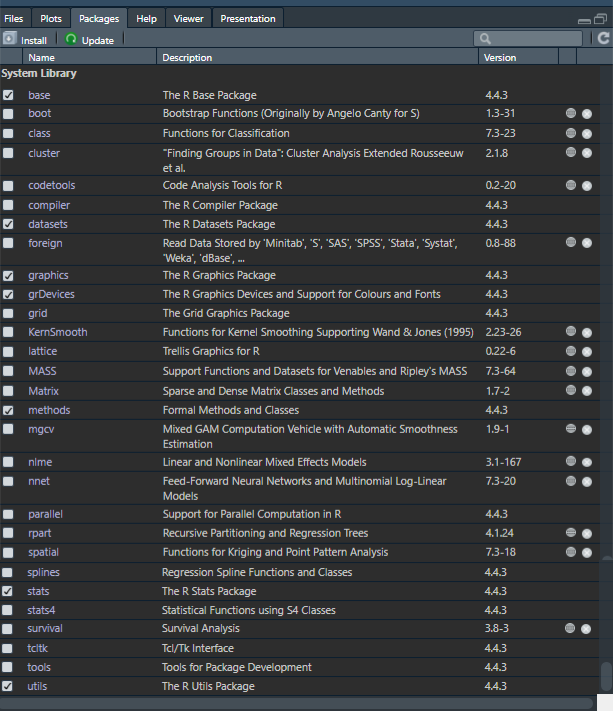
\includegraphics[width=0.75\linewidth,height=\textheight,keepaspectratio]{unidad_1/images/rbase_paquetes.png}
\end{center}

En la actualidad, existen más de 17.000 paquetes disponibles para una
amplia variedad de aplicaciones, número que crece mes a mes gracias a la
naturaleza \emph{open source} del lenguaje. Cualquier persona puede
desarrollar y compartir sus propios paquetes, aunque no todos llegan a
publicarse en el repositorio oficial CRAN (Comprehensive R Archive
Network), que actúa como principal fuente de distribución.

Los paquetes pueden descargarse directamente desde CRAN o instalarse a
partir de archivos comprimidos locales (como \texttt{.zip} o
\texttt{.tar.gz}). Una vez instalados, se los puede activar en cualquier
análisis.

\subsection{Dependencias}\label{dependencias}

En muchos casos, al utilizar un paquete, este necesita de otros para
funcionar correctamente. Esta relación se conoce como
\textbf{dependencia}, y es una característica central en el ecosistema
de R.

La mayoría de las funciones incluidas en los paquetes están
desarrolladas en el propio lenguaje R y, durante su construcción, es
habitual que recurran a funciones ya existentes en otros paquetes. Por
ejemplo, una función nueva puede hacer uso de una función auxiliar que
no pertenece al sistema base, sino a otro paquete externo.

Cuando intentamos ejecutar una función que depende de otras no
disponibles en nuestra instalación, R no podrá encontrar esas funciones
y nos devolverá un mensaje de error indicando que no reconoce el nombre
solicitado. Este tipo de errores suele alertar sobre funciones
``desconocidas'' o ``no encontradas'', lo que indica que falta instalar
o activar alguno de los paquetes requeridos.

Para evitar estos inconvenientes, R intenta resolver automáticamente las
dependencias cuando instalamos un paquete desde el repositorio oficial
CRAN. Si el paquete necesita otros para funcionar, el sistema detecta
esta relación y se encarga de instalar también aquellos paquetes
auxiliares. De todos modos, si alguno no se instala correctamente o no
se activa en la sesión, será necesario hacerlo de forma manual.

\section{Errores y advertencias}\label{errores-y-advertencias}

El lenguaje R es muy preciso en su sintaxis. Cometer errores al escribir
funciones u objetos es común durante el aprendizaje, y el intérprete de
R devuelve mensajes de error cuando detecta algo incorrecto.

Uno de los aspectos clave a tener en cuenta es que R \textbf{distingue
entre mayúsculas y minúsculas} (\emph{case sensitive}), por lo que no es
lo mismo escribir \texttt{a} que \texttt{A}.

Existen tres grupos de mensajes de error:

\begin{itemize}
\item
  Errores de sintaxis
\item
  Error de objeto no encontrado
\item
  Otros errores
\end{itemize}

\subsection{Errores de sintaxis}\label{errores-de-sintaxis}

Ocurre cuando R no puede interpretar una línea de código porque algo
está mal escrito. Los errores de sintaxis más frecuentes incluyen:

\begin{itemize}
\item
  Paréntesis, comas, comillas, corchetes o llaves mal colocados o
  ausentes.
\item
  Argumentos mal separados o incorrectamente definidos.
\end{itemize}

Por ejemplo la función \texttt{rep()} repite valores una cantidad de
veces. Tiene dos argumentos, \texttt{x} donde se coloca el valor a
repetir y \texttt{times} donde se define la cantidad de veces:

\begin{Shaded}
\begin{Highlighting}[]
\FunctionTok{rep}\NormalTok{(}\AttributeTok{x =} \DecValTok{3}\NormalTok{, }\AttributeTok{times =} \DecValTok{4}\NormalTok{) }\CommentTok{\# repetimos 4 veces 3 con rep()}
\end{Highlighting}
\end{Shaded}

\begin{verbatim}
[1] 3 3 3 3
\end{verbatim}

Si nos olvidamos de cerrar el paréntesis:

\begin{Shaded}
\begin{Highlighting}[]
\FunctionTok{rep}\NormalTok{(}\AttributeTok{x =} \DecValTok{3}\NormalTok{, }\AttributeTok{times =} \DecValTok{4}
\end{Highlighting}
\end{Shaded}

\begin{verbatim}
Error in parse(text = input): <text>:2:0: unexpected end of input
1: rep(x = 3, times = 4
   ^
\end{verbatim}

Si omitimos la coma entre argumentos:

\begin{Shaded}
\begin{Highlighting}[]
\FunctionTok{rep}\NormalTok{(}\AttributeTok{x =} \DecValTok{3} \AttributeTok{times =} \DecValTok{4}\NormalTok{)}
\end{Highlighting}
\end{Shaded}

\begin{verbatim}
Error in parse(text = input): <text>:1:11: unexpected symbol
1: rep(x = 3 times
              ^
\end{verbatim}

Si usamos un nombre de argumento no válido:

\begin{Shaded}
\begin{Highlighting}[]
\FunctionTok{rep}\NormalTok{(}\AttributeTok{y =} \DecValTok{3}\NormalTok{, }\AttributeTok{times =} \DecValTok{4}\NormalTok{)}
\end{Highlighting}
\end{Shaded}

\begin{verbatim}
Error in `rep()`:
! attempt to replicate an object of type 'symbol'
\end{verbatim}

Si escribimos mal el nombre de la función:

\begin{Shaded}
\begin{Highlighting}[]
\FunctionTok{rop}\NormalTok{(}\AttributeTok{x =} \DecValTok{3}\NormalTok{, }\AttributeTok{times =} \DecValTok{4}\NormalTok{)}
\end{Highlighting}
\end{Shaded}

\begin{verbatim}
Error in `rop()`:
! could not find function "rop"
\end{verbatim}

Este último error se asemeja a un error de objeto no encontrado, aunque
tiene origen en un problema de sintaxis.

Los mensajes de error en general y sobre todo al principio pueden
parecer extraños y difíciles de entender, pero con un poco de práctica
podemos inferir donde está el problema.

\subsection{Error de objeto no
encontrado}\label{error-de-objeto-no-encontrado}

Este tipo de error se produce cuando R no reconoce un objeto utilizado
en el código. Las causas más frecuentes incluyen:

\begin{itemize}
\item
  El nombre del objeto está mal escrito (por ejemplo, errores de
  sintaxis o uso incorrecto de mayúsculas/minúsculas).
\item
  El objeto pertenece a un paquete o archivo que no fue cargado.
\item
  Faltan comillas al declarar caracteres.
\item
  Otras causas similares.
\end{itemize}

Volvamos al ejemplo anterior, ahora repitiendo un valor tipo
\texttt{character}:

\begin{Shaded}
\begin{Highlighting}[]
\FunctionTok{rep}\NormalTok{(}\AttributeTok{x =} \StringTok{"A"}\NormalTok{, }\AttributeTok{times =} \DecValTok{4}\NormalTok{) }\CommentTok{\# repetimos 4 veces "A" con rep()}
\end{Highlighting}
\end{Shaded}

\begin{verbatim}
[1] "A" "A" "A" "A"
\end{verbatim}

Si olvidamos las comillas:

\begin{Shaded}
\begin{Highlighting}[]
\FunctionTok{rep}\NormalTok{(}\AttributeTok{x =}\NormalTok{ A, }\AttributeTok{times =} \DecValTok{4}\NormalTok{) }\CommentTok{\# repetimos 4 veces A con rep()}
\end{Highlighting}
\end{Shaded}

\begin{verbatim}
Error:
! object 'A' not found
\end{verbatim}

\subsection{Otros errores}\label{otros-errores}

Son aquellos que se generan por causas distintas a errores de sintaxis o
de objeto no encontrado. Por ejemplo:

\begin{Shaded}
\begin{Highlighting}[]
\StringTok{"x"} \SpecialCharTok{+} \DecValTok{10}
\end{Highlighting}
\end{Shaded}

\begin{verbatim}
Error in `"x" + 10`:
! non-numeric argument to binary operator
\end{verbatim}

El código anterior genera un mensaje de error porque intenta sumar
objetos de tipos incompatibles entre sí.

Veamos otro ejemplo:

\begin{Shaded}
\begin{Highlighting}[]
\FunctionTok{t.test}\NormalTok{(}\DecValTok{1}\NormalTok{)}
\end{Highlighting}
\end{Shaded}

\begin{verbatim}
Error in `t.test.default()`:
! not enough 'x' observations
\end{verbatim}

En este caso, el error se debe a que no hay suficientes observaciones
para realizar una prueba \(t\) de Student.

Otro caso frecuente ocurre cuando se intenta acceder a una posición
inexistente en un vector:

\begin{Shaded}
\begin{Highlighting}[]
\NormalTok{x }\OtherTok{\textless{}{-}} \FunctionTok{c}\NormalTok{(}\DecValTok{1}\NormalTok{, }\DecValTok{2}\NormalTok{, }\DecValTok{3}\NormalTok{)}
\NormalTok{x[[}\DecValTok{5}\NormalTok{]]}
\end{Highlighting}
\end{Shaded}

\begin{verbatim}
Error in `x[[5]]`:
! subscript out of bounds
\end{verbatim}

Este mensaje de error indica que el subíndice está fuera de los límites
del objeto (\texttt{subscript\ out\ of\ bounds}).

\subsection{Advertencias}\label{advertencias}

Las advertencia no son tan serias como un error, o al menos no lo
parece, ya que permiten el código se ejecute igual. Pero puede ocurrir
que ignorar una advertencia llegue a ser algo muy serio, si esto implica
que la salida de la función es equivocada.

Ignorar advertencias puede llevar a conclusiones erróneas, por lo que es
recomendable prestarles atención y entender su causa.

Por ejemplo:

\begin{Shaded}
\begin{Highlighting}[]
\FunctionTok{log}\NormalTok{(}\SpecialCharTok{{-}}\DecValTok{1}\NormalTok{)}
\end{Highlighting}
\end{Shaded}

\begin{verbatim}
Warning in log(-1): NaNs produced
\end{verbatim}

\begin{verbatim}
[1] NaN
\end{verbatim}

la función genera una advertencia porque el logaritmo de un número
negativo no está definido en los reales, y R devuelve un valor
\texttt{NaN} (\emph{Not a Number}).

\subsection{Resumiendo\ldots{}}\label{resumiendo}

\protect\phantomsection\label{fig1}
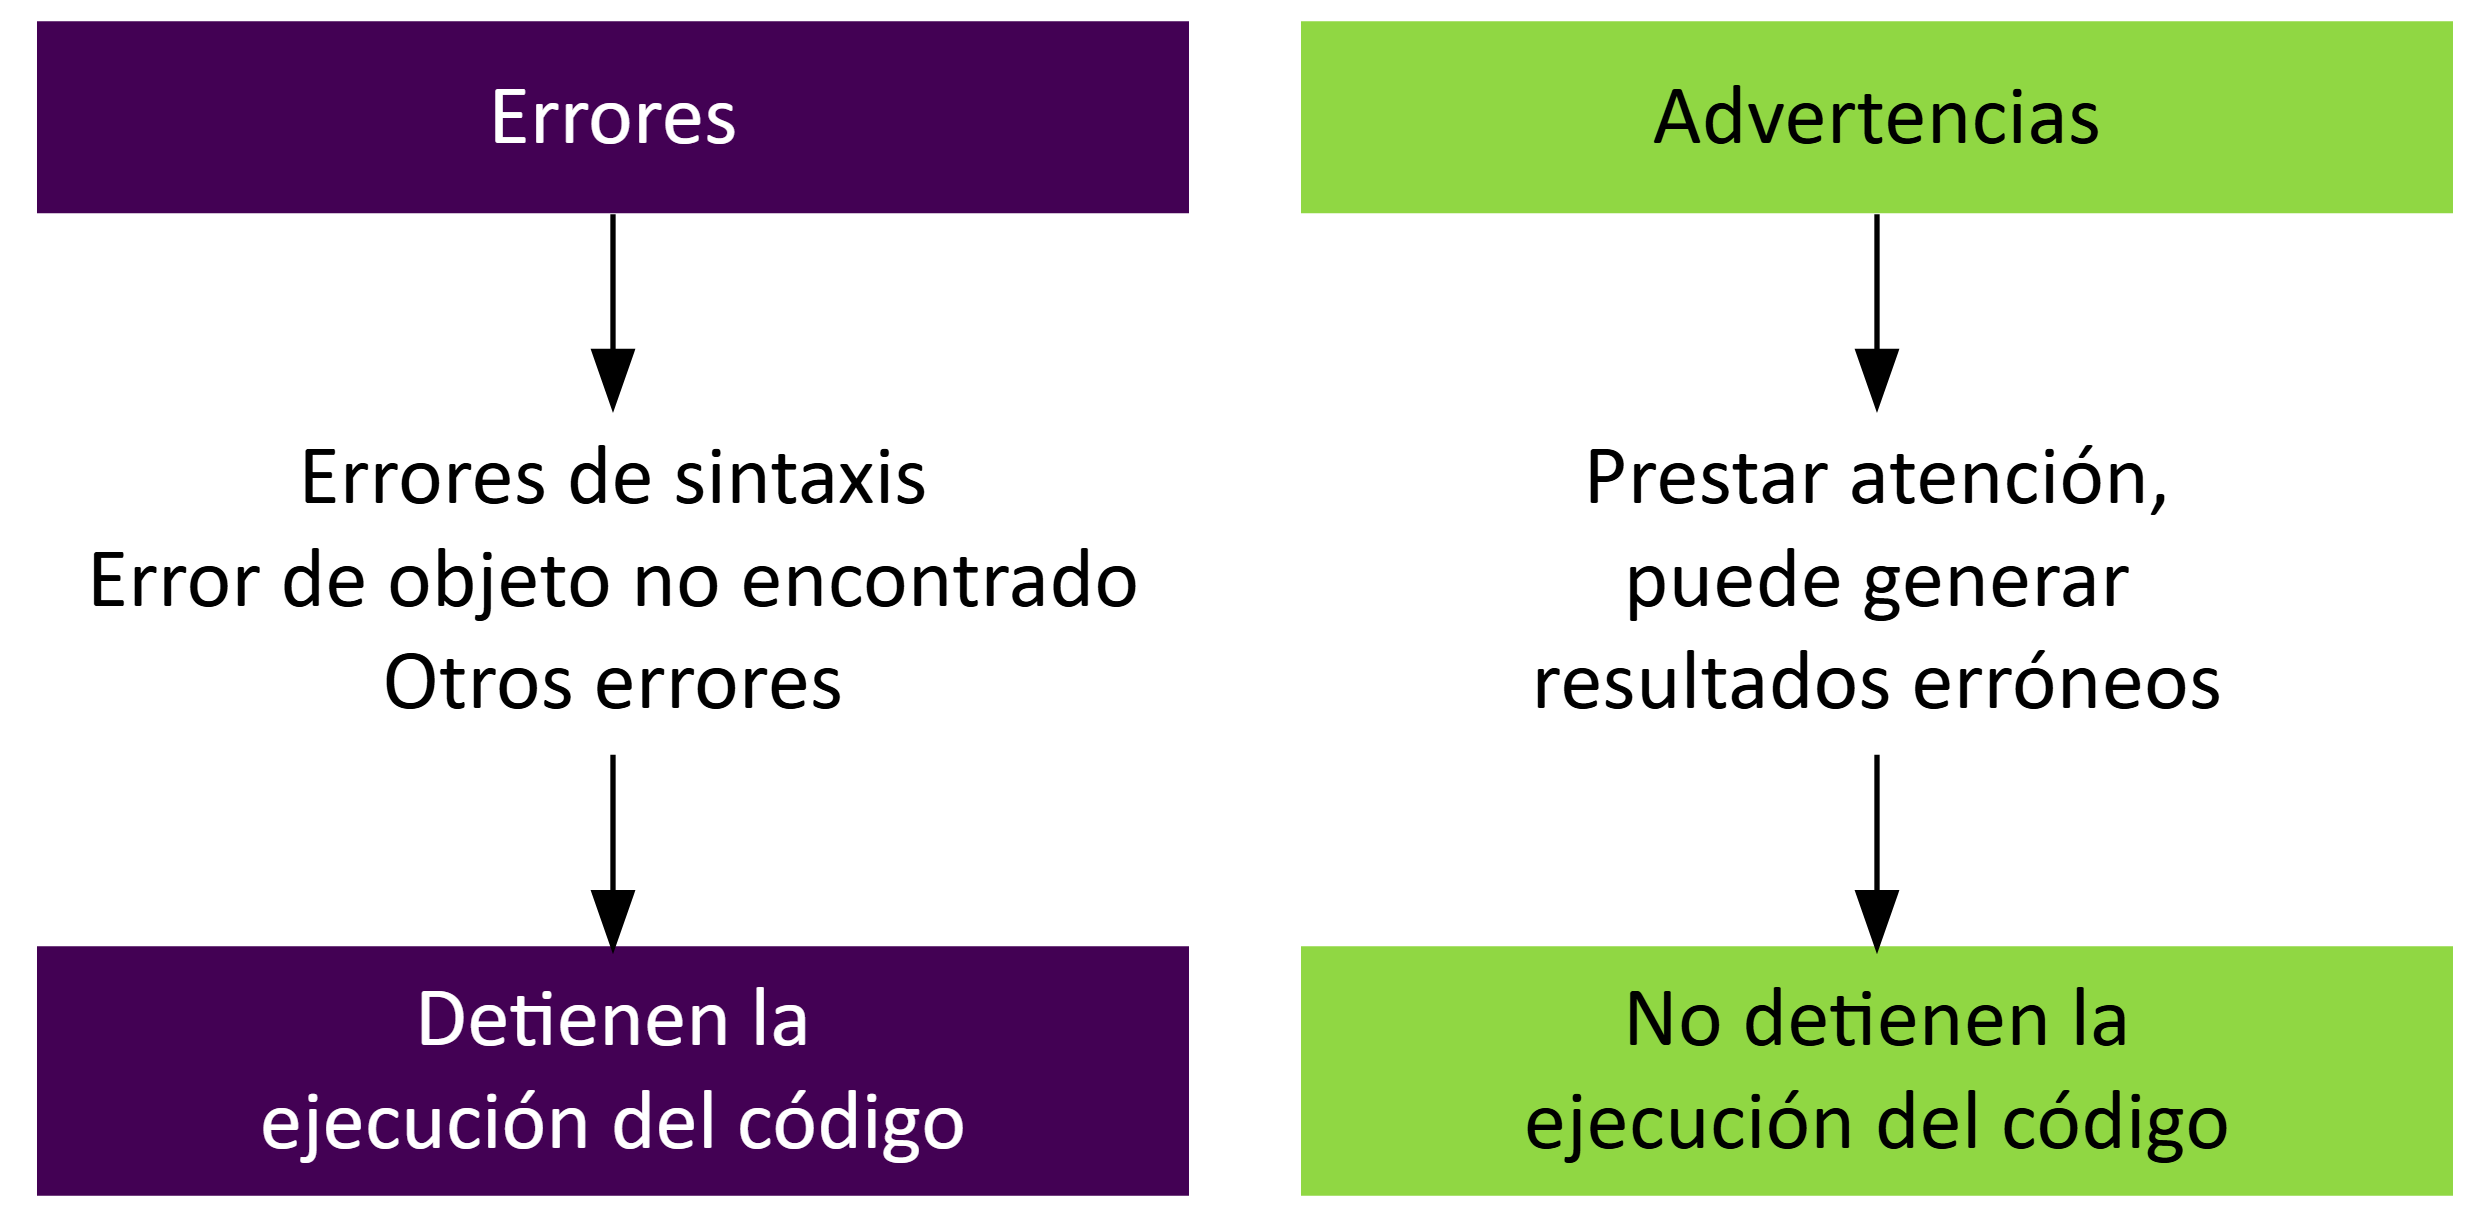
\includegraphics[width=5.5in,height=3.5in]{unidad_1/01_intro_R_files/figure-latex/dot-figure-3.png}

\section{Creación de objetos}\label{creaciuxf3n-de-objetos}

Todas las declaraciones donde se crean objetos usan el símbolo de
asignación \texttt{\textless{}-}:

\begin{Shaded}
\begin{Highlighting}[]
\NormalTok{nombre\_objeto }\OtherTok{\textless{}{-}}\NormalTok{ valor}
\end{Highlighting}
\end{Shaded}

Veámoslo en un ejemplo:

\begin{Shaded}
\begin{Highlighting}[]
\NormalTok{a }\OtherTok{\textless{}{-}} \DecValTok{1}
\end{Highlighting}
\end{Shaded}

En este caso asignamos el valor 1 al objeto \texttt{a}. El objeto
\texttt{a} es un vector de una posición (un solo valor). Si llamamos al
objeto, el intérprete devuelve el valor asignado previamente:

\begin{Shaded}
\begin{Highlighting}[]
\NormalTok{a}
\end{Highlighting}
\end{Shaded}

\begin{verbatim}
[1] 1
\end{verbatim}

Observemos que, además de devolvernos el valor, aparece delante un
número entre corchetes \texttt{{[}1{]}}. Este número es la ubicación o
\textbf{índice} del comienzo del objeto. En este caso, como el vector
tiene una sola posición, indica que el primer valor mostrado empieza en
la posición 1.

\section{Estructuras de datos}\label{estructuras-de-datos}

Los objetos contenedores de datos más simples pertenecen a cinco clases
atómicas, que son:

\begin{itemize}
\item
  \texttt{integer} (números enteros)
\item
  \texttt{numeric} (números reales)
\item
  \texttt{complex} (números complejos)
\item
  \texttt{character} (cadenas de caracteres)
\item
  \texttt{logical} (valores lógicos: \texttt{TRUE} o \texttt{FALSE})
\end{itemize}

\protect\phantomsection\label{fig2}
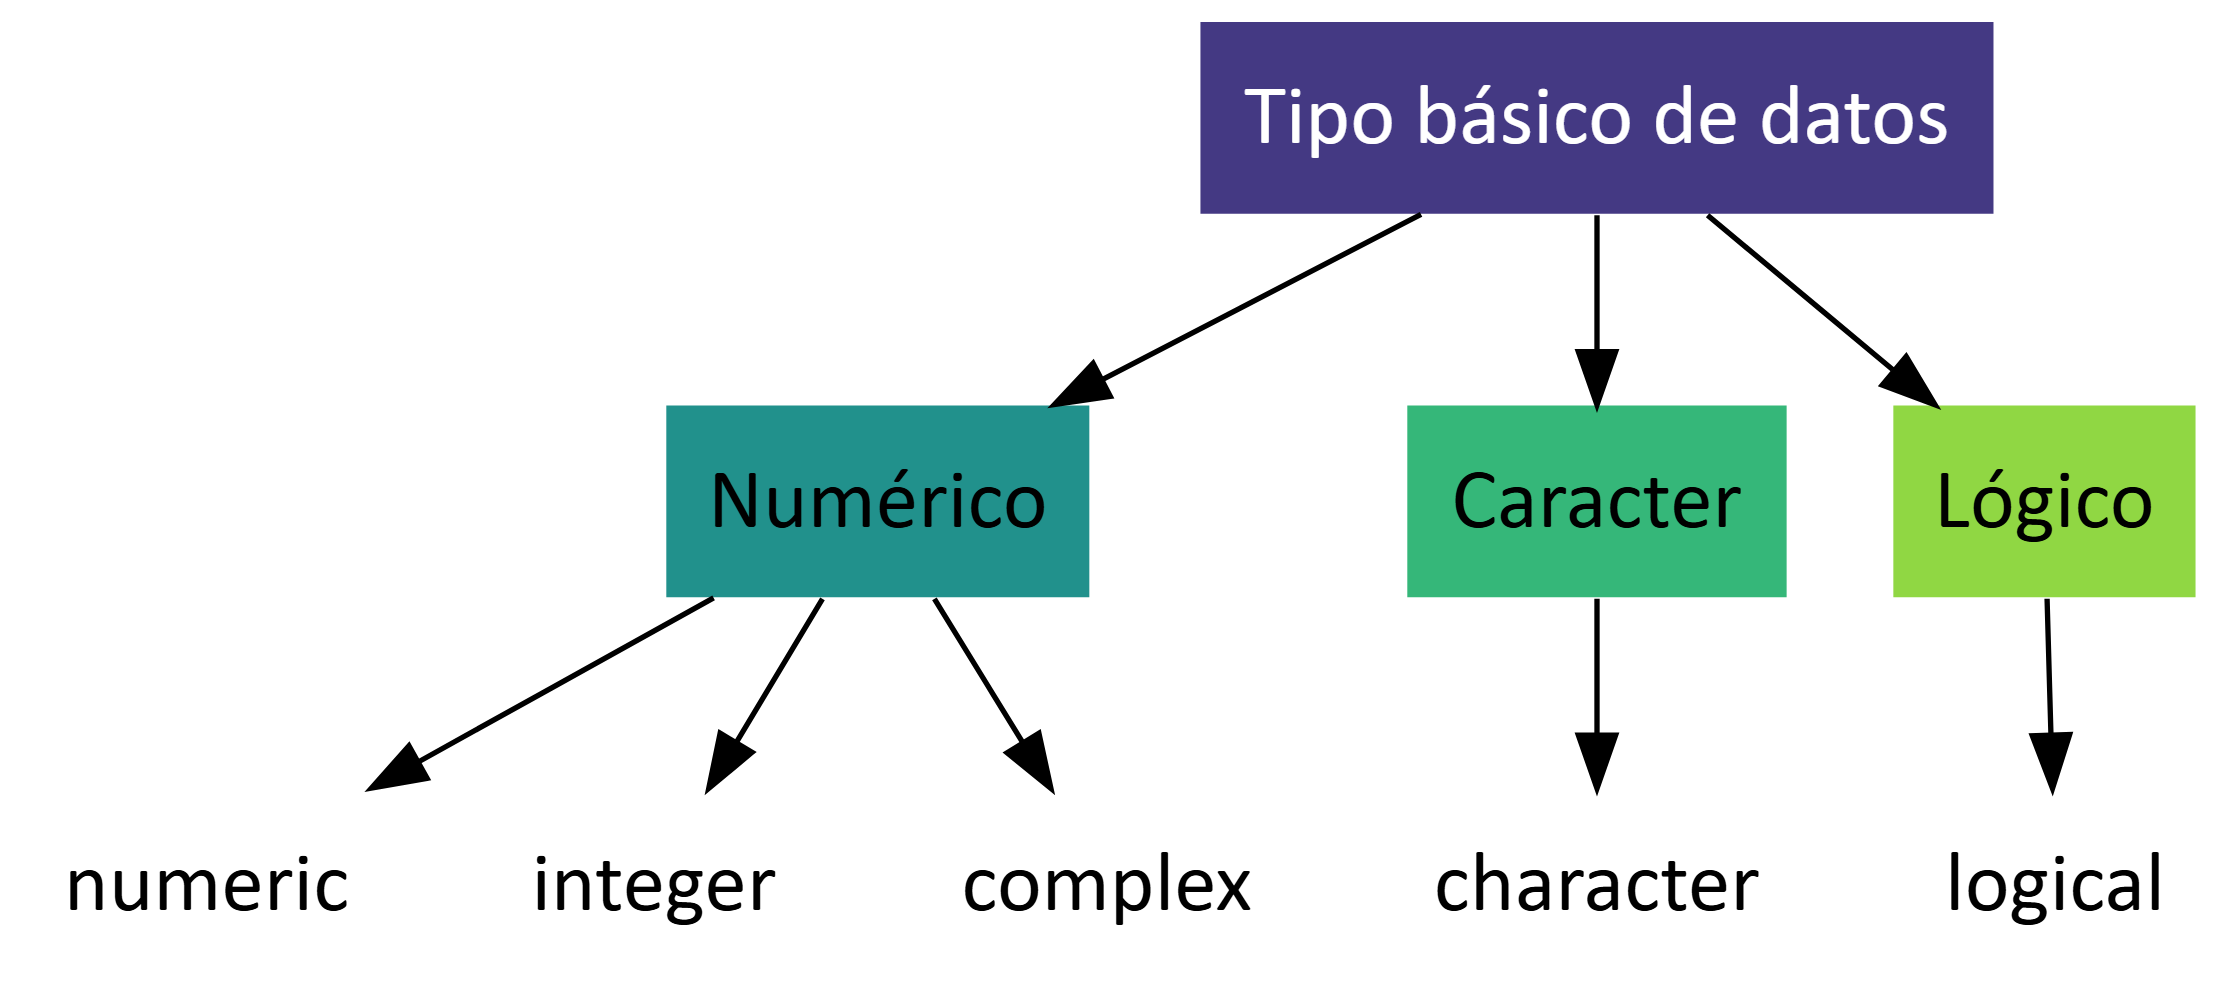
\includegraphics[width=5.5in,height=3.5in]{unidad_1/01_intro_R_files/figure-latex/dot-figure-4.png}

Sin embargo, cada una de estas clases de datos no se encuentran de
manera aislada, sino encapsuladas dentro de la clase de objeto más
básica de R, a la que se denomina \textbf{vector}.

En RStudio, el sistema de colores ayuda a distinguir los tipos de
valores:

\begin{Shaded}
\begin{Highlighting}[]
\CommentTok{\# Número}
\DecValTok{1111}
\end{Highlighting}
\end{Shaded}

\begin{verbatim}
[1] 1111
\end{verbatim}

\begin{Shaded}
\begin{Highlighting}[]
\CommentTok{\# Caracter}
\StringTok{"esto es una cadena de texto"}
\end{Highlighting}
\end{Shaded}

\begin{verbatim}
[1] "esto es una cadena de texto"
\end{verbatim}

\begin{Shaded}
\begin{Highlighting}[]
\CommentTok{\# Lógico}
\ConstantTok{TRUE}
\end{Highlighting}
\end{Shaded}

\begin{verbatim}
[1] TRUE
\end{verbatim}

\begin{Shaded}
\begin{Highlighting}[]
\CommentTok{\# Objeto}
\NormalTok{a }\OtherTok{\textless{}{-}} \DecValTok{1}
\end{Highlighting}
\end{Shaded}

\subsection{Vectores}\label{vectores}

Un vector es un conjunto de valores (números o símbolos), del mismo tipo
ordenados de la forma (elemento 1, elemento 2, \ldots{} , elemento
\(n\)), donde \(n\) es la longitud o tamaño del vector.

Los atributos principales son:

\begin{itemize}
\item
  \textbf{Tipo}: puede ser \texttt{integer}, \texttt{numeric},
  \texttt{character}, \texttt{complex} o \texttt{logical}.
\item
  \textbf{Longitud}: cantidad de elementos que contiene el objeto,
\end{itemize}

El vector más simple contiene un solo dato, por ejemplo un vector de
longitud 1 y tipo \texttt{numeric}:

\begin{Shaded}
\begin{Highlighting}[]
\NormalTok{vec1 }\OtherTok{\textless{}{-}} \DecValTok{1}
\NormalTok{vec1}
\end{Highlighting}
\end{Shaded}

\begin{verbatim}
[1] 1
\end{verbatim}

Otro vector más grande por ejemplo podría ser \texttt{(1,\ 5,\ 2)}. En
este caso también es del tipo \texttt{numeric} pero tiene una longitud
de 3 elementos:

\begin{Shaded}
\begin{Highlighting}[]
\NormalTok{vec2 }\OtherTok{\textless{}{-}} \FunctionTok{c}\NormalTok{(}\DecValTok{1}\NormalTok{, }\DecValTok{5}\NormalTok{, }\DecValTok{2}\NormalTok{)}
\NormalTok{vec2}
\end{Highlighting}
\end{Shaded}

\begin{verbatim}
[1] 1 5 2
\end{verbatim}

Para concatenar elementos usamos la función \texttt{c()}, dentro de la
cual van los valores separados por comas. El orden de los elementos
importa, en nuestro ejemplo la primera posición la ocupa el 1, la
segunda el 5 y la tercera el 2. Si tuvieramos otro vector
\texttt{(5,\ 1,\ 2)}, no sería lo mismo porque los valores están
ordenados de forma diferente.

Para conocer la longitud del vector usamos:

\begin{Shaded}
\begin{Highlighting}[]
\FunctionTok{length}\NormalTok{(vec2)}
\end{Highlighting}
\end{Shaded}

\begin{verbatim}
[1] 3
\end{verbatim}

Nos informa que \texttt{vec2} tiene 3 elementos.

Para conocer el tipo de dato ejecutamos:

\begin{Shaded}
\begin{Highlighting}[]
\FunctionTok{class}\NormalTok{(vec2)}
\end{Highlighting}
\end{Shaded}

\begin{verbatim}
[1] "numeric"
\end{verbatim}

Podemos ver que los datos almacenados en este segundo ejemplo cumplen
con la definición en lo que respecta al tipo de dato, ya que cada
elemento es del mismo tipo (\texttt{numeric}).

Veamos un ejemplo de asignación de otro tipo de dato atómico, como es el
\texttt{character}:

\begin{Shaded}
\begin{Highlighting}[]
\NormalTok{vec3 }\OtherTok{\textless{}{-}} \StringTok{"Hola"}
\NormalTok{vec3}
\end{Highlighting}
\end{Shaded}

\begin{verbatim}
[1] "Hola"
\end{verbatim}

Siempre que escribamos contenido de tipo \texttt{character} debemos
hacerlo entre comillas. En este caso generamos el vector \texttt{vec3}
con el contenido \texttt{"Hola"}, que, a pesar de ser una palabra
compuesta de varios caracteres, dentro del vector \texttt{vec3} esta
ocupa una sola posición:

\begin{Shaded}
\begin{Highlighting}[]
\FunctionTok{length}\NormalTok{(vec3)}
\end{Highlighting}
\end{Shaded}

\begin{verbatim}
[1] 1
\end{verbatim}

Respecto al tipo de dato si usamos la función \texttt{class()}
tendremos:

\begin{Shaded}
\begin{Highlighting}[]
\FunctionTok{class}\NormalTok{(vec3)}
\end{Highlighting}
\end{Shaded}

\begin{verbatim}
[1] "character"
\end{verbatim}

\subsection{Factores}\label{factores}

Un factor es un objeto especialmente diseñado para contener datos
categóricos y se asocia particularmente con las \emph{variables
cualitativas}.

En su estructura interna está compuesto por dos vectores:

\begin{itemize}
\item
  Un vector de índices enteros.
\item
  Un vector de categorías (niveles) de tipo \texttt{character}, a los
  que hace referencia el primer vector.
\end{itemize}

Existen de dos tipos: factores nominales y factores ordinales. En el
caso del segundo se establece un orden en los niveles.

Normalmente, obtenemos un tipo \texttt{factor} de convertir un vector u
otro tipo de objeto con caracteres, pero para mostrar un ejemplo lo
realizamos con la función \texttt{factor()}:

\begin{Shaded}
\begin{Highlighting}[]
\NormalTok{factor1 }\OtherTok{\textless{}{-}} \FunctionTok{factor}\NormalTok{(}
  \AttributeTok{x =} \FunctionTok{c}\NormalTok{(}\StringTok{"a"}\NormalTok{, }\StringTok{"b"}\NormalTok{, }\StringTok{"a"}\NormalTok{, }\StringTok{"c"}\NormalTok{, }\StringTok{"b"}\NormalTok{, }\StringTok{"a"}\NormalTok{),}
  \AttributeTok{levels =} \FunctionTok{c}\NormalTok{(}\StringTok{"a"}\NormalTok{, }\StringTok{"b"}\NormalTok{, }\StringTok{"c"}\NormalTok{)}
\NormalTok{)}
\NormalTok{factor1}
\end{Highlighting}
\end{Shaded}

\begin{verbatim}
[1] a b a c b a
Levels: a b c
\end{verbatim}

Creamos el objeto \texttt{factor}1 con 6 elementos caracteres y tres
niveles sin orden.

Además de la practicidad de trabajar con factores, muchas funciones de R
requieren que las variables categóricas estén en formato factor para
funcionar correctamente.

\subsection{\texorpdfstring{\emph{Dataframe}}{Dataframe}}\label{dataframe}

Un \emph{dataframe} es un objeto diseñado para contener conjuntos de
datos y representa una estructura bidimensional similar a una tabla, con
filas y columnas. Cada columna puede almacenar elementos de distintos
tipos (por ejemplo, numéricos, de texto o lógicos), siempre que todos
tengan la misma longitud.

Las columnas suelen tener nombres únicos, lo que permite referenciarlas
fácilmente como si fueran variables individuales dentro del conjunto de
datos.

Este es el tipo de objeto que se utiliza habitualmente para almacenar
información importada desde archivos externos (por ejemplo, archivos de
texto separados por comas o planillas de Excel), y con el que más
frecuentemente trabajamos en los análisis.

Desde el punto de vista estructural, un \emph{dataframe} está compuesto
por una serie de vectores de igual longitud dispuestos verticalmente,
uno al lado del otro, conformando las columnas de la tabla.

Veamos un ejemplo:

\begin{Shaded}
\begin{Highlighting}[]
\CommentTok{\# Historia clínica}
\NormalTok{HC }\OtherTok{\textless{}{-}} \FunctionTok{c}\NormalTok{(}\StringTok{"F324"}\NormalTok{, }\StringTok{"G21"}\NormalTok{, }\StringTok{"G34"}\NormalTok{, }\StringTok{"F231"}\NormalTok{)}

\CommentTok{\# Edad}
\NormalTok{edad }\OtherTok{\textless{}{-}} \FunctionTok{c}\NormalTok{(}\DecValTok{34}\NormalTok{, }\DecValTok{32}\NormalTok{, }\DecValTok{34}\NormalTok{, }\DecValTok{54}\NormalTok{)}

\CommentTok{\# Sexo}
\NormalTok{sexo }\OtherTok{\textless{}{-}} \FunctionTok{c}\NormalTok{(}\StringTok{"M"}\NormalTok{, }\StringTok{"V"}\NormalTok{, }\StringTok{"V"}\NormalTok{, }\StringTok{"M"}\NormalTok{)}

\CommentTok{\# dataframe}
\NormalTok{df1 }\OtherTok{\textless{}{-}} \FunctionTok{data.frame}\NormalTok{(HC, edad, sexo)}

\NormalTok{df1}
\end{Highlighting}
\end{Shaded}

\begin{verbatim}
    HC edad sexo
1 F324   34    M
2  G21   32    V
3  G34   34    V
4 F231   54    M
\end{verbatim}

Creamos tres vectores con datos de supuestos individuos, su historia
clinica, la edad y el sexo. Luego mediante la función
\texttt{data.frame()} ``unimos'' esos vectores en forma vertical para
formar un \emph{dataframe} de 3 variables y 4 observaciones.

\begin{tcolorbox}[enhanced jigsaw, arc=.35mm, bottomrule=.15mm, breakable, colback=white, colframe=quarto-callout-warning-color-frame, left=2mm, leftrule=.75mm, opacityback=0, rightrule=.15mm, toprule=.15mm]
\begin{minipage}[t]{5.5mm}
\textcolor{quarto-callout-warning-color}{\faExclamationTriangle}
\end{minipage}%
\begin{minipage}[t]{\textwidth - 5.5mm}

Existen otras estructuras de datos que aparecen en la siguiente figura.
Las más habituales en nuestro trabajo son los vectores y los
\emph{dataframes}. Los factores serán necesarios cuando tengamos que
especificar distintos órdenes de niveles.

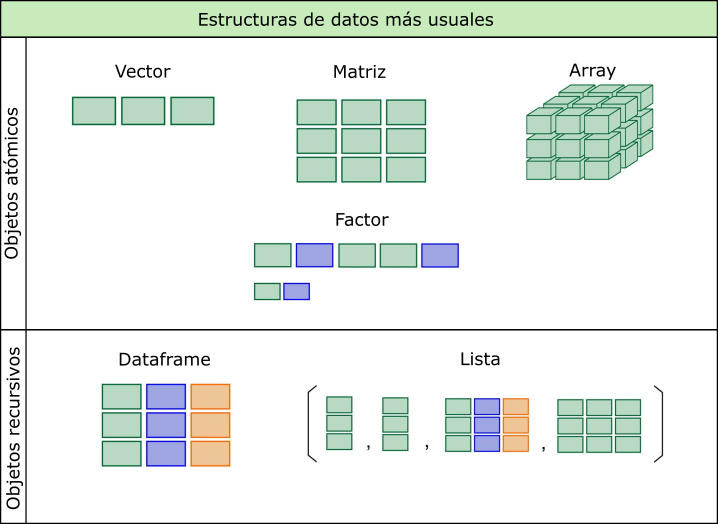
\includegraphics[width=6.25in,height=\textheight,keepaspectratio]{unidad_1/images/objetos_R.png}

\end{minipage}%
\end{tcolorbox}

\section{Operadores}\label{operadores}

Además de funciones, el lenguaje R cuenta con operadores de uso
relativamente intuitivo, que permiten realizar operaciones de diferentes
tipos con los objetos que contienen datos.

\subsection{Operadores aritméticos}\label{operadores-aritmuxe9ticos}

{\def\LTcaptype{none} % do not increment counter
\begin{longtable}[]{@{}ll@{}}
\toprule\noalign{}
Operador & Descripción \\
\midrule\noalign{}
\endhead
\bottomrule\noalign{}
\endlastfoot
+ & Suma \\
- & Resta \\
* & Multiplicación \\
/ & División \\
\^{} & Potencia \\
\%\% & Módulo \\
\%/\% & División de enteros \\
\end{longtable}
}

Los operadores aritméticos se utilizan como si el lenguaje fuese una
calculadora:

\begin{Shaded}
\begin{Highlighting}[]
\CommentTok{\# Suma}
\DecValTok{2} \SpecialCharTok{+} \DecValTok{5}
\end{Highlighting}
\end{Shaded}

\begin{verbatim}
[1] 7
\end{verbatim}

\begin{Shaded}
\begin{Highlighting}[]
\CommentTok{\# Resta}
\DecValTok{3} \SpecialCharTok{{-}} \DecValTok{2}
\end{Highlighting}
\end{Shaded}

\begin{verbatim}
[1] 1
\end{verbatim}

\begin{Shaded}
\begin{Highlighting}[]
\CommentTok{\# Multiplicación}
\DecValTok{9} \SpecialCharTok{*} \DecValTok{3}
\end{Highlighting}
\end{Shaded}

\begin{verbatim}
[1] 27
\end{verbatim}

\begin{Shaded}
\begin{Highlighting}[]
\CommentTok{\# División}
\DecValTok{10} \SpecialCharTok{/} \DecValTok{2}
\end{Highlighting}
\end{Shaded}

\begin{verbatim}
[1] 5
\end{verbatim}

\begin{Shaded}
\begin{Highlighting}[]
\CommentTok{\# Potencia}
\DecValTok{5}\SpecialCharTok{\^{}}\DecValTok{2}
\end{Highlighting}
\end{Shaded}

\begin{verbatim}
[1] 25
\end{verbatim}

También se pueden hacer operaciones con los objetos que almacenan
valores numéricos:

\begin{Shaded}
\begin{Highlighting}[]
\NormalTok{a }\OtherTok{\textless{}{-}} \DecValTok{3}

\NormalTok{b }\OtherTok{\textless{}{-}} \DecValTok{6}

\NormalTok{(a }\SpecialCharTok{+}\NormalTok{ b) }\SpecialCharTok{*}\NormalTok{ b}
\end{Highlighting}
\end{Shaded}

\begin{verbatim}
[1] 54
\end{verbatim}

Y funciona con objetos con más de un elemento, aplicando aritmética
vectorial, donde las operaciones se realizan elemento a elemento:

\begin{Shaded}
\begin{Highlighting}[]
\NormalTok{a }\OtherTok{\textless{}{-}} \FunctionTok{c}\NormalTok{(}\DecValTok{1}\NormalTok{, }\DecValTok{2}\NormalTok{, }\DecValTok{3}\NormalTok{)}

\NormalTok{a }\SpecialCharTok{*} \DecValTok{3}
\end{Highlighting}
\end{Shaded}

\begin{verbatim}
[1] 3 6 9
\end{verbatim}

O bien, con operaciones entre los objetos, donde se realiza entre los
elementos de la misma posición:

\begin{Shaded}
\begin{Highlighting}[]
\NormalTok{a }\OtherTok{\textless{}{-}} \FunctionTok{c}\NormalTok{(}\DecValTok{1}\NormalTok{, }\DecValTok{2}\NormalTok{, }\DecValTok{3}\NormalTok{)}

\NormalTok{a }\SpecialCharTok{*}\NormalTok{ a}
\end{Highlighting}
\end{Shaded}

\begin{verbatim}
[1] 1 4 9
\end{verbatim}

\subsection{Operadores relacionales}\label{operadores-relacionales}

{\def\LTcaptype{none} % do not increment counter
\begin{longtable}[]{@{}ll@{}}
\toprule\noalign{}
Operador & Descripción \\
\midrule\noalign{}
\endhead
\bottomrule\noalign{}
\endlastfoot
\textless{} & Menor que \\
\textgreater{} & Mayor que \\
\textless= & Menor o igual que \\
\textgreater= & Mayor o igual que \\
== & Igual que \\
!= & No igual que \\
\end{longtable}
}

Habitualmente estos operadores se utilizan asiduamente en expresiones
para indicar relaciones entre valores.

Podemos ver su funcionamiento en el ejemplo siguiente:

\begin{Shaded}
\begin{Highlighting}[]
\NormalTok{a }\OtherTok{\textless{}{-}} \FunctionTok{c}\NormalTok{(}\DecValTok{3}\NormalTok{, }\DecValTok{8}\NormalTok{, }\DecValTok{2}\NormalTok{)}

\NormalTok{a }\SpecialCharTok{==} \FunctionTok{c}\NormalTok{(}\DecValTok{3}\NormalTok{, }\DecValTok{4}\NormalTok{, }\DecValTok{5}\NormalTok{)}
\end{Highlighting}
\end{Shaded}

\begin{verbatim}
[1]  TRUE FALSE FALSE
\end{verbatim}

El lenguaje evalúa las comparaciones que hace el operador relacional
igual (en este caso) y en aquellos valores que coinciden devuelve
\texttt{TRUE} y en los que no hay coincidencia devuelve \texttt{FALSE}.

Lo mismo sucede con los otros operadores relacionales:

\begin{Shaded}
\begin{Highlighting}[]
\NormalTok{a }\OtherTok{\textless{}{-}} \FunctionTok{c}\NormalTok{(}\DecValTok{4}\NormalTok{, }\DecValTok{8}\NormalTok{, }\DecValTok{10}\NormalTok{)}

\NormalTok{a }\SpecialCharTok{\textgreater{}} \DecValTok{8}
\end{Highlighting}
\end{Shaded}

\begin{verbatim}
[1] FALSE FALSE  TRUE
\end{verbatim}

\begin{Shaded}
\begin{Highlighting}[]
\NormalTok{a }\SpecialCharTok{\textless{}} \DecValTok{8}
\end{Highlighting}
\end{Shaded}

\begin{verbatim}
[1]  TRUE FALSE FALSE
\end{verbatim}

\begin{Shaded}
\begin{Highlighting}[]
\NormalTok{a }\SpecialCharTok{!=} \DecValTok{8}
\end{Highlighting}
\end{Shaded}

\begin{verbatim}
[1]  TRUE FALSE  TRUE
\end{verbatim}

\subsection{Operadores lógicos}\label{operadores-luxf3gicos}

{\def\LTcaptype{none} % do not increment counter
\begin{longtable}[]{@{}ll@{}}
\toprule\noalign{}
Operador & Descripción \\
\midrule\noalign{}
\endhead
\bottomrule\noalign{}
\endlastfoot
! & NOT \\
\& & AND booleano \\
\&\& & AND booleano para vectores de longitud 1 \\
\textbar{} & OR booleano \\
\textbar\textbar{} & OR booleano para vectores de longitud 1 \\
\end{longtable}
}

Cuando queremos conectar algunas de las expresiones relacionales hacemos
uso de estos operadores lógicos típicos (AND, OR, NOT).

Para ejemplificar podemos hacer:

\begin{Shaded}
\begin{Highlighting}[]
\NormalTok{a }\OtherTok{\textless{}{-}} \FunctionTok{c}\NormalTok{(}\DecValTok{1}\SpecialCharTok{:}\DecValTok{8}\NormalTok{)}

\NormalTok{a}
\end{Highlighting}
\end{Shaded}

\begin{verbatim}
[1] 1 2 3 4 5 6 7 8
\end{verbatim}

\begin{Shaded}
\begin{Highlighting}[]
\NormalTok{(a }\SpecialCharTok{\textgreater{}} \DecValTok{3}\NormalTok{) }\SpecialCharTok{\&}\NormalTok{ (a }\SpecialCharTok{\textless{}} \DecValTok{7}\NormalTok{)}
\end{Highlighting}
\end{Shaded}

\begin{verbatim}
[1] FALSE FALSE FALSE  TRUE  TRUE  TRUE FALSE FALSE
\end{verbatim}

En el caso anterior usamos el operador \& como conector AND de dos
expresiones relacionales donde el lenguaje devuelve \texttt{TRUE} en el
rango mayor a 3 y menor a 7 (valores 4,5 y 6).

\section{Valores especiales}\label{valores-especiales}

Existen algunos valores especiales para datos con expresiones reservadas
en R, entre ellos encontramos los valores \texttt{NA}, \texttt{NaN},
\texttt{Inf} y \texttt{NULL}.

{\def\LTcaptype{none} % do not increment counter
\begin{longtable}[]{@{}
  >{\raggedright\arraybackslash}p{(\linewidth - 4\tabcolsep) * \real{0.0909}}
  >{\raggedright\arraybackslash}p{(\linewidth - 4\tabcolsep) * \real{0.1414}}
  >{\raggedright\arraybackslash}p{(\linewidth - 4\tabcolsep) * \real{0.7677}}@{}}
\toprule\noalign{}
\begin{minipage}[b]{\linewidth}\raggedright
Operador
\end{minipage} & \begin{minipage}[b]{\linewidth}\raggedright
Significado
\end{minipage} & \begin{minipage}[b]{\linewidth}\raggedright
Descripción
\end{minipage} \\
\midrule\noalign{}
\endhead
\bottomrule\noalign{}
\endlastfoot
NA & Not available & Es la forma de expresar a los valores perdidos o
faltantes (missing values) \\
NaN & Not a number & Utilizado para resultados de operaciones que
devuelven error numérico \\
Inf & Infinity & Valor infinito (positivo) \\
-Inf & Infinity & Valor infinito (negativo) \\
NULL & Null & Valor nulo \\
\end{longtable}
}

El más relevante de estos valores especiales es el \texttt{NA} que sirve
para indicar que no hay valor en esa posición o elemento de un objeto.

\section{Secuencias regulares}\label{secuencias-regulares}

Además de concatenar elementos con la función \texttt{c()}, existen tres
formas comunes de generar secuencias regulares.

La primera es mediante un \textbf{operador secuencial} (\texttt{:}), que
genera una secuencia de enteros entre dos valores, ya sea en forma
ascendente o descendente:

\begin{Shaded}
\begin{Highlighting}[]
\DecValTok{1}\SpecialCharTok{:}\DecValTok{10}
\end{Highlighting}
\end{Shaded}

\begin{verbatim}
 [1]  1  2  3  4  5  6  7  8  9 10
\end{verbatim}

\begin{Shaded}
\begin{Highlighting}[]
\DecValTok{10}\SpecialCharTok{:}\DecValTok{1}
\end{Highlighting}
\end{Shaded}

\begin{verbatim}
 [1] 10  9  8  7  6  5  4  3  2  1
\end{verbatim}

La segunda forma es mediante la función \texttt{seq()}, cuyos argumentos
principales son \texttt{from}, \texttt{to} y \texttt{by}. Esta función
permite mayor flexibilidad:

\begin{Shaded}
\begin{Highlighting}[]
\FunctionTok{seq}\NormalTok{(}\AttributeTok{from =} \DecValTok{1}\NormalTok{, }\AttributeTok{to =} \DecValTok{20}\NormalTok{, }\AttributeTok{by =} \DecValTok{2}\NormalTok{)}
\end{Highlighting}
\end{Shaded}

\begin{verbatim}
 [1]  1  3  5  7  9 11 13 15 17 19
\end{verbatim}

El ejemplo anterior genera una secuencia de números que comienza en 1 y
llega hasta 20, avanzando de dos en dos.

Algunos otros ejemplos de la misma función:

\begin{Shaded}
\begin{Highlighting}[]
\FunctionTok{seq}\NormalTok{(}\AttributeTok{from =} \FloatTok{0.1}\NormalTok{, }\AttributeTok{to =} \FloatTok{0.9}\NormalTok{, }\AttributeTok{by =} \FloatTok{0.1}\NormalTok{)}
\end{Highlighting}
\end{Shaded}

\begin{verbatim}
[1] 0.1 0.2 0.3 0.4 0.5 0.6 0.7 0.8 0.9
\end{verbatim}

\begin{Shaded}
\begin{Highlighting}[]
\FunctionTok{seq}\NormalTok{(}\AttributeTok{from =} \SpecialCharTok{{-}}\DecValTok{5}\NormalTok{, }\AttributeTok{to =} \DecValTok{5}\NormalTok{, }\AttributeTok{by =} \DecValTok{1}\NormalTok{)}
\end{Highlighting}
\end{Shaded}

\begin{verbatim}
 [1] -5 -4 -3 -2 -1  0  1  2  3  4  5
\end{verbatim}

\begin{Shaded}
\begin{Highlighting}[]
\FunctionTok{seq}\NormalTok{(}\AttributeTok{from =} \DecValTok{300}\NormalTok{, }\AttributeTok{to =} \DecValTok{0}\NormalTok{, }\AttributeTok{by =} \SpecialCharTok{{-}}\DecValTok{50}\NormalTok{)}
\end{Highlighting}
\end{Shaded}

\begin{verbatim}
[1] 300 250 200 150 100  50   0
\end{verbatim}

La tercera opción es la función \texttt{rep()}, que permite duplicar
valores. Su forma más básica es \texttt{rep(x,\ times\ =\ n)}, donde se
repite el valor \texttt{x} la cantidad de veces indicada por \texttt{n}.

Algunos ejemplos:

\begin{Shaded}
\begin{Highlighting}[]
\FunctionTok{rep}\NormalTok{(}\AttributeTok{x =} \DecValTok{2}\NormalTok{, }\AttributeTok{times =} \DecValTok{5}\NormalTok{)}
\end{Highlighting}
\end{Shaded}

\begin{verbatim}
[1] 2 2 2 2 2
\end{verbatim}

\begin{Shaded}
\begin{Highlighting}[]
\CommentTok{\# combinada con el operador :}
\FunctionTok{rep}\NormalTok{(}\DecValTok{1}\SpecialCharTok{:}\DecValTok{4}\NormalTok{, }\DecValTok{5}\NormalTok{)}
\end{Highlighting}
\end{Shaded}

\begin{verbatim}
 [1] 1 2 3 4 1 2 3 4 1 2 3 4 1 2 3 4 1 2 3 4
\end{verbatim}

\begin{Shaded}
\begin{Highlighting}[]
\CommentTok{\# combinada con la función c()}
\FunctionTok{rep}\NormalTok{(}\FunctionTok{c}\NormalTok{(}\FloatTok{4.5}\NormalTok{, }\FloatTok{6.8}\NormalTok{, }\FloatTok{7.2}\NormalTok{), }\DecValTok{2}\NormalTok{)}
\end{Highlighting}
\end{Shaded}

\begin{verbatim}
[1] 4.5 6.8 7.2 4.5 6.8 7.2
\end{verbatim}

\section{Índices}\label{uxedndices}

R implementa una forma eficiente y flexible de acceder selectivamente a
elementos de un objeto basado en una indexación interna.

Para acceder a un índice se utiliza la notación de corchetes. Por
ejemplo, si tenemos un vector \texttt{x} con varios elementos y queremos
acceder al segundo, usamos \texttt{x{[}2{]}}.

Esta forma de indexar los elementos de los distintos objetos nos permite
realizar muchas operaciones desde el simple llamado, hasta seleccionar,
eliminar o modificar valores.

Veamos algunos ejemplos:

\begin{Shaded}
\begin{Highlighting}[]
\CommentTok{\# generamos un vector x con 5 letras}
\NormalTok{x }\OtherTok{\textless{}{-}} \FunctionTok{c}\NormalTok{(}\StringTok{"a"}\NormalTok{, }\StringTok{"b"}\NormalTok{, }\StringTok{"c"}\NormalTok{, }\StringTok{"d"}\NormalTok{, }\StringTok{"e"}\NormalTok{)}

\CommentTok{\# llamamos a la primer posición y nos devuelve su valor}
\NormalTok{x[}\DecValTok{1}\NormalTok{]}
\end{Highlighting}
\end{Shaded}

\begin{verbatim}
[1] "a"
\end{verbatim}

\begin{Shaded}
\begin{Highlighting}[]
\CommentTok{\# llamamos a la tercer posición y nos devuelve su valor}
\NormalTok{x[}\DecValTok{3}\NormalTok{]}
\end{Highlighting}
\end{Shaded}

\begin{verbatim}
[1] "c"
\end{verbatim}

\begin{Shaded}
\begin{Highlighting}[]
\CommentTok{\# llamamos a las posiciones 1 y 3 juntas mediante c()}
\NormalTok{x[}\FunctionTok{c}\NormalTok{(}\DecValTok{1}\NormalTok{, }\DecValTok{3}\NormalTok{)]}
\end{Highlighting}
\end{Shaded}

\begin{verbatim}
[1] "a" "c"
\end{verbatim}

\begin{Shaded}
\begin{Highlighting}[]
\CommentTok{\# llamamos a las posiciones menos la 1 y la 4}
\NormalTok{x[}\SpecialCharTok{{-}}\FunctionTok{c}\NormalTok{(}\DecValTok{1}\NormalTok{, }\DecValTok{4}\NormalTok{)]}
\end{Highlighting}
\end{Shaded}

\begin{verbatim}
[1] "b" "c" "e"
\end{verbatim}

\begin{Shaded}
\begin{Highlighting}[]
\CommentTok{\# creamos otro vector y con los valores 1,2 y 5}
\NormalTok{y }\OtherTok{\textless{}{-}} \FunctionTok{c}\NormalTok{(}\DecValTok{1}\NormalTok{, }\DecValTok{2}\NormalTok{, }\DecValTok{5}\NormalTok{)}

\CommentTok{\# utilizamos el vector y como índice}
\NormalTok{x[y]}
\end{Highlighting}
\end{Shaded}

\begin{verbatim}
[1] "a" "b" "e"
\end{verbatim}

\begin{Shaded}
\begin{Highlighting}[]
\CommentTok{\# asignamos el valor “h” a la posición 2 del vector x}
\NormalTok{x[}\DecValTok{2}\NormalTok{] }\OtherTok{\textless{}{-}} \StringTok{"h"}

\NormalTok{x}
\end{Highlighting}
\end{Shaded}

\begin{verbatim}
[1] "a" "h" "c" "d" "e"
\end{verbatim}

\begin{Shaded}
\begin{Highlighting}[]
\CommentTok{\# creamos el vector z eliminando la posición 5 de x}
\NormalTok{z }\OtherTok{\textless{}{-}}\NormalTok{ x[}\SpecialCharTok{{-}}\DecValTok{5}\NormalTok{]}

\NormalTok{z}
\end{Highlighting}
\end{Shaded}

\begin{verbatim}
[1] "a" "h" "c" "d"
\end{verbatim}

Estos ejemplos muestran las múltiples posibilidades que ofrece el uso de
índices para manipular objetos en R, lo que hace al lenguaje muy
poderoso y versátil.

Cuando se aplican índices a estructuras bidimensionales, como matrices o
\emph{dataframes}, la notación general es:

\begin{Shaded}
\begin{Highlighting}[]
\NormalTok{nombre[índice de fila, índice de columna]}
\end{Highlighting}
\end{Shaded}

\section{Gestión de factores}\label{gestiuxf3n-de-factores}

Al presentar las distintas estructuras de datos mencionamos que los
factores suelen generarse a partir de vectores u otros objetos de tipo
carácter.

Para entender cómo funcionan, partamos de un vector con datos
categóricos:

\begin{Shaded}
\begin{Highlighting}[]
\NormalTok{respuesta }\OtherTok{\textless{}{-}} \FunctionTok{c}\NormalTok{(}\StringTok{"Si"}\NormalTok{, }\StringTok{"No"}\NormalTok{, }\StringTok{"No"}\NormalTok{, }\StringTok{"Si"}\NormalTok{, }\StringTok{"Si"}\NormalTok{, }\StringTok{"Si"}\NormalTok{, }\StringTok{"No"}\NormalTok{)}
\end{Highlighting}
\end{Shaded}

Creamos un vector llamado \texttt{respuesta} con 7 elementos de tipo
carácter, en el que se repiten las categorías \texttt{"Si"} y
\texttt{"No"}.

Podemos confirmar que se trata de un vector y que su contenido es de
tipo carácter:

\begin{Shaded}
\begin{Highlighting}[]
\CommentTok{\# preguntamos si sexo es un vector}
\FunctionTok{is.vector}\NormalTok{(respuesta)}
\end{Highlighting}
\end{Shaded}

\begin{verbatim}
[1] TRUE
\end{verbatim}

\begin{Shaded}
\begin{Highlighting}[]
\CommentTok{\# visualizamos el tipo de dato de sexo}
\FunctionTok{class}\NormalTok{(respuesta)}
\end{Highlighting}
\end{Shaded}

\begin{verbatim}
[1] "character"
\end{verbatim}

Para crear un factor a partir de este vector debemos utilizar la función
\texttt{factor()}:

\begin{Shaded}
\begin{Highlighting}[]
\NormalTok{respuesta }\OtherTok{\textless{}{-}} \FunctionTok{factor}\NormalTok{(respuesta)}

\NormalTok{respuesta}
\end{Highlighting}
\end{Shaded}

\begin{verbatim}
[1] Si No No Si Si Si No
Levels: No Si
\end{verbatim}

En la salida observamos los siete elementos y, debajo, una línea con los
niveles del factor, indicados por \texttt{Levels}. Estos niveles son
identificados automáticamente.

Podemos verificar cómo cambió el tipo de objeto:

\begin{Shaded}
\begin{Highlighting}[]
\CommentTok{\# preguntamos si respuesta es un vector}
\FunctionTok{is.vector}\NormalTok{(respuesta)}
\end{Highlighting}
\end{Shaded}

\begin{verbatim}
[1] FALSE
\end{verbatim}

\begin{Shaded}
\begin{Highlighting}[]
\CommentTok{\# preguntamos si respuesta es un factor}
\FunctionTok{is.factor}\NormalTok{(respuesta)}
\end{Highlighting}
\end{Shaded}

\begin{verbatim}
[1] TRUE
\end{verbatim}

\begin{Shaded}
\begin{Highlighting}[]
\CommentTok{\# visualizamos el tipo de dato de respuesta}
\FunctionTok{class}\NormalTok{(respuesta)}
\end{Highlighting}
\end{Shaded}

\begin{verbatim}
[1] "factor"
\end{verbatim}

Aunque visualmente vemos palabras, internamente R trata al factor como
un tipo especial basado en números. ¿Por qué sucede esto? Veámoslo con
más detalle:

\begin{Shaded}
\begin{Highlighting}[]
\FunctionTok{str}\NormalTok{(respuesta)}
\end{Highlighting}
\end{Shaded}

\begin{verbatim}
 Factor w/ 2 levels "No","Si": 2 1 1 2 2 2 1
\end{verbatim}

La función \texttt{str()} devuelve la estructura interna del objeto. En
este caso, muestra que \texttt{respuesta} tiene dos niveles y que cada
elemento del vector es representado por un número (1 o 2), donde
\texttt{1} corresponde a \texttt{"No"} y \texttt{2} a \texttt{"Si"}.

Esto significa que la estructura de los factores está compuesta por dos
vectores: uno numérico que funciona como índice de enteros, que
sustituye al vector de caracteres original, y el otro es un vector de
caracteres, que contiene los niveles o categorías, a los que hace
referencia el primer vector.

Para ver solo los niveles o categorías del factor podemos usar:

\begin{Shaded}
\begin{Highlighting}[]
\FunctionTok{levels}\NormalTok{(respuesta)}
\end{Highlighting}
\end{Shaded}

\begin{verbatim}
[1] "No" "Si"
\end{verbatim}

En los factores nominales donde no importa el orden, la función
\texttt{factor()} implementa el orden alfabético para determinar a qué
índice numérico pertenece cada categoría. Es claro en el ejemplo que a
\texttt{No} le asigna el \texttt{1} y a \texttt{Si} el \texttt{2}.

Pero si nos encontramos frente a una variable cualitativa ordinal vamos
a necesitar indicarle a la función cual es el orden de las categorías.

Vamos al siguiente ejemplo:

\begin{Shaded}
\begin{Highlighting}[]
\NormalTok{salud }\OtherTok{\textless{}{-}} \FunctionTok{c}\NormalTok{(}\DecValTok{4}\NormalTok{, }\DecValTok{3}\NormalTok{, }\DecValTok{1}\NormalTok{, }\DecValTok{3}\NormalTok{, }\DecValTok{2}\NormalTok{, }\DecValTok{2}\NormalTok{, }\DecValTok{3}\NormalTok{, }\DecValTok{3}\NormalTok{, }\DecValTok{1}\NormalTok{)}
\NormalTok{salud}
\end{Highlighting}
\end{Shaded}

\begin{verbatim}
[1] 4 3 1 3 2 2 3 3 1
\end{verbatim}

Tenemos en el vector salud algunos códigos numéricos que representan
nivel de salud de personas registradas por una encuesta donde \texttt{1}
significa mala salud, \texttt{2} regular, \texttt{3} buena y \texttt{4}
muy buena.

Procedemos a crear el factor \texttt{nivsalud} a partir de este vector:

\begin{Shaded}
\begin{Highlighting}[]
\NormalTok{nivsalud }\OtherTok{\textless{}{-}} \FunctionTok{factor}\NormalTok{(}
\NormalTok{  salud,}
  \AttributeTok{label =} \FunctionTok{c}\NormalTok{(}\StringTok{"Mala"}\NormalTok{, }\StringTok{"Regular"}\NormalTok{, }\StringTok{"Buena"}\NormalTok{, }\StringTok{"Muy buena"}\NormalTok{),}
  \AttributeTok{levels =} \DecValTok{1}\SpecialCharTok{:}\DecValTok{4}
\NormalTok{)}

\NormalTok{nivsalud}
\end{Highlighting}
\end{Shaded}

\begin{verbatim}
[1] Muy buena Buena     Mala      Buena     Regular   Regular   Buena    
[8] Buena     Mala     
Levels: Mala Regular Buena Muy buena
\end{verbatim}

Aquí utilizamos dos argumentos adicionales:

\begin{itemize}
\item
  \texttt{labels}: define las etiquetas que queremos mostrar para cada
  categoría.
\item
  \texttt{levels}: indica el orden de los niveles originales (en este
  caso, 1 a 4).
\end{itemize}

Aquí es necesario definir estos argumentos porque, a diferencia del
factor \texttt{respuesta}, el vector \texttt{salud} contiene números en
lugar de las palabras correspondientes a las categorías.

Hasta aquí hemos creado un factor pero si miramos sus niveles no
encontraremos señales que sigan un orden específico:

\begin{Shaded}
\begin{Highlighting}[]
\FunctionTok{levels}\NormalTok{(nivsalud)}
\end{Highlighting}
\end{Shaded}

\begin{verbatim}
[1] "Mala"      "Regular"   "Buena"     "Muy buena"
\end{verbatim}

Sin embargo, aún no hemos definido un \textbf{orden} explícito entre las
categorías. Para hacerlo, agregamos el argumento
\texttt{ordered\ =\ TRUE}:

\begin{Shaded}
\begin{Highlighting}[]
\NormalTok{nivsalud }\OtherTok{\textless{}{-}} \FunctionTok{factor}\NormalTok{(}
\NormalTok{  salud,}
  \AttributeTok{label =} \FunctionTok{c}\NormalTok{(}\StringTok{"Mala"}\NormalTok{, }\StringTok{"Regular"}\NormalTok{, }\StringTok{"Buena"}\NormalTok{, }\StringTok{"Muy buena"}\NormalTok{),}
  \AttributeTok{levels =} \DecValTok{1}\SpecialCharTok{:}\DecValTok{4}\NormalTok{,}
  \AttributeTok{ordered =} \ConstantTok{TRUE}
\NormalTok{)}

\NormalTok{nivsalud}
\end{Highlighting}
\end{Shaded}

\begin{verbatim}
[1] Muy buena Buena     Mala      Buena     Regular   Regular   Buena    
[8] Buena     Mala     
Levels: Mala < Regular < Buena < Muy buena
\end{verbatim}

Al incorporar este argumento, estamos diciendo que los niveles tienen
orden natural. Esto puede observarse en la salida donde se muestra que
\texttt{"Mala"} \textless{} \texttt{"Regular"} \textless{}
\texttt{"Buena"} \textless{} \texttt{"Muy\ buena"}.

\section{\texorpdfstring{Gestión de
\emph{dataframes}}{Gestión de dataframes}}\label{gestiuxf3n-de-dataframes}

En R, la estructura utilizada para almacenar datos provenientes de
fuentes externas (como archivos .csv, planillas de cálculo, bases SQL,
etc.) es el \emph{dataframe}.

A modo de ejemplo, vamos a construir un \emph{dataframe} llamado
\texttt{datos} con 4 variables y 5 observaciones. Las variables serán:

\begin{itemize}
\item
  \texttt{id}: identificador numérico entero y correlativo.
\item
  \texttt{edad}: edad en años.
\item
  \texttt{sexo}: codificado como \texttt{"V"} para varón y \texttt{"M"}
  para mujer.
\item
  \texttt{trabaja}: variable lógica, donde \texttt{TRUE} (\texttt{T})
  representa que la persona trabaja y \texttt{FALSE} (\texttt{F}) que no
  lo hace.
\end{itemize}

\begin{Shaded}
\begin{Highlighting}[]
\CommentTok{\# construimos el vector id}
\NormalTok{id }\OtherTok{\textless{}{-}} \DecValTok{1}\SpecialCharTok{:}\DecValTok{5}

\CommentTok{\# construimos el vector edad}
\NormalTok{edad }\OtherTok{\textless{}{-}} \FunctionTok{c}\NormalTok{(}\DecValTok{23}\NormalTok{, }\DecValTok{43}\NormalTok{, }\DecValTok{12}\NormalTok{, }\DecValTok{65}\NormalTok{, }\DecValTok{37}\NormalTok{)}

\CommentTok{\# construimos el vector sexo}
\NormalTok{sexo }\OtherTok{\textless{}{-}} \FunctionTok{c}\NormalTok{(}\StringTok{"V"}\NormalTok{, }\StringTok{"M"}\NormalTok{, }\StringTok{"M"}\NormalTok{, }\StringTok{"V"}\NormalTok{, }\StringTok{"M"}\NormalTok{)}

\CommentTok{\# construimos el vector trabaja}
\NormalTok{trabaja }\OtherTok{\textless{}{-}} \FunctionTok{c}\NormalTok{(T, T, F, F, T)}

\CommentTok{\# construimos el dataframe datos}
\NormalTok{datos }\OtherTok{\textless{}{-}} \FunctionTok{data.frame}\NormalTok{(id, edad, sexo, trabaja)}
\end{Highlighting}
\end{Shaded}

Aunque para el ejemplo construimos un \emph{dataframe} manualmente, lo
habitual en la práctica es leer archivos externos que se importan
directamente como \emph{dataframes}.

Algunas de las funciones generales que podemos aplicar son:

\begin{Shaded}
\begin{Highlighting}[]
\CommentTok{\# pedimos el número de columnas (variables)}
\FunctionTok{ncol}\NormalTok{(datos)}
\end{Highlighting}
\end{Shaded}

\begin{verbatim}
[1] 4
\end{verbatim}

\begin{Shaded}
\begin{Highlighting}[]
\CommentTok{\# pedimos el número de filas (registros u observaciones)}
\FunctionTok{nrow}\NormalTok{(datos)}
\end{Highlighting}
\end{Shaded}

\begin{verbatim}
[1] 5
\end{verbatim}

\begin{Shaded}
\begin{Highlighting}[]
\CommentTok{\# pedimos las dimensiones del dataframe (observaciones,variables)}
\FunctionTok{dim}\NormalTok{(datos)}
\end{Highlighting}
\end{Shaded}

\begin{verbatim}
[1] 5 4
\end{verbatim}

También podemos visualizar como se compone el objeto \texttt{datos}
aplicando \texttt{str()} que devuelve la estructura interna de cualquier
objeto en R.

\begin{Shaded}
\begin{Highlighting}[]
\FunctionTok{str}\NormalTok{(datos)}
\end{Highlighting}
\end{Shaded}

\begin{verbatim}
'data.frame':   5 obs. of  4 variables:
 $ id     : int  1 2 3 4 5
 $ edad   : num  23 43 12 65 37
 $ sexo   : chr  "V" "M" "M" "V" ...
 $ trabaja: logi  TRUE TRUE FALSE FALSE TRUE
\end{verbatim}

Esta salida nos informa que:

\begin{itemize}
\item
  \texttt{datos} es un \emph{dataframe} con 5 observaciones y 4
  variables.
\item
  \texttt{id} es un entero (\texttt{int}).
\item
  \texttt{edad} es numérica (\texttt{num}).
\item
  \texttt{sexo} es de tipo carácter (\texttt{chr}).
\item
  \texttt{trabaja} es lógica (\texttt{logi}).
\end{itemize}

Además, \texttt{str()} muestra los primeros valores de cada variable,
que en este caso son todos, ya que el \emph{dataframe} tiene solo 5
registros.

Cuando necesitemos llamar al contenido de alguna columna o variable del
\emph{dataframe}, utilizamos la siguiente notación:

\begin{Shaded}
\begin{Highlighting}[]
\NormalTok{nombre\_del\_dataframe}\SpecialCharTok{$}\NormalTok{nombre\_de\_la\_variable}
\end{Highlighting}
\end{Shaded}

Por ejemplo, si queremos mostrar el contenido de la variable
\texttt{sexo} del objeto \texttt{datos} hacemos:

\begin{Shaded}
\begin{Highlighting}[]
\NormalTok{datos}\SpecialCharTok{$}\NormalTok{sexo}
\end{Highlighting}
\end{Shaded}

\begin{verbatim}
[1] "V" "M" "M" "V" "M"
\end{verbatim}

Esto devuelve todos los valores de la variable \texttt{sexo}.

También podemos acceder a los elementos del \emph{dataframe} usando
\textbf{indexación por filas y columnas}:

\begin{Shaded}
\begin{Highlighting}[]
\CommentTok{\# pedimos la tercer variable (sexo)}
\NormalTok{datos[, }\DecValTok{3}\NormalTok{]}
\end{Highlighting}
\end{Shaded}

\begin{verbatim}
[1] "V" "M" "M" "V" "M"
\end{verbatim}

Observemos que las dos salidas son idénticas, dado que muestran todas
las observaciones de la variable \texttt{sexo}, aunque la solicitud sea
de manera diferente.

Algunos otros ejemplos de uso de índices:

\begin{Shaded}
\begin{Highlighting}[]
\CommentTok{\# observación 1 de la variable 2}
\NormalTok{datos[}\DecValTok{1}\NormalTok{, }\DecValTok{2}\NormalTok{]}
\end{Highlighting}
\end{Shaded}

\begin{verbatim}
[1] 23
\end{verbatim}

\begin{Shaded}
\begin{Highlighting}[]
\CommentTok{\# observación 4 de todas las variables}
\NormalTok{datos[}\DecValTok{4}\NormalTok{, ]}
\end{Highlighting}
\end{Shaded}

\begin{verbatim}
  id edad sexo trabaja
4  4   65    V   FALSE
\end{verbatim}

\begin{Shaded}
\begin{Highlighting}[]
\CommentTok{\# observación 1,2 y 3 de la variable 3}
\NormalTok{datos[}\DecValTok{1}\SpecialCharTok{:}\DecValTok{3}\NormalTok{, }\DecValTok{3}\NormalTok{]}
\end{Highlighting}
\end{Shaded}

\begin{verbatim}
[1] "V" "M" "M"
\end{verbatim}

\begin{Shaded}
\begin{Highlighting}[]
\CommentTok{\# observación 5 de las variables 1 y 4}
\NormalTok{datos[}\DecValTok{5}\NormalTok{, }\FunctionTok{c}\NormalTok{(}\DecValTok{1}\NormalTok{, }\DecValTok{4}\NormalTok{)]}
\end{Highlighting}
\end{Shaded}

\begin{verbatim}
  id trabaja
5  5    TRUE
\end{verbatim}

Por último, vamos podemos mostrar y gestionar los nombres de las
variables con la función \texttt{names()}:

\begin{Shaded}
\begin{Highlighting}[]
\FunctionTok{names}\NormalTok{(datos)}
\end{Highlighting}
\end{Shaded}

\begin{verbatim}
[1] "id"      "edad"    "sexo"    "trabaja"
\end{verbatim}

\section{Fórmulas}\label{fuxf3rmulas}

En R, las fórmulas se utilizan principalmente para describir modelos
estadísticos, y las vamos a emplear a lo largo de toda la cursada.

Las fórmulas se escriben utilizando operadores como
\texttt{\textasciitilde{}}, \texttt{+}, \texttt{*}, entre otros. Se usan
para especificar modelos como regresiones, ANOVA, pruebas de hipótesis
y, en algunos casos, también para generar ciertos tipos de gráficos.

\subsubsection{Formula genérica}\label{formula-genuxe9rica}

Aquí la formula está dada por el operador \texttt{\textasciitilde{}}, a
la izquierda está la variable de respuesta o dependiente, a la derecha
la o las variables explicativas o independientes. El esquema general es
el siguiente:

\begin{Shaded}
\begin{Highlighting}[]
\NormalTok{variable\_dependiente }\SpecialCharTok{\textasciitilde{}}\NormalTok{ variable\_independiente}
\end{Highlighting}
\end{Shaded}

El símbolo \texttt{\textasciitilde{}} (llamado virgulilla) puede
interpretarse como \emph{``es modelada por''} o \emph{``en función
de''}.

Por ejemplo, en una regresión lineal se utiliza la función base
\texttt{lm()} y el argumento principal de esta función es una formula:

\begin{Shaded}
\begin{Highlighting}[]
\NormalTok{regresion\_lineal }\OtherTok{\textless{}{-}} \FunctionTok{lm}\NormalTok{(variable\_respuesta }\SpecialCharTok{\textasciitilde{}}\NormalTok{ variable\_explicativa, }\AttributeTok{data =}\NormalTok{ datos)}
\end{Highlighting}
\end{Shaded}

Además de la fórmula, la función \texttt{lm()} incluye el argumento
\texttt{data\ =}, que es fundamental: allí se le indica a R el
\emph{dataframe} en el que debe buscar las variables involucradas en el
modelo.

La siguiente tabla muestra los usos de los los operadores más comunes
dentro de una formula:

{\def\LTcaptype{none} % do not increment counter
\begin{longtable}[]{@{}
  >{\raggedright\arraybackslash}p{(\linewidth - 4\tabcolsep) * \real{0.1286}}
  >{\raggedright\arraybackslash}p{(\linewidth - 4\tabcolsep) * \real{0.1143}}
  >{\raggedright\arraybackslash}p{(\linewidth - 4\tabcolsep) * \real{0.7571}}@{}}
\toprule\noalign{}
\begin{minipage}[b]{\linewidth}\raggedright
Operador
\end{minipage} & \begin{minipage}[b]{\linewidth}\raggedright
Ejemplo
\end{minipage} & \begin{minipage}[b]{\linewidth}\raggedright
Descripción
\end{minipage} \\
\midrule\noalign{}
\endhead
\bottomrule\noalign{}
\endlastfoot
+ & +x & Incluye la variable x \\
- & -x & Excluye la variable x \\
: & x : z & Incluye la interacción de la variable x con z \\
* & x * z & Incluye ambas variables y la interacción entre ellas \\
\end{longtable}
}

\chapter{Introducción a RStudio}\label{introducciuxf3n-a-rstudio}

\begin{figure}[H]

{\centering 
\includegraphics[width=5.20833in,height=3.125in]{bg_images/cracked_setwd.png}

}

\caption{Artwork por @allison\_horst}

\end{figure}%

\section{Primeros pasos y
generalidades}\label{primeros-pasos-y-generalidades}

RStudio Desktop
\href{https://posit.co/products/open-source/rstudio/}{(2025, Posit
Software)} es un \textbf{entorno de desarrollo integrado} (\emph{IDE},
por sus siglas en inglés) diseñado específicamente para trabajar con el
lenguaje R.

Es una herramienta \textbf{multiplataforma y de código abierto} que
facilita la programación, el análisis de datos y la elaboración de
informes científicos. Ofrece una integración fluida con otros
componentes del ecosistema de R, como R Markdown, Quarto, control de
versiones (por ejemplo, Git) y la gestión de proyectos.

RStudio presenta una interfaz unificada compuesta por distintos paneles,
lo que permite organizar el trabajo de forma clara y eficiente:

\begin{center}
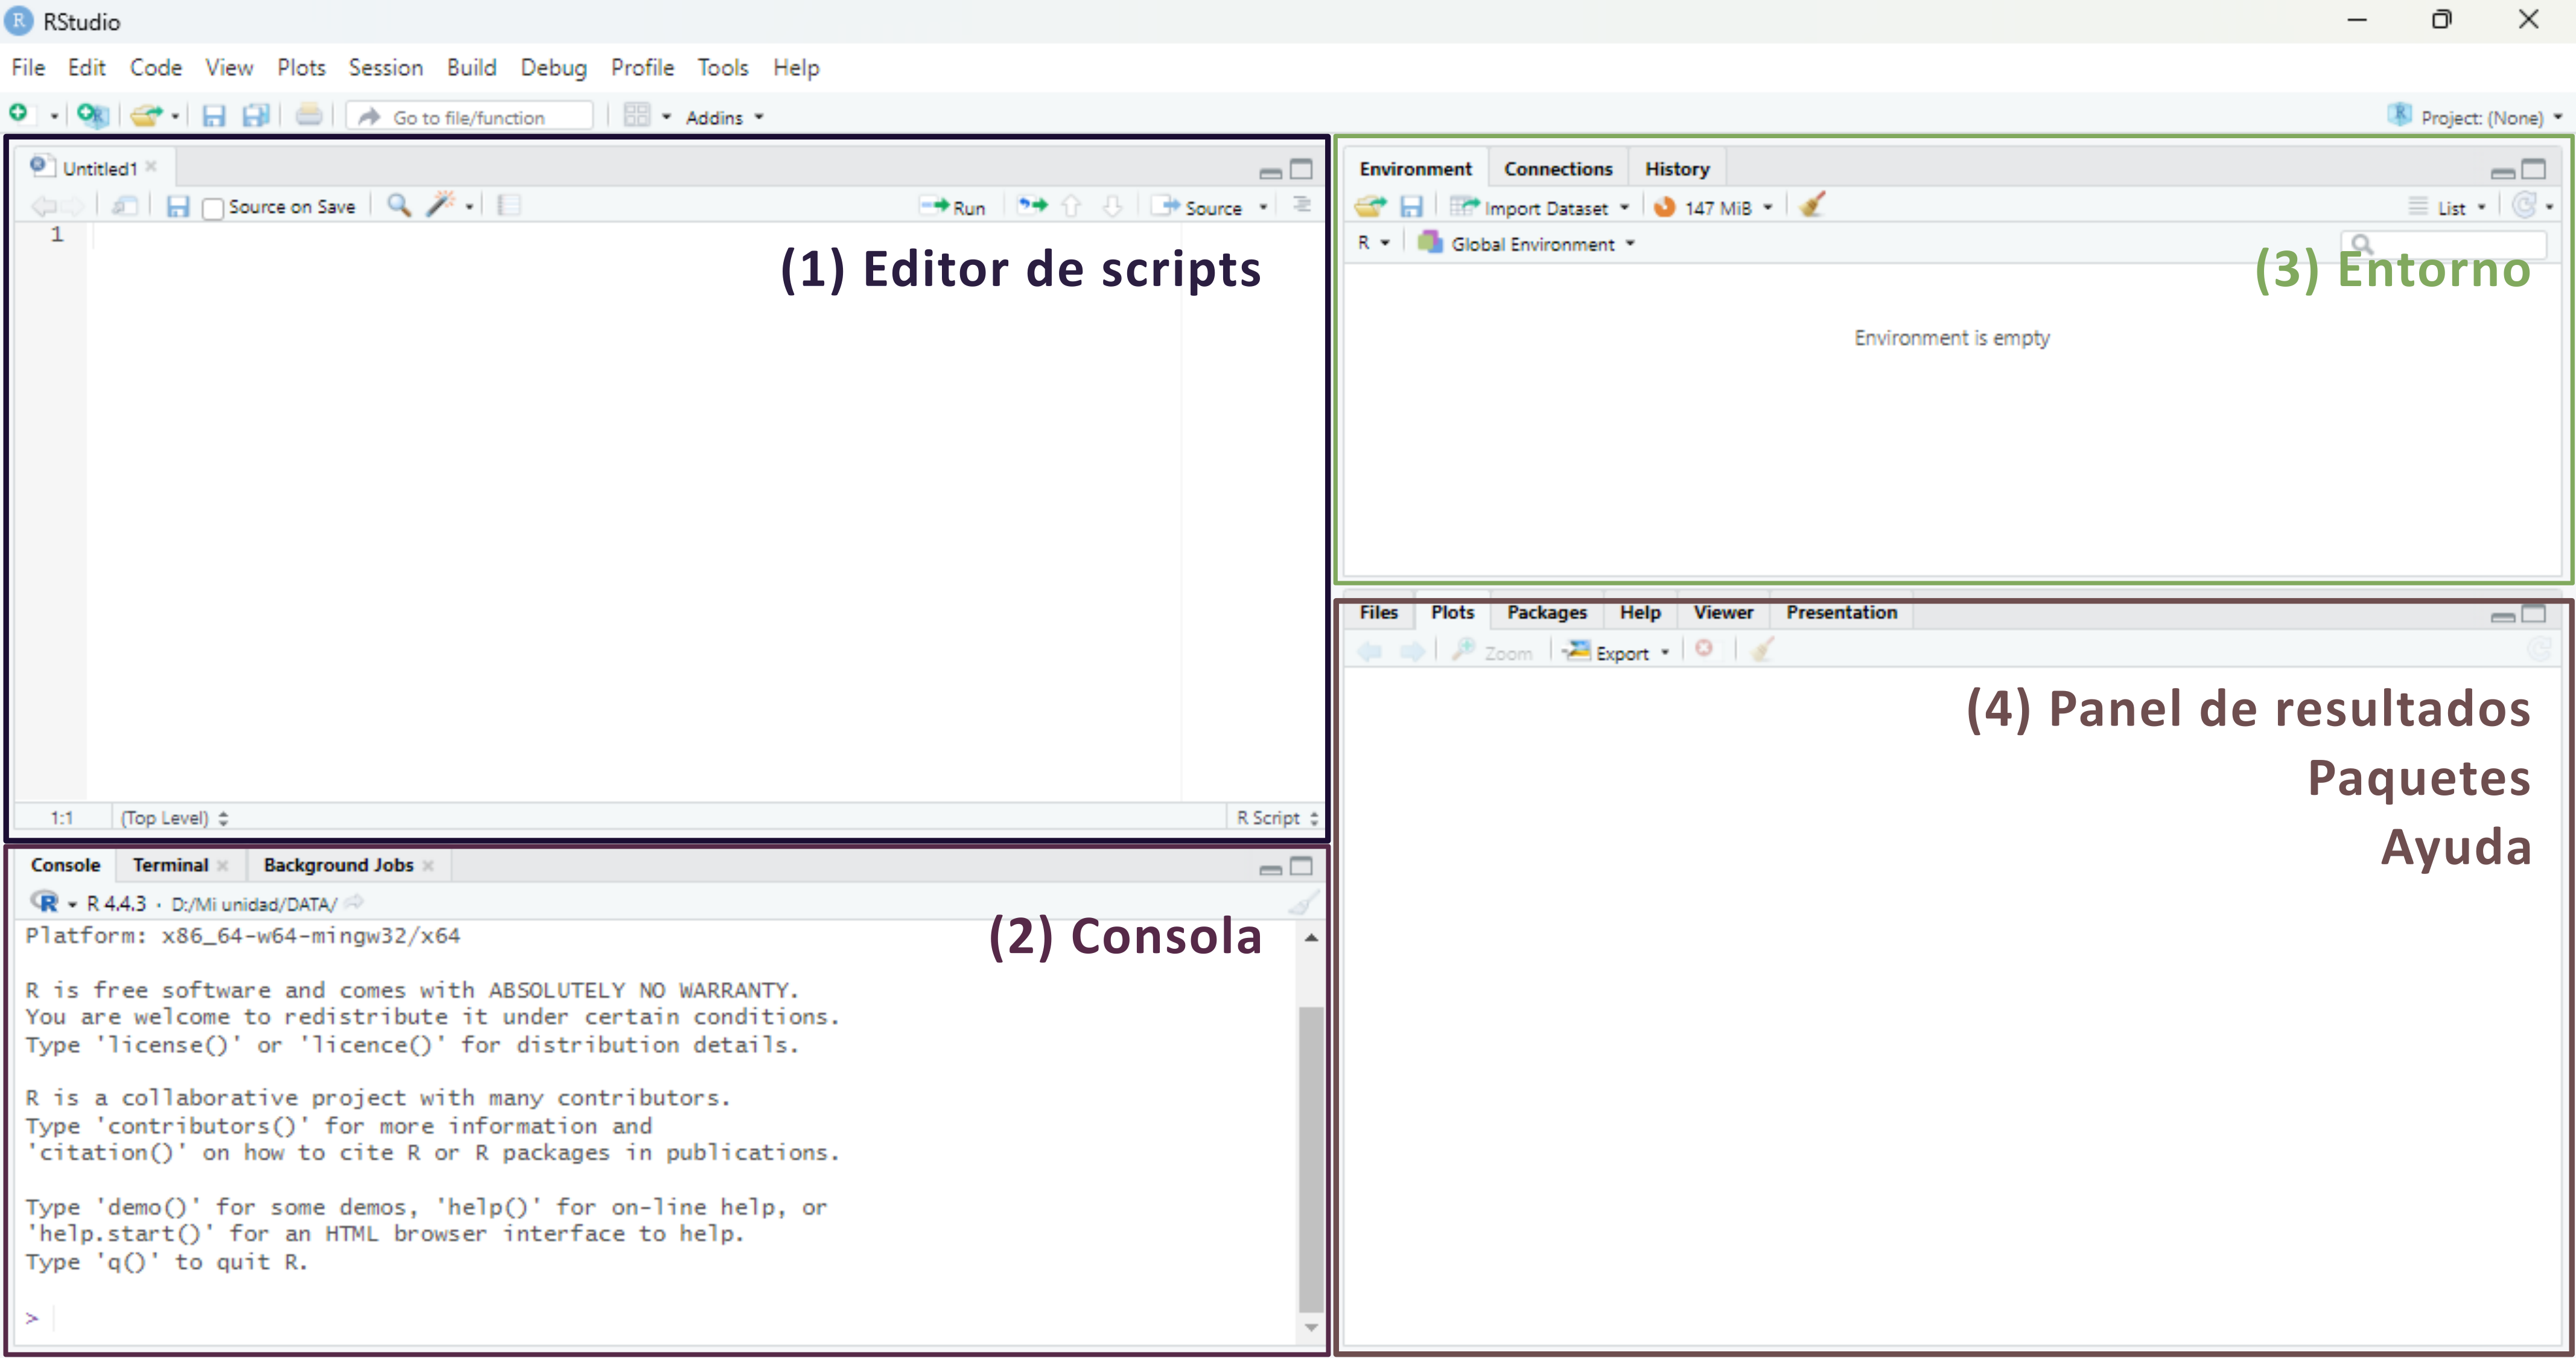
\includegraphics[width=0.95\linewidth,height=\textheight,keepaspectratio]{unidad_1/images/rstudio.png}
\end{center}

\begin{enumerate}
\def\labelenumi{\arabic{enumi}.}
\item
  \textbf{Editor de scripts} (\emph{Source}): permite crear y editar
  scripts de R, así como documentos R Markdown o Quarto.
\item
  \textbf{Consola de R} (\emph{Console}): muestra la salida del código
  ejecutado y ejecuta código de R de forma inmediata.
\item
  \textbf{Entorno} (\emph{Environment}): muestra los objetos creados
  durante la sesión, como vectores, \emph{dataframes} o funciones.
\item
  \textbf{Panel de resultados} (\emph{Output}): presenta los gráficos,
  tablas, visualizaciones en HTML y también incluye un explorador de
  archivos, visor de paquetes instalados y panel de ayuda.
\end{enumerate}

Para garantizar la reproducibilidad de los resultados, es recomendable
evitar el guardado automático del historial de objetos entre sesiones,
ya que puede generar confusión. Para desactivar esta opción, ir a
\texttt{Tools\ \textgreater{}\ Global\ Options} y desmarcar las casillas
de las opciones \textbf{Workspace} y \textbf{History} como se muestra en
la siguiente imagen:

\begin{center}
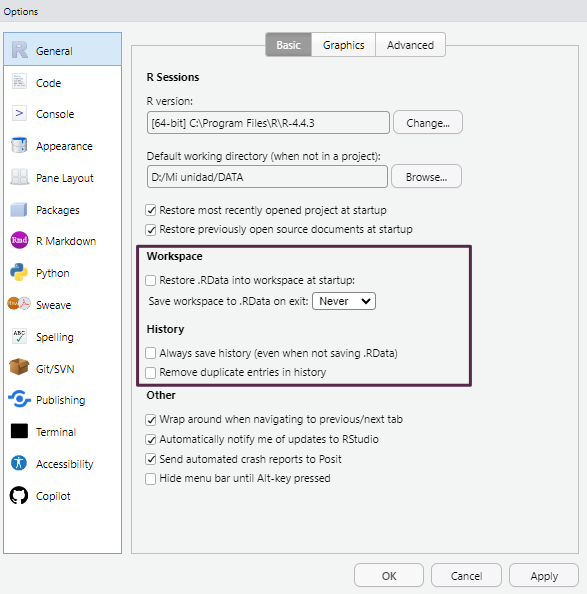
\includegraphics[width=6.25in,height=\textheight,keepaspectratio]{unidad_1/images/global_opts.png}
\end{center}

\section{Proyectos de RStudio}\label{proyectos-de-rstudio}

Los proyectos de RStudio permiten organizar de forma estructurada todo
el material asociado a un análisis: scripts, informes, bases de datos,
imágenes, etc. Cada proyecto se vincula a una carpeta específica del
sistema de archivos, y RStudio la utiliza como directorio de trabajo por
defecto. Esta carpeta puede estar ubicada en cualquier parte del sistema
de almacenamiento que deseemos (disco rígido, pendrive, disco externo,
etc).

Trabajar con proyectos facilita la importación de datos y evita errores
relacionados con rutas relativas o absolutas.

\subsection{Crear un proyecto}\label{crear-un-proyecto}

Para crear un nuevo proyecto, se puede utilizar el menú
\texttt{File\ \textgreater{}\ New\ Project...}. También accedemos a
generar un proyecto nuevo a partir de pulsar el acceso directo
\texttt{New\ Project...} ubicado en la esquina superior derecha de la
interfaz:

\begin{center}
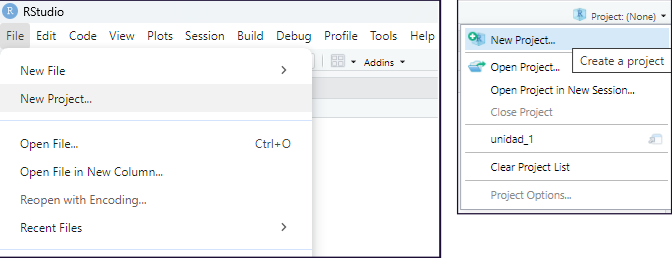
\includegraphics[width=6.25in,height=\textheight,keepaspectratio]{unidad_1/images/proyecto01.png}
\end{center}

En cualquiera de los dos casos aparecerá un cuadro de diálogo que
presenta tres opciones para crear el \textbf{nuevo proyecto} de RStudio:

\begin{center}
\pandocbounded{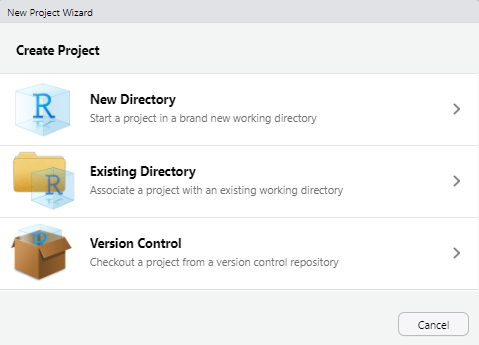
\includegraphics[keepaspectratio]{unidad_1/images/proyecto02.png}}
\end{center}

\begin{itemize}
\item
  \textbf{New Directory}: crea una nueva carpeta para el proyecto a la
  que deberemos asignarle un nombre, es la opción más habitual. Todos
  los archivos de configuración aparecerán asociados a esta nueva
  carpeta.
\item
  \textbf{Existing Directory}: vincula el proyecto a una \emph{carpeta
  ya existente} que contenga archivos previos con los que deseamos
  trabajar.
\item
  \textbf{Version Control}: permite clonar un repositorio (Git o SVN).
  Esta opción no se utilizará durante el curso.
\end{itemize}

Una vez que creamos un nuevo proyecto con la opción \textbf{New
Directory}, aparecerá una pantalla con una lista de tipos de proyectos
que se pueden crear en RStudio:

\begin{center}
\pandocbounded{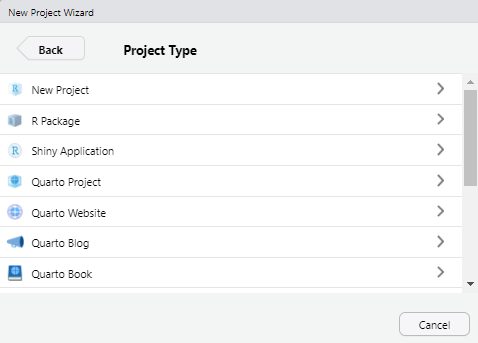
\includegraphics[keepaspectratio]{unidad_1/images/proyecto03.png}}
\end{center}

Durante este curso utilizaremos siempre la \textbf{primera opción}
(\textbf{New Project}). Las demás opciones están pensadas para usos más
específicos, como el desarrollo de paquetes de R, sitios web o
documentos con Quarto o R Markdown.

Al seleccionar \textbf{New Project}, se abrirá una nueva ventana con los
siguientes campos:

\begin{itemize}
\item
  \textbf{Directory name:} aquí debemos escribir el nombre del nuevo
  directorio (carpeta) que también será el nombre del proyecto. Por
  ejemplo, podemos llamarlo \texttt{Practicas\_R}.
\item
  \textbf{Create project as subdirectory of:} este campo permite definir
  en qué ubicación del sistema de archivos se guardará el proyecto.
  Podemos hacer clic en el botón \textbf{Browse\ldots{}} para abrir el
  explorador de archivos y seleccionar la carpeta contenedora. En
  nuestro ejemplo, lo ubicaremos dentro de \textbf{Mis Documentos}.
\end{itemize}

\begin{center}
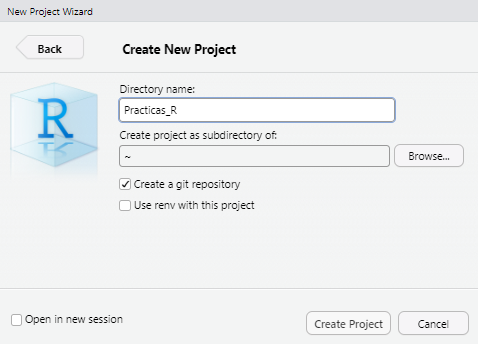
\includegraphics[width=4.98958in,height=\textheight,keepaspectratio]{unidad_1/images/proyecto04.png}
\end{center}

Una vez completados estos campos, hacemos clic en \textbf{Create
Project}.

Los proyectos en RStudio tienen entornos independientes, lo que
significa que si cerramos un proyecto o cambiamos a otro, la
configuración de cada uno se mantendrá inalterable sin interferir con
los demás.

Esto incluye los scripts abiertos, el directorio de trabajo, las
pestañas que dejamos activas y otros elementos del entorno que puedan
ser necesarios para continuar con un análisis. Este sistema permite
mantener organizados los distintos trabajos que llevamos adelante.

Echemos un vistazo a lo que RStudio realizó:

\begin{itemize}
\item
  En primer lugar el panel \textbf{Files} (pantalla inferior derecha)
  apunta a la nueva carpeta \textbf{Practicas\_R} y dentro de ella vemos
  un nuevo archivo el nombre del proyecto y la extensión
  \texttt{.Rproj}. Este archivo contiene todas las configuraciones para
  su proyecto.
\item
  El otro cambio se observa en la parte superior derecha, que muestra el
  nombre del proyecto. Si hacemos click en él, se desplegará el menú de
  proyectos. Desde aquí se puede abrir y cerrar proyectos, navegar
  rápidamente a proyectos que se han abierto recientemente y configurar
  las opciones de RStudio para cada uno de ellos.
\end{itemize}

\begin{center}
\pandocbounded{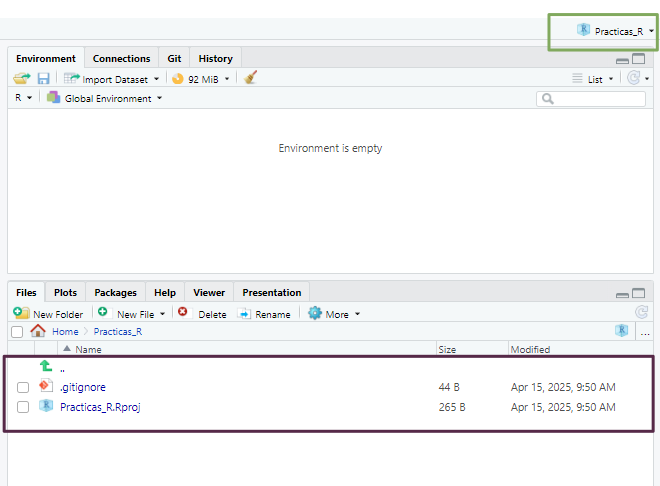
\includegraphics[keepaspectratio]{unidad_1/images/proyecto05.png}}
\end{center}

\subsection{Abrir un proyecto
existente}\label{abrir-un-proyecto-existente}

Cuando el proyecto ya existe, sea porque lo creamos nosotros o porque
alguien nos pasó una carpeta con un proyecto de RStudio creado vamos a
visualizar dentro de esa carpeta un archivo con extensión
\texttt{.Rproj}.

La forma más veloz para abrir el proyecto es ejecutar este archivo
(debería abrir una sesión de RStudio con el proyecto activo). La otra
forma es desde el menú superior derecho de RStudio en la opción
\textbf{Open project\ldots{}} y luego buscando en nuestro directorio el
mismo archivo \texttt{.Rproj}.

\begin{tcolorbox}[enhanced jigsaw, arc=.35mm, bottomrule=.15mm, breakable, colback=white, colframe=quarto-callout-warning-color-frame, left=2mm, leftrule=.75mm, opacityback=0, rightrule=.15mm, toprule=.15mm]

\vspace{-3mm}\textbf{Nota}\vspace{3mm}

El menú de proyectos del área superior derecha va guardando como
elementos recientes los proyectos que se van abriendo y también es una
forma rápida de acceder a ellos pulsando sobre estos atajos.

\end{tcolorbox}

\section{Scripts en RStudio}\label{scripts-en-rstudio}

Como vimos \hyperref[scripts-de-r]{\textbf{anteriormente}}, un script es
un archivo de código que contiene una secuencia de instrucciones
escritas en R. Estos scripts pueden ser reutilizados, modificados y
compartidos, lo que los convierte en una herramienta fundamental para
garantizar la reproducibilidad del trabajo.

\subsection{Crear un nuevo script}\label{crear-un-nuevo-script}

Tenemos varias formas de crear un script nuevo:

\begin{itemize}
\item
  Desde el menú superior:
  \texttt{File\ \textgreater{}\ New\ File\ \textgreater{}\ R\ Script}
\item
  Con el atajo de teclado: \texttt{Ctrl\ +\ Shift\ +\ N}
\item
  Desde la barra de herramientas: presionando el ícono
  \pandocbounded{
\includegraphics[keepaspectratio]{unidad_1/images/script_new.png}}
\end{itemize}

\subsection{Ejecutar scripts}\label{ejecutar-scripts}

La forma habitual de ejecutar el contenido de un script es línea por
línea, usando alguna de las siguientes opciones:

\begin{itemize}
\item
  Presionando el botón
  \pandocbounded{
\includegraphics[keepaspectratio]{unidad_1/images/script_run.png}}
  del editor de código de RStudio
\item
  Mediante el atajo de teclado \texttt{Ctrl\ +\ Enter}
\end{itemize}

Para ejecutar una línea, simplemente ubicamos el cursor en cualquier
parte de ella y presionamos el comando correspondiente. Luego de
ejecutarse, el cursor avanzará automáticamente a la siguiente línea de
código.

Mientras ejecutamos cada línea debemos ir observando la salida en la
consola (panel inferior izquierdo) y también los cambios que se dan en
el panel \emph{Environment} (panel superior derecho) donde aparecerán
los objetos que vayamos creando y manipulando.

\subsection{Edición de scripts}\label{ediciuxf3n-de-scripts}

Modificar o agregar líneas al script puede hacerse directamente en el
editor. Cada vez que realizamos un cambio, es necesario \textbf{volver a
ejecutar la línea} o bloque modificado para que los cambios se reflejen
en el entorno de trabajo.

Podemos probar y modificar tantas veces como sea necesario. Sin embargo,
debemos tener presente que cada manipulación en los objetos se mantiene
hasta que se vuelvan a cambiar y a veces, cuando los objetos están
vinculados con otras líneas de código posteriores tenemos que tener
cuidado que se mantenga la consistencia del script.

Por ejemplo: si definimos un vector numérico para realizar cálculos
matemáticos, pero luego lo sobrescribimos con un valor de tipo caracter,
los cálculos posteriores producirán un error y RStudio nos informará de
esto en la consola.

Por eso, es clave observar el contenido de los objetos en el panel
\textbf{Environment}, lo que nos ayuda a evitar errores y operaciones
incoherentes.

\subsection{Guardado de scripts}\label{guardado-de-scripts}

Cualquier agregado o modificación que hayamos realizado al script y nos
interese mantener nos obligará a guardar el archivo de código editado.

Existen distintas formas de guardar un script:

\begin{itemize}
\item
  Desde el menú superior: \texttt{File\ \textgreater{}\ Save}
\item
  Con el atajo de teclado: \texttt{Ctrl\ +\ S}
\item
  Presionando el ícono del disquete azul 💾
\end{itemize}

Si en cambio quisiera guardarlo como otro archivo para mantener el
script original, podemos guardarlo con diferente nombre o en otra
ubicación mediante \texttt{File\ \textgreater{}\ Save\ As...}

\subsection{Abrir scripts existentes}\label{abrir-scripts-existentes}

Los scripts que construyamos o nos compartan siempre tendrán extensión
\texttt{.R} y, por lo general, se encontrarán dentro de un proyecto.

Para abrir estos archivos \texttt{.R} podemos:

\begin{itemize}
\item
  Desde el menú superior: \texttt{File\ \textgreater{}\ Open\ file...}
\item
  Con el atajo de teclado: \texttt{Ctrl\ +\ O}
\item
  Haciendo click sobre el archivo desde el panel \emph{Files}
\item
  Presionando el botón de la carpeta amarilla 📂
\end{itemize}

Esto abrirá el script en una nueva pestaña dentro del editor de código.

\subsection{¿Cómo trabajaremos en este
curso?}\label{cuxf3mo-trabajaremos-en-este-curso}

En general, utilizaremos scripts dentro de \textbf{proyectos de
RStudio}. La secuencia recomendada será:

\begin{enumerate}
\def\labelenumi{\arabic{enumi}.}
\item
  \textbf{Descargar} desde el Aula Virtual un archivo comprimido
  conteniendo la carpeta, el proyecto, los scripts y archivos de datos.
\item
  \textbf{Descomprimir} el archivo en la ubicación que deseamos
  (recomendamos crear una carpeta destinada al curso).
\item
  Abrir la carpeta y ejecutar el archivo de proyecto \texttt{.Rproj}.
\item
  Una vez abierto RStudio con el proyecto activo, ubicamos los scripts
  desde el panel \textbf{Files}.
\item
  \textbf{Ejecutar} cada línea del script, leyendo la documentación del
  código y observando la salida en la consola y los cambios en el
  entorno
\end{enumerate}

\section{Herramientas de RStudio}\label{herramientas-de-rstudio}

Algunas de las herramientas fundamentales de RStudio son el asistente de
código, la ayuda en línea y el historial de comandos.

\subsection{Asistente de código}\label{asistente-de-cuxf3digo}

Al escribir en el editor o la consola, la tecla \texttt{Tab} activa el
autocompletado de funciones, nombres de objetos y argumentos, agilizando
la escritura y reduciendo errores de sintaxis. En versiones recientes,
el asistente también permite la previsualización de colores en los
gráficos, resaltar los paréntesis de cierre en funciones anidadas con
distintos colores y gestionar automáticamente la indentación del código.

\begin{center}
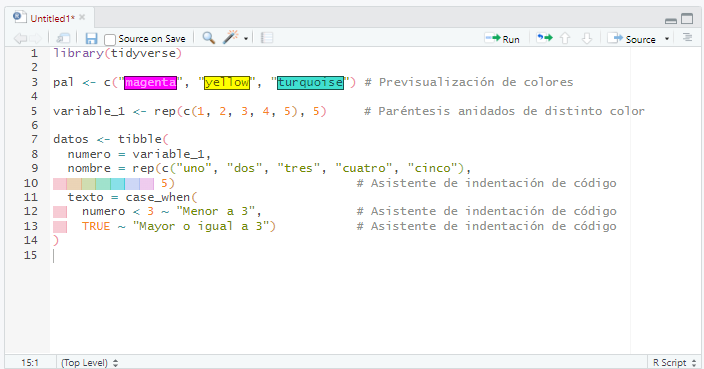
\includegraphics[width=6.25in,height=\textheight,keepaspectratio]{unidad_1/images/asistente.png}
\end{center}

Muchas de estas opciones se pueden configurar desde el menú
\texttt{Code} y desde
\texttt{Tools\ \textgreater{}\ Global\ Options\ \textgreater{}\ Code}(pestañas
\textbf{Editing} y \textbf{Display}).

\begin{center}
\pandocbounded{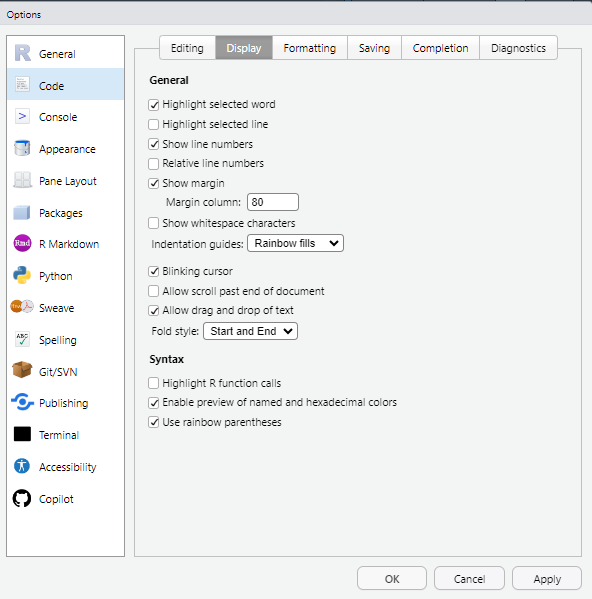
\includegraphics[keepaspectratio]{unidad_1/images/code_display.png}}
\end{center}

\subsection{Ayuda en línea}\label{ayuda-en-luxednea}

Al posicionar el cursor sobre el nombre de una función en el editor y
presionar \texttt{F1}, se accede directamente a la documentación
correspondiente en el panel \textbf{Help} (habitualmente ubicado en la
esquina inferior derecha).

\begin{center}
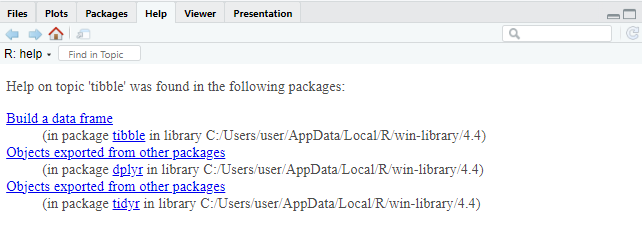
\includegraphics[width=6.25in,height=\textheight,keepaspectratio]{unidad_1/images/help.png}
\end{center}

\subsection{Historial de comandos}\label{historial-de-comandos}

En la consola, al usar las teclas de flecha arriba/abajo, se puede
navegar por los comandos ejecutados durante la sesión actual. Además, el
panel \textbf{History} (parte superior derecha) almacena los comandos de
todas las sesiones previas, permitiendo reutilizarlos con un clic en
\textbf{To Console} (\texttt{Enter}) o \textbf{To Source}
(\texttt{Shift\ +\ Enter}), según se desee insertarlos en la consola o
en el script activo.

\begin{center}
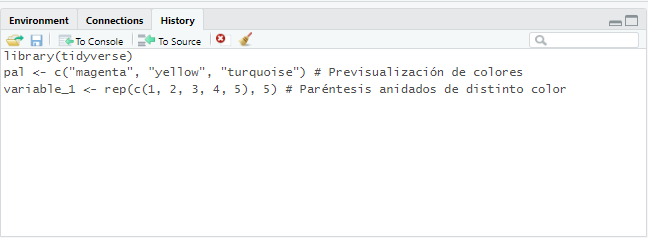
\includegraphics[width=6.25in,height=\textheight,keepaspectratio]{unidad_1/images/historial.png}
\end{center}

\section{Atajos de teclado (Windows)}\label{atajos-de-teclado-windows}

{\def\LTcaptype{none} % do not increment counter
\begin{longtable}[]{@{}
  >{\raggedright\arraybackslash}p{(\linewidth - 2\tabcolsep) * \real{0.2283}}
  >{\raggedright\arraybackslash}p{(\linewidth - 2\tabcolsep) * \real{0.7717}}@{}}
\toprule\noalign{}
\begin{minipage}[b]{\linewidth}\raggedright
Menú
\end{minipage} & \begin{minipage}[b]{\linewidth}\raggedright
Descripción
\end{minipage} \\
\midrule\noalign{}
\endhead
\bottomrule\noalign{}
\endlastfoot
Archivo (File) & \\
Ctrl + Shift + N & Crea un nuevo script \\
Ctrl + O & Abre un script guardado \\
Ctrl + S & Guarda el script activo \\
Ctrl + W & Cierra el script activo \\
Ctrl + Q & Sale del programa RStudio \\
Edición (Edit) & \\
Ctrl + F & Abre la ventana de búsqueda (para buscar palabras dentro de
un script) \\
Ctrl + L & Limpia la consola \\
Código (Code) & \\
Ctrl + Enter & Ejecuta la línea de código donde está situado el
cursor \\
Ctrl + Alt + R & Ejecuta todo el código del script activo \\
Ctrl + Shift + N & Inserta nueva sección de código \\
Ctrl + Shift + R & Inserta nueva sección de comentarios de texto \\
Sesión (Session) & \\
Ctrl + Shift + H & Abre la ventana para establecer directorio de
trabajo \\
Ctrl + Shift + F10 & Reinicia la sesión de R \\
Herramientas (Tools) & \\
Alt + Shift + K & Abre la lista de ayuda de atajos de teclado \\
\end{longtable}
}

\section{Paquetes}\label{paquetes}

Existen dos formas principales de descargar paquetes: directamente desde
RStudio o desde el
\href{https://cran.r-project.org/web/packages/}{\textbf{sitio web de
CRAN}}, descargándolos como archivos comprimidos. Si el equipo cuenta
con conexión a Internet, lo más práctico es realizar la descarga
directamente desde RStudio. En cambio, si no se dispone de acceso
permanente a la red, es posible descargar los paquetes desde otro equipo
y luego transferirlos como archivos \texttt{.zip} o \texttt{.tar.gz} al
equipo donde se encuentra instalado R.

Cuando accedemos al sitio web de CRAN y buscamos un paquete específico,
encontraremos información útil como una breve descripción del paquete,
el número de versión, la fecha de publicación, el nombre del autor,
documentación asociada y enlaces de descarga específicos para cada
sistema operativo.

Dado que la mayoría de las computadoras hoy en día cuentan con acceso a
Internet, en este curso nos enfocaremos en la instalación y activación
de paquetes directamente desde RStudio.

Dentro del entorno de RStudio, la gestión de paquetes se realiza desde
la pestaña \emph{Packages}, ubicada en el panel inferior derecho. Esta
interfaz facilita tareas como la instalación, actualización y activación
de paquetes, y cada acción que realizamos desde la interfaz gráfica se
traduce internamente en la ejecución de funciones del lenguaje R que
pueden observarse en la consola.

Para instalar un paquete nuevo, simplemente pulsamos el botón
\emph{Install} dentro de la pestaña \emph{Packages}, lo cual abrirá una
ventana emergente.

\begin{center}
\pandocbounded{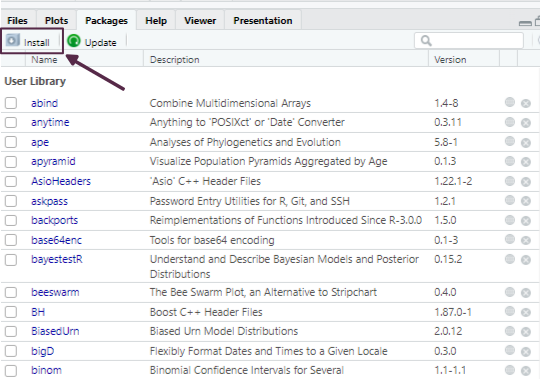
\includegraphics[keepaspectratio]{unidad_1/images/rstudio_paquetes01.png}}
\end{center}

Allí podemos escribir el nombre del paquete que deseamos instalar. Para
asegurarnos de que también se descarguen e instalen automáticamente los
paquetes de los que depende, es importante tildar la opción
\emph{Install dependencies}.

\begin{center}
\pandocbounded{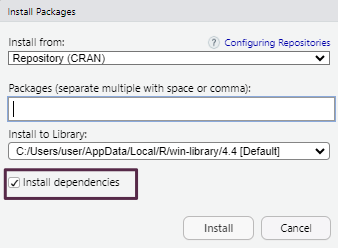
\includegraphics[keepaspectratio]{unidad_1/images/rstudio_paquetes02.png}}
\end{center}

Como alternativa, también podemos realizar la instalación desde el
editor de scripts mediante el siguiente comando:

\begin{Shaded}
\begin{Highlighting}[]
\FunctionTok{install.packages}\NormalTok{(}\StringTok{"nombre\_del\_paquete"}\NormalTok{, }\AttributeTok{dependencies =} \ConstantTok{TRUE}\NormalTok{)}
\end{Highlighting}
\end{Shaded}

\begin{tcolorbox}[enhanced jigsaw, arc=.35mm, bottomrule=.15mm, breakable, colback=white, colframe=quarto-callout-note-color-frame, left=2mm, leftrule=.75mm, opacityback=0, rightrule=.15mm, toprule=.15mm]

Para facilitar la instalación de los paquetes requeridos durante el
curso, recomendamos descargar el archivo
\textbf{``\href{../files/datos_y_paquetes.zip}{Paquetes y datos para el
curso}''}, descomprimirlo y ejecutar el script que se encuentra en su
interior.

\end{tcolorbox}

\section{Lectura de archivos de
datos}\label{lectura-de-archivos-de-datos}

R permite importar tablas de datos desde diversos formatos, tanto
utilizando funciones de \textbf{R base} como funciones provistas por
paquetes específicos.

El formato más común es el \textbf{texto plano} (ASCII), donde los
valores están organizados en columnas separadas por caracteres
delimitadores. Los separadores más habituales incluyen:

\begin{itemize}
\item
  Coma (\texttt{,})
\item
  Punto y coma (\texttt{;})
\item
  Tabulación (\texttt{\textbackslash{}t})
\item
  Barra vertical (\texttt{\textbar{}})
\end{itemize}

Estos archivos suelen tener una \textbf{cabecera} (\emph{header}) en la
primera fila con los nombres de las variables, y cada columna debe
contener datos del mismo tipo (números, texto, lógicos, etc.).

Para importar correctamente un archivo es importante conocer su
estructura:

\begin{itemize}
\item
  Si incluye o no cabecera.
\item
  Qué carácter se usa como separador.
\item
  El tipo de codificación (UTF-8, Latin1, etc.).
\end{itemize}

Dado que son archivos de texto, pueden visualizarse con editores simples
como el Bloc de Notas o desde RStudio, lo que facilita su inspección
previa.

Para cargar los datos desde un archivo de texto plano usamos el código:

\begin{Shaded}
\begin{Highlighting}[]
\NormalTok{datos }\OtherTok{\textless{}{-}} \FunctionTok{read.xxx}\NormalTok{(}\StringTok{"mis\_datos.xxx"}\NormalTok{)}
\end{Highlighting}
\end{Shaded}

(Se debe reemplazar \texttt{read.xxx()} por la función correspondiente:
\texttt{read.table()}, \texttt{read.csv()}, \texttt{read\_delim()},
\texttt{read\_excel()}, etc., según la extensión del archivo).

R también permite cargar bases de datos incluidas en paquetes instalados
mediante:

\begin{Shaded}
\begin{Highlighting}[]
\FunctionTok{data}\NormalTok{(nombre\_datos)}

\NormalTok{datos }\OtherTok{\textless{}{-}}\NormalTok{ nombre\_datos}
\end{Highlighting}
\end{Shaded}

\section{Buenas prácticas}\label{buenas-pruxe1cticas}

Adoptar buenas prácticas desde el inicio mejora la reproducibilidad,
facilita el trabajo colaborativo y reduce errores. Algunas
recomendaciones clave son:

\begin{itemize}
\item
  Trabajar \textbf{siempre} dentro de un \textbf{proyecto de RStudio}
  (\texttt{.Rproj}). Esto permite organizar los archivos, mantener rutas
  relativas consistentes y acceder a funcionalidades específicas como
  control de versiones o panel de archivos integrados.
\item
  Incluir al comienzo de cada script las líneas de \textbf{activación de
  paquetes} necesarios, utilizando la función \texttt{library()}.
\item
  \textbf{Cargar los datos} una vez activados los paquetes, para
  garantizar que todas las funciones requeridas estén disponibles.
\item
  Documentar el código mediante \textbf{comentarios} iniciados con
  \texttt{\#}. Esto permite entender qué hace cada bloque de código,
  facilitando futuras modificaciones o revisiones.
\item
  \textbf{Usar espacios e indentación adecuada} para mejorar la
  legibilidad. Esto es especialmente importante en estructuras anidadas
  (como condicionales, bucles o funciones).
\end{itemize}

\chapter{\texorpdfstring{Introducción a
\texttt{tidyverse}}{Introducción a tidyverse}}\label{introducciuxf3n-a-tidyverse}

\begin{center}

\includegraphics[width=0.44\linewidth,height=\textheight,keepaspectratio]{bg_images/tidyverse.png}
\end{center}

\section{Introducción}\label{introducciuxf3n}

Tidyverse es el nombre que recibe el conjunto de paquetes desarrollados
y/o promovidos por
\href{https://en.wikipedia.org/wiki/Hadley_Wickham}{\textbf{Hadley
Wickham}} (jefe científico en Posit/RStudio) y su equipo, orientado al
trabajo de ciencia de datos con R (Wickham et~al. 2019). Estos paquetes
están diseñados para integrarse de manera coherente, compartiendo una
misma filosofía de diseño conocida como
\href{https://cran.r-project.org/web/packages/tidyverse/vignettes/manifesto.html}{\textbf{\emph{The
tidy tools manifesto}}}.

Los cuatro principios básicos sobre los que se construye
\emph{tidyverse} son:

\begin{itemize}
\item
  Reutilización de estructuras de datos
\item
  Resolución de problemas complejos combinando varias piezas sencillas
\item
  Uso de programación funcional
\item
  Diseño orientado a las personas
\end{itemize}

Los paquetes incluidos cubren todas las etapas del análisis de datos
dentro de R: importación y ordenamiento de los datos (\emph{tidy data}),
transformación, visualización, modelado y la posterior comunicación de
resultados.

La palabra \emph{tidy} se traduce como ``ordenado'', y hace referencia a
una estructura específica que deben cumplir los datos:

\begin{itemize}
\tightlist
\item
  Cada \textbf{\emph{variable}} es una \emph{columna} de la tabla de
  datos.
\item
  Cada \textbf{\emph{observación}} es una \emph{fila} de la tabla de
  datos.
\item
  Cada \textbf{\emph{tabla}} responde a una \emph{unidad de observación
  o} análisis.
\end{itemize}

\begin{center}
\pandocbounded{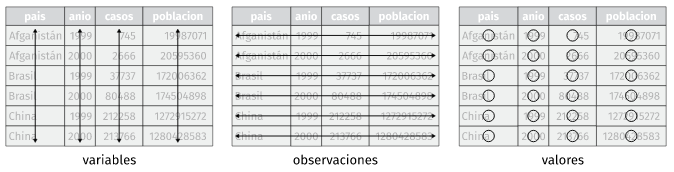
\includegraphics[keepaspectratio]{unidad_1/images/tidy.PNG}}
\end{center}

Además de los paquetes principales, al instalar \texttt{tidyverse} se
incluyen otros que permiten trabajar con fechas, cadenas de caracteres o
factores, también siguiendo los mismos principios.

Uno de los objetivos de los desarrolladores fue dotar a la sintaxis de
estos paquetes de una \textbf{gramática} clara: funciones cuyos nombres
y argumentos permiten construir ``\emph{frases}'' que sean
semánticamente comprensibles. Un ejemplo de esto se ve en el paquete
\texttt{dplyr}, donde la mayoría de las funciones son verbos en inglés
como \texttt{filter()}, \texttt{mutate()}, \texttt{summarise()}, lo que
facilita su lectura y comprensión.

El paquete \texttt{tidyverse} puede instalarse desde el repositorio
oficial CRAN mediante el menú \emph{Packages} de RStudio, o ejecutando
el siguiente código:

\begin{Shaded}
\begin{Highlighting}[]
\FunctionTok{install.packages}\NormalTok{(}\StringTok{"tidyverse"}\NormalTok{)}
\end{Highlighting}
\end{Shaded}

Una vez instalado, se activa mediante:

\begin{Shaded}
\begin{Highlighting}[]
\FunctionTok{library}\NormalTok{(tidyverse)}
\end{Highlighting}
\end{Shaded}

Al activarlo, se muestra un mensaje con la versión instalada, la lista
de paquetes que se cargan automáticamente y posibles conflictos de
nombres entre funciones. Esto es habitual cuando se utilizan múltiples
paquetes, ya que algunas funciones pueden llamarse igual. Por ejemplo,
la función \texttt{filter()} existe tanto en el paquete \texttt{stats}
como en \texttt{dplyr}. Al cargar \texttt{tidyverse}, R avisa de esta
superposición:

\texttt{✖️dplyr::filter()\ masks\ stats::filter()}

Cuando necesitamos asegurarnos de que estamos usando la función de un
paquete específico, se recomienda usar la notación \texttt{::}, por
ejemplo:

\begin{Shaded}
\begin{Highlighting}[]
\CommentTok{\# Función filter() del paquete stats}
\NormalTok{stats}\SpecialCharTok{::}\FunctionTok{filter}\NormalTok{()}

\CommentTok{\# Función filter() del paquete tidyverse}
\NormalTok{dplyr}\SpecialCharTok{::}\FunctionTok{filter}\NormalTok{()}
\end{Highlighting}
\end{Shaded}

Una estrategia útil cuando trabajamos con varios paquetes es cargar
\texttt{tidyverse} al final de la lista de paquetes, para que sus
funciones sobrescriban las de otros paquetes si fuese necesario:

\begin{Shaded}
\begin{Highlighting}[]
\FunctionTok{library}\NormalTok{(stats)}
\FunctionTok{library}\NormalTok{(tidyverse)}
\end{Highlighting}
\end{Shaded}

Los paquetes que se instalan con la versión actual de \texttt{tidyverse}
pueden consultarse ejecutando:

\begin{Shaded}
\begin{Highlighting}[]
\FunctionTok{tidyverse\_packages}\NormalTok{()}
\end{Highlighting}
\end{Shaded}

\begin{verbatim}
 [1] "broom"         "conflicted"    "cli"           "dbplyr"       
 [5] "dplyr"         "dtplyr"        "forcats"       "ggplot2"      
 [9] "googledrive"   "googlesheets4" "haven"         "hms"          
[13] "httr"          "jsonlite"      "lubridate"     "magrittr"     
[17] "modelr"        "pillar"        "purrr"         "ragg"         
[21] "readr"         "readxl"        "reprex"        "rlang"        
[25] "rstudioapi"    "rvest"         "stringr"       "tibble"       
[29] "tidyr"         "xml2"          "tidyverse"    
\end{verbatim}

Además, existen muchos otros paquetes que siguen la misma filosofía pero
no están incluidos por defecto. En esos casos, deben instalarse y
activarse individualmente.

\begin{tcolorbox}[enhanced jigsaw, arc=.35mm, bottomrule=.15mm, breakable, colback=white, colframe=quarto-callout-warning-color-frame, left=2mm, leftrule=.75mm, opacityback=0, rightrule=.15mm, toprule=.15mm]
\begin{minipage}[t]{5.5mm}
\textcolor{quarto-callout-warning-color}{\faExclamationTriangle}
\end{minipage}%
\begin{minipage}[t]{\textwidth - 5.5mm}

Para profundizar el uso de \texttt{tidyverse}, se recomienda consultar:

Sitio oficial: https://www.tidyverse.org/

Libro \emph{R para Ciencia de Datos}: https://es.r4ds.hadley.nz/

Nueva versión (\emph{r4ds 2e}): https://r4ds.hadley.nz/

EpiRhandbook en español: https://www.epirhandbook.com/es/index.es.html

\end{minipage}%
\end{tcolorbox}

\begin{center}

\includegraphics[width=0.25\linewidth,height=\textheight,keepaspectratio]{bg_images/tibble.png}
\end{center}

\section{\texorpdfstring{\emph{Dataframes} con
\texttt{tibble}}{Dataframes con tibble}}\label{dataframes-con-tibble}

Uno de los paquetes que forman parte del núcleo básico de
\emph{tidyverse} es \texttt{tibble} (Müller y Wickham 2026), que
introduce una versión moderna del objeto \texttt{data.frame}. Todas las
funciones que generan tablas de datos en \emph{tidyverse} devuelven
objetos \emph{tibble} (\texttt{tbl\_df}), los cuales son más eficientes
y amigables para el flujo de trabajo.

Las principales ventajas de trabajar con \texttt{tibble} son:

\begin{itemize}
\item
  Impresión en consola más legible y controlada (muestran un número
  limitado de filas y columnas).
\item
  No cambian automáticamente el tipo de datos.
\item
  Permiten nombres de columnas con espacios o caracteres especiales si
  se encierran entre comillas invertidas \texttt{\textasciigrave{}}
  (aunque \textbf{no se recomienda}).
\end{itemize}

Para crear un objeto \emph{tibble} manualmente usamos el siguiente
código:

\begin{Shaded}
\begin{Highlighting}[]
\NormalTok{datos }\OtherTok{\textless{}{-}} \FunctionTok{tibble}\NormalTok{(}
  \AttributeTok{nombre =} \FunctionTok{c}\NormalTok{(}\StringTok{"Ana"}\NormalTok{, }\StringTok{"Luis"}\NormalTok{, }\StringTok{"María"}\NormalTok{),}
  \AttributeTok{edad =} \FunctionTok{c}\NormalTok{(}\DecValTok{34}\NormalTok{, }\DecValTok{28}\NormalTok{, }\DecValTok{45}\NormalTok{),}
  \AttributeTok{altura =} \FunctionTok{c}\NormalTok{(}\FloatTok{1.65}\NormalTok{, }\FloatTok{1.80}\NormalTok{, }\FloatTok{1.70}\NormalTok{)}
\NormalTok{)}
\end{Highlighting}
\end{Shaded}

\begin{center}

\includegraphics[width=0.25\linewidth,height=\textheight,keepaspectratio]{bg_images/magrittr.png}
\end{center}

\section{\texorpdfstring{Tuberías con
\texttt{magrittr}}{Tuberías con magrittr}}\label{tuberuxedas-con-magrittr}

Una de las incorporaciones más útiles y transversales del ecosistema
\emph{tidyverse} es el uso de ``\emph{tuberías''} o \emph{pipe
operators}. Una tubería conecta un bloque de código con otro,
permitiendo encadenar operaciones de manera legible. El operador
\texttt{\%\textgreater{}\%}, proveniente del paquete \texttt{magrittr}
(Bache y Wickham 2026), transforma llamadas de funciones anidadas (con
múltiples paréntesis) en una secuencia de pasos más simple de leer y
escribir.

A partir de la versión 4.1.0 de R, también se incorporó una
\textbf{tubería nativa} (\texttt{\textbar{}\textgreater{}}), con un
comportamiento muy similar. Ambas opciones son válidas y su uso es
prácticamente equivalente.

Este enfoque refleja el principio de que \emph{cada función representa
un paso en una secuencia lógica de transformación de datos}. La forma de
trabajar se puede ver en el siguiente esquema general:

\begin{center}
\pandocbounded{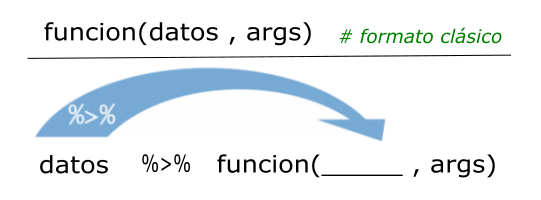
\includegraphics[keepaspectratio]{unidad_1/images/pipe.png}}
\end{center}

A continuación, mostramos un ejemplo comparativo de cómo cambia la
sintaxis usando el dataset incorporado en R \texttt{mtcars}, que
contiene datos sobre autos:

\begin{Shaded}
\begin{Highlighting}[]
\FunctionTok{head}\NormalTok{(}\FunctionTok{sqrt}\NormalTok{(mtcars))}
\end{Highlighting}
\end{Shaded}

\begin{verbatim}
                       mpg      cyl     disp        hp     drat       wt
Mazda RX4         4.582576 2.449490 12.64911 10.488088 1.974842 1.618641
Mazda RX4 Wag     4.582576 2.449490 12.64911 10.488088 1.974842 1.695582
Datsun 710        4.774935 2.000000 10.39230  9.643651 1.962142 1.523155
Hornet 4 Drive    4.626013 2.449490 16.06238 10.488088 1.754993 1.793042
Hornet Sportabout 4.324350 2.828427 18.97367 13.228757 1.774824 1.854724
Valiant           4.254409 2.449490 15.00000 10.246951 1.661325 1.860108
                      qsec vs am     gear     carb
Mazda RX4         4.057093  0  1 2.000000 2.000000
Mazda RX4 Wag     4.125530  0  1 2.000000 2.000000
Datsun 710        4.313931  1  1 2.000000 1.000000
Hornet 4 Drive    4.409082  1  0 1.732051 1.000000
Hornet Sportabout 4.125530  0  0 1.732051 1.414214
Valiant           4.496665  1  0 1.732051 1.000000
\end{verbatim}

En la línea de código anterior estamos pidiendo mostrar la cabecera (6
primeras observaciones de la tabla de datos) de la raíz cuadrada de los
valores de la tabla \texttt{mtcars}, en formato del lenguaje clásico
(anidado).

Ahora activamos \texttt{magrittr} y ejecutamos la línea anterior en
formato tubería:

\begin{Shaded}
\begin{Highlighting}[]
\CommentTok{\# Activa paquete}
\FunctionTok{library}\NormalTok{(magrittr)}

\CommentTok{\# Formato tubería}
\NormalTok{mtcars }\SpecialCharTok{\%\textgreater{}\%}
  \FunctionTok{sqrt}\NormalTok{() }\SpecialCharTok{\%\textgreater{}\%}
  \FunctionTok{head}\NormalTok{()}
\end{Highlighting}
\end{Shaded}

\begin{verbatim}
                       mpg      cyl     disp        hp     drat       wt
Mazda RX4         4.582576 2.449490 12.64911 10.488088 1.974842 1.618641
Mazda RX4 Wag     4.582576 2.449490 12.64911 10.488088 1.974842 1.695582
Datsun 710        4.774935 2.000000 10.39230  9.643651 1.962142 1.523155
Hornet 4 Drive    4.626013 2.449490 16.06238 10.488088 1.754993 1.793042
Hornet Sportabout 4.324350 2.828427 18.97367 13.228757 1.774824 1.854724
Valiant           4.254409 2.449490 15.00000 10.246951 1.661325 1.860108
                      qsec vs am     gear     carb
Mazda RX4         4.057093  0  1 2.000000 2.000000
Mazda RX4 Wag     4.125530  0  1 2.000000 2.000000
Datsun 710        4.313931  1  1 2.000000 1.000000
Hornet 4 Drive    4.409082  1  0 1.732051 1.000000
Hornet Sportabout 4.125530  0  0 1.732051 1.414214
Valiant           4.496665  1  0 1.732051 1.000000
\end{verbatim}

Podemos hacer lo mismo con la tubería nativa de R sin activar ningún
paquete (revisar que esté activada desde
\texttt{Tools\ \textgreater{}\ Global\ Options}):

\begin{Shaded}
\begin{Highlighting}[]
\CommentTok{\# Tubería nativa}
\NormalTok{mtcars }\SpecialCharTok{|\textgreater{}}
  \FunctionTok{sqrt}\NormalTok{() }\SpecialCharTok{|\textgreater{}}
  \FunctionTok{head}\NormalTok{()}
\end{Highlighting}
\end{Shaded}

\begin{verbatim}
                       mpg      cyl     disp        hp     drat       wt
Mazda RX4         4.582576 2.449490 12.64911 10.488088 1.974842 1.618641
Mazda RX4 Wag     4.582576 2.449490 12.64911 10.488088 1.974842 1.695582
Datsun 710        4.774935 2.000000 10.39230  9.643651 1.962142 1.523155
Hornet 4 Drive    4.626013 2.449490 16.06238 10.488088 1.754993 1.793042
Hornet Sportabout 4.324350 2.828427 18.97367 13.228757 1.774824 1.854724
Valiant           4.254409 2.449490 15.00000 10.246951 1.661325 1.860108
                      qsec vs am     gear     carb
Mazda RX4         4.057093  0  1 2.000000 2.000000
Mazda RX4 Wag     4.125530  0  1 2.000000 2.000000
Datsun 710        4.313931  1  1 2.000000 1.000000
Hornet 4 Drive    4.409082  1  0 1.732051 1.000000
Hornet Sportabout 4.125530  0  0 1.732051 1.414214
Valiant           4.496665  1  0 1.732051 1.000000
\end{verbatim}

Las tuberías le dan mucha mas claridad al código separándolo en partes,
como si fuesen oraciones de un párrafo.

\begin{center}

\includegraphics[width=0.25\linewidth,height=\textheight,keepaspectratio]{bg_images/readr.png}
\end{center}

\section{\texorpdfstring{Archivos de texto plano con
\texttt{readr}}{Archivos de texto plano con readr}}\label{archivos-de-texto-plano-con-readr}

El paquete \texttt{readr} (Wickham, Hester, et~al. 2026) contiene
funciones similares a las de la familia \texttt{read.table()} de R base,
pero desarrollados bajo el ecosistema \texttt{tidyverse}.

Los archivos de texto plano (ASCII u otras codificaciones) son
universalmente utilizados por la mayoría de los gestores de bases de
datos y planillas de cálculo. Generalmente se encuentran con extensiones
\texttt{.txt} o \texttt{.csv} (por \emph{comma-separated values}) y son
el tipo de archivo de datos más habitual en R.

Estos datos planos tienen dos características principales:

\begin{itemize}
\tightlist
\item
  La cabecera (en inglés \emph{header}).
\item
  El carácter o símbolo separador que indica la separación de columnas:
  pueden estar separadas por comas, punto y coma, tabulación, etc.
\end{itemize}

La presencia o no de una cabecera se maneja con los argumentos
\texttt{col\_names} y \texttt{skip}:

\begin{itemize}
\item
  \texttt{col\_names\ =\ TRUE} indica que la primera fila contiene los
  nombres de las columnas (cabecera).
\item
  \texttt{col\_names\ =\ FALSE} indica que no hay cabecera y las
  columnas se nombran automáticamente (\texttt{X1}, \texttt{X2}, etc).
\item
  \texttt{skip\ =\ 0} (valor por defecto) lee los datos desde la primera
  fila, pero si hay encabezados complejos (por ejemplo, títulos y
  subtítulos ), se puede indicar cuántas filas deben omitirse. Ejemplo:
  \texttt{skip\ =\ 5} omite las primeras 5 filas del archivo.
\end{itemize}

Otro aspecto a considerar es el carácter \textbf{separador} utilizado
para indicar la separación entre columnas. Los separadores más comunes
son:

\begin{itemize}
\item
  coma (\texttt{,})
\item
  punto y coma (\texttt{;})
\item
  tabulación (\texttt{TAB})
\item
  espacio (\texttt{"\ "})
\item
  barra vertical o \emph{pipe} (\texttt{\textbar{}})
\end{itemize}

\subsubsection{Funciones de lectura}\label{funciones-de-lectura}

Algunas de las funciones del paquete asumen un separador particular. Por
caso \texttt{read\_csv()} lee separados por coma y \texttt{read\_tsv()}
separado por tabulaciones, pero la función \texttt{read\_delim()}
permite que definamos el separador a través del argumento
\texttt{delim}.

En forma detallada el paquete \texttt{readr} soporta siete formatos de
archivo a partir de siete funciones:

\begin{itemize}
\tightlist
\item
  \texttt{read\_csv()}: archivos separados por comas (CSV).
\item
  \texttt{read\_tsv()}: archivos separados por tabulaciones.
\item
  \texttt{read\_delim()}: archivos separados con delimitadores
  generales.
\item
  \texttt{read\_fwf()}: archivos con columnas de ancho fijo.
\item
  \texttt{read\_table()}: archivos formato tabla con columnas separadas
  por espacios.
\item
  \texttt{read\_log()}: archivos log web.
\end{itemize}

En comparación con las funciones R \texttt{base}, las funciones de
\texttt{readr}:

\begin{itemize}
\item
  Usan un esquema de nombres consistente de parámetros.
\item
  Son más rápidas.
\item
  Analizan eficientemente los formatos de datos comunes (especialmente
  fechas y horas).
\item
  Muestra una barra de progreso para archivos grandes.
\item
  Vienen incluidas dentro de \texttt{tidyverse} pero también pueden
  usarse de forma independiente:
\end{itemize}

\begin{Shaded}
\begin{Highlighting}[]
\FunctionTok{library}\NormalTok{(readr)}
\end{Highlighting}
\end{Shaded}

A modo de ejemplo, leeremos un archivo sin cabecera separado por comas
bajo el nombre \texttt{datos}:

\begin{Shaded}
\begin{Highlighting}[]
\NormalTok{datos }\OtherTok{\textless{}{-}} \FunctionTok{read\_csv}\NormalTok{(}\StringTok{"datos/ejemplo{-}datos.csv"}\NormalTok{, }\AttributeTok{col\_names =}\NormalTok{ F)}
\NormalTok{datos}
\end{Highlighting}
\end{Shaded}

\begin{verbatim}
# A tibble: 4 x 5
     X1 X2       X3       X4    X5        
  <dbl> <chr>    <chr>    <chr> <date>    
1     9 Leone    Fernando M     1958-12-24
2    26 Garcia   Esteban  M     1954-01-21
3    35 Salamone Nicolas  M     1993-06-27
4    48 Gonzalez Viviana  F     1965-06-21
\end{verbatim}

Leemos el mismo archivo con cabecera y separado por punto y comas, bajo
el nombre \texttt{info}:

\begin{Shaded}
\begin{Highlighting}[]
\NormalTok{info }\OtherTok{\textless{}{-}} \FunctionTok{read\_csv2}\NormalTok{(}\StringTok{"datos/ejemplo{-}datos{-}header.csv"}\NormalTok{, }\AttributeTok{col\_names =}\NormalTok{ T)}
\NormalTok{info}
\end{Highlighting}
\end{Shaded}

\begin{verbatim}
# A tibble: 4 x 5
   Iden Apellido Nombre   Sexo  FNac      
  <dbl> <chr>    <chr>    <chr> <date>    
1     9 Leone    Fernando M     1958-12-24
2    26 Garcia   Laura    M     1954-01-21
3    35 Salamone Nicolas  M     1993-06-27
4    48 Gonzalez Viviana  F     1965-06-21
\end{verbatim}

En estos ejemplos:

\begin{itemize}
\item
  \texttt{read\_csv()} espera comas como separador
\item
  \texttt{read\_csv2()} espera punto y coma como separador
\end{itemize}

Al leer un archivo, \texttt{readr} intenta adivinar automáticamente el
tipo de dato de cada columna (\emph{parse}). Si no hay cabecera, los
nombres de columna serán \texttt{X1}, \texttt{X2}, etc.

Podemos inspeccionar la estructura de un \emph{dataframe} con
\texttt{glimpse()}:

\begin{Shaded}
\begin{Highlighting}[]
\FunctionTok{glimpse}\NormalTok{(info)}
\end{Highlighting}
\end{Shaded}

\begin{verbatim}
Rows: 4
Columns: 5
$ Iden     <dbl> 9, 26, 35, 48
$ Apellido <chr> "Leone", "Garcia", "Salamone", "Gonzalez"
$ Nombre   <chr> "Fernando", "Laura", "Nicolas", "Viviana"
$ Sexo     <chr> "M", "M", "M", "F"
$ FNac     <date> 1958-12-24, 1954-01-21, 1993-06-27, 1965-06-21
\end{verbatim}

Los tipos de datos posibles son:

\begin{itemize}
\item
  \texttt{character} (\texttt{\textless{}chr\textgreater{}})
\item
  \texttt{integer}, \texttt{double} o \texttt{numeric}
  (\texttt{\textless{}int\textgreater{}},
  \texttt{\textless{}dbl\textgreater{}})
\item
  \texttt{logical} (\texttt{\textless{}lgl\textgreater{}})
\item
  \texttt{date}, \texttt{datetime}, etc.
\end{itemize}

Por ejemplo, columnas con enteros pueden aparecer como
\texttt{\textless{}dbl\textgreater{}} si se interpretan como
\texttt{double}, y las fechas como
\texttt{\textless{}date\textgreater{}}.

Agregamos unos argumentos más y ejemplificamos la sintaxis con
\texttt{read\_delim()} para leer un archivo con cabecera compleja (la
tabla comienza en la fila 9) separado por caracteres \texttt{\textbar{}}
(\emph{pipes}).

\begin{Shaded}
\begin{Highlighting}[]
\FunctionTok{read\_delim}\NormalTok{(}
  \StringTok{"ejemplo{-}datos{-}header{-}skip.txt"}\NormalTok{,}
  \AttributeTok{col\_names =}\NormalTok{ T,}
  \AttributeTok{skip =} \DecValTok{8}\NormalTok{,}
  \AttributeTok{delim =} \StringTok{"|"}
\NormalTok{)}
\end{Highlighting}
\end{Shaded}

\begin{quote}
\textbf{Importante:} No olvides asignar la lectura a un nombre para
guardar el \emph{dataframe} dentro del entorno de trabajo (por ejemplo:
\texttt{datos\ \textless{}-}).
\end{quote}

\subsubsection{Funciones de escritura}\label{funciones-de-escritura}

El paquete también incluye funciones para escribir archivos de texto
plano, con formatos espejo de las funciones de lectura más comunes:

\begin{itemize}
\tightlist
\item
  \texttt{write\_csv()}: escribe archivos separados por comas
\item
  \texttt{write\_csv2()}: escribe archivos separados por punto y comas
\item
  \texttt{write\_tsv()}: escribe archivos separados por tabulaciones
\item
  \texttt{write\_delim()}: escribe archivos separados con delimitadores
  definidos por el usuario
\end{itemize}

Los argumentos son generales y para el caso del último más extensos,
dado que hay que definir cual es el separador que deseamos en el
archivo. Podemos consultarlos con el siguiente código:

\begin{Shaded}
\begin{Highlighting}[]
\FunctionTok{args}\NormalTok{(write\_delim)}
\end{Highlighting}
\end{Shaded}

\begin{verbatim}
function (x, file, delim = " ", na = "NA", append = FALSE, col_names = !append, 
    quote = c("needed", "all", "none"), escape = c("double", 
        "backslash", "none"), eol = "\n", num_threads = readr_threads(), 
    progress = show_progress()) 
NULL
\end{verbatim}

Por ejemplo para exportar un conjunto de datos en texto plano al que
denominaremos ``\texttt{ejemplo.csv}\textbf{``} con separador
\textbf{punto y coma} y \textbf{cabecera incluida} podemos hacer:

\begin{Shaded}
\begin{Highlighting}[]
\FunctionTok{write\_delim}\NormalTok{(}\AttributeTok{x =}\NormalTok{ datos, }\AttributeTok{file =} \StringTok{"ejemplo.csv"}\NormalTok{, }\AttributeTok{delim =} \StringTok{";"}\NormalTok{)}
\end{Highlighting}
\end{Shaded}

o más sencillo, usando la función específica \texttt{write\_csv2()}:

\begin{Shaded}
\begin{Highlighting}[]
\FunctionTok{write\_csv2}\NormalTok{(datos, }\StringTok{"ejemplo.csv"}\NormalTok{) }\CommentTok{\# define cabecera y separador ;}
\end{Highlighting}
\end{Shaded}

\begin{center}

\includegraphics[width=0.25\linewidth,height=\textheight,keepaspectratio]{bg_images/readxl.png}
\end{center}

\section{\texorpdfstring{Lectura de hojas de cálculo con
\texttt{readxl}}{Lectura de hojas de cálculo con readxl}}\label{lectura-de-hojas-de-cuxe1lculo-con-readxl}

Uno de los formatos más comunes para almacenar datos son las hojas de
cálculo, en particular las creadas con Microsoft Excel. El paquete
\texttt{readxl} (Wickham y Bryan 2026), parte del ecosistema
\texttt{tidyverse}, permite leer este tipo de archivos.

\texttt{readxl} es compatible con hojas de cálculo de Excel 97-2003, con
extensión \texttt{.xls}, y con versiones más recientes, con extensión
\texttt{.xlsx}.

Una primera función útil es \texttt{excel\_sheets()}, que permite
conocer y listar los nombres de las hojas contenidas en un archivo Excel
(también llamado libro o \emph{workbook}).

Por ejemplo, supongamos que tenemos un archivo denominado
``\texttt{datos.xlsx}\textbf{``} y queremos saber por cuantas hojas está
compuesto y que nombre tienen:

\begin{Shaded}
\begin{Highlighting}[]
\FunctionTok{library}\NormalTok{(readxl) }\CommentTok{\# hay que activarlo independientemente de tidyverse}

\FunctionTok{excel\_sheets}\NormalTok{(}\StringTok{"datos/datos.xlsx"}\NormalTok{)}
\end{Highlighting}
\end{Shaded}

\begin{verbatim}
[1] "diabetes"   "vigilancia" "mortalidad"
\end{verbatim}

Esto devuelve, por ejemplo, tres hojas: \texttt{"diabetes"},
\texttt{"vigilancia"} y \texttt{"mortalidad"}.

Para leer una de estas hojas utilizamos la función
\texttt{read\_excel()}, cuyos argumentos principales son:

\begin{Shaded}
\begin{Highlighting}[]
\FunctionTok{args}\NormalTok{(read\_excel)}
\end{Highlighting}
\end{Shaded}

\begin{verbatim}
function (path, sheet = NULL, range = NULL, col_names = TRUE, 
    col_types = NULL, na = "", trim_ws = TRUE, skip = 0, n_max = Inf, 
    guess_max = min(1000, n_max), progress = readxl_progress(), 
    .name_repair = "unique") 
NULL
\end{verbatim}

Entre los más relevantes encontramos:

\begin{itemize}
\item
  \texttt{path}: nombre del archivo y su ubicación (entre comillas)
\item
  \texttt{sheet}: nombre de la hoja o su número de orden
\item
  \texttt{col\_names}: si es \texttt{TRUE}, toma la primera fila como
  nombres de las columnas
\item
  \texttt{skip}: permite saltear un número determinado de filas antes de
  comenzar la lectura
\end{itemize}

Al ejecutar \texttt{read\_excel()}, internamente se utiliza la función
\texttt{excel\_format()} para detectar si el archivo es \texttt{.xls} o
\texttt{.xlsx}, y luego se aplica la función específica para cada caso:
\texttt{read\_xls()} o \texttt{read\_xlsx()}. Estas funciones también
pueden usarse directamente si se desea.

Supongamos ahora que queremos leer la hoja llamada \texttt{"diabetes"}:

\begin{Shaded}
\begin{Highlighting}[]
\NormalTok{diabetes }\OtherTok{\textless{}{-}} \FunctionTok{read\_excel}\NormalTok{(}
  \AttributeTok{path =} \StringTok{"datos/datos.xlsx"}\NormalTok{,}
  \AttributeTok{sheet =} \StringTok{"diabetes"}\NormalTok{,}
  \AttributeTok{col\_names =}\NormalTok{ T}
\NormalTok{)}

\CommentTok{\# mostramos las 6 primeras observaciones}
\FunctionTok{head}\NormalTok{(diabetes)}
\end{Highlighting}
\end{Shaded}

\begin{verbatim}
# A tibble: 6 x 8
    A1C  hba1 GLUCB   SOG Tol_Glucosa    DM    SM  HOMA
  <dbl> <dbl> <dbl> <dbl> <chr>       <dbl> <dbl> <dbl>
1  6.17   7.9   101   122 IFG             0     1  4.04
2  5.58   7.2   103   100 IFG             0     0  5.03
3  5.38   7.1   103    90 IFG             0     1  2.92
4  5.38   6.6   109    96 IFG             0     1  4.79
5  5.19   6.3   107    69 IFG             0     1  3.06
6  4.89   6      NA   117 IFG             0     0  5.77
\end{verbatim}

Observemos que en los argumentos escribimos el nombre del archivo que se
encuentra en nuestro proyecto y por lo tanto en nuestra carpeta activa,
el nombre de la hoja y nos aseguramos que la primer fila representa a la
cabecera de la tabla (sus nombres de variables).

Como \texttt{readxl} forma parte del ecosistema \texttt{tidyverse} el
formato de salida es un \emph{tibble}. En este caso de 23 observaciones
por 8 variables.

Ahora leamos la segunda hoja de nombre \texttt{"vigilancia"}:

\begin{Shaded}
\begin{Highlighting}[]
\NormalTok{vigilancia }\OtherTok{\textless{}{-}} \FunctionTok{read\_excel}\NormalTok{(}\AttributeTok{path =} \StringTok{"datos/datos.xlsx"}\NormalTok{, }\AttributeTok{sheet =} \DecValTok{2}\NormalTok{, }\AttributeTok{col\_names =}\NormalTok{ F)}

\CommentTok{\# mostramos las 6 primeras observaciones}
\FunctionTok{head}\NormalTok{(vigilancia)}
\end{Highlighting}
\end{Shaded}

\begin{verbatim}
# A tibble: 6 x 9
   ...1 ...2        ...3      ...4  ...5  ...6  ...7 ...8  ...9                 
  <dbl> <chr>      <dbl>     <dbl> <dbl> <dbl> <dbl> <chr> <chr>                
1   875 09/28/2015  2015 544080000     1    31     1 F     VIGILANCIA EN SALUD ~
2   875 42317       2015 544080000     1    35     1 F     VIGILANCIA EN SALUD ~
3   875 42317       2015 544080000     1    47     1 F     VIGILANCIA EN SALUD ~
4   307 09/26/2015  2015 544005273     1    23     1 M     VIGILANCIA INTEGRADA~
5   307 09/24/2015  2015 544005273     1    19     1 M     VIGILANCIA INTEGRADA~
6   875 09/28/2015  2015 544080000     1    63     1 F     VIGILANCIA EN SALUD ~
\end{verbatim}

En este caso, en lugar del nombre de la hoja usamos un \texttt{2} que es
su ubicación y especificamos \texttt{col\_names\ =\ FALSE} porque el
conjunto de datos no tiene cabecera. \texttt{readxl} asignará nombres
genéricos como \texttt{...1}, \texttt{...2}, etc.

Finalmente leamos la última hoja disponible del archivo:

\begin{Shaded}
\begin{Highlighting}[]
\NormalTok{mortalidad }\OtherTok{\textless{}{-}} \FunctionTok{read\_excel}\NormalTok{(}
  \AttributeTok{path =} \StringTok{"datos/datos.xlsx"}\NormalTok{,}
  \AttributeTok{sheet =} \StringTok{"mortalidad"}\NormalTok{,}
  \AttributeTok{col\_names =}\NormalTok{ T,}
  \AttributeTok{skip =} \DecValTok{1}
\NormalTok{)}

\CommentTok{\# mostramos las 6 primeras observaciones}
\FunctionTok{head}\NormalTok{(mortalidad)}
\end{Highlighting}
\end{Shaded}

\begin{verbatim}
# A tibble: 5 x 10
  grupo_edad grupo.I.1.1 grupo.II.1.1 grupo.III.1.1 grupo.I.2.1 grupo.II.2.1
  <chr>            <dbl>        <dbl>         <dbl>       <dbl>        <dbl>
1 30-44               41          202           222         539         1438
2 45-59               99         1071           181         759         6210
3 60-69              114         1782           119         985         9238
4 70-79              221         2336           119        1571        12369
5 80+                362         2492            81        2523        14642
# i 4 more variables: grupo.III.2.1 <dbl>, grupo.I.3.1 <dbl>,
#   grupo.II.3.1 <dbl>, grupo.III.3.1 <dbl>
\end{verbatim}

Lo novedoso de esta lectura es el argumento \texttt{skip\ =\ 1} que
debimos incorporar dado que, en este caso, la hoja de Excel comienza con
una línea de título que no pertenece al conjunto de datos. También que
el argumento \texttt{sheet} permite el nombre de la hoja elegida entre
comillas.

Además de los argumentos generales de \texttt{read\_xl()}, podemos
mencionar estos otros:

\begin{itemize}
\item
  \texttt{n\_max}: número máximo de filas a leer.
\item
  \texttt{range}: rango de celdas a importar (como en Excel, por ejemplo
  \texttt{"B3:D87"}).
\item
  \texttt{col\_types}: define el tipo de datos de cada columna. Valores
  posibles: \texttt{"numeric"}, \texttt{"logical"}, \texttt{"text"},
  \texttt{"date"}, \texttt{"skip"} (no leer la columna),
  \texttt{"guess"} (modo predeterminado: la función decide
  automáticamente el tipo).
\item
  \texttt{na}: carácter o vector de caracteres que se deben interpretar
  como valores perdidos (\texttt{NA}). Por defecto, las celdas vacías se
  interpretan así.
\end{itemize}

\begin{tcolorbox}[enhanced jigsaw, arc=.35mm, bottomrule=.15mm, breakable, colback=white, colframe=quarto-callout-warning-color-frame, left=2mm, leftrule=.75mm, opacityback=0, rightrule=.15mm, toprule=.15mm]
\begin{minipage}[t]{5.5mm}
\textcolor{quarto-callout-warning-color}{\faExclamationTriangle}
\end{minipage}%
\begin{minipage}[t]{\textwidth - 5.5mm}

En los siguientes capítulos se abordarán dos componentes fundamentales
del ecosistema \texttt{tidyverse}: \texttt{dplyr}, para la manipulación
de datos y la construcción de tablas de resumen, y \texttt{ggplot2},
para la elaboración de gráficos estadísticos.

\end{minipage}%
\end{tcolorbox}

\section{Referencias}\label{referencias}

\chapter{\texorpdfstring{Gestión de datos con
\texttt{dplyr}}{Gestión de datos con dplyr}}\label{gestiuxf3n-de-datos-con-dplyr}

\begin{center}

\includegraphics[width=0.25\linewidth,height=\textheight,keepaspectratio]{bg_images/dplyr.png}
\end{center}

\section{Introducción}\label{introducciuxf3n-1}

El paquete \texttt{dplyr} (Wickham, François, et~al. 2026) fue
desarrollado por \emph{Hadley Wickham} como una versión optimizada del
paquete \texttt{plyr} (Wickham 2011).

Su principal contribución es ofrecer una \emph{gramática} para la
manipulación de datos, basada en funciones que actúan como verbos, lo
que facilita la lectura y comprensión del código.

Las funciones clave del paquete permiten realizar las siguientes
acciones (verbos):

\begin{itemize}
\tightlist
\item
  \texttt{select()}: selecciona un conjunto de columnas (variables)
\item
  \texttt{rename()}: renombra variables en un conjunto de datos
\item
  \texttt{filter()}: selecciona un conjunto de filas (observaciones)
  según una o varias condiciones lógicas
\item
  \texttt{arrange()}: reordena las filas de un conjunto de datos
\item
  \texttt{mutate()}: añade nuevas variables/columnas o transforma
  variables existentes
\item
  \texttt{summarise()}/ \texttt{summarize()}: genera resúmenes
  estadísticos de diferentes variables en el conjunto de datos
\item
  \texttt{group\_by()}: agrupa las observaciones en función de una o más
  variables, lo que permite realizar operaciones por grupo
\item
  \texttt{count()}: contabiliza valores que se repiten, generando una
  tabla de frecuencias
\end{itemize}

Además, al ser parte del ecosistema \emph{tidyverse}, \texttt{dplyr}
integra al operador \emph{pipe} (\texttt{\%\textgreater{}\%}) formando
una única secuencia de procesamiento o \emph{pipeline}.

\subsection{Argumentos comunes}\label{argumentos-comunes}

Todas las funciones, básicamente, tienen en común una serie de
argumentos.

\begin{enumerate}
\def\labelenumi{\arabic{enumi}.}
\item
  El primer argumento es el nombre del conjunto de datos (objeto donde
  esta nuestra tabla de datos).
\item
  Los otros argumentos describen que hacer con el conjunto de datos
  especificado en el primer argumento, podemos referirnos a las columnas
  en el objeto directamente sin utilizar el operador \texttt{\$}, es
  decir sólo con el nombre de la columna/variable.
\item
  El valor de retorno es un nuevo conjunto de datos.
\item
  Los conjuntos de datos deben estar bien organizados/estructurados, es
  decir debe existir una observación por columna y, cada columna
  representar una variable, medida o característica de esa observación.
  Es decir, debe cumplir con \emph{tidy data}.
\end{enumerate}

\subsection{Activación del paquete}\label{activaciuxf3n-del-paquete}

\texttt{dplyr} está incluído en el núcleo base de \texttt{tidyverse},
por lo que se encuentra disponible si tenemos activado a este último.

También se puede activar en forma independiente:

\begin{Shaded}
\begin{Highlighting}[]
\FunctionTok{library}\NormalTok{(dplyr)}
\end{Highlighting}
\end{Shaded}

\subsection{Conjunto de datos para
ejemplo}\label{conjunto-de-datos-para-ejemplo}

Para visualizar y comprender el funcionamiento de estos ``verbos'' de
manipulación, resulta muy útil contar con ejemplos concretos. Por eso,
en esta unidad trabajaremos con un conjunto de datos que nos permitirá
practicar el uso de las funciones del paquete.

\begin{quote}
Recuerden que pueden
\href{../files/datos_y_paquetes.zip}{\textbf{descargar los datos}}
utilizados en los ejemplos del curso y descomprimirlos en la carpeta
donde tengan guardado su proyecto de RStudio.
\end{quote}

Uno de los archivos incluidos, ``\texttt{noti-vih.csv}'', contiene
registros de notificaciones de VIH por jurisdicción en Argentina
correspondientes a los años 2015 y 2016.

\begin{Shaded}
\begin{Highlighting}[]
\CommentTok{\# asignamos la lectura a datos}
\NormalTok{datos }\OtherTok{\textless{}{-}} \FunctionTok{read\_csv}\NormalTok{(}\StringTok{"datos/noti{-}vih.csv"}\NormalTok{)}

\CommentTok{\# mostramos las 6 primeras observaciones}
\FunctionTok{head}\NormalTok{(datos)}
\end{Highlighting}
\end{Shaded}

\begin{verbatim}
# A tibble: 6 x 4
  jurisdiccion   año casos      pob
  <chr>        <dbl> <dbl>    <dbl>
1 Buenos Aires  2015  1513 16626374
2 Buenos Aires  2016   957 16789474
3 CABA          2015   901  3054237
4 CABA          2016   427  3050000
5 Catamarca     2015    69   396552
6 Catamarca     2016    51   401575
\end{verbatim}

\section{\texorpdfstring{Función
\texttt{select()}}{Función select()}}\label{funciuxf3n-select}

La función \texttt{select()} permite elegir columnas específicas de un
conjunto de datos, devolviendo una versión ``recortada por columnas''
del mismo.

A continuación, exploramos algunas formas útiles de seleccionar
variables:

Seleccionar todas las variables excepto \texttt{pob}:

\begin{Shaded}
\begin{Highlighting}[]
\NormalTok{datos }\SpecialCharTok{|\textgreater{}}
  \FunctionTok{select}\NormalTok{(}\SpecialCharTok{{-}}\NormalTok{pob)}
\end{Highlighting}
\end{Shaded}

\begin{verbatim}
# A tibble: 48 x 3
   jurisdiccion   año casos
   <chr>        <dbl> <dbl>
 1 Buenos Aires  2015  1513
 2 Buenos Aires  2016   957
 3 CABA          2015   901
 4 CABA          2016   427
 5 Catamarca     2015    69
 6 Catamarca     2016    51
 7 Chaco         2015    15
 8 Chaco         2016     9
 9 Chubut        2015   110
10 Chubut        2016    89
# i 38 more rows
\end{verbatim}

Otra forma para el mismo resultado anterior (mediante el operador rango
\texttt{:}):

\begin{Shaded}
\begin{Highlighting}[]
\NormalTok{datos }\SpecialCharTok{|\textgreater{}}
  \FunctionTok{select}\NormalTok{(jurisdiccion}\SpecialCharTok{:}\NormalTok{casos)}
\end{Highlighting}
\end{Shaded}

\begin{verbatim}
# A tibble: 48 x 3
   jurisdiccion   año casos
   <chr>        <dbl> <dbl>
 1 Buenos Aires  2015  1513
 2 Buenos Aires  2016   957
 3 CABA          2015   901
 4 CABA          2016   427
 5 Catamarca     2015    69
 6 Catamarca     2016    51
 7 Chaco         2015    15
 8 Chaco         2016     9
 9 Chubut        2015   110
10 Chubut        2016    89
# i 38 more rows
\end{verbatim}

Seleccionar solamente las variables \texttt{jurisdiccion} y
\texttt{casos}\emph{:}

\begin{Shaded}
\begin{Highlighting}[]
\NormalTok{datos }\SpecialCharTok{|\textgreater{}}
  \FunctionTok{select}\NormalTok{(jurisdiccion, casos)}
\end{Highlighting}
\end{Shaded}

\begin{verbatim}
# A tibble: 48 x 2
   jurisdiccion casos
   <chr>        <dbl>
 1 Buenos Aires  1513
 2 Buenos Aires   957
 3 CABA           901
 4 CABA           427
 5 Catamarca       69
 6 Catamarca       51
 7 Chaco           15
 8 Chaco            9
 9 Chubut         110
10 Chubut          89
# i 38 more rows
\end{verbatim}

Lo mismo que el ejemplo anterior, pero usando la posición de las
columnas:

\begin{Shaded}
\begin{Highlighting}[]
\NormalTok{datos }\SpecialCharTok{|\textgreater{}}
  \FunctionTok{select}\NormalTok{(}\DecValTok{1}\NormalTok{, }\DecValTok{3}\NormalTok{)}
\end{Highlighting}
\end{Shaded}

\begin{verbatim}
# A tibble: 48 x 2
   jurisdiccion casos
   <chr>        <dbl>
 1 Buenos Aires  1513
 2 Buenos Aires   957
 3 CABA           901
 4 CABA           427
 5 Catamarca       69
 6 Catamarca       51
 7 Chaco           15
 8 Chaco            9
 9 Chubut         110
10 Chubut          89
# i 38 more rows
\end{verbatim}

Mover la variable \texttt{año} al inicio y mantener todas las demás:

\begin{Shaded}
\begin{Highlighting}[]
\NormalTok{datos }\SpecialCharTok{|\textgreater{}}
  \FunctionTok{select}\NormalTok{(}\StringTok{"año"}\NormalTok{, }\FunctionTok{everything}\NormalTok{())}
\end{Highlighting}
\end{Shaded}

\begin{verbatim}
# A tibble: 48 x 4
     año jurisdiccion casos      pob
   <dbl> <chr>        <dbl>    <dbl>
 1  2015 Buenos Aires  1513 16626374
 2  2016 Buenos Aires   957 16789474
 3  2015 CABA           901  3054237
 4  2016 CABA           427  3050000
 5  2015 Catamarca       69   396552
 6  2016 Catamarca       51   401575
 7  2015 Chaco           15  1153846
 8  2016 Chaco            9  1125000
 9  2015 Chubut         110   567010
10  2016 Chubut          89   577922
# i 38 more rows
\end{verbatim}

Cambiar el nombre de una de la variable año y mover al inicio:

\begin{Shaded}
\begin{Highlighting}[]
\NormalTok{datos }\SpecialCharTok{|\textgreater{}}
  \FunctionTok{select}\NormalTok{(}\AttributeTok{anio =}\NormalTok{ año, }\FunctionTok{everything}\NormalTok{())}
\end{Highlighting}
\end{Shaded}

\begin{verbatim}
# A tibble: 48 x 4
    anio jurisdiccion casos      pob
   <dbl> <chr>        <dbl>    <dbl>
 1  2015 Buenos Aires  1513 16626374
 2  2016 Buenos Aires   957 16789474
 3  2015 CABA           901  3054237
 4  2016 CABA           427  3050000
 5  2015 Catamarca       69   396552
 6  2016 Catamarca       51   401575
 7  2015 Chaco           15  1153846
 8  2016 Chaco            9  1125000
 9  2015 Chubut         110   567010
10  2016 Chubut          89   577922
# i 38 more rows
\end{verbatim}

Otros posibles argumentos son:

\begin{itemize}
\item
  \texttt{starts\_with()}: selecciona todas las columnas que comiencen
  con el patrón indicado.
\item
  \texttt{ends\_with()}: selecciona todas las columnas que terminen con
  el patrón indicado.
\item
  \texttt{contains()}: selecciona las columnas que posean el patrón
  indicado.
\item
  \texttt{matches()}: similar a \texttt{contains()}, pero permite poner
  una expresión regular.
\item
  \texttt{all\_of()}: selecciona las variables pasadas en un vector
  (todos los nombres deben estar presentes o devuelve un error).
\item
  \texttt{any\_of()}: idem anterior excepto que no se genera ningún
  error para los nombres que no existen.
\item
  \texttt{num\_range()}: selecciona variables con nombre combinados con
  caracteres y números (ejemplo: \texttt{num\_range("x",\ 1:3)}
  selecciona las variables \texttt{x1}, \texttt{x2} y \texttt{x3}.
\item
  \texttt{where()}: aplica una función a todas las variables y
  selecciona aquellas para las cuales la función regresa TRUE (por
  ejemplo: \texttt{is.numeric()} para seleccionar todas las variables
  numéricas).
\end{itemize}

\section{\texorpdfstring{Función
\texttt{rename()}}{Función rename()}}\label{funciuxf3n-rename}

La función \texttt{rename()} puede considerarse una extensión de
\texttt{select()}. Si bien \texttt{select()} también permite renombrar
variables, no resulta muy útil para este fin, ya que descarta todas las
variables que no se mencionan explícitamente.

En cambio, \texttt{rename()} permite cambiar el nombre de una o más
variables sin eliminar las demás. Solo se modifican los nombres
indicados, y el resto del conjunto de datos permanece sin cambios.

Ejemplo: renombrar la variable \texttt{pob} como \texttt{población}:

\begin{Shaded}
\begin{Highlighting}[]
\NormalTok{datos }\SpecialCharTok{|\textgreater{}}
  \FunctionTok{rename}\NormalTok{(}\StringTok{"población"} \OtherTok{=}\NormalTok{ pob)}
\end{Highlighting}
\end{Shaded}

\begin{verbatim}
# A tibble: 48 x 4
   jurisdiccion   año casos población
   <chr>        <dbl> <dbl>     <dbl>
 1 Buenos Aires  2015  1513  16626374
 2 Buenos Aires  2016   957  16789474
 3 CABA          2015   901   3054237
 4 CABA          2016   427   3050000
 5 Catamarca     2015    69    396552
 6 Catamarca     2016    51    401575
 7 Chaco         2015    15   1153846
 8 Chaco         2016     9   1125000
 9 Chubut        2015   110    567010
10 Chubut        2016    89    577922
# i 38 more rows
\end{verbatim}

Se puede renombrar una serie de columnas usando \texttt{rename\_with()},
por ejemplo para agregar el prefijo \texttt{"n\_"} a las variables de
conteo:

\begin{Shaded}
\begin{Highlighting}[]
\NormalTok{datos }\SpecialCharTok{|\textgreater{}}
  \FunctionTok{rename\_with}\NormalTok{(}
    \AttributeTok{.cols =} \FunctionTok{c}\NormalTok{(casos, pob), }\CommentTok{\# Columnas a renombrar}
    \AttributeTok{.fn =} \SpecialCharTok{\textasciitilde{}} \FunctionTok{paste0}\NormalTok{(}\StringTok{"n\_"}\NormalTok{, .x) }\CommentTok{\# Función o vector para renombrar columnas}
\NormalTok{  )}
\end{Highlighting}
\end{Shaded}

\begin{verbatim}
# A tibble: 48 x 4
   jurisdiccion   año n_casos    n_pob
   <chr>        <dbl>   <dbl>    <dbl>
 1 Buenos Aires  2015    1513 16626374
 2 Buenos Aires  2016     957 16789474
 3 CABA          2015     901  3054237
 4 CABA          2016     427  3050000
 5 Catamarca     2015      69   396552
 6 Catamarca     2016      51   401575
 7 Chaco         2015      15  1153846
 8 Chaco         2016       9  1125000
 9 Chubut        2015     110   567010
10 Chubut        2016      89   577922
# i 38 more rows
\end{verbatim}

\section{\texorpdfstring{Función
\texttt{filter()}}{Función filter()}}\label{funciuxf3n-filter}

La función \texttt{filter()} permite seleccionar filas de un conjunto de
datos, produciendo un subconjunto de observaciones.

Veamos un ejemplo sencillo con nuestros datos:

\begin{Shaded}
\begin{Highlighting}[]
\NormalTok{datos }\SpecialCharTok{|\textgreater{}}
  \FunctionTok{filter}\NormalTok{(jurisdiccion }\SpecialCharTok{==} \StringTok{"Tucuman"}\NormalTok{)}
\end{Highlighting}
\end{Shaded}

\begin{verbatim}
# A tibble: 2 x 4
  jurisdiccion   año casos     pob
  <chr>        <dbl> <dbl>   <dbl>
1 Tucuman       2015   258 1592593
2 Tucuman       2016   246 1618421
\end{verbatim}

Utiliza los mismos operadores de comparación propios del lenguaje R:

{\def\LTcaptype{none} % do not increment counter
\begin{longtable}[]{@{}ll@{}}
\toprule\noalign{}
Operador & Descripción \\
\midrule\noalign{}
\endhead
\bottomrule\noalign{}
\endlastfoot
\textless{} & Menor que \\
\textgreater{} & Menor que \\
\textless= & Menor o igual que \\
\textgreater= & Mayor o igual que \\
== & Igual que \\
!= & No igual que \\
\%in\% & Es parte de \\
is.na() & Es un valor ausente \\
!is.na() & No es un valor ausente \\
\end{longtable}
}

Lo mismo con los operadores lógicos que se utilizan como conectores
entre las expresiones:

{\def\LTcaptype{none} % do not increment counter
\begin{longtable}[]{@{}ll@{}}
\toprule\noalign{}
Operador & Descripción \\
\midrule\noalign{}
\endhead
\bottomrule\noalign{}
\endlastfoot
\& & AND booleano \\
\textbar{} & OR booleano \\
xor() & OR exclusivo \\
! & NOT \\
any() & cualquier TRUE \\
all() & todos TRUE \\
\end{longtable}
}

Cuando usamos múltiples argumentos separados por coma dentro de
\texttt{filter()}, estas se combinan con un operador \textbf{AND}
implícito, es decir, cada expresión debe ser verdadera para que la fila
sea incluida en la salida.

Por ejemplo, filtramos las observaciones que cumplan que \texttt{casos}
sea mayor a 100 \textbf{y} que \texttt{pob} sea menor a 1.000.000:

\begin{Shaded}
\begin{Highlighting}[]
\NormalTok{datos }\SpecialCharTok{|\textgreater{}}
  \FunctionTok{filter}\NormalTok{(casos }\SpecialCharTok{\textgreater{}} \DecValTok{100}\NormalTok{, pob }\SpecialCharTok{\textless{}} \DecValTok{1000000}\NormalTok{)}
\end{Highlighting}
\end{Shaded}

\begin{verbatim}
# A tibble: 7 x 4
  jurisdiccion   año casos    pob
  <chr>        <dbl> <dbl>  <dbl>
1 Chubut        2015   110 567010
2 Jujuy         2015   160 727273
3 Jujuy         2016   133 734807
4 Neuquen       2015   109 619318
5 Neuquen       2016   101 627329
6 Rio Negro     2015   112 700000
7 Rio Negro     2016   105 709459
\end{verbatim}

Para combinar condiciones dentro de una misma variable usamos el
operador OR (\texttt{\textbar{}}) o, de forma más práctica,
\texttt{\%in\%}:

\begin{Shaded}
\begin{Highlighting}[]
\CommentTok{\# Con OR}
\NormalTok{datos }\SpecialCharTok{|\textgreater{}}
  \FunctionTok{filter}\NormalTok{(jurisdiccion }\SpecialCharTok{==} \StringTok{"Buenos Aires"} \SpecialCharTok{|}\NormalTok{ jurisdiccion }\SpecialCharTok{==} \StringTok{"La Pampa"}\NormalTok{)}
\end{Highlighting}
\end{Shaded}

\begin{verbatim}
# A tibble: 4 x 4
  jurisdiccion   año casos      pob
  <chr>        <dbl> <dbl>    <dbl>
1 Buenos Aires  2015  1513 16626374
2 Buenos Aires  2016   957 16789474
3 La Pampa      2015    57   343373
4 La Pampa      2016    67   345361
\end{verbatim}

\begin{Shaded}
\begin{Highlighting}[]
\CommentTok{\# Con \%in\%}
\NormalTok{datos }\SpecialCharTok{|\textgreater{}}
  \FunctionTok{filter}\NormalTok{(jurisdiccion }\SpecialCharTok{\%in\%} \FunctionTok{c}\NormalTok{(}\StringTok{"Buenos Aires"}\NormalTok{, }\StringTok{"La Pampa"}\NormalTok{))}
\end{Highlighting}
\end{Shaded}

\begin{verbatim}
# A tibble: 4 x 4
  jurisdiccion   año casos      pob
  <chr>        <dbl> <dbl>    <dbl>
1 Buenos Aires  2015  1513 16626374
2 Buenos Aires  2016   957 16789474
3 La Pampa      2015    57   343373
4 La Pampa      2016    67   345361
\end{verbatim}

En el siguiente ejemplo, filtramos observaciones del año 2016 con más de
200 casos. El uso de \texttt{\&} es equivalente al uso de coma:

\begin{Shaded}
\begin{Highlighting}[]
\NormalTok{datos }\SpecialCharTok{|\textgreater{}}
  \FunctionTok{filter}\NormalTok{(año }\SpecialCharTok{==} \StringTok{"2016"} \SpecialCharTok{\&}\NormalTok{ casos }\SpecialCharTok{\textgreater{}} \DecValTok{200}\NormalTok{)}
\end{Highlighting}
\end{Shaded}

\begin{verbatim}
# A tibble: 6 x 4
  jurisdiccion   año casos      pob
  <chr>        <dbl> <dbl>    <dbl>
1 Buenos Aires  2016   957 16789474
2 CABA          2016   427  3050000
3 Cordoba       2016   368  3607843
4 Mendoza       2016   254  1909774
5 Salta         2016   230  1352941
6 Tucuman       2016   246  1618421
\end{verbatim}

Por último, podemos usar \texttt{xor()} para seleccionar observaciones
que cumplan \textbf{solo una} de las condiciones, pero no ambas. Por
ejemplo, el siguiente filtro selecciona registros donde el año sea 2016
ó los casos sean mayores a 200, pero no ambos al mismo tiempo (es decir
que no se den ambos en \texttt{TRUE}):

\begin{Shaded}
\begin{Highlighting}[]
\NormalTok{datos }\SpecialCharTok{|\textgreater{}}
  \FunctionTok{filter}\NormalTok{(}\FunctionTok{xor}\NormalTok{(año }\SpecialCharTok{==} \StringTok{"2016"}\NormalTok{, casos }\SpecialCharTok{\textgreater{}} \DecValTok{200}\NormalTok{))}
\end{Highlighting}
\end{Shaded}

\begin{verbatim}
# A tibble: 25 x 4
   jurisdiccion   año casos      pob
   <chr>        <dbl> <dbl>    <dbl>
 1 Buenos Aires  2015  1513 16626374
 2 CABA          2015   901  3054237
 3 Catamarca     2016    51   401575
 4 Chaco         2016     9  1125000
 5 Chubut        2016    89   577922
 6 Cordoba       2015   468  3572519
 7 Corrientes    2016    99  1076087
 8 Entre Rios    2016   109  1329268
 9 Formosa       2016    60   582524
10 Jujuy         2016   133   734807
# i 15 more rows
\end{verbatim}

En las últimas versiones de \texttt{dplyr} se añadió la función
\texttt{filter\_out(),} que equivale a usar el operador \texttt{!} para
negar una condición. Por ejemplo, si quisiéramos excluir todos los datos
de la provincia de Mendoza:

\begin{Shaded}
\begin{Highlighting}[]
\NormalTok{datos }\SpecialCharTok{|\textgreater{}}
  \FunctionTok{filter\_out}\NormalTok{(jurisdiccion }\SpecialCharTok{==} \StringTok{"Mendoza"}\NormalTok{)}
\end{Highlighting}
\end{Shaded}

\begin{verbatim}
# A tibble: 46 x 4
   jurisdiccion   año casos      pob
   <chr>        <dbl> <dbl>    <dbl>
 1 Buenos Aires  2015  1513 16626374
 2 Buenos Aires  2016   957 16789474
 3 CABA          2015   901  3054237
 4 CABA          2016   427  3050000
 5 Catamarca     2015    69   396552
 6 Catamarca     2016    51   401575
 7 Chaco         2015    15  1153846
 8 Chaco         2016     9  1125000
 9 Chubut        2015   110   567010
10 Chubut        2016    89   577922
# i 36 more rows
\end{verbatim}

\section{\texorpdfstring{Función
\texttt{arrange()}}{Función arrange()}}\label{funciuxf3n-arrange}

La función \texttt{arrange()} se utiliza para ordenar las filas de un
conjunto de datos de acuerdo a una o varias columnas/variables. Por
defecto, el ordenamiento es ascendente alfanumérico.

Ordenamos la tabla por la variable \texttt{pob} (forma ascendente
predeterminada):

\begin{Shaded}
\begin{Highlighting}[]
\NormalTok{datos }\SpecialCharTok{|\textgreater{}}
  \FunctionTok{arrange}\NormalTok{(pob)}
\end{Highlighting}
\end{Shaded}

\begin{verbatim}
# A tibble: 48 x 4
   jurisdiccion       año casos    pob
   <chr>            <dbl> <dbl>  <dbl>
 1 Tierra del Fuego  2015    36 152542
 2 Tierra del Fuego  2016    34 156682
 3 Santa Cruz        2015    65 320197
 4 Santa Cruz        2016    59 329609
 5 La Pampa          2015    57 343373
 6 La Pampa          2016    67 345361
 7 La Rioja          2015    41 369369
 8 La Rioja          2016     6 375000
 9 Catamarca         2015    69 396552
10 Catamarca         2016    51 401575
# i 38 more rows
\end{verbatim}

Para ordenar en forma descendente podemos utilizar \texttt{desc()}
dentro de los argumentos de \texttt{arrange()}:

\begin{Shaded}
\begin{Highlighting}[]
\NormalTok{datos }\SpecialCharTok{|\textgreater{}}
  \FunctionTok{arrange}\NormalTok{(}\FunctionTok{desc}\NormalTok{(pob))}
\end{Highlighting}
\end{Shaded}

\begin{verbatim}
# A tibble: 48 x 4
   jurisdiccion   año casos      pob
   <chr>        <dbl> <dbl>    <dbl>
 1 Buenos Aires  2016   957 16789474
 2 Buenos Aires  2015  1513 16626374
 3 Cordoba       2016   368  3607843
 4 Cordoba       2015   468  3572519
 5 Santa Fe      2016   170  3400000
 6 Santa Fe      2015   301  3382022
 7 CABA          2015   901  3054237
 8 CABA          2016   427  3050000
 9 Mendoza       2016   254  1909774
10 Mendoza       2015   316  1880952
# i 38 more rows
\end{verbatim}

Que equivale a:

\begin{Shaded}
\begin{Highlighting}[]
\NormalTok{datos }\SpecialCharTok{|\textgreater{}}
  \FunctionTok{arrange}\NormalTok{(}\SpecialCharTok{{-}}\NormalTok{pob)}
\end{Highlighting}
\end{Shaded}

\begin{verbatim}
# A tibble: 48 x 4
   jurisdiccion   año casos      pob
   <chr>        <dbl> <dbl>    <dbl>
 1 Buenos Aires  2016   957 16789474
 2 Buenos Aires  2015  1513 16626374
 3 Cordoba       2016   368  3607843
 4 Cordoba       2015   468  3572519
 5 Santa Fe      2016   170  3400000
 6 Santa Fe      2015   301  3382022
 7 CABA          2015   901  3054237
 8 CABA          2016   427  3050000
 9 Mendoza       2016   254  1909774
10 Mendoza       2015   316  1880952
# i 38 more rows
\end{verbatim}

Podemos combinar ordenamientos. Por ejemplo, en forma alfabética
ascendente para \texttt{jusrisdiccion} y luego numérica descendente para
\texttt{casos}:

\begin{Shaded}
\begin{Highlighting}[]
\NormalTok{datos }\SpecialCharTok{|\textgreater{}}
  \FunctionTok{arrange}\NormalTok{(jurisdiccion, }\FunctionTok{desc}\NormalTok{(casos))}
\end{Highlighting}
\end{Shaded}

\begin{verbatim}
# A tibble: 48 x 4
   jurisdiccion   año casos      pob
   <chr>        <dbl> <dbl>    <dbl>
 1 Buenos Aires  2015  1513 16626374
 2 Buenos Aires  2016   957 16789474
 3 CABA          2015   901  3054237
 4 CABA          2016   427  3050000
 5 Catamarca     2015    69   396552
 6 Catamarca     2016    51   401575
 7 Chaco         2015    15  1153846
 8 Chaco         2016     9  1125000
 9 Chubut        2015   110   567010
10 Chubut        2016    89   577922
# i 38 more rows
\end{verbatim}

\section{\texorpdfstring{Función
\texttt{mutate()}}{Función mutate()}}\label{funciuxf3n-mutate}

Esta función nos permite transformar variables dentro de un conjunto de
datos. A menudo tendremos la necesidad de modificar variables existentes
o crear nuevas variables a partir de las ya disponibles. La función
\texttt{mutate()} nos ofrece una forma clara y eficiente de realizar
este tipo de operaciones.

Por ejemplo, podríamos querer calcular tasas crudas para cada
jurisdicción y año, en función del número de casos y de la población
total:

\begin{Shaded}
\begin{Highlighting}[]
\NormalTok{datos }\SpecialCharTok{|\textgreater{}}
  \FunctionTok{mutate}\NormalTok{(}\AttributeTok{tasa =}\NormalTok{ casos }\SpecialCharTok{/}\NormalTok{ pob }\SpecialCharTok{*} \DecValTok{100000}\NormalTok{)}
\end{Highlighting}
\end{Shaded}

\begin{verbatim}
# A tibble: 48 x 5
   jurisdiccion   año casos      pob  tasa
   <chr>        <dbl> <dbl>    <dbl> <dbl>
 1 Buenos Aires  2015  1513 16626374  9.10
 2 Buenos Aires  2016   957 16789474  5.70
 3 CABA          2015   901  3054237 29.5 
 4 CABA          2016   427  3050000 14   
 5 Catamarca     2015    69   396552 17.4 
 6 Catamarca     2016    51   401575 12.7 
 7 Chaco         2015    15  1153846  1.30
 8 Chaco         2016     9  1125000  0.8 
 9 Chubut        2015   110   567010 19.4 
10 Chubut        2016    89   577922 15.4 
# i 38 more rows
\end{verbatim}

En este caso, \texttt{mutate()} calcula la tasa cruda por 100.000
habitantes e incorpora una nueva variable (\texttt{tasa}) con los
resultados correspondientes a cada observación.

También se pueden construir múltiples variables en la misma expresión,
solamente separadas por comas:

\begin{Shaded}
\begin{Highlighting}[]
\NormalTok{datos }\SpecialCharTok{|\textgreater{}}
  \FunctionTok{mutate}\NormalTok{(}
    \AttributeTok{tasaxcien\_mil =}\NormalTok{ casos }\SpecialCharTok{/}\NormalTok{ pob }\SpecialCharTok{*} \DecValTok{100000}\NormalTok{,}
    \AttributeTok{tasaxdiez\_mil =}\NormalTok{ casos }\SpecialCharTok{/}\NormalTok{ pob }\SpecialCharTok{*} \DecValTok{10000}
\NormalTok{  )}
\end{Highlighting}
\end{Shaded}

\begin{verbatim}
# A tibble: 48 x 6
   jurisdiccion   año casos      pob tasaxcien_mil tasaxdiez_mil
   <chr>        <dbl> <dbl>    <dbl>         <dbl>         <dbl>
 1 Buenos Aires  2015  1513 16626374          9.10         0.910
 2 Buenos Aires  2016   957 16789474          5.70         0.570
 3 CABA          2015   901  3054237         29.5          2.95 
 4 CABA          2016   427  3050000         14            1.4  
 5 Catamarca     2015    69   396552         17.4          1.74 
 6 Catamarca     2016    51   401575         12.7          1.27 
 7 Chaco         2015    15  1153846          1.30         0.130
 8 Chaco         2016     9  1125000          0.8          0.08 
 9 Chubut        2015   110   567010         19.4          1.94 
10 Chubut        2016    89   577922         15.4          1.54 
# i 38 more rows
\end{verbatim}

Si deseamos que estas nuevas variables se incorporen de forma permanente
al conjunto de datos (y no solo se muestren en la consola), debemos
utilizar el operador de asignación \texttt{\textless{}-}:

\begin{Shaded}
\begin{Highlighting}[]
\NormalTok{datos }\OtherTok{\textless{}{-}}\NormalTok{ datos }\SpecialCharTok{|\textgreater{}}
  \FunctionTok{mutate}\NormalTok{(}
    \AttributeTok{tasaxcien\_mil =}\NormalTok{ casos }\SpecialCharTok{/}\NormalTok{ pob }\SpecialCharTok{*} \DecValTok{100000}\NormalTok{,}
    \AttributeTok{tasaxdiez\_mil =}\NormalTok{ casos }\SpecialCharTok{/}\NormalTok{ pob }\SpecialCharTok{*} \DecValTok{10000}
\NormalTok{  )}
\end{Highlighting}
\end{Shaded}

Un aspecto fundamental es que las funciones utilizadas dentro de
\texttt{mutate()} deben estar \emph{vectorizadas}: deben aceptar un
vector de entrada y devolver otro vector del mismo tamaño como salida.

Existen muchas funciones que se pueden utilizar dentro de
\texttt{mutate()}. A continuación se presentan algunas útiles:

\begin{itemize}
\item
  \textbf{Operadores aritméticos}: \texttt{+}, \texttt{-}, \texttt{*},
  \texttt{/}, \texttt{\^{}}.
\item
  \textbf{Aritmética modular}: \texttt{\%/\%} (división entera) y
  \texttt{\%\%} (resto), donde
  \texttt{x\ ==\ y\ *\ (x\ \%/\%\ y)\ +\ (x\ \%\%\ y)}.
\item
  \textbf{Funciones matemáticas}: \texttt{log()}, \texttt{log2()},
  \texttt{log10()}, \texttt{exp()}, \texttt{sqrt()}, \texttt{abs()},
  entre otras.
\item
  \textbf{Valores acumulados}: \texttt{cumsum()}, \texttt{cumprod()},
  \texttt{cummin()}, \texttt{cummax()} y \texttt{cummean()}.
\item
  \textbf{Clasificación o \emph{ranking}}: funciones como
  \texttt{min\_rank()} permiten asignar rangos (1º, 2º, etc.). Por
  defecto, los valores más pequeños reciben rangos más bajos. Si se
  desea invertir el orden, puede utilizarse \texttt{desc(x)}.
\end{itemize}

En versiones recientes de \texttt{dplyr}, \texttt{mutate()} incorpora
argumentos que facilitan el trabajo con datos:

\begin{itemize}
\item
  \texttt{.by}: permite aplicar transformaciones por grupos de manera
  \textbf{temporal}, sin necesidad de usar \texttt{group\_by()}
\item
  \texttt{.before} / \texttt{.after}: permiten ubicar la nueva variable
  antes o después de otra columna del conjunto de datos
\end{itemize}

Finalmente, si se utiliza en \texttt{mutate()} el mismo nombre de una
variable que ya existe en la tabla, dicha variable será sobrescrita (por
ejemplo, al cambiarle el tipo de \texttt{character} a \texttt{factor}).
Si se desea crear una variable nueva, se debe utilizar un nombre que no
esté previamente en el conjunto de datos.

\section{\texorpdfstring{Funciones \texttt{group\_by()} y
\texttt{summarise()}}{Funciones group\_by() y summarise()}}\label{funciones-group_by-y-summarise}

Estas dos funciones suelen utilizan en conjunto para calcular
\textbf{resúmenes estadísticos por grupos}. En el caso de
\texttt{summarise()} / \texttt{summarize()}, podemos reducir un conjunto
de datos a uno o más valores resumen.

Por ejemplo:

\begin{Shaded}
\begin{Highlighting}[]
\NormalTok{datos }\SpecialCharTok{|\textgreater{}}
  \FunctionTok{summarise}\NormalTok{(}
    \AttributeTok{promedio\_casos =} \FunctionTok{mean}\NormalTok{(casos),}
    \AttributeTok{casos\_totales =} \FunctionTok{sum}\NormalTok{(casos)}
\NormalTok{  )}
\end{Highlighting}
\end{Shaded}

\begin{verbatim}
# A tibble: 1 x 2
  promedio_casos casos_totales
           <dbl>         <dbl>
1           192.          9211
\end{verbatim}

Así, se obtiene una tabla con una sola fila que contiene el promedio y
el total de casos en todo el conjunto de datos.

La función \texttt{group\_by()} permite definir grupos dentro del
conjunto de datos según una o más variables. A partir de ese momento,
las operaciones siguientes se aplican \textbf{de forma independiente
dentro de cada grupo}.

Por ejemplo, si queremos calcular los mismos indicadores por año:

\begin{Shaded}
\begin{Highlighting}[]
\NormalTok{datos }\SpecialCharTok{|\textgreater{}}
  \FunctionTok{group\_by}\NormalTok{(año) }\SpecialCharTok{|\textgreater{}}
  \FunctionTok{summarise}\NormalTok{(}
    \AttributeTok{promedio\_casos =} \FunctionTok{mean}\NormalTok{(casos),}
    \AttributeTok{casos\_totales =} \FunctionTok{sum}\NormalTok{(casos)}
\NormalTok{  )}
\end{Highlighting}
\end{Shaded}

\begin{verbatim}
# A tibble: 2 x 3
    año promedio_casos casos_totales
  <dbl>          <dbl>         <dbl>
1  2015           224.          5369
2  2016           160.          3842
\end{verbatim}

El resultado es una tabla con una fila por cada año, mostrando los
valores correspondientes a cada grupo.

También es posible agrupar por más de una variable. Por ejemplo,
calcular una tasa por jurisdicción y año:

\begin{Shaded}
\begin{Highlighting}[]
\NormalTok{datos }\SpecialCharTok{|\textgreater{}}
  \FunctionTok{group\_by}\NormalTok{(jurisdiccion, año) }\SpecialCharTok{|\textgreater{}}
  \FunctionTok{summarise}\NormalTok{(}
    \AttributeTok{tasa =}\NormalTok{ casos }\SpecialCharTok{/}\NormalTok{ pob }\SpecialCharTok{*} \DecValTok{100000}
\NormalTok{  )}
\end{Highlighting}
\end{Shaded}

\begin{verbatim}
# A tibble: 48 x 3
# Groups:   jurisdiccion [24]
   jurisdiccion   año  tasa
   <chr>        <dbl> <dbl>
 1 Buenos Aires  2015  9.10
 2 Buenos Aires  2016  5.70
 3 CABA          2015 29.5 
 4 CABA          2016 14   
 5 Catamarca     2015 17.4 
 6 Catamarca     2016 12.7 
 7 Chaco         2015  1.30
 8 Chaco         2016  0.8 
 9 Chubut        2015 19.4 
10 Chubut        2016 15.4 
# i 38 more rows
\end{verbatim}

Después de usar \texttt{group\_by()}, los datos permanecen agrupados. Si
se desea continuar trabajando sin esa estructura, se puede utilizar la
función \texttt{ungroup()} o el argumento \texttt{.groups\ =\ "drop"}
dentro de \texttt{summarise()}:

\begin{Shaded}
\begin{Highlighting}[]
\CommentTok{\# Descartar grupos con ungroup()}
\NormalTok{datos }\SpecialCharTok{|\textgreater{}}
  \FunctionTok{group\_by}\NormalTok{(jurisdiccion, año) }\SpecialCharTok{|\textgreater{}}
  \FunctionTok{summarise}\NormalTok{(}
    \AttributeTok{tasa =}\NormalTok{ casos }\SpecialCharTok{/}\NormalTok{ pob }\SpecialCharTok{*} \DecValTok{100000}
\NormalTok{  ) }\SpecialCharTok{|\textgreater{}}
  \FunctionTok{ungroup}\NormalTok{()}
\end{Highlighting}
\end{Shaded}

\begin{verbatim}
# A tibble: 48 x 3
   jurisdiccion   año  tasa
   <chr>        <dbl> <dbl>
 1 Buenos Aires  2015  9.10
 2 Buenos Aires  2016  5.70
 3 CABA          2015 29.5 
 4 CABA          2016 14   
 5 Catamarca     2015 17.4 
 6 Catamarca     2016 12.7 
 7 Chaco         2015  1.30
 8 Chaco         2016  0.8 
 9 Chubut        2015 19.4 
10 Chubut        2016 15.4 
# i 38 more rows
\end{verbatim}

\begin{Shaded}
\begin{Highlighting}[]
\CommentTok{\# Descartar grupos dentro de summarise()}
\NormalTok{datos }\SpecialCharTok{|\textgreater{}}
  \FunctionTok{group\_by}\NormalTok{(jurisdiccion, año) }\SpecialCharTok{|\textgreater{}}
  \FunctionTok{summarise}\NormalTok{(}
    \AttributeTok{tasa =}\NormalTok{ casos }\SpecialCharTok{/}\NormalTok{ pob }\SpecialCharTok{*} \DecValTok{100000}\NormalTok{,}
    \AttributeTok{.groups =} \StringTok{"drop"}
\NormalTok{  )}
\end{Highlighting}
\end{Shaded}

\begin{verbatim}
# A tibble: 48 x 3
   jurisdiccion   año  tasa
   <chr>        <dbl> <dbl>
 1 Buenos Aires  2015  9.10
 2 Buenos Aires  2016  5.70
 3 CABA          2015 29.5 
 4 CABA          2016 14   
 5 Catamarca     2015 17.4 
 6 Catamarca     2016 12.7 
 7 Chaco         2015  1.30
 8 Chaco         2016  0.8 
 9 Chubut        2015 19.4 
10 Chubut        2016 15.4 
# i 38 more rows
\end{verbatim}

\subsection{Funciones de resumen más
frecuentes}\label{funciones-de-resumen-muxe1s-frecuentes}

Algunas de las funciones del R \texttt{base} que se pueden utilizar
dentro de los argumentos de esta función son:

\begin{itemize}
\tightlist
\item
  \texttt{min()}: mínimo
\item
  \texttt{max()}: máximo
\item
  \texttt{mean()}: media
\item
  \texttt{median()}: mediana
\item
  \texttt{var()}: varianza
\item
  \texttt{sd()}: desvío
\item
  \texttt{sum()}: sumatoria
\end{itemize}

Otras funciones que se pueden incorporar las provee el mismo paquete
\texttt{dplyr}, por ejemplo:

\begin{itemize}
\tightlist
\item
  \texttt{first()}: primer valor en el vector.
\item
  \texttt{last()}: último valor en el vector.
\item
  \texttt{n()}: número de valores en el vector.
\item
  \texttt{n\_distinct()}: números de valores distintos en el vector.
\end{itemize}

\subsection{Combinaciones}\label{combinaciones}

En los ejemplos anteriores vimos cómo se van integrando algunas de las
funciones mediante el uso del operador de tubería
\texttt{\%\textgreater{}\%} o \texttt{\textbar{}\textgreater{}}. La idea
detrás de esta ``\emph{gramática de los datos}'' que propone el paquete
\texttt{dplyr} es poder encadenar acciones de forma legible y lógica,
construyendo oraciones más complejas paso a paso.

Veamos un ejemplo que integra muchas de las funciones vistas hasta
ahora:

\begin{quote}
Obtener una nueva tabla con las tasas crudas de casos notificados de
VIH, por año y jurisdicción, \textbf{mayores a 20 por 100.000
habitantes}, ordenadas de \textbf{mayor a menor}.
\end{quote}

\begin{Shaded}
\begin{Highlighting}[]
\NormalTok{datos }\SpecialCharTok{|\textgreater{}} \CommentTok{\# siempre partimos de los datos}
  \FunctionTok{group\_by}\NormalTok{(año, jurisdiccion) }\SpecialCharTok{|\textgreater{}} \CommentTok{\# agrupamos}
  \FunctionTok{summarise}\NormalTok{(}\AttributeTok{tasa =}\NormalTok{ casos }\SpecialCharTok{/}\NormalTok{ pob }\SpecialCharTok{*} \DecValTok{100000}\NormalTok{) }\SpecialCharTok{|\textgreater{}} \CommentTok{\# resumimos}
  \FunctionTok{filter}\NormalTok{(tasa }\SpecialCharTok{\textgreater{}} \DecValTok{20}\NormalTok{) }\SpecialCharTok{|\textgreater{}} \CommentTok{\# filtramos}
  \FunctionTok{arrange}\NormalTok{(}\FunctionTok{desc}\NormalTok{(tasa)) }\CommentTok{\# ordenamos}
\end{Highlighting}
\end{Shaded}

\begin{verbatim}
# A tibble: 5 x 3
# Groups:   año [2]
    año jurisdiccion      tasa
  <dbl> <chr>            <dbl>
1  2015 CABA              29.5
2  2015 Tierra del Fuego  23.6
3  2015 Jujuy             22.0
4  2016 Tierra del Fuego  21.7
5  2015 Santa Cruz        20.3
\end{verbatim}

Una buena práctica para construir este tipo de código es escribir cada
paso de la operación \textbf{en una línea separada}. Esto no solo mejora
la legibilidad, sino que facilita la identificación de errores o la
modificación de pasos específicos.

Este ejemplo muestra claramente el poder y la claridad que se logran al
combinar funciones como \texttt{group\_by()}, \texttt{summarise()},
\texttt{filter()} y \texttt{arrange()} en una misma operación fluida y
coherente.

\section{\texorpdfstring{Función
\texttt{count()}}{Función count()}}\label{funciuxf3n-count}

Esta función permite contar rápidamente los valores únicos de una o más
variables en un conjunto de datos. Es especialmente útil para crear
tablas de frecuencias absolutas, que posteriormente pueden ser usadas
para calcular frecuencias relativas.

Tiene un par de argumentos opcionales:

\begin{itemize}
\item
  \texttt{name}: Define el nombre de la columna que contendrá el conteo.
  Por defecto, esta columna se llama \texttt{n}.
\item
  \texttt{sort}: Ordena la tabla de frecuencias de mayor a menor (por
  defecto, no realiza ninguna ordenación).
\item
  \texttt{wt}: Permite incorporar una variable que funcione como
  ponderación (o factor de expansión) para el cálculo de la frecuencia.
\end{itemize}

Un ejemplo básico de su uso es contar las observaciones por cada valor
único de la variable \texttt{jurisdiccion} en el conjunto de datos:

\begin{Shaded}
\begin{Highlighting}[]
\NormalTok{datos }\SpecialCharTok{|\textgreater{}}
  \FunctionTok{count}\NormalTok{(jurisdiccion)}
\end{Highlighting}
\end{Shaded}

\begin{verbatim}
# A tibble: 24 x 2
   jurisdiccion     n
   <chr>        <int>
 1 Buenos Aires     2
 2 CABA             2
 3 Catamarca        2
 4 Chaco            2
 5 Chubut           2
 6 Cordoba          2
 7 Corrientes       2
 8 Entre Rios       2
 9 Formosa          2
10 Jujuy            2
# i 14 more rows
\end{verbatim}

Usando el argumento \texttt{wt} obtenemos el conteo de casos por
jurisdicción:

\begin{Shaded}
\begin{Highlighting}[]
\NormalTok{datos }\SpecialCharTok{|\textgreater{}}
  \FunctionTok{count}\NormalTok{(jurisdiccion, }\AttributeTok{wt =}\NormalTok{ casos)}
\end{Highlighting}
\end{Shaded}

\begin{verbatim}
# A tibble: 24 x 2
   jurisdiccion     n
   <chr>        <dbl>
 1 Buenos Aires  2470
 2 CABA          1328
 3 Catamarca      120
 4 Chaco           24
 5 Chubut         199
 6 Cordoba        836
 7 Corrientes     213
 8 Entre Rios     253
 9 Formosa        124
10 Jujuy          293
# i 14 more rows
\end{verbatim}

Lo cual es equivalente a:

\begin{Shaded}
\begin{Highlighting}[]
\NormalTok{datos }\SpecialCharTok{|\textgreater{}}
  \FunctionTok{group\_by}\NormalTok{(jurisdiccion) }\SpecialCharTok{|\textgreater{}}
  \FunctionTok{summarise}\NormalTok{(}
    \AttributeTok{n =} \FunctionTok{sum}\NormalTok{(casos, }\AttributeTok{na.rm =} \ConstantTok{TRUE}\NormalTok{),}
    \AttributeTok{.groups =} \StringTok{"drop"}
\NormalTok{  )}
\end{Highlighting}
\end{Shaded}

\begin{verbatim}
# A tibble: 24 x 2
   jurisdiccion     n
   <chr>        <dbl>
 1 Buenos Aires  2470
 2 CABA          1328
 3 Catamarca      120
 4 Chaco           24
 5 Chubut         199
 6 Cordoba        836
 7 Corrientes     213
 8 Entre Rios     253
 9 Formosa        124
10 Jujuy          293
# i 14 more rows
\end{verbatim}

\section*{Referencias}\label{referencias-1}
\addcontentsline{toc}{section}{Referencias}

\markright{Referencias}

\chapter{\texorpdfstring{Gráficos estadísticos con
\texttt{ggplot2}}{Gráficos estadísticos con ggplot2}}\label{gruxe1ficos-estaduxedsticos-con-ggplot2}

\begin{center}

\includegraphics[width=0.25\linewidth,height=\textheight,keepaspectratio]{bg_images/ggplot.png}
\end{center}

\section{Introducción}\label{introducciuxf3n-2}

El paquete \texttt{ggplot2} (Wickham 2016) es parte del ecosistema
\texttt{tidyverse} y se autodefine como una librería para ``\emph{crear
elegantes visualizaciones de datos utilizando una gramática de
gráficos}''. Proporciona una forma intuitiva de construir gráficos
basada en
\href{https://www.springer.com/gp/book/9780387245447}{\textbf{The
Grammar of Graphics}} a través de un sistema basado en tres componentes
básicos:

\begin{itemize}
\tightlist
\item
  datos
\item
  coordenadas
\item
  objetos geométricos
\end{itemize}

La estructura para construir un gráfico es la siguiente:

\begin{center}
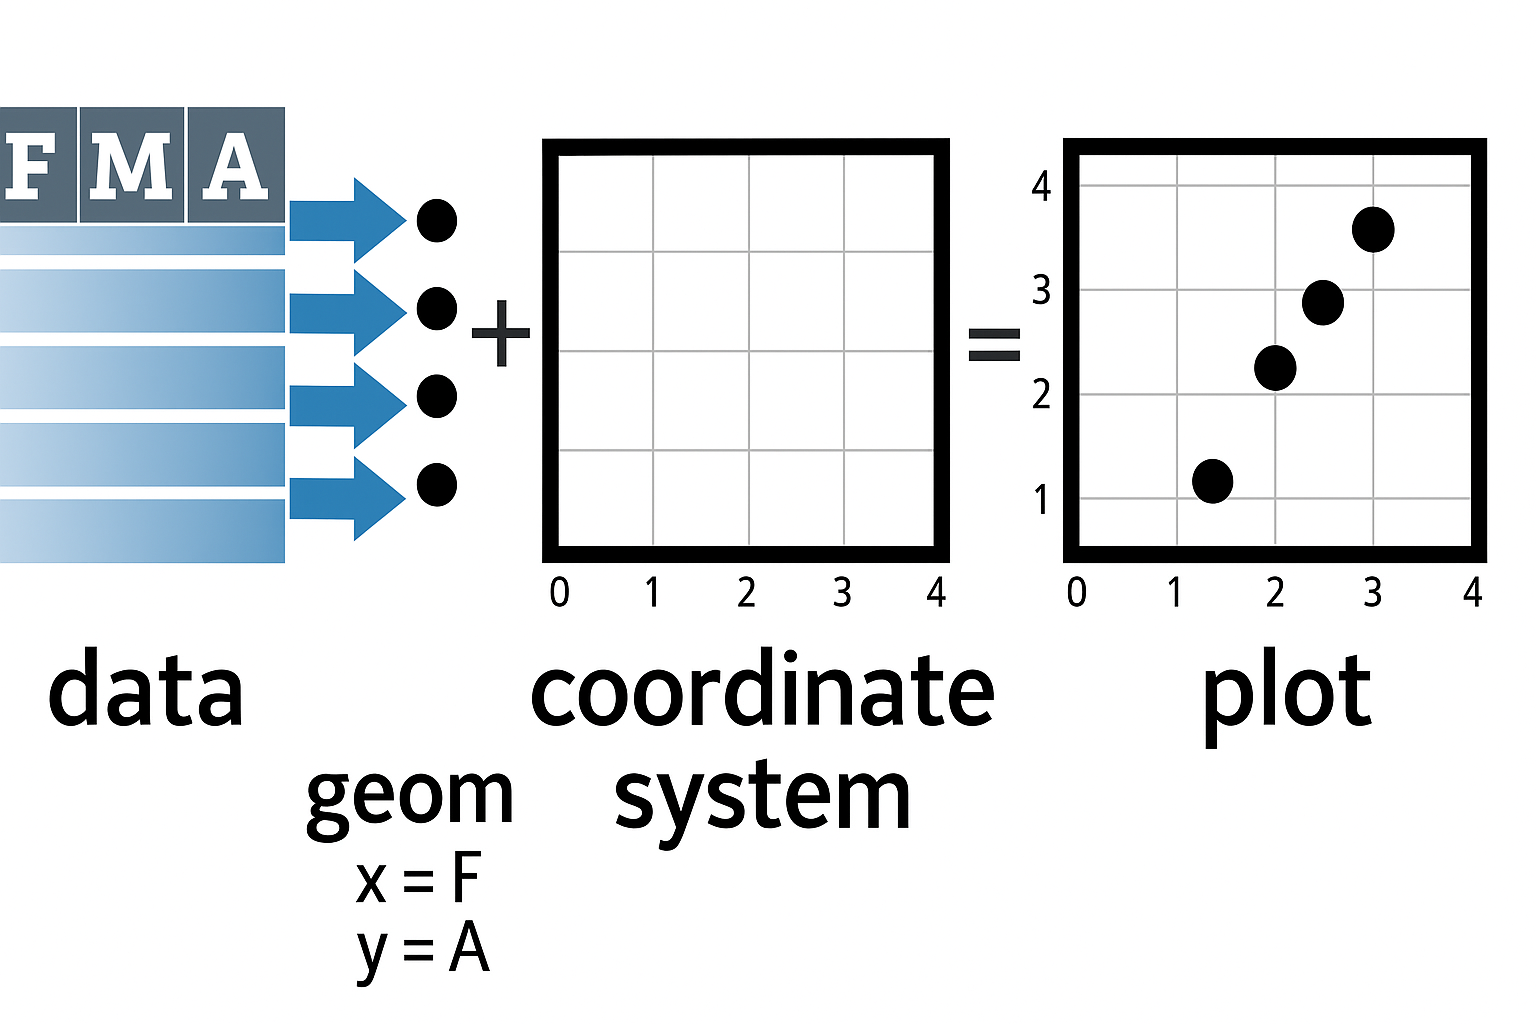
\includegraphics[width=0.5\linewidth,height=\textheight,keepaspectratio]{unidad_1/images/ggplot_estruct.png}
\end{center}

\section{\texorpdfstring{Anatomía de gráficos con
\texttt{ggplot2}}{Anatomía de gráficos con ggplot2}}\label{anatomuxeda-de-gruxe1ficos-con-ggplot2}

La construcción de gráficos en \texttt{ggplot2} se organiza a partir de
una gramática que puede entenderse a través de sus componentes
fundamentales:

\protect\phantomsection\label{fig1}
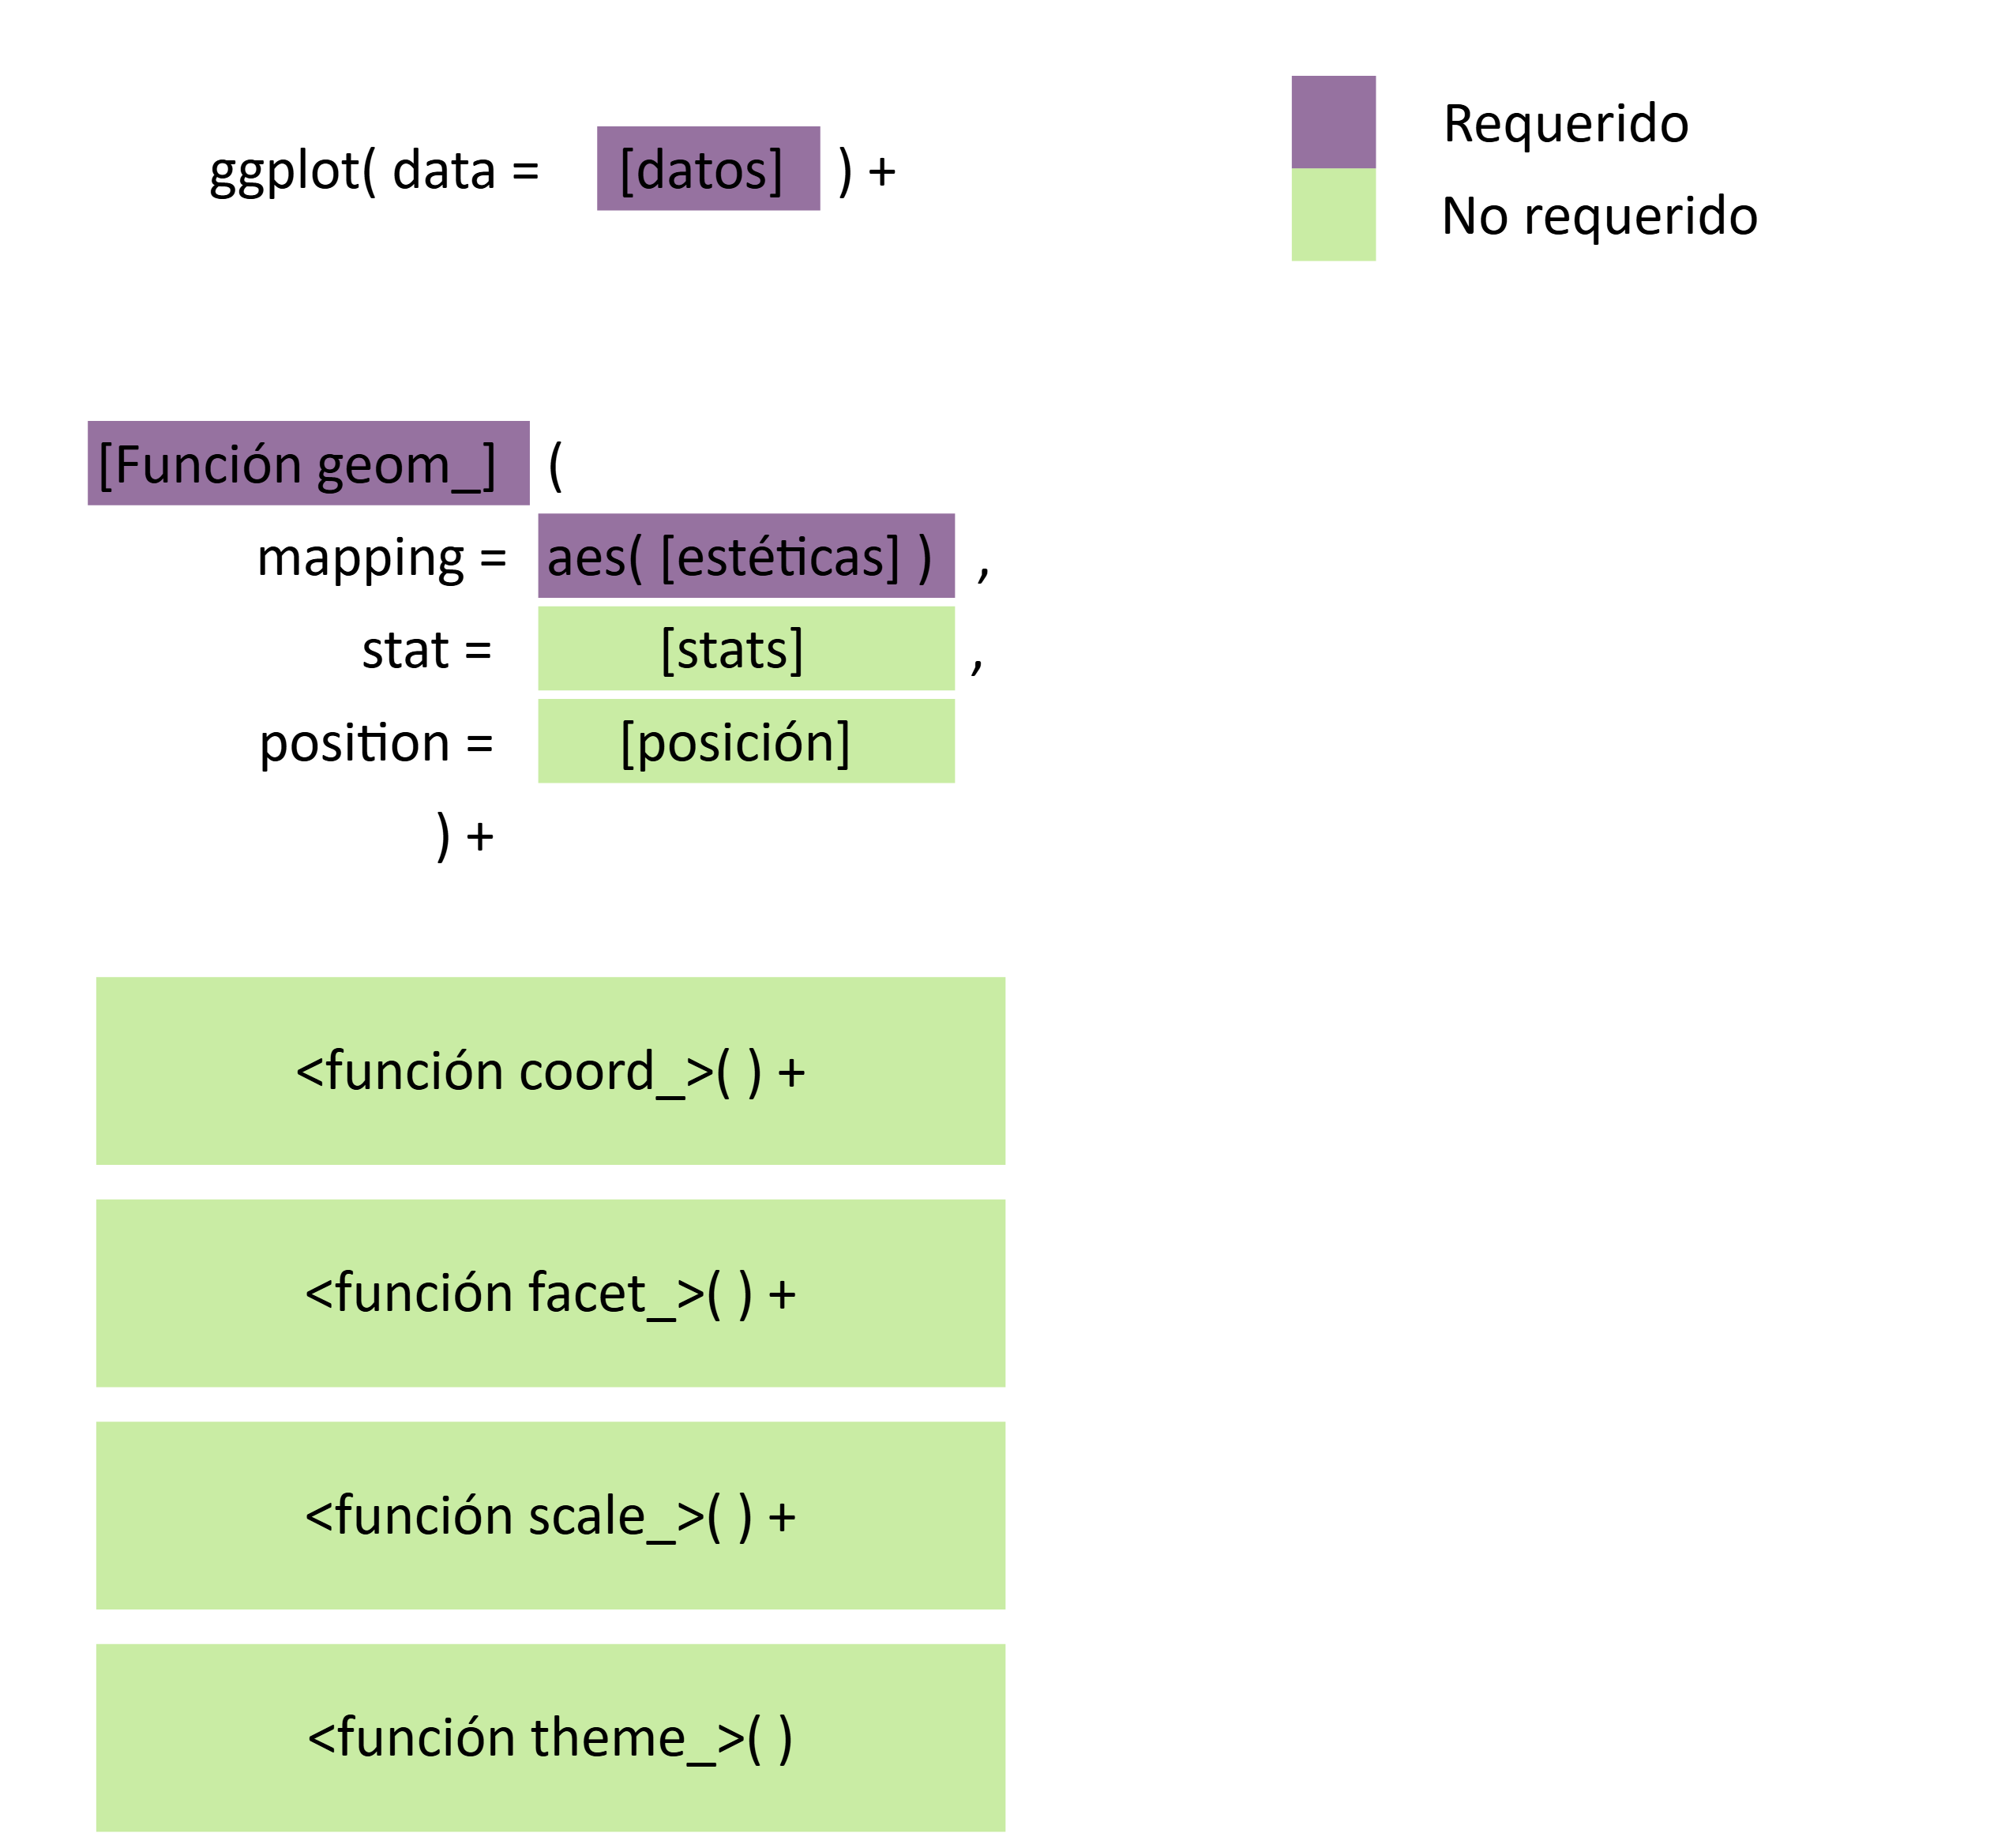
\includegraphics[width=5.5in,height=3.5in]{unidad_1/05_intro_ggplot_files/figure-latex/dot-figure-2.png}

\begin{itemize}
\tightlist
\item
  \texttt{data}: el conjunto de datos que vamos a graficar, debe
  contener toda la información necesaria.
\item
  \texttt{aes()}: el mapeo estético (\emph{aesthetic mapping}) es donde
  se declaran las variables que se representarán en el gráfico (por
  ejemplo, los ejes X e Y o cómo se asignarán los colores).
\item
  \texttt{geoms}: representaciones gráficas de los datos (puntos,
  líneas, barras, cajas, etc.). Son las ``geometrías'' que dibujan el
  gráfico.
\item
  \texttt{stats}: transformaciones estadísticas sobre los datos (medias,
  regresiones, suavizados, etc.), que permiten resumir la información.
\item
  \texttt{scales}: controlan cómo se representan los datos (ejes,
  colores, leyendas).
\item
  \texttt{coordinate\ systems}: sistema de coordenadas utilizado para
  representar el gráfico en un plano bidimensional.
\item
  \texttt{facets}:permiten dividir los datos en subconjuntos y generar
  gráficos en paneles (viñetas).
\item
  \texttt{theme}: controla la apariencia general de los elementos no
  asociados a los datos (fondos, tipografías, bordes, etc.).
\end{itemize}

\subsection{Ejemplo con datos}\label{ejemplo-con-datos}

Antes de mostrar como usar estos componentes, cargaremos la base de
datos ``\texttt{facultad.csv}'', que contiene datos ficticios sobre
ingresantes a una facultad (por ejemplo, sexo, edad, talla y peso). Este
conjunto se utilizará en los ejemplos:

\begin{Shaded}
\begin{Highlighting}[]
\CommentTok{\# Cargar datos}
\NormalTok{facultad }\OtherTok{\textless{}{-}} \FunctionTok{read\_csv}\NormalTok{(}\StringTok{"datos/facultad.csv"}\NormalTok{)}

\CommentTok{\# Mostramos las 6 primeras observaciones}
\FunctionTok{head}\NormalTok{(facultad)}
\end{Highlighting}
\end{Shaded}

\begin{verbatim}
# A tibble: 6 x 18
     hc sexo   edad ant_diabetes ant_tbc ant_cancer ant_obesidad ant_ecv ant_ht
  <dbl> <chr> <dbl> <chr>        <chr>   <chr>      <chr>        <chr>   <chr> 
1 26880 M        17 NO           NO      NO         SI           NO      SI    
2 26775 M        18 SI           NO      NO         NO           NO      NO    
3 26877 M        18 SI           NO      SI         NO           NO      SI    
4 26776 M        18 NO           NO      NO         SI           SI      NO    
5 26718 M        18 NO           NO      NO         NO           NO      SI    
6 26738 M        18 NO           NO      NO         NO           NO      SI    
# i 9 more variables: ant_col <chr>, fuma <chr>, edadini <dbl>, cantidad <dbl>,
#   col <dbl>, peso <dbl>, talla <dbl>, sist <dbl>, diast <dbl>
\end{verbatim}

\subsection{Mapeo estético}\label{mapeo-estuxe9tico}

La función básica para construir un gráfico en \texttt{ggplot2} es
\texttt{ggplot()}, que crea una estructura inicial (vacía) a la que le
irán agregando capas. Anteriormente dijimos que la función
\texttt{aes()} define el contenido estético del gráfico, es decir,
indica cómo se representan visualmente las variables (posición, color,
tamaño, forma, etc.).

Es importante notar que: - Si aes() se incluye dentro de ggplot(), el
mapeo se aplica a todas las capas. - Si se incluye dentro de una
geometría, se aplica solo a esa capa. - aes() genera automáticamente
leyendas cuando corresponde.

Veamos cómo funciona y cuáles son sus implicancias:

\begin{Shaded}
\begin{Highlighting}[]
\NormalTok{facultad }\SpecialCharTok{|\textgreater{}}
  \CommentTok{\# solo la capa estética aes()}
  \FunctionTok{ggplot}\NormalTok{(}\FunctionTok{aes}\NormalTok{(}\AttributeTok{x =}\NormalTok{ talla, }\AttributeTok{y =}\NormalTok{ peso))}
\end{Highlighting}
\end{Shaded}

\begin{center}
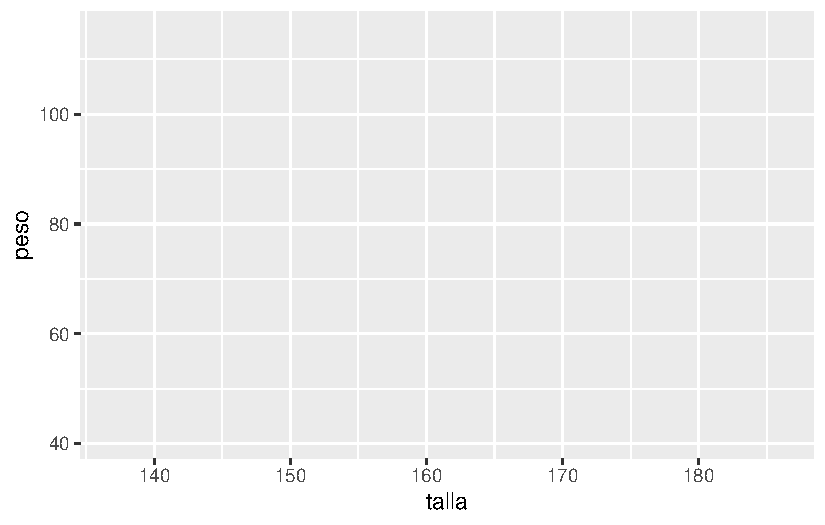
\includegraphics[width=0.85\linewidth,height=\textheight,keepaspectratio]{unidad_1/05_intro_ggplot_files/figure-pdf/cod2-1.pdf}
\end{center}

Este código genera un gráfico vacío que contiene únicamente los ejes
definidos (\texttt{peso} y \texttt{talla}), pero aún no muestra los
datos.

\subsection{Capas geométricas}\label{capas-geomuxe9tricas}

Para visualizar los datos, es necesario agregar capas geométricas
mediante funciones \texttt{geom\_}. Estas representan los objetos
gráficos que se dibujan en el gráfico.

Las capas se agregan utilizando el operador \texttt{+}:

\begin{Shaded}
\begin{Highlighting}[]
\NormalTok{facultad }\SpecialCharTok{|\textgreater{}}
  \CommentTok{\# mapeo estético}
  \FunctionTok{ggplot}\NormalTok{(}\FunctionTok{aes}\NormalTok{(}\AttributeTok{x =}\NormalTok{ talla, }\AttributeTok{y =}\NormalTok{ peso)) }\SpecialCharTok{+}

  \CommentTok{\# agregamos la capa geométrica de puntos}
  \FunctionTok{geom\_point}\NormalTok{()}
\end{Highlighting}
\end{Shaded}

\begin{center}
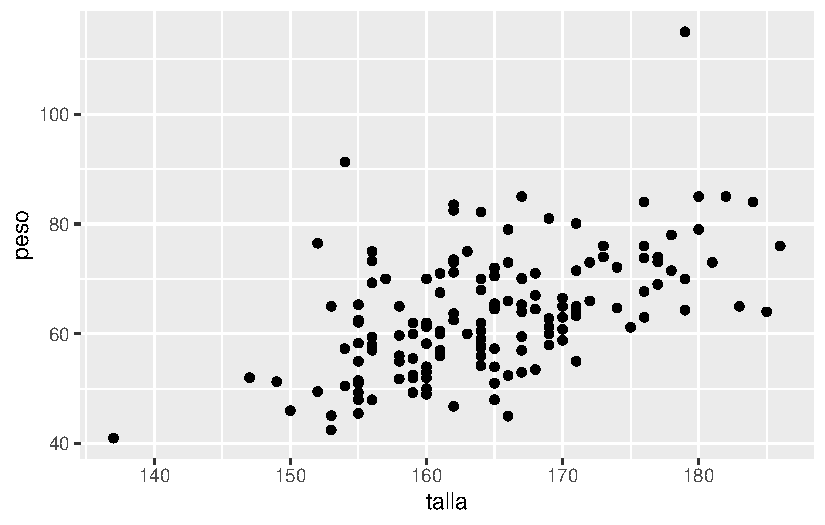
\includegraphics[width=0.85\linewidth,height=\textheight,keepaspectratio]{unidad_1/05_intro_ggplot_files/figure-pdf/cod3-1.pdf}
\end{center}

Podemos diferenciar los puntos según \texttt{sexo} incorporando esa
variable al mapeo estético:

\begin{Shaded}
\begin{Highlighting}[]
\NormalTok{facultad }\SpecialCharTok{|\textgreater{}}
  \CommentTok{\# mapeo estético}
  \FunctionTok{ggplot}\NormalTok{(}\FunctionTok{aes}\NormalTok{(}\AttributeTok{x =}\NormalTok{ talla, }\AttributeTok{y =}\NormalTok{ peso, }\AttributeTok{color =}\NormalTok{ sexo)) }\SpecialCharTok{+}

  \CommentTok{\# agregamos la capa geométrica de puntos}
  \FunctionTok{geom\_point}\NormalTok{()}
\end{Highlighting}
\end{Shaded}

\begin{center}
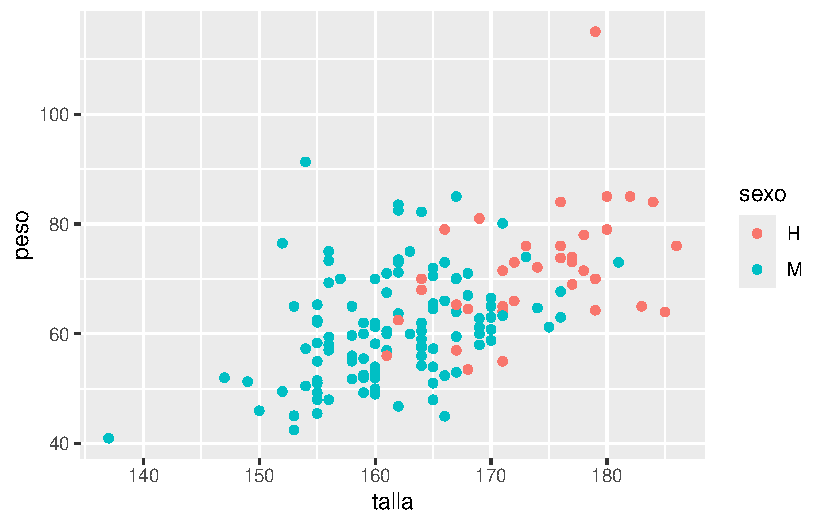
\includegraphics[width=0.85\linewidth,height=\textheight,keepaspectratio]{unidad_1/05_intro_ggplot_files/figure-pdf/cod4-1.pdf}
\end{center}

También es posible superponer capas. Por ejemplo, agregar rectas de
regresión:

\begin{Shaded}
\begin{Highlighting}[]
\NormalTok{facultad }\SpecialCharTok{|\textgreater{}}
  \CommentTok{\# mapeo estético}
  \FunctionTok{ggplot}\NormalTok{(}\FunctionTok{aes}\NormalTok{(}\AttributeTok{x =}\NormalTok{ talla, }\AttributeTok{y =}\NormalTok{ peso, }\AttributeTok{color =}\NormalTok{ sexo)) }\SpecialCharTok{+}

  \CommentTok{\# agregamos la capa geométrica de puntos}
  \FunctionTok{geom\_point}\NormalTok{() }\SpecialCharTok{+}

  \CommentTok{\# agregamos una segunda capa geométrica para la recta de regresión}
  \FunctionTok{geom\_smooth}\NormalTok{(}\AttributeTok{method =} \StringTok{"lm"}\NormalTok{)}
\end{Highlighting}
\end{Shaded}

\begin{center}
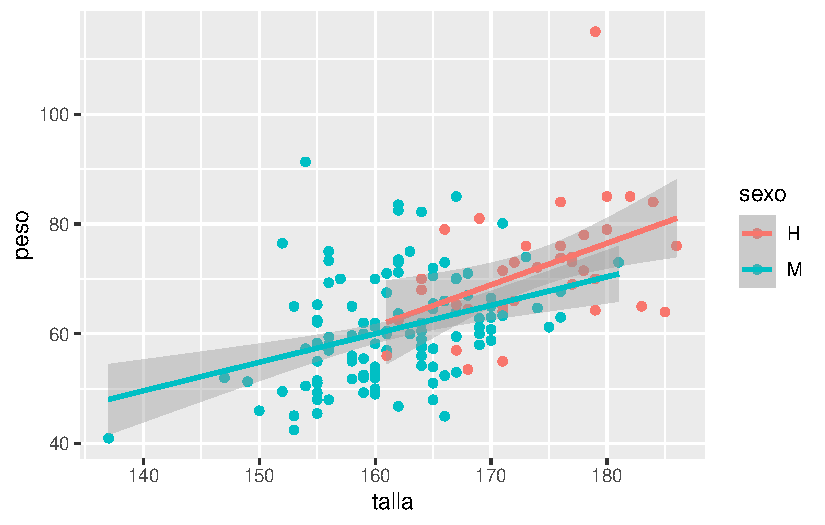
\includegraphics[width=0.85\linewidth,height=\textheight,keepaspectratio]{unidad_1/05_intro_ggplot_files/figure-pdf/cod5-1.pdf}
\end{center}

La función \texttt{geom\_smooth()} permite aplicar distintos métodos de
ajuste. En este caso, \texttt{"lm"} indica una regresión lineal,
incluyendo su intervalo de confianza.

Algunas de las capas geométricas más utilizadas son:

\begin{itemize}
\item
  Histogramas: \texttt{geom\_histogram()}
\item
  Gráfico de caja y bigotes (\emph{boxplot}): \texttt{geom\_boxplot()}
\item
  Gráfico de barras: \texttt{geom\_bar()}
\item
  Gráfico de columnas: \texttt{geom\_col()}
\item
  Gráfico de puntos (\emph{scatter plot}): \texttt{geom\_point()} o
  \texttt{geom\_jitter()}
\item
  Gráfico de líneas: \texttt{geom\_line()} o \texttt{geom\_path()}
\item
  Gráfico de violín: \texttt{geom\_violin()}
\item
  Tendencias: \texttt{geom\_smooth()}
\item
  Curvas de densidad: \texttt{geom\_density()}
\end{itemize}

Todas estas funciones pueden aplicarse sobre los mismos datos, y su uso
depende del objetivo del análisis. Las capas se grafican
secuencialmente, de modo que la última geometría en añadirse aparece
adelante.

A continuación, algunos ejemplos para visualizar la relación entre
\texttt{sexo} y \texttt{talla} utilizando distintas capas geométricas:

\begin{Shaded}
\begin{Highlighting}[]
\CommentTok{\# Gráfico de puntos}
\NormalTok{facultad }\SpecialCharTok{|\textgreater{}}
  \FunctionTok{ggplot}\NormalTok{(}\FunctionTok{aes}\NormalTok{(}\AttributeTok{x =}\NormalTok{ sexo, }\AttributeTok{y =}\NormalTok{ talla, }\AttributeTok{color =}\NormalTok{ sexo)) }\SpecialCharTok{+}
  \CommentTok{\# capa geométrica de puntos}
  \FunctionTok{geom\_point}\NormalTok{()}
\end{Highlighting}
\end{Shaded}

\begin{center}
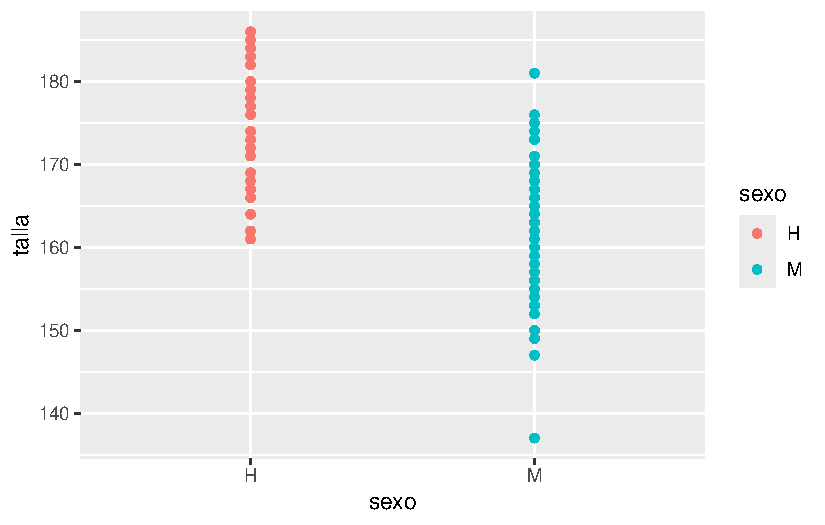
\includegraphics[width=0.85\linewidth,height=\textheight,keepaspectratio]{unidad_1/05_intro_ggplot_files/figure-pdf/cod6-1.pdf}
\end{center}

\begin{Shaded}
\begin{Highlighting}[]
\CommentTok{\# Boxplot}
\NormalTok{facultad }\SpecialCharTok{|\textgreater{}}
  \FunctionTok{ggplot}\NormalTok{(}\FunctionTok{aes}\NormalTok{(}\AttributeTok{x =}\NormalTok{ sexo, }\AttributeTok{y =}\NormalTok{ talla, }\AttributeTok{color =}\NormalTok{ sexo)) }\SpecialCharTok{+}
  \CommentTok{\# capa geométrica de boxplot}
  \FunctionTok{geom\_boxplot}\NormalTok{()}
\end{Highlighting}
\end{Shaded}

\begin{center}
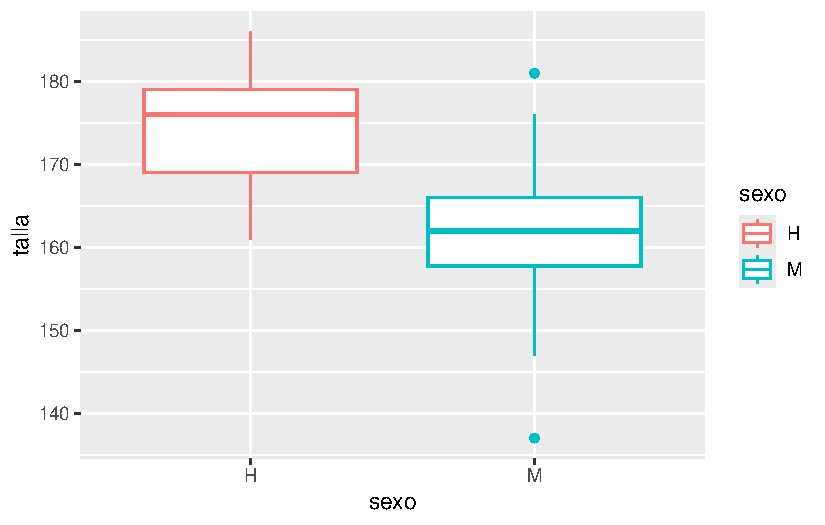
\includegraphics[width=0.85\linewidth,height=\textheight,keepaspectratio]{unidad_1/05_intro_ggplot_files/figure-pdf/cod6-2.pdf}
\end{center}

\begin{Shaded}
\begin{Highlighting}[]
\CommentTok{\# Entramado de puntos}
\NormalTok{facultad }\SpecialCharTok{|\textgreater{}}
  \FunctionTok{ggplot}\NormalTok{(}\FunctionTok{aes}\NormalTok{(}\AttributeTok{x =}\NormalTok{ sexo, }\AttributeTok{y =}\NormalTok{ talla, }\AttributeTok{color =}\NormalTok{ sexo)) }\SpecialCharTok{+}
  \CommentTok{\# capa geométrica jitter (entramado de puntos)}
  \FunctionTok{geom\_jitter}\NormalTok{()}
\end{Highlighting}
\end{Shaded}

\begin{center}
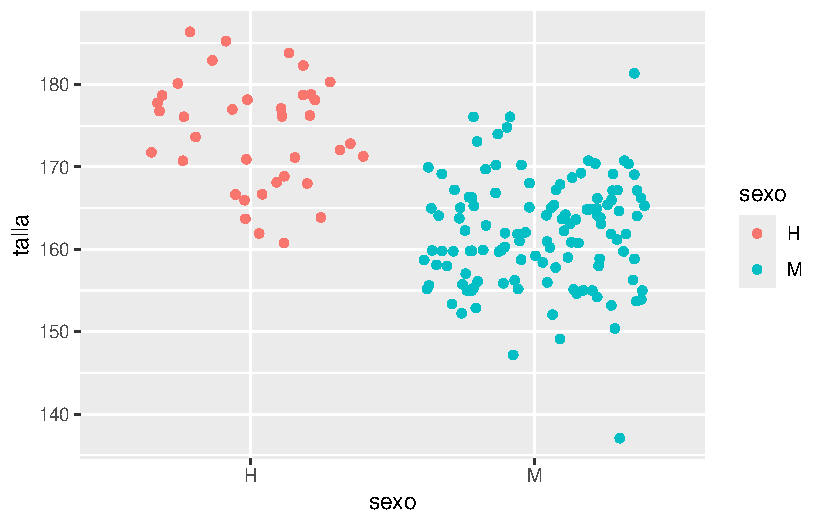
\includegraphics[width=0.85\linewidth,height=\textheight,keepaspectratio]{unidad_1/05_intro_ggplot_files/figure-pdf/cod6-3.pdf}
\end{center}

\begin{Shaded}
\begin{Highlighting}[]
\CommentTok{\# Gráfico de violín}
\NormalTok{facultad }\SpecialCharTok{|\textgreater{}}
  \FunctionTok{ggplot}\NormalTok{(}\FunctionTok{aes}\NormalTok{(}\AttributeTok{x =}\NormalTok{ sexo, }\AttributeTok{y =}\NormalTok{ talla, }\AttributeTok{fill =}\NormalTok{ sexo)) }\SpecialCharTok{+}
  \CommentTok{\# capa geométrica de violin}
  \FunctionTok{geom\_violin}\NormalTok{()}
\end{Highlighting}
\end{Shaded}

\begin{center}
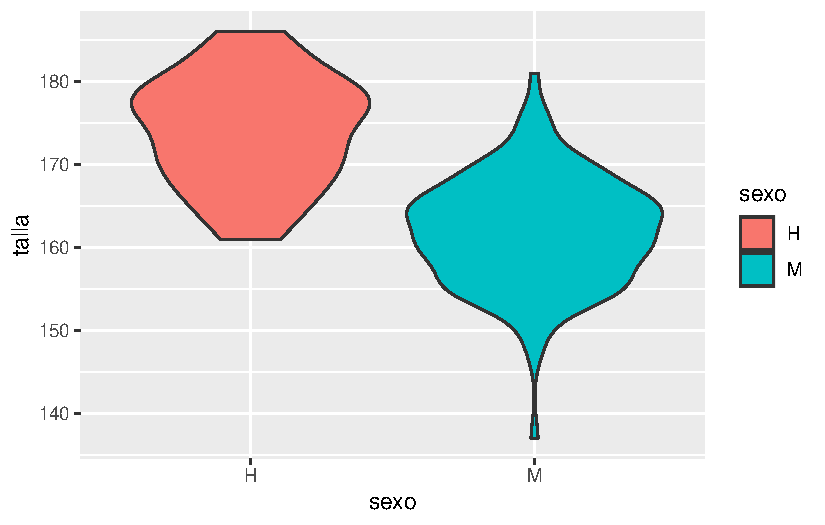
\includegraphics[width=0.85\linewidth,height=\textheight,keepaspectratio]{unidad_1/05_intro_ggplot_files/figure-pdf/cod6-4.pdf}
\end{center}

En el último caso se utiliza \texttt{fill} en lugar de \texttt{color}.
Mientras \texttt{color} controla el contorno, \texttt{fill} define el
relleno de las geometrías.

\subsection{Estéticas estáticas y
dinámicas}\label{estuxe9ticas-estuxe1ticas-y-dinuxe1micas}

En \texttt{ggplot2}, las estéticas son propiedades visuales asociadas a
los datos en las capas geométricas. No incluyen elementos como títulos o
etiquetas.

Algunas estéticas frecuentes:

\begin{itemize}
\item
  \texttt{color} / \texttt{colour}
\item
  \texttt{fill}
\item
  \texttt{alpha}
\item
  \texttt{size}
\item
  \texttt{linewidth} / \texttt{lwd}
\item
  \texttt{linetype}/ \texttt{lty}
\end{itemize}

\subsubsection{Valores estáticos}\label{valores-estuxe1ticos}

Si queremos que todas las observaciones tengan una misma estética,
colocamos los argumentos por fuera de \texttt{aes()}:

\begin{Shaded}
\begin{Highlighting}[]
\NormalTok{facultad }\SpecialCharTok{|\textgreater{}}
  \FunctionTok{ggplot}\NormalTok{(}\FunctionTok{aes}\NormalTok{(}\AttributeTok{x =}\NormalTok{ sexo, }\AttributeTok{y =}\NormalTok{ talla)) }\SpecialCharTok{+}
  \CommentTok{\# capa geométrica de puntos}
  \FunctionTok{geom\_point}\NormalTok{(}
    \AttributeTok{color =} \StringTok{"purple"}\NormalTok{, }\CommentTok{\# Color de los puntos}
    \AttributeTok{size =} \DecValTok{5}\NormalTok{, }\CommentTok{\# Tamaño de los puntos}
    \AttributeTok{alpha =}\NormalTok{ .}\DecValTok{5} \CommentTok{\# Transparencia de los puntos}
\NormalTok{  )}
\end{Highlighting}
\end{Shaded}

\begin{center}
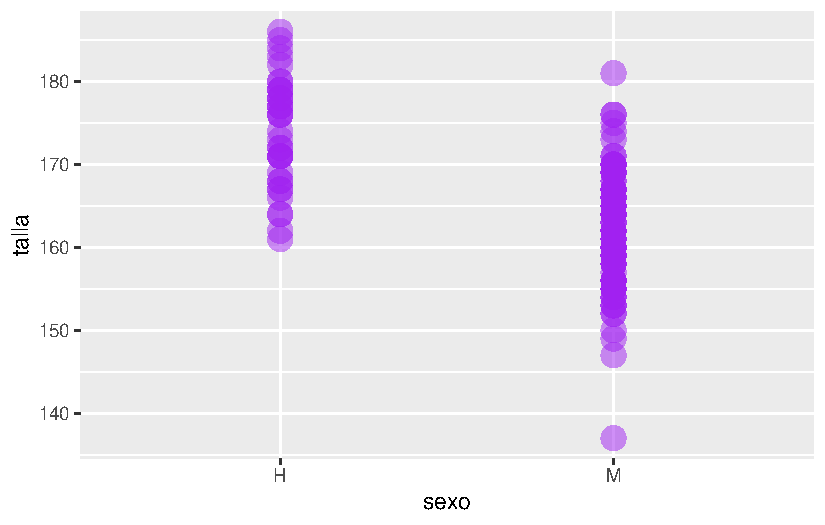
\includegraphics[width=0.85\linewidth,height=\textheight,keepaspectratio]{unidad_1/05_intro_ggplot_files/figure-pdf/cod7-1.pdf}
\end{center}

\subsubsection{Valores dinámicos}\label{valores-dinuxe1micos}

Se definen dentro de \texttt{aes()} y aplican a todas las capas:

\begin{Shaded}
\begin{Highlighting}[]
\NormalTok{facultad }\SpecialCharTok{|\textgreater{}}
  \CommentTok{\# Mapeo estético}
  \FunctionTok{ggplot}\NormalTok{(}\FunctionTok{aes}\NormalTok{(}\AttributeTok{x =}\NormalTok{ talla, }\AttributeTok{y =}\NormalTok{ peso, }\AttributeTok{color =}\NormalTok{ sexo)) }\SpecialCharTok{+}

  \CommentTok{\# agregamos la capa geométrica de puntos}
  \FunctionTok{geom\_point}\NormalTok{() }\SpecialCharTok{+}

  \CommentTok{\# agregamos una segunda capa geométrica para la recta de regresión}
  \FunctionTok{geom\_smooth}\NormalTok{(}\AttributeTok{method =} \StringTok{"lm"}\NormalTok{)}
\end{Highlighting}
\end{Shaded}

\begin{center}
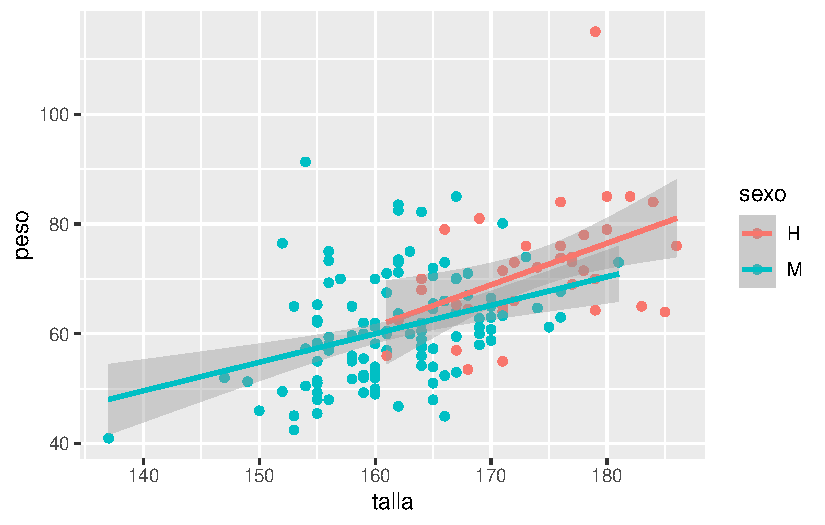
\includegraphics[width=0.85\linewidth,height=\textheight,keepaspectratio]{unidad_1/05_intro_ggplot_files/figure-pdf/cod8-1.pdf}
\end{center}

En este otro ejemplo, el color por sexo solo se aplica a los puntos de
\texttt{geom\_point()}, mientras que la regresión se calcula sobre el
conjunto completo:

\begin{Shaded}
\begin{Highlighting}[]
\NormalTok{facultad }\SpecialCharTok{|\textgreater{}}
  \CommentTok{\# mapeo estético}
  \FunctionTok{ggplot}\NormalTok{(}\FunctionTok{aes}\NormalTok{(}\AttributeTok{x =}\NormalTok{ talla, }\AttributeTok{y =}\NormalTok{ peso)) }\SpecialCharTok{+}

  \CommentTok{\# agregamos la capa geométrica de puntos coloreada por sexo}
  \FunctionTok{geom\_point}\NormalTok{(}\FunctionTok{aes}\NormalTok{(}\AttributeTok{color =}\NormalTok{ sexo)) }\SpecialCharTok{+}

  \CommentTok{\# agregamos una segunda capa geométrica para la recta de regresión}
  \FunctionTok{geom\_smooth}\NormalTok{(}\AttributeTok{method =} \StringTok{"lm"}\NormalTok{)}
\end{Highlighting}
\end{Shaded}

\begin{center}
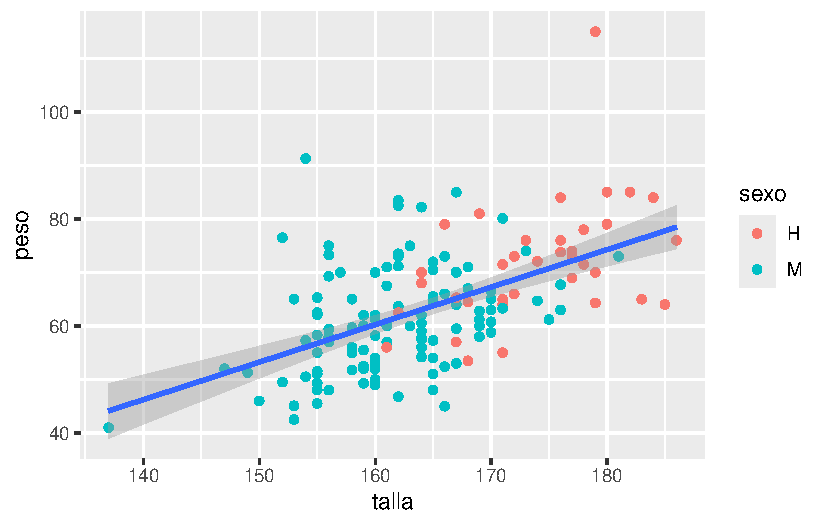
\includegraphics[width=0.85\linewidth,height=\textheight,keepaspectratio]{unidad_1/05_intro_ggplot_files/figure-pdf/cod9-1.pdf}
\end{center}

Este comportamiento permite una gran flexibilidad al construir gráficos,
definiendo qué capas responden a cada mapeo estético.

\section{Personalización de
escalas}\label{personalizaciuxf3n-de-escalas}

El sistema de escalas en \texttt{ggplot2} permite ajustar distintos
aspectos visuales de un gráfico, como colores de contorno y relleno,
ejes, tamaños y tipos de línea, entre otros.

Todas las funciones asociadas a escalas comienzan con el prefijo
\texttt{scale\_}, seguido del atributo que se desea modificar (por
ejemplo, \texttt{scale\_fill\_} para el color de relleno).

\subsection{Escalas de colores}\label{escalas-de-colores}

A continuación, se presentan algunos ejemplos utilizando el conjunto de
datos \texttt{facultad}:

\begin{Shaded}
\begin{Highlighting}[]
\NormalTok{facultad }\SpecialCharTok{|\textgreater{}}
  \FunctionTok{ggplot}\NormalTok{(}\FunctionTok{aes}\NormalTok{(}\AttributeTok{x =}\NormalTok{ sexo, }\AttributeTok{y =}\NormalTok{ talla, }\AttributeTok{fill =}\NormalTok{ sexo)) }\SpecialCharTok{+}

  \CommentTok{\# capa geométrica boxplot}
  \FunctionTok{geom\_boxplot}\NormalTok{() }\SpecialCharTok{+}

  \CommentTok{\# paleta de naranjas}
  \FunctionTok{scale\_fill\_brewer}\NormalTok{(}\AttributeTok{palette =} \StringTok{"Oranges"}\NormalTok{)}
\end{Highlighting}
\end{Shaded}

\begin{center}
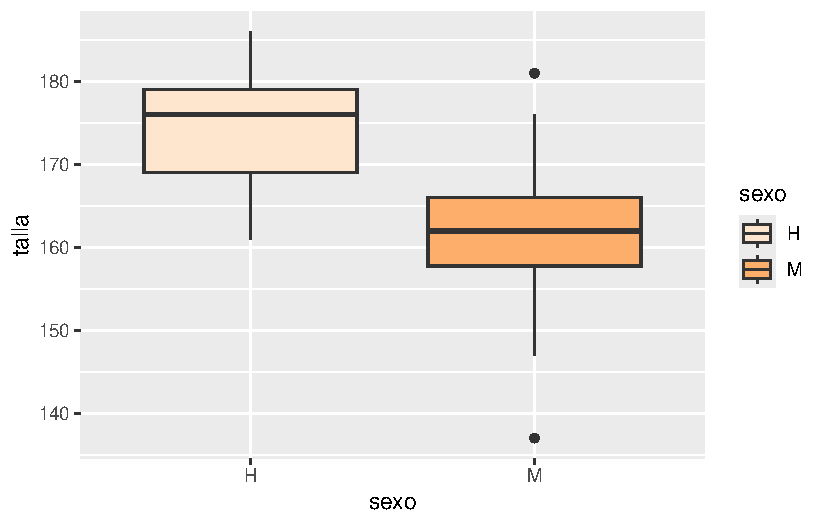
\includegraphics[width=0.85\linewidth,height=\textheight,keepaspectratio]{unidad_1/05_intro_ggplot_files/figure-pdf/cod10-1.pdf}
\end{center}

En este ejemplo, se aplica la función \texttt{scale\_fill\_brewer()},
que utiliza una paleta de colores (en este caso, \texttt{"Oranges"}) y
se vincula con el argumento \texttt{fill} definido en \texttt{aes()},
determinando el color de relleno del \emph{boxplot}.

Otra alternativa es utilizar una escala de grises mediante
\texttt{scale\_fill\_grey()}:

\begin{Shaded}
\begin{Highlighting}[]
\NormalTok{facultad }\SpecialCharTok{|\textgreater{}}
  \FunctionTok{ggplot}\NormalTok{(}\FunctionTok{aes}\NormalTok{(}\AttributeTok{x =}\NormalTok{ sexo, }\AttributeTok{y =}\NormalTok{ talla, }\AttributeTok{fill =}\NormalTok{ sexo)) }\SpecialCharTok{+}

  \CommentTok{\# capa geométrica boxplot}
  \FunctionTok{geom\_boxplot}\NormalTok{() }\SpecialCharTok{+}

  \CommentTok{\# paleta en escala de grises}
  \FunctionTok{scale\_fill\_grey}\NormalTok{(}\AttributeTok{start =} \FloatTok{0.4}\NormalTok{, }\AttributeTok{end =} \FloatTok{0.8}\NormalTok{)}
\end{Highlighting}
\end{Shaded}

\begin{center}
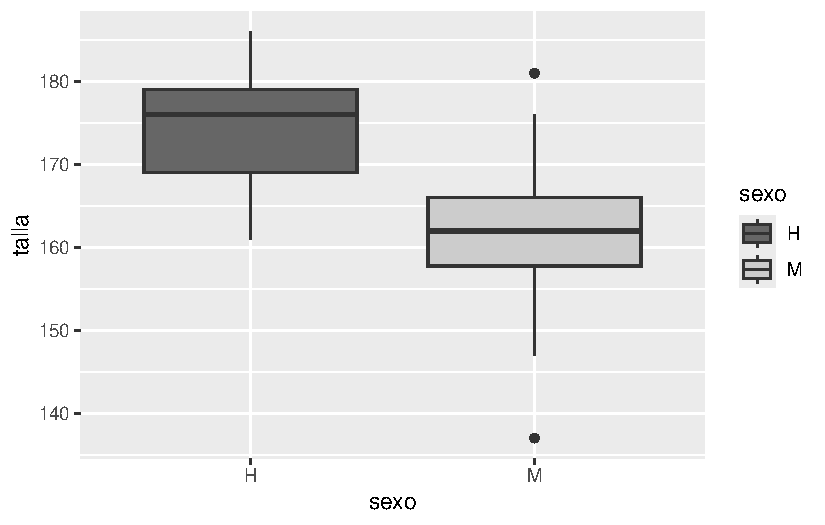
\includegraphics[width=0.85\linewidth,height=\textheight,keepaspectratio]{unidad_1/05_intro_ggplot_files/figure-pdf/cod11-1.pdf}
\end{center}

\begin{quote}
Se recomienda trabajar con paletas de colores accesibles para personas
con daltonismo y otras dificultades en la percepción visual, como las
incluidas en las dependencias \texttt{RColorBrewer} y
\texttt{viridisLite}, así como en paquetes específicos con paletas
\emph{colorblind-friendly}, como \texttt{scico} (Pedersen y Crameri
2023) y \texttt{cols4all} (Tennekes y Puts 2023).
\end{quote}

En versiones recientes de \texttt{ggplot2}, varias funciones de escala
permiten utilizar el argumento \texttt{aesthetics}, que facilita aplicar
una misma escala a múltiples estéticas simultáneamente. Esto resulta
especialmente útil cuando queremos usar una misma paleta de colores
tanto para el contorno (\texttt{color}) como para el relleno
(\texttt{fill}).

Retomando el ejemplo anterior:

\begin{Shaded}
\begin{Highlighting}[]
\NormalTok{facultad }\SpecialCharTok{|\textgreater{}}
  \FunctionTok{ggplot}\NormalTok{(}\FunctionTok{aes}\NormalTok{(}\AttributeTok{x =}\NormalTok{ sexo, }\AttributeTok{y =}\NormalTok{ talla, }\AttributeTok{fill =}\NormalTok{ sexo, }\AttributeTok{color =}\NormalTok{ sexo)) }\SpecialCharTok{+}

  \CommentTok{\# capa geométrica boxplot}
  \FunctionTok{geom\_boxplot}\NormalTok{() }\SpecialCharTok{+}

  \CommentTok{\# paleta en escala viridis}
  \FunctionTok{scale\_fill\_viridis\_d}\NormalTok{(}
    \AttributeTok{name =} \StringTok{"Género"}\NormalTok{,}
    \AttributeTok{aesthetics =} \FunctionTok{c}\NormalTok{(}\StringTok{"fill"}\NormalTok{, }\StringTok{"color"}\NormalTok{)}
\NormalTok{  )}
\end{Highlighting}
\end{Shaded}

\begin{center}
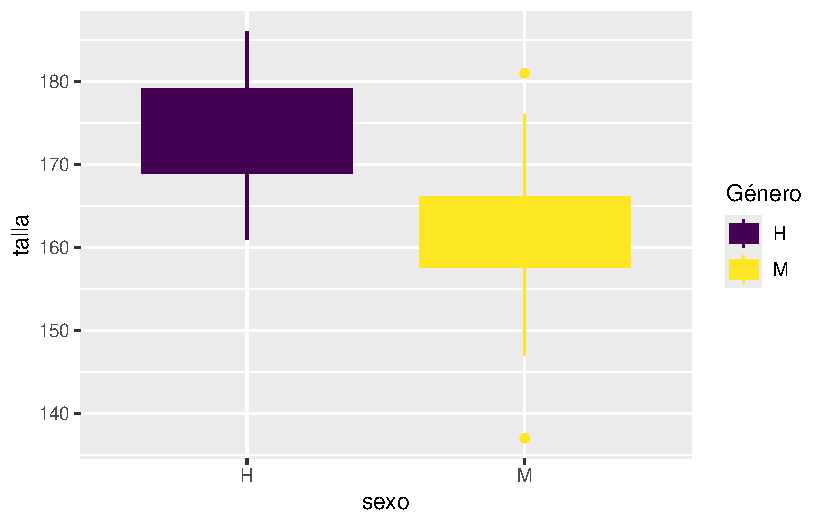
\includegraphics[width=0.85\linewidth,height=\textheight,keepaspectratio]{unidad_1/05_intro_ggplot_files/figure-pdf/cod12-1.pdf}
\end{center}

En este caso, la paleta \texttt{"viridis"} se aplica simultáneamente al
relleno y al contorno de las cajas, evitando inconsistencias visuales
entre ambas estéticas.

Sin \texttt{aesthetics} los colores de relleno y de línea deberían
especificarse como:

\begin{Shaded}
\begin{Highlighting}[]
\CommentTok{\# paleta en escala viridis}
\FunctionTok{scale\_fill\_viridis\_d}\NormalTok{(}\AttributeTok{name =} \StringTok{"Género"}\NormalTok{) }\SpecialCharTok{+}
  \FunctionTok{scale\_color\_viridis\_d}\NormalTok{()}
\end{Highlighting}
\end{Shaded}

Lo que duplica código y puede desincronizar los cambios en una paleta.

\subsection{Escalas de ejes}\label{escalas-de-ejes}

También es posible modificar las escalas de los ejes. Por ejemplo,
invertir el eje X con \texttt{scale\_x\_reverse()}:

\begin{Shaded}
\begin{Highlighting}[]
\NormalTok{facultad }\SpecialCharTok{|\textgreater{}}
  \FunctionTok{ggplot}\NormalTok{(}\FunctionTok{aes}\NormalTok{(}\AttributeTok{x =}\NormalTok{ talla, }\AttributeTok{y =}\NormalTok{ peso, }\AttributeTok{fill =}\NormalTok{ sexo)) }\SpecialCharTok{+}

  \CommentTok{\# capa geométrica de puntos}
  \FunctionTok{geom\_point}\NormalTok{() }\SpecialCharTok{+}

  \CommentTok{\# invierte el eje x}
  \FunctionTok{scale\_x\_reverse}\NormalTok{()}
\end{Highlighting}
\end{Shaded}

\begin{center}
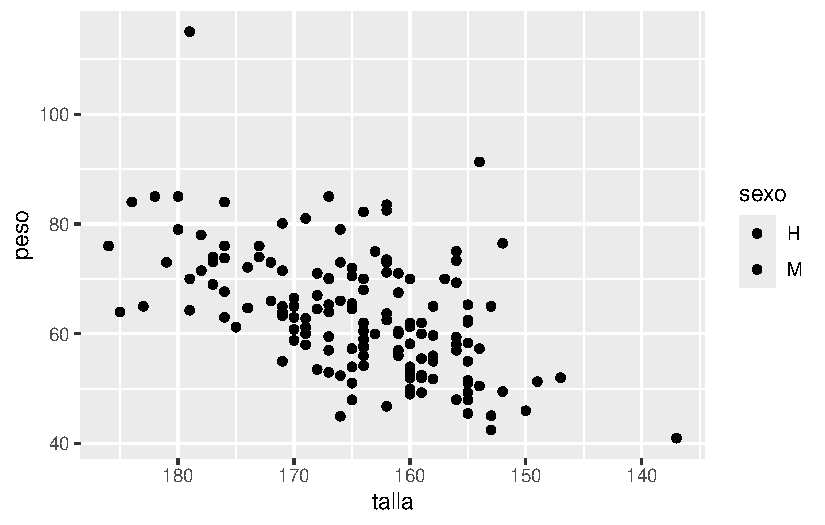
\includegraphics[width=0.85\linewidth,height=\textheight,keepaspectratio]{unidad_1/05_intro_ggplot_files/figure-pdf/cod14-1.pdf}
\end{center}

La inclusión de \texttt{scale\_x\_reverse()} provoca que la variable
\texttt{talla} se muestre en orden descendente (de mayor a menor).

Por último, se pueden personalizar los cortes del eje Y mediante
\texttt{scale\_y\_continuous()}. En el siguiente ejemplo, se define que
el eje Y vaya de 130 a 200 cm, con marcas cada 10 unidades:

\begin{Shaded}
\begin{Highlighting}[]
\NormalTok{facultad }\SpecialCharTok{|\textgreater{}}
  \FunctionTok{ggplot}\NormalTok{(}\FunctionTok{aes}\NormalTok{(}\AttributeTok{x =}\NormalTok{ sexo, }\AttributeTok{y =}\NormalTok{ talla, }\AttributeTok{fill =}\NormalTok{ sexo)) }\SpecialCharTok{+}

  \CommentTok{\# capa geométrica boxplot}
  \FunctionTok{geom\_boxplot}\NormalTok{() }\SpecialCharTok{+}

  \CommentTok{\# paleta en escala de grises}
  \FunctionTok{scale\_fill\_grey}\NormalTok{(}\AttributeTok{start =} \FloatTok{0.4}\NormalTok{, }\AttributeTok{end =} \FloatTok{0.8}\NormalTok{) }\SpecialCharTok{+}

  \CommentTok{\# puntos de corte del eje Y}
  \FunctionTok{scale\_y\_continuous}\NormalTok{(}
    \AttributeTok{limits =} \FunctionTok{c}\NormalTok{(}\DecValTok{130}\NormalTok{, }\DecValTok{200}\NormalTok{), }\CommentTok{\# límites}
    \AttributeTok{breaks =} \FunctionTok{seq}\NormalTok{(}\DecValTok{130}\NormalTok{, }\DecValTok{200}\NormalTok{, }\DecValTok{10}\NormalTok{)}
\NormalTok{  ) }\CommentTok{\# nro de etiquetas}
\end{Highlighting}
\end{Shaded}

\begin{center}
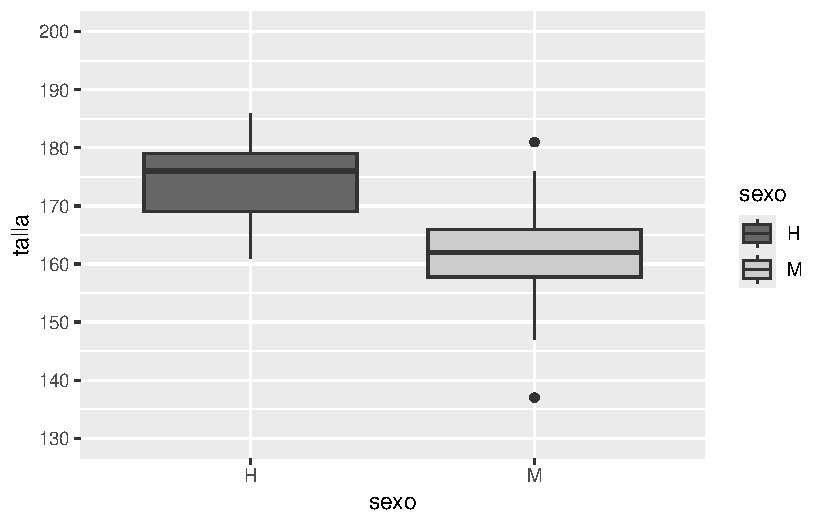
\includegraphics[width=0.85\linewidth,height=\textheight,keepaspectratio]{unidad_1/05_intro_ggplot_files/figure-pdf/cod15-1.pdf}
\end{center}

\section{Transformaciones
estadísticas}\label{transformaciones-estaduxedsticas}

En \texttt{ggplot2}, algunos gráficos no requieren transformaciones
estadísticas explícitas, como los gráficos de dispersión. Sin embargo,
otros ---como histogramas, \emph{boxplots} o curvas de tendencia---
incorporan \textbf{transformaciones estadísticas implícitas} que pueden
modificarse o personalizarse.

Estas transformaciones pueden:

\begin{itemize}
\item
  estar integradas dentro de las funciones geométricas (\texttt{geom\_})
\item
  agregarse como capas independientes mediante funciones \texttt{stat\_}
\end{itemize}

Por ejemplo, en un histograma la transformación estadística consiste en
agrupar los datos en intervalos (clases) y contar las observaciones en
cada uno. Esta transformación está incluida en
\texttt{geom\_histogram()}, pero puede parametrizarse:

\begin{Shaded}
\begin{Highlighting}[]
\NormalTok{facultad }\SpecialCharTok{|\textgreater{}}
  \FunctionTok{ggplot}\NormalTok{(}\FunctionTok{aes}\NormalTok{(edad)) }\SpecialCharTok{+}

  \CommentTok{\# capa geométrica histograma}
  \FunctionTok{geom\_histogram}\NormalTok{(}\AttributeTok{bins =} \FunctionTok{nclass.Sturges}\NormalTok{(facultad}\SpecialCharTok{$}\NormalTok{edad), }\AttributeTok{fill =} \StringTok{"Blue"}\NormalTok{)}
\end{Highlighting}
\end{Shaded}

\begin{center}
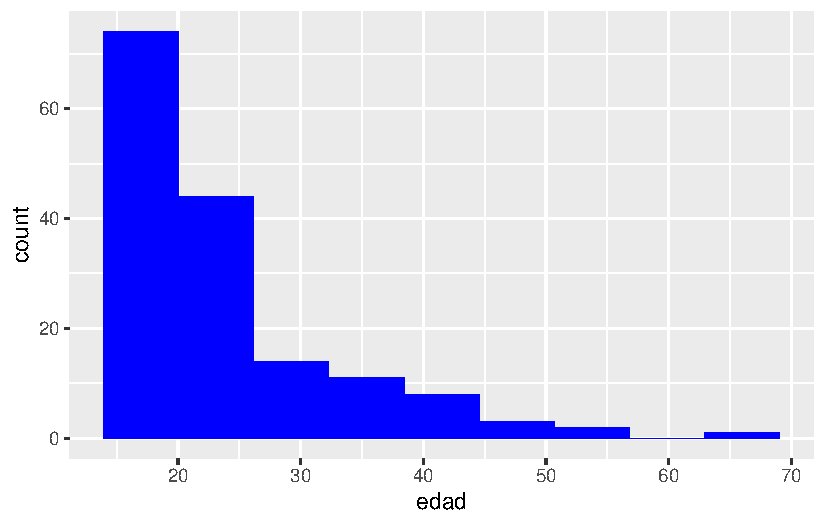
\includegraphics[width=0.85\linewidth,height=\textheight,keepaspectratio]{unidad_1/05_intro_ggplot_files/figure-pdf/cod16-1.pdf}
\end{center}

En este caso, se utiliza la regla de Sturges ---a través de
\texttt{nclass.Sturges()}--- para determinar automáticamente la cantidad
de clases de la variable \texttt{edad}.

También es posible agregar transformaciones estadísticas como capas
adicionales. Por ejemplo, si queremos mostrar la media de \texttt{talla}
para cada grupo de \texttt{sexo} sobre un \emph{boxplot}, podemos
utilizar \texttt{stat\_summary()}:

\begin{Shaded}
\begin{Highlighting}[]
\NormalTok{facultad }\SpecialCharTok{|\textgreater{}}
  \FunctionTok{ggplot}\NormalTok{(}\FunctionTok{aes}\NormalTok{(}\AttributeTok{x =}\NormalTok{ sexo, }\AttributeTok{y =}\NormalTok{ talla, }\AttributeTok{fill =}\NormalTok{ sexo)) }\SpecialCharTok{+}

  \CommentTok{\# capa geométrica boxplot}
  \FunctionTok{geom\_boxplot}\NormalTok{() }\SpecialCharTok{+}

  \CommentTok{\# paleta de tonos verdes}
  \FunctionTok{scale\_fill\_brewer}\NormalTok{(}\AttributeTok{palette =} \StringTok{"Greens"}\NormalTok{) }\SpecialCharTok{+}

  \CommentTok{\# añade capa summary}
  \FunctionTok{stat\_summary}\NormalTok{(}
    \AttributeTok{fun =}\NormalTok{ mean,}
    \AttributeTok{color =} \StringTok{"darkred"}\NormalTok{,}
    \AttributeTok{geom =} \StringTok{"point"}\NormalTok{,}
    \AttributeTok{shape =} \DecValTok{18}\NormalTok{,}
    \AttributeTok{size =} \DecValTok{3}
\NormalTok{  )}
\end{Highlighting}
\end{Shaded}

\begin{center}
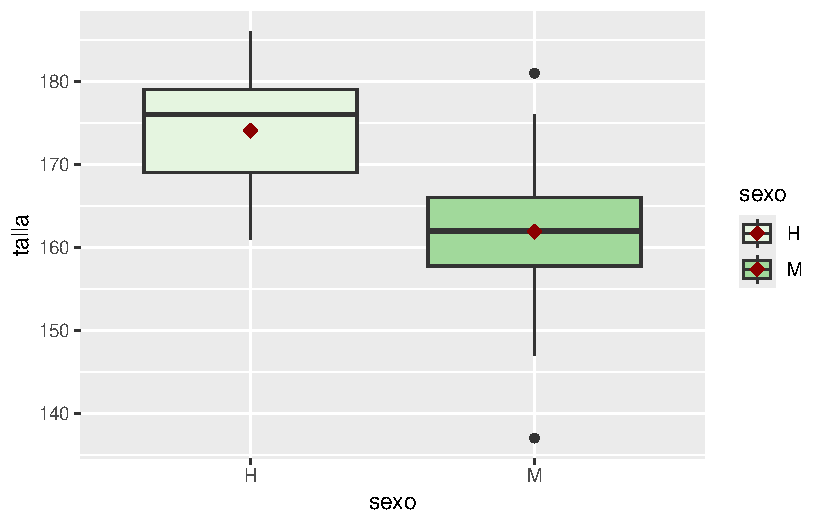
\includegraphics[width=0.85\linewidth,height=\textheight,keepaspectratio]{unidad_1/05_intro_ggplot_files/figure-pdf/cod17-1.pdf}
\end{center}

La función \texttt{stat\_summary()} permite calcular estadísticas (como
\texttt{mean}, \texttt{median}, \texttt{sd}, entre otras) y
representarlas mediante una geometría. En este caso, la media de
\texttt{talla} se muestra como un punto rojo oscuro
(\texttt{color\ =\ "darkred"}), con forma romboidal
(\texttt{shape\ =\ 18}) y tamaño destacado (\texttt{size\ =\ 3}).

\section{Facetado}\label{facetado}

El \textbf{facetado} permite dividir un gráfico en múltiples paneles (o
viñetas) según los niveles de una o más variables categóricas. Esto
resulta especialmente útil para comparar patrones entre grupos sin
sobrecargar un único gráfico.

En \texttt{ggplot2} existen dos funciones principales para implementar
esta técnica:

\begin{itemize}
\item
  \texttt{facet\_wrap()}: divide los datos según una única variable
  categórica, generando paneles dispuestos automáticamente en filas y
  columnas.
\item
  \texttt{facet\_grid()}: permite crear una matriz de paneles a partir
  de dos variables categóricas, una definida en las filas y otra en las
  columnas.
\end{itemize}

Retomemos el gráfico de dispersión entre \texttt{talla} y \texttt{peso},
y generemos paneles separados para cada nivel de la variable
\texttt{sexo} usando \texttt{facet\_wrap()}:

\begin{Shaded}
\begin{Highlighting}[]
\NormalTok{facultad }\SpecialCharTok{|\textgreater{}}

  \FunctionTok{ggplot}\NormalTok{(}\FunctionTok{aes}\NormalTok{(}\AttributeTok{x =}\NormalTok{ talla, }\AttributeTok{y =}\NormalTok{ peso, }\AttributeTok{color =}\NormalTok{ sexo)) }\SpecialCharTok{+}

  \CommentTok{\# capa geométrica de puntos}
  \FunctionTok{geom\_point}\NormalTok{() }\SpecialCharTok{+}

  \CommentTok{\# separa en paneles por sexo}
  \FunctionTok{facet\_wrap}\NormalTok{(}\SpecialCharTok{\textasciitilde{}}\NormalTok{sexo)}
\end{Highlighting}
\end{Shaded}

\begin{center}
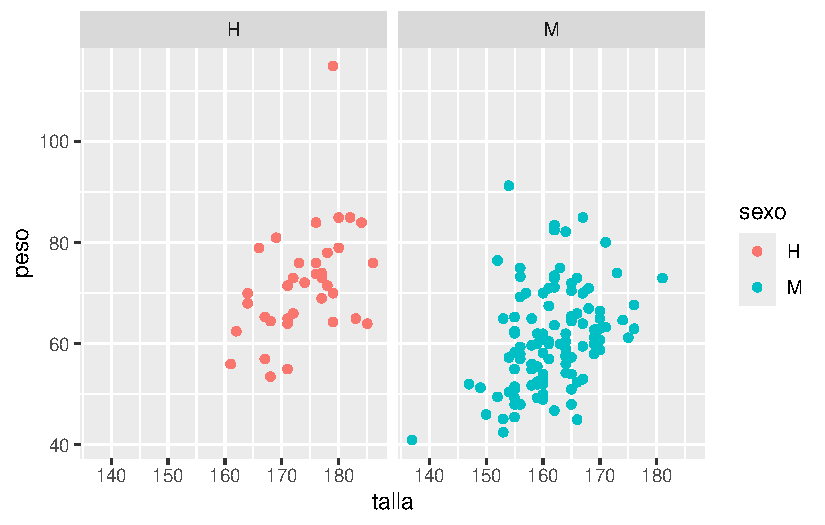
\includegraphics[width=0.85\linewidth,height=\textheight,keepaspectratio]{unidad_1/05_intro_ggplot_files/figure-pdf/cod18-1.pdf}
\end{center}

Ahora utilizamos \texttt{facet\_grid()} para crear una matriz de
histogramas a partir del cruce de las variables \texttt{sexo} y
\texttt{fuma}. En cada panel se representa la distribución de
\texttt{peso}:

\begin{Shaded}
\begin{Highlighting}[]
\NormalTok{facultad }\SpecialCharTok{|\textgreater{}}
  \FunctionTok{ggplot}\NormalTok{(}\FunctionTok{aes}\NormalTok{(}\AttributeTok{y =}\NormalTok{ peso, }\AttributeTok{fill =}\NormalTok{ sexo)) }\SpecialCharTok{+}

  \CommentTok{\# capa geométrica histograma}
  \FunctionTok{geom\_histogram}\NormalTok{(}\AttributeTok{bins =} \FunctionTok{nclass.Sturges}\NormalTok{(facultad}\SpecialCharTok{$}\NormalTok{peso)) }\SpecialCharTok{+}

  \CommentTok{\# paleta de colores}
  \FunctionTok{scale\_fill\_brewer}\NormalTok{(}\AttributeTok{palette =} \StringTok{"Set2"}\NormalTok{) }\SpecialCharTok{+}

  \CommentTok{\# separa en paneles por sexo y fuma}
  \FunctionTok{facet\_grid}\NormalTok{(sexo }\SpecialCharTok{\textasciitilde{}}\NormalTok{ fuma)}
\end{Highlighting}
\end{Shaded}

\begin{center}
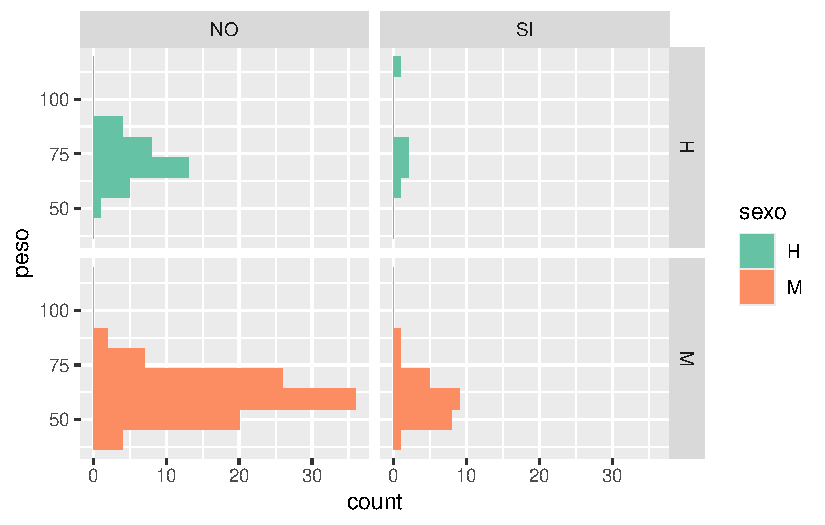
\includegraphics[width=0.85\linewidth,height=\textheight,keepaspectratio]{unidad_1/05_intro_ggplot_files/figure-pdf/cod19-1.pdf}
\end{center}

Como se observa en estos ejemplos, el facetado se integra naturalmente
con otros componentes de la gramática de gráficos: mapeo estético
(\texttt{aes()}), capas geométricas (\texttt{geom\_}) y escalas
(\texttt{scale\_}).

El número de combinaciones posibles es muy amplio, dada la flexibilidad
de \texttt{ggplot2}. Sin embargo, el objetivo de este material es
comprender los principios fundamentales sobre los que se construye esta
\emph{gramática de los gráficos}.

\section{Sistema de coordenadas}\label{sistema-de-coordenadas}

En algunos casos, puede ser útil modificar el sistema de coordenadas
predeterminado de un gráfico. Mientras que las funciones
\texttt{scale\_} controlan \textbf{cómo se representan los datos}, las
funciones de coordenadas (\texttt{coord\_}) modifican \textbf{cómo se
visualiza el espacio del gráfico}.

En \texttt{ggplot2} una de las transformaciones más comunes es invertir
la orientación de los ejes mediante \texttt{coord\_flip()}, lo que
resulta útil, por ejemplo, para presentar gráficos de barras en forma
horizontal:

\begin{Shaded}
\begin{Highlighting}[]
\NormalTok{facultad }\SpecialCharTok{|\textgreater{}}

  \FunctionTok{ggplot}\NormalTok{(}\FunctionTok{aes}\NormalTok{(sexo, }\AttributeTok{fill =}\NormalTok{ sexo)) }\SpecialCharTok{+}

  \CommentTok{\# capa geométrica barras}
  \FunctionTok{geom\_bar}\NormalTok{() }\SpecialCharTok{+}

  \CommentTok{\# paleta de colores}
  \FunctionTok{scale\_fill\_brewer}\NormalTok{(}\AttributeTok{palette =} \StringTok{"Set2"}\NormalTok{) }\SpecialCharTok{+}

  \CommentTok{\# invierte disposición de ejes}
  \FunctionTok{coord\_flip}\NormalTok{()}
\end{Highlighting}
\end{Shaded}

\begin{center}
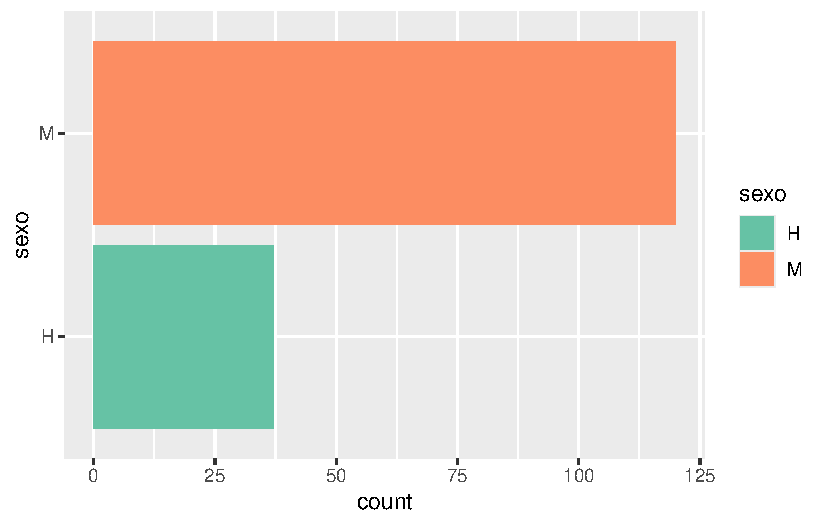
\includegraphics[width=0.85\linewidth,height=\textheight,keepaspectratio]{unidad_1/05_intro_ggplot_files/figure-pdf/cod20-1.pdf}
\end{center}

\section{Temas}\label{temas}

\texttt{ggplot2} incluye un conjunto de temas gráficos predefinidos que
permiten modificar el aspecto general del gráfico. El tema por defecto
es \texttt{theme\_gray()}, pero puede cambiarse agregando una capa
\texttt{theme\_*()} dentro del gráfico.

Repetimos el gráfico anterior, esta vez utilizando el tema blanco y
negro (\texttt{theme\_bw()}):

\begin{Shaded}
\begin{Highlighting}[]
\NormalTok{facultad }\SpecialCharTok{|\textgreater{}}

  \FunctionTok{ggplot}\NormalTok{(}\FunctionTok{aes}\NormalTok{(sexo, }\AttributeTok{fill =}\NormalTok{ sexo)) }\SpecialCharTok{+}

  \CommentTok{\# capa geométrica barras}
  \FunctionTok{geom\_bar}\NormalTok{() }\SpecialCharTok{+}

  \CommentTok{\# paleta de colores}
  \FunctionTok{scale\_fill\_brewer}\NormalTok{(}\AttributeTok{palette =} \StringTok{"Set2"}\NormalTok{) }\SpecialCharTok{+}

  \CommentTok{\# invierte disposición de ejes}
  \FunctionTok{coord\_flip}\NormalTok{() }\SpecialCharTok{+}

  \CommentTok{\# tema en blanco y negro}
  \FunctionTok{theme\_bw}\NormalTok{()}
\end{Highlighting}
\end{Shaded}

\begin{center}
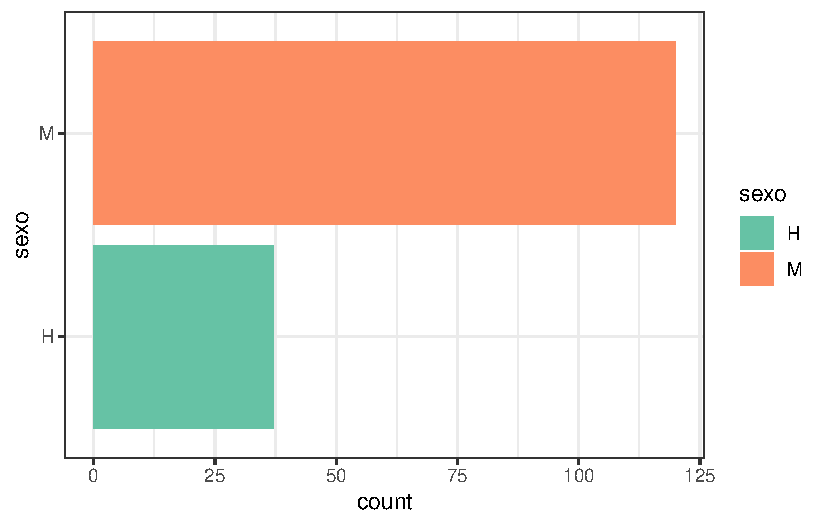
\includegraphics[width=0.85\linewidth,height=\textheight,keepaspectratio]{unidad_1/05_intro_ggplot_files/figure-pdf/cod21-1.pdf}
\end{center}

También podemos aplicar un tema de fondo oscuro con
\texttt{theme\_dark()}:

\begin{Shaded}
\begin{Highlighting}[]
\NormalTok{facultad }\SpecialCharTok{|\textgreater{}}

  \FunctionTok{ggplot}\NormalTok{(}\FunctionTok{aes}\NormalTok{(sexo, }\AttributeTok{fill =}\NormalTok{ sexo)) }\SpecialCharTok{+}

  \CommentTok{\# capa geométrica barras}
  \FunctionTok{geom\_bar}\NormalTok{() }\SpecialCharTok{+}

  \CommentTok{\# paleta de colores}
  \FunctionTok{scale\_fill\_brewer}\NormalTok{(}\AttributeTok{palette =} \StringTok{"Set2"}\NormalTok{) }\SpecialCharTok{+}

  \CommentTok{\# invierte disposición de ejes}
  \FunctionTok{coord\_flip}\NormalTok{() }\SpecialCharTok{+}

  \CommentTok{\# tema con fondo oscuro}
  \FunctionTok{theme\_dark}\NormalTok{()}
\end{Highlighting}
\end{Shaded}

\begin{center}
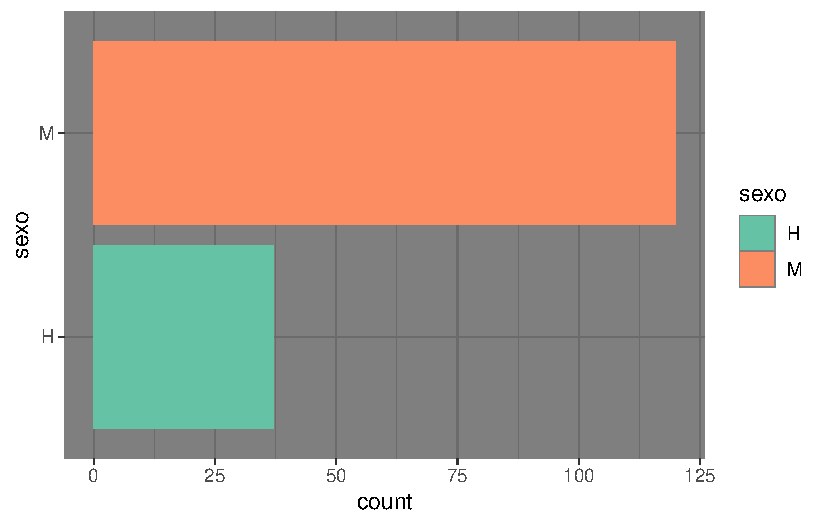
\includegraphics[width=0.85\linewidth,height=\textheight,keepaspectratio]{unidad_1/05_intro_ggplot_files/figure-pdf/cod22-1.pdf}
\end{center}

A continuación se muestra un cuadro con los principales temas
disponibles en \texttt{ggplot2} y sus características visuales:

\begin{center}
\pandocbounded{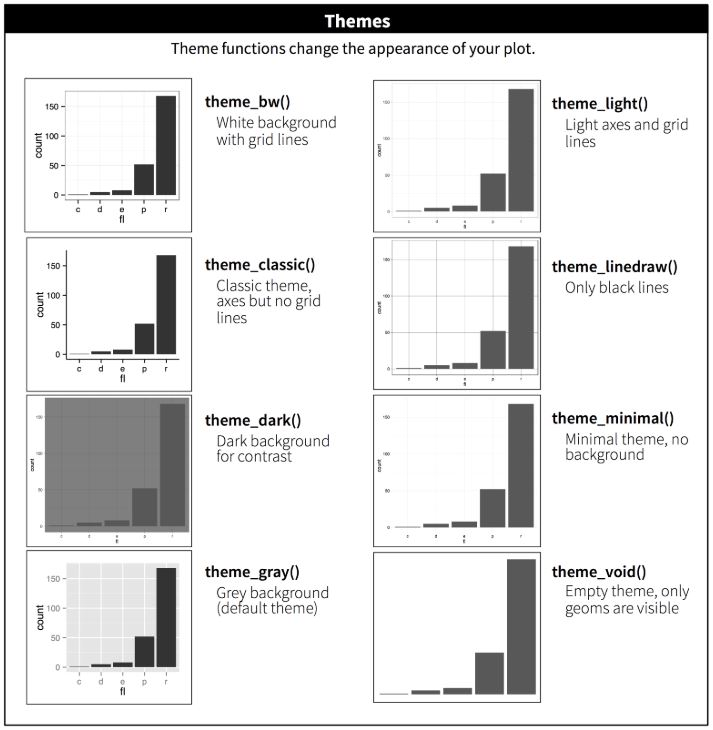
\includegraphics[keepaspectratio]{unidad_1/images/ggplot_temas.JPG}}
\end{center}

Además del aspecto general del gráfico, es posible agregar títulos,
subtítulos y etiquetas de ejes con la función \texttt{labs()}. Por
ejemplo:

\begin{Shaded}
\begin{Highlighting}[]
\FunctionTok{labs}\NormalTok{(}
  \AttributeTok{x =} \StringTok{"Etiqueta X"}\NormalTok{,}
  \AttributeTok{y =} \StringTok{"Etiqueta Y"}\NormalTok{,}
  \AttributeTok{title =} \StringTok{"Título del gráfico"}\NormalTok{,}
  \AttributeTok{subtitle =} \StringTok{"Subtítulo del gráfico"}
\NormalTok{)}
\end{Highlighting}
\end{Shaded}

También se pueden ajustar detalles del texto, como tipo de fuente o
tamaño, mediante la función \texttt{theme()}:

\begin{Shaded}
\begin{Highlighting}[]
\NormalTok{facultad }\SpecialCharTok{|\textgreater{}}
  \FunctionTok{ggplot}\NormalTok{(}\FunctionTok{aes}\NormalTok{(sexo, }\AttributeTok{fill =}\NormalTok{ sexo)) }\SpecialCharTok{+}
  \CommentTok{\# capa geométrica barras}
  \FunctionTok{geom\_bar}\NormalTok{() }\SpecialCharTok{+}
  \CommentTok{\# paleta de colores}
  \FunctionTok{scale\_fill\_brewer}\NormalTok{(}\AttributeTok{palette =} \StringTok{"Set2"}\NormalTok{) }\SpecialCharTok{+}
  \CommentTok{\# invierte disposición de ejes}
  \FunctionTok{coord\_flip}\NormalTok{() }\SpecialCharTok{+}
  \CommentTok{\# cambia etiquetas de los ejes}
  \FunctionTok{labs}\NormalTok{(}\AttributeTok{y =} \StringTok{"Cantidad"}\NormalTok{, }\AttributeTok{title =} \StringTok{"Distribución de sexo"}\NormalTok{) }\SpecialCharTok{+}
  \CommentTok{\# modifica el estilo de fuente del título}
  \FunctionTok{theme}\NormalTok{(}\AttributeTok{plot.title =} \FunctionTok{element\_text}\NormalTok{(}\AttributeTok{face =} \StringTok{"italic"}\NormalTok{, }\AttributeTok{size =} \DecValTok{16}\NormalTok{))}
\end{Highlighting}
\end{Shaded}

\begin{center}
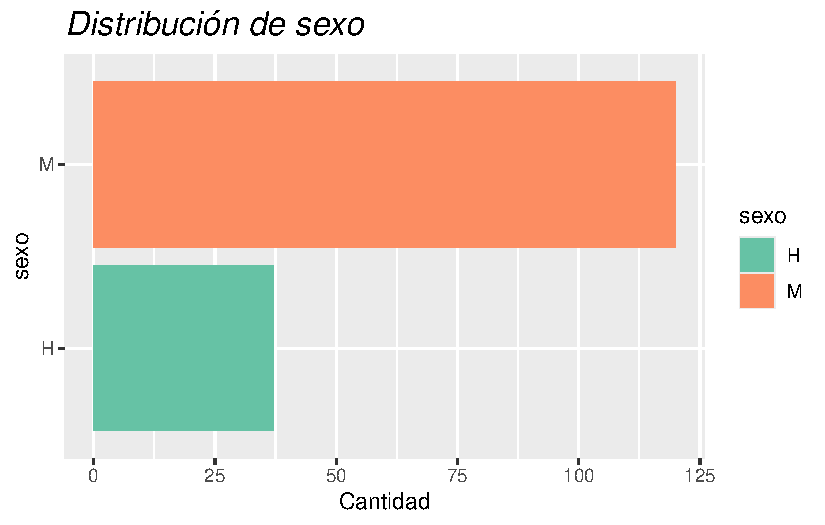
\includegraphics[width=0.85\linewidth,height=\textheight,keepaspectratio]{unidad_1/05_intro_ggplot_files/figure-pdf/cod24-1.pdf}
\end{center}

\section{\texorpdfstring{Paquete
\texttt{esquisse}}{Paquete esquisse}}\label{paquete-esquisse}

\begin{center}

\includegraphics[width=0.2\linewidth,height=\textheight,keepaspectratio]{bg_images/esquisse.PNG}
\end{center}

El paquete\texttt{esquisse} (Meyer y Perrier 2025) es una extensión de
\texttt{ggplot2} que permite crear gráficos de manera interactiva,
mediante una interfaz gráfica intuitiva basada en el sistema de
arrastrar y soltar (\emph{drag \& drop}).

Con \texttt{esquisse} es posible:

\begin{itemize}
\item
  Explorar visualmente los datos según su tipo.
\item
  Asignar variables a diferentes estéticas del gráfico (ejes, color,
  tamaño, etc.).
\item
  Exportar los resultados en distintos formatos.
\item
  Recuperar el código R que genera el gráfico, facilitando su
  reproducción y modificación.
\end{itemize}

El paquete se instala mediante el menú \textbf{Packages} de RStudio o
ejecutando:

\begin{Shaded}
\begin{Highlighting}[]
\FunctionTok{install.packages}\NormalTok{(}\StringTok{"esquisse"}\NormalTok{)}
\end{Highlighting}
\end{Shaded}

Luego se puede acceder a la aplicación por medio del acceso Addins:

\begin{center}
\pandocbounded{
\includegraphics[keepaspectratio]{unidad_1/images/addins.png}}
\end{center}

o ejecutando en consola:

\begin{Shaded}
\begin{Highlighting}[]
\FunctionTok{esquisser}\NormalTok{()}
\end{Highlighting}
\end{Shaded}

También se puede agregar el nombre de la tabla de datos dentro de los
paréntesis

\begin{Shaded}
\begin{Highlighting}[]
\FunctionTok{esquisser}\NormalTok{(datos)}
\end{Highlighting}
\end{Shaded}

Para más detalles, se puede consultar la
\href{https://cran.r-project.org/web/packages/esquisse/vignettes/get-started.html}{viñeta}
del paquete disponible en CRAN o en su
\href{https://github.com/dreamRs/esquisse}{repositorio de GitHub}.

\section{\texorpdfstring{Extensiones de
\texttt{ggplot2}}{Extensiones de ggplot2}}\label{extensiones-de-ggplot2}

Una de las grandes fortalezas de \texttt{ggplot2} es su ecosistema de
extensiones. Hasta el momento, existen más de
\href{https://exts.ggplot2.tidyverse.org/gallery/}{158}
\href{https://exts.ggplot2.tidyverse.org/gallery/}{\textbf{paquetes}}
desarrollados para ampliar sus funcionalidades, muchos de ellos
diseñados para facilitar tareas específicas o agregar nuevas capas,
geometrías, temas, escalas o herramientas interactivas.

Algunas de las extensiones que utilizaremos durante el curso son:

\begin{itemize}
\item
  \texttt{patchwork} (Pedersen 2025): permite combinar múltiples
  gráficos de \texttt{ggplot2} en una misma figura de forma sencilla y
  controlada.
\item
  \texttt{GGally} (Schloerke et~al. 2025): extiende \texttt{ggplot2} con
  funciones para crear matrices de gráficos (como \texttt{ggpairs()}),
  útiles para análisis exploratorio multivariado.
\item
  \texttt{ggpubr} (Kassambara 2026a): facilita la creación de gráficos
  listos para publicar, con funciones simplificadas para agregar
  títulos, etiquetas, comparaciones estadísticas y anotaciones.
\item
  \texttt{see} (Lüdecke et~al. 2021): ofrece temas, paletas de colores y
  escalas compatibles con personas con daltonismo, además de geometrías
  personalizadas.
\item
  \texttt{survminer}(Kassambara et~al. 2026): diseñado para la
  visualización de análisis de supervivencia (como curvas de
  Kaplan-Meier) utilizando \texttt{ggplot2}.
\item
  \texttt{ggfortify}(Horikoshi y Tang 2018): permite graficar objetos
  estadísticos como modelos lineales, PCA o series temporales sin
  necesidad de escribir código \texttt{ggplot2} desde cero.
\end{itemize}

Estas extensiones permiten ampliar la flexibilidad y expresividad
gráfica de \texttt{ggplot2} sin perder la estructura gramatical que lo
caracteriza.

\section*{Referencias}\label{referencias-2}
\addcontentsline{toc}{section}{Referencias}

\markright{Referencias}

\chapter{Análisis exploratorio de
datos}\label{anuxe1lisis-exploratorio-de-datos}

\begin{center}

\includegraphics[width=0.44\linewidth,height=\textheight,keepaspectratio]{bg_images/EDA_packages.png}
\end{center}

\section{Introducción}\label{introducciuxf3n-3}

El análisis exploratorio de datos (conocido como \textbf{EDA}, su sigla
en inglés) es un enfoque de análisis fundamental para resumir y
visualizar las características importantes de un conjunto de datos.

\href{https://es.wikipedia.org/wiki/John_W._Tukey}{\textbf{John Tukey}},
estadístico estadounidense, fue uno de los principales impulsores de
este enfoque. En 1977 publicó el libro \emph{Exploratory Data Analysis},
donde, entre otras contribuciones, introdujo el gráfico \emph{boxplot}
(diagrama de caja y bigotes).

En términos sencillos, antes de avanzar hacia el análisis formal o la
construcción de modelos estadísticos, resulta esencial explorar, conocer
y describir las variables presentes en nuestra tabla de datos.

Entre los principales objetivos perseguidos por EDA se encuentran:

\begin{itemize}
\tightlist
\item
  Conocer la estructura de la tabla de datos y sus tipos de variable.
\item
  Detectar observaciones incompletas (valores \emph{missing} o
  \texttt{NA}).
\item
  Explorar la distribución de las variables de interés a partir de:

  \begin{itemize}
  \tightlist
  \item
    Estadísticos descriptivos
  \item
    Representaciones gráficas
  \end{itemize}
\item
  Detectar valores atípicos (\emph{outliers}).
\end{itemize}

\subsubsection{Aclaración}\label{aclaraciuxf3n}

En este documento utilizaremos funciones del lenguaje R basadas en la
filosofía \emph{tidyverse}, junto con otros paquetes diseñados para
tareas específicas. Esto no implica que no se puedan emplear funciones
del R base; sin embargo, el ecosistema \texttt{tidyverse} facilita la
comprensión y legibilidad del código.

Presentaremos estas diferentes funciones de distintos paquetes que
pueden servir en cada etapa de un EDA. Los paquetes con los que
trabajaremos son:

\begin{itemize}
\tightlist
\item
  \texttt{tidyverse}
\item
  \texttt{skimr}
\item
  \texttt{dlookr}
\item
  \texttt{janitor}
\end{itemize}

\begin{tcolorbox}[enhanced jigsaw, arc=.35mm, bottomrule=.15mm, breakable, colback=white, colframe=quarto-callout-warning-color-frame, left=2mm, leftrule=.75mm, opacityback=0, rightrule=.15mm, toprule=.15mm]
\begin{minipage}[t]{5.5mm}
\textcolor{quarto-callout-warning-color}{\faExclamationTriangle}
\end{minipage}%
\begin{minipage}[t]{\textwidth - 5.5mm}

\textbf{Nota:} Algunos paquetes, como \texttt{dlookr}, pueden generar
falsos positivos en la detección del antivirus durante el proceso de
instalación. Sugerimos desactivar momentáneamente el antivirus para
evitar inconvenientes.

\end{minipage}%
\end{tcolorbox}

Una vez instalados, podemos activar los paquetes con el siguiente
código:

\begin{Shaded}
\begin{Highlighting}[]
\CommentTok{\# Carga de paquetes}
\FunctionTok{library}\NormalTok{(skimr)}
\FunctionTok{library}\NormalTok{(janitor)}
\FunctionTok{library}\NormalTok{(dlookr)}
\FunctionTok{library}\NormalTok{(tidyverse)}
\end{Highlighting}
\end{Shaded}

Se recomienda cargar \texttt{tidyverse} al final de la lista para evitar
conflictos con funciones que puedan solaparse entre paquetes.

\begin{quote}
Es importante destacar que no existe un único camino y/o función para
realizar un análisis exploratorio. Esta selección de herramientas puede
adaptarse según las preferencias y necesidades de cada usuario. Por lo
tanto, quienes ya tengan familiaridad con otras funciones o paquetes
pueden continuar utilizándolos sin inconvenientes.
\end{quote}

Para ilustrar los pasos del análisis exploratorio, utilizaremos un
archivo con datos ficticios llamado ``\texttt{datos2.txt}'', que
contiene variables de distintos tipos.

\section{Conocer la estructura de la tabla de datos y sus tipos de
variable}\label{conocer-la-estructura-de-la-tabla-de-datos-y-sus-tipos-de-variable}

El primer paso en la exploración de un conjunto de datos es conocer su
estructura y tamaño:

\begin{itemize}
\item
  El \textbf{tamaño} se refiere a la cantidad de observaciones (filas) y
  de variables (columnas).
\item
  La \textbf{estructura} incluye cómo están organizadas las variables,
  qué tipo de datos contiene cada una y qué categorías o valores pueden
  tomar.
\end{itemize}

Comenzaremos por cargar los datos de ejemplo con la función
\texttt{read\_csv2()} de \texttt{tidyverse}:

\begin{Shaded}
\begin{Highlighting}[]
\NormalTok{datos }\OtherTok{\textless{}{-}} \FunctionTok{read\_csv2}\NormalTok{(}\StringTok{"datos/datos2.txt"}\NormalTok{)}
\end{Highlighting}
\end{Shaded}

Una vez cargados los datos, la función \texttt{glimpse()} permite
obtener una visión general de la tabla:

\begin{Shaded}
\begin{Highlighting}[]
\FunctionTok{glimpse}\NormalTok{(datos)}
\end{Highlighting}
\end{Shaded}

\begin{verbatim}
Rows: 74
Columns: 7
$ id      <dbl> 1, 2, 3, 4, 5, 6, 7, 8, 9, 10, 11, 12, 13, 14, 15, 16, 17, 18,~
$ sexo    <chr> "M", "M", "M", "M", "M", "M", "M", "M", NA, "F", "F", "M", "F"~
$ edad    <dbl> 76, 68, 50, 49, 51, 68, 70, 64, 60, 57, 83, 76, 27, 34, 17, 45~
$ peso    <dbl> 71.0, 71.0, 79.0, 71.0, 87.0, 75.0, 80.0, 83.0, 69.0, 73.0, 60~
$ talla   <dbl> 167.0, 164.0, 164.0, 164.0, 167.5, 170.0, 166.0, 160.0, 160.0,~
$ trabaja <lgl> FALSE, FALSE, FALSE, TRUE, TRUE, FALSE, NA, TRUE, TRUE, TRUE, ~
$ fecha   <chr> "20/10/2020", "20/10/2020", "20/10/2020", "05/11/2020", "05/11~
\end{verbatim}

Esta función nos informa que la tabla contiene, por ejemplo, 74
observaciones y 7 variables, mostrando el tipo de dato de cada una y los
primeros valores que aparecen.

Entre los tipos de datos más comunes que podemos encontrar se incluyen:

\begin{itemize}
\item
  \texttt{int} (\emph{integer}): números enteros.
\item
  \texttt{dbl} (\emph{double}): números reales.
\item
  \texttt{lgl} (\emph{logical}): valores lógicos (\texttt{TRUE},
  \texttt{FALSE}).
\item
  \texttt{chr} (\emph{character}): texto o cadenas de caracteres.
\item
  \texttt{Date}: fechas.
\item
  \texttt{fct} (\emph{factor}): variables categóricas con niveles.
\item
  \texttt{dttm} (\emph{date-time}): fechas y horas.
\end{itemize}

Esta primera revisión de la estructura suele complementarse con el
\textbf{diccionario de datos}, un recurso fundamental que describe el
significado, tipo, unidad y codificación de cada variable. Este
diccionario puede acompañar tanto a bases de datos generadas en
investigaciones propias (fuentes primarias) como a datos provenientes de
fuentes secundarias.

Es importante tener en cuenta que el tipo de dato en R no siempre
coincide con la naturaleza estadística de la variable. Por ejemplo:

\begin{itemize}
\item
  Una variable codificada como \texttt{dbl} puede representar una medida
  cuantitativa continua, como la edad o el peso.
\item
  Pero también puede representar una variable cualitativa codificada con
  números. Por ejemplo, si una variable que registra respuestas ``Sí'' y
  ``No'' fue codificada como \texttt{1} y \texttt{0}, su tipo de dato
  será numérico (\texttt{dbl} o \texttt{int}), aunque conceptualmente
  sea una variable categórica.
\end{itemize}

Por esta razón, además de inspeccionar el tipo de datos en R, es
importante revisar el significado y el uso previsto de cada variable
dentro del contexto del análisis.

\section{Detectar observaciones
incompletas}\label{detectar-observaciones-incompletas}

Los valores perdidos o faltantes (conocidos como \emph{missing} en
inglés), representados en R por el valor especial \texttt{NA},
constituyen un desafío importante en el análisis de datos. Su presencia
puede afectar la calidad del análisis y condicionar las decisiones
estadísticas posteriores.

Existen numerosos enfoques para el tratamiento de valores faltantes,
incluyendo técnicas de imputación y modelado específico. Sin embargo, en
este curso nos enfocaremos exclusivamente en cómo \textbf{detectar},
\textbf{contabilizar} y, en algunos casos, \textbf{excluir} valores
faltantes utilizando funciones del lenguaje R.

Una forma sencilla de detectar valores faltantes es mediante la función
\texttt{count()} del paquete \texttt{dplyr}. Al aplicarla a una
variable, la salida incluye una fila adicional que informa cuántos
valores \texttt{NA} hay:

\begin{Shaded}
\begin{Highlighting}[]
\NormalTok{datos }\SpecialCharTok{|\textgreater{}}
  \FunctionTok{count}\NormalTok{(trabaja)}
\end{Highlighting}
\end{Shaded}

\begin{verbatim}
# A tibble: 3 x 2
  trabaja     n
  <lgl>   <int>
1 FALSE      26
2 TRUE       39
3 NA          9
\end{verbatim}

Una alternativa más completa es la función \texttt{find\_na()} del
paquete \texttt{dlookr} (Ryu 2025):

\begin{Shaded}
\begin{Highlighting}[]
\FunctionTok{find\_na}\NormalTok{(datos, }\AttributeTok{rate =}\NormalTok{ T)}
\end{Highlighting}
\end{Shaded}

\begin{verbatim}
     id    sexo    edad    peso   talla trabaja   fecha 
  0.000   4.054   0.000   0.000   0.000  12.162   0.000 
\end{verbatim}

Esta función se puede aplicar al conjunto de datos completo y devuelve,
para cada variable, la cantidad y el porcentaje de valores \texttt{NA}.
Por ejemplo, podríamos observar que la variable \texttt{sexo} tiene
alrededor de un 4\,\% de valores faltantes, y la variable
\texttt{trabaja}, algo más del 12\,\%.

Estos porcentajes pueden ayudarnos a decidir si una variable debe
incluirse en un análisis o si es conveniente excluir ciertas
observaciones con datos incompletos, siempre que los \texttt{NA} sean el
resultado de una ausencia real de información.

El mismo paquete trae una función gráfica llamada
\texttt{plot\_na\_pareto()}, que genera un gráfico de barras ordenados
por frecuencia de valores faltantes:

\begin{Shaded}
\begin{Highlighting}[]
\FunctionTok{plot\_na\_pareto}\NormalTok{(datos, }\AttributeTok{only\_na =}\NormalTok{ T)}
\end{Highlighting}
\end{Shaded}

\begin{center}
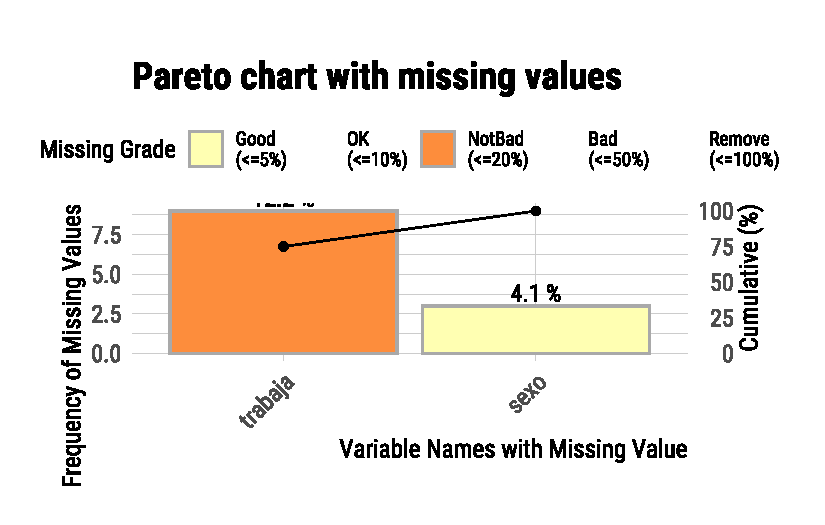
\includegraphics[width=0.85\linewidth,height=\textheight,keepaspectratio]{unidad_1/06_analisis_exploratorio_files/figure-pdf/cod6-1.pdf}
\end{center}

Finalmente, para un diagnóstico más integral de la calidad de las
variables, puede utilizarse la función \texttt{diagnose()}:

\begin{Shaded}
\begin{Highlighting}[]
\FunctionTok{diagnose}\NormalTok{(datos)}
\end{Highlighting}
\end{Shaded}

\begin{verbatim}
# A tibble: 7 x 6
  variables types     missing_count missing_percent unique_count unique_rate
  <chr>     <chr>             <int>           <dbl>        <int>       <dbl>
1 id        numeric               0            0              74      1     
2 sexo      character             3            4.05            3      0.0405
3 edad      numeric               0            0              45      0.608 
4 peso      numeric               0            0              56      0.757 
5 talla     numeric               0            0              38      0.514 
6 trabaja   logical               9           12.2             3      0.0405
7 fecha     character             0            0              11      0.149 
\end{verbatim}

Esta función ofrece un resumen detallado que incluye el tipo de
variable, la cantidad de valores faltantes, la proporción de valores
únicos, entre otros indicadores de utilidad para la exploración inicial.

\section{Conocer la distribución de las variables de
interés}\label{conocer-la-distribuciuxf3n-de-las-variables-de-interuxe9s}

\subsection{Resumir variables
cuantitativas}\label{resumir-variables-cuantitativas}

La instalación básica de R tiene incorporadas múltiples funciones
estadísticas que permiten calcular medidas resumen para variables
cuantitativas. Estas funciones pueden integrarse a la función
\texttt{summarise()} de \texttt{tidyverse}.

\subsubsection{Medidas de tendencia
central}\label{medidas-de-tendencia-central}

Las medidas de tendencia central forman parte del grupo de medidas de
posición o localización, pero su objetivo principal es resumir la
información en torno a un valor que representa el ``centro'' de la
distribución. Es decir, un valor respecto al cual tienden a agruparse
los demás valores.

Podemos obtener la media y la mediana de nuestros datos con el siguiente
código:

\begin{Shaded}
\begin{Highlighting}[]
\NormalTok{datos }\SpecialCharTok{|\textgreater{}}
  \FunctionTok{summarise}\NormalTok{(}
    \CommentTok{\# Media}
    \AttributeTok{media =} \FunctionTok{mean}\NormalTok{(edad),}
    \CommentTok{\# Mediana}
    \AttributeTok{mediana =} \FunctionTok{median}\NormalTok{(edad)}
\NormalTok{  )}
\end{Highlighting}
\end{Shaded}

\begin{verbatim}
# A tibble: 1 x 2
  media mediana
  <dbl>   <dbl>
1  48.1    52.5
\end{verbatim}

En cambio, R base no incluye una función específica para calcular la
\textbf{moda}. Para obtenerla, debemos escribir una función propia o
utilizar algún paquete adicional que la implemente (por ejemplo,
\texttt{modeest::mlv()}).

\subsubsection{Medidas de posición}\label{medidas-de-posiciuxf3n}

Las medidas de posición dividen los datos en grupos con igual número de
observaciones. Entre las más utilizadas se encuentran los
\textbf{cuartiles} y \textbf{percentiles}.

La función \texttt{quantile()} del paquete base \texttt{stats} permite
calcular cuartiles u otros percentiles. Por ejemplo, para calcular los
cuartiles Q1 y Q3, indicamos en el argumento \texttt{probs} los valores
0.25 y 0.75:

\begin{Shaded}
\begin{Highlighting}[]
\NormalTok{datos }\SpecialCharTok{|\textgreater{}}
  \FunctionTok{summarise}\NormalTok{(}
    \CommentTok{\# Primer cuartil}
    \AttributeTok{cuartil1 =} \FunctionTok{quantile}\NormalTok{(edad, }\AttributeTok{probs =} \FloatTok{0.25}\NormalTok{),}
    \CommentTok{\# Tercer cuartil}
    \AttributeTok{cuartil3 =} \FunctionTok{quantile}\NormalTok{(edad, }\AttributeTok{probs =} \FloatTok{0.75}\NormalTok{)}
\NormalTok{  )}
\end{Highlighting}
\end{Shaded}

\begin{verbatim}
# A tibble: 1 x 2
  cuartil1 cuartil3
     <dbl>    <dbl>
1       28       64
\end{verbatim}

Para obtener el mínimo y máximo de estos valores numéricos usamos el
siguiente código:

\begin{Shaded}
\begin{Highlighting}[]
\NormalTok{datos }\SpecialCharTok{|\textgreater{}}
  \FunctionTok{summarise}\NormalTok{(}
    \CommentTok{\# Mínimo}
    \AttributeTok{minimo =} \FunctionTok{min}\NormalTok{(edad),}
    \CommentTok{\# Máximo}
    \AttributeTok{maximo =} \FunctionTok{max}\NormalTok{(edad)}
\NormalTok{  )}
\end{Highlighting}
\end{Shaded}

\begin{verbatim}
# A tibble: 1 x 2
  minimo maximo
   <dbl>  <dbl>
1     13     86
\end{verbatim}

\subsubsection{Medidas de dispersión}\label{medidas-de-dispersiuxf3n}

Las medidas de dispersión nos permiten conocer cuán dispersos o
variables son los valores dentro del conjunto de datos.

Entre las más clásicas se encuentran la \textbf{varianza} y el
\textbf{desvío estándar}, que se calculan fácilmente con las funciones
\texttt{var()} y \texttt{sd()}:

\begin{Shaded}
\begin{Highlighting}[]
\NormalTok{datos }\SpecialCharTok{|\textgreater{}}
  \FunctionTok{summarise}\NormalTok{(}
    \CommentTok{\# Varianza}
    \AttributeTok{varianza =} \FunctionTok{var}\NormalTok{(edad),}
    \CommentTok{\# Desvío estándar}
    \AttributeTok{desvio =} \FunctionTok{sd}\NormalTok{(edad)}
\NormalTok{  )}
\end{Highlighting}
\end{Shaded}

\begin{verbatim}
# A tibble: 1 x 2
  varianza desvio
     <dbl>  <dbl>
1     405.   20.1
\end{verbatim}

También puede ser útil calcular el \textbf{rango}, que se obtiene como
la diferencia entre el valor máximo y el mínimo, y el \textbf{rango
intercuartílico (RIC)}, mediante \texttt{IQR()}:

\begin{Shaded}
\begin{Highlighting}[]
\NormalTok{datos }\SpecialCharTok{|\textgreater{}}
  \FunctionTok{summarise}\NormalTok{(}
    \CommentTok{\# Rango}
    \AttributeTok{rango =} \FunctionTok{max}\NormalTok{(edad) }\SpecialCharTok{{-}} \FunctionTok{min}\NormalTok{(edad),}
    \CommentTok{\# Rango intercuartílico}
    \AttributeTok{ric =} \FunctionTok{IQR}\NormalTok{(edad)}
\NormalTok{  )}
\end{Highlighting}
\end{Shaded}

\begin{verbatim}
# A tibble: 1 x 2
  rango   ric
  <dbl> <dbl>
1    73    36
\end{verbatim}

El paquete \texttt{dlookr} ofrece la función \texttt{describe()} para
generar un resumen completo de las variables numéricas:

\begin{Shaded}
\begin{Highlighting}[]
\FunctionTok{describe}\NormalTok{(datos, }\SpecialCharTok{{-}}\NormalTok{id)}
\end{Highlighting}
\end{Shaded}

\begin{verbatim}
# A tibble: 3 x 26
  described_variables     n    na  mean    sd se_mean   IQR skewness kurtosis
  <chr>               <int> <int> <dbl> <dbl>   <dbl> <dbl>    <dbl>    <dbl>
1 edad                   74     0  48.1 20.1    2.34  36      -0.211  -1.11  
2 peso                   74     0  72.5 13.2    1.54  17.7     0.145   0.215 
3 talla                  74     0 165.   8.12   0.944  9.75    0.256   0.0363
# i 17 more variables: p00 <dbl>, p01 <dbl>, p05 <dbl>, p10 <dbl>, p20 <dbl>,
#   p25 <dbl>, p30 <dbl>, p40 <dbl>, p50 <dbl>, p60 <dbl>, p70 <dbl>,
#   p75 <dbl>, p80 <dbl>, p90 <dbl>, p95 <dbl>, p99 <dbl>, p100 <dbl>
\end{verbatim}

Esta función puede aplicarse directamente sobre todo el conjunto de
datos. Si bien selecciona automáticamente las variables numéricas, en
este caso estamos excluyendo explícitamente la variable \texttt{id}, ya
que un identificador no tiene interés estadístico.

El resumen que devuelve incluye:

\begin{itemize}
\item
  \texttt{na}: cantidad de observaciones con datos y con \texttt{NA.}
\item
  \texttt{mean}: media aritmética.
\item
  \texttt{sd}: desvío estándar de la media.
\item
  \texttt{se\_mean}: error estándar de la media.
\item
  \texttt{IQR}: rango intercuartílico.
\item
  Medidas de forma como la simetría (\texttt{skewness}) y la curtosis
  (\texttt{kurtosis}).
\item
  Percentiles, incluyendo la mediana (\texttt{P50}) y los cuartiles
  (\texttt{P25} y \texttt{P75}).
\end{itemize}

\subsection{Resumir variables
cualitativas}\label{resumir-variables-cualitativas}

Las variables cualitativas o categóricas pueden encontrarse en R bajo
los tipos de dato \texttt{character} o \texttt{factor}. En ocasiones
será necesario convertirlas a \texttt{factor}, ya que este tipo permite
aplicar ciertos procedimientos específicos para variables categóricas.

\subsubsection{Frecuencias}\label{frecuencias}

Podemos resumir individualmente variables cualitativas mediante las
frecuencias absolutas y relativas de sus categorías. La función
\texttt{count()} de \texttt{dplyr} nos muestra el conteo absoluto:

\begin{Shaded}
\begin{Highlighting}[]
\NormalTok{datos }\SpecialCharTok{|\textgreater{}}
  \FunctionTok{count}\NormalTok{(sexo)}
\end{Highlighting}
\end{Shaded}

\begin{verbatim}
# A tibble: 3 x 2
  sexo      n
  <chr> <int>
1 F        27
2 M        44
3 <NA>      3
\end{verbatim}

En la salida se incluirán, además de las categorías presentes, las
observaciones con valores faltantes (\texttt{NA}).

La inclusión o no de los valores faltantes dependerá del propósito del
análisis. Para excluirlos, podemos utilizar \texttt{drop\_na()}:

\begin{Shaded}
\begin{Highlighting}[]
\NormalTok{datos }\SpecialCharTok{|\textgreater{}}
  \FunctionTok{count}\NormalTok{(sexo) }\SpecialCharTok{|\textgreater{}}
  \CommentTok{\# Saltea los valores NA}
  \FunctionTok{drop\_na}\NormalTok{()}
\end{Highlighting}
\end{Shaded}

\begin{verbatim}
# A tibble: 2 x 2
  sexo      n
  <chr> <int>
1 F        27
2 M        44
\end{verbatim}

Para obtener frecuencias relativas en porcentaje:

\begin{Shaded}
\begin{Highlighting}[]
\NormalTok{datos }\SpecialCharTok{|\textgreater{}}
  \FunctionTok{count}\NormalTok{(sexo) }\SpecialCharTok{|\textgreater{}}
  \CommentTok{\# Saltea los valores NA}
  \FunctionTok{drop\_na}\NormalTok{() }\SpecialCharTok{|\textgreater{}}
  \CommentTok{\# Transforma a porcentajes}
  \FunctionTok{mutate}\NormalTok{(}\AttributeTok{porc =} \DecValTok{100} \SpecialCharTok{*}\NormalTok{ n }\SpecialCharTok{/} \FunctionTok{sum}\NormalTok{(n))}
\end{Highlighting}
\end{Shaded}

\begin{verbatim}
# A tibble: 2 x 3
  sexo      n  porc
  <chr> <int> <dbl>
1 F        27  38.0
2 M        44  62.0
\end{verbatim}

Redondeamos el valor del porcentaje con \texttt{round()}:

\begin{Shaded}
\begin{Highlighting}[]
\NormalTok{datos }\SpecialCharTok{|\textgreater{}}
  \FunctionTok{count}\NormalTok{(sexo) }\SpecialCharTok{|\textgreater{}}
  \CommentTok{\# Saltea los valores NA}
  \FunctionTok{drop\_na}\NormalTok{() }\SpecialCharTok{|\textgreater{}}
  \CommentTok{\# Transforma a porcentajes y redondea decimales}
  \FunctionTok{mutate}\NormalTok{(}
    \AttributeTok{porc =} \DecValTok{100} \SpecialCharTok{*}\NormalTok{ n }\SpecialCharTok{/} \FunctionTok{sum}\NormalTok{(n),}
    \AttributeTok{porc =} \FunctionTok{round}\NormalTok{(porc, }\AttributeTok{digits =} \DecValTok{2}\NormalTok{)}
\NormalTok{  )}
\end{Highlighting}
\end{Shaded}

\begin{verbatim}
# A tibble: 2 x 3
  sexo      n  porc
  <chr> <int> <dbl>
1 F        27  38.0
2 M        44  62.0
\end{verbatim}

El paquete \texttt{janitor} (Firke 2024) ofrece una alternativa más
completa mediante la función \texttt{tabyl()}:

\begin{Shaded}
\begin{Highlighting}[]
\NormalTok{datos }\SpecialCharTok{|\textgreater{}}
  \FunctionTok{tabyl}\NormalTok{(sexo)}
\end{Highlighting}
\end{Shaded}

\begin{verbatim}
 sexo  n    percent valid_percent
    F 27 0.36486486     0.3802817
    M 44 0.59459459     0.6197183
 <NA>  3 0.04054054            NA
\end{verbatim}

Esta función muestra tanto frecuencias absolutas como relativas,
incluyendo y excluyendo los valores \texttt{NA} (porcentaje sobre el
total de valores válidos).

Podemos mejorar la presentación combinando otras funciones del paquete:

\begin{Shaded}
\begin{Highlighting}[]
\NormalTok{datos }\SpecialCharTok{|\textgreater{}}
  \CommentTok{\# Excluímos valores NA}
  \FunctionTok{tabyl}\NormalTok{(sexo, }\AttributeTok{show\_na =}\NormalTok{ F) }\SpecialCharTok{|\textgreater{}}
  \CommentTok{\# Añadimos totales por fila}
  \FunctionTok{adorn\_totals}\NormalTok{(}\AttributeTok{where =} \StringTok{"row"}\NormalTok{) }\SpecialCharTok{|\textgreater{}}
  \CommentTok{\# Redondea porcentajes a 2 decimales}
  \FunctionTok{adorn\_pct\_formatting}\NormalTok{(}\AttributeTok{digits =} \DecValTok{2}\NormalTok{)}
\end{Highlighting}
\end{Shaded}

\begin{verbatim}
  sexo  n percent
     F 27  38.03%
     M 44  61.97%
 Total 71 100.00%
\end{verbatim}

\subsubsection{Tablas de contingencia}\label{tablas-de-contingencia}

La forma más adecuada de describir la relación entre dos variables
cualitativas es a través de una \textbf{tabla de contingencia}, en la
cual:

\begin{itemize}
\item
  Las filas representan las categorías de una variable.
\item
  Las columnas representan las categorías de otra variable.
\item
  Las celdas muestran el número de observaciones correspondientes a cada
  combinación de categorías.
\end{itemize}

La función \texttt{tabyl()} también permite crear este tipo de tablas. A
continuación, un ejemplo entre \texttt{sexo} y \texttt{trabaja} (aunque
\texttt{trabaja} sea lógica, puede tratarse como categórica):

\begin{Shaded}
\begin{Highlighting}[]
\NormalTok{datos }\SpecialCharTok{|\textgreater{}}
  \FunctionTok{tabyl}\NormalTok{(sexo, trabaja)}
\end{Highlighting}
\end{Shaded}

\begin{verbatim}
 sexo FALSE TRUE NA_
    F     8   15   4
    M    17   22   5
 <NA>     1    2   0
\end{verbatim}

Recordemos que el orden dentro de los paréntesis de la función es igual
al de los índices, el primer argumento es la variable que aparecerá en
las filas y el segundo la variable de las columnas. Por ese motivo, en
la tabla de contingencia absoluta tenemos \texttt{sexo} en las filas y
\texttt{trabaja} en las columnas.

Se puede mejorar la tabla excluyendo los valores \texttt{NA} y agregando
totales por fila:

\begin{Shaded}
\begin{Highlighting}[]
\NormalTok{datos }\SpecialCharTok{|\textgreater{}}
  \CommentTok{\# Excluímos valores NA}
  \FunctionTok{tabyl}\NormalTok{(sexo, trabaja, }\AttributeTok{show\_na =}\NormalTok{ F) }\SpecialCharTok{|\textgreater{}}
  \CommentTok{\# Añadimos totales por fila}
  \FunctionTok{adorn\_totals}\NormalTok{(}\AttributeTok{where =} \StringTok{"row"}\NormalTok{)}
\end{Highlighting}
\end{Shaded}

\begin{verbatim}
  sexo FALSE TRUE
     F     8   15
     M    17   22
 Total    25   37
\end{verbatim}

Para calcular frecuencias relativas porcentuales por columna usamos el
siguiente código:

\begin{Shaded}
\begin{Highlighting}[]
\NormalTok{datos }\SpecialCharTok{|\textgreater{}}
  \CommentTok{\# Excluímos valores NA}
  \FunctionTok{tabyl}\NormalTok{(sexo, trabaja, }\AttributeTok{show\_na =}\NormalTok{ F) }\SpecialCharTok{|\textgreater{}}
  \CommentTok{\# Añadimos totales}
  \FunctionTok{adorn\_totals}\NormalTok{(}\AttributeTok{where =} \StringTok{"row"}\NormalTok{) }\SpecialCharTok{|\textgreater{}}
  \CommentTok{\# Añadimos porcentajes por columna}
  \FunctionTok{adorn\_percentages}\NormalTok{(}\AttributeTok{denominator =} \StringTok{"col"}\NormalTok{) }\SpecialCharTok{|\textgreater{}}
  \CommentTok{\# Redondea porcentajes a 2 decimales}
  \FunctionTok{adorn\_pct\_formatting}\NormalTok{(}\AttributeTok{digits =} \DecValTok{2}\NormalTok{)}
\end{Highlighting}
\end{Shaded}

\begin{verbatim}
  sexo   FALSE    TRUE
     F  32.00%  40.54%
     M  68.00%  59.46%
 Total 100.00% 100.00%
\end{verbatim}

Calculamos frecuencias relativas porcentuales por fila:

\begin{Shaded}
\begin{Highlighting}[]
\NormalTok{datos }\SpecialCharTok{|\textgreater{}}
  \CommentTok{\# Excluímos valores NA}
  \FunctionTok{tabyl}\NormalTok{(sexo, trabaja, }\AttributeTok{show\_na =}\NormalTok{ F) }\SpecialCharTok{|\textgreater{}}
  \CommentTok{\# Añadimos totales por columna}
  \FunctionTok{adorn\_totals}\NormalTok{(}\AttributeTok{where =} \StringTok{"col"}\NormalTok{) }\SpecialCharTok{|\textgreater{}}
  \CommentTok{\# Añadimos porcentajes por fila}
  \FunctionTok{adorn\_percentages}\NormalTok{(}\AttributeTok{denominator =} \StringTok{"row"}\NormalTok{) }\SpecialCharTok{|\textgreater{}}
  \CommentTok{\# Redondea porcentajes a 2 decimales}
  \FunctionTok{adorn\_pct\_formatting}\NormalTok{(}\AttributeTok{digits =} \DecValTok{2}\NormalTok{)}
\end{Highlighting}
\end{Shaded}

\begin{verbatim}
 sexo  FALSE   TRUE   Total
    F 34.78% 65.22% 100.00%
    M 43.59% 56.41% 100.00%
\end{verbatim}

Cambiando el argumento \texttt{denominator} por \texttt{"all"} se
calculan frecuencias relativas al total:

\begin{Shaded}
\begin{Highlighting}[]
\NormalTok{datos }\SpecialCharTok{|\textgreater{}}
  \CommentTok{\# Excluímos valores NA}
  \FunctionTok{tabyl}\NormalTok{(sexo, trabaja, }\AttributeTok{show\_na =}\NormalTok{ F) }\SpecialCharTok{|\textgreater{}}
  \CommentTok{\# Añadimos totales por columna}
  \FunctionTok{adorn\_totals}\NormalTok{(}\AttributeTok{where =} \StringTok{"col"}\NormalTok{) }\SpecialCharTok{|\textgreater{}}
  \CommentTok{\# Añadimos porcentajes al total}
  \FunctionTok{adorn\_percentages}\NormalTok{(}\AttributeTok{denominator =} \StringTok{"all"}\NormalTok{) }\SpecialCharTok{|\textgreater{}}
  \CommentTok{\# Redondea porcentajes a 2 decimales}
  \FunctionTok{adorn\_pct\_formatting}\NormalTok{(}\AttributeTok{digits =} \DecValTok{2}\NormalTok{)}
\end{Highlighting}
\end{Shaded}

\begin{verbatim}
 sexo  FALSE   TRUE  Total
    F 12.90% 24.19% 37.10%
    M 27.42% 35.48% 62.90%
\end{verbatim}

\subsection{Explorar variables mediante
gráficos}\label{explorar-variables-mediante-gruxe1ficos}

Uno de los aportes más importantes de John Tukey al análisis de datos es
la incorporación de los gráficos como herramienta exploratoria. A través
de representaciones visuales podemos detectar rápidamente patrones,
anomalías, valores extremos, asimetrías o relaciones entre variables.

En R, los gráficos más útiles para explorar la distribución
\textbf{univariada} de las variables son:

\begin{itemize}
\item
  Para variables \textbf{cualitativas}: gráficos de barras
\item
  Para variables \textbf{cuantitativas}: histogramas, gráficos de
  densidad, boxplots y violin plots
\item
  Cuando queremos explorar la relación entre \textbf{dos o más
  variables}, los tipos de gráficos más comunes incluyen:

  \begin{itemize}
  \item
    Diagramas de dispersión (puntos)
  \item
    Gráficos de líneas
  \item
    Gráficos de mosaico para variables categóricas cruzadas
  \end{itemize}
\end{itemize}

El lenguaje R soporta una serie de sistemas gráficos asociados a
paquetes como \texttt{graphics}, \texttt{lattice}, \texttt{ggplot2},
etc. que sirven de base incluso para otros paquetes con funciones más
específicas. Actualmente el estándar gráfico en R es \texttt{ggplot2}.

\subsubsection{Barras (univariado)}\label{barras-univariado}

El gráfico de barras permite visualizar la frecuencia de las categorías
de una variable cualitativa:

\begin{Shaded}
\begin{Highlighting}[]
\NormalTok{datos }\SpecialCharTok{|\textgreater{}}
  \CommentTok{\# Omitimos los NA de sexo}
  \FunctionTok{drop\_na}\NormalTok{(sexo) }\SpecialCharTok{|\textgreater{}}
  \CommentTok{\# Generamos histograma}
  \FunctionTok{ggplot}\NormalTok{(}\FunctionTok{aes}\NormalTok{(}\AttributeTok{x =}\NormalTok{ sexo, }\AttributeTok{fill =}\NormalTok{ sexo)) }\SpecialCharTok{+}
  \FunctionTok{geom\_bar}\NormalTok{() }\SpecialCharTok{+}
  \FunctionTok{scale\_fill\_manual}\NormalTok{(}\AttributeTok{values =} \FunctionTok{c}\NormalTok{(}\StringTok{"palevioletred4"}\NormalTok{, }\StringTok{"orange"}\NormalTok{)) }\SpecialCharTok{+}
  \FunctionTok{theme\_minimal}\NormalTok{()}
\end{Highlighting}
\end{Shaded}

\begin{center}
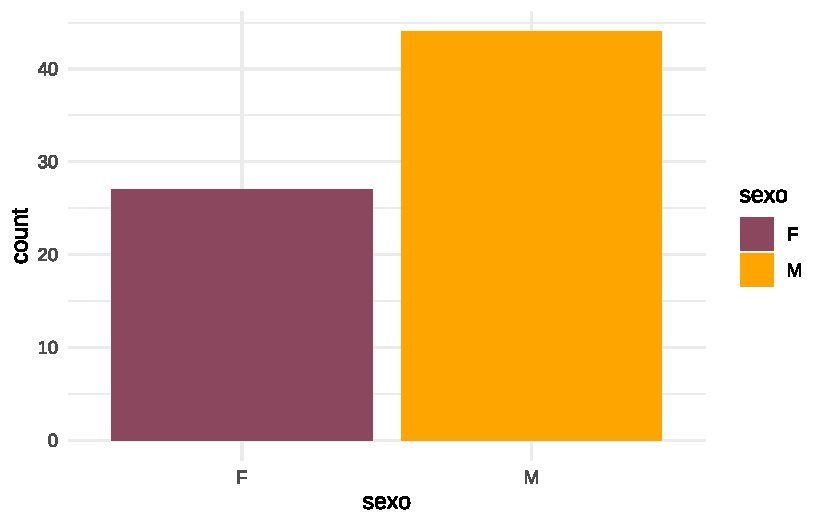
\includegraphics[width=0.85\linewidth,height=\textheight,keepaspectratio]{unidad_1/06_analisis_exploratorio_files/figure-pdf/cod25-1.pdf}
\end{center}

\subsubsection{Barras (bivariado)}\label{barras-bivariado}

Cuando cruzamos dos variables categóricas, podemos representar la
relación entre ambas modificando el argumento \texttt{position} de
\texttt{geom\_bar()}.

El argumento \texttt{position\ =\ "stack"} nos muestra los valores
absolutos acumulados:

\begin{Shaded}
\begin{Highlighting}[]
\NormalTok{datos }\SpecialCharTok{|\textgreater{}}
  \CommentTok{\# Omitimos los NA de sexo y trabaja}
  \FunctionTok{drop\_na}\NormalTok{(sexo, trabaja) }\SpecialCharTok{|\textgreater{}}
  \CommentTok{\# Generamos gráfico de barras}
  \FunctionTok{ggplot}\NormalTok{(}\FunctionTok{aes}\NormalTok{(}\AttributeTok{x =}\NormalTok{ sexo, }\AttributeTok{fill =}\NormalTok{ trabaja)) }\SpecialCharTok{+}
  \FunctionTok{geom\_bar}\NormalTok{(}\AttributeTok{position =} \StringTok{"stack"}\NormalTok{) }\SpecialCharTok{+}
  \FunctionTok{scale\_fill\_brewer}\NormalTok{(}\AttributeTok{palette =} \StringTok{"Set1"}\NormalTok{) }\SpecialCharTok{+}
  \FunctionTok{theme\_minimal}\NormalTok{()}
\end{Highlighting}
\end{Shaded}

\begin{center}
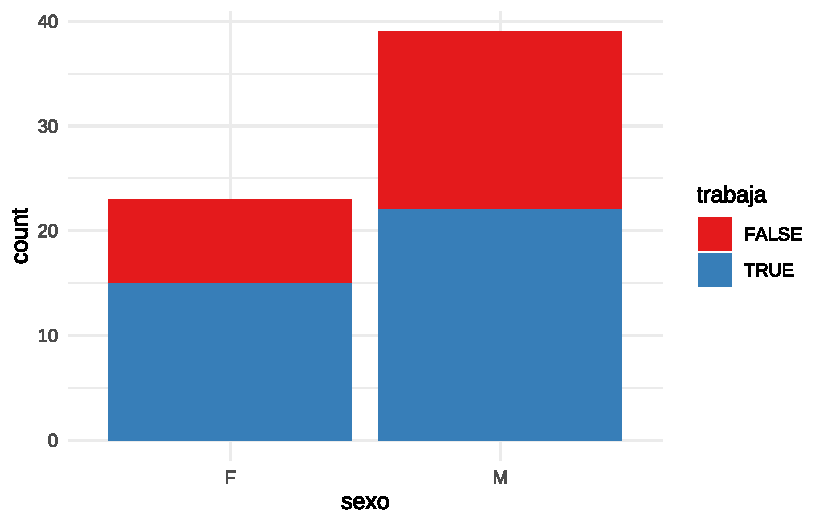
\includegraphics[width=0.85\linewidth,height=\textheight,keepaspectratio]{unidad_1/06_analisis_exploratorio_files/figure-pdf/cod26-1.pdf}
\end{center}

Por otro lado, el argumento \texttt{position\ =\ "dodge"} muestra las
barras lado a lado, permitiendo comparar proporciones entre grupos:

\begin{Shaded}
\begin{Highlighting}[]
\NormalTok{datos }\SpecialCharTok{|\textgreater{}}
  \CommentTok{\# Omitimos los NA de sexo y trabaja}
  \FunctionTok{drop\_na}\NormalTok{(sexo, trabaja) }\SpecialCharTok{|\textgreater{}}
  \CommentTok{\# Generamos gráfico de barras}
  \FunctionTok{ggplot}\NormalTok{(}\FunctionTok{aes}\NormalTok{(}\AttributeTok{x =}\NormalTok{ sexo, }\AttributeTok{fill =}\NormalTok{ trabaja)) }\SpecialCharTok{+}
  \FunctionTok{geom\_bar}\NormalTok{(}\AttributeTok{position =} \StringTok{"dodge"}\NormalTok{) }\SpecialCharTok{+}
  \FunctionTok{scale\_fill\_brewer}\NormalTok{(}\AttributeTok{palette =} \StringTok{"Set1"}\NormalTok{) }\SpecialCharTok{+}
  \FunctionTok{theme\_minimal}\NormalTok{()}
\end{Highlighting}
\end{Shaded}

\begin{center}
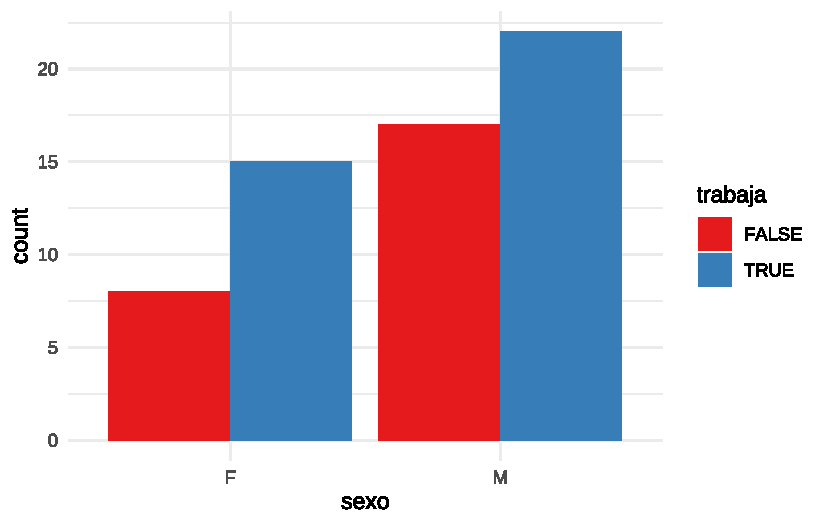
\includegraphics[width=0.85\linewidth,height=\textheight,keepaspectratio]{unidad_1/06_analisis_exploratorio_files/figure-pdf/cod27-1.pdf}
\end{center}

Finalmente, \texttt{position\ =\ "fill"} convierte las alturas en
proporciones sobre el total por grupo:

\begin{Shaded}
\begin{Highlighting}[]
\NormalTok{datos }\SpecialCharTok{|\textgreater{}}
  \CommentTok{\# Omitimos los NA de sexo y trabaja}
  \FunctionTok{drop\_na}\NormalTok{(sexo, trabaja) }\SpecialCharTok{|\textgreater{}}
  \CommentTok{\# Generamos gráfico de barras}
  \FunctionTok{ggplot}\NormalTok{(}\FunctionTok{aes}\NormalTok{(}\AttributeTok{x =}\NormalTok{ sexo, }\AttributeTok{fill =}\NormalTok{ trabaja)) }\SpecialCharTok{+}
  \FunctionTok{geom\_bar}\NormalTok{(}\AttributeTok{position =} \StringTok{"fill"}\NormalTok{) }\SpecialCharTok{+}
  \FunctionTok{scale\_fill\_brewer}\NormalTok{(}\AttributeTok{palette =} \StringTok{"Set1"}\NormalTok{) }\SpecialCharTok{+}
  \FunctionTok{theme\_minimal}\NormalTok{()}
\end{Highlighting}
\end{Shaded}

\begin{center}
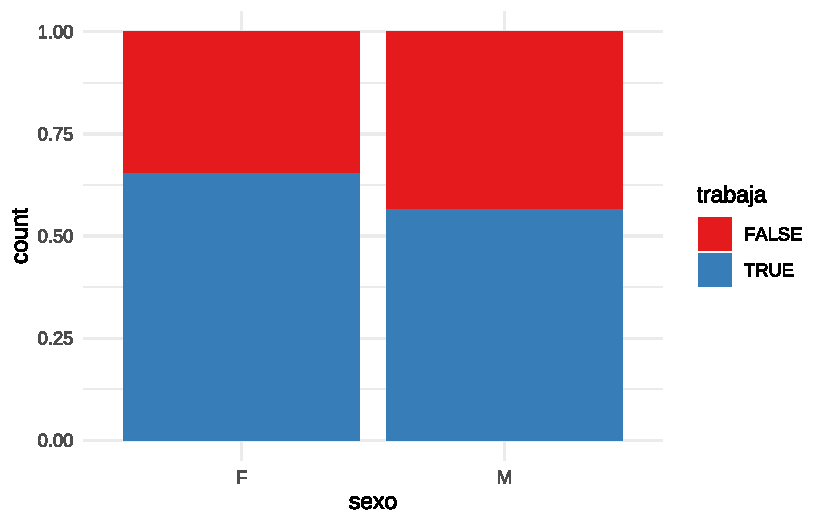
\includegraphics[width=0.85\linewidth,height=\textheight,keepaspectratio]{unidad_1/06_analisis_exploratorio_files/figure-pdf/cod28-1.pdf}
\end{center}

\subsubsection{Histograma}\label{histograma}

Representa la frecuencia de valores en intervalos definidos. Útil para
observar la forma general de la distribución:

\begin{Shaded}
\begin{Highlighting}[]
\NormalTok{datos }\SpecialCharTok{|\textgreater{}}
  \CommentTok{\# Genera histograma}
  \FunctionTok{ggplot}\NormalTok{(}\FunctionTok{aes}\NormalTok{(}\AttributeTok{x =}\NormalTok{ edad)) }\SpecialCharTok{+}
  \FunctionTok{geom\_histogram}\NormalTok{(}\AttributeTok{binwidth =} \DecValTok{10}\NormalTok{, }\AttributeTok{fill =} \StringTok{"royalblue1"}\NormalTok{, }\AttributeTok{color =} \StringTok{"white"}\NormalTok{)}
\end{Highlighting}
\end{Shaded}

\begin{center}
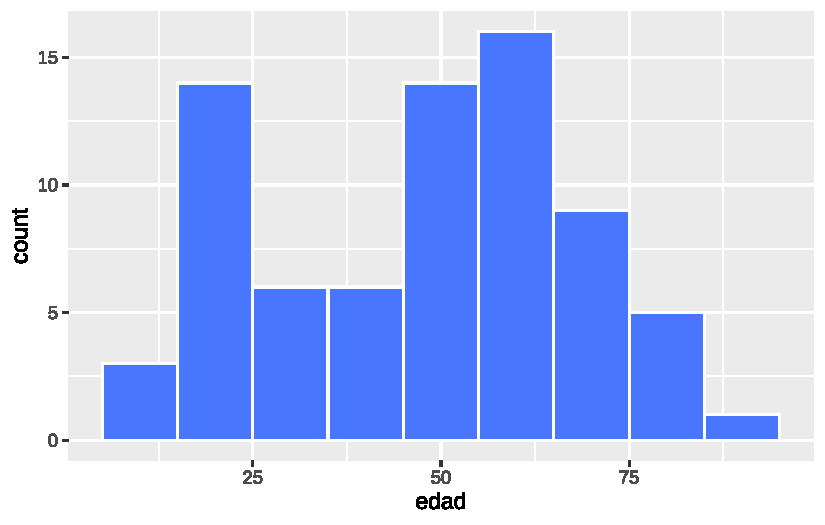
\includegraphics[width=0.85\linewidth,height=\textheight,keepaspectratio]{unidad_1/06_analisis_exploratorio_files/figure-pdf/cod29-1.pdf}
\end{center}

\subsubsection{Densidad}\label{densidad}

Es una estimación suave de la distribución de frecuencias:

\begin{Shaded}
\begin{Highlighting}[]
\NormalTok{datos }\SpecialCharTok{|\textgreater{}}
  \FunctionTok{ggplot}\NormalTok{(}\FunctionTok{aes}\NormalTok{(}\AttributeTok{x =}\NormalTok{ edad)) }\SpecialCharTok{+}
  \FunctionTok{geom\_density}\NormalTok{(}\AttributeTok{fill =} \StringTok{"thistle1"}\NormalTok{)}
\end{Highlighting}
\end{Shaded}

\begin{center}
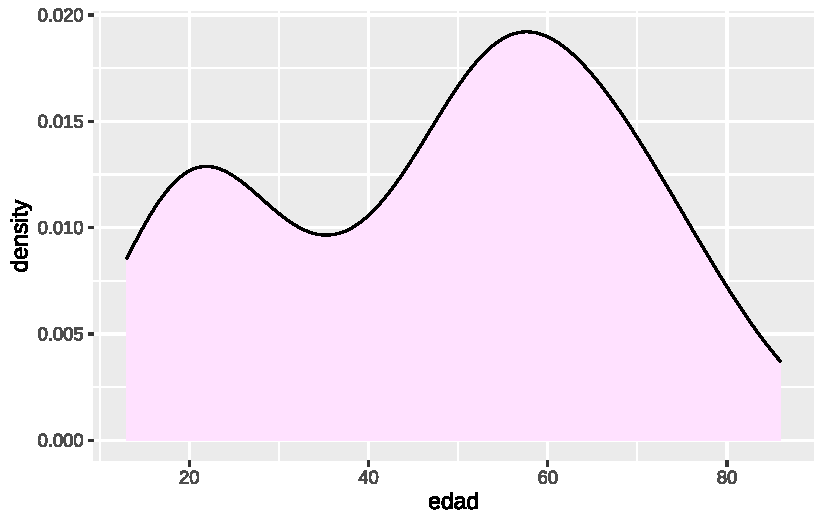
\includegraphics[width=0.85\linewidth,height=\textheight,keepaspectratio]{unidad_1/06_analisis_exploratorio_files/figure-pdf/cod30-1.pdf}
\end{center}

\subsubsection{\texorpdfstring{\emph{Boxplot}}{Boxplot}}\label{boxplot}

Muestra el rango intercuartílico, la mediana y los valores atípicos.
Ideal para detectar asimetrías y \emph{outliers}:

\begin{Shaded}
\begin{Highlighting}[]
\NormalTok{datos }\SpecialCharTok{|\textgreater{}}
  \CommentTok{\# Genera boxplot}
  \FunctionTok{ggplot}\NormalTok{(}\FunctionTok{aes}\NormalTok{(}\AttributeTok{x =}\NormalTok{ edad)) }\SpecialCharTok{+}
  \FunctionTok{geom\_boxplot}\NormalTok{(}\AttributeTok{fill =} \StringTok{"seagreen4"}\NormalTok{)}
\end{Highlighting}
\end{Shaded}

\begin{center}
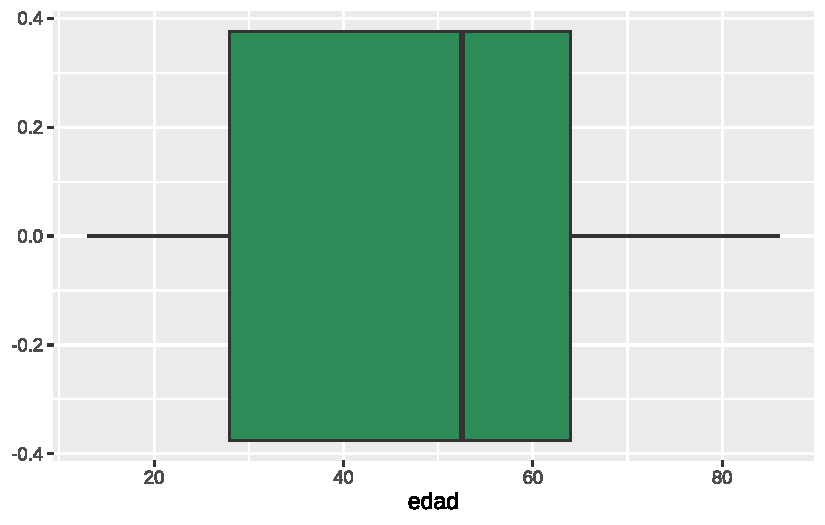
\includegraphics[width=0.85\linewidth,height=\textheight,keepaspectratio]{unidad_1/06_analisis_exploratorio_files/figure-pdf/cod31-1.pdf}
\end{center}

\subsubsection{\texorpdfstring{\emph{Violinplot}}{Violinplot}}\label{violinplot}

Combina el \emph{boxplot} con una curva de densidad reflejada. Permite
visualizar tanto la forma de la distribución como los cuantiles:

\begin{Shaded}
\begin{Highlighting}[]
\NormalTok{datos }\SpecialCharTok{|\textgreater{}}
  \CommentTok{\# Omitimos los NA de sexo}
  \FunctionTok{drop\_na}\NormalTok{(sexo) }\SpecialCharTok{|\textgreater{}}
  \CommentTok{\# Genera violinplot}
  \FunctionTok{ggplot}\NormalTok{(}\FunctionTok{aes}\NormalTok{(}\AttributeTok{x =}\NormalTok{ edad, }\AttributeTok{y =}\NormalTok{ sexo, }\AttributeTok{fill =}\NormalTok{ sexo)) }\SpecialCharTok{+}
  \FunctionTok{geom\_violin}\NormalTok{() }\SpecialCharTok{+}
  \FunctionTok{scale\_fill\_brewer}\NormalTok{(}\AttributeTok{palette =} \StringTok{"Set2"}\NormalTok{) }\SpecialCharTok{+}
  \FunctionTok{theme\_light}\NormalTok{()}
\end{Highlighting}
\end{Shaded}

\begin{center}
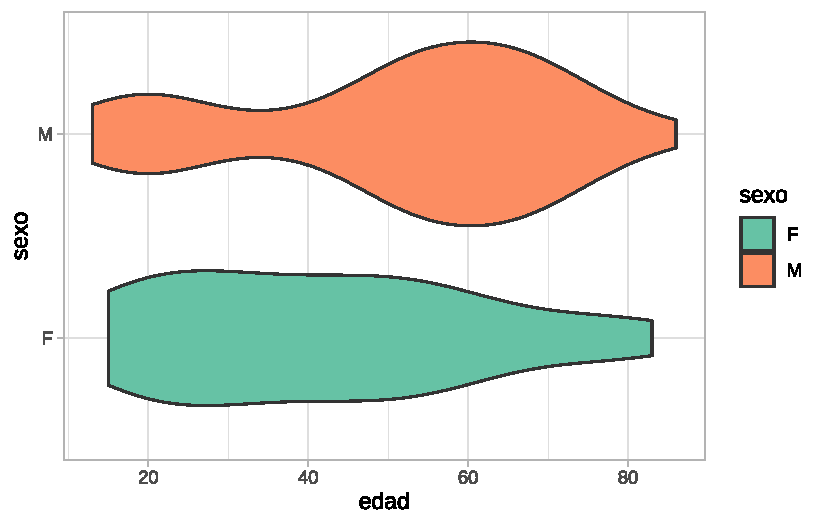
\includegraphics[width=0.85\linewidth,height=\textheight,keepaspectratio]{unidad_1/06_analisis_exploratorio_files/figure-pdf/cod32-1.pdf}
\end{center}

\textbf{\emph{Q-Q Plot}}

Los gráficos Q-Q (cuantil-cuantil) permiten evaluar visualmente si una
variable sigue una distribución teórica, como la normal. Suelen usarse
como método gráfico para analizar ``normalidad'', es decir cuanto se
asemeja la distribución de la variable a la distribución normal o
gaussiana.

La función \texttt{plot\_normality()} de \texttt{dlookr} muestra un
diagnóstico gráfico de normalidad de una variable usando histogramas y
Q-Q plot. Además muestra otros histogramas con conversiones de datos
(logarítmico y raíz cuadrada por defecto, pero también ``Box-Cox'' y
otras):

\begin{Shaded}
\begin{Highlighting}[]
\CommentTok{\# Sobre la variable edad}
\NormalTok{datos }\SpecialCharTok{|\textgreater{}}
  \FunctionTok{plot\_normality}\NormalTok{(edad)}
\end{Highlighting}
\end{Shaded}

\begin{center}
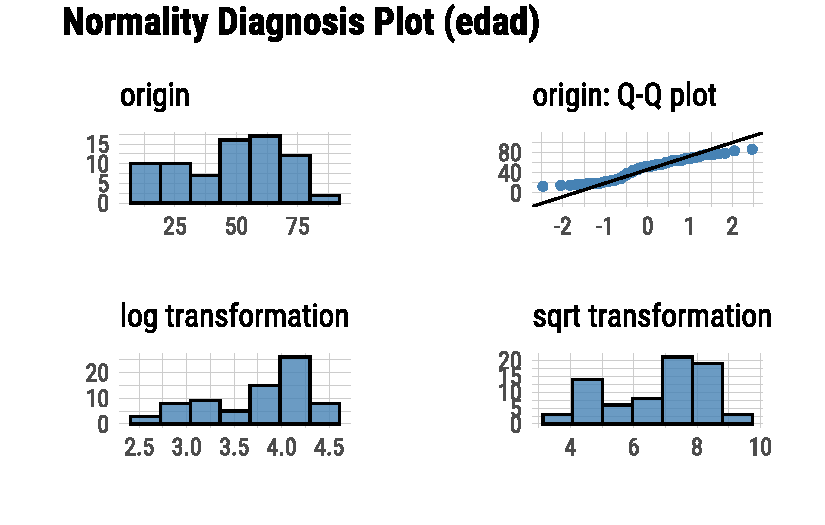
\includegraphics[width=0.85\linewidth,height=\textheight,keepaspectratio]{unidad_1/06_analisis_exploratorio_files/figure-pdf/cod33-1.pdf}
\end{center}

\begin{Shaded}
\begin{Highlighting}[]
\CommentTok{\# Sobre la variable peso}
\NormalTok{datos }\SpecialCharTok{|\textgreater{}}
  \FunctionTok{plot\_normality}\NormalTok{(peso)}
\end{Highlighting}
\end{Shaded}

\begin{center}
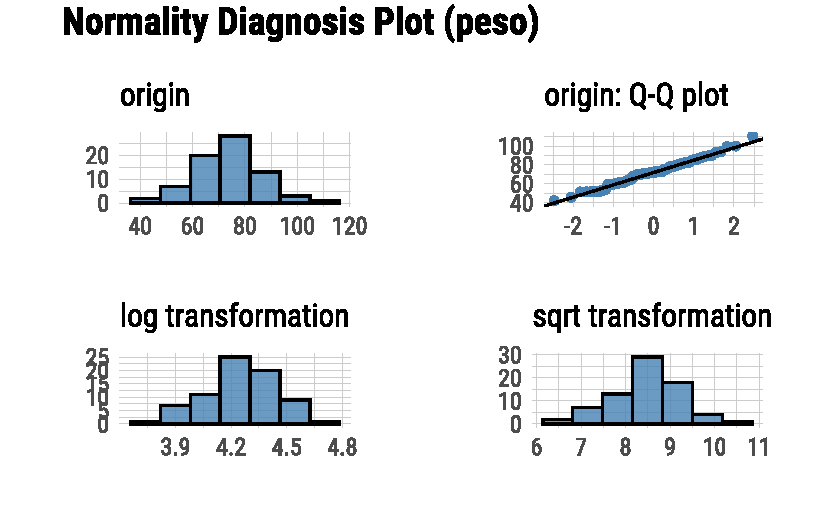
\includegraphics[width=0.85\linewidth,height=\textheight,keepaspectratio]{unidad_1/06_analisis_exploratorio_files/figure-pdf/cod33-2.pdf}
\end{center}

Podemos decir que la variable \texttt{peso} se ajusta mejor a una
distribución normal, ya que los puntos del Q-Q plot se alinean más
cercanamente a la diagonal teórica.

\begin{quote}
\textbf{Nota}: Este análisis gráfico de normalidad suele complementarse
con pruebas estadísticas específicas, que abordaremos en la próxima
unidad.
\end{quote}

\section{Detección de valores
atípicos}\label{detecciuxf3n-de-valores-atuxedpicos}

Un valor atípico (\emph{outlier}) es una observación que se encuentra
numéricamente alejada del resto de los datos. Su presencia puede tener
diferentes causas, y su tratamiento dependerá del contexto:

\begin{itemize}
\item
  \textbf{Errores de carga o procedimiento}: deben corregirse si se
  detectan.
\item
  \textbf{Valores extremos plausibles}: pueden ser válidos, pero
  conviene evaluarlos en detalle.
\item
  \textbf{Eventos extraordinarios o causas desconocidas}: si no se
  pueden justificar, suelen excluirse del análisis.
\end{itemize}

Estos valores pueden afectar sensiblemente ciertos estadísticos como la
media, distorsionando su interpretación.

Una forma gráfica común de detectar valores atípicos es mediante los
\emph{boxplots}. Los puntos situados fuera de los ``bigotes''
representan posibles \emph{outliers}.

A continuación, se presenta un ejemplo con la variable \texttt{peso},
donde se observa un valor extremo en el límite superior de la
distribución (punto rojo):

\begin{Shaded}
\begin{Highlighting}[]
\NormalTok{datos }\SpecialCharTok{|\textgreater{}}
  \FunctionTok{ggplot}\NormalTok{(}\FunctionTok{aes}\NormalTok{(}\AttributeTok{x =}\NormalTok{ peso)) }\SpecialCharTok{+}
  \FunctionTok{geom\_boxplot}\NormalTok{(}\AttributeTok{fill =} \StringTok{"darkkhaki"}\NormalTok{, }\AttributeTok{outlier.color =} \StringTok{"red"}\NormalTok{)}
\end{Highlighting}
\end{Shaded}

\begin{center}
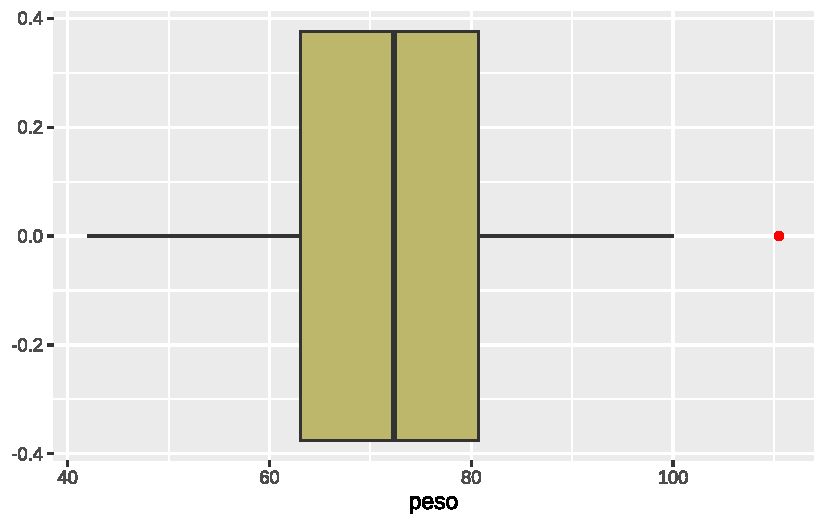
\includegraphics[width=0.85\linewidth,height=\textheight,keepaspectratio]{unidad_1/06_analisis_exploratorio_files/figure-pdf/cod34-1.pdf}
\end{center}

Este valor coincide con el máximo observado:

\begin{Shaded}
\begin{Highlighting}[]
\FunctionTok{max}\NormalTok{(datos}\SpecialCharTok{$}\NormalTok{peso)}
\end{Highlighting}
\end{Shaded}

\begin{verbatim}
[1] 110.5
\end{verbatim}

El paquete \texttt{dlookr} incluye la función
\texttt{diagnose\_outlier()} para la detección automatizada de valores
atípicos en todas las variables numéricas de un conjunto de datos:

\begin{Shaded}
\begin{Highlighting}[]
\FunctionTok{diagnose\_outlier}\NormalTok{(datos)}
\end{Highlighting}
\end{Shaded}

\begin{verbatim}
# A tibble: 4 x 6
  variables outliers_cnt outliers_ratio outliers_mean with_mean without_mean
  <chr>            <int>          <dbl>         <dbl>     <dbl>        <dbl>
1 id                   0           0             NaN       37.5         37.5
2 edad                 0           0             NaN       48.1         48.1
3 peso                 1           1.35          110.      72.5         72.0
4 talla                0           0             NaN      165.         165. 
\end{verbatim}

Esta función devuelve una tabla que incluye, para cada variable:
cantidad y proporción de \emph{outliers} detectados, media de la
variable incluyendo los \emph{outliers}, media de la variable excluyendo
los \emph{outliers}. En función de estos dos estadísticos se puede
comparar el efecto de los valores atípicos en la media.

El paquete \texttt{skimr} (Waring et~al. 2026) permite obtener un
resumen estadístico compacto y amigable de un conjunto de datos mediante
la función \texttt{skim()}:

\begin{Shaded}
\begin{Highlighting}[]
\FunctionTok{skim}\NormalTok{(datos)}
\end{Highlighting}
\end{Shaded}

\begin{longtable}[]{@{}ll@{}}
\caption{Data summary}\tabularnewline
\toprule\noalign{}
\endfirsthead
\endhead
\bottomrule\noalign{}
\endlastfoot
Name & datos \\
Number of rows & 74 \\
Number of columns & 7 \\
\_\_\_\_\_\_\_\_\_\_\_\_\_\_\_\_\_\_\_\_\_\_\_ & \\
Column type frequency: & \\
character & 2 \\
logical & 1 \\
numeric & 4 \\
\_\_\_\_\_\_\_\_\_\_\_\_\_\_\_\_\_\_\_\_\_\_\_\_ & \\
Group variables & None \\
\end{longtable}

\textbf{Variable type: character}

{\def\LTcaptype{none} % do not increment counter
\begin{longtable}[]{@{}
  >{\raggedright\arraybackslash}p{(\linewidth - 14\tabcolsep) * \real{0.1944}}
  >{\raggedleft\arraybackslash}p{(\linewidth - 14\tabcolsep) * \real{0.1389}}
  >{\raggedleft\arraybackslash}p{(\linewidth - 14\tabcolsep) * \real{0.1944}}
  >{\raggedleft\arraybackslash}p{(\linewidth - 14\tabcolsep) * \real{0.0556}}
  >{\raggedleft\arraybackslash}p{(\linewidth - 14\tabcolsep) * \real{0.0556}}
  >{\raggedleft\arraybackslash}p{(\linewidth - 14\tabcolsep) * \real{0.0833}}
  >{\raggedleft\arraybackslash}p{(\linewidth - 14\tabcolsep) * \real{0.1250}}
  >{\raggedleft\arraybackslash}p{(\linewidth - 14\tabcolsep) * \real{0.1528}}@{}}
\toprule\noalign{}
\begin{minipage}[b]{\linewidth}\raggedright
skim\_variable
\end{minipage} & \begin{minipage}[b]{\linewidth}\raggedleft
n\_missing
\end{minipage} & \begin{minipage}[b]{\linewidth}\raggedleft
complete\_rate
\end{minipage} & \begin{minipage}[b]{\linewidth}\raggedleft
min
\end{minipage} & \begin{minipage}[b]{\linewidth}\raggedleft
max
\end{minipage} & \begin{minipage}[b]{\linewidth}\raggedleft
empty
\end{minipage} & \begin{minipage}[b]{\linewidth}\raggedleft
n\_unique
\end{minipage} & \begin{minipage}[b]{\linewidth}\raggedleft
whitespace
\end{minipage} \\
\midrule\noalign{}
\endhead
\bottomrule\noalign{}
\endlastfoot
sexo & 3 & 0.96 & 1 & 1 & 0 & 2 & 0 \\
fecha & 0 & 1.00 & 10 & 10 & 0 & 11 & 0 \\
\end{longtable}
}

\textbf{Variable type: logical}

{\def\LTcaptype{none} % do not increment counter
\begin{longtable}[]{@{}lrrrl@{}}
\toprule\noalign{}
skim\_variable & n\_missing & complete\_rate & mean & count \\
\midrule\noalign{}
\endhead
\bottomrule\noalign{}
\endlastfoot
trabaja & 9 & 0.88 & 0.6 & TRU: 39, FAL: 26 \\
\end{longtable}
}

\textbf{Variable type: numeric}

{\def\LTcaptype{none} % do not increment counter
\begin{longtable}[]{@{}
  >{\raggedright\arraybackslash}p{(\linewidth - 20\tabcolsep) * \real{0.1591}}
  >{\raggedleft\arraybackslash}p{(\linewidth - 20\tabcolsep) * \real{0.1136}}
  >{\raggedleft\arraybackslash}p{(\linewidth - 20\tabcolsep) * \real{0.1591}}
  >{\raggedleft\arraybackslash}p{(\linewidth - 20\tabcolsep) * \real{0.0795}}
  >{\raggedleft\arraybackslash}p{(\linewidth - 20\tabcolsep) * \real{0.0682}}
  >{\raggedleft\arraybackslash}p{(\linewidth - 20\tabcolsep) * \real{0.0455}}
  >{\raggedleft\arraybackslash}p{(\linewidth - 20\tabcolsep) * \real{0.0795}}
  >{\raggedleft\arraybackslash}p{(\linewidth - 20\tabcolsep) * \real{0.0795}}
  >{\raggedleft\arraybackslash}p{(\linewidth - 20\tabcolsep) * \real{0.0795}}
  >{\raggedleft\arraybackslash}p{(\linewidth - 20\tabcolsep) * \real{0.0682}}
  >{\raggedright\arraybackslash}p{(\linewidth - 20\tabcolsep) * \real{0.0682}}@{}}
\toprule\noalign{}
\begin{minipage}[b]{\linewidth}\raggedright
skim\_variable
\end{minipage} & \begin{minipage}[b]{\linewidth}\raggedleft
n\_missing
\end{minipage} & \begin{minipage}[b]{\linewidth}\raggedleft
complete\_rate
\end{minipage} & \begin{minipage}[b]{\linewidth}\raggedleft
mean
\end{minipage} & \begin{minipage}[b]{\linewidth}\raggedleft
sd
\end{minipage} & \begin{minipage}[b]{\linewidth}\raggedleft
p0
\end{minipage} & \begin{minipage}[b]{\linewidth}\raggedleft
p25
\end{minipage} & \begin{minipage}[b]{\linewidth}\raggedleft
p50
\end{minipage} & \begin{minipage}[b]{\linewidth}\raggedleft
p75
\end{minipage} & \begin{minipage}[b]{\linewidth}\raggedleft
p100
\end{minipage} & \begin{minipage}[b]{\linewidth}\raggedright
hist
\end{minipage} \\
\midrule\noalign{}
\endhead
\bottomrule\noalign{}
\endlastfoot
id & 0 & 1 & 37.50 & 21.51 & 1 & 19.25 & 37.50 & 55.75 & 74.0 & ▇▇▇▇▇ \\
edad & 0 & 1 & 48.07 & 20.12 & 13 & 28.00 & 52.50 & 64.00 & 86.0 &
▇▃▇▇▃ \\
peso & 0 & 1 & 72.49 & 13.23 & 42 & 63.10 & 72.35 & 80.75 & 110.5 &
▂▃▇▂▁ \\
talla & 0 & 1 & 164.85 & 8.12 & 148 & 160.00 & 164.00 & 169.75 & 185.0 &
▂▅▇▂▂ \\
\end{longtable}
}

Además, puede integrarse fácilmente con la gramática \texttt{tidyverse}.
Por ejemplo, podemos explorar estadísticas descriptivas de variables
numéricas agrupadas por \texttt{sexo}:

\begin{Shaded}
\begin{Highlighting}[]
\NormalTok{datos }\SpecialCharTok{|\textgreater{}}
  \CommentTok{\# Excluye NAs de sexo}
  \FunctionTok{drop\_na}\NormalTok{(sexo) }\SpecialCharTok{|\textgreater{}}
  \CommentTok{\# Agrupa por sexo}
  \FunctionTok{group\_by}\NormalTok{(sexo) }\SpecialCharTok{|\textgreater{}}
  \CommentTok{\# Solo variables numéricas {-} id}
  \FunctionTok{select}\NormalTok{(}\FunctionTok{where}\NormalTok{(is.numeric), }\SpecialCharTok{{-}}\NormalTok{id) }\SpecialCharTok{|\textgreater{}}
  \CommentTok{\# Explora outliers}
  \FunctionTok{skim}\NormalTok{()}
\end{Highlighting}
\end{Shaded}

\begin{longtable}[]{@{}ll@{}}
\caption{Data summary}\tabularnewline
\toprule\noalign{}
\endfirsthead
\endhead
\bottomrule\noalign{}
\endlastfoot
Name & select(\ldots) \\
Number of rows & 71 \\
Number of columns & 4 \\
\_\_\_\_\_\_\_\_\_\_\_\_\_\_\_\_\_\_\_\_\_\_\_ & \\
Column type frequency: & \\
numeric & 3 \\
\_\_\_\_\_\_\_\_\_\_\_\_\_\_\_\_\_\_\_\_\_\_\_\_ & \\
Group variables & sexo \\
\end{longtable}

\textbf{Variable type: numeric}

{\def\LTcaptype{none} % do not increment counter
\begin{longtable}[]{@{}
  >{\raggedright\arraybackslash}p{(\linewidth - 22\tabcolsep) * \real{0.1489}}
  >{\raggedright\arraybackslash}p{(\linewidth - 22\tabcolsep) * \real{0.0532}}
  >{\raggedleft\arraybackslash}p{(\linewidth - 22\tabcolsep) * \real{0.1064}}
  >{\raggedleft\arraybackslash}p{(\linewidth - 22\tabcolsep) * \real{0.1489}}
  >{\raggedleft\arraybackslash}p{(\linewidth - 22\tabcolsep) * \real{0.0745}}
  >{\raggedleft\arraybackslash}p{(\linewidth - 22\tabcolsep) * \real{0.0638}}
  >{\raggedleft\arraybackslash}p{(\linewidth - 22\tabcolsep) * \real{0.0638}}
  >{\raggedleft\arraybackslash}p{(\linewidth - 22\tabcolsep) * \real{0.0745}}
  >{\raggedleft\arraybackslash}p{(\linewidth - 22\tabcolsep) * \real{0.0638}}
  >{\raggedleft\arraybackslash}p{(\linewidth - 22\tabcolsep) * \real{0.0745}}
  >{\raggedleft\arraybackslash}p{(\linewidth - 22\tabcolsep) * \real{0.0638}}
  >{\raggedright\arraybackslash}p{(\linewidth - 22\tabcolsep) * \real{0.0638}}@{}}
\toprule\noalign{}
\begin{minipage}[b]{\linewidth}\raggedright
skim\_variable
\end{minipage} & \begin{minipage}[b]{\linewidth}\raggedright
sexo
\end{minipage} & \begin{minipage}[b]{\linewidth}\raggedleft
n\_missing
\end{minipage} & \begin{minipage}[b]{\linewidth}\raggedleft
complete\_rate
\end{minipage} & \begin{minipage}[b]{\linewidth}\raggedleft
mean
\end{minipage} & \begin{minipage}[b]{\linewidth}\raggedleft
sd
\end{minipage} & \begin{minipage}[b]{\linewidth}\raggedleft
p0
\end{minipage} & \begin{minipage}[b]{\linewidth}\raggedleft
p25
\end{minipage} & \begin{minipage}[b]{\linewidth}\raggedleft
p50
\end{minipage} & \begin{minipage}[b]{\linewidth}\raggedleft
p75
\end{minipage} & \begin{minipage}[b]{\linewidth}\raggedleft
p100
\end{minipage} & \begin{minipage}[b]{\linewidth}\raggedright
hist
\end{minipage} \\
\midrule\noalign{}
\endhead
\bottomrule\noalign{}
\endlastfoot
edad & F & 0 & 1 & 41.89 & 19.64 & 15.0 & 26.00 & 39.0 & 54.50 & 83.0 &
▇▃▅▃▂ \\
edad & M & 0 & 1 & 51.59 & 19.56 & 13.0 & 40.75 & 55.5 & 64.75 & 86.0 &
▅▂▅▇▂ \\
peso & F & 0 & 1 & 63.88 & 12.02 & 42.0 & 53.30 & 61.0 & 72.00 & 85.6 &
▂▅▇▅▃ \\
peso & M & 0 & 1 & 77.97 & 11.49 & 51.8 & 71.00 & 77.2 & 83.75 & 110.5 &
▂▇▇▃▂ \\
talla & F & 0 & 1 & 158.57 & 6.08 & 148.0 & 155.00 & 159.5 & 162.25 &
172.0 & ▅▇▇▅▂ \\
talla & M & 0 & 1 & 168.85 & 6.58 & 158.0 & 164.00 & 167.0 & 173.00 &
185.0 & ▃▇▅▂▁ \\
\end{longtable}
}

En este ejemplo, mostramos resultados de variables numéricas menos de
\texttt{id} agrupados por \texttt{sexo} (sin considerar valores
\texttt{NA} en las categorías de sexo).

\section*{Referencias}\label{referencias-3}
\addcontentsline{toc}{section}{Referencias}

\markright{Referencias}

\chapter{Hoja de Estilo del lenguaje
R}\label{hoja-de-estilo-del-lenguaje-r}

\section{Convenciones de estilo R}\label{convenciones-de-estilo-r}

R es bastante indulgente con la forma en que escribimos código, a
diferencia de otros lenguajes como Python, donde un espacio mal puesto
puede arruinar el script. Sin embargo, adoptar una guía de estilo mejora
la legibilidad, facilita la colaboración y reduce errores.

Las siguientes líneas de código producen el mismo resultado, pero no
todas son igual de claras:

\begin{Shaded}
\begin{Highlighting}[]
\CommentTok{\# Opción 1}
\NormalTok{mpg }\SpecialCharTok{|\textgreater{}} 
  \FunctionTok{filter}\NormalTok{(cty }\SpecialCharTok{\textgreater{}} \DecValTok{10}\NormalTok{, class }\SpecialCharTok{==} \StringTok{"compact"}\NormalTok{)}

\CommentTok{\# Opción 2}
\NormalTok{mpg }\SpecialCharTok{|\textgreater{}} \FunctionTok{filter}\NormalTok{(cty }\SpecialCharTok{\textgreater{}} \DecValTok{10}\NormalTok{, class }\SpecialCharTok{==} \StringTok{"compact"}\NormalTok{)}

\CommentTok{\# Opción 3}
\NormalTok{mpg }\SpecialCharTok{|\textgreater{}} 
  \FunctionTok{filter}\NormalTok{(cty }\SpecialCharTok{\textgreater{}} \DecValTok{10}\NormalTok{, }
\NormalTok{         class }\SpecialCharTok{==} \StringTok{"compact"}\NormalTok{)}

\CommentTok{\# Opción 4}
\NormalTok{mpg }\SpecialCharTok{|\textgreater{}} \FunctionTok{filter}\NormalTok{(cty}\SpecialCharTok{\textgreater{}}\DecValTok{10}\NormalTok{, class}\SpecialCharTok{==}\StringTok{"compact"}\NormalTok{)}

\CommentTok{\# Opción 5}
\FunctionTok{filter}\NormalTok{(mpg,cty}\SpecialCharTok{\textgreater{}}\DecValTok{10}\NormalTok{,class}\SpecialCharTok{==}\StringTok{"compact"}\NormalTok{)}

\CommentTok{\# Opción 6}
\NormalTok{mpg }\SpecialCharTok{|\textgreater{}} 
\FunctionTok{filter}\NormalTok{(cty }\SpecialCharTok{\textgreater{}} \DecValTok{10}\NormalTok{, }
\NormalTok{                        class }\SpecialCharTok{==} \StringTok{"compact"}\NormalTok{)}

\CommentTok{\# Opción 7}
\FunctionTok{filter}\NormalTok{ ( mpg,cty}\SpecialCharTok{\textgreater{}}\DecValTok{10}\NormalTok{,     class}\SpecialCharTok{==}\StringTok{"compact"}\NormalTok{ )}
\end{Highlighting}
\end{Shaded}

Las tres primeras versiones son más legibles. El resto, aunque válidas,
son difíciles de seguir, especialmente en trabajos colaborativos o
materiales docentes.

\section{\texorpdfstring{Guía de estilo de
\textbf{\texttt{tidyverse}}}{Guía de estilo de tidyverse}}\label{guuxeda-de-estilo-de-tidyverse}

Para ayudar a mejorar la legibilidad y facilitar el compartir código con
otros, el equipo de Tidyverse publicó una guía concisa con ejemplos
claros de buenas y malas formas de escribir código, nombres de
variables, sangría, líneas largas, y más:

➡️
\href{https://style.tidyverse.org/}{\textbf{https://style.tidyverse.org/}}

Además, RStudio incluye herramientas para aplicar estas convenciones
automáticamente. Por ejemplo, seleccionando el código y presionando
\texttt{Ctrl\ +\ i} (Windows) se puede reidentar el texto. No siempre es
perfecto, pero es realmente útil para lograr la sangría correcta sin
tener que presionar manualmente espacio muchas veces.

\subsection{Espaciado}\label{espaciado}

Colocar espacios después de las comas:

✔️ \textbf{Correcto}

\begin{Shaded}
\begin{Highlighting}[]
\FunctionTok{filter}\NormalTok{(mpg, cty }\SpecialCharTok{\textgreater{}} \DecValTok{10}\NormalTok{)}
\end{Highlighting}
\end{Shaded}

✖️ \textbf{Incorrecto}

\begin{Shaded}
\begin{Highlighting}[]
\FunctionTok{filter}\NormalTok{(mpg , cty }\SpecialCharTok{\textgreater{}} \DecValTok{10}\NormalTok{)}

\FunctionTok{filter}\NormalTok{(mpg ,cty }\SpecialCharTok{\textgreater{}} \DecValTok{10}\NormalTok{)}

\FunctionTok{filter}\NormalTok{(mpg,cty }\SpecialCharTok{\textgreater{}} \DecValTok{10}\NormalTok{)}
\end{Highlighting}
\end{Shaded}

Colocar espacios después de comas y alrededor de operadores (\texttt{+},
\texttt{-}, \texttt{\textgreater{}}, \texttt{=}, etc.) mejora la
legibilidad. También se deben evitar espacios innecesarios dentro de
paréntesis:

✔️ \textbf{Correcto}

\begin{Shaded}
\begin{Highlighting}[]
\FunctionTok{filter}\NormalTok{(mpg, cty }\SpecialCharTok{\textgreater{}} \DecValTok{10}\NormalTok{)}
\end{Highlighting}
\end{Shaded}

✖️ \textbf{Incorrecto}

\begin{Shaded}
\begin{Highlighting}[]
\FunctionTok{filter}\NormalTok{(mpg, cty}\SpecialCharTok{\textgreater{}}\DecValTok{10}\NormalTok{)}

\FunctionTok{filter}\NormalTok{(mpg, cty}\SpecialCharTok{\textgreater{}} \DecValTok{10}\NormalTok{)}

\FunctionTok{filter}\NormalTok{(mpg, cty }\SpecialCharTok{\textgreater{}}\DecValTok{10}\NormalTok{)}
\end{Highlighting}
\end{Shaded}

No colocar espacios alrededor de paréntesis que sean parte de funciones:

✔️ \textbf{Correcto}

\begin{Shaded}
\begin{Highlighting}[]
\FunctionTok{filter}\NormalTok{(mpg, cty }\SpecialCharTok{\textgreater{}} \DecValTok{10}\NormalTok{)}
\end{Highlighting}
\end{Shaded}

✖️ \textbf{Incorrecto}

\begin{Shaded}
\begin{Highlighting}[]
\FunctionTok{filter}\NormalTok{ (mpg, cty }\SpecialCharTok{\textgreater{}} \DecValTok{10}\NormalTok{)}

\FunctionTok{filter}\NormalTok{ ( mpg, cty }\SpecialCharTok{\textgreater{}} \DecValTok{10}\NormalTok{)}

\FunctionTok{filter}\NormalTok{( mpg, cty }\SpecialCharTok{\textgreater{}} \DecValTok{10}\NormalTok{ )}
\end{Highlighting}
\end{Shaded}

\subsection{Líneas largas}\label{luxedneas-largas}

En general, es una buena práctica no tener líneas de código muy largas.
Se recomienda limitar las líneas a \textbf{80 caracteres}. Para
visualizarlo, en RStudio vamos a
\texttt{Tools\ \textgreater{}\ Global\ Options\ \textgreater{}\ Code\ \textgreater{}\ Display}y
seleccionamos la casilla \textbf{Show margin.}

Se sugiere agregar saltos de línea dentro de las líneas de código más
largas, los mismos deben colocarse luego de las comas y los argumentos
se deben alinear dentro de la función:

✔️ \textbf{Correcto}

\begin{Shaded}
\begin{Highlighting}[]
\FunctionTok{filter}\NormalTok{(mpg, cty }\SpecialCharTok{\textgreater{}} \DecValTok{10}\NormalTok{, class }\SpecialCharTok{==} \StringTok{"compact"}\NormalTok{)}


\FunctionTok{filter}\NormalTok{(mpg, cty }\SpecialCharTok{\textgreater{}} \DecValTok{10}\NormalTok{, }
\NormalTok{       class }\SpecialCharTok{==} \StringTok{"compact"}\NormalTok{)}


\FunctionTok{filter}\NormalTok{(mpg,}
\NormalTok{       cty }\SpecialCharTok{\textgreater{}} \DecValTok{10}\NormalTok{,}
\NormalTok{       class }\SpecialCharTok{==} \StringTok{"compact"}\NormalTok{)}

\FunctionTok{filter}\NormalTok{(mpg, }
\NormalTok{       cty }\SpecialCharTok{\textgreater{}} \DecValTok{10}\NormalTok{, }
\NormalTok{       class }\SpecialCharTok{\%in\%} \FunctionTok{c}\NormalTok{(}\StringTok{"compact"}\NormalTok{, }\StringTok{"pickup"}\NormalTok{, }\StringTok{"midsize"}\NormalTok{, }\StringTok{"subcompact"}\NormalTok{, }
                    \StringTok{"suv"}\NormalTok{, }\StringTok{"2seater"}\NormalTok{, }\StringTok{"minivan"}\NormalTok{))}
\end{Highlighting}
\end{Shaded}

✖️ \textbf{Incorrecto}

\begin{Shaded}
\begin{Highlighting}[]
\FunctionTok{filter}\NormalTok{(mpg, cty }\SpecialCharTok{\textgreater{}} \DecValTok{10}\NormalTok{, class }\SpecialCharTok{\%in\%} \FunctionTok{c}\NormalTok{(}\StringTok{"compact"}\NormalTok{, }\StringTok{"pickup"}\NormalTok{, }\StringTok{"midsize"}\NormalTok{, }\StringTok{"subcompact"}\NormalTok{, }\StringTok{"suv"}\NormalTok{, }\StringTok{"2seater"}\NormalTok{, }\StringTok{"minivan"}\NormalTok{))}
\end{Highlighting}
\end{Shaded}

\subsection{\texorpdfstring{Tuberías y capas
\texttt{ggplot2}}{Tuberías y capas ggplot2}}\label{tuberuxedas-y-capas-ggplot2}

Colocar cada paso de la tubería \texttt{(\%\textgreater{}\%} ó
\texttt{\textbar{}\textgreater{}}) en una línea separada, con sangría de
dos espacios debajo del operador:

✔️ \textbf{Correcto}

\begin{Shaded}
\begin{Highlighting}[]
\NormalTok{mpg }\SpecialCharTok{|\textgreater{}} 
  \FunctionTok{filter}\NormalTok{(cty }\SpecialCharTok{\textgreater{}} \DecValTok{10}\NormalTok{) }\SpecialCharTok{|\textgreater{}} 
  \FunctionTok{group\_by}\NormalTok{(class) }\SpecialCharTok{|\textgreater{}} 
  \FunctionTok{summarize}\NormalTok{(}\AttributeTok{avg\_hwy =} \FunctionTok{mean}\NormalTok{(hwy))}
\end{Highlighting}
\end{Shaded}

✖️ \textbf{Incorrecto}

\begin{Shaded}
\begin{Highlighting}[]
\CommentTok{\# Mal}
\NormalTok{mpg }\SpecialCharTok{|\textgreater{}} \FunctionTok{filter}\NormalTok{(cty }\SpecialCharTok{\textgreater{}} \DecValTok{10}\NormalTok{) }\SpecialCharTok{|\textgreater{}} \FunctionTok{group\_by}\NormalTok{(class) }\SpecialCharTok{|\textgreater{}} 
  \FunctionTok{summarize}\NormalTok{(}\AttributeTok{avg\_hwy =} \FunctionTok{mean}\NormalTok{(hwy))}

\CommentTok{\# Muy mal}
\NormalTok{mpg }\SpecialCharTok{|\textgreater{}} \FunctionTok{filter}\NormalTok{(cty }\SpecialCharTok{\textgreater{}} \DecValTok{10}\NormalTok{) }\SpecialCharTok{|\textgreater{}} \FunctionTok{group\_by}\NormalTok{(class) }\SpecialCharTok{|\textgreater{}} \FunctionTok{summarize}\NormalTok{(}\AttributeTok{avg\_hwy =} \FunctionTok{mean}\NormalTok{(hwy))}

\CommentTok{\# Tan mal que no funciona}
\NormalTok{mpg }\SpecialCharTok{|\textgreater{}} 
  \FunctionTok{filter}\NormalTok{(cty }\SpecialCharTok{\textgreater{}} \DecValTok{10}\NormalTok{)}
  \SpecialCharTok{|\textgreater{}} \FunctionTok{group\_by}\NormalTok{(class)}
  \SpecialCharTok{|\textgreater{}} \FunctionTok{summarize}\NormalTok{(}\AttributeTok{avg\_hwy =} \FunctionTok{mean}\NormalTok{(hwy))}
\end{Highlighting}
\end{Shaded}

Lo mismo aplica para las capas de gráficos de \texttt{ggplot2}, usando
el conector \texttt{+} al final de la línea y debajo sangría de dos
espacios:

✔️ \textbf{Correcto}

\begin{Shaded}
\begin{Highlighting}[]
\FunctionTok{ggplot}\NormalTok{(mpg, }\FunctionTok{aes}\NormalTok{(}\AttributeTok{x =}\NormalTok{ cty, }\AttributeTok{y =}\NormalTok{ hwy, }\AttributeTok{color =}\NormalTok{ class)) }\SpecialCharTok{+}
  \FunctionTok{geom\_point}\NormalTok{() }\SpecialCharTok{+}
  \FunctionTok{geom\_smooth}\NormalTok{() }\SpecialCharTok{+}
  \FunctionTok{theme\_bw}\NormalTok{()}
\end{Highlighting}
\end{Shaded}

✖️ \textbf{Incorrecto}

\begin{Shaded}
\begin{Highlighting}[]
\CommentTok{\# Mal}
\FunctionTok{ggplot}\NormalTok{(mpg, }\FunctionTok{aes}\NormalTok{(}\AttributeTok{x =}\NormalTok{ cty, }\AttributeTok{y =}\NormalTok{ hwy, }\AttributeTok{color =}\NormalTok{ class)) }\SpecialCharTok{+}
  \FunctionTok{geom\_point}\NormalTok{() }\SpecialCharTok{+} \FunctionTok{geom\_smooth}\NormalTok{() }\SpecialCharTok{+}
  \FunctionTok{theme\_bw}\NormalTok{()}

\CommentTok{\# Muy mal}
\FunctionTok{ggplot}\NormalTok{(mpg, }\FunctionTok{aes}\NormalTok{(}\AttributeTok{x =}\NormalTok{ cty, }\AttributeTok{y =}\NormalTok{ hwy, }\AttributeTok{color =}\NormalTok{ class)) }\SpecialCharTok{+} \FunctionTok{geom\_point}\NormalTok{() }\SpecialCharTok{+} \FunctionTok{geom\_smooth}\NormalTok{() }\SpecialCharTok{+} \FunctionTok{theme\_bw}\NormalTok{()}

\CommentTok{\# Tan mal que no funciona}
\FunctionTok{ggplot}\NormalTok{(mpg, }\FunctionTok{aes}\NormalTok{(}\AttributeTok{x =}\NormalTok{ cty, }\AttributeTok{y =}\NormalTok{ hwy, }\AttributeTok{color =}\NormalTok{ class))}
  \SpecialCharTok{+} \FunctionTok{geom\_point}\NormalTok{()}
  \SpecialCharTok{+} \FunctionTok{geom\_smooth}\NormalTok{() }
  \SpecialCharTok{+} \FunctionTok{theme\_bw}\NormalTok{()}
\end{Highlighting}
\end{Shaded}

\subsection{Comentarios}\label{comentarios}

Los comentarios deben comenzar con \texttt{\#} seguido de un espacio:

✔️ \textbf{Correcto}

\begin{Shaded}
\begin{Highlighting}[]
\CommentTok{\# Bien}
\end{Highlighting}
\end{Shaded}

✖️ \textbf{Incorrecto}

\begin{Shaded}
\begin{Highlighting}[]
\CommentTok{\#Mal}

      \CommentTok{\#Mal}
\end{Highlighting}
\end{Shaded}

Si el comentario es corto, se puede incluir en la misma línea, separado
por al menos dos espacios para mejorar la legibilidad:

\begin{Shaded}
\begin{Highlighting}[]
\NormalTok{mpg }\SpecialCharTok{|\textgreater{}} 
  \FunctionTok{filter}\NormalTok{(cty }\SpecialCharTok{\textgreater{}} \DecValTok{10}\NormalTok{) }\SpecialCharTok{|\textgreater{}}  \CommentTok{\# filtro filas donde cty es 10 o más}
  \FunctionTok{group\_by}\NormalTok{(class) }\SpecialCharTok{|\textgreater{}}  \CommentTok{\# estratifica por class}
  \FunctionTok{summarize}\NormalTok{(}\AttributeTok{avg\_hwy =} \FunctionTok{mean}\NormalTok{(hwy))  }\CommentTok{\# resume la media de hwy por cada grupo}
\end{Highlighting}
\end{Shaded}

Se puede agregar espacios adicionales para alinear los comentarios en
línea, si lo deseamos:

\begin{Shaded}
\begin{Highlighting}[]
\NormalTok{mpg }\SpecialCharTok{|\textgreater{}} 
  \FunctionTok{filter}\NormalTok{(cty }\SpecialCharTok{\textgreater{}} \DecValTok{10}\NormalTok{) }\SpecialCharTok{|\textgreater{}}             \CommentTok{\# filtro filas donde cty es 10 o más}
  \FunctionTok{group\_by}\NormalTok{(class) }\SpecialCharTok{|\textgreater{}}              \CommentTok{\# estratifica por class}
  \FunctionTok{summarize}\NormalTok{(}\AttributeTok{avg\_hwy =} \FunctionTok{mean}\NormalTok{(hwy))  }\CommentTok{\# resume la media de hwy por cada grupo}
\end{Highlighting}
\end{Shaded}

Si el comentario es muy largo, podemos dividirlo en varias líneas.
RStudio incluye una herramienta útil para comentarios largos:
\texttt{Code\ \textgreater{}\ Reflow\ Comment} los ajusta
automáticamente al ancho deseado.

\subsection{Nombres de columnas}\label{nombres-de-columnas}

Se recomienda utilizar nombres de columnas en un formato consistente y
compatible con el enfoque del ecosistema \texttt{tidyverse}. Esto
facilita la manipulación de datos y reduce errores en el código.

En particular, se sugiere evitar:

\begin{itemize}
\item
  Nombres excesivamente largos
\item
  Uso de mayúsculas
\item
  Signos de puntuación, acentos y caracteres especiales
\item
  Espacios en blanco
\end{itemize}

En su lugar, es recomendable utilizar:

\begin{itemize}
\item
  Nombres breves pero descriptivos
\item
  Letras minúsculas
\end{itemize}

palabras separadas por guiones bajos (\texttt{\_}) o puntos (\texttt{.})

✔️ \textbf{Correcto}

\begin{Shaded}
\begin{Highlighting}[]
\FunctionTok{names}\NormalTok{(mpg)}
\end{Highlighting}
\end{Shaded}

\begin{verbatim}
 [1] "manufacturer" "model"        "displ"        "year"         "cyl"         
 [6] "trans"        "drv"          "cty"          "hwy"          "fl"          
[11] "class"       
\end{verbatim}

✖️ \textbf{Incorrecto}

En bases de datos existentes:

\begin{Shaded}
\begin{Highlighting}[]
\FunctionTok{names}\NormalTok{(iris)}
\end{Highlighting}
\end{Shaded}

\begin{verbatim}
[1] "Sepal.Length" "Sepal.Width"  "Petal.Length" "Petal.Width"  "Species"     
\end{verbatim}

Al crear un nuevo dataset:

\begin{Shaded}
\begin{Highlighting}[]
\NormalTok{datos }\OtherTok{\textless{}{-}} \FunctionTok{tibble}\NormalTok{(}
\NormalTok{  Jurisdicción }\OtherTok{=} \FunctionTok{c}\NormalTok{(}\FunctionTok{rep}\NormalTok{(}\StringTok{"Buenos Aires"}\NormalTok{, }\DecValTok{10}\NormalTok{), }\FunctionTok{rep}\NormalTok{(}\StringTok{"CABA"}\NormalTok{, }\DecValTok{10}\NormalTok{)),}
  \AttributeTok{CasosTotales =} \FunctionTok{sample}\NormalTok{(}\DecValTok{100}\NormalTok{, }\DecValTok{20}\NormalTok{),}
\NormalTok{  POBLACIÓN }\OtherTok{=} \FunctionTok{c}\NormalTok{(}\FunctionTok{rep}\NormalTok{(}\DecValTok{16626374}\NormalTok{, }\DecValTok{10}\NormalTok{), }\FunctionTok{rep}\NormalTok{(}\DecValTok{3054237}\NormalTok{, }\DecValTok{10}\NormalTok{)),}
\NormalTok{)}

\FunctionTok{names}\NormalTok{(datos)}
\end{Highlighting}
\end{Shaded}

\begin{verbatim}
[1] "Jurisdicción" "CasosTotales" "POBLACIÓN"   
\end{verbatim}

Al crear una nueva variable o una tabla resumen:

\begin{Shaded}
\begin{Highlighting}[]
\CommentTok{\# Tan mal que da error}
\NormalTok{datos  }\SpecialCharTok{|\textgreater{}} 
\FunctionTok{summarise}\NormalTok{(tasa}\SpecialCharTok{{-}}\FunctionTok{incidencia}\NormalTok{(}\DecValTok{100}\NormalTok{k) }\OtherTok{=}\NormalTok{ CasosTotales}\SpecialCharTok{/}\NormalTok{POBLACIÓN }\SpecialCharTok{*} \DecValTok{100000}\NormalTok{)}
\end{Highlighting}
\end{Shaded}

\begin{verbatim}
Error in parse(text = input): <text>:3:30: unexpected symbol
2: datos  |> 
3: summarise(tasa-incidencia(100k
                                ^
\end{verbatim}

En caso de que nuestros datos tengan nombres de columnas no compatibles
con \texttt{tidyverse}, se recomienda usar la función
\texttt{clean\_names()} del paquete \texttt{janitor} para
estandarizarlas:

\begin{Shaded}
\begin{Highlighting}[]
\FunctionTok{library}\NormalTok{(janitor)}

\NormalTok{iris }\SpecialCharTok{|\textgreater{}}
  \FunctionTok{clean\_names}\NormalTok{() }\SpecialCharTok{|\textgreater{}}
  \FunctionTok{head}\NormalTok{(}\DecValTok{10}\NormalTok{)}
\end{Highlighting}
\end{Shaded}

\begin{verbatim}
   sepal_length sepal_width petal_length petal_width species
1           5.1         3.5          1.4         0.2  setosa
2           4.9         3.0          1.4         0.2  setosa
3           4.7         3.2          1.3         0.2  setosa
4           4.6         3.1          1.5         0.2  setosa
5           5.0         3.6          1.4         0.2  setosa
6           5.4         3.9          1.7         0.4  setosa
7           4.6         3.4          1.4         0.3  setosa
8           5.0         3.4          1.5         0.2  setosa
9           4.4         2.9          1.4         0.2  setosa
10          4.9         3.1          1.5         0.1  setosa
\end{verbatim}

\begin{Shaded}
\begin{Highlighting}[]
\NormalTok{datos }\OtherTok{\textless{}{-}}\NormalTok{ datos }\SpecialCharTok{|\textgreater{}}
  \FunctionTok{clean\_names}\NormalTok{()}

\FunctionTok{names}\NormalTok{(datos)}
\end{Highlighting}
\end{Shaded}

\begin{verbatim}
[1] "jurisdiccion"  "casos_totales" "poblacion"    
\end{verbatim}

\begin{tcolorbox}[enhanced jigsaw, arc=.35mm, bottomrule=.15mm, breakable, colback=white, colframe=quarto-callout-warning-color-frame, left=2mm, leftrule=.75mm, opacityback=0, rightrule=.15mm, toprule=.15mm]
\begin{minipage}[t]{5.5mm}
\textcolor{quarto-callout-warning-color}{\faExclamationTriangle}
\end{minipage}%
\begin{minipage}[t]{\textwidth - 5.5mm}

\vspace{-3mm}\textbf{Importante}\vspace{3mm}

Las versiones recientes de RStudio y Positron (el nuevo entorno de
desarrollo de Posit) incorporan soporte para
\href{https://posit-dev.github.io/air/}{\textbf{Air}}, un formateador de
código de alto rendimiento desarrollado en Rust. Esta herramienta aplica
de manera automática los estándares de estilo recomendados por el
ecosistema de \texttt{tidyverse}, lo que optimiza la legibilidad y
simplifica el mantenimiento de los scripts.

Para habilitar esta función en RStudio hay que entrar a:

\texttt{Tools\ \textgreater{}\ Global\ Options\ \textgreater{}\ Code\ \textgreater{}\ Formatter}

Y habilitar las opciones correspondientes.

\end{minipage}%
\end{tcolorbox}

\part{Unidad 2}

\chapter{Estudios epidemiológicos}\label{estudios-epidemioluxf3gicos}

Un estudio epidemiológico es un proceso que se desarrolla en varias
fases: desde la definición del \textbf{problema de investigación}, la
selección de la estrategia o \textbf{diseño del estudio}, hasta la
planificación de las \textbf{actividades}. En esencia, el diseño
constituye la estrategia metodológica elegida para alcanzar los
objetivos planteados.

\section{Clasificación de estudios
epidemiológicos}\label{clasificaciuxf3n-de-estudios-epidemioluxf3gicos}

Existen distintos criterios para clasificar los estudios
epidemiológicos. La siguiente tabla (Tabla~\ref{tbl-tab1}) resume esta
clasificación, que probablemente ya hayan abordado en cursos previos:

{

\begin{longtable}[]{@{}
  >{\raggedright\arraybackslash}p{(\linewidth - 6\tabcolsep) * \real{0.2018}}
  >{\raggedright\arraybackslash}p{(\linewidth - 6\tabcolsep) * \real{0.2110}}
  >{\raggedright\arraybackslash}p{(\linewidth - 6\tabcolsep) * \real{0.2752}}
  >{\raggedright\arraybackslash}p{(\linewidth - 6\tabcolsep) * \real{0.3119}}@{}}

\caption{\label{tbl-tab1}Clasificación de estudios epidemiológicos.}

\tabularnewline

\toprule\noalign{}
\begin{minipage}[b]{\linewidth}\raggedright
Poblacionales
\end{minipage} & \begin{minipage}[b]{\linewidth}\raggedright
Individuales
\end{minipage} & \begin{minipage}[b]{\linewidth}\raggedright
Observacionales
\end{minipage} & \begin{minipage}[b]{\linewidth}\raggedright
Experimentales
\end{minipage} \\
\midrule\noalign{}
\endhead
\bottomrule\noalign{}
\endlastfoot
Análisis de situación & Serie de casos & Estudios de casos y controles &
Ensayos clínicos \\
Estudios Ecológicos & Reporte de casos & Estudios de cohortes & Ensayos
comunitarios y/o de campo \\
& Estudios transversales & & \\

\end{longtable}

}

Toda investigación debe partir de una revisión actualizada del
conocimiento sobre el tema a abordar. Esto implica delimitar el problema
de investigación de forma precisa, definiendo objetivos, propósito,
justificación e hipótesis. Para ello, es fundamental conocer las
características y ventajas de cada tipo de estudio epidemiológico,
evaluar su adecuación a los objetivos planteados y considerar los
recursos disponibles en términos de tiempo, personal y presupuesto.

\subsection{Clasificación GRADE}\label{clasificaciuxf3n-grade}

Existen propuestas que jerarquizan la calidad de la evidencia según el
tipo de diseño, bajo el supuesto de que algunos están más expuestos a
sesgos que otros. Esta jerarquización permite orientar la toma de
decisiones clínicas y de salud pública.

El análisis riguroso de la evidencia facilita establecer grados de
recomendación para intervenciones diagnósticas, terapéuticas o
preventivas. Uno de los sistemas más utilizados para clasificar la
calidad de la evidencia y la fuerza de las recomendaciones es
\href{https://www.gradeworkinggroup.org/}{\textbf{GRADE}} (\emph{Grading
of Recommendations Assessment, Development and Evaluation}), que permite
sintetizar la calidad de la evidencia según el tipo de diseño:

\begin{itemize}
\item
  \textbf{Ensayos clínicos aleatorizados (EC):} calidad alta
\item
  \textbf{Estudios observacionales:} calidad baja
\item
  \textbf{Otras fuentes:} calidad muy baja
\end{itemize}

La siguiente tabla (Tabla~\ref{tbl-tab2}) muestra la clasificación de
GRADE, que combina calidad metodológica, balance entre beneficios y
riesgos, y las implicancias de cada recomendación:

{

\begin{longtable}[]{@{}
  >{\raggedright\arraybackslash}p{(\linewidth - 10\tabcolsep) * \real{0.0152}}
  >{\raggedright\arraybackslash}p{(\linewidth - 10\tabcolsep) * \real{0.0354}}
  >{\raggedright\arraybackslash}p{(\linewidth - 10\tabcolsep) * \real{0.0405}}
  >{\raggedright\arraybackslash}p{(\linewidth - 10\tabcolsep) * \real{0.1646}}
  >{\raggedright\arraybackslash}p{(\linewidth - 10\tabcolsep) * \real{0.4582}}
  >{\raggedright\arraybackslash}p{(\linewidth - 10\tabcolsep) * \real{0.2861}}@{}}

\caption{\label{tbl-tab2}Clasificación GRADE de estudios
epidemiológicos.}

\tabularnewline

\toprule\noalign{}
\begin{minipage}[b]{\linewidth}\raggedright
Grado
\end{minipage} & \begin{minipage}[b]{\linewidth}\raggedright
Recomendación
\end{minipage} & \begin{minipage}[b]{\linewidth}\raggedright
Calidad
\end{minipage} & \begin{minipage}[b]{\linewidth}\raggedright
Beneficio vs.~Riesgo y cargas
\end{minipage} & \begin{minipage}[b]{\linewidth}\raggedright
Calidad metodológica que apoya la evidencia
\end{minipage} & \begin{minipage}[b]{\linewidth}\raggedright
Implicancias
\end{minipage} \\
\midrule\noalign{}
\endhead
\bottomrule\noalign{}
\endlastfoot
1.A & Fuerte & Alta & Superan ampliamente los riesgos y cargas (o
viceversa) & EC sin importantes limitaciones o evidencia abrumadora de
estudios observacionales. & Puede aplicarse a la mayoría de los
pacientes, en la mayoría de las circunstancias sin reservas. \\
1.B & Fuerte & Moderada & Superan ampliamente los riesgos y cargas (o
viceversa) & EC con importantes limitaciones (resultados inconsistentes,
defectos metodológicos indirectos o imprecisos) o pruebas
excepcionalmente fuertes a partir de estudios observacionales. & Puede
aplicarse a la mayoría de los pacientes, en la mayoría de las
circunstancias sin reservas. \\
1.C & Fuerte & Baja o muy baja & Superan ampliamente los riesgos y
cargas (o viceversa) & Estudios observacionales o series de casos. &
Puede cambiar cuando se disponga de mayor evidencia de calidad. \\
2.A & Débil & Alta & Estrechamente equilibrados & EC sin importantes
limitaciones o evidencia abrumadora de estudios observacionales. & La
mejor acción puede variar dependiendo de las circunstancias de los
pacientes o de los valores de la sociedad. \\
2.B & Débil & Moderada & Estrechamente equilibrados & EC con importantes
limitaciones (resultados inconsistentes, defectos metodológicos
indirectos o imprecisos) o pruebas excepcionalmente fuertes a partir de
estudios observacionales. & La mejor acción puede variar dependiendo de
las circunstancias de los pacientes o de los valores de la sociedad. \\
2.C & Débil & Baja o muy baja & Incertidumbre en las estimaciones de
beneficios, riesgos y carga & Estudios observacionales o series de
casos. & Otras alternativas pueden ser igual de razonables. \\

\end{longtable}

}

\section{Planificación y análisis de los estudios
epidemiológicos}\label{planificaciuxf3n-y-anuxe1lisis-de-los-estudios-epidemioluxf3gicos}

Una vez definidos los objetivos y el diseño, es fundamental planificar
detalladamente el estudio: seleccionar la población, estimar el tamaño
muestral, establecer criterios de inclusión y exclusión, definir las
variables, las fuentes de datos y los métodos de recolección,
procesamiento y análisis.

Mientras que la definición del problema y la elección del diseño ya han
sido abordadas en instancias previas, en este curso nos centraremos en
la \textbf{fase analítica}, haciendo especial énfasis en el tratamiento
de los datos derivados de distintos tipos de estudios.

Dado que una gran proporción de la investigación en salud es
observacional, comenzaremos por los análisis correspondientes a estudios
transversales, de casos y controles, y de cohortes. En todos los casos,
la comunicación de los resultados debe ser clara y estructurada, para
facilitar la comprensión del proceso, desde la planificación hasta las
conclusiones.

La formulación de recomendaciones en torno a la comunicación de la
investigación puede contribuir a mejorar su calidad.

\subsection{Declaración STROBE}\label{declaraciuxf3n-strobe}

La \textbf{Declaración STROBE} (\emph{Strengthening the Reporting of
Observational Studies in Epidemiology}) (Elm et~al. 2008) es una guía
internacional destinada a estandarizar y mejorar la calidad del reporte
de estudios observacionales, incluyendo estudios transversales, de casos
y controles, y de cohortes.

Se trata de una iniciativa colaborativa que reúne a epidemiólogos,
metodólogos, estadísticos, investigadores y editores de revistas
científicas, comprometidos con la realización y difusión de
investigaciones observacionales rigurosas.

STROBE incluye una lista de \textbf{22 ítems}, organizados en secciones
del manuscrito (título, resumen, introducción, métodos, resultados,
discusión y otra información relevante), que especifican lo que debe
informarse para asegurar la \textbf{transparencia} y
\textbf{reproducibilidad} de los hallazgos. Esta guía también es una
herramienta útil para investigadores, ya que indica claramente los
elementos esenciales que deben estar presentes en un artículo científico
basado en estudios observacionales. El respaldo de STROBE en revistas
biomédicas es creciente, siendo requisito editorial en gran parte de
ellas.

Puede descargarse desde el sitio oficial de STROBE:

➡\textbf{️\href{https://www.strobe-statement.org/strobe-publications/}{Guía
completa y \emph{checklist}}}

➡️
\href{https://www.strobe-statement.org/download/spanish-translation-of-strobe-statement}{\textbf{Versión
en español}}

La declaración STROBE ha sido adaptada para contextos específicos
mediante extensiones temáticas:

\subsubsection{STROME-ID}\label{strome-id}

STROME-ID (\emph{Strengthening the Reporting of Molecular Epidemiology
for Infectious Diseases}), tiene como objetivo establecer
recomendaciones que respalden un adecuado informe científico de estudios
en epidemiología molecular de enfermedades infecciosas. Incentiva un
reporte adecuado que considere amenazas específicas a la validez, como
errores de clasificación, contaminación cruzada, o sesgos derivados de
los métodos de laboratorio y análisis genético.

➡\textbf{️\href{https://www.thelancet.com/journals/laninf/article/PIIS1473-3099(13)70324-4/fulltext}{Descargar
STROME-ID}}

\subsubsection{STROBE-VET}\label{strobe-vet}

STROBE-VET (\emph{STROBE - Veterinary Extension}), orienta el reporte de
estudios observacionales en medicina veterinaria, salud pública,
zoonosis y seguridad alimentaria. Facilita la evaluación crítica y
reproducibilidad en investigaciones con poblaciones animales.

➡\textbf{️
\href{https://strobevetstatement.wordpress.com/strobe-vet-statement/}{Descargar
STROBE-VET}}

\subsubsection{RECORD}\label{record}

RECORD (\emph{Reporting of studies Conducted using Observational
Routinely-collected health Data}) fue creada para estudios que utilizan
datos rutinarios, como registros electrónicos de salud, bases de datos
administrativas o registros poblacionales.

➡️
\href{https://journals.plos.org/plosmedicine/article?id=10.1371/journal.pmed.1001885}{\textbf{Descargar
RECORD}}

\subsection{Declaración CONSORT}\label{declaraciuxf3n-consort}

En cuanto a estudios experimentales, la \textbf{Declaración CONSORT}
(\emph{Consolidated Standards of Reporting Trials}) (Schulz et~al. 2010)
es una guía internacional destinada a mejorar la calidad del reporte de
los ensayos clínicos aleatorizados (ECA). Fue desarrollada en 1996 y
revisada por primera vez en 2001, con actualizaciones posteriores (la
última versión es de 2010).

Muchas revistas biomédicas la han adoptado como requisito editorial, lo
que ha contribuido significativamente a la mejora en la calidad,
transparencia y reproducibilidad de los informes sobre ECA.

CONSORT establece un conjunto mínimo de 25 ítems organizados en
secciones del artículo científico (título, resumen, introducción,
métodos, resultados, discusión y otros), complementados por un diagrama
de flujo que muestra el número de participantes en cada fase del estudio
(asignación, intervención, seguimiento y análisis). Esta herramienta
ofrece un formato estándar para que los autores preparen informes
completos y transparentes de los resultados de los ensayos, facilitando
su evaluación e interpretación crítica.

Puede descargarse desde el sitio oficial de CONSORT:

➡️
\href{https://www.consort-spirit.org/}{\textbf{https://www.consort-spirit.org/}}

\begin{tcolorbox}[enhanced jigsaw, arc=.35mm, bottomrule=.15mm, breakable, colback=white, colframe=quarto-callout-warning-color-frame, left=2mm, leftrule=.75mm, opacityback=0, rightrule=.15mm, toprule=.15mm]
\begin{minipage}[t]{5.5mm}
\textcolor{quarto-callout-warning-color}{\faExclamationTriangle}
\end{minipage}%
\begin{minipage}[t]{\textwidth - 5.5mm}

En este curso nos centraremos en los aspectos metodológicos y en el
análisis de datos según el diseño del estudio. Para ello, utilizaremos
el \hyperref[introducciuxf3n-a-r]{\textbf{lenguaje R}}, un entorno
especializado en análisis estadístico que permitirá explorar diferentes
enfoques adaptados a cada tipo de diseño epidemiológico. Partiremos de
cada diseño y discutiremos posibles caminos de análisis, reconociendo
que dichos caminos no siempre son únicos y que ciertos elementos del
análisis pueden ser comunes a varios diseños.

\end{minipage}%
\end{tcolorbox}

(Hernández-Ávila 2011)

\section{Referencias}\label{referencias-4}

\chapter{Estudios de corte
transversal}\label{estudios-de-corte-transversal}

\section{Introducción}\label{introducciuxf3n-4}

Los estudios transversales se caracterizan por realizar mediciones en un
\textbf{único momento} en el tiempo, sin llevar a cabo un seguimiento de
los participantes. En este diseño, el investigador mide de forma
simultánea la \textbf{exposición} y el \textbf{evento} en los sujetos
seleccionados mediante criterios de inclusión y exclusión predefinidos.

Se trata de un diseño \textbf{observacional de base individual}, que
puede tener un propósito \textbf{descriptivo}, \textbf{analítico}, o
ambos. También se los conoce como estudios de prevalencia o encuestas
transversales. Los estudios transversales entonces pueden dividirse en:

\begin{itemize}
\item
  \textbf{Descriptivos:} se enfocan en determinar la \textbf{frecuencia}
  y \textbf{distribución} de eventos de salud y enfermedad en un momento
  determinado, midiendo una o más variables o condiciones.
\item
  \textbf{Analíticos:} se orientan a explorar \textbf{asociaciones} y
  generar hipótesis de investigación. Algunos autores ubican este diseño
  en el límite entre los estudios descriptivos y los analíticos.
\end{itemize}

En los estudios transversales, la medida de frecuencia más utilizada es
la \textbf{prevalencia}. Para evaluar asociaciones se pueden calcular
dos medidas principales:

\begin{itemize}
\item
  \textbf{Razón de prevalencia} (\emph{prevalence ratio})\textbf{:} que
  aproxima el riesgo relativo observado en estudios de cohortes.
\item
  \textbf{Odds ratio de prevalencia} (\emph{prevalence odds ratio}): que
  se utiliza como aproximación al \emph{odds ratio} calculado en
  estudios de casos y controles.
\end{itemize}

A continuación se resumen las ventajas y desventajas de este diseño:

{\def\LTcaptype{none} % do not increment counter
\begin{longtable}[]{@{}
  >{\raggedright\arraybackslash}p{(\linewidth - 2\tabcolsep) * \real{0.3830}}
  >{\raggedright\arraybackslash}p{(\linewidth - 2\tabcolsep) * \real{0.6170}}@{}}
\toprule\noalign{}
\begin{minipage}[b]{\linewidth}\raggedright
Ventajas
\end{minipage} & \begin{minipage}[b]{\linewidth}\raggedright
Desventajas
\end{minipage} \\
\midrule\noalign{}
\endhead
\bottomrule\noalign{}
\endlastfoot
Eficientes para estudiar la prevalencia de enfermedades en la población
& Problemas para definir y medir exposición \\
Se pueden estudiar varias exposiciones & Sesgos de selección \\
Son poco costosos y se pueden realizar en poco tiempo & Sesgos por casos
prevalentes \\
Se puede estimar la prevalencia del evento & La relación causa efecto no
siempre es verificable \\
& Sobrerrepresentación de enfermos con tiempos prolongados de sobrevida
o con manifestaciones con mejor curso clínico \\
& Se puede presentar causalidad débil \\
\end{longtable}
}

\begin{quote}
\textbf{Nota}: Los aspectos metodológicos esenciales para el reporte de
estudios transversales pueden consultarse en la \textbf{Declaración
STROBE}, sección \emph{Métodos}.
\end{quote}

\section{Análisis de estudios
transversales}\label{anuxe1lisis-de-estudios-transversales}

Al planificar un estudio transversal, es fundamental definir con
precisión la \textbf{población de estudio}. La selección de los sujetos
depende directamente de la pregunta de investigación y los objetivos
planteados. Una identificación adecuada de la población garantiza la
validez externa de los resultados y su potencial generalización.

En la práctica, estos estudios rara vez incluyen a todos los miembros de
la población objetivo, sino que se trabaja con una \textbf{muestra}.
Solo una muestra representativa, que refleje las características de la
población base, permite desarrollar el componente analítico y
exploratorio del diseño transversal, de modo que las conclusiones sean
relevantes y aplicables.

Una vez obtenidos los datos, éstos pueden representarse gráficamente,
resumirse mediante estadísticas descriptivas (como medidas de tendencia
central y dispersión) e incluso utilizarse para modelar relaciones entre
variables.

\begin{itemize}
\item
  Si el objetivo es \textbf{describir los resultados} en la muestra, las
  herramientas descriptivas pueden ser suficientes.
\item
  Si se busca \textbf{extrapolar a la población general,} es necesario
  aplicar métodos de \textbf{inferencia estadística}, fundamentados en
  la teoría de la probabilidad.
\end{itemize}

Rodríguez y Mendivelso (2018)

Hernández-Ávila (2011)

\section{Referencias}\label{referencias-5}

\chapter{Inferencia estadística}\label{inferencia-estaduxedstica}

\section{Introducción}\label{introducciuxf3n-5}

La \textbf{estadística inferencial} es la rama de la estadística que
permite formular conclusiones sobre una población a partir del análisis
de una muestra. Se apoya en el cálculo de probabilidades, que
proporciona el marco teórico para modelar fenómenos aleatorios y
generalizar los resultados muestrales a toda la población. Dado que las
inferencias basadas en muestras están sujetas a incertidumbre, es
fundamental expresarlas siempre en términos \textbf{probabilísticos}.

Las dos actividades principales en este proceso son:

\begin{itemize}
\item
  \textbf{Estimación de parámetros}: consiste en calcular, a partir de
  los datos muestrales, valores que aproximen parámetros desconocidos de
  la población.

  \begin{itemize}
  \tightlist
  \item
    \emph{Ejemplo: Estimar la prevalencia de una enfermedad X en la
    población.}
  \end{itemize}
\item
  \textbf{Pruebas de hipótesis}: implica evaluar con base estadística
  afirmaciones acerca de uno o más parámetros.

  \emph{Ejemplos:}

  \begin{itemize}
  \item
    \emph{¿La prevalencia de la enfermedad X en Argentina es menor que
    en Uruguay?}
  \item
    \emph{¿La prevalencia de la enfermedad X en Argentina en 2010 fue
    menor que en el año 2000?}
  \end{itemize}
\end{itemize}

Al trabajar con muestras, entra en juego el concepto de \textbf{teoría
del muestreo}, que, si bien no abordaremos en profundidad aquí, es clave
para comprender cómo se relacionan los valores observados en la muestra
con los de la población.

Esta teoría estudia la relación entre la distribución de una variable en
la población y el comportamiento de dicha variable en muestras
aleatorias extraídas de ella. A las medidas obtenidas a partir de la
muestra se las denomina \textbf{estadísticos muestrales} o simplemente
\emph{estadísticos}, mientras que sus contrapartes en la población se
denominan \textbf{parámetros}.

Por ejemplo, supongamos que queremos conocer el valor medio de
colesterol total de la población de Mar del Plata y tomamos una muestra
de tamaño \(n\).

\begin{itemize}
\item
  La media poblacional del colesterol total se representa con la letra
  griega \(\mu\) y corresponde al \textbf{parámetro}.
\item
  La media muestral, que se obtiene a partir de los datos de la muestra,
  se representa como \(\bar{x}\) y es un \textbf{estimador} o
  estadístico muestral.
\end{itemize}

\begin{center}
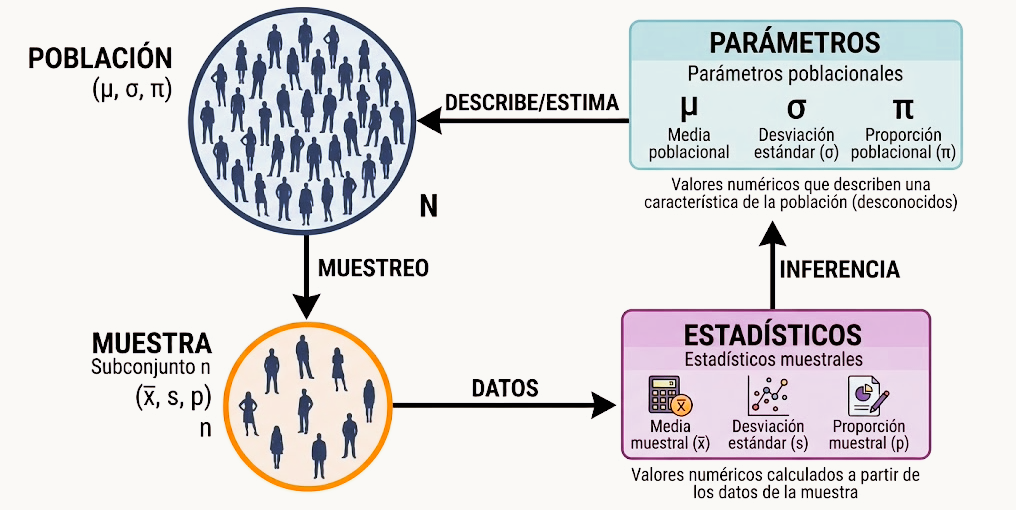
\includegraphics[width=0.75\linewidth,height=\textheight,keepaspectratio]{unidad_2/images/poblacion_muestra.png}
\end{center}

La \textbf{distribución muestral de un estadístico} es la distribución
de todos los valores posibles que ese estadístico puede tomar al
calcularse en muestras aleatorias del mismo tamaño extraídas de una
misma población. Este concepto es central en la inferencia estadística,
ya que permite cuantificar la incertidumbre asociada a las estimaciones.

Para comprender mejor qué es una distribución muestral y cómo se
construye, pueden ver la siguiente videoclase:

➡️ \href{https://youtu.be/UgWW88s5vYQ}{\textbf{Distribuciones
Muestrales}}

Como construir una distribución muestral puede resultar muy laborioso
cuando la población es grande, y directamente imposible si es infinita,
se suelen utilizar aproximaciones basadas en la toma de un gran número
de muestras aleatorias del mismo tamaño.

\section{Intervalos de Confianza (IC)}\label{intervalos-de-confianza-ic}

Una forma eficaz de abordar la inferencia estadística es a través de los
\textbf{intervalos de confianza (IC)}, ya que, aunque son procedimientos
inferenciales, están estrechamente vinculados con la estadística
descriptiva.

Supongamos que queremos estimar la \textbf{media de colesterol} de la
población de Mar del Plata. Sería inviable medir el colesterol de cada
habitante, por lo que optamos por tomar una muestra de, por ejemplo,
100, 200 o 300 individuos (más adelante veremos cómo determinar el
tamaño adecuado de la muestra). Debemos recordar que diferentes muestras
producirán en general medias diferentes. Existe, por tanto, un grado de
incertidumbre asociado. Si hiciéramos una estimación puntual,
obtendríamos un solo valor, pero sin información sobre su variabilidad.
No sabríamos qué tan cerca o lejos está nuestra estimación (\(\bar{x}\))
de la verdadera media poblacional (\(\mu\)).

El \textbf{intervalo de confianza} proporciona un rango de valores
dentro del cual se espera que se encuentre el valor verdadero del
parámetro poblacional, con un cierto nivel de confianza. A diferencia de
la estimación puntual que proporciona un único valor numérico, el
intervalo consta de dos valores entre los cuales se supone está
contenido el parámetro estimado. Entonces, el intervalo de confianza
puede expresarse como:

\[ 
IC = estimador~puntual \pm (coeficiente~de~confiabilidad) * (error~ estandar) 
\]

donde:

\begin{itemize}
\item
  \textbf{Estimador puntual}:

  \begin{itemize}
  \item
    Para la media poblacional (\(\mu\)), se toma la media
    muestral(\(\bar{x}\)).
  \item
    Para una proporción de la población (\(p\)), se toma la proporción
    muestral (\(\hat{p}\)).
  \end{itemize}
\item
  \textbf{Coeficiente de confiabilidad:} Se relaciona con el nivel de
  confianza deseado (por ejemplo, 90\%, 95\% o 99\%), y se expresa como
  \(1 - \alpha\), es decir la probabilidad de que el parámetro se
  encuentre dentro del IC. Recordemos que el nivel de significancia
  (\(\alpha\)) es la probabilidad de que el parámetro no se halle dentro
  del IC y es un valor generalmente pequeño (por ejemplo, 0.1, 0.05 o
  0.01) expresado como probabilidad o porcentaje (por ejemplo, 10\%, 5\%
  o 1\%).
\item
  \textbf{Error estándar (SE):} Representa la variabilidad de la
  distribución muestral. Por ejemplo, para la media el error estándar se
  calcula como la raíz cuadrada de la varianza de la distribución
  muestral:
\end{itemize}

\[ 
  SE = \frac{\sigma}{\sqrt{n}} 
\]

Donde \(\sigma\) es la desviación estándar poblacional y \(n\) el tamaño
de la muestra. Si se estima un IC para una proporción, el error estándar
es:

\[ 
  SE = \sqrt{\frac{\hat{p}(1 - \hat{p})}{n}} 
\]

El proceso se fundamenta en el Teorema del Límite Central (TCL), que
establece que, para muestras suficientemente grandes, la distribución de
\(\bar{x}\) es aproximadamente normal, con media \(\mu\) y varianza
\(\sigma^2/n\). Así, la variable tipificada:

\[ 
Z = \frac{\bar{x}-\mu}{\sigma} 
\]

sigue una distribución normal estándar (media 0 y desviación estándar
1), lo que permite calcular probabilidades y construir el IC.

En cualquier distribución normal:

\begin{itemize}
\item
  Entre \(\mu \pm \sigma\) se encuentra el 68\% de los datos.
\item
  Entre \(\mu \pm 2\sigma\) se encuentra el 95\%.
\item
  Entre \(\mu \pm 3\sigma\) se encuentra el 99\%.
\end{itemize}

El siguiente gráfico ilustra lo explicado anteriormente:

\begin{center}
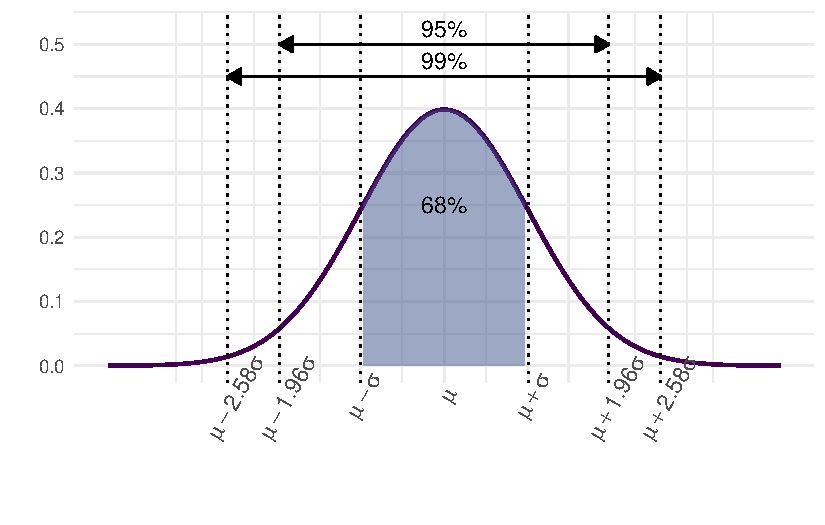
\includegraphics[width=0.85\linewidth,height=\textheight,keepaspectratio]{unidad_2/03_inferencia_files/figure-pdf/fig1-1.pdf}
\end{center}

Sabemos que, independientemente de la localización de los valores,
aproximadamente el \textbf{95\%} de los valores posibles de \(\bar{x}\)
en la distribución muestral estarán a menos de dos desviaciones estándar
de la media \(\mu\). Es decir, el intervalo \(\mu \pm 2\sigma\)
contendrá el \textbf{95\%} de los valores posibles de \(\bar{x}\).

Supongamos que formamos intervalos a partir de todos los posibles
valores de \(\bar{x}\), calculados a partir de todas las muestras
posibles de tamaño \(n\) tomadas de la población de interés. Esto
generará una gran cantidad de intervalos de la forma
\(\mu \pm  2\sigma\), todos con la misma amplitud, centrados en torno a
una \(\mu\) desconocida.

Aproximadamente el \textbf{95\%} de estos intervalos tendrán sus centros
dentro del intervalo \(\mu \pm  2\sigma\). Cada uno de estos intervalos,
que se encuentran dentro de \(\mu \pm  2\sigma\), puede contener el
valor verdadero de \(\mu\).

\begin{center}
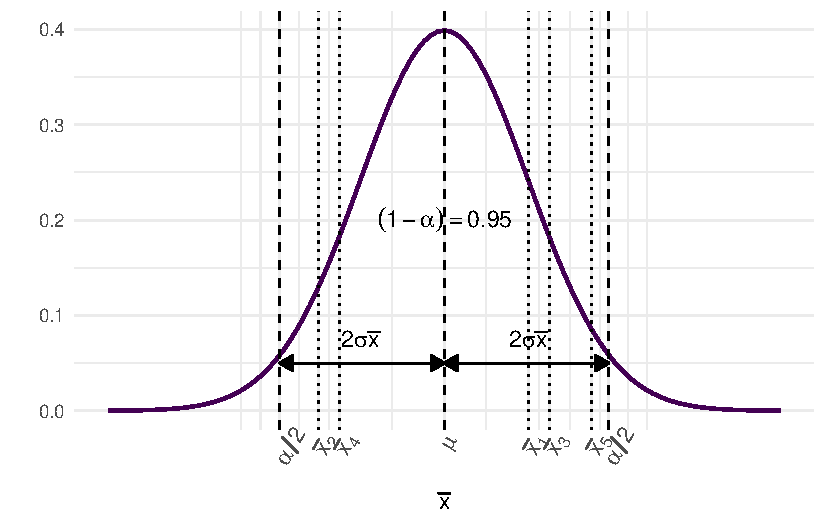
\includegraphics[width=0.85\linewidth,height=\textheight,keepaspectratio]{unidad_2/03_inferencia_files/figure-pdf/fig2-1.pdf}
\end{center}

Finalmente, y basándonos en las propiedades de la distribución Normal,
se puede deducir la expresión del IC:

\[ 
P(Z_{\alpha/2} < Z_{1-\alpha/2)} = 1 - \alpha 
\] Reemplazando \(Z\):

\[ 
P(Z_{\alpha/2} < \frac{\bar{x} - \mu}{\frac{\sigma}{\sqrt{n}}} < Z_{(1-\alpha/2)}) = 1-\alpha   
\]

Reordenando, la expresión del IC para la media queda:

\[ 
\bar{x} - Z_{\alpha/2}\sqrt{\frac{\sigma^2}{n}} < \mu < \bar{x} + Z_{\alpha/2}\frac{\sigma^2}{n}   
\]

\subsection{¿Cómo se interpreta un
IC?}\label{cuxf3mo-se-interpreta-un-ic}

Si hubiésemos tomado múltiples muestras del mismo tamaño de la
población, en al menos \(100 * (1 − \alpha)\%\) de las ocasiones el
intervalo calculado contendría el parámetro poblacional real. Es decir,
un IC al 95\% implica que, a largo plazo, el 95\% de los intervalos
obtenidos a partir de muestras repetidas incluirán el valor verdadero
del parámetro.

El producto del coeficiente de confiabilidad y el error estándar se
denomina \textbf{precisión de la estimación} y es el componente
responsable de la amplitud del IC. Recordemos que la fórmula general
para construir un intervalo de confianza era:

\[ 
IC = estimador~puntual \pm (coeficiente~de~confiabilidad) * (error~ estandar) 
\]

Para el caso de la media:

\begin{itemize}
\item
  \textbf{Aumento de la confiabilidad:} Si se incrementa el nivel de
  confianza, el coeficiente (por ejemplo, pasando de 1.96 a un valor
  mayor) aumenta, lo que a su vez incrementa la amplitud del IC.
\item
  \textbf{Reducción del error estándar:} Si se fija la confiabilidad
  (por ejemplo, al 95\%), para disminuir la amplitud del IC es necesario
  reducir el error estándar. Dado que el error estándar de la media es:
\end{itemize}

\[
   SE = \frac{\sigma}{\sqrt{n}} 
\]

y considerando que \(\sigma\) es constante, la única forma de disminuir
el error estándar es aumentando el tamaño muestral (\(n\)).

Surge entonces la pregunta: \textbf{¿qué tan grande debe ser} \(n\)?\\
La respuesta dependerá de \(\sigma\), del nivel de significación
(\(\alpha\)) y de la amplitud deseada para el IC. La relación es:

\[ 
Amplitud = Z \frac{\sigma}{\sqrt{n}} \Longrightarrow n = \frac{Z^2\sigma^2}{Amplitud^2} \quad (Z = 1.96~si~\alpha = 0.05) 
\]

(En la práctica, \(\sigma\) generalmente no se conoce, así que se usa su
estimación muestral).

La expresión del error estándar varía según el parámetro a estimar.
Hemos visto el caso de la media; si lo que se desea es calcular un IC
para una proporción, recordemos que, para muestras grandes, la
distribución de las proporciones de la muestra es aproximadamente normal
de acuerdo con el TCL. En este caso:

\begin{itemize}
\item
  La media de la distribución es la proporción real \(p\)
\item
  La varianza es \(p(1-p)/n\), lo que nos lleva a que el error estándar
  es:
\end{itemize}

\[ 
SE = \sqrt{\frac{\hat{p}(1-\hat{p})}{n}}      
\]

y el IC para la proporción se expresa como:

\[ 
\hat{p} - Z_{1-\alpha/2}\sqrt{\frac{\hat{p}(1-\hat{p})}{n}} < p < \hat{p} + Z_{1-\alpha/2}\sqrt{\frac{\hat{p}(1-\hat{p})}{n}}  
\]

Dado que un intervalo de confianza implica una declaración
probabilística, su cálculo se fundamenta en las distribuciones
muestrales de los estimadores y en el correspondiente error estándar.
Aunque las fórmulas pueden parecer complejas, los paquetes estadísticos
(como R) realizan estos cálculos automáticamente. Lo fundamental es
comprender en qué depende la amplitud del IC (nivel de confianza, error
estándar y tamaño muestral) y cómo cada uno de estos componentes influye
en la precisión de la estimación.

Para profundizar y visualizar simulaciones sobre estos conceptos, pueden
explorar recursos interactivos como:

➡️
\href{https://seeing-theory.brown.edu/frequentist-inference/es.html\#section2}{\textbf{Viendo
la teoría: Una introducción visual a probabilidad y estadística}}

Además, existe un ejemplo práctico de cálculo de IC para la media
utilizando la distribución \(t\) de Student en el siguiente enlace:

➡️
\href{https://cballejo.github.io/R_Epi_Avanzada/Unidad2/IC/}{\textbf{Intervalos
de confianza con R}}

\section{Test de hipótesis}\label{test-de-hipuxf3tesis}

Aunque los estudios de corte transversal no se diseñan originalmente con
grupos de comparación, en aquellos de carácter más analítico es
frecuente establecer comparaciones. Por ejemplo, pueden surgir preguntas
como:

\emph{¿La prevalencia de la enfermedad es mayor en mujeres, en
determinados grupos etarios o en una provincia específica?}

Con esto en mente, revisaremos las herramientas que permiten comparar
grupos mediante test o contrastes de hipótesis. El propósito de estos
test es ofrecer al investigador una herramienta para tomar decisiones
sobre la población a partir de la información obtenida en una muestra.

Antes de adentrarnos en la parte estadística, es importante distinguir
entre dos tipos de hipótesis:

\begin{itemize}
\item
  \textbf{Hipótesis de investigación:} Es la conjetura o suposición que
  motiva la investigación.
\item
  \textbf{Hipótesis estadística:} Es aquella que puede ser evaluada
  mediante técnicas estadísticas apropiadas.
\end{itemize}

En este texto nos centraremos en aclarar aspectos relativos a las
hipótesis estadísticas, asumiendo que las hipótesis de investigación ya
han sido discutidas previamente por los investigadores. Describiremos
brevemente el razonamiento subyacente a estos test.

Los contrastes de hipótesis parten de una \textbf{hipótesis nula}, la
cual afirma que los dos grupos comparados son iguales o, en otras
palabras, que las diferencias observadas se deben únicamente al azar.
Como ya se ha mencionado, la variabilidad intrínseca de cualquier
muestra impide que la diferencia entre grupos sea exactamente cero.

El método estadístico nos permite cuantificar la diferencia entre grupos
asumiendo que, si repitiésemos el experimento infinitas veces obtenemos
todas las posibles muestras del tamaño indicado a partir de nuestras
poblaciones (\emph{distribución muestral}), las diferencias entre grupos
``iguales'' se distribuirían conforme a una curva teórica. Basándonos en
las propiedades de esta distribución, podemos determinar un valor límite
que comprende, por ejemplo, el 95\% o el 99\% de las diferencias
esperadas. Si la diferencia observada entre las muestras supera este
valor límite, se considera excesiva para ser atribuible al azar y, por
tanto, se rechaza la hipótesis nula. Por el contrario, si la diferencia
cae dentro del área del 95\%, se concluye que la diferencia encontrada
podría atribuirse al azar, y no habría evidencia que nos permita
rechazar la hipótesis nula. En estos casos decimos que los grupos ``no
son diferentes'' pero no ``son iguales'', ya que la variabilidad
inherente impide probar una igualdad exacta.

Los contrastes de hipótesis se realizan generalmente bajo las siguientes
condiciones:

\begin{itemize}
\item
  Se asume a priori que la ley de distribución de la población es
  conocida.
\item
  Se extrae una muestra aleatoria de dicha población.
\end{itemize}

El conjunto de estas técnicas de inferencia se denomina \textbf{técnicas
paramétricas}. Sin embargo, existen otros métodos, denominados
\textbf{técnicas no paramétricas} o contrastes de distribuciones libres,
que no requieren estimar parámetros ni suponer una ley de probabilidad
específica para la población. Algunos de estos métodos serán
desarrollados más adelante en este módulo.

Es importante señalar que los contrastes de hipótesis se utilizan no
solo en estudios transversales, sino con mayor frecuencia en diseños en
los que \emph{a priori} existen grupos de comparación, como en estudios
de casos y controles, cohortes, ensayos clínicos, entre otros.
Desarrollaremos aquí la teoría que los sustenta y los utilizaremos a lo
largo de todo el curso.

\subsection{Estructura del test de
hipótesis}\label{estructura-del-test-de-hipuxf3tesis}

Los componentes básicos de cualquier test de contraste de hipótesis son:

\begin{itemize}
\item
  \textbf{Hipótesis nula} (\(H_0\)): Afirma que no existe diferencia
  entre los grupos que se comparan, es decir, que las variaciones
  observadas se deben únicamente al azar.
\item
  \textbf{Hipótesis alternativa} (\(H_1\)): Es la conjetura o suposición
  que plantea el investigador, estableciendo que sí existe una
  diferencia entre los grupos. Generalmente es complementaria de la
  \(H_0\).
\item
  \textbf{Estadístico de prueba}: Es el valor calculado a partir de los
  datos muestrales que se utiliza para tomar la decisión sobre la
  \(H_0\). Cada tipo de problema tiene un estadístico adecuado, cuya
  magnitud, al compararse con su distribución muestral (por ejemplo, la
  distribución normal estándar en el caso del estadístico \(Z\)),
  permite determinar si las diferencias observadas son atribuibles al
  azar.
\item
  \textbf{Valor crítico o Región crítica}: La región crítica se
  establece en función del nivel de significación (\(\alpha\)) y
  consiste en el conjunto de valores extremos del estadístico de prueba
  que, de ser alcanzados, llevarían a rechazar la \(H_0\). Todos los
  posibles valores del estadístico se ubican en el eje horizontal de la
  gráfica de su distribución, y la región crítica delimita aquellos
  valores que son muy poco probables bajo la hipótesis nula.
\end{itemize}

\begin{center}
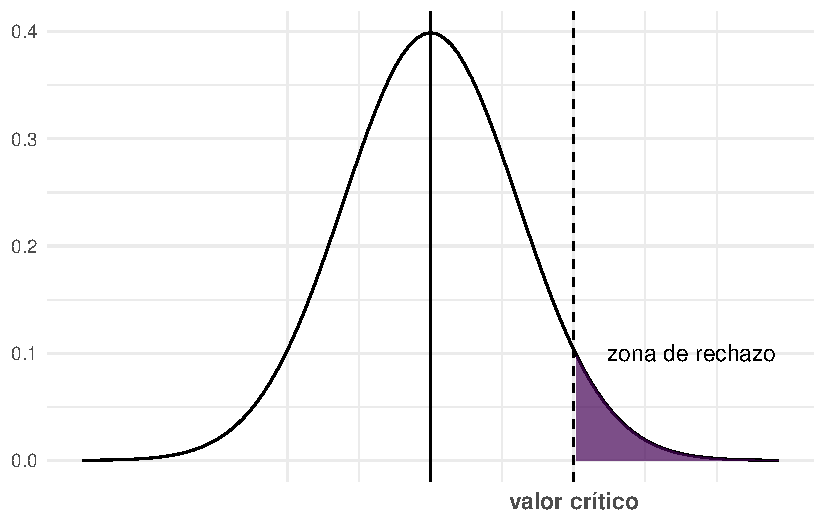
\includegraphics[width=0.85\linewidth,height=\textheight,keepaspectratio]{unidad_2/03_inferencia_files/figure-pdf/fig3-1.pdf}
\end{center}

La regla de decisión es la siguiente:

\begin{itemize}
\item
  Si el valor del estadístico de prueba calculado a partir de la muestra
  cae en la región crítica, se rechaza la \(H_0\)\hspace{0pt} y se
  concluye que las diferencias observadas son \textbf{estadísticamente
  significativas}.
\item
  Si el valor no cae en la región crítica, no se rechaza la
  \(H_0\)\hspace{0pt}; esto indica que las diferencias entre lo
  observado y lo esperado pueden explicarse por el azar. Es decir,
  \textbf{no son estadísticamente significativas}.
\item
  \textbf{Nivel de significación} (\(\alpha\)): Es la probabilidad de
  cometer un error tipo I, es decir, rechazar \(H_0\) cuando es
  verdadera. Este valor, elegido por el investigador (comúnmente 5\% o
  1\%), determina el límite entre la región de no rechazo y la región
  crítica.
\item
  \textbf{Valor \emph{p}}: Es una medida de qué tan probable son los
  resultados de la muestra, considerando que \(H_0\) sea verdadera.

  \begin{itemize}
  \item
    Un valor \(p\) muy pequeño indica que es muy poco probable obtener
    los resultados observados para el estadístico muestral si \(H_0\)
    fuese cierta, por lo que debemos rechazarla.
  \item
    Esto significa que si el valor \(p \leq \alpha\), es posible
    rechazar \(H_0\); mientras que si \(p > \alpha\), no es posible
    rechazar la hipótesis nula.
  \end{itemize}

  Por ejemplo, si en un test de contraste de dos proporciones se obtiene
  un estadístico \(Z= 3,034\) y un valor \(p = 0.0024\), esto significa
  que la probabilidad de obtener un valor de \(Z\) de 3.034 o mayor,
  suponiendo que \(H_0\) es cierta, es del 0.24\%. Dado que este valor
  es mucho menor que un nivel de significación del 5\% (o incluso del
  1\%), se rechaza \(H_0\) y se concluye que la diferencia observada es
  estadísticamente significativa. En otras palabras, si bajo un supuesto
  dado, la probabilidad de un suceso observado particular es
  excepcionalmente pequeña, concluimos que el supuesto probablemente es
  incorrecto (\emph{regla del suceso infrecuente}).
\end{itemize}

\subsection{Tipos de contrastes}\label{tipos-de-contrastes}

Los contrastes de hipótesis se clasifican según la forma de la hipótesis
alternativa (\(H_1\)). Esta clasificación determina si la prueba es
\textbf{unilateral} (de cola izquierda o derecha) o \textbf{bilateral}
(de dos colas). Siendo las colas de la distribución las regiones
extremas limitadas por los valores críticos.

\subsubsection{Test de cola izquierda}\label{test-de-cola-izquierda}

La hipótesis alternativa plantea que la media del primer grupo es
significativamente \textbf{menor} que la del segundo:

\[
H_1: \mu_1 < \mu_2
\]

La región crítica se encuentra en el extremo izquierdo de la
distribución. Todo el área crítica tiene un tamaño \(\alpha\) con un
valor crítico de \(-1,645\).

\begin{center}
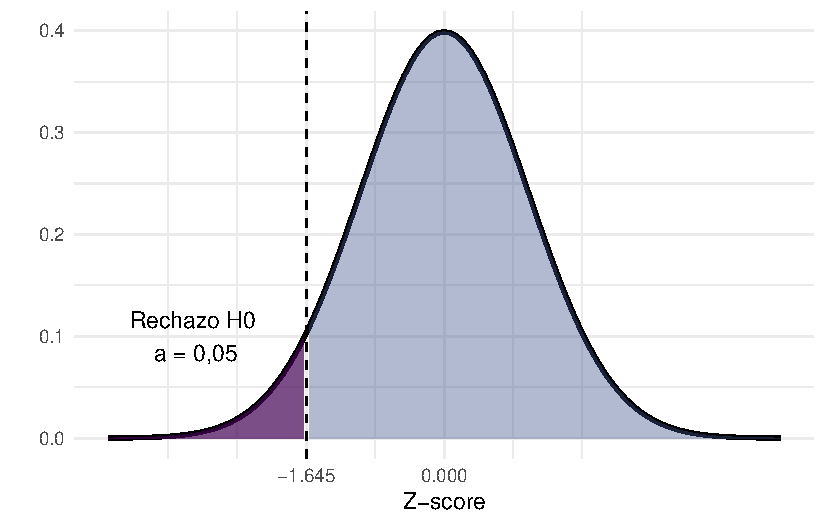
\includegraphics[width=0.85\linewidth,height=\textheight,keepaspectratio]{unidad_2/03_inferencia_files/figure-pdf/fig4-1.pdf}
\end{center}

\subsubsection{Test de cola derecha}\label{test-de-cola-derecha}

La hipótesis alternativa establece que la media del primer grupo es
significativamente \textbf{mayor} que la del segundo:

\[ 
H_1: \mu_1 > \mu_2 
\]

La región crítica se concentra en el extremo derecho de la distribución
y toda el área crítica tiene un tamaño \(\alpha\) con un valor crítico
de \(1,645\).

\begin{center}
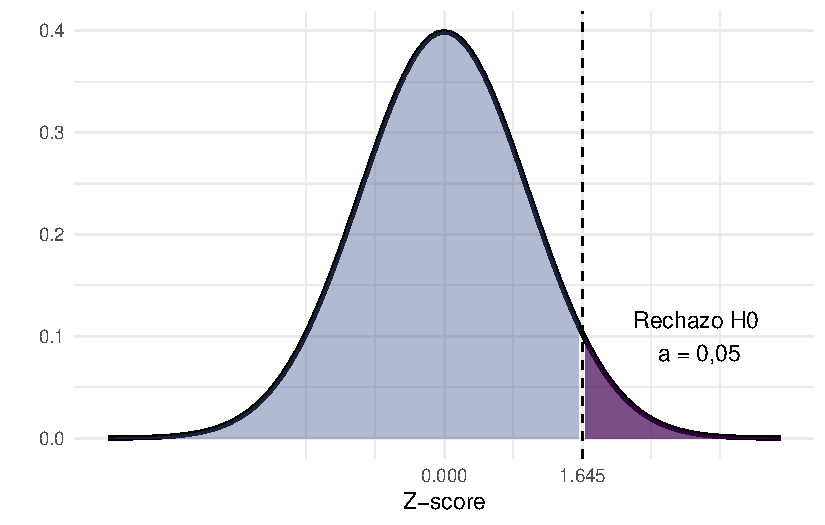
\includegraphics[width=0.85\linewidth,height=\textheight,keepaspectratio]{unidad_2/03_inferencia_files/figure-pdf/fig5-1.pdf}
\end{center}

\subsubsection{Pruebas bilaterales}\label{pruebas-bilaterales}

La hipótesis alternativa afirma que existen diferencias entre los
grupos, \textbf{sin especificar la dirección}:

\[
H_1: \mu_1 \neq \mu_2
\]

La región crítica se divide entre ambos extremos de la distribución, con
valores críticos de \(\pm 1,96\). El nivel de significación total
(\(\alpha\)) se reparte en partes iguales entre las dos colas
(\(\alpha/2\) en cada una), lo que implica un 2,5\% de probabilidad en
cada cola si \(H_0\) es verdadera.

\begin{center}
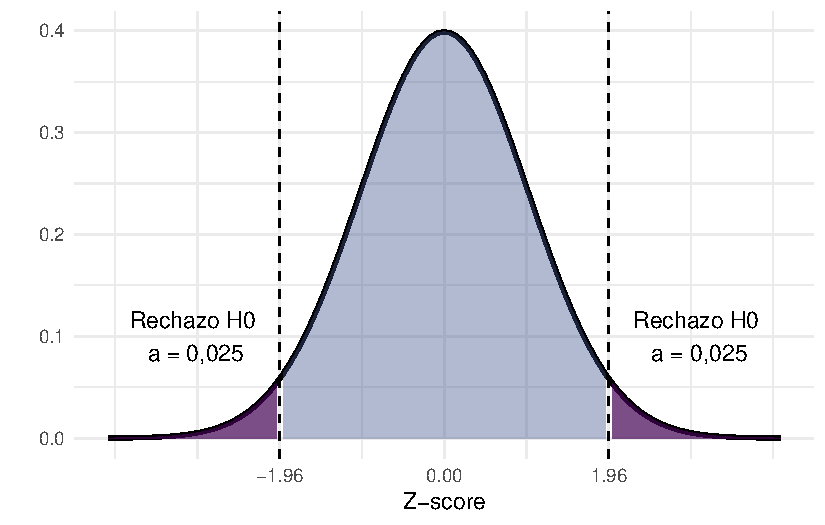
\includegraphics[width=0.85\linewidth,height=\textheight,keepaspectratio]{unidad_2/03_inferencia_files/figure-pdf/fig6-1.pdf}
\end{center}

\subsection{Errores}\label{errores}

Al utilizar el razonamiento de los contrastes de hipótesis, existen dos
tipos principales de errores que podemos cometer:

\begin{itemize}
\item
  \textbf{Error tipo I} (\(\alpha\)): Ocurre cuando el investigador
  rechaza la hipótesis nula (\(H_0\)) siendo esta verdadera en la
  población y se concluye erróneamente que existe una diferencia cuando
  en realidad no la hay. Se suele eligir un valor pequeño de \(\alpha\)
  (0.01, 0.05 y 0.10) para hacer que la probabilidad de rechazo de
  \(H_0\) sea pequeña.
\item
  \textbf{Error tipo II (}\(\beta\)): Ocurre cuando el investigador no
  rechaza la \(H_0\) siendo esta falsa en la población, es decir, se
  falla en detectar una diferencia real. Generalmente \(\beta\) es mayor
  que \(\alpha\), pero su valor real se desconoce en la práctica.
\end{itemize}

Es importante notar que, una vez que se realiza el procedimiento de
prueba, no es posible saber con certeza si se ha cometido alguno de
estos errores, ya que se desconoce el verdadero estado de la realidad.
Sin embargo, al fijar un \(\alpha\) pequeño, se busca asegurar que, en
caso de rechazar la \(H_0\), la probabilidad de haber cometido un error
Tipo I sea baja.

En resumen, al interpretar los resultados de un test de hipótesis:

\begin{itemize}
\item
  \textbf{Si se rechaza la} \(H_0\): se asume que la probabilidad de
  haber cometido un error Tipo I es baja (debido al valor pequeño de
  \(\alpha\)).
\item
  \textbf{Si no se rechaza la} \(H_0\): se desconoce el riesgo real de
  un error Tipo II, pero es importante tener en cuenta que, en muchas
  situaciones, este riesgo es mayor que el de un error Tipo I.
\end{itemize}

La tabla que se presenta a continuación resume las posibles situaciones
a las que nos enfrentamos con los test de hipótesis:

{\def\LTcaptype{none} % do not increment counter
\begin{longtable}[]{@{}lll@{}}
\toprule\noalign{}
& No rechazar H0 & Rechazar H0 \\
\midrule\noalign{}
\endhead
\bottomrule\noalign{}
\endlastfoot
H0 es cierta & Correcto (1-α) & Error tipo I (α) \\
H0 es falsa & Error tipo II (β) & Correcto (1-β) \\
\end{longtable}
}

Para quienes están familiarizados con el ámbito del diagnóstico, existe
una clara analogía entre los falsos positivos y falsos negativos en las
pruebas diagnósticas y, respectivamente, el error Tipo I y el error Tipo
II en los contrastes de hipótesis.

Hemos discutido el significado de \(\alpha\) (error Tipo I); ahora
veamos qué implica \(\beta\). Recordemos que el error Tipo II es análogo
a los falsos negativos de las pruebas diagnósticas: es la probabilidad
de no detectar una diferencia cuando, en realidad, ésta existe. En otras
palabras, \(\beta\) es la probabilidad de no rechazar la hipótesis nula
(\(H_0\)\hspace{0pt}) siendo esta falsa.

A diferencia de \(\alpha\) que se fija en un único valor y es
determinado por el investigador, \(\beta\) varía según el valor real del
parámetro en estudio. Por ejemplo, si consideramos la hipótesis nula
\(H_0: \mu_1 - \mu_2 = 0\), habrá un valor de \(\beta\) para cada
posible diferencia entre \(\mu_1\)\hspace{0pt} y \(\mu_2\) cuando el
valor real no sea cero. La probabilidad de detectar correctamente una
diferencia real - es decir, de obtener un resultado estadísticamente
significativo cuando la diferencia existe- se denomina \textbf{potencia
estadística} y se expresa como \(1-\beta\).

Los contrastes de hipótesis no son exclusivos de los estudios
transversales; por el contrario, su uso es más común en estudios
analíticos que involucran grupos de comparación, tales como estudios de
casos y controles, cohortes o ensayos clínicos. Por ejemplo, en un
ensayo clínico que evalúa dos tratamientos, la potencia estadística
refleja la capacidad del estudio para identificar un efecto real del
tratamiento.

Es deseable que la potencia del estudio sea lo mayor posible, ya que
esto incrementa la probabilidad de detectar diferencias verdaderas. Sin
embargo, no es posible minimizar ambos errores simultáneamente ya que al
disminuir \(\alpha\) (es decir, al ser más exigentes para rechazar la
\(H_0\)\hspace{0pt}), \(\beta\) tiende a aumentar, y viceversa. En los
contrastes, la hipótesis privilegiada es \(H_0\) que solo será rechazada
cuando la evidencia de su falsedad supere el umbral del \(1-\alpha\).
Esto significa que, a menos que la evidencia en contra de \(H_0\) sea
muy significativa, se opta por no rechazarla. Lo ideal a la hora de
definir un test es encontrar un compromiso entre \(\beta\) y \(\alpha\).

\begin{center}
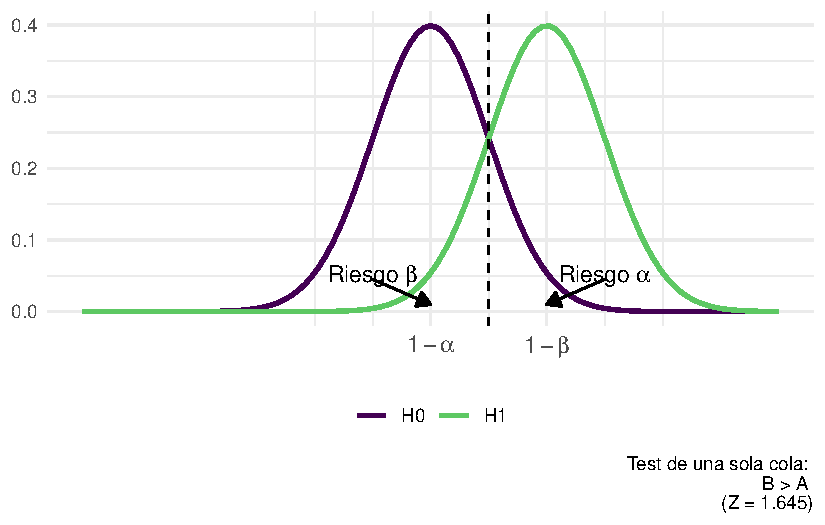
\includegraphics[width=0.85\linewidth,height=\textheight,keepaspectratio]{unidad_2/03_inferencia_files/figure-pdf/fig7-1.pdf}
\end{center}

Mientras que para tests bilaterales:

\begin{center}
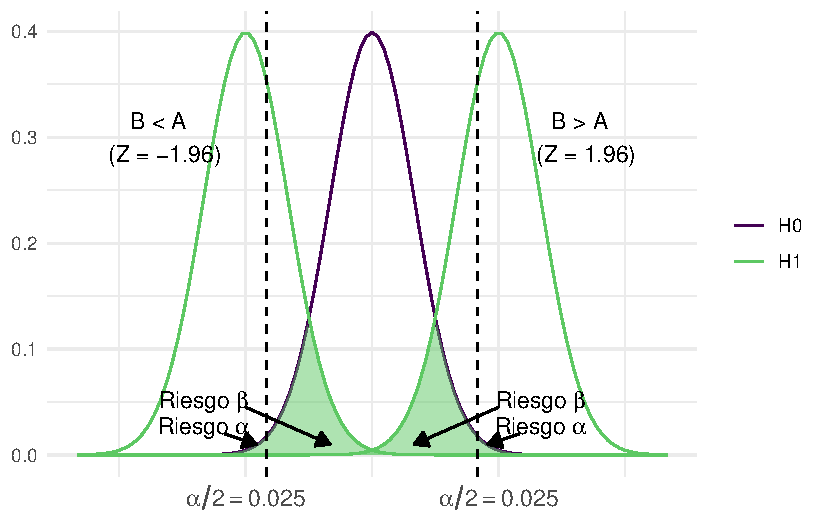
\includegraphics[width=0.85\linewidth,height=\textheight,keepaspectratio]{unidad_2/03_inferencia_files/figure-pdf/fig8-1.pdf}
\end{center}

Finalmente, podemos decir que la potencia estadística ofrece un segundo
mecanismo de seguridad en un contraste de hipótesis. Es como contar con
una protección adicional en la toma de decisiones: si solo dispusiéramos
del nivel de significación (\(\alpha\)), tendríamos menos garantías. Al
incorporar la potencia (\(1-\beta\)) agregamos un segundo control. Por
ello, en un contraste no basta con tener un valor \emph{p} pequeño;
también se necesita una potencia alta, que en la práctica suele fijarse
en un 80\% (es decir, \(1 - \beta = 0.8\)).\\
Por otro lado, cuando existe una diferencia real ---o un efecto real de
una terapia, o una verdadera diferencia entre dos fármacos---, la
\textbf{magnitud} de ese efecto influye en la facilidad para detectarlo.
Los efectos grandes son más fáciles de identificar que los pequeños.
Para estimar la potencia de una prueba, debemos especificar el
\textbf{efecto mínimo} que valga la pena identificar.

La potencia de un test estadístico depende de tres factores que actúan
de manera interrelacionada:

\begin{itemize}
\item
  El \textbf{riesgo de error} que se tolerará al rechazar la hipótesis
  de ausencia de efecto o diferencia (\(\alpha\)).
\item
  La \textbf{dimensión de la diferencia} que se desea identificar en
  relación con la variabilidad en las poblaciones.
\item
  El \textbf{tamaño de la muestra}.
\end{itemize}

Del mismo modo que en un problema de estimación se necesita una idea de
la magnitud a estimar y del error aceptable para definir el tamaño de la
muestra, en un contraste de hipótesis se requiere conocer el
\textbf{tamaño del efecto} que se quiere detectar. Así, el tamaño
muestral se determina en función del nivel de confianza y de la potencia
de la prueba, además de otros aspectos relacionados con el diseño y la
prueba estadística elegida.

En epidemiología, una de las situaciones más frecuentes al diseñar un
estudio es el cálculo del tamaño muestral para un \textbf{nivel de
confianza del 95\%} y una \textbf{potencia del 80\%}, que, como se
mencionó, es un nivel de potencia alto y que además permite manejar un
\(\alpha\) relativamente bajo. El lenguaje \textbf{R} cuenta con
diversas funciones para \textbf{calcular y visualizar} la relación entre
tamaño muestral, potencia, tamaño del efecto y nivel de confianza,
facilitando el diseño de estudios con un adecuado balance entre la
probabilidad de detectar diferencias reales y la de controlar errores
estadísticos.

Por ejemplo, la función \texttt{pwr.t.test()} del paquete \texttt{pwr}
(Champely 2020), calcula la potencia para pruebas \(t\) de Student de
medias (para una muestra, dos muestras y muestras pareadas), basado en
el tamaño de la muestra, el nivel de confianza y el tamaño de efecto:

\begin{Shaded}
\begin{Highlighting}[]
\FunctionTok{pwr.t.test}\NormalTok{(n, d, }\AttributeTok{sig.level =} \FloatTok{0.05}\NormalTok{, power, type, alternative)}
\end{Highlighting}
\end{Shaded}

Donde:

\begin{itemize}
\item
  \texttt{n}: Número de observaciones para cada grupo.
\item
  \texttt{d}: tamaño de efecto (\(d\) de Cohen) - diferencia
  (estandarizada) entre grupos.

  \begin{quote}
  \emph{Nota:} La \(d\) de Cohen representa las desviaciones estándar
  que separan dos o más grupos. Por ejemplo: \(d_{Cohen} = 0.5\)
  representa que la diferencia entre grupo experimental y muestral es de
  media desviación estándar. Cohen sugirió (provisoriamente) que 0.2 es
  un tamaño de efecto pequeño, 0.5 es mediano y 0.8 es grande,
  \end{quote}
\item
  \texttt{sig.level}: nivel de significación (probabilidad del error de
  tipo I).
\item
  \texttt{power}: potencia del test (1 menos la probabilidad del error
  tipo II).
\item
  \texttt{type}: tipo de test (\texttt{"two.sample"},
  \texttt{"one.sample"}, \texttt{"paired"}).
\item
  \texttt{alternative}: palabra que especifica la hipotesis alternativa,
  debe ser \texttt{"two.sided"} (predeterminado), \texttt{"greater"} or
  \texttt{"less"}.
\end{itemize}

La función se ejecuta incorporando todos los argumentos obligatorios
(\texttt{d},\texttt{n}, \texttt{power} y \texttt{sig.level}) menos el
que se quiere calcular. En ese caso se iguala a \texttt{NULL} o se
omite.

Supongamos que queremos conocer el tamaño de la muestra para detectar
diferencias en la media de la hemoglobina glicosilada entre dos grupos
de pacientes con tratamientos de control de la diabetes distintos.
Aceptamos un nivel de efecto convencional de una pequeña desviación
(\(d_{Cohen} = 0.2\)), una potencia del 80\% y una significación
habitual de 0,05.

Cargamos el paquete requerido:

\begin{Shaded}
\begin{Highlighting}[]
\FunctionTok{library}\NormalTok{(pwr)}
\end{Highlighting}
\end{Shaded}

Calculamos el tamaño de muestra:

\begin{Shaded}
\begin{Highlighting}[]
\FunctionTok{pwr.t.test}\NormalTok{(}
  \AttributeTok{d =} \FloatTok{0.2}\NormalTok{,}
  \AttributeTok{power =} \FloatTok{0.8}\NormalTok{,}
  \AttributeTok{sig.level =} \FloatTok{0.05}\NormalTok{,}
  \AttributeTok{type =} \StringTok{"two.sample"}\NormalTok{,}
  \AttributeTok{alternative =} \StringTok{"two.sided"}
\NormalTok{)}
\end{Highlighting}
\end{Shaded}

\begin{verbatim}

     Two-sample t test power calculation 

              n = 393.4057
              d = 0.2
      sig.level = 0.05
          power = 0.8
    alternative = two.sided

NOTE: n is number in *each* group
\end{verbatim}

También podemos graficar la salida:

\begin{Shaded}
\begin{Highlighting}[]
\FunctionTok{pwr.t.test}\NormalTok{(}
  \AttributeTok{d =} \FloatTok{0.2}\NormalTok{,}
  \AttributeTok{power =} \FloatTok{0.8}\NormalTok{,}
  \AttributeTok{sig.level =} \FloatTok{0.05}\NormalTok{,}
  \AttributeTok{type =} \StringTok{"two.sample"}\NormalTok{,}
  \AttributeTok{alternative =} \StringTok{"two.sided"}
\NormalTok{) }\SpecialCharTok{|\textgreater{}}
  \FunctionTok{plot}\NormalTok{()}
\end{Highlighting}
\end{Shaded}

\begin{center}
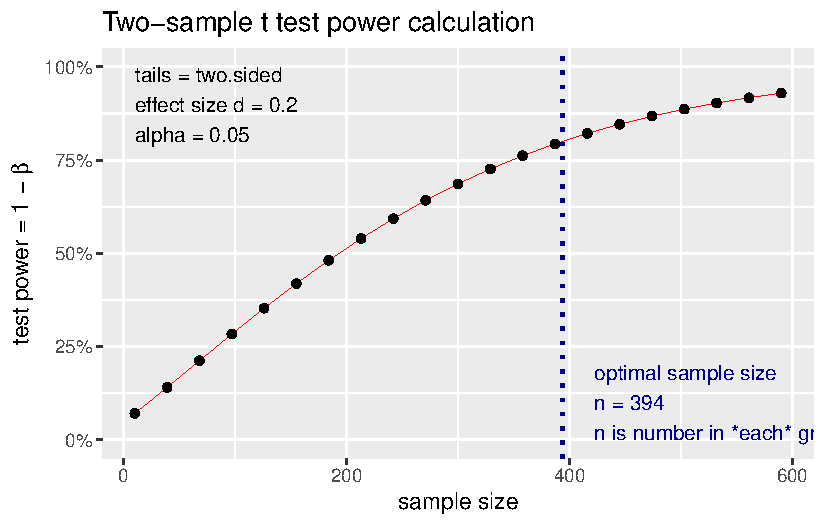
\includegraphics[width=0.85\linewidth,height=\textheight,keepaspectratio]{unidad_2/03_inferencia_files/figure-pdf/cod4-1.pdf}
\end{center}

Observamos que, si por ejemplo tomásemos una muestra de 300 individuos
por grupo, la potencia del estudio con ese tamaño de efecto y nivel de
significación del 0,05 sería aproximadamente de 68\%.

\subsection{¿Qué test se debe aplicar en cada
caso?}\label{quuxe9-test-se-debe-aplicar-en-cada-caso}

Hemos discutido la mecánica general de los test de hipótesis. Ahora, nos
centraremos en orientarnos sobre qué test aplicar en cada situación.
Aunque existe un desarrollo teórico detrás de cada caso, aquí nos
quedaremos con ciertas reglas prácticas.

Para sistematizar los contrastes de hipótesis, es útil responder dos
preguntas fundamentales:

\begin{itemize}
\item
  \textbf{¿Qué tipo de variable dependiente tengo?}\\
  La variable resultado puede ser cuantitativa, cualitativa, de tiempo
  hasta un evento, etc.
\item
  \textbf{¿Qué se está comparando?}\\
  Esto se traduce en evaluar el tipo de experimento: ¿se comparan dos
  grupos o más? ¿Son muestras independientes o relacionadas (por
  ejemplo, medidas en el mismo grupo antes y después de una
  intervención)?
\end{itemize}

\subsubsection{Variable resultado
cuantitativa}\label{variable-resultado-cuantitativa}

Cuando la variable de interés es cuantitativa, la comparación de grupos
generalmente se traduce en comparar las medias de dichos grupos. En este
contexto, se deben responder una tercera pregunta y es si dicha variable
se \emph{distribuye normalmente}, porque si no fuera así, debemos
recurrir a los contrastes \emph{no paramétricos}.

\begin{quote}
En la \href{04_norm_het.qmd}{\textbf{siguiente sección}} detallaremos
las pruebas de normalidad y heterogeneidad de varianzas y su aplicación
en R.
\end{quote}

Por ejemplo, para comparar dos grupos se plantearía:

\begin{itemize}
\tightlist
\item
  \(H_0: \mu_1 = \mu_2\) (o su equivalente \(\mu_1 - \mu_2 = 0\))
\item
  \(H_1: \mu_1 \neq \mu_2\) (contraste bilateral) o bien
  \(\mu_1 < \mu_2\) o \(\mu_1 > \mu_2\) (contrastes unilaterales).
\end{itemize}

Se calcula el estadístico de prueba (por ejemplo, \(t\) de Student o
\(Z\), según el tamaño de la muestra y si se conoce la varianza
poblacional), se determina la región de rechazo y, finalmente, si
\(p < \alpha\) rechazo \(H_0\) y si \(p >  \alpha\) no rechazo \(H_0\).

A continuación presentamos un esquema que sirve de guía para potenciales
situaciones:

\protect\phantomsection\label{fig9}
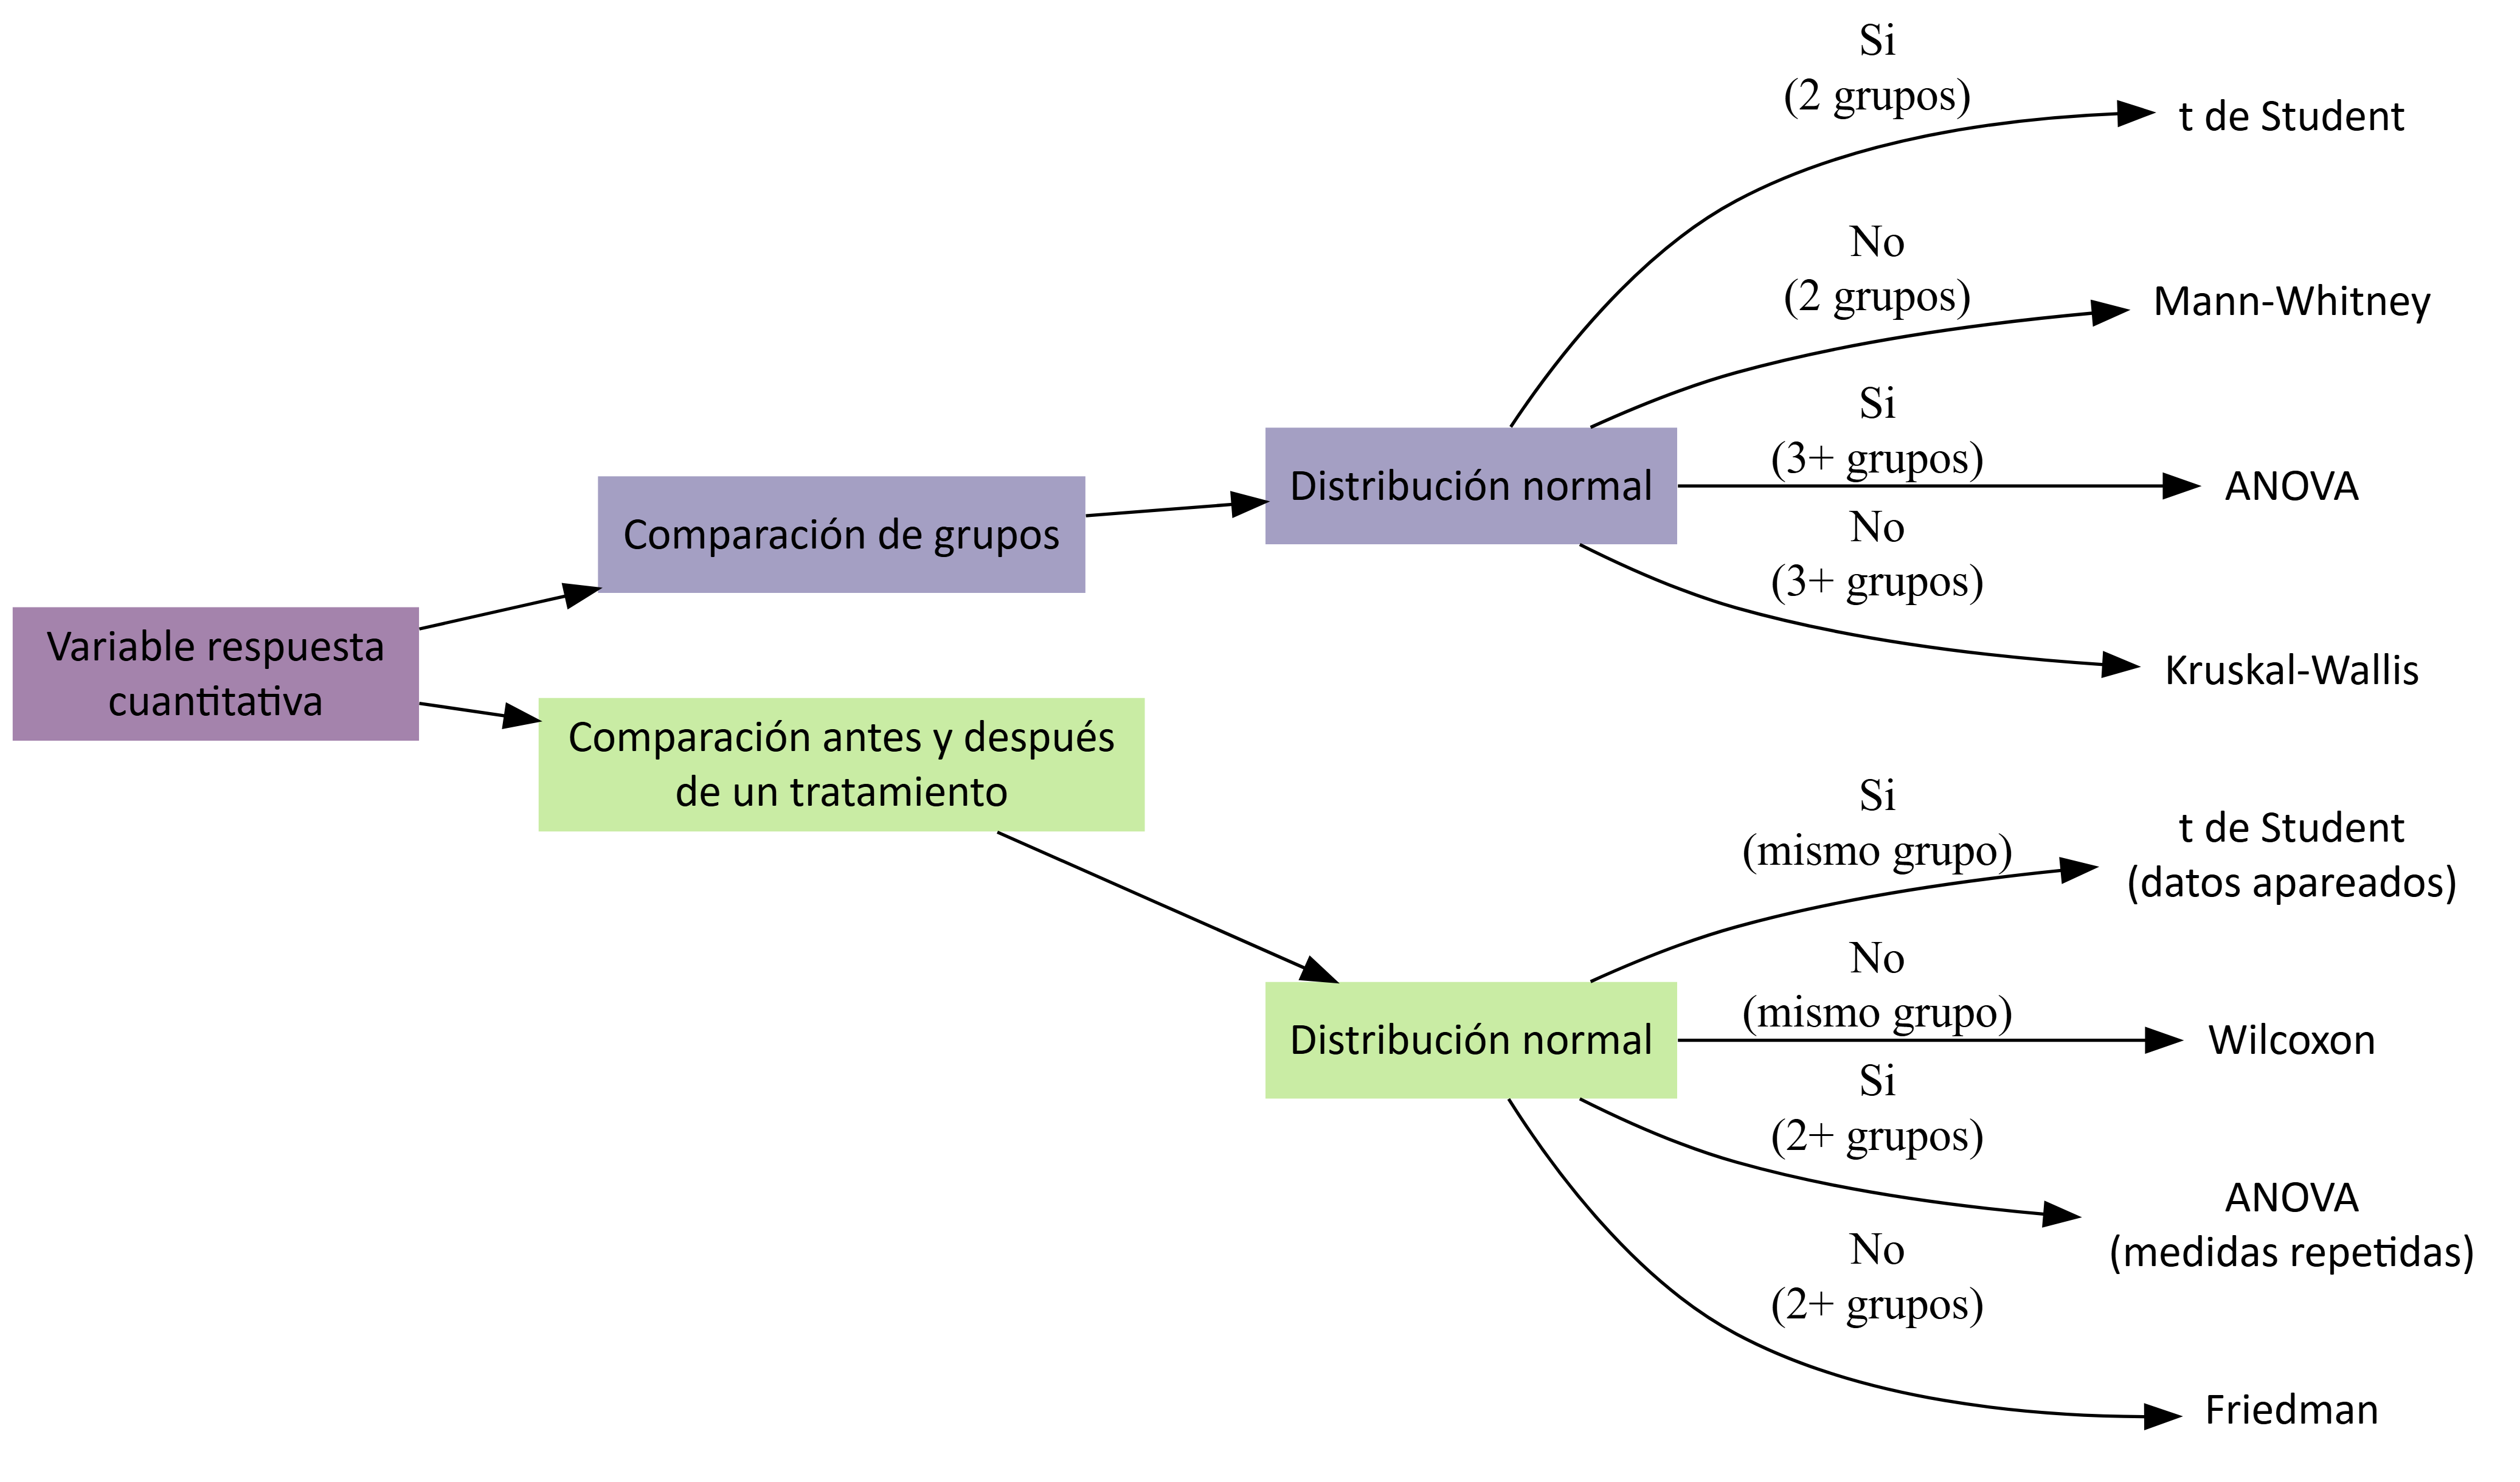
\includegraphics[width=5.5in,height=3.5in]{unidad_2/03_inferencia_files/figure-latex/dot-figure-4.png}

Hay algo más que los estadísticos nos ``obligan'' a considerar en el
caso que compare medias independientes y se haya verificado la
normalidad de la distribución, y se trata de considerar si las varianzas
de las poblaciones que comparo son iguales o diferentes. El algoritmo de
resolución es el siguiente:

\protect\phantomsection\label{fig10}
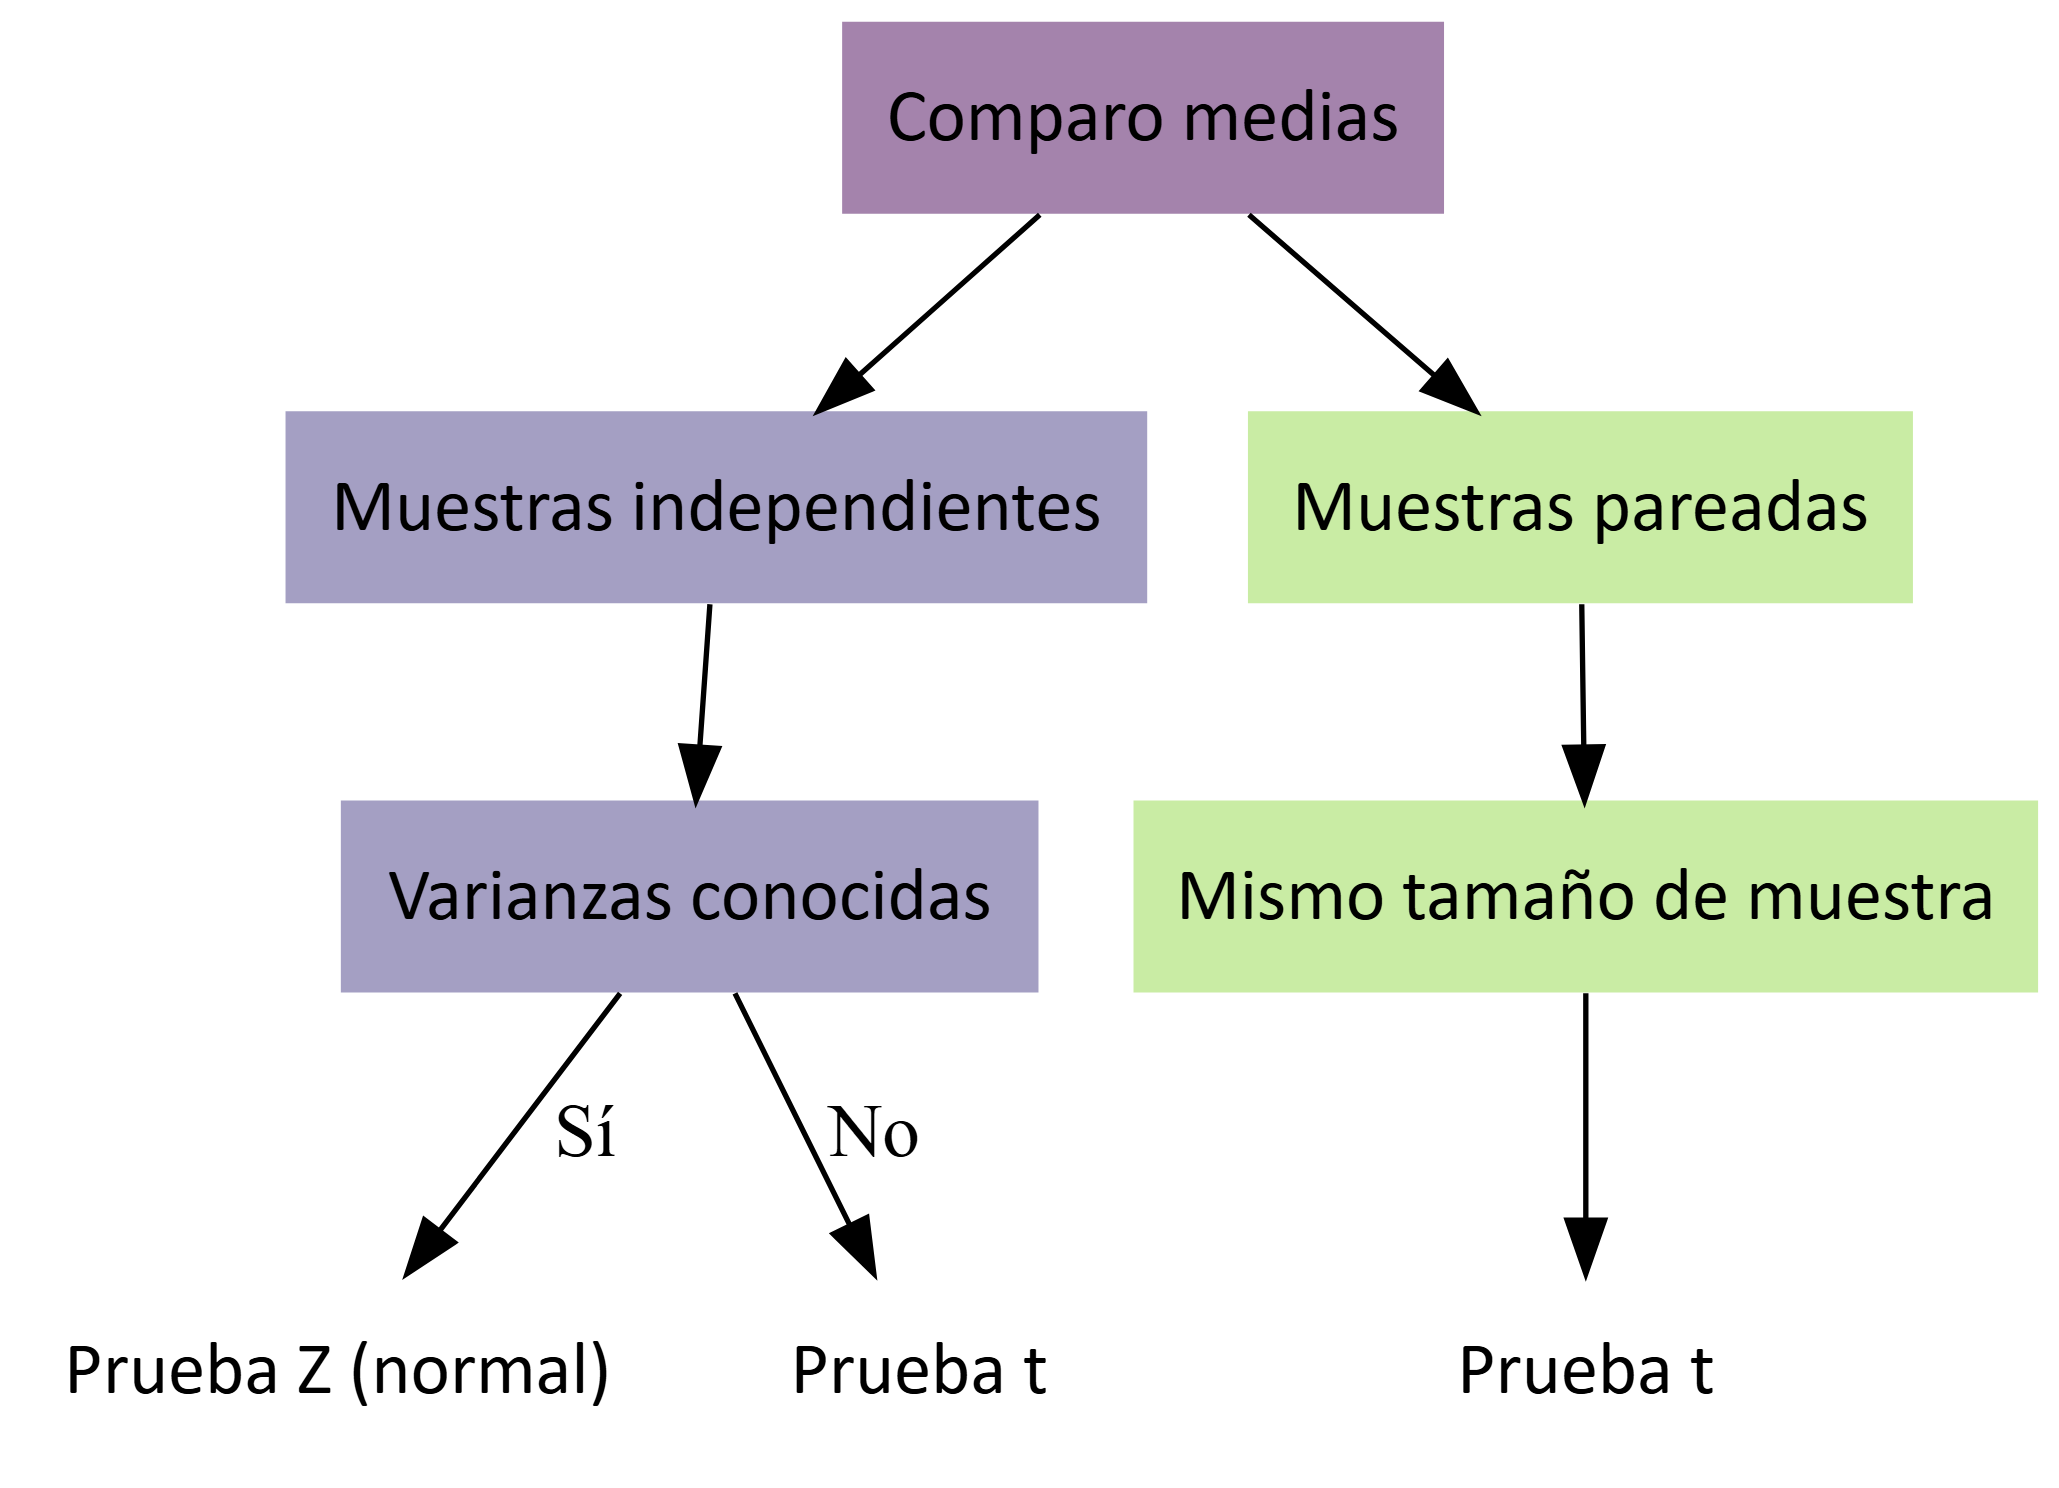
\includegraphics[width=5.5in,height=3.5in]{unidad_2/03_inferencia_files/figure-latex/dot-figure-6.png}

Cuando trabajamos con muestras independientes, a menudo nos encontramos
en el escenario de \emph{varianzas desconocidas}. Esto nos obliga a
realizar, de manera previa, un test de homogeneidad de varianzas para
determinar si se puede asumir que son iguales o si, por el contrario,
difieren. La razón es que, aunque se utiliza el estadístico \(t\) de
Student para comparar las medias, su cálculo y la forma en que se
distribuye varían en función de si las varianzas de los grupos son
iguales o no.

\subsubsection{Variable resultado
cualitativa}\label{variable-resultado-cualitativa}

Cuando la variable dependiente es cualitativa (categórica), como por
ejemplo Enfermo (Sí/No) o Expuesto (Sí/No), la comparación de grupos no
se basa en medias, sino en \textbf{proporciones}. Para ello, se utilizan
pruebas estadísticas específicas según el número de grupos y el diseño
del estudio.

A continuación, presentamos una guía análoga a la anterior:

\protect\phantomsection\label{fig11}
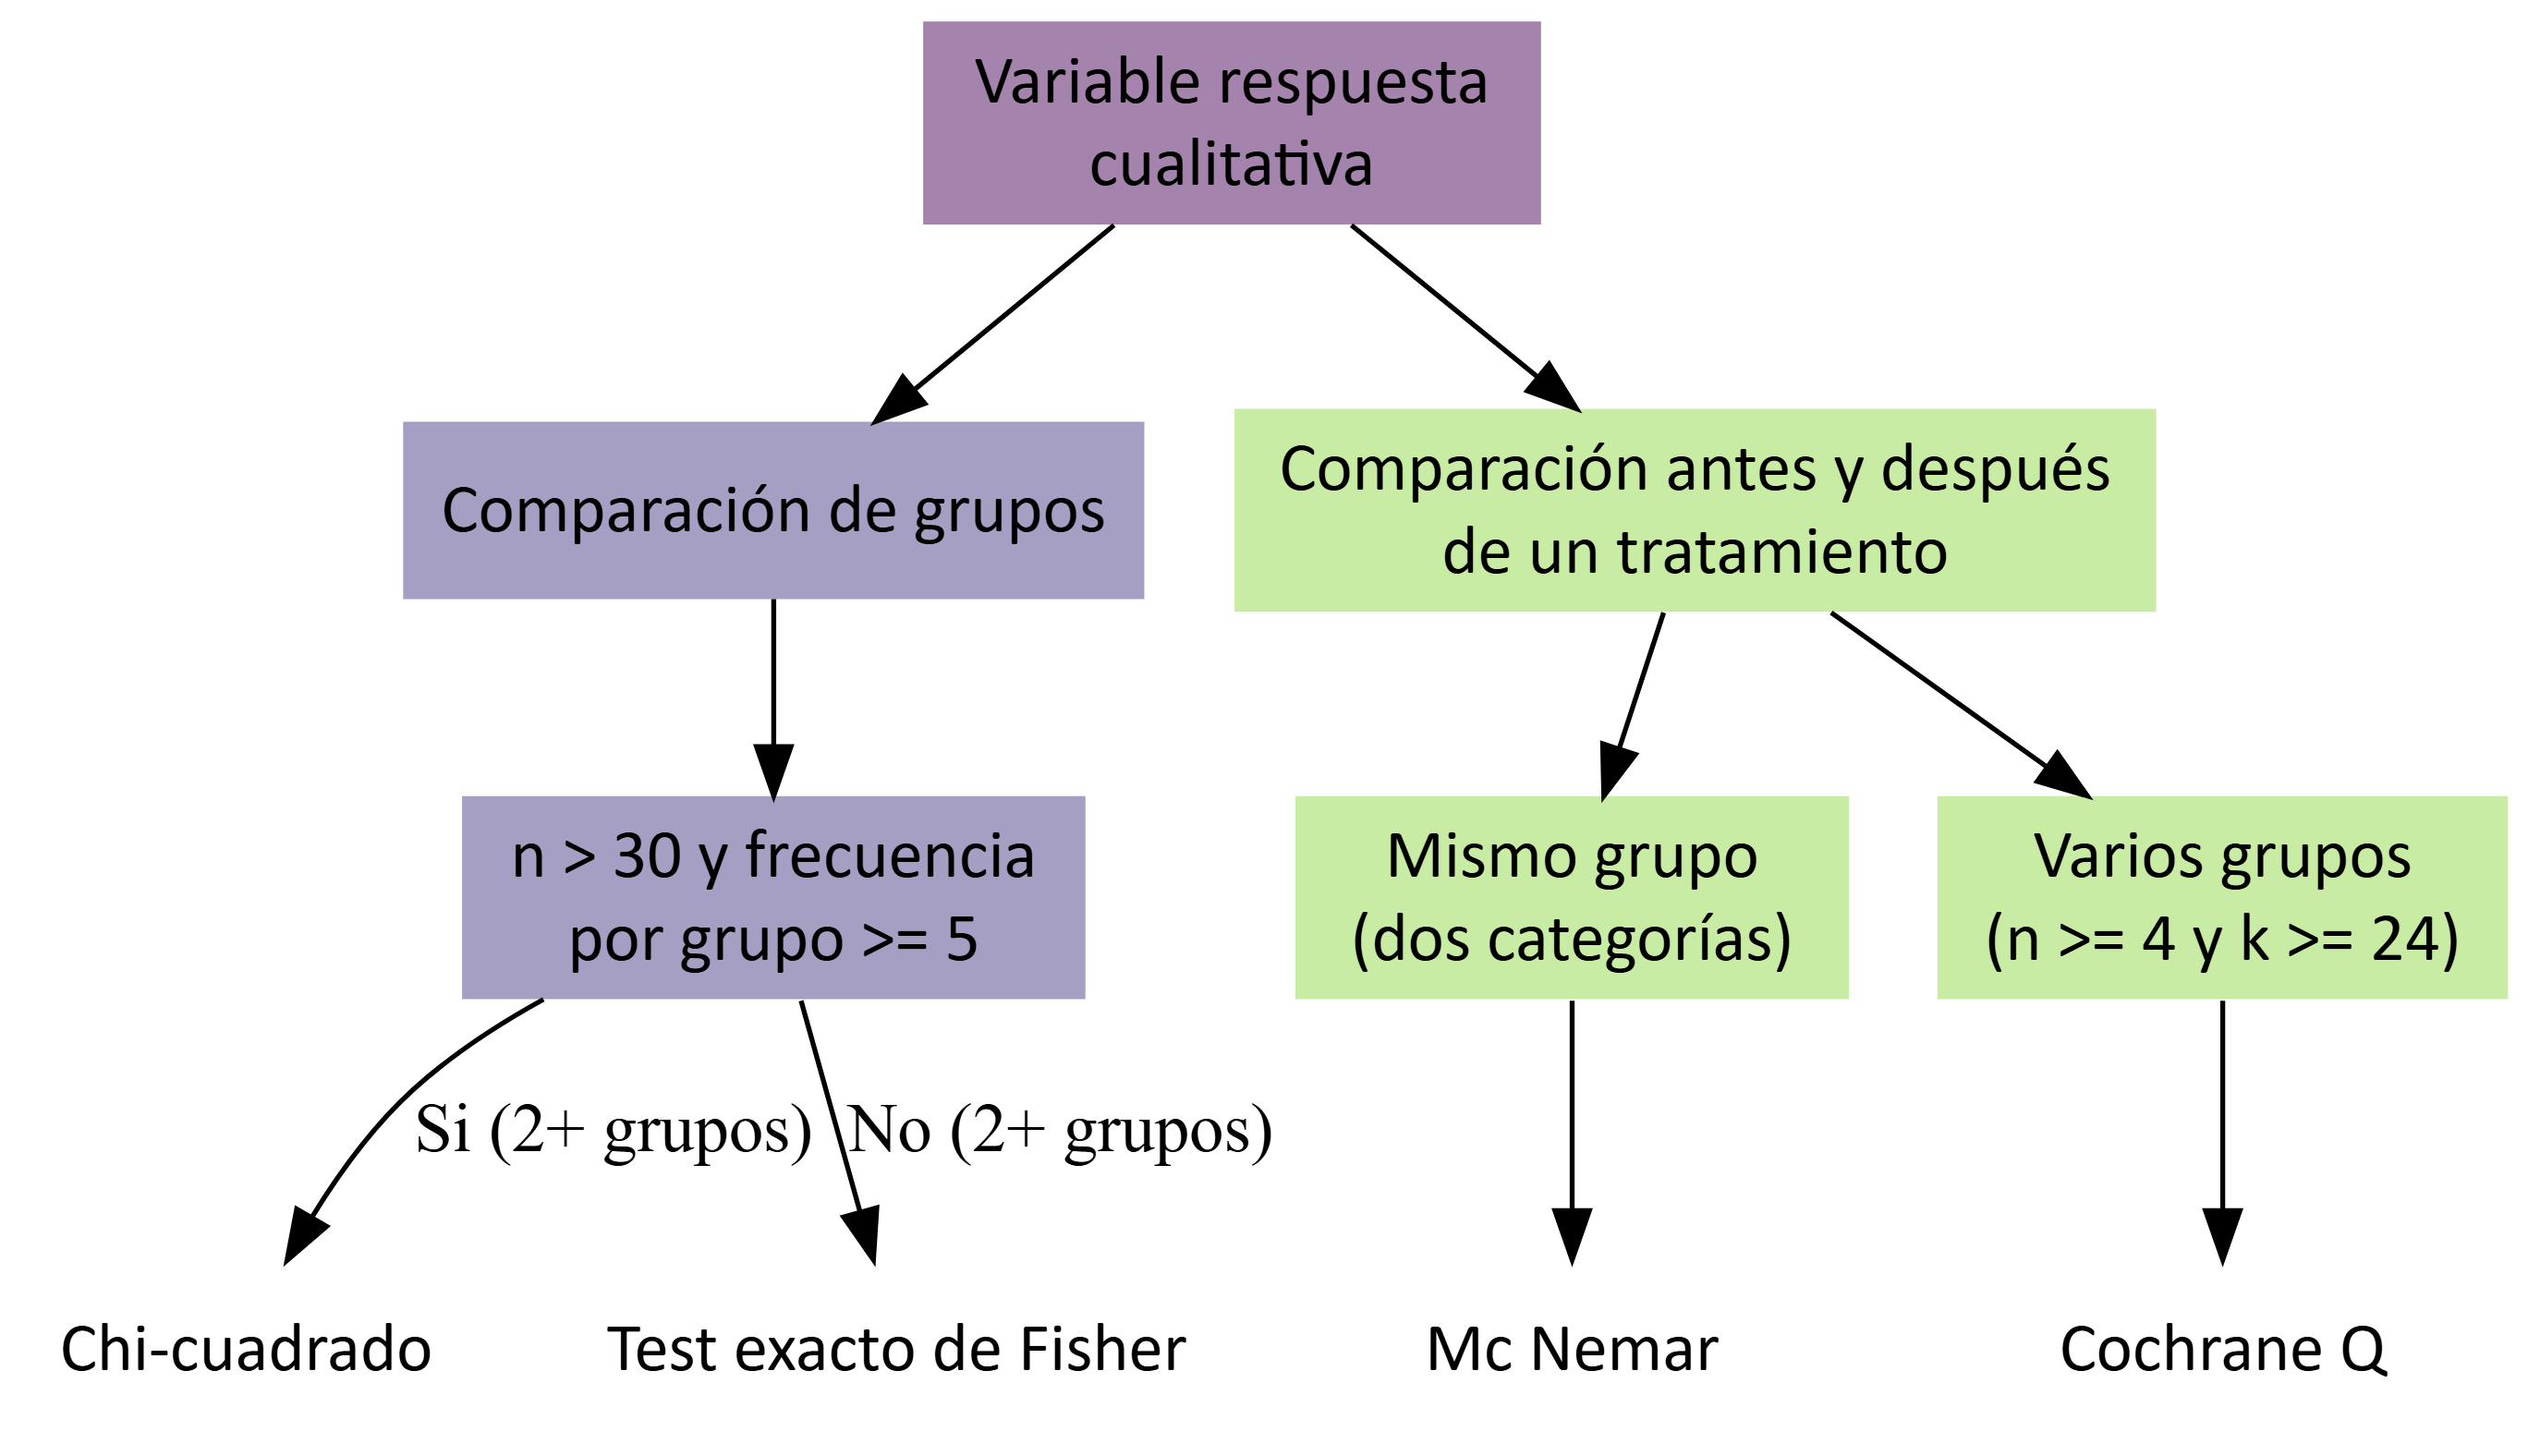
\includegraphics[width=5.5in,height=3.5in]{unidad_2/03_inferencia_files/figure-latex/dot-figure-5.png}

\section{Ejemplo práctico en R}\label{ejemplo-pruxe1ctico-en-r}

En el archivo ``\texttt{bebe1.txt}'' se encuentran datos de una muestra
aleatoria de los pesos al nacer de 186 bebés cuyas madres no consumieron
cocaína durante el embarazo. En el archivo ``\texttt{bebe2.txt}'' se
encuentran datos de una muestra aleatoria de 190 bebés cuyas madres
consumieron cocaína durante el embarazo. Nos interesa conocer el peso
promedio al nacer de los bebés de la primer base de datos y, de acuerdo
a estos resultados, saber si el consumo de cocaína afecta el peso que
tiene un bebé al nacer.

Podemos resolver la primer parte manualmente:

\[ 
IC = \bar{x} \pm Z_{1-\alpha/2}\frac{\sigma}{\sqrt{n}} 
\]

donde:

\begin{itemize}
\item
  media (\(\bar{x}\)): 3103 gramos
\item
  desvío estándar (\(\sigma\)): 696
\item
  número de observaciones (\(n\)): 186
\end{itemize}

\[ 
IC = 3103 \pm 2,57\frac{696}{\sqrt{186}} = 3103 \pm 131,16 
\]

\[
IC = 2971,85 - 3234,15
\]

El peso medio al nacer de los bebés oscila entre 2971,85 y 3234,15
gramos (\(\alpha = 0,99\)).

Para resolver las preguntas en R, comenzaremos cargando los paquetes
necesarios:

\begin{Shaded}
\begin{Highlighting}[]
\FunctionTok{library}\NormalTok{(tidyverse)}
\FunctionTok{library}\NormalTok{(dlookr)}
\end{Highlighting}
\end{Shaded}

Cargamos los datos:

\begin{Shaded}
\begin{Highlighting}[]
\NormalTok{datos1 }\OtherTok{\textless{}{-}} \FunctionTok{read\_csv2}\NormalTok{(}\StringTok{"datos/bebe1.txt"}\NormalTok{)}

\NormalTok{datos2 }\OtherTok{\textless{}{-}} \FunctionTok{read\_csv2}\NormalTok{(}\StringTok{"datos/bebe2.txt"}\NormalTok{)}
\end{Highlighting}
\end{Shaded}

La función \texttt{t.test()} del paquete \texttt{base} utiliza la
distribución \(t\) \emph{de Student}:

\begin{Shaded}
\begin{Highlighting}[]
\FunctionTok{t.test}\NormalTok{(datos1, }\AttributeTok{conf.level =} \FloatTok{0.99}\NormalTok{)}
\end{Highlighting}
\end{Shaded}

\begin{verbatim}

    One Sample t-test

data:  datos1
t = 60.804, df = 185, p-value < 2.2e-16
alternative hypothesis: true mean is not equal to 0
99 percent confidence interval:
 2970.178 3235.822
sample estimates:
mean of x 
     3103 
\end{verbatim}

Los IC producidos son similares a los calculados manualmente.

Para comparar los datos de los bebés de madres que consumieron cocaína,
debemos realizar un test de comparación de medias para dos poblaciones
independientes. Para ello, comenzamos por chequear normalidad:

\begin{Shaded}
\begin{Highlighting}[]
\FunctionTok{shapiro.test}\NormalTok{(datos1}\SpecialCharTok{$}\NormalTok{peso)}
\end{Highlighting}
\end{Shaded}

\begin{verbatim}

    Shapiro-Wilk normality test

data:  datos1$peso
W = 0.99293, p-value = 0.5092
\end{verbatim}

\begin{Shaded}
\begin{Highlighting}[]
\NormalTok{datos1 }\SpecialCharTok{|\textgreater{}}
  \FunctionTok{plot\_normality}\NormalTok{()}
\end{Highlighting}
\end{Shaded}

\begin{center}
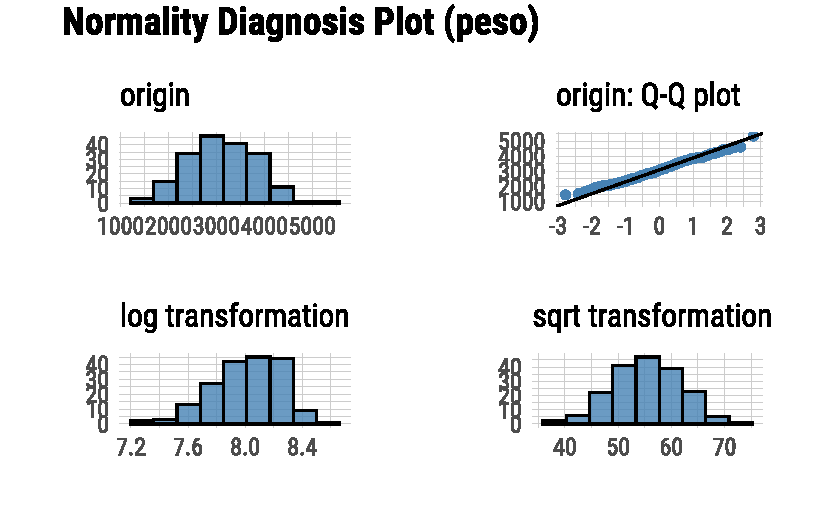
\includegraphics[width=0.85\linewidth,height=\textheight,keepaspectratio]{unidad_2/03_inferencia_files/figure-pdf/ej4-1.pdf}
\end{center}

\begin{Shaded}
\begin{Highlighting}[]
\FunctionTok{shapiro.test}\NormalTok{(datos2}\SpecialCharTok{$}\NormalTok{peso)}
\end{Highlighting}
\end{Shaded}

\begin{verbatim}

    Shapiro-Wilk normality test

data:  datos2$peso
W = 0.98951, p-value = 0.1774
\end{verbatim}

\begin{Shaded}
\begin{Highlighting}[]
\NormalTok{datos2 }\SpecialCharTok{|\textgreater{}}
  \FunctionTok{plot\_normality}\NormalTok{()}
\end{Highlighting}
\end{Shaded}

\begin{center}
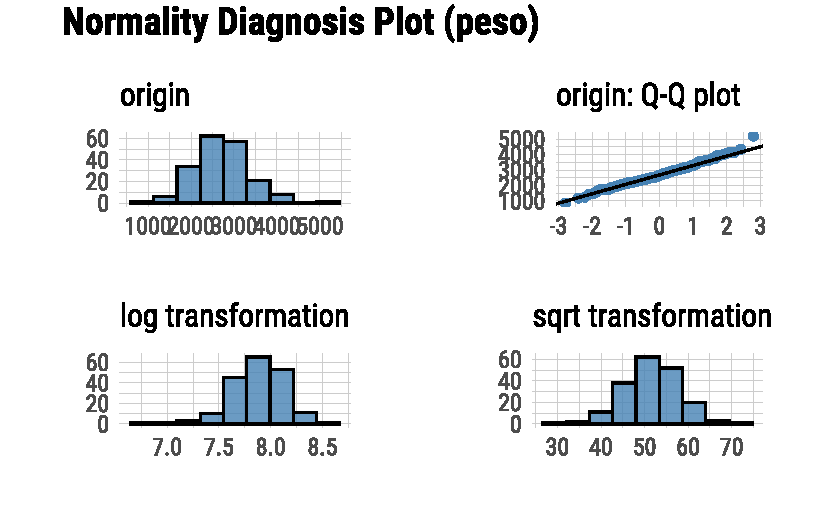
\includegraphics[width=0.85\linewidth,height=\textheight,keepaspectratio]{unidad_2/03_inferencia_files/figure-pdf/ej4-2.pdf}
\end{center}

Se cumple con el supuesto de normalidad, ahora procedemos a comparar
varianzas usando la función \texttt{var.test()}:

\begin{Shaded}
\begin{Highlighting}[]
\FunctionTok{var.test}\NormalTok{(datos1}\SpecialCharTok{$}\NormalTok{peso, datos2}\SpecialCharTok{$}\NormalTok{peso)}
\end{Highlighting}
\end{Shaded}

\begin{verbatim}

    F test to compare two variances

data:  datos1$peso and datos2$peso
F = 1.1644, num df = 185, denom df = 189, p-value = 0.2986
alternative hypothesis: true ratio of variances is not equal to 1
95 percent confidence interval:
 0.8736082 1.5526583
sample estimates:
ratio of variances 
          1.164392 
\end{verbatim}

Como las varianzas son iguales, aplicamos un \(t\) test para comparar
medias de dos poblaciones independientes con varianzas iguales
planteando un contraste bilateral:

\[
H_0: \mu_1 = \mu_2 \\
H_1: \mu_1 \neq \mu_2
\]

\begin{Shaded}
\begin{Highlighting}[]
\FunctionTok{t.test}\NormalTok{(}
       \AttributeTok{x =}\NormalTok{ datos1}\SpecialCharTok{$}\NormalTok{peso,}
       \AttributeTok{y =}\NormalTok{ datos2}\SpecialCharTok{$}\NormalTok{peso,}
       \AttributeTok{alternative =} \StringTok{"two.sided"}\NormalTok{,}
       \AttributeTok{var.equal =} \ConstantTok{TRUE}
\NormalTok{)}
\end{Highlighting}
\end{Shaded}

\begin{verbatim}

    Two Sample t-test

data:  datos1$peso and datos2$peso
t = 5.8252, df = 374, p-value = 1.231e-08
alternative hypothesis: true difference in means is not equal to 0
95 percent confidence interval:
 266.9644 539.0356
sample estimates:
mean of x mean of y 
     3103      2700 
\end{verbatim}

O también podríamos plantear un contraste unilateral, si consideramos
que nuestra hipótesis de trabajo es que el peso de los bebés de madres
que no consumen cocaína es mayor que aquellos de madres que sí consumen.

\[
H_0: \mu_1 = \mu_2 \\
H_1: \mu_1 > \mu_2 \quad ó \quad \mu_1 - \mu_2 > 0
\]

\begin{Shaded}
\begin{Highlighting}[]
\FunctionTok{t.test}\NormalTok{(}
       \AttributeTok{x =}\NormalTok{ datos1}\SpecialCharTok{$}\NormalTok{peso,}
       \AttributeTok{y =}\NormalTok{ datos2}\SpecialCharTok{$}\NormalTok{peso,}
       \AttributeTok{alternative =} \StringTok{"greater"}\NormalTok{,}
       \AttributeTok{var.equal =} \ConstantTok{TRUE}
\NormalTok{)}
\end{Highlighting}
\end{Shaded}

\begin{verbatim}

    Two Sample t-test

data:  datos1$peso and datos2$peso
t = 5.8252, df = 374, p-value = 6.155e-09
alternative hypothesis: true difference in means is greater than 0
95 percent confidence interval:
 288.9222      Inf
sample estimates:
mean of x mean of y 
     3103      2700 
\end{verbatim}

Concluimos que los pesos de los bebés hijos de madres que no consumen
cocaína es significativamente mayor respecto de los hijos de madres que
sí la consumen.

\subsection{Inferencia sobre una
población}\label{inferencia-sobre-una-poblaciuxf3n}

En algunas situaciones, además de obtener intervalos de confianza para
estimar parámetros como la media o la proporción poblacional, también
puede ser de interés realizar contrastes de hipótesis sobre un valor
específico de referencia. Este tipo de análisis se denomina
\textbf{inferencia sobre una población} y permite evaluar si un
parámetro poblacional es significativamente diferente de un valor dado.

Un caso común en epidemiología y medicina es el estudio de la eficacia
de un tratamiento. Supongamos que queremos evaluar si un nuevo fármaco
reduce la presión arterial en pacientes con un determinado síndrome. Se
sabe que, en ausencia de tratamiento, la presión arterial media en estos
pacientes es de \textbf{165 mmHg}. Para investigar el efecto del
fármaco, se administra a un grupo de \textbf{15 pacientes} y se mide su
presión arterial después del tratamiento.

Queremos evaluar si la presión arterial media en pacientes tratados con
el nuevo fármaco es \textbf{significativamente menor} que la presión
arterial histórica de 165 mmHg:

\begin{itemize}
\item
  \(H_0: \mu = 165~mmHg\)
\item
  \(H_1: \mu < 165~mmHg\)
\end{itemize}

Este es un \textbf{contraste unilateral a la izquierda}, ya que buscamos
evidencia de que el tratamiento reduce la presión arterial.

Cargamos los datos:

\begin{Shaded}
\begin{Highlighting}[]
\NormalTok{enfermos }\OtherTok{\textless{}{-}} \FunctionTok{read\_csv2}\NormalTok{(}\StringTok{"datos/enfermos.txt"}\NormalTok{)}
\end{Highlighting}
\end{Shaded}

Calculamos la media y el desvío estándar:

\begin{Shaded}
\begin{Highlighting}[]
\NormalTok{enfermos }\SpecialCharTok{|\textgreater{}}
  \FunctionTok{summarise}\NormalTok{(}\AttributeTok{media =} \FunctionTok{mean}\NormalTok{(V1), }\AttributeTok{desvio =} \FunctionTok{sd}\NormalTok{(V1))}
\end{Highlighting}
\end{Shaded}

\begin{verbatim}
# A tibble: 1 x 2
  media desvio
  <dbl>  <dbl>
1  152.   22.0
\end{verbatim}

Evaluamos normalidad:

\begin{Shaded}
\begin{Highlighting}[]
\FunctionTok{shapiro.test}\NormalTok{(enfermos}\SpecialCharTok{$}\NormalTok{V1)}
\end{Highlighting}
\end{Shaded}

\begin{verbatim}

    Shapiro-Wilk normality test

data:  enfermos$V1
W = 0.94967, p-value = 0.5192
\end{verbatim}

Este grupo de enfermos tratados con el nuevo fármaco tienen una media de
aproximadamente 151.9619928, con un desvío de 21.9788237. Además, los
datos cumplen con el supuesto de normalidad.

Realizamos la prueba de hipótesis para evaluar si este valor es
significativamente menor a 165:

\begin{Shaded}
\begin{Highlighting}[]
\FunctionTok{t.test}\NormalTok{(}\AttributeTok{x =}\NormalTok{ enfermos}\SpecialCharTok{$}\NormalTok{V1, }\AttributeTok{alternative =} \StringTok{"less"}\NormalTok{, }\AttributeTok{mu =} \DecValTok{165}\NormalTok{, }\AttributeTok{conf.level =} \FloatTok{0.95}\NormalTok{)}
\end{Highlighting}
\end{Shaded}

\begin{verbatim}

    One Sample t-test

data:  enfermos$V1
t = -2.2975, df = 14, p-value = 0.01876
alternative hypothesis: true mean is less than 165
95 percent confidence interval:
     -Inf 161.9573
sample estimates:
mean of x 
  151.962 
\end{verbatim}

Dado que \(p < 0.05\), rechazamos la hipótesis nula y concluimos que,
con un nivel de confianza del 95\%, el nuevo fármaco \textbf{reduce
significativamente la presión arterial} en estos pacientes.

Rodríguez y Mendivelso (2018)

Hernández-Ávila (2011)

Álvarez Cáceres (2007)

Triola (2018)

Rodríguez et~al. (2003)

Norman, GR y Streiner, DL (1996)

Ríus Díaz et~al. (2012)

Daniel (2002)

Glantz, S (2006)

Ryu (2025)

Manitz et~al. (2021)

\emph{{EPIDAT} 4.2 - {Consellería} de {Sanidade} - {Servizo} {Galego} de
{Saúde}} (s.~f.)

\section*{Referencias}\label{referencias-6}
\addcontentsline{toc}{section}{Referencias}

\markright{Referencias}

\chapter{Análisis de normalidad y
homocedasticidad}\label{anuxe1lisis-de-normalidad-y-homocedasticidad}

\section{Introducción}\label{introducciuxf3n-6}

Este material es una continuación del capítulo sobre \textbf{Análisis
exploratorio de datos} de la \textbf{Unidad 1}. Recordemos que uno de
los objetivos del EDA es conocer cómo se distribuyen los valores de las
variables de interés.

Las características fundamentales a la hora de decidir si utilizaremos
métodos paramétricos o no paramétricos para la inferencia estadística,
es que los datos se ajusten a una distribución normal y conocer si
tienen una dispersión homogénea o heterogénea. Ahora que conocemos el
funcionamiento interno de los test de hipótesis, podemos usar
\textbf{pruebas de bondad de ajuste} para evaluar los supuestos de
normalidad y homocedasticidad.

\section{Normalidad}\label{normalidad}

Determinar que una distribución es aproximadamente normal nos permite
decidirnos por test de comparaciones paramétricos.

Existen tres enfoques que debemos analizar simultáneamente:

\begin{itemize}
\tightlist
\item
  Métodos gráficos
\item
  Métodos analíticos
\item
  Pruebas de bondad de ajuste
\end{itemize}

\subsection{Métodos gráficos}\label{muxe9todos-gruxe1ficos}

El gráfico por excelencia para evaluar normalidad es el Q-Q Plot que
consiste en comparar los cuantiles de la distribución observada con los
cuantiles teóricos de una distribución normal con la misma media y
desviación estándar que los datos.

Cuanto más se aproximen los datos a una normal, más alineados están los
puntos entorno a la recta.

En el lenguaje R hay varios paquetes que tienen funciones para
construirlos:

\begin{Shaded}
\begin{Highlighting}[]
\FunctionTok{library}\NormalTok{(dlookr)}
\FunctionTok{library}\NormalTok{(ggpubr)}
\FunctionTok{library}\NormalTok{(moments)}
\FunctionTok{library}\NormalTok{(nortest)}
\FunctionTok{library}\NormalTok{(car)}
\FunctionTok{library}\NormalTok{(tidyverse)}
\end{Highlighting}
\end{Shaded}

Cargamos datos de ejemplo:

\begin{Shaded}
\begin{Highlighting}[]
\NormalTok{datos }\OtherTok{\textless{}{-}} \FunctionTok{read\_csv2}\NormalTok{(}\StringTok{"datos/datos\_normalidad.csv"}\NormalTok{)}
\end{Highlighting}
\end{Shaded}

Evaluación gráfica de normalidad usando la función
\texttt{plot\_normality()} del paquete \texttt{dlookr}:

\begin{Shaded}
\begin{Highlighting}[]
\NormalTok{datos }\SpecialCharTok{|\textgreater{}}
  \FunctionTok{plot\_normality}\NormalTok{(peso)}
\end{Highlighting}
\end{Shaded}

\begin{center}
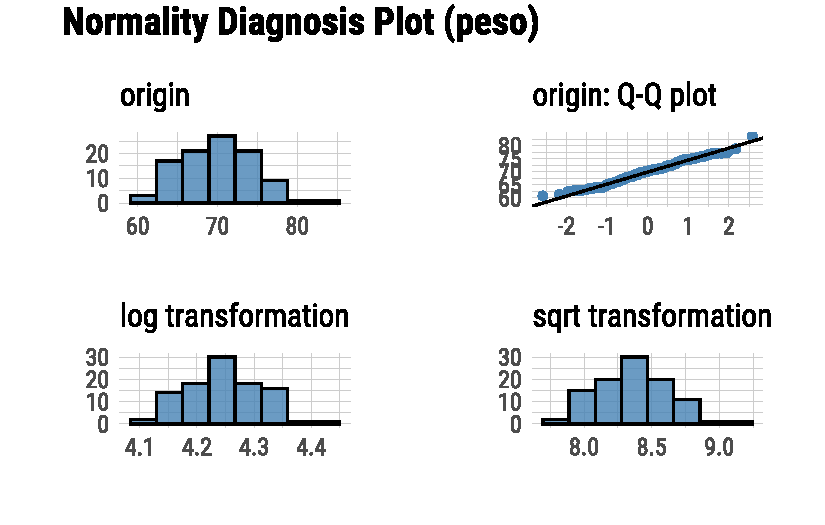
\includegraphics[width=0.85\linewidth,height=\textheight,keepaspectratio]{unidad_2/04_norm_het_files/figure-pdf/cod3-1.pdf}
\end{center}

A simple vista observamos que los puntos de la variable \texttt{peso}
\emph{se ajustan bastante bien a la recta}.

También podemos generar el qqplot usando las funciones
\texttt{geom\_qq\_line()} y \texttt{geom\_qq()} de \texttt{ggplot2}:

\begin{Shaded}
\begin{Highlighting}[]
\NormalTok{datos }\SpecialCharTok{|\textgreater{}}
  \FunctionTok{ggplot}\NormalTok{(}\AttributeTok{mapping =} \FunctionTok{aes}\NormalTok{(}\AttributeTok{sample =}\NormalTok{ peso)) }\SpecialCharTok{+}
  \FunctionTok{geom\_qq\_line}\NormalTok{() }\SpecialCharTok{+}
  \FunctionTok{geom\_qq}\NormalTok{() }\SpecialCharTok{+}
  \FunctionTok{theme\_minimal}\NormalTok{()}
\end{Highlighting}
\end{Shaded}

\begin{center}
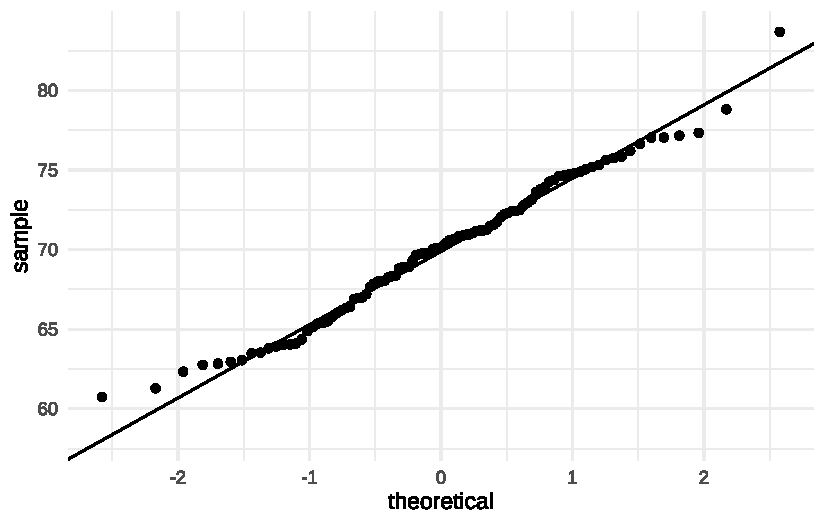
\includegraphics[width=0.85\linewidth,height=\textheight,keepaspectratio]{unidad_2/04_norm_het_files/figure-pdf/cod4-1.pdf}
\end{center}

La función \texttt{ggqqplot()} del paquete \texttt{ggpubr} (Kassambara
2026a) nos permite agregar intervalos de confianza (zona gris alrededor
de la recta) que nos orienta mejor sobre ``donde caen'' los puntos de la
variable analizada:

\begin{Shaded}
\begin{Highlighting}[]
\NormalTok{datos}\SpecialCharTok{$}\NormalTok{peso }\SpecialCharTok{|\textgreater{}}
  \FunctionTok{ggqqplot}\NormalTok{()}
\end{Highlighting}
\end{Shaded}

\begin{center}
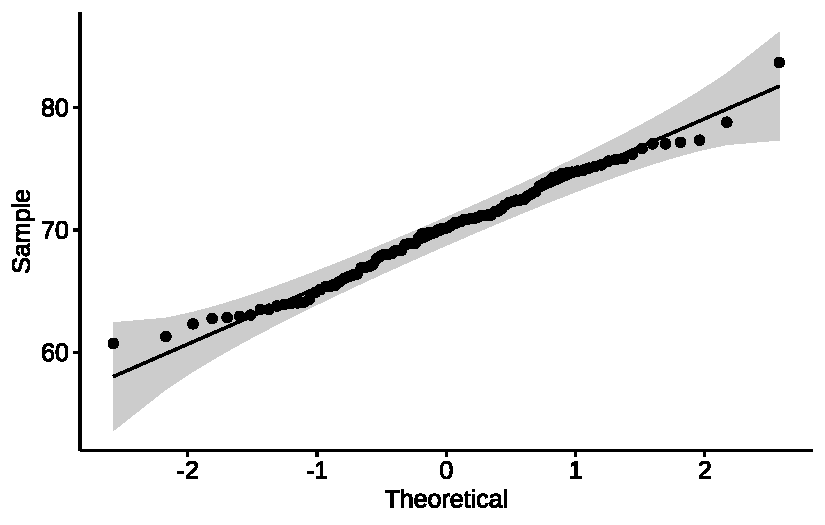
\includegraphics[width=0.85\linewidth,height=\textheight,keepaspectratio]{unidad_2/04_norm_het_files/figure-pdf/cod5-1.pdf}
\end{center}

Un ejemplo donde la variable parece no cumplir con el supuesto de
normalidad en estos datos de prueba es \texttt{edad}:

\begin{Shaded}
\begin{Highlighting}[]
\NormalTok{datos}\SpecialCharTok{$}\NormalTok{edad }\SpecialCharTok{|\textgreater{}}
  \FunctionTok{ggqqplot}\NormalTok{()}
\end{Highlighting}
\end{Shaded}

\begin{center}
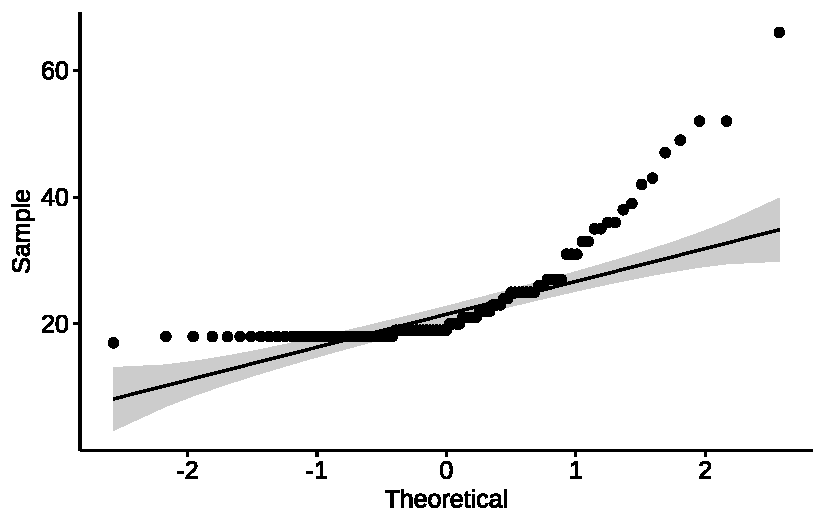
\includegraphics[width=0.85\linewidth,height=\textheight,keepaspectratio]{unidad_2/04_norm_het_files/figure-pdf/cod6-1.pdf}
\end{center}

\subsection{Métodos analíticos}\label{muxe9todos-analuxedticos}

\subsubsection{Medidas de forma}\label{medidas-de-forma}

Existen dos medidas de forma útiles que podemos calcular mediante
funciones de R.

\begin{itemize}
\tightlist
\item
  La curtosis (kurtosis)
\item
  La asimetría (skewness)
\end{itemize}

La curtosis mide el grado de agudeza o achatamiento de una distribución
con relación a la distribución normal.

\begin{itemize}
\tightlist
\item
  \(< 0\) Distribución platicúrtica (apuntamiento negativo): baja
  concentración de valores
\item
  \(> 0\) Distribución leptocúrtica (apuntamiento positivo): gran
  concentración de valores
\item
  \(= 0\) Distribución mesocúrtica (apuntamiento normal): concentración
  como en la distribución normal.
\end{itemize}

El paquete \texttt{moments} (Komsta y Novomestky 2022) posee algunas
funciones interesantes para analizar medidas de forma, como el estimador
de Pearson para curtosis:

\begin{Shaded}
\begin{Highlighting}[]
\NormalTok{datos }\SpecialCharTok{|\textgreater{}}
  \FunctionTok{summarise}\NormalTok{(}
    \AttributeTok{kurtosis\_edad =} \FunctionTok{kurtosis}\NormalTok{(edad, }\AttributeTok{na.rm =}\NormalTok{ T),}
    \AttributeTok{kurtosis\_peso =} \FunctionTok{kurtosis}\NormalTok{(peso, }\AttributeTok{na.rm =}\NormalTok{ T)}
\NormalTok{  )}
\end{Highlighting}
\end{Shaded}

\begin{verbatim}
# A tibble: 1 x 2
  kurtosis_edad kurtosis_peso
          <dbl>         <dbl>
1          8.05          2.72
\end{verbatim}

En los dos casos estamos frente a una \emph{distribución leptocúrtica}
pero de magnitudes bien diferentes. Muy alta en el caso de la variable
\texttt{edad} (8,0) y mucho menor para la variable \texttt{peso} (2,7).

El índice de asimetría es un indicador que permite establecer el
\emph{grado de asimetría} que presenta una distribución. Los valores
menores que 0 indican distribución asimétrica negativa; los mayores a 0:
distribución asimétrica positiva y cuando sea 0, o muy próximo a 0,
distribución simétrica:

\begin{Shaded}
\begin{Highlighting}[]
\NormalTok{datos }\SpecialCharTok{|\textgreater{}}
  \FunctionTok{summarise}\NormalTok{(}
    \AttributeTok{asimetria\_edad =} \FunctionTok{skewness}\NormalTok{(edad, }\AttributeTok{na.rm =}\NormalTok{ T),}
    \AttributeTok{asimetria\_peso =} \FunctionTok{skewness}\NormalTok{(peso, }\AttributeTok{na.rm =}\NormalTok{ T)}
\NormalTok{  )}
\end{Highlighting}
\end{Shaded}

\begin{verbatim}
# A tibble: 1 x 2
  asimetria_edad asimetria_peso
           <dbl>          <dbl>
1           2.19          0.122
\end{verbatim}

Los valores obtenidos con la función \texttt{skewness()} del paquete
\texttt{moments} nos informan que la distribución de la edad tienen una
asimetría positiva (2,2) y que los valores de peso se distribuyen
bastante simétricos (0,1).

Estas características de las distribuciones también se pueden ver
mediante histogramas o gráficos de densidad:

\begin{Shaded}
\begin{Highlighting}[]
\NormalTok{datos }\SpecialCharTok{|\textgreater{}}
  \FunctionTok{plot\_normality}\NormalTok{(edad, }\AttributeTok{col =} \StringTok{"forestgreen"}\NormalTok{)}
\end{Highlighting}
\end{Shaded}

\begin{center}
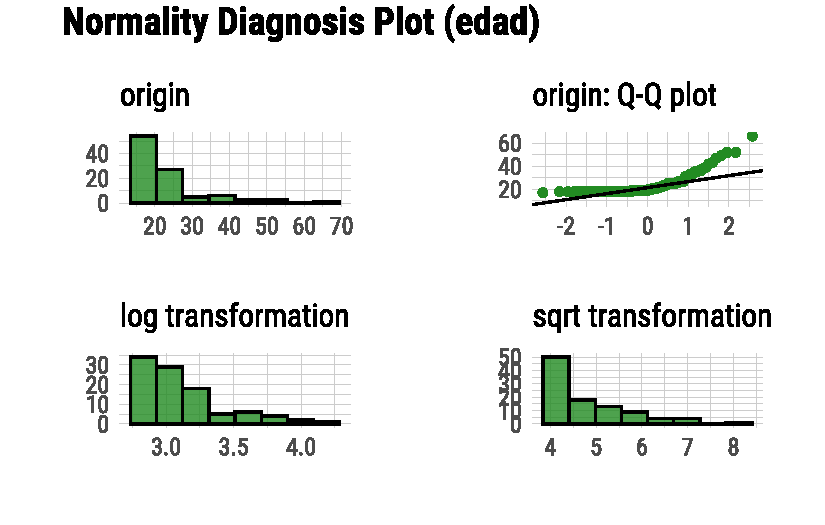
\includegraphics[width=0.85\linewidth,height=\textheight,keepaspectratio]{unidad_2/04_norm_het_files/figure-pdf/cod9-1.pdf}
\end{center}

\begin{Shaded}
\begin{Highlighting}[]
\NormalTok{datos }\SpecialCharTok{|\textgreater{}}
  \FunctionTok{plot\_normality}\NormalTok{(peso, }\AttributeTok{col =} \StringTok{"royalblue"}\NormalTok{)}
\end{Highlighting}
\end{Shaded}

\begin{center}
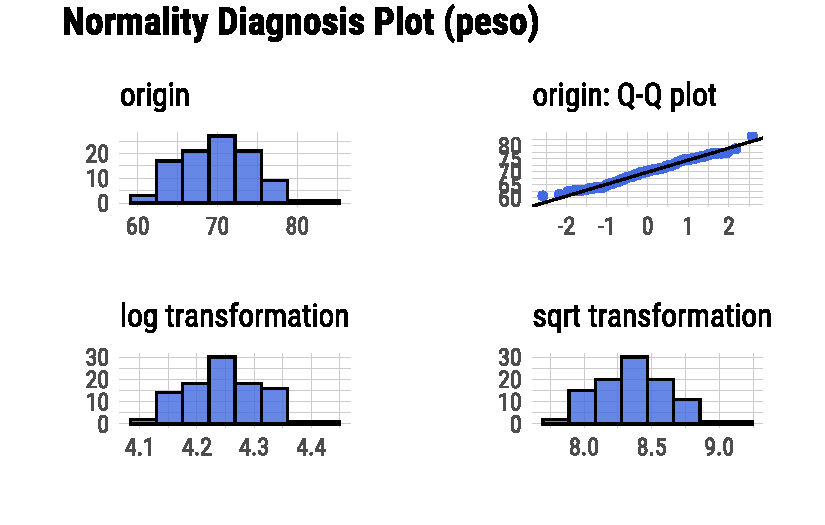
\includegraphics[width=0.85\linewidth,height=\textheight,keepaspectratio]{unidad_2/04_norm_het_files/figure-pdf/cod9-2.pdf}
\end{center}

Los histogramas que se acerquen a la clásica ``campana de Gauss''
tendrán curtosis y asimetrías alrededor del valor cero.

\subsection{Pruebas de bondad de
ajuste}\label{pruebas-de-bondad-de-ajuste}

Una prueba de bondad de ajuste permite testear la hipótesis de que una
variable aleatoria sigue cierta distribución de probabilidad y se
utiliza en situaciones donde se requiere comparar una distribución
observada con una teórica o hipotética.

El mecanismo es idéntico a cualquier test de hipótesis salvo que aquí
esperamos no descartar la hipótesis nula de igualdad, por lo que obtener
valores \emph{p} de probabilidad mayores a 0,05 es signo de que la
distribución de la variable analizada se ajusta.

A continuación, presentaremos los test de hipótesis más utilizados para
analizar normalidad.

\subsubsection{Test de Shapiro-Wilk}\label{test-de-shapiro-wilk}

Lleva el nombre de sus autores (Samuel Shapiro y Martin Wilk) y es usado
preferentemente para muestras de hasta 50 observaciones.

La función se encuentra desarrollada en el paquete \texttt{stats} y se
llama \texttt{shapiro.test()}:

\begin{Shaded}
\begin{Highlighting}[]
\FunctionTok{shapiro.test}\NormalTok{(datos}\SpecialCharTok{$}\NormalTok{edad)}
\end{Highlighting}
\end{Shaded}

\begin{verbatim}

    Shapiro-Wilk normality test

data:  datos$edad
W = 0.69517, p-value = 4.912e-13
\end{verbatim}

\begin{Shaded}
\begin{Highlighting}[]
\FunctionTok{shapiro.test}\NormalTok{(datos}\SpecialCharTok{$}\NormalTok{peso)}
\end{Highlighting}
\end{Shaded}

\begin{verbatim}

    Shapiro-Wilk normality test

data:  datos$peso
W = 0.98615, p-value = 0.383
\end{verbatim}

\textbf{Interpretación}: Siendo la hipótesis nula que la población está
distribuida normalmente, si el p-valor es menor a \(\alpha\) (nivel de
significancia, convencionalmente un 0,05) entonces la hipótesis nula es
rechazada (se concluye que los datos no provienen de una distribución
normal). Si el p-valor es mayor a \(\alpha\), se concluye que no se
puede rechazar dicha hipótesis.

En función de esta interpretación (que es común a todos los test de
hipótesis de normalidad), podemos decir que la distribución de la
variable \textbf{edad} \emph{no se ajusta a la normal} y no podemos
rechazar que la distribución de la variable \textbf{peso} se ajuste.

\subsubsection{Test de
Kolmogorov-Smirnov}\label{test-de-kolmogorov-smirnov}

El test de \textbf{Kolmogorov-Smirnov} permite estudiar si una muestra
procede de una población con una determinada distribución que no está
limitado únicamente a la distribución normal.

El test asume que se conoce la media y varianza poblacional, lo que en
la mayoría de los casos no es posible. Para resolver este problema, se
realizó una modificación conocida como test Lilliefors.

\subsubsection{Test de Lilliefors}\label{test-de-lilliefors}

El test de \textbf{Lilliefors} asume que la media y varianza son
desconocidas y está especialmente desarrollado para contrastar la
normalidad.

Es la alternativa al test de Shapiro-Wilk cuando el número de
observaciones es mayor de 50.

La función \texttt{lillie.test()} del paquete \texttt{nortest} (Gross y
Ligges 2015) permite aplicarlo:

\begin{Shaded}
\begin{Highlighting}[]
\FunctionTok{lillie.test}\NormalTok{(datos}\SpecialCharTok{$}\NormalTok{edad)}
\end{Highlighting}
\end{Shaded}

\begin{verbatim}

    Lilliefors (Kolmogorov-Smirnov) normality test

data:  datos$edad
D = 0.24892, p-value < 2.2e-16
\end{verbatim}

\begin{Shaded}
\begin{Highlighting}[]
\FunctionTok{lillie.test}\NormalTok{(datos}\SpecialCharTok{$}\NormalTok{peso)}
\end{Highlighting}
\end{Shaded}

\begin{verbatim}

    Lilliefors (Kolmogorov-Smirnov) normality test

data:  datos$peso
D = 0.049534, p-value = 0.7905
\end{verbatim}

Los resultados son coincidentes con los obtenidos anteriormente.

\subsubsection{Test de D'agostino}\label{test-de-dagostino}

Esta prueba se basa en las transformaciones de la curtosis y la
asimetría de la muestra, y solo tiene poder frente a las alternativas de
que la distribución sea sesgada.

El paquete \texttt{moments} la tiene implementada en
\texttt{agostino.test()}:

\begin{Shaded}
\begin{Highlighting}[]
\FunctionTok{agostino.test}\NormalTok{(datos}\SpecialCharTok{$}\NormalTok{edad)}
\end{Highlighting}
\end{Shaded}

\begin{verbatim}

    D'Agostino skewness test

data:  datos$edad
skew = 2.1947, z = 6.3465, p-value = 2.203e-10
alternative hypothesis: data have a skewness
\end{verbatim}

\begin{Shaded}
\begin{Highlighting}[]
\FunctionTok{agostino.test}\NormalTok{(datos}\SpecialCharTok{$}\NormalTok{peso)}
\end{Highlighting}
\end{Shaded}

\begin{verbatim}

    D'Agostino skewness test

data:  datos$peso
skew = 0.12160, z = 0.52683, p-value = 0.5983
alternative hypothesis: data have a skewness
\end{verbatim}

Los resultados coinciden con la observación de asimetría que efectuamos
con los métodos analíticos, confirmando que la variable \texttt{edad}
\emph{no se ajusta} a una curva simétrica y la variable \texttt{peso} si
lo hace.

Cuando estos test se emplean con la finalidad de verificar las
condiciones de métodos paramétricos es importante tener en cuenta que,
al tratarse de valores probabilidad, cuanto mayor sea el tamaño de la
muestra más poder estadístico tienen y más fácil es encontrar evidencias
en contra de la hipótesis nula de normalidad.

Por otra parte, cuanto mayor sea el tamaño de la muestra, menos
sensibles son los métodos paramétricos a la falta de normalidad. Por
esta razón, es importante no basar las conclusiones únicamente en los
resultados de los test, sino también considerar los otros métodos
(gráfico y analítico) y no olvidar el tamaño de la muestra.

\section{Homocedasticidad}\label{homocedasticidad}

La homogeneidad de varianzas es un supuesto que considera constante la
varianza en los distintos grupos que queremos comparar.

Esta homogeneidad es condición necesaria antes de aplicar algunos test
de hipótesis de comparaciones o bien para aplicar correcciones mediante
los argumentos de las funciones de R.

Existen diferentes test de bondad de ajuste que permiten evaluar la
distribución de la varianza. Todos ellos consideran como \(H_0\) que la
varianza es igual entre los grupos y como \(H_1\) que no lo es.

La diferencia entre ellos es el estadístico de centralidad que utilizan:

\begin{itemize}
\item
  Media de la varianza: son los más potentes pero se aplican en
  distribuciones que se aproximan a la normal.
\item
  Mediana de la varianza: son menos potentes pero consiguen mejores
  resultados en distribuciones asimétricas.
\end{itemize}

\subsection{F-test}\label{f-test}

Este test es un contraste de la razón de varianzas, mediante el
estadístico F que sigue una distribución F-Snedecor.

Se utiliza cuando las distribuciones se aproximan a la ``normal'' y en R
base se la encuentra en la función \texttt{var.test()} que permite
utilizar la sintaxis de fórmula:

\begin{Shaded}
\begin{Highlighting}[]
\NormalTok{variable\_cuantitativa }\SpecialCharTok{\textasciitilde{}}\NormalTok{ variable\_categórica\_grupos}
\end{Highlighting}
\end{Shaded}

Por ejemplo:

\begin{Shaded}
\begin{Highlighting}[]
\FunctionTok{var.test}\NormalTok{(}\AttributeTok{formula =}\NormalTok{ peso }\SpecialCharTok{\textasciitilde{}}\NormalTok{ sexo, }\AttributeTok{data =}\NormalTok{ datos)}
\end{Highlighting}
\end{Shaded}

\begin{verbatim}

    F test to compare two variances

data:  peso by sexo
F = 0.67914, num df = 50, denom df = 48, p-value = 0.1781
alternative hypothesis: true ratio of variances is not equal to 1
95 percent confidence interval:
 0.384712 1.194943
sample estimates:
ratio of variances 
         0.6791414 
\end{verbatim}

Comparamos las varianzas de la variable peso entre el grupo de mujeres y
hombres. El valor \(p\) del test indica que no podemos descartar la
igualdad de varianzas entre los grupos (\(H_0\)) o lo que es lo mismo el
test no encuentra diferencias significativas entre las varianzas de los
dos grupos.

\subsection{Test de Bartlett}\label{test-de-bartlett}

Este test se puede utilizar como alternativa al F-test, sobre todo
porque nos permite aplicarlo cuando tenemos más de 2 grupos de
comparación. Al igual que el anterior es sensible a las desviaciones de
la normalidad.

La función en R \texttt{base} es \texttt{bartlett.test()} y también se
pueden usar argumentos tipo fórmula:

\begin{Shaded}
\begin{Highlighting}[]
\FunctionTok{bartlett.test}\NormalTok{(}\AttributeTok{formula =}\NormalTok{ peso }\SpecialCharTok{\textasciitilde{}}\NormalTok{ sexo, }\AttributeTok{data =}\NormalTok{ datos)}
\end{Highlighting}
\end{Shaded}

\begin{verbatim}

    Bartlett test of homogeneity of variances

data:  peso by sexo
Bartlett's K-squared = 1.8082, df = 1, p-value = 0.1787
\end{verbatim}

El resultado es coincidente con el mostrado por \texttt{var.test()}. No
se encuentran diferencias significativas entres las varianzas de los
pesos en los dos grupos (Mujer - Varon)

\subsection{Test de Levene}\label{test-de-levene}

El test de Levene sirve para comparar la varianza de 2 o más grupos pero
además permite elegir distintos estadísticos de tendencia central. Por
lo tanto, la podemos adaptar a distribuciones alejadas de la normalidad
seleccionando por ejemplo la mediana.

La función \texttt{leveneTest()} se encuentra disponible en el paquete
\texttt{car}. La vemos aplicada sobre \texttt{peso} para los diferentes
grupos de \texttt{sexo} y utilizando la \textbf{media} como estadístico
de centralidad, dado que la distribución de \texttt{peso} se aproxima a
la normal.

\begin{Shaded}
\begin{Highlighting}[]
\FunctionTok{leveneTest}\NormalTok{(}\AttributeTok{y =}\NormalTok{ peso }\SpecialCharTok{\textasciitilde{}}\NormalTok{ sexo, }\AttributeTok{data =}\NormalTok{ datos, }\AttributeTok{center =} \StringTok{"mean"}\NormalTok{)}
\end{Highlighting}
\end{Shaded}

\begin{verbatim}
Levene's Test for Homogeneity of Variance (center = "mean")
      Df F value Pr(>F)
group  1       2 0.1605
      98               
\end{verbatim}

La conclusión es la misma que la encontrada anteriormente.

Ahora vamos aplicarla sobre la variable \texttt{edad}, de la que
habíamos descartado ``normalidad''. Lo hacemos usando el argumento
\texttt{center} con \texttt{"mean"} (media) y con \texttt{"median"}
(mediana).

\begin{Shaded}
\begin{Highlighting}[]
\FunctionTok{leveneTest}\NormalTok{(}\AttributeTok{y =}\NormalTok{ edad }\SpecialCharTok{\textasciitilde{}}\NormalTok{ sexo, }\AttributeTok{data =}\NormalTok{ datos, }\AttributeTok{center =} \StringTok{"mean"}\NormalTok{)}
\end{Highlighting}
\end{Shaded}

\begin{verbatim}
Levene's Test for Homogeneity of Variance (center = "mean")
      Df F value Pr(>F)  
group  1  4.6784  0.033 *
      97                 
---
Signif. codes:  0 '***' 0.001 '**' 0.01 '*' 0.05 '.' 0.1 ' ' 1
\end{verbatim}

\begin{Shaded}
\begin{Highlighting}[]
\FunctionTok{leveneTest}\NormalTok{(}\AttributeTok{y =}\NormalTok{ edad }\SpecialCharTok{\textasciitilde{}}\NormalTok{ sexo, }\AttributeTok{data =}\NormalTok{ datos, }\AttributeTok{center =} \StringTok{"median"}\NormalTok{)}
\end{Highlighting}
\end{Shaded}

\begin{verbatim}
Levene's Test for Homogeneity of Variance (center = "median")
      Df F value Pr(>F)
group  1  2.4413 0.1214
      97               
\end{verbatim}

Los resultados son diferentes. Mientras con el centrado en la media nos
da un \emph{p} valor significativo menor a 0,05 con el centrado en la
mediana no nos permite descartar homocedasticidad.

Observamos aquí las distorsiones sobre la media y las formas
paramétricas que devienen de distribuciones asimétricas y alejadas de la
curva normal. El código correcto para este caso (variable \texttt{edad})
es usar el centrado en la mediana (\texttt{center\ =\ "median"}).

\section{Ejemplo práctico en R}\label{ejemplo-pruxe1ctico-en-r-1}

La contaminación por plásticos ha alcanzado incluso las zonas más
remotas del océano, fragmentándose en partículas microscópicas conocidas
como microplásticos (\textless{} 5 mm). Debido a su capacidad para
filtrar grandes volúmenes de agua, los bivalvos como el mejillón
(\emph{Mytilus edulis}) actúan como bioindicadores de la salud ambiental
y, al mismo tiempo, como una vía directa de transferencia de
contaminantes hacia los seres humanos.

En este ejercicio, analizaremos datos basados en la investigación
pionera de Van Cauwenberghe y Janssen (2014). Evaluaremos la carga
promedio de microplásticos en muestras destinadas al consumo y
estimaremos la magnitud de la proporción de bivalvos que superan los
límites de seguridad.

Los valores de concentración de microplásticos (medidos en partículas/g)
hallados en estos bivalvos estudiados se encuentran almacenadas en el
archivo \textbf{bivalvos.txt} y se nos pide realizar los siguientes
items:

\begin{enumerate}
\def\labelenumi{\alph{enumi}.}
\tightlist
\item
  Lea el archivo y explore su contenido
\item
  Describa estadísticamente las mediciones
\item
  ¿Estos datos parecen tomados de una población de distribución normal?,
  ¿por qué?
\item
  ¿Cuáles son los intervalos de confianza de 90 y 95\% para la
  concentración media de microplasticos por el método frecuentista
  tradicional (fórmulas)?
\item
  Construya la variable \textbf{umbral\_excedido} tomando el valor de
  corte hipotético en 0,5 partículas/g (si concentración es menor o
  igual a 0,5 el umbral\_excedido valdrá ``No'' y si es mayor valdrá
  ``Si'')
\item
  ¿Cuál es el intervalo de confianza del 95\% de la proporcion de
  bivalvos con riesgo potencial para el consumo humano?
\end{enumerate}

Veamos como llevamos adelante estos pasos mediante el lenguaje R:

\subsection{Lectura y exploración
inicial}\label{lectura-y-exploraciuxf3n-inicial}

\begin{Shaded}
\begin{Highlighting}[]
\CommentTok{\# Activamos paquetes necesarios y conocidos}
\FunctionTok{library}\NormalTok{(tidyverse)}
\FunctionTok{library}\NormalTok{(dlookr)}

\CommentTok{\# Leemos la tabla de datos}
\NormalTok{bivalvos }\OtherTok{\textless{}{-}} \FunctionTok{read\_csv2}\NormalTok{(}\StringTok{"datos/bivalvos.txt"}\NormalTok{)}
\end{Highlighting}
\end{Shaded}

Visualizamos la estructura de la tabla de datos

\begin{Shaded}
\begin{Highlighting}[]
\FunctionTok{glimpse}\NormalTok{(bivalvos)}
\end{Highlighting}
\end{Shaded}

\begin{verbatim}
Rows: 50
Columns: 2
$ id            <dbl> 1, 2, 3, 4, 5, 6, 7, 8, 9, 10, 11, 12, 13, 14, 15, 16, 1~
$ concentracion <dbl> 0.37, 0.42, 0.68, 0.46, 0.47, 0.71, 0.52, 0.26, 0.35, 0.~
\end{verbatim}

Tenemos una tabla con 50 observaciones (mediciones en bivalvos) y la
variable de interés se llama concentracion (nos informan que está
expresada como partículas/g de tejido húmedo)

\subsection{Describa estadísticamente las
mediciones}\label{describa-estaduxedsticamente-las-mediciones}

Con la función \texttt{describe()} de \textbf{dlookr} podemos obtener
los estadísticos de esta variable cuantitativa continua.

\begin{Shaded}
\begin{Highlighting}[]
\NormalTok{bivalvos }\SpecialCharTok{|\textgreater{}}
  \FunctionTok{describe}\NormalTok{(concentracion)}
\end{Highlighting}
\end{Shaded}

\begin{verbatim}
# A tibble: 1 x 26
  described_variables     n    na  mean    sd se_mean   IQR skewness kurtosis
  <chr>               <int> <int> <dbl> <dbl>   <dbl> <dbl>    <dbl>    <dbl>
1 concentracion          50     0 0.456 0.138  0.0196 0.188    0.197   -0.299
# i 17 more variables: p00 <dbl>, p01 <dbl>, p05 <dbl>, p10 <dbl>, p20 <dbl>,
#   p25 <dbl>, p30 <dbl>, p40 <dbl>, p50 <dbl>, p60 <dbl>, p70 <dbl>,
#   p75 <dbl>, p80 <dbl>, p90 <dbl>, p95 <dbl>, p99 <dbl>, p100 <dbl>
\end{verbatim}

La media (0,4556 partículas/g) y la mediana (0,44 partículas/g) son
cercanas. El desvío estandar es de 0,138 partículas/g.

\subsection{Test de distribución
normal}\label{test-de-distribuciuxf3n-normal}

Aplicaremos el test de normalidad de Shapiro-Wilk (forma analítica)

\begin{Shaded}
\begin{Highlighting}[]
\FunctionTok{shapiro.test}\NormalTok{(bivalvos}\SpecialCharTok{$}\NormalTok{concentracion)}
\end{Highlighting}
\end{Shaded}

\begin{verbatim}

    Shapiro-Wilk normality test

data:  bivalvos$concentracion
W = 0.989, p-value = 0.92
\end{verbatim}

Un p-valor mayor a 0,05 habla de un ajuste a la curva normal (es su
hipotesis nula de igualdad).

Complementamos visualizandolo graficamente con un Q-QPlot.

\begin{Shaded}
\begin{Highlighting}[]
\NormalTok{bivalvos }\SpecialCharTok{|\textgreater{}}
  \FunctionTok{plot\_normality}\NormalTok{(concentracion)}
\end{Highlighting}
\end{Shaded}

\begin{center}
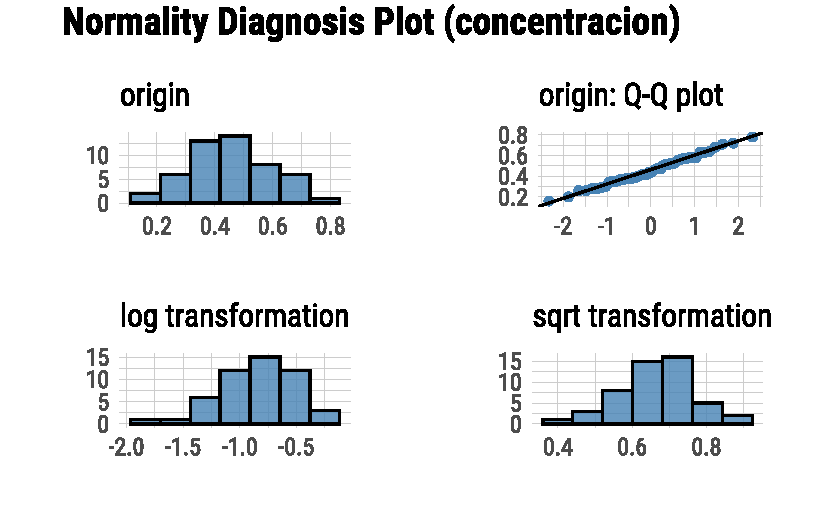
\includegraphics[width=0.85\linewidth,height=\textheight,keepaspectratio]{unidad_2/04_norm_het_files/figure-pdf/cod22-1.pdf}
\end{center}

Los puntos se desarrollan ``alrededor'' a la recta de normalidad.

Con estos dos elementos podemos confirmar que la distribución se
aproxima a la ``Normal'' y por lo tanto es confiable hacer uso de
métodos paramétricos.

Si bien con ayuda del Teorema del Límite Central (TCL) sabemos que si el
tamaño de la muestra es suficientemente grande, la distribución de la
media muestral (o del estadístico) tiende a una distribución normal,
independientemente de la forma que tengan los datos originales. En este
caso, la definición de ``grande'' depende de varios factores, pero
generalmente se considera que 30 es un buen umbral.

En la práctica, cuando trabajamos con variables continuas:

\begin{itemize}
\item
  Muestras pequeñas (\(n < 30\)): Si podemos asumir que la población
  original es aproximadamente normal, utilizamos la distribución \(t\)
  de Student con \(n-1\) grados de libertad. Esta distribución es más
  `ancha' en las colas, lo que penaliza nuestra incertidumbre por tener
  pocos datos.
\item
  Muestras grandes (\(n \ge 30\)): Por el TLC, la distribución del
  estadístico tiende a la normalidad (\(z\)). Sin embargo, dado que la
  distribución \(t\) converge a la \(z\) a medida que el tamaño de
  muestra aumenta, es una práctica estándar (y simplificadora) utilizar
  la distribución \(t\) en toda la escala.Por eso, funciones en R como
  \texttt{t.test()} se usan universalmente: para un \(n\) pequeño
  aplican la corrección necesaria, y para un \(n\) grande los resultados
  son virtualmente idénticos a los de una distribución \(z\).
\end{itemize}

Es una buena oportunidad para mencionar que el número 30 es una
convención histórica (una regla empírica). Actualmente, a veces con
\(n=30\) y datos muy sesgados, el TLC aún no ha ``actuado'' lo
suficiente y hay que recurrir a métodos no paramétricos donde obtenemos
IC más robustos y honestos que confiar ciegamente en la distribución
\(t\)``.

\subsection{Calculo de IC
paramétrica}\label{calculo-de-ic-paramuxe9trica}

Estamos frente al calculo de IC de una muestra de n = 50 (mayor a 30
observaciones) y que cumple con el supuesto de normalidad, por lo tanto
deciamos que podemos aplicar un método paramétrico basado en la
distribución \(t\) de Student.

Podríamos hacer las operaciones y cálculos individuales utilizando las
funciones que R tiene sobre esta distribución (familia TDist:
\texttt{qt()}, etc), pero la idea de este ejercicio es mostrarles la
forma operativa más sencilla de llevarlo a cabo.

\textbf{Función t.test()}

La función \texttt{t.test()}, incluída en el paquete stats de R base,
sirve apara ejecutar test de hipótesis de medias de una y dos
poblaciones (independientes o pareadas) pero además nos calcula
automáticamente el intervalo de confianza requerido, basado en la
distribución \(t\) de Student.

Para este ejemplo debemos utilizar como argumentos:

\begin{itemize}
\tightlist
\item
  la variable de interés que contiene los valores de la muestra
\item
  el nivel de confianza con el que necesitamos el IC
\end{itemize}

\begin{Shaded}
\begin{Highlighting}[]
\FunctionTok{t.test}\NormalTok{(}\AttributeTok{x =}\NormalTok{ bivalvos}\SpecialCharTok{$}\NormalTok{concentracion, }\AttributeTok{conf.level =} \FloatTok{0.95}\NormalTok{)}
\end{Highlighting}
\end{Shaded}

\begin{verbatim}

    One Sample t-test

data:  bivalvos$concentracion
t = 23.296, df = 49, p-value < 2.2e-16
alternative hypothesis: true mean is not equal to 0
95 percent confidence interval:
 0.4162995 0.4949005
sample estimates:
mean of x 
   0.4556 
\end{verbatim}

En la lista de resultados devuelta debemos observar los valores que
figuran debajo de ``95 percent confidence interval:''. En este caso, el
resultado es de una media de 0,4556 IC95\%: 0,4163-0,4949 partículas/g

Si cambiamos el argumento conf.level a 0.90 obtendremos el IC 90\%:

\begin{Shaded}
\begin{Highlighting}[]
\FunctionTok{t.test}\NormalTok{(}\AttributeTok{x =}\NormalTok{ bivalvos}\SpecialCharTok{$}\NormalTok{concentracion, }\AttributeTok{conf.level =} \FloatTok{0.90}\NormalTok{)}
\end{Highlighting}
\end{Shaded}

\begin{verbatim}

    One Sample t-test

data:  bivalvos$concentracion
t = 23.296, df = 49, p-value < 2.2e-16
alternative hypothesis: true mean is not equal to 0
90 percent confidence interval:
 0.4228123 0.4883877
sample estimates:
mean of x 
   0.4556 
\end{verbatim}

Este va de 0,4228 a 0,4884 partículas/g, lógicamente más estrecho que el
anterior porque redujimos el intervalo de confianza.

La redacción correcta sería \emph{``con un nivel de confianza del 90\%,
se estima que el verdadero valor de la media poblacional de la
concentración de microplásticos en bivalvos se encuentra entre 0,4228 y
0,4884 partículas/g.''}

Técnicamente las funciones estadísticas de R base devuelven generalmente
resultados en formato lista y reciben su entrada con formato vector o
bien sintaxis fórmula. Ese formato no cumple con ser ordenado como el
dataframe. Dado que la filosofía de trabajo del tidyverse (y por lo
tanto todos sus paquetes que pertenecen al ecosistema) tienen como
premisa recibir y devolver un dataframe, lo que permite usar tambien las
características tuberías, Kassambara (2026b) propuso el paquete
\textbf{rstatix}.

La idea central del paquete es ofrecer funciones que hacen lo mismo que
las de R base pero en lugar de devolver una lista de valores como
resultado lo haga mediante un dataframe.

Veamos su uso:

\begin{Shaded}
\begin{Highlighting}[]
\FunctionTok{library}\NormalTok{(rstatix)}

\NormalTok{bivalvos }\SpecialCharTok{|\textgreater{}}
  \FunctionTok{t\_test}\NormalTok{(concentracion }\SpecialCharTok{\textasciitilde{}} \DecValTok{1}\NormalTok{, }\AttributeTok{conf.level =} \FloatTok{0.95}\NormalTok{, }\AttributeTok{detailed =}\NormalTok{ T) }\SpecialCharTok{|\textgreater{}}
  \FunctionTok{select}\NormalTok{(estimate, conf.low, conf.high)}
\end{Highlighting}
\end{Shaded}

\begin{verbatim}
# A tibble: 1 x 3
  estimate conf.low conf.high
     <dbl>    <dbl>     <dbl>
1    0.456    0.416     0.495
\end{verbatim}

\subsection{\texorpdfstring{Construcción de
\textbf{umbral\_excedido}}{Construcción de umbral\_excedido}}\label{construcciuxf3n-de-umbral_excedido}

Debemos proceder ahora a construir la variable categórica
\textbf{umbral\_excedido} con valores Si y No en función del valor de
corte hipotético de 0,5.

Podemos hacerlo simplemente con el condicional \texttt{if\_else()}.

\begin{Shaded}
\begin{Highlighting}[]
\NormalTok{bivalvos }\OtherTok{\textless{}{-}}\NormalTok{ bivalvos }\SpecialCharTok{|\textgreater{}}
  \FunctionTok{mutate}\NormalTok{(}\AttributeTok{umbral\_excedido =} \FunctionTok{if\_else}\NormalTok{(concentracion }\SpecialCharTok{\textgreater{}} \FloatTok{0.5}\NormalTok{, }\StringTok{"Si"}\NormalTok{, }\StringTok{"No"}\NormalTok{))}

\NormalTok{bivalvos }\SpecialCharTok{|\textgreater{}}
  \FunctionTok{count}\NormalTok{(umbral\_excedido)}
\end{Highlighting}
\end{Shaded}

\begin{verbatim}
# A tibble: 2 x 2
  umbral_excedido     n
  <chr>           <int>
1 No                 31
2 Si                 19
\end{verbatim}

Observamos que 19 de los 50 bivalvos de nuestra muestra representa un
riesgo sanitario para los consumidores.

\begin{Shaded}
\begin{Highlighting}[]
\NormalTok{bivalvos }\SpecialCharTok{|\textgreater{}}
  \FunctionTok{count}\NormalTok{(umbral\_excedido) }\SpecialCharTok{|\textgreater{}}
  \FunctionTok{mutate}\NormalTok{(}\AttributeTok{porcentaje =}\NormalTok{ n }\SpecialCharTok{/} \FunctionTok{sum}\NormalTok{(n) }\SpecialCharTok{*} \DecValTok{100}\NormalTok{)}
\end{Highlighting}
\end{Shaded}

\begin{verbatim}
# A tibble: 2 x 3
  umbral_excedido     n porcentaje
  <chr>           <int>      <dbl>
1 No                 31         62
2 Si                 19         38
\end{verbatim}

Eso representa el 38\% de las observaciones que tenemos.

\subsection{IC 95\% de la proporción}\label{ic-95-de-la-proporciuxf3n}

En este punto queremos construir el intervalo de confianza del 95\% que
acompañe a la estimación puntual anterior.

Tenemos dos posibilidades que están implementadas en R base: la función
\texttt{prop.test()} o \texttt{binom.test()}.

\texttt{prop.test()} utiliza la aproximación de la distribución Normal
(puntuación \(z\)) a la distribución Binomial. Podríamos decir que es el
análogo categórico del \texttt{t.test(}). Los elementos necesarios son:
\textbf{x} número de éxitos y \textbf{n} que es tamaño de la muestra.

Se usa con muestras ``grandes'' (\(n > 30\)). Pero si en cambio el
tamaño de la muestra es pequeño, la proporción es muy cercana a 0 o a 1,
o quieres una precisión absoluta y no quieres depender de aproximaciones
matemáticas ejecutamos \texttt{binom.test()}.

La función aplica la prueba exacta de Clopper-Pearson, donde en
\textbf{x} definimos cuántos bivalvos superaron el umbral y en
\textbf{n} el tamaño total de la muestra.

Ejecutamos las dos posibilidades:

\begin{Shaded}
\begin{Highlighting}[]
\FunctionTok{prop.test}\NormalTok{(}\AttributeTok{x =} \DecValTok{19}\NormalTok{, }\AttributeTok{n =} \DecValTok{50}\NormalTok{)}
\end{Highlighting}
\end{Shaded}

\begin{verbatim}

    1-sample proportions test with continuity correction

data:  19 out of 50, null probability 0.5
X-squared = 2.42, df = 1, p-value = 0.1198
alternative hypothesis: true p is not equal to 0.5
95 percent confidence interval:
 0.2499804 0.5283672
sample estimates:
   p 
0.38 
\end{verbatim}

\begin{Shaded}
\begin{Highlighting}[]
\FunctionTok{binom.test}\NormalTok{(}\AttributeTok{x =} \DecValTok{19}\NormalTok{, }\AttributeTok{n =} \DecValTok{50}\NormalTok{)}
\end{Highlighting}
\end{Shaded}

\begin{verbatim}

    Exact binomial test

data:  19 and 50
number of successes = 19, number of trials = 50, p-value = 0.1189
alternative hypothesis: true probability of success is not equal to 0.5
95 percent confidence interval:
 0.2465011 0.5282508
sample estimates:
probability of success 
                  0.38 
\end{verbatim}

Los resultados son muy similares, dado que cumplimos con los supuestos
necesarios para usar la aproximación del test de proporciones.

Entonces podemos decir con un nivel de confianza del 95\%, que estimamos
que la proporción poblacional de bivalvos que exceden el límite de
seguridad sanitaria se encuentra entre 0,25 y 0,53.

Las dos funciones estan representadas en \textbf{rstatix}, con
\texttt{prop\_test()} y \texttt{binom\_test()} respectivamente.

Apredimos con este ejercicio que el lenguaje R siempre ofrece múltiples
caminos, pero nuestro criterio es el que decide cuál usar y reportar.

Wickham et~al. (2019)

\section{Referencias}\label{referencias-7}

\chapter{Selección de la muestra}\label{selecciuxf3n-de-la-muestra}

\section{Introducción}\label{introducciuxf3n-7}

Toda investigación epidemiológica requiere, en principio, la selección
de una muestra representativa de la población objeto de estudio. Esto
implica:

\begin{itemize}
\item
  Determinar el tamaño de la muestra.
\item
  Definir cómo se seleccionarán los sujetos (es decir, las unidades de
  análisis).
\item
  Calcular la incertidumbre que introduce este proceso de muestreo en
  nuestras estimaciones.
\end{itemize}

El tamaño de la muestra se establece en la fase de diseño del estudio,
habitualmente cuando se redacta el protocolo de investigación. Es
importante considerar que este tamaño es, en cierto sentido, orientador,
ya que su cálculo depende de factores que en ocasiones pueden ser
subjetivos o estar limitados por la información previa disponible.
Además, las exigencias varían según el objetivo del estudio. Por
ejemplo:

\begin{itemize}
\item
  En un estudio transversal, donde se estima una prevalencia, se puede
  aceptar una precisión menor.
\item
  En un estudio experimental, donde se compara la eficacia de un fármaco
  frente a un placebo, el tamaño de la muestra debe ser suficiente para
  detectar una ``diferencia significativa'' entre los grupos.
\end{itemize}

Cuando el objetivo de la investigación incluye la estimación de un
intervalo de confianza (IC) para alguna variable, se busca que dicho IC
tenga alta confiabilidad y sea lo más estrecho posible.

En el caso de los estudios de corte transversal, que se orientan a
estimar una proporción, se formulan preguntas como:\\
--- ¿Cuál es la prevalencia, proporción o porcentaje del fenómeno en
estudio?

Al tomar una muestra para estimar lo que sucede en la realidad, debemos
aceptar que la medición obtenida reflejará la situación poblacional,
pero siempre con cierto grado de variabilidad (o error). La
\textbf{precisión} es ese grado de variabilidad aceptable y se expresa a
través de los intervalos de confianza, que definen los límites inferior
y superior dentro de los cuales se espera encontrar el verdadero valor
del parámetro.

\section{Cálculo del tamaño
muestral}\label{cuxe1lculo-del-tamauxf1o-muestral}

Como se mencionó anteriormente, se requiere conocer algunos datos para
el cálculo del tamaño de muestra requerido, entre los que destacan:

\begin{itemize}
\item
  \textbf{La proporción esperada del evento:} Aunque resulte paradójico,
  ya que es el parámetro que se desea estimar, el investigador suele
  contar con información previa que permite delimitar sus posibles
  valores. Si no fuera el caso, se utiliza el peor escenario, es decir,
  una proporción del 50\%, ya que este valor maximiza el producto
  \(p(1-p)\) y, por ende, exige el mayor tamaño muestral. De esta forma,
  muchas veces se recurre a esto para tener al menos una idea del
  ``límite superior'' que estaríamos manejando.
\item
  \textbf{El nivel de confianza deseado:} Habitualmente se emplea un
  95\% (lo que equivale a un \(\alpha\) de 0.05). Este valor indica la
  probabilidad de que el intervalo calculado contenga el parámetro
  poblacional verdadero. A mayor nivel de confianza (es decir, menor
  \(\alpha\)), mayor es el coeficiente de confiabilidad y, por ende,
  mayor el tamaño muestral requerido.
\item
  \textbf{La precisión (}\(\delta\)\textbf{) deseada:} Se refiere a la
  amplitud aceptable del intervalo de confianza. Cuanta más precisión se
  exija (es decir, un intervalo más estrecho), mayor será el tamaño de
  la muestra necesario.
\end{itemize}

La fórmula para el cálculo es la siguiente:

\[
N = \frac{p.q.(Z\alpha)^2}{\delta^2}
\]

Donde: - \(N\) es el tamaño muestra requerido. - \(p\) es la proporción
esperada de sujetos portadores del evento. - \(q = 1 – p\) es la
proporción complementaria (sujetos que no tienen la variable en
estudio). - \(\delta\) es la precisión o magnitud de error aceptable. -
\(Z\alpha\) es el valor crítico de la distribución normal asociado al
nivel de significancia. Se obtiene de tablas de distribución normal de
probabilidades y habitualmente se utiliza un valor \(\alpha\) de 0.05,
al que le corresponde un valor \(Z\) de 1.96

Cuando se conoce el tamaño de la población, es necesario aplicar una
corrección por población finita:

\[
N =\frac{n^1}{1+\frac{n^1}{Población}}
\]

donde \(n^1\) es el \(N\) calculado con la ecuación anterior.

Es fundamental entender que el tamaño de la muestra dependerá de \(p\)
de \(\alpha\) y de la precisión deseada, más que de la complejidad de la
fórmula en sí. Existen numerosos softwares que calculan tamaños de
muestra. Algunos están especializados en esta tarea (por ejemplo,
\textbf{EpiDat}, \textbf{EpiInfo}, \textbf{OpenEp}i), mientras que otros
lo incluyen como una opción dentro de un paquete más amplio de análisis.
En el lenguaje R, funciones como \texttt{power.prop.test()} (para
comparación de proporciones) y \texttt{power.t.test()} (para pruebas de
medias basadas en la distribución \(t\) de Student) están incluidas en
el paquete \texttt{stats}. Otros paquetes útiles incluyen
\texttt{samplingbook} (Manitz et~al. 2021), \texttt{samplesize},
\texttt{pwr} (Champely 2020) y \texttt{epiR} (Stevenson y Sergeant
2026).

A continuación, se presenta un ejemplo práctico utilizando la función
\texttt{sample.size.prop()} del paquete \texttt{samplingbook}.
Supongamos que queremos estimar la prevalencia de diabetes en una ciudad
de 600,000 habitantes, donde estudios previos sugieren una prevalencia
cercana al 10.2\%. El objetivo es determinar el tamaño de la muestra en
un muestreo aleatorio simple.

Comenzamos cargando el paquete requerido:

\begin{Shaded}
\begin{Highlighting}[]
\FunctionTok{library}\NormalTok{(samplingbook)}
\end{Highlighting}
\end{Shaded}

Calculamos el tamaño muestral en base a los siguientes argumentos:

\begin{itemize}
\tightlist
\item
  \texttt{e}: número positivo que especifica la precisión que es la
  mitad del ancho del intervalo de confianza
\item
  \texttt{p:} proporción esperada de eventos con dominio entre los
  valores 0 y 1.
\item
  \texttt{N}: número entero positivo para el tamaño de la población. El
  valor predeterminado es \texttt{Inf}, lo que significa que los
  cálculos se realizan sin \emph{corrección de población finita}.
\item
  \texttt{level}: nivel de confianza para los intervalos de confianza.
  El valor predeterminado es 95\%.
\end{itemize}

\begin{Shaded}
\begin{Highlighting}[]
\FunctionTok{sample.size.prop}\NormalTok{(}\AttributeTok{e =} \FloatTok{0.02}\NormalTok{, }\AttributeTok{P =} \FloatTok{0.102}\NormalTok{, }\AttributeTok{N =} \DecValTok{600000}\NormalTok{, }\AttributeTok{level =} \FloatTok{0.95}\NormalTok{)}
\end{Highlighting}
\end{Shaded}

\begin{verbatim}

sample.size.prop object: Sample size for proportion estimate
With finite population correction: N=6e+05, precision e=0.02 and expected proportion P=0.102

Sample size needed: 879
\end{verbatim}

El resultado, tras aplicar la corrección por población finita, indica
que se requieren 879 sujetos en la muestra. Por simplicidad, es habitual
considerar infinita a la población objetivo, ya que hacerlo así minimiza
los riesgos estadísticos:

\begin{Shaded}
\begin{Highlighting}[]
\FunctionTok{sample.size.prop}\NormalTok{(}\AttributeTok{e =} \FloatTok{0.02}\NormalTok{, }\AttributeTok{P =} \FloatTok{0.102}\NormalTok{, }\AttributeTok{N =} \ConstantTok{Inf}\NormalTok{, }\AttributeTok{level =} \FloatTok{0.95}\NormalTok{)}
\end{Highlighting}
\end{Shaded}

\begin{verbatim}

sample.size.prop object: Sample size for proportion estimate
Without finite population correction: N=Inf, precision e=0.02 and expected proportion P=0.102

Sample size needed: 880
\end{verbatim}

Si se considera una población infinita, el tamaño muestral calculado es
de 880 personas, apenas una unidad más, lo que demuestra que el ajuste
por población finita en este caso es mínimo. En cambio, si no se conoce
o no se confía en el valor de prevalencia y se opta por el peor
escenario (\(p = 0.5\)):

\begin{Shaded}
\begin{Highlighting}[]
\FunctionTok{sample.size.prop}\NormalTok{(}\AttributeTok{e =} \FloatTok{0.02}\NormalTok{, }\AttributeTok{P =} \FloatTok{0.5}\NormalTok{, }\AttributeTok{N =} \DecValTok{600000}\NormalTok{, }\AttributeTok{level =} \FloatTok{0.95}\NormalTok{)}
\end{Highlighting}
\end{Shaded}

\begin{verbatim}

sample.size.prop object: Sample size for proportion estimate
With finite population correction: N=6e+05, precision e=0.02 and expected proportion P=0.5

Sample size needed: 2392
\end{verbatim}

En este caso, el tamaño muestral aumenta considerablemente hasta 2392
unidades, lo que refleja un enfoque más conservador.

Además del cálculo del tamaño muestral, es esencial planificar la forma
en que se seleccionarán los individuos. En estudios de corte transversal
se debe realizar un muestreo probabilístico, ya que la técnica de
muestreo influirá en los factores de expansión necesarios para
generalizar los resultados a la población. Aunque el proceso de muestreo
no se detalla en este curso, es vital considerarlo para garantizar la
validez externa de la investigación.

\section{Conceptos generales sobre
muestreo}\label{conceptos-generales-sobre-muestreo}

Un muestreo se considera \textbf{probabilístico} cuando se cumplen dos
condiciones fundamentales:

\begin{itemize}
\item
  Es posible conocer de antemano la probabilidad de selección que tiene
  cada elemento de la población.
\item
  Esta probabilidad es mayor que cero para todos los elementos.
\end{itemize}

Solo con un muestreo probabilístico se puede medir el grado de precisión
de las estimaciones realizadas, ya que se conocen las probabilidades de
inclusión. Algunos de los métodos más usados son: Muestreo aleatorio
simple, muestreo sistemático en fases, Muestreo aleatorio estratificado,
muestreo por conglomerados, etc.

\subsection{Muestreo aleatorio simple
(MAS)}\label{muestreo-aleatorio-simple-mas}

En el MAS, cada elemento de la población tiene la misma probabilidad de
ser seleccionado (es decir, es un método \textbf{equiprobabilístico}).
La probabilidad de inclusión se expresa como:

\[
P = \frac{n}{N}
\]

donde:

\begin{itemize}
\item
  \(n\) es el tamaño de la muestra,
\item
  \(N\) es el tamaño de la población.
\end{itemize}

Este método requiere contar con un listado completo de la población y se
utiliza principalmente en poblaciones cerradas (por ejemplo, escuelas,
cárceles, hospitales o muestras de laboratorio), donde los elementos
pueden identificarse y numerarse fácilmente.

\subsection{Muestreo sistemático (MS)}\label{muestreo-sistemuxe1tico-ms}

El muestreo sistemático es un procedimiento alternativo al MAS, adecuado
para la selección de muestras equiprobabilísticas de poblaciones
organizadas según algún orden conocido. Sus ventajas incluyen no
requerir necesariamente un listado completo de todas las unidades, lo
que resulta útil, por ejemplo, para seleccionar a los usuarios que
llegan a un servicio hospitalario durante un período determinado.

El procedimiento consiste en:

\begin{enumerate}
\def\labelenumi{\arabic{enumi}.}
\item
  Asignar a cada elemento de la población un número del 1 a \(N\).
\item
  Calcular el intervalo de selección:
\end{enumerate}

\[
k = \frac{N}{n}
\]

\begin{enumerate}
\def\labelenumi{\arabic{enumi}.}
\setcounter{enumi}{2}
\item
  Seleccionar aleatoriamente un número \(r\) entre 1 y \(k\).
\item
  Elegir los elementos que ocupan las posiciones:
  \(r, r+k, r + 2k,...\), es decir, la secuencia \(r, r+jk\) con
  \(j = 0, 1, 2, \dots\).
\end{enumerate}

La probabilidad de ser seleccionado es igual que en el MAS

\[
P = \frac{n}{N} 
\]

\subsection{Muestreo aleatorio estratificado
(MAE)}\label{muestreo-aleatorio-estratificado-mae}

Este método se emplea cuando la población puede dividirse en subgrupos o
\textbf{estratos} que difieren en las características de interés (por
ejemplo, edad, sexo o nivel socioeconómico). La idea es asegurar que
cada estrato esté representado en la muestra. El proceso habitual
consiste en:

\begin{itemize}
\item
  Elaborar listas separadas para cada estrato.
\item
  Seleccionar una submuestra de cada uno de ellos.
\end{itemize}

La probabilidad de selección en cada estrato es:

\[
P \ estrato = \frac{n \ estrato}{N \ estrato} 
\]

Si se aplica un muestreo proporcional, el tamaño de la muestra en cada
estrato se calcula como:

\[
n \ estrato = n\frac{N \ estrato}{N} 
\]

El objetivo es obtener una muestra cuya variabilidad interna se asemeje
a la de la población, logrando que los estratos sean internamente
homogéneos y heterogéneos entre sí.

\subsection{Muestreo por conglomerados
monoetápico}\label{muestreo-por-conglomerados-monoetuxe1pico}

El muestreo por conglomerados es ideal cuando la población es difícil de
delimitar o está muy dispersa. Se divide la población en
\textbf{conglomerados} (o grupos) que actúan como unidades de primera
etapa (UPE) y no deben solaparse.

La población se divide en grupos (por ejemplo, áreas geográficas,
instituciones o servicios). Se selecciona una muestra de \(n\)
conglomerados y se incluyen \textbf{todos} las unidades de análisis de
los conglomerados seleccionados. El tamaño del conglomerado se refiere
al número de unidades elementales que contiene, pudiendo ser de igual o
distinto tamaño. Los conglomerados deberían ser lo más heterogéneos
dentro de ellos y lo más homogéneos entre ellos.

\subsection{Muestreo por conglomerados
bietápico}\label{muestreo-por-conglomerados-bietuxe1pico}

Se utiliza cuando existe gran variabilidad en el tamaño de los
conglomerados o la población es muy grande. En este caso, después de
dividir la población en conglomerados y seleccionar algunos de ellos
como UPE, se realiza una subselección (muestreo secundario) de los
elementos dentro de los conglomerados elegidos.

Existen más posibilidades, que no abordaremos aquí, pero sí nos
detendremos en discutir qué implicaciones tiene el muestreo en el
proceso de estimación.

\subsection{Implicaciones en la Estimación y
Ponderación}\label{implicaciones-en-la-estimaciuxf3n-y-ponderaciuxf3n}

En métodos equiprobabilísticos (como el MAS o el MS), cada elemento
tiene la misma probabilidad de selección. Sin embargo, en diseños
muestrales más complejos (como el muestreo estratificado o por
conglomerados), las probabilidades de selección pueden variar entre
individuos.

En estos casos, la probabilidad total de selección de un individuo es el
producto de las probabilidades de selección en cada etapa del muestreo.
Una vez conocida esta probabilidad, se calcula el peso (o \textbf{factor
de expansión}) como su inverso. Este peso se interpreta como el número
de individuos en la población que representa cada individuo de la
muestra.

\begin{quote}
El factor de expansión se interpreta como \emph{la cantidad de personas
en la población, que representa una persona en la muestra}.
\end{quote}

El factor de expansión se utiliza para extrapolar los resultados
obtenidos en la muestra a la población total. Por ejemplo, para estimar
un total poblacional para una variable, se pondera el valor medido en
cada individuo por su factor de expansión y se suman dichos valores.

\section{Ejemplo práctico}\label{ejemplo-pruxe1ctico}

Supongamos que queremos estimar la prevalencia de sobrepeso/obesidad en
estudiantes de enseñanza media de una localidad. Se tiene la siguiente
información:

\begin{itemize}
\item
  \textbf{Población total de alumnos:} 966
\item
  \textbf{Número de escuelas (conglomerados):} 21
\item
  \textbf{Tamaño de la muestra global (ya calculado):} 120 alumnos
\end{itemize}

Si se realizara un \textbf{muestreo aleatorio simple (MAS)}, se
necesitaría disponer del listado completo de los 966 alumnos y, mediante
un sorteo, seleccionar 120 individuos. En ese caso, la probabilidad de
selección para cada alumno sería:

\[
P = \frac{n}{N} = \frac{120}{966}=0,124
\]

Supongamos ahora que decide realizar un muestreo por conglomerados
biétapico. Cada escuela se considera un conglomerado; se seleccionan 10
de las 21 escuelas por MAS y, dentro de cada escuela seleccionada, se
elige una submuestra de estudiantes también mediante MAS. Se decide que
el número de estudiantes elegidos en cada conglomerado sea igual para
todos.

Los datos globales quedan de la siguiente forma:

\begin{table}
\fontsize{12.0pt}{14.0pt}\selectfont
\begin{tabular*}{\linewidth}{@{\extracolsep{\fill}}lrr}
\toprule
  & Población & Muestra \\ 
\midrule\addlinespace[2.5pt]
Tamaño total & 966 & 120 \\ 
Número de conglomerados & 21 & 10 \\ 
\bottomrule
\end{tabular*}
\end{table}

La decisión de cuántos conglomerados forman parte de la muestra, es una
decisión del investigador: a veces puede ser necesario fijar un número,
a veces puede ser más conveniente fijar el tamaño de la muestra en cada
conglomerado. Por otra parte, puede que decidamos que el número de
sujetos seleccionados en cada conglomerado sea igual para todos; que sea
una fracción fija o algo a definir.

Dentro de los conglomerados seleccionados, se obtiene la siguiente
distribución (en este ejemplo, la suma de los tamaños de los
conglomerados seleccionados es 480 y en cada uno se eligen 12 alumnos):

\begin{table}
\fontsize{12.0pt}{14.0pt}\selectfont
\begin{tabular*}{\linewidth}{@{\extracolsep{\fill}}lrr}
\toprule
Conglomerado & Tamaño & Muestra \\ 
\midrule\addlinespace[2.5pt]
5.1 & 48 & 12 \\ 
1.3 & 28 & 12 \\ 
2.3 & 64 & 12 \\ 
2.2 & 43 & 12 \\ 
3.1 & 37 & 12 \\ 
5.3 & 86 & 12 \\ 
1.4 & 37 & 12 \\ 
3.3 & 56 & 12 \\ 
2.4 & 48 & 12 \\ 
1.5 & 33 & 12 \\ 
Total & 480 & 120 \\ 
\bottomrule
\end{tabular*}
\end{table}

\subsection{Cálculo de las Probabilidades de Selección y
Ponderaciones}\label{cuxe1lculo-de-las-probabilidades-de-selecciuxf3n-y-ponderaciones}

Para que un individuo sea seleccionado en este diseño, debe ocurrir
primero que su conglomerado sea escogido y, posteriormente, que él sea
seleccionado dentro de ese conglomerado. Si asumimos que:

\begin{quote}
\emph{``Dos sucesos son independientes si la probabilidad de que ocurran
ambos simultáneamente es igual al producto de las probabilidades de que
ocurra cada uno de ellos''}.
\end{quote}

La probabilidad total de selección es el producto de:

\begin{enumerate}
\def\labelenumi{\arabic{enumi}.}
\tightlist
\item
  La probabilidad de que el conglomerado sea seleccionado:
\end{enumerate}

\[
P_{conglomerado} = \frac{10}{21}
\]

\begin{enumerate}
\def\labelenumi{\arabic{enumi}.}
\setcounter{enumi}{1}
\tightlist
\item
  La probabilidad de que un individuo sea seleccionado dentro de su
  conglomerado:
\end{enumerate}

\[
P_{dentro} = \frac{N°~alumnos~en~la~muestra~del~conglomerado}{Tamaño~del~conglomerado}
\]

Para los individuos del conglomerado 5.1; la probabilidad de selección
será:

\[
P_{5.1} = \frac{10}{21}*\frac{12}{48} \approx 0,1190 \quad (11.9\%)
\]

La ponderación o \textbf{factor de expansión} se obtiene como el inverso
de la probabilidad de selección:

\[
w = \frac{1}{P}
\]

Es decir:

\[
w_{5.1} = \frac{1}{1.190} \approx 8.4
\]

Esto significa que cada alumno seleccionado del conglomerado 5.1
representa aproximadamente a 8 alumnos de la población.

Si se realizan los cálculos para cada uno de los conglomerados, se
obtiene la siguiente tabla:

\begin{table}
\fontsize{12.0pt}{14.0pt}\selectfont
\begin{tabular*}{\linewidth}{@{\extracolsep{\fill}}rrr}
\toprule
Conglomerado & Probabilidad & Ponderación \\ 
\midrule\addlinespace[2.5pt]
5.1 & 11.90 & 8.40 \\ 
1.3 & 20.41 & 4.90 \\ 
2.3 & 8.93 & 11.20 \\ 
2.2 & 13.29 & 7.53 \\ 
3.1 & 15.44 & 6.48 \\ 
5.3 & 6.65 & 15.05 \\ 
1.4 & 15.44 & 6.48 \\ 
3.3 & 10.20 & 9.80 \\ 
2.4 & 11.90 & 8.40 \\ 
1.5 & 17.32 & 5.78 \\ 
\bottomrule
\end{tabular*}
\end{table}

Cada individuo seleccionado en el estudio tiene una probabilidad de
inclusión que depende tanto de la probabilidad de que su escuela
(conglomerado) sea seleccionada como de la probabilidad de que él sea
elegido dentro de su escuela. La ponderación resultante (el inverso de
esta probabilidad) se utiliza para ``expandir'' el resultado del
estudio, de manera que cada alumno en la muestra represente a un número
determinado de alumnos en la población total.

Por ejemplo, en el conglomerado 5.1, cada alumno seleccionado representa
aproximadamente a 8 alumnos de la población. De este modo, al calcular
la prevalencia de sobrepeso/obesidad en la muestra, se aplican estos
factores de expansión para obtener estimaciones que sean representativas
de los 966 alumnos de la localidad.

Este proceso es fundamental en estudios basados en muestreos complejos,
ya que permite corregir posibles diferencias en las probabilidades de
selección y garantizar que las estimaciones sean válidas y precisas para
toda la población.

Hernández-Ávila (2011)

Daniel (2002)

Rodríguez y Mendivelso (2018)

Ríus Díaz et~al. (2012)

Triola (2018)

Norman, GR y Streiner, DL (1996)

Rodríguez et~al. (2003)

\emph{{EPIDAT} 4.2 - {Consellería} de {Sanidade} - {Servizo} {Galego} de
{Saúde}} (s.~f.)

Elm et~al. (2008)

Schulz et~al. (2010)

Álvarez Cáceres (2007)

Glantz, S (2006)

Field et~al. (2014)

\section{Referencias}\label{referencias-8}

\chapter{Funciones condicionales en
R}\label{funciones-condicionales-en-r}

\section{Introducción}\label{introducciuxf3n-8}

Continuamos incorporando funciones útiles para el manejo de datos,
enfocándonos en la creación de nuevas variables y en la transformación
de variables cuantitativas a variables categóricas, ya sean nominales u
ordinales.

Algunas de estas operaciones serán necesarias para alcanzar los
objetivos del trabajo práctico grupal de esta unidad, y seguramente
también se utilizarán en las unidades siguientes.

Como vimos dentro del universo \texttt{tidyverse}, para crear nuevas
variables a partir de cálculos utilizamos la función-verbo
\texttt{mutate()}:

\begin{Shaded}
\begin{Highlighting}[]
\NormalTok{datos }\OtherTok{\textless{}{-}}\NormalTok{ datos }\SpecialCharTok{|\textgreater{}}
  \FunctionTok{mutate}\NormalTok{(}\AttributeTok{variable\_nueva =} \FunctionTok{funcion}\NormalTok{(var1))}
\end{Highlighting}
\end{Shaded}

Frecuentemente necesitaremos agrupar, resumir o \textbf{discretizar
variables continuas}, dividiendo su rango en categorías que pueden ser
\textbf{dicotómicas} o \textbf{politómicas}, según los objetivos del
análisis.

\section{\texorpdfstring{Condicional simple:
\texttt{if\_else()}}{Condicional simple: if\_else()}}\label{condicional-simple-if_else}

Para obtener salidas dicotómicas, podemos usar la función condicional
\texttt{if\_else()} del paquete \texttt{dplyr}. Esta función es una
versión simplificada y segura del clásico condicional \texttt{if} que
existe en la mayoría de los lenguajes de programación, así como en hojas
de cálculo como \emph{Microsoft Excel®} y \emph{Google Sheets®}, entre
otras.

Supongamos que tenemos un dataframe llamado \texttt{datos}, con una
variable cuantitativa denominada \texttt{var1}:

\begin{Shaded}
\begin{Highlighting}[]
\CommentTok{\# Cargar tidyverse}
\FunctionTok{library}\NormalTok{(tidyverse)}

\CommentTok{\# Datos ejemplo}
\FunctionTok{set.seed}\NormalTok{(}\DecValTok{123}\NormalTok{)}

\NormalTok{datos }\OtherTok{\textless{}{-}} \FunctionTok{tibble}\NormalTok{(}
  \AttributeTok{var1 =} \FunctionTok{sample}\NormalTok{(}\DecValTok{1}\SpecialCharTok{:}\DecValTok{90}\NormalTok{, }\AttributeTok{size =} \DecValTok{50}\NormalTok{, }\AttributeTok{replace =} \ConstantTok{TRUE}\NormalTok{)}
\NormalTok{)}
\end{Highlighting}
\end{Shaded}

Queremos crear una variable cualitativa dentro de \texttt{datos},
llamada \texttt{variable\_nueva}, cuyos valores estén dados por el
cumplimiento de alguna condición de \texttt{var1}. Por ejemplo, si los
valores de \texttt{var1} son mayores a 10, entonces
\texttt{variable\_nueva}, tomará el valor \texttt{“mayor\ a\ 10”}, en
caso contrario, tomará el valor \texttt{“menor\ o\ igual\ a\ 10”}:

\begin{Shaded}
\begin{Highlighting}[]
\CommentTok{\# Crear variable\_nueva}
\NormalTok{datos }\OtherTok{\textless{}{-}}\NormalTok{ datos }\SpecialCharTok{|\textgreater{}}
  \FunctionTok{mutate}\NormalTok{(}
    \AttributeTok{variable\_nueva =} \FunctionTok{if\_else}\NormalTok{(}
      \AttributeTok{condition =}\NormalTok{ var1 }\SpecialCharTok{\textgreater{}} \DecValTok{10}\NormalTok{,}
      \AttributeTok{true =} \StringTok{"mayor a 10"}\NormalTok{,}
      \AttributeTok{false =} \StringTok{"menor o igual a 10"}
\NormalTok{    )}
\NormalTok{  )}

\CommentTok{\# Explorar variable\_nueva}
\FunctionTok{tabyl}\NormalTok{(datos, variable\_nueva)}
\end{Highlighting}
\end{Shaded}

\begin{verbatim}
     variable_nueva  n percent
         mayor a 10 44    0.88
 menor o igual a 10  6    0.12
\end{verbatim}

La función \texttt{if\_else()} tiene tres argumentos obligatorios:

\begin{itemize}
\item
  \texttt{condition}: la condición a evaluar.
\item
  \texttt{true}: valor que tomará la nueva variable si se cumple la
  condición.
\item
  \texttt{false}: valor que tomará la nueva variable si no se cumple la
  condición.
\end{itemize}

Este proceso se conoce como \textbf{dicotomización} de una variable, ya
que el resultado posible consta de solo dos categorías.

Los valores de salida pueden ser de distintos tipos (carácter, numérico
o lógico). Sin embargo, cuando discretizamos una variable cuantitativa,
habitualmente generamos una variable cualitativa de tipo
\textbf{ordinal}, con categorías expresadas como texto (tipo
\texttt{character}).

Ahora bien, al ser ordinal estas categorías de la
\texttt{variable\_nueva} deben ``ordenarse'' en la forma de los valores
de la variable, pero el lenguaje R no sabe con que estamos trabajando y
respeta siempre el ordenamiento alfanumérico. Por lo tanto, en este
ejemplo las categorías se van a estar ordenando al reves del orden
numérico natural (de menor a mayor).

La categoría \texttt{"mayor\ a\ 10”} se ordena alfabéticamente antes de
\texttt{“menor\ o\ igual\ a\ 10”}, porque luego del empate de las letras
\texttt{m}, le siguen la \texttt{a} en el primer caso y la \texttt{e} en
el segundo.

Para ordenar estas categorías debemos transformar la variable de
\texttt{character} a \texttt{factor}. Esto se puede hacer en un solo
paso dentro del \texttt{mutate()}:

\begin{Shaded}
\begin{Highlighting}[]
\NormalTok{datos }\OtherTok{\textless{}{-}}\NormalTok{ datos }\SpecialCharTok{|\textgreater{}}
  \FunctionTok{mutate}\NormalTok{(}
    \AttributeTok{variable\_nueva =} \FunctionTok{if\_else}\NormalTok{(}
      \AttributeTok{condition =}\NormalTok{ var1 }\SpecialCharTok{\textgreater{}} \DecValTok{10}\NormalTok{,}
      \AttributeTok{true =} \StringTok{"mayor a 10"}\NormalTok{,}
      \AttributeTok{false =} \StringTok{"menor o igual a 10"}
\NormalTok{    ),}

    \AttributeTok{variable\_nueva =} \FunctionTok{factor}\NormalTok{(}
\NormalTok{      variable\_nueva,}
      \AttributeTok{levels =} \FunctionTok{c}\NormalTok{(}\StringTok{"menor o igual a 10"}\NormalTok{, }\StringTok{"mayor a 10"}\NormalTok{)}
\NormalTok{    )}
\NormalTok{  )}

\CommentTok{\# Explorar variable\_nueva}
\FunctionTok{tabyl}\NormalTok{(datos, variable\_nueva)}
\end{Highlighting}
\end{Shaded}

\begin{verbatim}
     variable_nueva  n percent
 menor o igual a 10  6    0.12
         mayor a 10 44    0.88
\end{verbatim}

Otra forma más artesanal, igualmente válido, es ``forzar'' el
ordenamiento con las categorías así:

\begin{Shaded}
\begin{Highlighting}[]
\NormalTok{datos }\OtherTok{\textless{}{-}}\NormalTok{ datos }\SpecialCharTok{|\textgreater{}}
  \FunctionTok{mutate}\NormalTok{(}
    \AttributeTok{variable\_nueva =} \FunctionTok{if\_else}\NormalTok{(}
      \AttributeTok{condition =}\NormalTok{ var1 }\SpecialCharTok{\textgreater{}} \DecValTok{10}\NormalTok{,}
      \AttributeTok{true =} \StringTok{"2.mayor a 10"}\NormalTok{,}
      \AttributeTok{false =} \StringTok{"1.menor o igual a 10"}
\NormalTok{    )}
\NormalTok{  )}

\CommentTok{\# Explorar variable\_nueva}
\FunctionTok{tabyl}\NormalTok{(datos, variable\_nueva)}
\end{Highlighting}
\end{Shaded}

\begin{verbatim}
       variable_nueva  n percent
 1.menor o igual a 10  6    0.12
         2.mayor a 10 44    0.88
\end{verbatim}

Aquí agregamos números iniciales a las etiquetas de las categorías para
darle el orden que deseamos, sin necesidad de convertir a factor.

\subsection{\texorpdfstring{Función
\textbf{\texttt{cut\_interval()}}}{Función cut\_interval()}}\label{funciuxf3n-cut_interval}

El ecosistema \texttt{tidyverse} ofrece la función
\texttt{cut\_interval()} para la creación de intervalos regulares.

Es una adaptación de la función \texttt{cut()} de R base para \emph{tidy
data} y sus argumentos son similares. Volviendo al ejemplo anterior:

\begin{Shaded}
\begin{Highlighting}[]
\NormalTok{datos }\OtherTok{\textless{}{-}}\NormalTok{ datos }\SpecialCharTok{|\textgreater{}}
  \FunctionTok{mutate}\NormalTok{(}
    \AttributeTok{grupo\_var =} \FunctionTok{cut\_interval}\NormalTok{(}
      \AttributeTok{x =}\NormalTok{ var1,}
      \AttributeTok{length =} \DecValTok{10}\NormalTok{,}
      \AttributeTok{right =} \ConstantTok{TRUE}\NormalTok{,}
      \AttributeTok{ordered\_result =} \ConstantTok{TRUE}
\NormalTok{    )}
\NormalTok{  )}

\CommentTok{\# Explora grupo\_var}
\FunctionTok{tabyl}\NormalTok{(datos, grupo\_var)}
\end{Highlighting}
\end{Shaded}

\begin{verbatim}
 grupo_var n percent
    [0,10] 6    0.12
   (10,20] 4    0.08
   (20,30] 7    0.14
   (30,40] 6    0.12
   (40,50] 6    0.12
   (50,60] 5    0.10
   (60,70] 4    0.08
   (70,80] 7    0.14
   (80,90] 5    0.10
\end{verbatim}

Los argumentos función son:

\begin{itemize}
\item
  \texttt{x}: conjunto de datos numéricos de entrada (obligatorio).
\item
  \texttt{length}: longitud de cada intervalo regular (obligatorio).
\item
  \texttt{n}: cantidad de intervalos a crear (obligatorio, omitir si se
  definió \texttt{length}).
\item
  \texttt{right}: indica si los intervalos son cerrados a la derecha o
  viceversa (valor por defecto \texttt{TRUE}, intervalos cerrados a la
  derecha).
\item
  \texttt{labels}: etiquetas de los intervalos automáticas o numéricas
  (por defecto intervalos matemáticos).
\item
  \texttt{ordered\_result}: determina si el resultado es un factor
  ordenado. Por defecto vale \texttt{FALSE} (la salida es tipo
  carácter).
\end{itemize}

No es necesario definir los argumentos opcionales siempre y cuando los
valores por defecto sirvan para nuestra tarea.

\section{\texorpdfstring{Función
\texttt{case\_when()}}{Función case\_when()}}\label{funciuxf3n-case_when}

Cuando las condiciones no son simples, es decir, el resultado no es
dicotómico y además los intervalos son irregulares, utilizamos la
función \texttt{case\_when()} que es una vectorización de la función
\texttt{if\_else()}.

Supongamos que queremos agrupar la variable cuantitativa de números
enteros (\texttt{var1}) en tres grupos irregulares:

\begin{Shaded}
\begin{Highlighting}[]
\NormalTok{datos }\OtherTok{\textless{}{-}}\NormalTok{ datos }\SpecialCharTok{|\textgreater{}}
  \FunctionTok{mutate}\NormalTok{(}
    \AttributeTok{grupo\_var =} \FunctionTok{case\_when}\NormalTok{(}
\NormalTok{      var1 }\SpecialCharTok{\%in\%} \FunctionTok{c}\NormalTok{(}\DecValTok{0}\SpecialCharTok{:}\DecValTok{24}\NormalTok{) }\SpecialCharTok{\textasciitilde{}} \StringTok{"Grupo 1"}\NormalTok{,}
\NormalTok{      var1 }\SpecialCharTok{\%in\%} \FunctionTok{c}\NormalTok{(}\DecValTok{25}\SpecialCharTok{:}\DecValTok{64}\NormalTok{) }\SpecialCharTok{\textasciitilde{}} \StringTok{"Grupo 2"}\NormalTok{,}
\NormalTok{      var1 }\SpecialCharTok{\textgreater{}=} \DecValTok{65} \SpecialCharTok{\textasciitilde{}} \StringTok{"Grupo 3"}
\NormalTok{    )}
\NormalTok{  )}

\CommentTok{\# Explora grupo\_var}
\FunctionTok{tabyl}\NormalTok{(datos, grupo\_var)}
\end{Highlighting}
\end{Shaded}

\begin{verbatim}
 grupo_var  n percent
   Grupo 1 12    0.24
   Grupo 2 23    0.46
   Grupo 3 15    0.30
\end{verbatim}

Existe una condición por cada grupo creado, como si fuese un
\texttt{if\_else()} donde el valor declarado siempre es el verdadero. Se
utilizan operadores de comparación como mayor ( \texttt{\textgreater{}}
), menor ( \texttt{\textless{}} ) y/o igual ( \texttt{==} ) y conectores
lógicos como \texttt{\&} (AND), \texttt{\textbar{}} (NOT) e
\texttt{\%in\%}. En cada línea va una virgulilla similar a la usada en
la sintaxis formula (\texttt{\textasciitilde{}}) y luego la etiqueta que
tomarán las observaciones que cumplan con esa condición en la nueva
variable (\texttt{grupo\_var}).

Esta evaluación es secuencial y su funcionamiento provoca que el usuario
del lenguaje tenga el control de lo que esta sucediendo, por lo que
cualquier mala definición de las condiciones puede provocar resultados
incorrectos.

Si incorporamos el argumento \texttt{.default} podemos indicar que valor
toma si no se cumple ninguna de las condiciones anteriores.

Por ejemplo, podríamos tener algún valor perdido (\texttt{NA}) en
\texttt{var1} y queremos que la variable \texttt{grupo\_var} etiquete
esos valores perdidos como \texttt{"Sin\ dato"}.

\begin{Shaded}
\begin{Highlighting}[]
\NormalTok{datos }\OtherTok{\textless{}{-}}\NormalTok{ datos }\SpecialCharTok{|\textgreater{}}
  \CommentTok{\# Generar valores NA}
  \FunctionTok{mutate}\NormalTok{(}\AttributeTok{var1 =} \FunctionTok{na\_if}\NormalTok{(var1, }\DecValTok{50}\NormalTok{)) }\SpecialCharTok{|\textgreater{}}

  \FunctionTok{mutate}\NormalTok{(}
    \AttributeTok{grupo\_var =} \FunctionTok{case\_when}\NormalTok{(}
\NormalTok{      var1 }\SpecialCharTok{\%in\%} \FunctionTok{c}\NormalTok{(}\DecValTok{0}\SpecialCharTok{:}\DecValTok{24}\NormalTok{) }\SpecialCharTok{\textasciitilde{}} \StringTok{"Grupo 1"}\NormalTok{,}
\NormalTok{      var1 }\SpecialCharTok{\%in\%} \FunctionTok{c}\NormalTok{(}\DecValTok{25}\SpecialCharTok{:}\DecValTok{64}\NormalTok{) }\SpecialCharTok{\textasciitilde{}} \StringTok{"Grupo 2"}\NormalTok{,}
\NormalTok{      var1 }\SpecialCharTok{\textgreater{}=} \DecValTok{65} \SpecialCharTok{\textasciitilde{}} \StringTok{"Grupo 3"}\NormalTok{,}
      \AttributeTok{.default =} \StringTok{"Sin dato"}
\NormalTok{    )}
\NormalTok{  )}

\CommentTok{\# Explora grupo\_var}
\FunctionTok{tabyl}\NormalTok{(datos, grupo\_var)}
\end{Highlighting}
\end{Shaded}

\begin{verbatim}
 grupo_var  n percent
   Grupo 1 12    0.24
   Grupo 2 22    0.44
   Grupo 3 15    0.30
  Sin dato  1    0.02
\end{verbatim}

Otra forma de definir los valores que no cumplen con ninguna condición
es usando \texttt{TRUE\ \textasciitilde{}\ valor}:

\begin{Shaded}
\begin{Highlighting}[]
\NormalTok{datos }\OtherTok{\textless{}{-}}\NormalTok{ datos }\SpecialCharTok{|\textgreater{}}
  \CommentTok{\# Generar valores NA}
  \FunctionTok{mutate}\NormalTok{(}\AttributeTok{var1 =} \FunctionTok{na\_if}\NormalTok{(var1, }\DecValTok{50}\NormalTok{)) }\SpecialCharTok{|\textgreater{}}

  \FunctionTok{mutate}\NormalTok{(}
    \AttributeTok{grupo\_var =} \FunctionTok{case\_when}\NormalTok{(}
\NormalTok{      var1 }\SpecialCharTok{\%in\%} \FunctionTok{c}\NormalTok{(}\DecValTok{0}\SpecialCharTok{:}\DecValTok{24}\NormalTok{) }\SpecialCharTok{\textasciitilde{}} \StringTok{"Grupo 1"}\NormalTok{,}
\NormalTok{      var1 }\SpecialCharTok{\%in\%} \FunctionTok{c}\NormalTok{(}\DecValTok{25}\SpecialCharTok{:}\DecValTok{64}\NormalTok{) }\SpecialCharTok{\textasciitilde{}} \StringTok{"Grupo 2"}\NormalTok{,}
\NormalTok{      var1 }\SpecialCharTok{\textgreater{}=} \DecValTok{65} \SpecialCharTok{\textasciitilde{}} \StringTok{"Grupo 3"}\NormalTok{,}
      \ConstantTok{TRUE} \SpecialCharTok{\textasciitilde{}} \StringTok{"Sin dato"}
\NormalTok{    )}
\NormalTok{  )}

\CommentTok{\# Explora grupo\_var}
\FunctionTok{tabyl}\NormalTok{(datos, grupo\_var)}
\end{Highlighting}
\end{Shaded}

\begin{verbatim}
 grupo_var  n percent
   Grupo 1 12    0.24
   Grupo 2 22    0.44
   Grupo 3 15    0.30
  Sin dato  1    0.02
\end{verbatim}

Las salidas son de tipo \textbf{\emph{carácter}} (\texttt{chr}) y
debemos manejar el ordenamiento de las etiquetas como vimos
anteriormente, por medio de factores o comenzando con caracteres
ordenados alfabéticamente.

Para simplificar el trabajo de estos intervalos de clase irregulares y
no provocar errores en la confección de las condiciones,
\texttt{tidyverse} tiene a la función \texttt{between()}.

\subsection{\texorpdfstring{Intervalos: función
\textbf{\texttt{between()}}}{Intervalos: función between()}}\label{intervalos-funciuxf3n-between}

La función \texttt{between()} básicamente opera como un atajo para
condiciones de intervalos. Define dentro de los argumentos los límites
inferior y superior de un intervalo y se utiliza dentro de una función
de condición tipo \texttt{if\_else()} o \texttt{case\_when()}.

Aplicado sobre el ejemplo anterior se vería así:

\begin{Shaded}
\begin{Highlighting}[]
\NormalTok{datos }\OtherTok{\textless{}{-}}\NormalTok{ datos }\SpecialCharTok{|\textgreater{}}
  \FunctionTok{mutate}\NormalTok{(}
    \AttributeTok{grupo\_var =} \FunctionTok{case\_when}\NormalTok{(}
      \FunctionTok{between}\NormalTok{(var1, }\DecValTok{0}\NormalTok{, }\DecValTok{24}\NormalTok{) }\SpecialCharTok{\textasciitilde{}} \StringTok{"Grupo 1"}\NormalTok{,}
      \FunctionTok{between}\NormalTok{(var1, }\DecValTok{25}\NormalTok{, }\DecValTok{64}\NormalTok{) }\SpecialCharTok{\textasciitilde{}} \StringTok{"Grupo 2"}\NormalTok{,}
      \FunctionTok{between}\NormalTok{(var1, }\DecValTok{65}\NormalTok{, }\ConstantTok{Inf}\NormalTok{) }\SpecialCharTok{\textasciitilde{}} \StringTok{"Grupo 3"}\NormalTok{,}
      \AttributeTok{.default =} \StringTok{"Sin dato"}
\NormalTok{    )}
\NormalTok{  )}

\CommentTok{\# Explora grupo\_var}
\FunctionTok{tabyl}\NormalTok{(datos, grupo\_var)}
\end{Highlighting}
\end{Shaded}

\begin{verbatim}
 grupo_var  n percent
   Grupo 1 12    0.24
   Grupo 2 22    0.44
   Grupo 3 15    0.30
  Sin dato  1    0.02
\end{verbatim}

Los valores declarados como límites quedan incluidos siempre dentro del
intervalo (son cerrados ambos). También podemos utilizar valores
reservados como \texttt{Inf} o \texttt{-Inf} cuando desconocemos con que
valor máximo o mínimo nos vamos a encontrar en la variable cuantitativa
original.

\subsection{\texorpdfstring{Intervalos: función
\texttt{age\_categories()}}{Intervalos: función age\_categories()}}\label{intervalos-funciuxf3n-age_categories}

El paquete \texttt{epikit} (Spina et~al. 2025), contiene herramientas
útiles para trabajar con datos en salud públicas. La función
\texttt{age\_categories()}, transforma una variable numérica discreta en
grupos de edad. Volviendo al ejemplo anterior, supongamos que
\texttt{var1} contiene edades de pacientes:

\begin{Shaded}
\begin{Highlighting}[]
\CommentTok{\# Cargar paquete}
\FunctionTok{library}\NormalTok{(epikit)}

\NormalTok{datos }\OtherTok{\textless{}{-}}\NormalTok{ datos }\SpecialCharTok{|\textgreater{}}
  \FunctionTok{mutate}\NormalTok{(}
    \AttributeTok{edad\_cat =} \FunctionTok{age\_categories}\NormalTok{(}
      \AttributeTok{x =}\NormalTok{ var1,}
      \AttributeTok{lower =} \DecValTok{1}\NormalTok{,}
      \AttributeTok{upper =} \DecValTok{80}\NormalTok{,}
      \AttributeTok{by =} \DecValTok{10}\NormalTok{,}
      \AttributeTok{separator =} \StringTok{" a "}\NormalTok{,}
      \AttributeTok{above.char =} \StringTok{" y más"}
\NormalTok{    )}
\NormalTok{  )}

\CommentTok{\# Explora edad\_cat}
\FunctionTok{tabyl}\NormalTok{(datos, edad\_cat)}
\end{Highlighting}
\end{Shaded}

\begin{verbatim}
 edad_cat n percent valid_percent
   1 a 10 6    0.12    0.12244898
  11 a 20 4    0.08    0.08163265
  21 a 30 7    0.14    0.14285714
  31 a 40 6    0.12    0.12244898
  41 a 50 5    0.10    0.10204082
  51 a 60 5    0.10    0.10204082
  61 a 70 4    0.08    0.08163265
  71 a 79 7    0.14    0.14285714
 80 y más 5    0.10    0.10204082
     <NA> 1    0.02            NA
\end{verbatim}

Los argumentos principales de la función son:

\begin{itemize}
\item
  \texttt{x}: vector numérico (obligatorio).
\item
  \texttt{lower}: límite inferior de edades (por defecto \texttt{0}).
\item
  \texttt{upper}: límite superior de edades.
\item
  \texttt{by}: intervalo de años para los grupos.
\item
  \texttt{breakers}: alternativo a \texttt{by}, para definir manualmente
  los grupos.
\item
  \texttt{separator}: carácter que separa el rango de edades (por
  defecto \texttt{"-"}).
\item
  \texttt{ceiling}: define si incluir el valor más alto en los grupos
  (por defecto \texttt{FALSE}).
\item
  \texttt{above.char}: el valor que queremos que aparezca para las
  edades por fuera del grupo de edad más alto (por defecto \texttt{+}).
  Solo funciona si \texttt{ceiling\ =\ FALSE}.
\end{itemize}

\section{Ejemplo práctico en R}\label{ejemplo-pruxe1ctico-en-r-2}

Tomemos un caso clásico como la variable edad medida en años, variable
que generalmente tenemos en toda tabla de datos vinculada a personas.
Trabajaremos con la base de datos ``\texttt{edad.txt}'' que contiene 106
observaciones de pacientes:

\begin{Shaded}
\begin{Highlighting}[]
\CommentTok{\# Cargar dataset}
\NormalTok{datos }\OtherTok{\textless{}{-}} \FunctionTok{read\_csv2}\NormalTok{(}\StringTok{"datos/edad.txt"}\NormalTok{)}

\CommentTok{\# Explorar datos}
\FunctionTok{glimpse}\NormalTok{(datos)}
\end{Highlighting}
\end{Shaded}

\begin{verbatim}
Rows: 106
Columns: 3
$ id_mujer         <dbl> 115971, 1689710, 114710, 3058900, 3223547, 3234027, 3~
$ fecha_nacimiento <chr> "30/05/1967", "23/04/1991", "06/11/1962", "09/03/1964~
$ fecha_test       <chr> "17/01/2022", "01/02/2022", "16/03/2022", "23/02/2022~
\end{verbatim}

A continuación, vamos a transformar las variables cuyo nombre contenga
``\texttt{fecha\_}'' a formato fecha para poder calcular edades:

\begin{Shaded}
\begin{Highlighting}[]
\NormalTok{datos }\OtherTok{\textless{}{-}}\NormalTok{ datos }\SpecialCharTok{|\textgreater{}}
  \CommentTok{\# Transformar a formato fecha}
  \FunctionTok{mutate}\NormalTok{(}\FunctionTok{across}\NormalTok{(}\AttributeTok{.cols =} \FunctionTok{starts\_with}\NormalTok{(}\StringTok{"fecha\_"}\NormalTok{), }\AttributeTok{.fns =} \SpecialCharTok{\textasciitilde{}} \FunctionTok{dmy}\NormalTok{(.x))) }\SpecialCharTok{|\textgreater{}}
  \CommentTok{\# Calcular edad al momento del testeo}
  \FunctionTok{mutate}\NormalTok{(}
    \AttributeTok{edad =} \FunctionTok{round}\NormalTok{(}
      \FunctionTok{as.duration}\NormalTok{(fecha\_test }\SpecialCharTok{{-}}\NormalTok{ fecha\_nacimiento) }\SpecialCharTok{/} \FunctionTok{dyears}\NormalTok{(}\DecValTok{1}\NormalTok{)}
\NormalTok{    )}
\NormalTok{  )}
\end{Highlighting}
\end{Shaded}

Una primera posibilidad es dicotomizar la edad usando el valor de la
mediana:

\begin{Shaded}
\begin{Highlighting}[]
\NormalTok{datos }\SpecialCharTok{|\textgreater{}}
  \FunctionTok{summarise}\NormalTok{(}\AttributeTok{mediana =} \FunctionTok{median}\NormalTok{(edad))}
\end{Highlighting}
\end{Shaded}

\begin{verbatim}
# A tibble: 1 x 1
  mediana
    <dbl>
1      56
\end{verbatim}

Aplicando el valor de la mediana dentro de un \texttt{if\_else()}
podríamos hacer:

\begin{Shaded}
\begin{Highlighting}[]
\NormalTok{datos }\OtherTok{\textless{}{-}}\NormalTok{ datos }\SpecialCharTok{|\textgreater{}}
  \FunctionTok{mutate}\NormalTok{(}
    \AttributeTok{grupo\_edad1 =} \FunctionTok{if\_else}\NormalTok{(}
      \AttributeTok{condition =}\NormalTok{ edad }\SpecialCharTok{\textgreater{}} \DecValTok{56}\NormalTok{,}
      \AttributeTok{true =} \StringTok{"mayor a la mediana"}\NormalTok{,}
      \AttributeTok{false =} \StringTok{"menor o igual a la mediana"}
\NormalTok{    )}
\NormalTok{  )}

\CommentTok{\# Explorar grupo\_edad1}
\NormalTok{datos }\SpecialCharTok{|\textgreater{}}
  \FunctionTok{count}\NormalTok{(grupo\_edad1)}
\end{Highlighting}
\end{Shaded}

\begin{verbatim}
# A tibble: 2 x 2
  grupo_edad1                    n
  <chr>                      <int>
1 mayor a la mediana            52
2 menor o igual a la mediana    54
\end{verbatim}

Observamos en el conteo que \texttt{grupo\_edad1} se construyó
adecuadamente pero el orden de los niveles no es correcto si queremos
que siga el ordenamiento natural de edad (de menor a mayor).

Una de las formas que vimos es convertir a factor:

\begin{Shaded}
\begin{Highlighting}[]
\NormalTok{datos }\OtherTok{\textless{}{-}}\NormalTok{ datos }\SpecialCharTok{|\textgreater{}}
  \FunctionTok{mutate}\NormalTok{(}
    \AttributeTok{grupo\_edad1 =} \FunctionTok{if\_else}\NormalTok{(}
      \AttributeTok{condition =}\NormalTok{ edad }\SpecialCharTok{\textgreater{}} \DecValTok{56}\NormalTok{,}
      \AttributeTok{true =} \StringTok{"mayor a la mediana"}\NormalTok{,}
      \AttributeTok{false =} \StringTok{"menor o igual a la mediana"}
\NormalTok{    ),}
    \AttributeTok{grupo\_edad1 =} \FunctionTok{factor}\NormalTok{(}
\NormalTok{      grupo\_edad1,}
      \AttributeTok{levels =} \FunctionTok{c}\NormalTok{(}\StringTok{"menor o igual a la mediana"}\NormalTok{, }\StringTok{"mayor a la mediana"}\NormalTok{)}
\NormalTok{    )}
\NormalTok{  )}

\CommentTok{\# Explorar grupo\_edad1}
\NormalTok{datos }\SpecialCharTok{|\textgreater{}}
  \FunctionTok{count}\NormalTok{(grupo\_edad1)}
\end{Highlighting}
\end{Shaded}

\begin{verbatim}
# A tibble: 2 x 2
  grupo_edad1                    n
  <fct>                      <int>
1 menor o igual a la mediana    54
2 mayor a la mediana            52
\end{verbatim}

Vemos que en el conteo el formato de la variable ya no es \texttt{chr}
sino \texttt{fct} y el orden de las etiquetas siguen la forma
\emph{``menor a mayor''}.

Otra forma es:

\begin{Shaded}
\begin{Highlighting}[]
\NormalTok{datos }\OtherTok{\textless{}{-}}\NormalTok{ datos }\SpecialCharTok{|\textgreater{}}
  \FunctionTok{mutate}\NormalTok{(}
    \AttributeTok{grupo\_edad1 =} \FunctionTok{if\_else}\NormalTok{(}
      \AttributeTok{condition =}\NormalTok{ edad }\SpecialCharTok{\textgreater{}} \DecValTok{56}\NormalTok{,}
      \AttributeTok{true =} \StringTok{"2.mayor a la mediana"}\NormalTok{,}
      \AttributeTok{false =} \StringTok{"1.menor o igual a la mediana"}
\NormalTok{    )}
\NormalTok{  )}

\CommentTok{\# Explorar grupo\_edad1}
\NormalTok{datos }\SpecialCharTok{|\textgreater{}}
  \FunctionTok{count}\NormalTok{(grupo\_edad1)}
\end{Highlighting}
\end{Shaded}

\begin{verbatim}
# A tibble: 2 x 2
  grupo_edad1                      n
  <chr>                        <int>
1 1.menor o igual a la mediana    54
2 2.mayor a la mediana            52
\end{verbatim}

Si en cambio necesitamos que los grupos sean mas de dos y que estos
intervalos de clase sean regulares, podemos usar
\texttt{cut\_interval()}:

\begin{Shaded}
\begin{Highlighting}[]
\NormalTok{datos }\OtherTok{\textless{}{-}}\NormalTok{ datos }\SpecialCharTok{|\textgreater{}}
  \FunctionTok{mutate}\NormalTok{(}\AttributeTok{grupo\_edad2 =} \FunctionTok{cut\_interval}\NormalTok{(}\AttributeTok{x =}\NormalTok{ edad, }\AttributeTok{length =} \DecValTok{10}\NormalTok{))}

\CommentTok{\# Explorar grupo\_edad2}
\NormalTok{datos }\SpecialCharTok{|\textgreater{}}
  \FunctionTok{count}\NormalTok{(grupo\_edad2)}
\end{Highlighting}
\end{Shaded}

\begin{verbatim}
# A tibble: 8 x 2
  grupo_edad2     n
  <fct>       <int>
1 [0,10]          3
2 (10,20]         3
3 (20,30]         2
4 (30,40]         3
5 (40,50]        13
6 (50,60]        52
7 (60,70]        27
8 (70,80]         3
\end{verbatim}

La salida muestra ocho grupos etarios con etiquetas ordenadas con
notación matemática, donde un corchete indica que el límite del
intervalo es cerrado, es decir contiene el valor y un paréntesis es
abierto y no lo hace.Así es que el primer grupo va de 0 a 10 años y el
segundo de 11 a 20.

Estos sucede así porque en forma predeterminada el argumento
\texttt{right\ =\ TRUE}. Veamos que pasa si lo cambiamos a
\texttt{FALSE}:

\begin{Shaded}
\begin{Highlighting}[]
\NormalTok{datos }\OtherTok{\textless{}{-}}\NormalTok{ datos }\SpecialCharTok{|\textgreater{}}
  \FunctionTok{mutate}\NormalTok{(}\AttributeTok{grupo\_edad2 =} \FunctionTok{cut\_interval}\NormalTok{(}\AttributeTok{x =}\NormalTok{ edad, }\AttributeTok{length =} \DecValTok{10}\NormalTok{, }\AttributeTok{right =}\NormalTok{ F))}

\CommentTok{\# Explorar grupo\_edad2}
\NormalTok{datos }\SpecialCharTok{|\textgreater{}}
  \FunctionTok{count}\NormalTok{(grupo\_edad2)}
\end{Highlighting}
\end{Shaded}

\begin{verbatim}
# A tibble: 8 x 2
  grupo_edad2     n
  <fct>       <int>
1 [0,10)          3
2 [10,20)         3
3 [20,30)         2
4 [30,40)         3
5 [40,50)        10
6 [50,60)        48
7 [60,70)        32
8 [70,80]         5
\end{verbatim}

En esta salida el primer grupo va de 0 a 9 y el segundo de 10 a 19.

Hasta ahora la variable \texttt{grupo\_edad2} es de tipo carácter, pero
si deseamos que la salida sea factor podemos incorporar el argumento
\texttt{ordered\_result\ =\ TRUE}:

\begin{Shaded}
\begin{Highlighting}[]
\NormalTok{datos }\OtherTok{\textless{}{-}}\NormalTok{ datos }\SpecialCharTok{|\textgreater{}}
  \FunctionTok{mutate}\NormalTok{(}\AttributeTok{grupo\_edad2 =} \FunctionTok{cut\_interval}\NormalTok{(}\AttributeTok{x =}\NormalTok{ edad, }\AttributeTok{length =} \DecValTok{10}\NormalTok{, }\AttributeTok{ordered\_result =}\NormalTok{ T))}

\CommentTok{\# Explorar grupo\_edad2}
\NormalTok{datos }\SpecialCharTok{|\textgreater{}}
  \FunctionTok{count}\NormalTok{(grupo\_edad2)}
\end{Highlighting}
\end{Shaded}

\begin{verbatim}
# A tibble: 8 x 2
  grupo_edad2     n
  <ord>       <int>
1 [0,10]          3
2 (10,20]         3
3 (20,30]         2
4 (30,40]         3
5 (40,50]        13
6 (50,60]        52
7 (60,70]        27
8 (70,80]         3
\end{verbatim}

Construimos así una variable factor ordenada
\texttt{\textless{}ord\textgreater{}}.

Por último, con el argumento \texttt{labels=\ FALSE} hacemos que las
etiquetas de los ocho grupos sean numéricas:

\begin{Shaded}
\begin{Highlighting}[]
\NormalTok{datos }\OtherTok{\textless{}{-}}\NormalTok{ datos }\SpecialCharTok{|\textgreater{}}
  \FunctionTok{mutate}\NormalTok{(}\AttributeTok{grupo\_edad2 =} \FunctionTok{cut\_interval}\NormalTok{(}\AttributeTok{x =}\NormalTok{ edad, }\AttributeTok{length =} \DecValTok{10}\NormalTok{, }\AttributeTok{labels =}\NormalTok{ F))}

\CommentTok{\# Explorar grupo\_edad2}
\NormalTok{datos }\SpecialCharTok{|\textgreater{}}
  \FunctionTok{count}\NormalTok{(grupo\_edad2)}
\end{Highlighting}
\end{Shaded}

\begin{verbatim}
# A tibble: 8 x 2
  grupo_edad2     n
        <int> <int>
1           1     3
2           2     3
3           3     2
4           4     3
5           5    13
6           6    52
7           7    27
8           8     3
\end{verbatim}

Otro ejemplo, podría ser aplicando \texttt{case\_when()} donde
discretizamos la edad en cuatro grupos irregulares, forzando sus
etiquetas para lograr el orden adecuado:

\begin{Shaded}
\begin{Highlighting}[]
\NormalTok{datos }\OtherTok{\textless{}{-}}\NormalTok{ datos }\SpecialCharTok{|\textgreater{}}
  \FunctionTok{mutate}\NormalTok{(}
    \AttributeTok{grupo\_edad3 =} \FunctionTok{case\_when}\NormalTok{(}
\NormalTok{      edad }\SpecialCharTok{\textless{}} \DecValTok{13} \SpecialCharTok{\textasciitilde{}} \StringTok{"1.Niño"}\NormalTok{,}
\NormalTok{      edad }\SpecialCharTok{\textgreater{}} \DecValTok{12} \SpecialCharTok{\&}\NormalTok{ edad }\SpecialCharTok{\textless{}} \DecValTok{26} \SpecialCharTok{\textasciitilde{}} \StringTok{"2.Adolescente"}\NormalTok{,}
\NormalTok{      edad }\SpecialCharTok{\textgreater{}} \DecValTok{25} \SpecialCharTok{\&}\NormalTok{ edad }\SpecialCharTok{\textless{}} \DecValTok{65} \SpecialCharTok{\textasciitilde{}} \StringTok{"3.Adulto\_joven"}\NormalTok{,}
\NormalTok{      edad }\SpecialCharTok{\textgreater{}} \DecValTok{64} \SpecialCharTok{\textasciitilde{}} \StringTok{"4.Adulto\_mayor"}
\NormalTok{    )}
\NormalTok{  )}

\CommentTok{\# Explorar grupo\_edad3}
\NormalTok{datos }\SpecialCharTok{|\textgreater{}}
  \FunctionTok{count}\NormalTok{(grupo\_edad3)}
\end{Highlighting}
\end{Shaded}

\begin{verbatim}
# A tibble: 4 x 2
  grupo_edad3        n
  <chr>          <int>
1 1.Niño             3
2 2.Adolescente      5
3 3.Adulto_joven    86
4 4.Adulto_mayor    12
\end{verbatim}

Si no hubiésemos etiquetado con los números por delante el orden
alfabético hacía que Niño fuese a parar al final del conteo.

De la misma forma pero más sencillo y controlado es:

\begin{Shaded}
\begin{Highlighting}[]
\NormalTok{datos }\OtherTok{\textless{}{-}}\NormalTok{ datos }\SpecialCharTok{|\textgreater{}}
  \FunctionTok{mutate}\NormalTok{(}
    \AttributeTok{grupo\_edad3 =} \FunctionTok{case\_when}\NormalTok{(}
      \FunctionTok{between}\NormalTok{(edad, }\DecValTok{0}\NormalTok{, }\DecValTok{12}\NormalTok{) }\SpecialCharTok{\textasciitilde{}} \StringTok{"1.Niño"}\NormalTok{,}
      \FunctionTok{between}\NormalTok{(edad, }\DecValTok{13}\NormalTok{, }\DecValTok{25}\NormalTok{) }\SpecialCharTok{\textasciitilde{}} \StringTok{"2.Adolescente"}\NormalTok{,}
      \FunctionTok{between}\NormalTok{(edad, }\DecValTok{26}\NormalTok{, }\DecValTok{64}\NormalTok{) }\SpecialCharTok{\textasciitilde{}} \StringTok{"3.Adulto\_joven"}\NormalTok{,}
      \FunctionTok{between}\NormalTok{(edad, }\DecValTok{65}\NormalTok{, }\ConstantTok{Inf}\NormalTok{) }\SpecialCharTok{\textasciitilde{}} \StringTok{"4.Adulto\_mayor"}
\NormalTok{    )}
\NormalTok{  )}

\CommentTok{\# Explorar grupo\_edad3}
\NormalTok{datos }\SpecialCharTok{|\textgreater{}}
  \FunctionTok{count}\NormalTok{(grupo\_edad3)}
\end{Highlighting}
\end{Shaded}

\begin{verbatim}
# A tibble: 4 x 2
  grupo_edad3        n
  <chr>          <int>
1 1.Niño             3
2 2.Adolescente      5
3 3.Adulto_joven    86
4 4.Adulto_mayor    12
\end{verbatim}

\begin{tcolorbox}[enhanced jigsaw, arc=.35mm, bottomrule=.15mm, breakable, colback=white, colframe=quarto-callout-warning-color-frame, left=2mm, leftrule=.75mm, opacityback=0, rightrule=.15mm, toprule=.15mm]
\begin{minipage}[t]{5.5mm}
\textcolor{quarto-callout-warning-color}{\faExclamationTriangle}
\end{minipage}%
\begin{minipage}[t]{\textwidth - 5.5mm}

Estas funciones condicionales que tratamos en este documento no se
limitan a la tarea de construir agrupamientos de variables cuantitativas
sino que sirven para cualquier situación donde a partir de una o más
condiciones se produzcan una o más valores como respuesta.

\end{minipage}%
\end{tcolorbox}

Finalmente veamos como quedarían los grupos de edad con la función
\texttt{age\_categories()}:

\begin{Shaded}
\begin{Highlighting}[]
\NormalTok{datos }\OtherTok{\textless{}{-}}\NormalTok{ datos }\SpecialCharTok{|\textgreater{}}
  \FunctionTok{mutate}\NormalTok{(}
    \AttributeTok{grupo\_edad4 =} \FunctionTok{age\_categories}\NormalTok{(}
      \AttributeTok{x =}\NormalTok{ edad,}
      \AttributeTok{breakers =} \FunctionTok{c}\NormalTok{(}\DecValTok{0}\NormalTok{, }\DecValTok{12}\NormalTok{, }\DecValTok{25}\NormalTok{, }\DecValTok{65}\NormalTok{),}
      \AttributeTok{above.char =} \StringTok{" y más"}
\NormalTok{    )}
\NormalTok{  )}

\CommentTok{\# Explorar grupo\_edad4}
\NormalTok{datos }\SpecialCharTok{|\textgreater{}}
  \FunctionTok{count}\NormalTok{(grupo\_edad4)}
\end{Highlighting}
\end{Shaded}

\begin{verbatim}
# A tibble: 4 x 2
  grupo_edad4     n
  <fct>       <int>
1 0-11            3
2 12-24           4
3 25-64          87
4 65 y más       12
\end{verbatim}

En este caso se genera una variable de tipo factor con los grupos de
edad ordenados de mayor a menor.

\section*{Referencias}\label{referencias-9}
\addcontentsline{toc}{section}{Referencias}

\markright{Referencias}

\chapter{Intervalos de confianza en muestras
complejas}\label{intervalos-de-confianza-en-muestras-complejas}

\section{Introducción}\label{introducciuxf3n-9}

En los estudios epidemiológicos de corte transversal, es común el uso de
encuestas poblacionales para estimar la frecuencia de determinadas
condiciones de salud o la presencia de factores de riesgo en la
población.

Sin embargo, la implementación de estas encuestas enfrenta restricciones
prácticas que hacen inviable o poco conveniente el muestreo aleatorio
simple (MAS). En su lugar, se recurre a otras alternativas de muestreo,
como la estratificación, la selección en etapas, la formación de
conglomerados o el empleo de probabilidades de selección desiguales.

Los diseños muestrales que incorporan combinaciones de estas estrategias
se denominan \textbf{muestreos complejos}, por contraste con el MAS, en
el que las unidades muestrales se seleccionan independientemente unas de
otras y todas tienen igual probabilidad de selección y distribución.

El análisis de los datos obtenidos mediante diseños muestrales complejos
presenta desafíos adicionales debido a la posible correlación entre
observaciones dentro de un mismo conglomerado. Esta correlación impide
asumir independencia de las observaciones, condición necesaria para
sostener el supuesto de normalidad. Si no se considera el efecto del
diseño muestral al realizar estimaciones e intervalos de confianza (IC),
los resultados pueden ser erróneos. Aspectos clave como el
\textbf{efecto del diseño}, los \textbf{dominios de estimación} y los
\textbf{factores de expansión} deben ser incorporados en el análisis
para obtener inferencias válidas.

\subsection{Algunas definiciones
necesarias}\label{algunas-definiciones-necesarias}

\subsubsection{Estratos}\label{estratos}

Subpoblaciones ``naturales'' que, \emph{a priori}, son homogéneos en su
interior pero heterogéneos entre sí. El diseño de la encuesta se hace de
modo que se garantiza cubrir adecuadamente todos los estratos de
interés. Algunas variables de estratos habituales son: sexo, edad (como
grupo etario), nivel de educación, urbano/rural, etc.

\subsubsection{Conglomerados}\label{conglomerados}

Unidades definidas dentro de cada estrato (si es muestreo polietápico),
cuyo tamaño es conocido. Lo ideal es que la población dentro de un
conglomerado sea lo más heterogénea posible, pero debe haber
homogeneidad entre los conglomerados. Cada grupo debe ser una
representación a pequeña escala de la población total. Los grupos deben
ser mutuamente excluyentes y colectivamente exhaustivos.

\subsubsection{Probabilidad de
inclusión}\label{probabilidad-de-inclusiuxf3n}

Es la probabilidad que cada unidad tiene de estar incluida en la
muestra. En los muestreos complejos polietápicos se obtiene, en general,
multiplicando las probabilidades asociadas al estrato, a cada
\textbf{Unidad Primaria de Muestreo} (UPM o PSU en inglés) dentro del
estrato, y a la unidad de segunda etapa dentro cada UPM.

\subsubsection{Dominios de estimación}\label{dominios-de-estimaciuxf3n}

Subconjuntos de la población objetivo cuyos elementos pueden ser
identificados en el marco muestral sin ambigüedad, y en los que se
permite desagregar los resultados de la encuesta. Es aconsejable
respetar estos dominios de estimación y no realizar inferencia de
parámetros de interés para otros dominios no previstos que conlleva
estimaciones inválidas.

\subsubsection{Factor de expansión}\label{factor-de-expansiuxf3n}

Es el valor asociado a cada unidad elegible y que responde a la muestra,
que se construye a partir de la inversa de la probabilidad de inclusión
de cada unidad o peso muestral inicial. Puede incluir distintos tipos de
ajustes, para disminuir en lo posible los errores de cobertura y de no
respuesta que afectan a la encuesta, y ser tratados por un proceso de
calibración que lleva en general a ganar eficiencia y precisión en las
estimaciones. Los factores de expansión finales son los que se emplean
tanto para generar todas las estimaciones de una encuesta, como en los
cálculos del error muestral al determinar la precisión alcanzada.

\subsubsection{Efecto de diseño (DEFF por sus siglas en
inglés)}\label{efecto-de-diseuxf1o-deff-por-sus-siglas-en-ingluxe9s}

Mide la pérdida en precisión al utilizar un diseño muestral complejo en
lugar de un diseño aleatorio simple, por ejemplo, un efecto de diseño de
1,5 indica que la varianza del diseño complejo es 1,5 veces más grande
que la varianza de un diseño aleatorio simple, en otras palabras se dio
un aumento en la varianza de un 50\%.

\section{Paquetes survey y srvyr}\label{paquetes-survey-y-srvyr}

El paquete más conocido y utilizado del lenguaje R para trabajar con
datos provenientes de muestreos complejos es \texttt{survey} (Lumley
2010) . Desarrollado por \emph{Thomas Lumley} que a su vez es autor del
libro \emph{Complex Surveys - A Guide to Analysis Using R (2010)}.

Las funciones que lo integran utilizan en sus argumentos la sintaxis
fórmula preferentemente y no son compatibles con el universo
``ordenado'' de \texttt{tidyverse}. Con el objetivo de hacer compatible
estas funciones crearon un paquete ``\emph{wrapper}'' (envoltorio)
llamado \texttt{srvyr} (Freedman Ellis y Schneider 2026), que incorpora
sintaxis \emph{tidy}, haciendo uso de tuberías y funciones tales como
\texttt{group\_by()}, \texttt{summarise()}, entre otras.

El primer paso para trabajar con las funciones de \texttt{srvyr} es
crear un objeto con la información relacionada con el diseño muestral.
Esta tarea se realiza con la función \texttt{as\_survey\_design()} que
tiene estos argumentos principales:

\begin{Shaded}
\begin{Highlighting}[]
\NormalTok{datos }\SpecialCharTok{|\textgreater{}}
  \FunctionTok{as\_survey\_design}\NormalTok{(}
    \AttributeTok{ids =}\NormalTok{ ...,}
    \AttributeTok{strata =}\NormalTok{ ...,}
    \AttributeTok{variables =}\NormalTok{ ...,}
    \AttributeTok{fpc =}\NormalTok{ ...,}
    \AttributeTok{nest =}\NormalTok{ F,}
    \AttributeTok{weights =}\NormalTok{ ...}
\NormalTok{  )}
\end{Highlighting}
\end{Shaded}

donde:

\begin{itemize}
\item
  \texttt{ids}: Variables que especifican identificadores de
  conglomerados desde el nivel más grande hasta el nivel más pequeño
  (dejar el argumento vacío, \texttt{NULL}, 1 o 0 indica que no hay
  conglomerados).
\item
  \texttt{strata}: Variables que identifican a los estratos. Si no hay
  estratos, se ignora esta especificación.
\end{itemize}

Usualmente, se declara a partir de una variable. Por ejemplo, si la
variable \texttt{estrato} define los estratos, sería,

\begin{Shaded}
\begin{Highlighting}[]
\NormalTok{datos }\SpecialCharTok{|\textgreater{}}
  \FunctionTok{as\_survey\_design}\NormalTok{(..., }\AttributeTok{strata =}\NormalTok{ estrato, ...)}
\end{Highlighting}
\end{Shaded}

\begin{itemize}
\item
  \texttt{variables}: Variables que se incluirán en el diseño. El valor
  predeterminado es todas las variables de datos.
\item
  \texttt{fpc}: Variables con el factor de corrección por población
  finita.
\item
  \texttt{nest:} Si es \texttt{TRUE}, re-etiqueta los conglomerados
  considerando anidamiento dentro de los estratos. Necesario activar
  cuando las etiquetas de las categorías de los conglomerados en los
  distintos estratos se llaman igual.
\item
  \textbf{\texttt{weights}}: Variables de ponderación de cada
  observación (inverso a la probabilidad).
\end{itemize}

Los argumentos mínimos que debemos definir dependerá de la estructura
muestral de la base de datos que estemos analizando y de las variables
que tengamos a disposición. Habitualmente se tiene referencia de
estratos, conglomerados y ponderaciones. También podemos encontrarnos
con situaciones donde están definidos los tamaños poblacionales
(variable \texttt{fpc}).

\section{Ejemplo práctico en R}\label{ejemplo-pruxe1ctico-en-r-3}

Para ejemplificar vamos a tomar a la \textbf{Encuesta Mundial de Salud
Escolar} (EMSE) en su tercera edición que en la Argentina se realizó en
2018. Fue llevada a cabo por el Ministerio de Salud y Desarrollo Social
de la Nación, contó con la colaboración de los Ministerios de Educación
Nacional y Provinciales, la OPS/OMS Argentina, OPS/OMS Washington y el
CDC.

El diseño de muestreo tuvo dos etapas (selección de escuelas y luego de
divisiones al azar) para producir una muestra representativa de alumnos
de 1º a 5º año de educación media a nivel nacional (8º EGB a 3º
polimodal en el caso de la provincia de Buenos Aires) y provincial. Se
relevaron 523 escuelas en todo el país y se encuestaron 57.095 alumnos
de los cuales se analizaron 56.981 cuestionarios correspondientes a las
edades de 13 a 17 años, con una tasa de respuesta global de 63\%. Se
puede acceder a sus datos abiertos en
\href{http://datos.salud.gob.ar/dataset/base-de-datos-de-la-3-encuesta-mundial-de-salud-escolar-emse-con-resultados-nacionales-argentina}{EMSE
2018}

Activamos los paquetes necesarios:

\begin{Shaded}
\begin{Highlighting}[]
\FunctionTok{library}\NormalTok{(srvyr)}
\FunctionTok{library}\NormalTok{(tidyverse)}
\end{Highlighting}
\end{Shaded}

Leemos el archivo de datos ``\texttt{EMSE.txt}'' con:

\begin{Shaded}
\begin{Highlighting}[]
\NormalTok{datos }\OtherTok{\textless{}{-}} \FunctionTok{read\_csv2}\NormalTok{(}\StringTok{"datos/EMSE.txt"}\NormalTok{)}

\CommentTok{\# dimensiones de la tabla de datos}
\FunctionTok{glimpse}\NormalTok{(datos)}
\end{Highlighting}
\end{Shaded}

\begin{verbatim}
Rows: 56,981
Columns: 14
$ record     <dbl> 1, 2, 3, 4, 5, 6, 7, 8, 9, 10, 11, 12, 13, 14, 15, 16, 17, ~
$ q2         <dbl> 2, 2, 1, 1, 2, 1, 2, 2, 1, 2, 1, 2, 2, 2, 2, 2, 1, 1, 2, 1,~
$ texto_q2   <chr> "Femenino", "Femenino", "Masculino", "Masculino", "Femenino~
$ q3         <dbl> 2, 2, 4, 2, 2, 2, 4, 4, 4, 2, 2, 4, 2, 4, 4, 4, 4, 2, 2, 2,~
$ texto_q3   <chr> "9no grado nivel Primario/Polimodal o 2do año nivel Secunda~
$ q4         <dbl> NA, NA, 1.67, 1.73, NA, 1.72, NA, NA, NA, NA, 1.64, NA, NA,~
$ q5         <dbl> NA, NA, 56, 70, NA, 48, NA, NA, NA, NA, 45, NA, NA, 40, 52,~
$ q6         <dbl> 2, 1, 1, 1, 1, 1, 3, 1, 4, 2, 1, 1, 1, 1, 1, 1, 1, 1, 1, 1,~
$ texto_q6   <chr> "Rara vez", "Nunca", "Nunca", "Nunca", "Nunca", "Nunca", "A~
$ qn24       <dbl> 1, 2, NA, 2, 2, 2, 2, 2, 2, 1, 2, 1, 2, NA, 1, 2, 2, 2, 2, ~
$ texto_qn24 <chr> "Si", "No", "Dato perdido", "No", "No", "No", "No", "No", "~
$ psu        <dbl> 19, 19, 19, 19, 19, 19, 19, 19, 19, 19, 19, 19, 19, 19, 19,~
$ stratum    <dbl> 201801010, 201801010, 201801010, 201801010, 201801010, 2018~
$ weight     <dbl> 457.09, 457.09, 261.44, 550.90, 457.09, 550.90, 274.43, 274~
\end{verbatim}

El dataframe importado consta de \emph{14 variables y 56.981
observaciones}.

Calculamos el total de la muestra expandida:

\begin{Shaded}
\begin{Highlighting}[]
\NormalTok{datos }\SpecialCharTok{|\textgreater{}}
  \FunctionTok{summarise}\NormalTok{(}\AttributeTok{total\_expandido =} \FunctionTok{sum}\NormalTok{(weight))}
\end{Highlighting}
\end{Shaded}

\begin{verbatim}
# A tibble: 1 x 1
  total_expandido
            <dbl>
1         2637546
\end{verbatim}

Las variables relevantes para el diseño muestral que el documento de
usuario define son:

\begin{itemize}
\item
  \texttt{psu}: Unidades primarias de muestreo (conglomerados)
\item
  \texttt{stratum}: Estratos del muestreo
\item
  \texttt{weight}: Ponderación
\end{itemize}

Además, nuestras variables de interés son:

\begin{itemize}
\item
  \texttt{record}: Nro. de registro
\item
  \texttt{q2}\textbf{:} Sexo
\item
  \texttt{texto\_q2}: Sexo categorizado
\item
  \texttt{q3}\textbf{:} Grado / año en el que se encuentra el estudiante
\item
  \texttt{texto\_q3}: Grado / año en el que se encuentra el estudiante
  categorizado
\item
  \texttt{q4}: Estatura sin zapatos (medido en metros)
\item
  \texttt{q5}: Peso sin zapatos (medido en kilogramos)
\item
  \textbf{\texttt{q6}}: Pregunta sobre hambre
\item
  \texttt{texto\_q6}: Pregunta sobre hambre categorizada
\item
  \texttt{qn24}: Pregunta sobre idea suicida
\item
  \texttt{texto\_qn24}: Pregunta sobre idea suicida categorizada
\end{itemize}

Para facilitar el análisis, vamos a renombrar nuestras variables de
interés usando la función \texttt{rename()} de \texttt{tidyverse}:

\begin{Shaded}
\begin{Highlighting}[]
\NormalTok{datos }\OtherTok{\textless{}{-}}\NormalTok{ datos }\SpecialCharTok{|\textgreater{}}
  \FunctionTok{rename}\NormalTok{(}
    \AttributeTok{sexo =}\NormalTok{ texto\_q2,}
    \AttributeTok{grado =}\NormalTok{ texto\_q3,}
    \AttributeTok{estatura\_m =}\NormalTok{ q4,}
    \AttributeTok{peso\_kg =}\NormalTok{ q5,}
    \AttributeTok{hambre =}\NormalTok{ texto\_q6,}
    \AttributeTok{idea\_suicida =}\NormalTok{ texto\_qn24}
\NormalTok{  )}
\end{Highlighting}
\end{Shaded}

A partir de las variables cuantitativas \texttt{estatura\_m} y
\texttt{peso\_kg} vamos a construir una nueva variable llamada
\texttt{imc} (Índice de Masa Corporal) :

\begin{Shaded}
\begin{Highlighting}[]
\NormalTok{datos }\OtherTok{\textless{}{-}}\NormalTok{ datos }\SpecialCharTok{|\textgreater{}}
  \CommentTok{\# IMC: peso sobre talla al cuadrado}
  \FunctionTok{mutate}\NormalTok{(}\AttributeTok{imc =}\NormalTok{ peso\_kg }\SpecialCharTok{/}\NormalTok{ (estatura\_m)}\SpecialCharTok{\^{}}\DecValTok{2}\NormalTok{)}
\end{Highlighting}
\end{Shaded}

Ahora podemos comenzar a definir el objeto de diseño muestral:

\begin{Shaded}
\begin{Highlighting}[]
\NormalTok{d }\OtherTok{\textless{}{-}}\NormalTok{ datos }\SpecialCharTok{|\textgreater{}}
  \FunctionTok{as\_survey\_design}\NormalTok{(}
    \AttributeTok{ids =}\NormalTok{ psu, }\CommentTok{\# conglomerados}
    \AttributeTok{variables =} \FunctionTok{c}\NormalTok{(}
\NormalTok{      record,}
\NormalTok{      psu,}
\NormalTok{      stratum,}
\NormalTok{      weight,}
\NormalTok{      q2,}
\NormalTok{      sexo,}
\NormalTok{      q3,}
\NormalTok{      grado,}
\NormalTok{      peso\_kg,}
\NormalTok{      estatura\_m,}
\NormalTok{      imc,}
\NormalTok{      q6,}
\NormalTok{      hambre,}
\NormalTok{      qn24,}
\NormalTok{      idea\_suicida}
\NormalTok{    ), }\CommentTok{\# variables}
    \AttributeTok{strata =}\NormalTok{ stratum, }\CommentTok{\# estratos}
    \AttributeTok{weights =}\NormalTok{ weight, }\CommentTok{\# ponderación}
    \AttributeTok{nest =}\NormalTok{ T}
\NormalTok{  ) }\CommentTok{\# anidación}
\end{Highlighting}
\end{Shaded}

Una vez que tenemos creado el objeto \textbf{\emph{``survey.design''}},
que en nuestro ejemplo se denomina \texttt{d}, podemos avanzar en el
calculo de las estimaciones.

Si bien podemos manipular datos dentro de este formato de diseño
utilizando algunas de las funciones de \texttt{tidyverse} como
\texttt{select()}, \texttt{mutate()}, \texttt{filter()} y
\texttt{rename()}, lo conveniente es modificar previamente la estructura
de la tabla de datos, ya sea para crear una nueva variable, como hicimos
recién con IMC o cambiar una existente y luego generar el objeto con el
diseño muestral para poder hacer uso de esos cambios en las
estimaciones.

\subsection{Estimaciones}\label{estimaciones}

\begin{tcolorbox}[enhanced jigsaw, arc=.35mm, bottomrule=.15mm, breakable, colback=white, colframe=quarto-callout-warning-color-frame, left=2mm, leftrule=.75mm, opacityback=0, rightrule=.15mm, toprule=.15mm]

Todos los códigos para las estimaciones comenzaran a partir del objeto
de diseño creado inicialmente (llamado \texttt{d} en nuestro ejemplo) y
evitando utilizar el nombre de la tabla de datos leída que solo tiene
los datos de la muestra sin especificar el diseño de muestreo.

\end{tcolorbox}

En primer lugar tomaremos la variable \texttt{imc}, variable
cuantitativa continua que construimos.

La función \texttt{survey\_mean()} computa estimaciones de medias en
diseños complejos usando la sintaxis de \texttt{tidyverse}.

Los siguientes son los argumentos comunes de la función:

\begin{itemize}
\item
  \texttt{x}: Variable o expresión o vacía.
\item
  \texttt{na.rm}: Si es \texttt{TRUE}, omite los valores \texttt{NA} de
  la variable
\item
  \texttt{vartype}: Obtiene la variabilidad como uno o más estimadores:
  error estándar (\texttt{"se"}, predeterminado), intervalo de confianza
  (\texttt{"ci"}), varianza (\texttt{"var"}) o coeficiente de variación
  (\texttt{"cv"}).
\item
  \texttt{level}: Nivel de confianza (solo se usa si el anterior es
  \texttt{"ci"})
\item
  \texttt{deff}: Si es \texttt{TRUE}, calcula el efecto de diseño para
  la estimación
\end{itemize}

Aplicamos la función con todas las posibles salidas de varianza sobre la
variable de \texttt{imc} dentro de \texttt{summarise()} de
\texttt{tidyverse}:

\begin{Shaded}
\begin{Highlighting}[]
\NormalTok{d }\SpecialCharTok{|\textgreater{}}
  \FunctionTok{summarise}\NormalTok{(}
    \AttributeTok{imc =} \FunctionTok{survey\_mean}\NormalTok{(}
      \AttributeTok{x =}\NormalTok{ imc,}
      \AttributeTok{na.rm =}\NormalTok{ T,}
      \AttributeTok{vartype =} \FunctionTok{c}\NormalTok{(}\StringTok{"se"}\NormalTok{, }\StringTok{"ci"}\NormalTok{, }\StringTok{"var"}\NormalTok{, }\StringTok{"cv"}\NormalTok{),}
      \AttributeTok{level =} \FloatTok{0.95}
\NormalTok{    )}
\NormalTok{  )}
\end{Highlighting}
\end{Shaded}

\begin{verbatim}
# A tibble: 1 x 6
    imc imc_se imc_low imc_upp imc_var  imc_cv
  <dbl>  <dbl>   <dbl>   <dbl>   <dbl>   <dbl>
1  22.1 0.0869    22.0    22.3 0.00755 0.00392
\end{verbatim}

El resultado muestra una media de IMC de 22,1, un error estándar de
0,09, un intervalo de confianza al 95\% de (22,0-22,3), una varianza de
0,007 y un coeficiente de variación de 0,4 \%.

Como nos informan que hubo no respuesta en la encuesta y las faltantes
de información en altura y/o peso provoca observaciones perdidas en la
variable IMC, vamos a ver cuantos de estos valores perdidos tenemos en
la variable.

Si deseamos calcular totales, es decir a cuantos estudiantes representa
estos valores perdidos podemos usar la función \texttt{survey\_total()}:

\begin{Shaded}
\begin{Highlighting}[]
\NormalTok{d }\SpecialCharTok{|\textgreater{}}
  \FunctionTok{filter}\NormalTok{(}\FunctionTok{is.na}\NormalTok{(imc)) }\SpecialCharTok{\%\textgreater{}\%} \CommentTok{\# filtramos los NA en IMC}

  \FunctionTok{summarise}\NormalTok{(}\AttributeTok{imc\_na =} \FunctionTok{survey\_total}\NormalTok{(}\AttributeTok{vartype =} \StringTok{"ci"}\NormalTok{))}
\end{Highlighting}
\end{Shaded}

\begin{verbatim}
# A tibble: 1 x 3
   imc_na imc_na_low imc_na_upp
    <dbl>      <dbl>      <dbl>
1 976104.    878120.   1074088.
\end{verbatim}

Hay aproximadamente 976.104 IC 95\% (87.820-1.074.088) estudiantes sin
valor en la variable \texttt{imc} del total de la población de 2.637.546
(un 37 \%).

Si en lugar de la media quisiéramos la mediana podemos cambiar la
función y usar \texttt{survey\_median()}:

\begin{Shaded}
\begin{Highlighting}[]
\NormalTok{d }\SpecialCharTok{|\textgreater{}}
  \FunctionTok{summarise}\NormalTok{(}
    \AttributeTok{imc =} \FunctionTok{survey\_median}\NormalTok{(}
      \AttributeTok{x =}\NormalTok{ imc,}
      \AttributeTok{na.rm =}\NormalTok{ T,}
      \AttributeTok{vartype =} \FunctionTok{c}\NormalTok{(}\StringTok{"se"}\NormalTok{, }\StringTok{"ci"}\NormalTok{, }\StringTok{"var"}\NormalTok{, }\StringTok{"cv"}\NormalTok{),}
      \AttributeTok{level =} \FloatTok{0.95}
\NormalTok{    )}
\NormalTok{  )}
\end{Highlighting}
\end{Shaded}

\begin{verbatim}
# A tibble: 1 x 6
    imc imc_se imc_low imc_upp imc_var  imc_cv
  <dbl>  <dbl>   <dbl>   <dbl>   <dbl>   <dbl>
1  21.5 0.0772    21.4    21.7 0.00596 0.00359
\end{verbatim}

Podemos estratificar estas estimaciones haciendo uso del
\texttt{group\_by()}, por ejemplo con la variable \texttt{sexo} del
estudiante:

\begin{Shaded}
\begin{Highlighting}[]
\NormalTok{d }\SpecialCharTok{|\textgreater{}}
  \FunctionTok{group\_by}\NormalTok{(sexo) }\SpecialCharTok{|\textgreater{}}
  \FunctionTok{summarise}\NormalTok{(}\AttributeTok{media\_imc =} \FunctionTok{survey\_mean}\NormalTok{(imc, }\AttributeTok{vartype =} \StringTok{"ci"}\NormalTok{, }\AttributeTok{na.rm =}\NormalTok{ T))}
\end{Highlighting}
\end{Shaded}

\begin{verbatim}
# A tibble: 3 x 4
  sexo         media_imc media_imc_low media_imc_upp
  <chr>            <dbl>         <dbl>         <dbl>
1 Dato perdido       0             0             0  
2 Femenino          22.0          21.8          22.2
3 Masculino         22.3          22.1          22.5
\end{verbatim}

Como hay datos perdidos en la variable sexo nos aparece una categoría
más en los grupos de los resultados. Al estar vacía en las estimaciones
(evidentemente son ``no respuestas'' completas) podemos deshacernos de
esa línea con un \texttt{filter()}:

\begin{Shaded}
\begin{Highlighting}[]
\NormalTok{d }\SpecialCharTok{|\textgreater{}}
  \FunctionTok{filter}\NormalTok{(sexo }\SpecialCharTok{!=} \StringTok{"Dato perdido"}\NormalTok{) }\SpecialCharTok{|\textgreater{}} \CommentTok{\# o filter(!is.na(q2))}

  \FunctionTok{group\_by}\NormalTok{(sexo) }\SpecialCharTok{|\textgreater{}}
  \FunctionTok{summarise}\NormalTok{(}\AttributeTok{media\_imc =} \FunctionTok{survey\_mean}\NormalTok{(imc, }\AttributeTok{vartype =} \StringTok{"ci"}\NormalTok{, }\AttributeTok{na.rm =}\NormalTok{ T))}
\end{Highlighting}
\end{Shaded}

\begin{verbatim}
# A tibble: 2 x 4
  sexo      media_imc media_imc_low media_imc_upp
  <chr>         <dbl>         <dbl>         <dbl>
1 Femenino       22.0          21.8          22.2
2 Masculino      22.3          22.1          22.5
\end{verbatim}

Esta tabla muestra las estimaciones de \texttt{imc} según sexo con sus
intervalos de confianza.

Otra variable de la encuesta es la respuesta a la pregunta
\emph{``Durante los últimos 30 días ¿con qué frecuencia te quedaste con
hambre porque no había suficiente comida en tu hogar?''}. Las categorías
válidas fueron: Nunca, Rara vez, Algunas veces, Casi siempre, Siempre y
Dato perdido si no hubo respuesta.

Para abordar estas variables cualitativas donde queremos obtener
proporciones el paquete tiene la función \texttt{survey\_prop()} que se
utiliza declarando la variable de interés en un \texttt{group\_by()}
previo:

\begin{Shaded}
\begin{Highlighting}[]
\NormalTok{d }\SpecialCharTok{|\textgreater{}}
  \FunctionTok{group\_by}\NormalTok{(hambre) }\SpecialCharTok{\%\textgreater{}\%} \CommentTok{\# variable para la estimación}
  \FunctionTok{summarise}\NormalTok{(}\AttributeTok{prop\_hambre =} \FunctionTok{survey\_prop}\NormalTok{(}\AttributeTok{vartype =} \StringTok{"ci"}\NormalTok{) }\SpecialCharTok{*} \DecValTok{100}\NormalTok{) }\CommentTok{\# usamos 100 para \%}
\end{Highlighting}
\end{Shaded}

\begin{verbatim}
# A tibble: 6 x 4
  hambre        prop_hambre prop_hambre_low prop_hambre_upp
  <chr>               <dbl>           <dbl>           <dbl>
1 Algunas veces       9.34            8.49           10.3  
2 Casi siempre        1.36            1.18            1.56 
3 Dato perdido        0.804           0.678           0.952
4 Nunca              67.8            66.6            69.0  
5 Rara vez           20.1            19.2            20.9  
6 Siempre             0.627           0.487           0.807
\end{verbatim}

El resultado muestra las categorías desordenadas en relación a lo que
significa cada una respecto a la definición de la pregunta, es decir a
la ordinalidad de la variable, aunque si está ordenada respecto a la
forma en que lo hace el lenguaje R (alfabético).

Para darle el orden adecuado, deberíamos convertir la variable
\texttt{hambre} a \emph{factor} y declarar correctamente sus niveles.
Conviene hacer esto previo a la creación del objeto de diseño pero el
paquete también lo permite una vez creado:

\begin{Shaded}
\begin{Highlighting}[]
\NormalTok{d }\OtherTok{\textless{}{-}}\NormalTok{ d }\SpecialCharTok{|\textgreater{}}
  \FunctionTok{mutate}\NormalTok{(}
    \AttributeTok{hambre =} \FunctionTok{factor}\NormalTok{(}
\NormalTok{      hambre,}
      \FunctionTok{c}\NormalTok{(}
        \StringTok{"Nunca"}\NormalTok{,}
        \StringTok{"Rara vez"}\NormalTok{,}
        \StringTok{"Algunas veces"}\NormalTok{,}
        \StringTok{"Casi siempre"}\NormalTok{,}
        \StringTok{"Siempre"}\NormalTok{,}
        \StringTok{"Dato perdido"}
\NormalTok{      )}
\NormalTok{    )}
\NormalTok{  )}
\end{Highlighting}
\end{Shaded}

Repetimos el código anterior:

\begin{Shaded}
\begin{Highlighting}[]
\NormalTok{d }\SpecialCharTok{|\textgreater{}}
  \FunctionTok{group\_by}\NormalTok{(hambre) }\SpecialCharTok{|\textgreater{}}
  \FunctionTok{summarise}\NormalTok{(}\AttributeTok{prop\_hambre =} \FunctionTok{survey\_prop}\NormalTok{(}\AttributeTok{vartype =} \StringTok{"ci"}\NormalTok{) }\SpecialCharTok{*} \DecValTok{100}\NormalTok{)}
\end{Highlighting}
\end{Shaded}

\begin{verbatim}
# A tibble: 6 x 4
  hambre        prop_hambre prop_hambre_low prop_hambre_upp
  <fct>               <dbl>           <dbl>           <dbl>
1 Nunca              67.8            66.6            69.0  
2 Rara vez           20.1            19.2            20.9  
3 Algunas veces       9.34            8.49           10.3  
4 Casi siempre        1.36            1.18            1.56 
5 Siempre             0.627           0.487           0.807
6 Dato perdido        0.804           0.678           0.952
\end{verbatim}

El ordenamiento de las categorías ahora es el correcto producto de la
transformación a factor.

Para estratificar estas proporciones lo único que debemos hacer es
incorporar la variable de agrupamiento dentro del \texttt{group\_by()}:

\begin{Shaded}
\begin{Highlighting}[]
\NormalTok{d }\SpecialCharTok{|\textgreater{}}
  \FunctionTok{group\_by}\NormalTok{(sexo, hambre) }\SpecialCharTok{|\textgreater{}}
  \FunctionTok{summarise}\NormalTok{(}\AttributeTok{prop\_hambre =} \FunctionTok{survey\_prop}\NormalTok{(}\AttributeTok{vartype =} \StringTok{"ci"}\NormalTok{) }\SpecialCharTok{*} \DecValTok{100}\NormalTok{)}
\end{Highlighting}
\end{Shaded}

\begin{verbatim}
# A tibble: 18 x 5
# Groups:   sexo [3]
   sexo         hambre        prop_hambre prop_hambre_low prop_hambre_upp
   <chr>        <fct>               <dbl>           <dbl>           <dbl>
 1 Dato perdido Nunca              54.3            43.9            64.3  
 2 Dato perdido Rara vez           23.5            17.3            31.2  
 3 Dato perdido Algunas veces      14.2             8.18           23.5  
 4 Dato perdido Casi siempre        1.07            0.459           2.49 
 5 Dato perdido Siempre             1.18            0.589           2.36 
 6 Dato perdido Dato perdido        5.74            3.45            9.41 
 7 Femenino     Nunca              68.1            66.7            69.4  
 8 Femenino     Rara vez           19.7            18.7            20.8  
 9 Femenino     Algunas veces       9.78            8.96           10.7  
10 Femenino     Casi siempre        1.18            0.933           1.49 
11 Femenino     Siempre             0.549           0.389           0.775
12 Femenino     Dato perdido        0.673           0.530           0.854
13 Masculino    Nunca              67.8            66.2            69.4  
14 Masculino    Rara vez           20.3            19.2            21.5  
15 Masculino    Algunas veces       8.75            7.69            9.94 
16 Masculino    Casi siempre        1.56            1.20            2.01 
17 Masculino    Siempre             0.700           0.518           0.946
18 Masculino    Dato perdido        0.842           0.624           1.13 
\end{verbatim}

Este esquema de agrupamientos o estratificaciones se anidan en el orden
en que se declaran dentro del \texttt{group\_by()} siendo la última
variable la de estimación. Por ende, los porcentajes también salen
anidados, tomando como denominador para el calculo del 100 \% al total
de cada categoría de \texttt{sexo} en el ejemplo anterior.

También podemos hacer que para el calculo de los porcentajes se tome
como denominador el total general de la siguiente forma:

\begin{Shaded}
\begin{Highlighting}[]
\NormalTok{d }\SpecialCharTok{|\textgreater{}}
  \FunctionTok{group\_by}\NormalTok{(}\FunctionTok{interact}\NormalTok{(sexo, hambre)) }\SpecialCharTok{|\textgreater{}}
  \FunctionTok{summarise}\NormalTok{(}\AttributeTok{prop\_hambre =} \FunctionTok{survey\_prop}\NormalTok{(}\AttributeTok{vartype =} \StringTok{"ci"}\NormalTok{) }\SpecialCharTok{*} \DecValTok{100}\NormalTok{)}
\end{Highlighting}
\end{Shaded}

\begin{verbatim}
# A tibble: 18 x 5
   sexo         hambre        prop_hambre prop_hambre_low prop_hambre_upp
   <chr>        <fct>               <dbl>           <dbl>           <dbl>
 1 Dato perdido Nunca              0.539          0.429            0.677 
 2 Dato perdido Rara vez           0.234          0.160            0.342 
 3 Dato perdido Algunas veces      0.141          0.0755           0.263 
 4 Dato perdido Casi siempre       0.0107         0.00464          0.0245
 5 Dato perdido Siempre            0.0117         0.00594          0.0232
 6 Dato perdido Dato perdido       0.0570         0.0328           0.0990
 7 Femenino     Nunca             35.0           33.7             36.4   
 8 Femenino     Rara vez          10.2            9.58            10.8   
 9 Femenino     Algunas veces      5.03           4.63             5.47  
10 Femenino     Casi siempre       0.608          0.481            0.768 
11 Femenino     Siempre            0.283          0.200            0.400 
12 Femenino     Dato perdido       0.346          0.270            0.443 
13 Masculino    Nunca             32.2           31.1             33.4   
14 Masculino    Rara vez           9.66           9.11            10.2   
15 Masculino    Algunas veces      4.16           3.63             4.76  
16 Masculino    Casi siempre       0.741          0.569            0.965 
17 Masculino    Siempre            0.333          0.246            0.450 
18 Masculino    Dato perdido       0.400          0.295            0.543 
\end{verbatim}

Un argumento incluido dentro de las posibilidades de
\texttt{survey\_prop()} es el método para su calculo
(\texttt{prop\_method}). En este documento no vamos a profundizar en los
métodos que la función ofrece, solo mencionaremos las posibilidades
permitidas según la ayuda del paquete:

\begin{itemize}
\item
  \texttt{"likelihood"}: utiliza la distribución de chi-cuadrado
  escalada (Rao-Scott) para la log-likelihood de una distribución
  binomial.
\item
  \texttt{"asin"}: usa la transformación estabilizadora de la varianza
  para la distribución binomial, la raíz cuadrada del arcoseno, y luego
  transforma el intervalo a la escala de probabilidad.
\item
  \texttt{"beta"}: usa la función beta incompleta como en
  \texttt{binom.test}, con una tamaño de muestra efectivo basado en la
  varianza estimada de la proporción. (Korn y Graubard, 1998).
\item
  \texttt{"mean"}: utiliza un intervalo tipo Wald en la escala de
  probabilidad, igual que \texttt{confint()}.
\item
  \texttt{"logit"}: ajusta un modelo de regresión logística y calcula un
  intervalo tipo Wald en la escala logarítmica de probabilidades, que
  luego se transforma a la escala de probabilidad. Es el método
  predeterminado de la función.
\end{itemize}

Otra función útil es \texttt{survey\_count()} que estima el conteo
poblacional de las observaciones según categoría:

\begin{Shaded}
\begin{Highlighting}[]
\NormalTok{d }\SpecialCharTok{|\textgreater{}}
  \FunctionTok{survey\_count}\NormalTok{(hambre, }\AttributeTok{vartype =} \StringTok{"ci"}\NormalTok{)}
\end{Highlighting}
\end{Shaded}

\begin{verbatim}
# A tibble: 6 x 4
  hambre               n    n_low    n_upp
  <fct>            <dbl>    <dbl>    <dbl>
1 Nunca         1788701. 1683670. 1893733.
2 Rara vez       529025.  498681.  559370.
3 Algunas veces  246227.  213940.  278513.
4 Casi siempre    35857.   30276.   41438.
5 Siempre         16542.   12251.   20832.
6 Dato perdido    21194.   16920.   25468.
\end{verbatim}

Aquí lo usamos acompañando con el intervalo de confianza del 95\%
(predeterminado).

Ahora tomaremos otra variable de la EMSE2018 llamada
\texttt{idea\_suicida} que refiere a la pregunta: \emph{``Durante los
últimos 12 meses, ¿alguna vez consideraste seriamente la posibilidad de
intentar suicidarte?''}. Sus posibles respuestas son \texttt{"Si"},
\texttt{"No"} y el habitual \texttt{"Dato\ perdido"}. Estimaremos su
proporción para toda la población pero también para una subpoblación en
particular, por ejemplo para \emph{``3er año/12vo grado nivel Polimodal
o 5to año nivel Secundario''}.

Como es habitual que necesitemos obtener estimaciones en subgrupos o
subpoblaciones determinados por categorías definidas de una variable,
debemos tener cuidado al interpretar los elementos del muestro para que
esas subpoblaciones hayan sido consideradas y por lo tanto estén
incluídas como \textbf{dominio de estimación}.

Estos subgrupos requeridos pueden no coincidir con los estratos de la
muestra compleja generando un inconveniente para las estimaciones, dado
que las ponderaciones muestrales serían correctas pero la probabilidad
de muestreo seguramente no, lo que produce estimaciones puntuales
correctas con errores estándar incorrectos.

Las funciones del paquete \texttt{srvyr} maneja estos detalles sin
ningún esfuerzo especial por parte del analista siempre y cuando utilice
la muestra completa para definir el objeto de diseño de la encuesta pero
no asegura que los resultados tengan la calidad necesaria.

Mostremos el código entonces:

\begin{Shaded}
\begin{Highlighting}[]
\NormalTok{d }\SpecialCharTok{|\textgreater{}}
  \FunctionTok{group\_by}\NormalTok{(idea\_suicida) }\SpecialCharTok{|\textgreater{}}

  \FunctionTok{summarise}\NormalTok{(}\AttributeTok{prop\_suicidio =} \FunctionTok{survey\_prop}\NormalTok{(}\AttributeTok{vartype =} \FunctionTok{c}\NormalTok{(}\StringTok{"ci"}\NormalTok{, }\StringTok{"cv"}\NormalTok{)) }\SpecialCharTok{*} \DecValTok{100}\NormalTok{)}
\end{Highlighting}
\end{Shaded}

\begin{verbatim}
# A tibble: 3 x 5
  idea_suicida prop_suicidio prop_suicidio_low prop_suicidio_upp
  <chr>                <dbl>             <dbl>             <dbl>
1 Dato perdido          2.16              1.90              2.45
2 No                   76.8              76.1              77.6 
3 Si                   21.0              20.3              21.7 
# i 1 more variable: prop_suicidio_cv <dbl>
\end{verbatim}

Seleccionamos una subpoblación correspondiente a los estudiantes de
``\emph{3er año/12vo grado nivel Polimodal o 5to año nivel Secundario}''
(código 5 de \texttt{q3}):

\begin{Shaded}
\begin{Highlighting}[]
\NormalTok{d }\SpecialCharTok{|\textgreater{}}
  \FunctionTok{filter}\NormalTok{(q3 }\SpecialCharTok{==} \DecValTok{5}\NormalTok{) }\SpecialCharTok{|\textgreater{}}

  \FunctionTok{group\_by}\NormalTok{(idea\_suicida) }\SpecialCharTok{|\textgreater{}}

  \FunctionTok{summarise}\NormalTok{(}\AttributeTok{prop\_suicidio =} \FunctionTok{survey\_prop}\NormalTok{(}\AttributeTok{vartype =} \FunctionTok{c}\NormalTok{(}\StringTok{"ci"}\NormalTok{, }\StringTok{"cv"}\NormalTok{)) }\SpecialCharTok{*} \DecValTok{100}\NormalTok{)}
\end{Highlighting}
\end{Shaded}

\begin{verbatim}
# A tibble: 3 x 5
  idea_suicida prop_suicidio prop_suicidio_low prop_suicidio_upp
  <chr>                <dbl>             <dbl>             <dbl>
1 Dato perdido          1.71              1.27              2.30
2 No                   79.3              77.6              81.0 
3 Si                   18.9              17.5              20.4 
# i 1 more variable: prop_suicidio_cv <dbl>
\end{verbatim}

Un 21,0\% (95\% IC: 20,3-21,7\%) del total de estudiantes dicen haber
considerado un intento de suicidio en el último año, mientras que un
18,9\% (95\% IC: 17,5-20,4\%) dice lo mismo en el grupo de ``\emph{3er
año/12vo grado nivel Polimodal o 5to año nivel Secundario}''.

Agregamos a los resultados algo importante, que va a garantizar la
calidad de la estimaciones y evitar estar informando valores poco
confiables para los cuales el muestreo quizás no esté preparado. Este es
el \textbf{coeficiente de variación} (CV). Comparativamente vamos a
encontrar valores más elevados de CV, en la medida que se agreguen
filtros o agrupamientos anidados que reduzcan la muestra de la
estimación.

Que pasa si filtramos y nos quedamos además solo con las mujeres que
respondieron que se quedaron con hambre ``algunas veces'' en los últimos
30 días:

\begin{Shaded}
\begin{Highlighting}[]
\NormalTok{d }\SpecialCharTok{|\textgreater{}}
  \FunctionTok{filter}\NormalTok{(q3 }\SpecialCharTok{==} \DecValTok{5}\NormalTok{, sexo }\SpecialCharTok{==} \StringTok{"Femenino"}\NormalTok{, hambre }\SpecialCharTok{==} \StringTok{"Algunas veces"}\NormalTok{) }\SpecialCharTok{|\textgreater{}}

  \FunctionTok{group\_by}\NormalTok{(idea\_suicida) }\SpecialCharTok{|\textgreater{}}
  \FunctionTok{summarise}\NormalTok{(}\AttributeTok{prop\_suicidio =} \FunctionTok{survey\_prop}\NormalTok{(}\AttributeTok{vartype =} \FunctionTok{c}\NormalTok{(}\StringTok{"ci"}\NormalTok{, }\StringTok{"cv"}\NormalTok{)) }\SpecialCharTok{*} \DecValTok{100}\NormalTok{)}
\end{Highlighting}
\end{Shaded}

\begin{verbatim}
# A tibble: 3 x 5
  idea_suicida prop_suicidio prop_suicidio_low prop_suicidio_upp
  <chr>                <dbl>             <dbl>             <dbl>
1 Dato perdido          3.15             0.941              10.0
2 No                   63.5             53.7                72.3
3 Si                   33.4             25.6                42.2
# i 1 more variable: prop_suicidio_cv <dbl>
\end{verbatim}

Los CV de las estimaciones siguen creciendo, por ejemplo en el caso de
la respuesta \textbf{Si} a un 12,6 \% en comparación de la población
completa que era de 1,6 \%. Este aumento tiene que ver sobre todo con el
tamaño muestral que nos queda luego de tantos filtros:

\begin{Shaded}
\begin{Highlighting}[]
\CommentTok{\# Total muestra}
\NormalTok{d }\SpecialCharTok{|\textgreater{}}
  \FunctionTok{survey\_count}\NormalTok{(idea\_suicida)}
\end{Highlighting}
\end{Shaded}

\begin{verbatim}
# A tibble: 3 x 3
  idea_suicida        n   n_se
  <chr>           <dbl>  <dbl>
1 Dato perdido   56885.  4176.
2 No           2026726. 56584.
3 Si            553935. 21644.
\end{verbatim}

\begin{Shaded}
\begin{Highlighting}[]
\CommentTok{\# Subgrupo seleccionado}
\NormalTok{d }\SpecialCharTok{|\textgreater{}}
  \FunctionTok{filter}\NormalTok{(q3 }\SpecialCharTok{==} \DecValTok{5}\NormalTok{, sexo }\SpecialCharTok{==} \StringTok{"Femenino"}\NormalTok{, hambre }\SpecialCharTok{==} \StringTok{"Algunas veces"}\NormalTok{) }\SpecialCharTok{|\textgreater{}}
  \FunctionTok{survey\_count}\NormalTok{(idea\_suicida)}
\end{Highlighting}
\end{Shaded}

\begin{verbatim}
# A tibble: 3 x 3
  idea_suicida      n  n_se
  <chr>         <dbl> <dbl>
1 Dato perdido   600.  356.
2 No           12084. 1695.
3 Si            6348.  808.
\end{verbatim}

Solo 6.347 estudiantes expandidos que respondieron que \textbf{Si} sobre
los 553.934 totales que lo hicieron. Y cuantos respecto a la muestra sin
expandir?

Podemos verlo así:

\begin{Shaded}
\begin{Highlighting}[]
\CommentTok{\# Total muestra}
\NormalTok{d }\SpecialCharTok{|\textgreater{}}
  \FunctionTok{group\_by}\NormalTok{(idea\_suicida) }\SpecialCharTok{|\textgreater{}}

  \FunctionTok{summarise}\NormalTok{(}\AttributeTok{n =} \FunctionTok{unweighted}\NormalTok{(}\FunctionTok{n}\NormalTok{()))}
\end{Highlighting}
\end{Shaded}

\begin{verbatim}
# A tibble: 3 x 2
  idea_suicida     n
  <chr>        <int>
1 Dato perdido  1353
2 No           43666
3 Si           11962
\end{verbatim}

\begin{Shaded}
\begin{Highlighting}[]
\CommentTok{\# Subgrupo seleccionado}
\NormalTok{d }\SpecialCharTok{|\textgreater{}}
  \FunctionTok{filter}\NormalTok{(q3 }\SpecialCharTok{==} \DecValTok{5}\NormalTok{, sexo }\SpecialCharTok{==} \StringTok{"Femenino"}\NormalTok{, hambre }\SpecialCharTok{==} \StringTok{"Algunas veces"}\NormalTok{) }\SpecialCharTok{|\textgreater{}}

  \FunctionTok{group\_by}\NormalTok{(idea\_suicida) }\SpecialCharTok{|\textgreater{}}

  \FunctionTok{summarise}\NormalTok{(}\AttributeTok{n =} \FunctionTok{unweighted}\NormalTok{(}\FunctionTok{n}\NormalTok{()))}
\end{Highlighting}
\end{Shaded}

\begin{verbatim}
# A tibble: 3 x 2
  idea_suicida     n
  <chr>        <int>
1 Dato perdido     9
2 No             287
3 Si             194
\end{verbatim}

194 estudiantes de la muestra sin expandir respondieron que \textbf{Si}
sobre 11.962 sin aplicar los filtros.

\section{Errores estándar según efecto del
diseño}\label{errores-estuxe1ndar-seguxfan-efecto-del-diseuxf1o}

En este punto vamos a comparar estimaciones en función de construir
objetos de diseños muestrales diferentes sobre la misma base de datos.

Diseño complejo y pesos (igual al ejemplo anterior):

\begin{Shaded}
\begin{Highlighting}[]
\NormalTok{d\_complejo }\OtherTok{\textless{}{-}}\NormalTok{ datos }\SpecialCharTok{|\textgreater{}}
  \FunctionTok{as\_survey\_design}\NormalTok{(}
    \AttributeTok{ids =}\NormalTok{ psu, }\CommentTok{\# conglomerados}
    \AttributeTok{variables =} \FunctionTok{c}\NormalTok{(}
\NormalTok{      record,}
\NormalTok{      psu,}
\NormalTok{      stratum,}
\NormalTok{      weight,}
\NormalTok{      q2,}
\NormalTok{      sexo,}
\NormalTok{      q3,}
\NormalTok{      grado,}
\NormalTok{      peso\_kg,}
\NormalTok{      estatura\_m,}
\NormalTok{      imc,}
\NormalTok{      q6,}
\NormalTok{      hambre,}
\NormalTok{      qn24,}
\NormalTok{      idea\_suicida}
\NormalTok{    ), }\CommentTok{\# variables}
    \AttributeTok{strata =}\NormalTok{ stratum, }\CommentTok{\# estratos}
    \AttributeTok{weights =}\NormalTok{ weight, }\CommentTok{\# ponderación}
    \AttributeTok{nest =}\NormalTok{ T}
\NormalTok{  ) }\CommentTok{\# anidación}
\end{Highlighting}
\end{Shaded}

Diseño sin pesos ni estratos:

\begin{Shaded}
\begin{Highlighting}[]
\NormalTok{d\_simple }\OtherTok{\textless{}{-}}\NormalTok{ datos }\SpecialCharTok{|\textgreater{}}
  \FunctionTok{as\_survey\_design}\NormalTok{(}
    \AttributeTok{ids =}\NormalTok{ psu, }\CommentTok{\# conglomerados}
    \AttributeTok{variables =} \FunctionTok{c}\NormalTok{(}
\NormalTok{      record,}
\NormalTok{      psu,}
\NormalTok{      stratum,}
\NormalTok{      weight,}
\NormalTok{      q2,}
\NormalTok{      sexo,}
\NormalTok{      q3,}
\NormalTok{      grado,}
\NormalTok{      peso\_kg,}
\NormalTok{      estatura\_m,}
\NormalTok{      imc,}
\NormalTok{      q6,}
\NormalTok{      hambre,}
\NormalTok{      qn24,}
\NormalTok{      idea\_suicida}
\NormalTok{    ), }\CommentTok{\# variables}
    \AttributeTok{strata =} \ConstantTok{NULL}\NormalTok{, }\CommentTok{\# estratos}
    \AttributeTok{weights =} \ConstantTok{NULL}\NormalTok{, }\CommentTok{\# ponderación}
    \AttributeTok{nest =}\NormalTok{ T}
\NormalTok{  ) }\CommentTok{\# anidación}
\end{Highlighting}
\end{Shaded}

Diseño con pesos y sin estratos:

\begin{Shaded}
\begin{Highlighting}[]
\NormalTok{d\_ponde }\OtherTok{\textless{}{-}}\NormalTok{ datos }\SpecialCharTok{|\textgreater{}}
  \FunctionTok{as\_survey\_design}\NormalTok{(}
    \AttributeTok{ids =}\NormalTok{ psu, }\CommentTok{\# conglomerados}
    \AttributeTok{variables =} \FunctionTok{c}\NormalTok{(}
\NormalTok{      record,}
\NormalTok{      psu,}
\NormalTok{      stratum,}
\NormalTok{      weight,}
\NormalTok{      q2,}
\NormalTok{      sexo,}
\NormalTok{      q3,}
\NormalTok{      grado,}
\NormalTok{      peso\_kg,}
\NormalTok{      estatura\_m,}
\NormalTok{      imc,}
\NormalTok{      q6,}
\NormalTok{      hambre,}
\NormalTok{      qn24,}
\NormalTok{      idea\_suicida}
\NormalTok{    ), }\CommentTok{\# variables}
    \AttributeTok{strata =} \ConstantTok{NULL}\NormalTok{, }\CommentTok{\# estratos}
    \AttributeTok{weights =}\NormalTok{ weight, }\CommentTok{\# ponderación}
    \AttributeTok{nest =}\NormalTok{ T}
\NormalTok{  ) }\CommentTok{\# anidación}
\end{Highlighting}
\end{Shaded}

Tenemos tres diseños distintos: un diseño complejo basado en
conglomerados, estratos y pesos, un diseño sólo con pesos y un diseño
simple sin estratos ni ponderación. Sabemos que el primero es el diseño
``real'' con el que se llevó a cabo la recolección de los datos.

Ahora volvamos a la variable \texttt{imc} para estimar su media en cada
diseño:

\begin{Shaded}
\begin{Highlighting}[]
\NormalTok{d\_complejo }\SpecialCharTok{|\textgreater{}}
  \FunctionTok{summarise}\NormalTok{(}
    \AttributeTok{media\_IMC =} \FunctionTok{survey\_mean}\NormalTok{(}\AttributeTok{x =}\NormalTok{ imc, }\AttributeTok{na.rm =}\NormalTok{ T, }\AttributeTok{vartype =} \FunctionTok{c}\NormalTok{(}\StringTok{"ci"}\NormalTok{, }\StringTok{"cv"}\NormalTok{))}
\NormalTok{  )}
\end{Highlighting}
\end{Shaded}

\begin{verbatim}
# A tibble: 1 x 4
  media_IMC media_IMC_low media_IMC_upp media_IMC_cv
      <dbl>         <dbl>         <dbl>        <dbl>
1  22.13994      21.96900      22.31089  0.003923691
\end{verbatim}

\begin{Shaded}
\begin{Highlighting}[]
\NormalTok{d\_simple }\SpecialCharTok{|\textgreater{}}
  \FunctionTok{summarise}\NormalTok{(}
    \AttributeTok{media\_IMC =} \FunctionTok{survey\_mean}\NormalTok{(}\AttributeTok{x =}\NormalTok{ imc, }\AttributeTok{na.rm =}\NormalTok{ T, }\AttributeTok{vartype =} \FunctionTok{c}\NormalTok{(}\StringTok{"ci"}\NormalTok{, }\StringTok{"cv"}\NormalTok{))}
\NormalTok{  )}
\end{Highlighting}
\end{Shaded}

\begin{verbatim}
# A tibble: 1 x 4
  media_IMC media_IMC_low media_IMC_upp media_IMC_cv
      <dbl>         <dbl>         <dbl>        <dbl>
1  22.23472      22.16037      22.30906  0.001669130
\end{verbatim}

\begin{Shaded}
\begin{Highlighting}[]
\NormalTok{d\_ponde }\SpecialCharTok{|\textgreater{}}
  \FunctionTok{summarise}\NormalTok{(}
    \AttributeTok{media\_IMC =} \FunctionTok{survey\_mean}\NormalTok{(}\AttributeTok{x =}\NormalTok{ imc, }\AttributeTok{na.rm =}\NormalTok{ T, }\AttributeTok{vartype =} \FunctionTok{c}\NormalTok{(}\StringTok{"ci"}\NormalTok{, }\StringTok{"cv"}\NormalTok{))}
\NormalTok{  )}
\end{Highlighting}
\end{Shaded}

\begin{verbatim}
# A tibble: 1 x 4
  media_IMC media_IMC_low media_IMC_upp media_IMC_cv
      <dbl>         <dbl>         <dbl>        <dbl>
1  22.13994      21.98614      22.29375  0.003467962
\end{verbatim}

La estimación puntual (\texttt{imc} = 22,14) es la misma para los
análisis que usan el diseño complejo y los que usan sólo pesos. A su vez
es diferente si las estimaciones se llevan a cabo sin considerar el
factor de expansión (muestreo simple - \texttt{imc} = 22,23). Los
intervalos de confianza estimados son diferentes para todos los casos
porque la varianza se vincula con la estructura del muestreo (estratos y
conglomerados). Si no se utilizan pesos en las estimaciones, los
estimadores no serán representativos de la población muestreada.

Si solo se utilizan pesos sin considerar el diseño complejo, en general,
se infravalorará la dispersión de los estimadores, llevando a intervalos
de confianza excesivamente estrechos y a niveles de significación reales
mayores que los nominales (como si se tratase de un MAS). Basta comparar
el resultado correcto IMC 22,14 (95\% IC: 21,97-22,31) frente al
producido con el diseño simple IMC 22,23 (95\% IC: 22,16-22,30).

Como vemos, el lenguaje R permite que construyamos el objeto de diseño
de la muestra compleja con la forma que indiquemos pero esto no siempre
es correcto. Debemos conocer previamente la forma en que se diseño el
muestreo y como se expresa en las variables de la tabla de datos para
hacerlo adecuadamente. \textbf{Es fundamental leer detenidamente los
documentos de utilización de los datos de toda encuesta donde se hayan
recolectado datos mediante muestreos complejos}.

\subsection{Criterios de calidad en las
estimaciones}\label{criterios-de-calidad-en-las-estimaciones}

Todas las estimaciones elaboradas a partir de datos obtenidos por
encuestas poblacionales con muestreos complejos están sujetas al error
muestral, lo que hace necesario evaluar su validez estadística mediante
diversos indicadores de precisión y confiabilidad.

Veamos algunos de estos indicadores de calidad:

\subsubsection{Coeficiente de
variación}\label{coeficiente-de-variaciuxf3n}

Es el principal indicador de calidad de una estimación. Esta medida
configura un acercamiento al error de muestreo que permite verificar si
la inferencia es válida. Se caracteriza por ser proporcional a la
amplitud del intervalo de confianza, que provee una versión
estandarizada y relativa de la precisión alrededor de la estimación
puntual.

Un umbral aproximado de CV mayor a 20\%-30\% puede asumirse como un
valor de referencia útil a nivel regional para señalar una cifra de poco
confiable, \emph{Gutiérrez y otros (2020)}. Para calcular el coeficiente
de variación de las estimaciones en estas estimaciones basta con
incluirlo dentro del argumento \texttt{vartype}.

\subsubsection{Tamaño de muestra}\label{tamauxf1o-de-muestra}

Este criterio se encuentra generalmente relacionado al anterior y es
relevante a la hora de decidir la calidad de la estimación. La cobertura
de los intervalos de confianza y la distribución de los estimadores
dependen de que, tanto el tamaño de la subpoblación como su tamaño de
muestra asociado, no sean pequeños. Con este espíritu, \emph{Gutiérrez y
otros (2020)} proponen que todas las estimaciones basadas en un tamaño
de muestra expandida menor a 100 unidades deberían ser marcadas como no
confiables.

\subsubsection{Conteo de casos no
ponderado}\label{conteo-de-casos-no-ponderado}

Cuando la incidencia de un fenómeno es muy baja y el diseño de la
encuesta no lo tuvo en cuenta, entonces es posible que las estimaciones
asociadas a tamaños, totales y proporciones sobre este fenómeno no sean
confiables. Por ejemplo, \emph{National Research Council (2015)} plantea
que si el número de casos no ponderados es menor a 50 unidades entonces
la estimación no sería publicable.

\emph{{EPIDAT} 4.2 - {Consellería} de {Sanidade} - {Servizo} {Galego} de
{Saúde}} (s.~f.)

Bell et~al. (2012)

Sakshaug y West (2014)

Aycaguer (2000)

Gutiérrez et~al. (2020)

National Research Council; Division of Behavioral and Social Sciences
and Education (2015)

\section{Referencias}\label{referencias-10}

\part{Unidad 3}

\chapter{Estudios ecológicos}\label{estudios-ecoluxf3gicos}

\section{Introducción}\label{introducciuxf3n-10}

Por definición, un \textbf{estudio ecológico} es aquel en el cual las
unidades de análisis son poblaciones o agrupamientos de individuos, no
los individuos propiamente dichos. Estos conglomerados pueden estar
definidos en un contexto espacial (ciudad, provincia, país, región,
etc), institucional (hospitales, escuelas, etc), social, temporal, etc.
La característica principal de este tipo de diseños es que se cuenta con
información sobre la exposición y el evento para el conglomerado en su
totalidad, pero se desconoce la información a escala individual.

En este tipo de estudios se asigna la misma exposición (generalmente una
exposición promedio) a todo el conglomerado. Algo similar ocurre con el
evento considerado, tenemos un número de eventos correspondiente al
conglomerado, pero no se sabe si los individuos expuestos son los que
tienen el evento.

Repasemos las principales ventajas y desventajas de este diseño:

{\def\LTcaptype{none} % do not increment counter
\begin{longtable}[]{@{}
  >{\raggedright\arraybackslash}p{(\linewidth - 2\tabcolsep) * \real{0.3418}}
  >{\raggedright\arraybackslash}p{(\linewidth - 2\tabcolsep) * \real{0.6582}}@{}}
\toprule\noalign{}
\begin{minipage}[b]{\linewidth}\raggedright
Ventajas
\end{minipage} & \begin{minipage}[b]{\linewidth}\raggedright
Desventajas
\end{minipage} \\
\midrule\noalign{}
\endhead
\bottomrule\noalign{}
\endlastfoot
Se pueden estudiar grandes grupos poblacionales & No se tiene
información del individuo,por lo que no se puede ajustar por diferencias
a nivel individual \\
Relativamente fáciles de realizar & No se puede saber quién sí está
expuesto o quién sí desarrolló el evento de interés \\
Aumenta el poder estadístico & No se tiene información sobre factores de
confusión y no se puede corregir por esto \\
Aumenta la variabilidad en exposición & \\
Se puede utilizar información de estadísticas vitales & \\
\end{longtable}
}

Recordemos también que puede incurrirse en la llamada \emph{falacia
ecológica}:

\begin{tcolorbox}[enhanced jigsaw, arc=.35mm, bottomrule=.15mm, breakable, colback=white, colframe=quarto-callout-warning-color-frame, left=2mm, leftrule=.75mm, opacityback=0, rightrule=.15mm, toprule=.15mm]
\begin{minipage}[t]{5.5mm}
\textcolor{quarto-callout-warning-color}{\faExclamationTriangle}
\end{minipage}%
\begin{minipage}[t]{\textwidth - 5.5mm}

\vspace{-3mm}\textbf{Falacia ecológica (\emph{ecological fallacy})}\vspace{3mm}

Sesgo que puede aparecer al observar una asociación a partir de un
estudio ecológico pero que no representa una asociación causal a nivel
individual.

\end{minipage}%
\end{tcolorbox}

En un estudio ecológico, existen distintos niveles de medición de las
variables de grupo:

\begin{itemize}
\item
  \textbf{Medidas agregadas}: Se trata de resumir las observaciones
  sobre individuos en cada grupo, expresándolas como medias o
  proporciones (ejemplo la proporción de usuarios de cinturón de
  seguridad).
\item
  \textbf{Mediciones ambientales}: Son características generalmente del
  lugar en el que los miembros del grupo viven o trabajan (ejemplo:
  niveles de contaminación ambiental). Cada medición ambiental tiene su
  análogo a nivel individual y la exposición individual puede variar
  dentro del grupo.
\item
  \textbf{Mediciones globales}: Son características de grupos,
  organizaciones o áreas para las que no existe una analogía con el
  nivel individual (ejemplo: densidad de población).
\end{itemize}

Esta distinción es importante, porque para las dos primeras siempre
existe el recurso de la medición individual, en tanto que en las
mediciones globales, el diseño ecológico es la única alternativa viable.

\section{Clasificación de estudios
ecológicos}\label{clasificaciuxf3n-de-estudios-ecoluxf3gicos}

\begin{itemize}
\item
  \textbf{Exploratorios}: En los estudios exploratorios se comparan las
  tasas de enfermedad entre muchas regiones durante un mismo periodo, o
  se compara la frecuencia de la enfermedad a través del tiempo en una
  misma región. Se podría decir que se buscan patrones regionales o
  temporales, que pudieran dar origen a alguna hipótesis.

  ➡️
  \href{https://www.ncbi.nlm.nih.gov/pmc/articles/PMC5129372/}{Ocaña-Riola,
  R., et al.~(2016). Geographical and Temporal Variations in Female
  Breast Cancer Mortality in the Municipalities of Andalusia (Southern
  Spain). International journal of environmental research and public
  health, 13(11), 1162.}
\item
  \textbf{Estudios de grupos múltiples}: Este es el tipo de estudio
  ecológico más común. Se evalúa la asociación entre los niveles de
  exposición promedio y la frecuencia de la enfermedad entre varios
  grupos. La fuente de datos suele ser las estadísticas de morbilidad y
  mortalidad rutinarias.

  ➡️
  \href{https://www.ncbi.nlm.nih.gov/pmc/articles/PMC3138001/}{Vinikoor-Imler,
  L. C., et al.~(2011). An ecologic analysis of county-level PM2.5
  concentrations and lung cancer incidence and mortality. International
  journal of environmental research and public health, 8(6),
  1865--1871.}
\item
  \textbf{Estudios de series temporales}: Se comparan las variaciones
  temporales de los niveles de exposición con otra serie de tiempo que
  refleja los cambios en la frecuencia de la enfermedad en la población
  de un área geográfica determinada.

  ➡️ \href{https://jech.bmj.com/content/55/1/57.long}{Ballester, F., et
  al.~(2001). Air pollution and emergency hospital admissions for
  cardiovascular diseases in Valencia, Spain.Journal of Epidemiology \&
  Community Health, 55, 57-65.}
\item
  \textbf{Estudios mixtos}: En esta categoría se incluyen los estudios
  de series de tiempo combinadas con la evaluación de grupos múltiples.

  ➡️
  \href{https://www.ncbi.nlm.nih.gov/pmc/articles/PMC6645204/}{Schneider,
  M. C., et al.~(2017). Leptospirosis in Latin America: Exploring the
  first set of regional data. Revista Panamericana de Salud Pública, 41,
  1.}
\end{itemize}

Algunos autores presentan la perspectiva que mostramos en la siguiente
tabla, para una comprensión más rápida de las distintas posibilidades de
los diseños ecológicos:

{\def\LTcaptype{none} % do not increment counter
\begin{longtable}[]{@{}
  >{\raggedright\arraybackslash}p{(\linewidth - 4\tabcolsep) * \real{0.1364}}
  >{\raggedright\arraybackslash}p{(\linewidth - 4\tabcolsep) * \real{0.5152}}
  >{\raggedright\arraybackslash}p{(\linewidth - 4\tabcolsep) * \real{0.3485}}@{}}
\toprule\noalign{}
\begin{minipage}[b]{\linewidth}\raggedright
Tipo
\end{minipage} & \begin{minipage}[b]{\linewidth}\raggedright
Diseño
\end{minipage} & \begin{minipage}[b]{\linewidth}\raggedright
Marco temporal
\end{minipage} \\
\midrule\noalign{}
\endhead
\bottomrule\noalign{}
\endlastfoot
Transversal & A lo largo de diferentes comunidades & Mismo período \\
Series temporales & Dentro de la misma comunidad & A lo largo del
tiempo \\
Descriptivo & A lo largo de diferentes comunidades o dentro de la misma
comunidad & Un punto en el tiempo o a lo largo del tiempo \\
\end{longtable}
}

\section{Análisis de estudios
ecológicos}\label{anuxe1lisis-de-estudios-ecoluxf3gicos}

En un \textbf{análisis ecológico completo}, todas las variables son
medidas ecológicas (exposición o exposiciones, enfermedad u otras
variables incluidas), ya que la unidad de análisis es el grupo. Ello
implica que desconocemos la distribución conjunta de cualquier
combinación de variables a nivel individual.

En un \textbf{análisis ecológico parcial} de tres o más variables puede
tenerse información de la distribución conjunta de alguna de las
variables en cada grupo. Por ejemplo, en el estudio de incidencia de
cáncer se conocen la edad y el sexo de los casos (información
individual) pero la exposición derivada de la residencia en un área
concreta (municipio) es información ecológica.

El \textbf{análisis multinivel} es un tipo especial de modelización que
combina el análisis efectuado a dos o más niveles. Ejemplo: la
modelización de la incidencia de cáncer incluyendo el sexo y la edad
como variables explicativas, además de variables socio-demográficas.

Como podemos apreciar, tenemos muchas posibilidades para contemplar. En
este capítulo, nos centraremos en aquellos estudios ecológicos completos
donde el objetivo principal sea encontrar una relación entre la
exposición y la enfermedad, es decir un \textbf{\emph{estudio de grupos
múltiples}}.

La manera usual de evaluación de la asociación en estudios de grupos
múltiples es mediante modelos lineales de regresión, de hecho algunos
autores se refieren a estos estudios como ``Estudios de correlación''.
Dependiendo del diseño y la distribución de los datos se pueden emplear
otros modelos no lineales o no aditivos. Como las tasas de morbilidad y
mortalidad en las regiones geográficas que se comparan comúnmente son
eventos raros o que ocurren a bajas frecuencias, éstos semejan una
distribución Poisson; así que la regresión de Poisson también puede ser
usada.

En este capítulo abordaremos a modo de introducción el
\href{02_mod_estadistico.qmd}{\textbf{modelo lineal general}}, la
\href{03_covarianza_correlacion.qmd}{\textbf{covarianza y
correlación}}(03\_covarianza\_correlacion.qmd) para luego entender los
modelos de \href{04_reg_lineal.qmd}{\textbf{regresión lineal
simple}}\textbf{, \href{05_anova.qmd}{análisis de la varianza}} y
\href{07_reg_lineal_multiple.qmd}{\textbf{regresión lineal múltiple}},
ampliamente usados en el análisis de los estudios ecológicos, aunque no
exclusivos de ellos.

Daniel (2002)

Hernández-Ávila (2011)

Triola (2018)

Ballester Díez y Tenías Burillo (2003)

Weisberg (2005)

Royo-Bordonada et~al. (2009)

\section*{Referencias}\label{referencias-11}
\addcontentsline{toc}{section}{Referencias}

\markright{Referencias}

\chapter{Introducción al modelado
estadístico}\label{introducciuxf3n-al-modelado-estaduxedstico}

\section{Introducción}\label{introducciuxf3n-11}

Uno de los propósitos fundamentales del modelado estadístico es explicar
la realidad de la manera más ``simple'' posible, centrándose en su
esencia y omitiendo elementos cuya variabilidad podría introducir ruido
en la interpretación de los fenómenos. Existen eventos en la naturaleza
que pueden ser explicados con exactitud si se cuenta con los datos
adecuados. Por ejemplo, el cálculo del volumen de un cubo o la
predicción de la trayectoria de un objeto en caída libre bajo
condiciones ideales. Los modelos que explican estos fenómenos se
denominan \textbf{modelos determinísticos}.

Sin embargo, cuando se estudian fenómenos en sistemas complejos, la
situación se vuelve más desafiante debido a la influencia de factores
externos que impiden explicar completamente la variable dependiente a
partir de otras variables. Para abordar esta incertidumbre, se emplean
modelos que incorporan un componente de error, conocidos como
\textbf{modelos probabilísticos}. Estos modelos constituyen la base de
la estadística inferencial y se utilizan en el análisis de regresión
para describir y predecir relaciones entre variables.

\subsection{Modelos determinísticos}\label{modelos-determinuxedsticos}

En los modelos determinísticos, se asume una relación exacta entre las
variables. Esto significa que tanto los parámetros como las variables
son conocidos sin error, y el modelo genera siempre el mismo resultado
para un conjunto de datos dado. Sin embargo, estos modelos no consideran
la variabilidad causada por el azar o la incertidumbre.

Un ejemplo clásico de modelos determinísticos son los \textbf{modelos
SIR} (Susceptibles, Infectados, Recuperados), empleados para estudiar la
propagación de enfermedades en poblaciones cerradas. Estos modelos
asumen tasas de transmisión y recuperación constantes, ignorando la
variabilidad individual y otros factores externos.

\subsection{Modelos probabilísticos o de
regresión}\label{modelos-probabiluxedsticos-o-de-regresiuxf3n}

Los modelos probabilísticos asumen que los fenómenos observados no son
completamente predecibles, ya que ciertas variables están sujetas al
azar. Estos modelos no generan un único resultado, sino una
\textbf{distribución de resultados} expresada en términos de
probabilidades.

Un modelo de regresión describe la relación entre la variable
dependiente (\(Y\)) y una o más variables independientes (\(X\)),
incorporando un \textbf{componente sistemático} (función del modelo) y
un \textbf{componente aleatorio} (residuo o error residual).

Matemáticamente, esto se representa como:

\[
Y = \underbrace{\beta_0 + \beta_1 X_1}_{Componente \: sistemático} + \underbrace{\epsilon}_{Componente \: aleatorio}
\]

La función puede ser lineal o no lineal según la naturaleza y
distribución de la variable dependiente. El componente aleatorio es esa
parte de la variación de \(Y\) que no puede ser totalmente explicada por
la variación de la/s variable/s independiente/s. En algunos casos el
error tendrá valor positivo y en otros tendrá valor negativo. El
promedio del error es igual a 0.

Una vez establecida esta función estaremos en condiciones de:

\begin{itemize}
\item
  Comprender cómo se comporta la variable respuesta \(Y\) en función de
  la/s variable/s independientes (\(X\)).
\item
  Estimar o predecir el valor de \(Y\) para determinados valores de
  \(X\).
\item
  Calcular intervalos de confianza para estas estimaciones o
  predicciones.
\end{itemize}

Los modelos probabilísticos pueden clasificarse en:

\begin{itemize}
\item
  \textbf{Paramétricos}: Asumen que los datos provienen de una
  distribución específica con un conjunto fijo de parámetros (por
  ejemplo, media, varianza).
\item
  \textbf{No paramétricos}: Se utilizan cuando la distribución
  subyacente de los datos es desconocida o no sigue un patrón estándar.
\end{itemize}

\section{Modelo lineal general}\label{modelo-lineal-general}

El modelo lineal general (MLG) describe la relación lineal entre una
variable respuesta numérica con distribución normal (\(Y\)) y una o más
variables independientes. Se expresa matemáticamente como:

\[
Y_i = X_i\beta + \epsilon_i
\]

Donde:

\begin{itemize}
\item
  \(Y_i\): Vector de valores de la variable dependiente (también llamada
  variable respuesta o resultado), que representa el efecto observado de
  un proceso o interacción causal.
\item
  \(X_i\): Matriz de diseño que contiene las variables independientes
  (variables explicativas o predictores), las cuales representan la
  influencia medida sobre la variable dependiente.
\item
  \(\beta\): Vector de coeficientes (parámetros), que cuantifican la
  magnitud y dirección de la influencia de cada predictor.
\item
  \(\epsilon_i\): Error aleatorio, que refleja la variabilidad no
  explicada por las variables independientes. Este componente puede
  deberse a diferencias individuales, errores de medición o calibración,
  y puede controlarse aumentando el tamaño muestral.
\end{itemize}

\subsubsection{Casos específicos del
MLG}\label{casos-especuxedficos-del-mlg}

\begin{itemize}
\item
  \href{04_reg_lineal.qmd}{\textbf{Regresión lineal simple}}: Examina la
  relación entre \(Y\) y una variable independiente numérica.
\item
  \href{05_anova.qmd}{\textbf{Análisis de la varianza (ANOVA)}}: Evalúa
  las diferencias en la media de \(Y\) respecto a los niveles de una
  variable categórica.
\item
  \href{07_reg_lineal_multiple.qmd}{\textbf{Regresión lineal múltiple}}:
  Explora la relación entre \(Y\) y dos o más variables independientes,
  que pueden ser numéricas y/o categóricas.
\end{itemize}

\begin{tcolorbox}[enhanced jigsaw, arc=.35mm, bottomrule=.15mm, breakable, colback=white, colframe=quarto-callout-warning-color-frame, left=2mm, leftrule=.75mm, opacityback=0, rightrule=.15mm, toprule=.15mm]
\begin{minipage}[t]{5.5mm}
\textcolor{quarto-callout-warning-color}{\faExclamationTriangle}
\end{minipage}%
\begin{minipage}[t]{\textwidth - 5.5mm}

La principal fuente del ``error'' se debe a la variabilidad entre
individuos propia de la naturaleza (error aleatorio). Puede haber otras
fuentes de error, incluso no detectadas y que deben ser tenidas en
cuenta, como pueden ser errores en la medición, calibración o incluso
por una mala elección del método.

\end{minipage}%
\end{tcolorbox}

\subsection{Supuestos del MLG:}\label{supuestos-del-mlg}

Para garantizar la validez del modelo, deben cumplirse los siguientes
supuestos:

\begin{enumerate}
\def\labelenumi{\arabic{enumi}.}
\item
  \textbf{Linealidad:} Relación lineal entre la variable dependiente e
  independientes.
\item
  \textbf{Independencia:} Las observaciones deben ser independientes.
\item
  \textbf{Homoscedasticidad:} La varianza de los errores debe ser
  constante.
\item
  \textbf{Normalidad de los errores:} Los errores deben seguir una
  distribución normal.
\end{enumerate}

Si alguno de estos supuestos se viola, podría ser necesario aplicar
transformaciones a los datos, emplear técnicas alternativas o ajustar el
modelo según corresponda.

\section{Construcción del MLG en R}\label{construcciuxf3n-del-mlg-en-r}

Para ajustar un MLG en R, se utiliza la función \texttt{lm()} cuyas
letras vienen de \emph{linear models} (modelos lineales), ingresando los
argumentos el formato fórmula. Esto significa especificar primero el
nombre de la variable dependiente y luego la variable independiente.

La estructura sintáctica es:

\begin{Shaded}
\begin{Highlighting}[]
\FunctionTok{lm}\NormalTok{(variable\_dependiente }\SpecialCharTok{\textasciitilde{}}\NormalTok{ variable\_independiente)}
\end{Highlighting}
\end{Shaded}

La función muestra resultados básicos, tales como la relación entre las
variables que son parte del modelo y los coeficientes. Habitualmente
\texttt{lm()} suele asignarse a un objeto de regresión para que contenga
todos los resultados producto del ajuste:

\begin{Shaded}
\begin{Highlighting}[]
\NormalTok{modelo }\OtherTok{\textless{}{-}} \FunctionTok{lm}\NormalTok{(variable\_dependiente }\SpecialCharTok{\textasciitilde{}}\NormalTok{ variable\_independiente, }\AttributeTok{data =}\NormalTok{ datos)}
\end{Highlighting}
\end{Shaded}

Todos los ajustes de modelos lineales que produce la función
\texttt{lm()} tienen la forma de una lista de 12 componentes. Sus
componentes pueden ser llamados en resúmenes más completos, usando la
función:

\begin{Shaded}
\begin{Highlighting}[]
\FunctionTok{summary}\NormalTok{(modelo)}
\end{Highlighting}
\end{Shaded}

La salida de esta función incluye:

\begin{itemize}
\item
  \texttt{Call}\textbf{:} Fórmula del modelo.
\item
  \texttt{Residuals}\textbf{:} Distribución de los residuos (mínimo,
  máximo, mediana y percentiles 25-75).
\item
  \texttt{Coefficients}\textbf{:} Incluye el intercepto y la pendiente,
  junto con errores estándar, valores \emph{t} y \emph{p}-valores
  asociados.
\item
  \texttt{Residual\ standard\ error}\textbf{:} Error estándar de los
  residuos con sus grados de libertad.
\item
  \texttt{Multiple\ R-squared}\textbf{:} Coeficiente de determinación
  \(R^2\).
\item
  \texttt{Adjusted\ R-squared}\textbf{:} Coeficiente \(R^2\) ajustado.
\item
  \texttt{F-statistic}\textbf{:} Estadístico \(F\) y su \emph{p}-valor
  asociado.
\end{itemize}

Además, la salida de \texttt{summary(modelo)} utiliza asteriscos
(\texttt{*}) para indicar la significación de los coeficientes. Debajo
de la tabla de coeficientes se encuentra la referencia del significado
de los códigos, que van desde el 0 hasta el 1 como posible resultado del
valor de probabilidad, y donde:

{\def\LTcaptype{none} % do not increment counter
\begin{longtable}[]{@{}ll@{}}
\toprule\noalign{}
Código & Rango \\
\midrule\noalign{}
\endhead
\bottomrule\noalign{}
\endlastfoot
*** & 0 a 0,001 \\
** & 0,001 a 0,01 \\
* & 0,01 a 0,05 \\
. & 0,05 a 0,1 \\
& 0,1 a 1 \\
\end{longtable}
}

Los elementos de la lista también pueden llamarse de forma
independiente, siendo los más importantes:

\begin{itemize}
\item
  \texttt{coefficients}\textbf{:} Vector con los coeficientes del
  modelo, pueden visualizarse usando alguno de los siguientes comandos:

\begin{Shaded}
\begin{Highlighting}[]
\NormalTok{modelo}\SpecialCharTok{$}\NormalTok{coefficients}

\FunctionTok{coef}\NormalTok{(modelo)}
\end{Highlighting}
\end{Shaded}
\item
  \texttt{residuals}\textbf{:} Los residuos o residuales para cada valor
  que surgen de la diferencia entre los valores predictivos calculados
  por el modelo y los valores reales. Se visualizan desde el objeto
  resultado de la regresión:

\begin{Shaded}
\begin{Highlighting}[]
\NormalTok{modelo}\SpecialCharTok{$}\NormalTok{residuals}
\end{Highlighting}
\end{Shaded}

  O bien usando el comando:

\begin{Shaded}
\begin{Highlighting}[]
\FunctionTok{resid}\NormalTok{(modelo)}
\end{Highlighting}
\end{Shaded}
\item
  \texttt{fitted.values}\textbf{:} Los valores calculados por el modelo
  en base a los datos existentes en la variable independiente. Los
  encontramos en:

\begin{Shaded}
\begin{Highlighting}[]
\NormalTok{modelo}\SpecialCharTok{$}\NormalTok{fitted.values}
\end{Highlighting}
\end{Shaded}

  O usando la función:

\begin{Shaded}
\begin{Highlighting}[]
\FunctionTok{fitted}\NormalTok{(modelo)}
\end{Highlighting}
\end{Shaded}
\item
  Otra función interesante para el análisis del objeto de regresión es
  \texttt{confint()} que calcula los intervalos de confianza de los
  coeficientes o parámetros del modelo de regresión. Para este modelo la
  línea de ejecución de la función es:

\begin{Shaded}
\begin{Highlighting}[]
\FunctionTok{confint}\NormalTok{(modelo)}
\end{Highlighting}
\end{Shaded}

  Si agregamos la función \texttt{round()} podemos redondear los valores
  con la cantidad de decimales que necesitemos.

\begin{Shaded}
\begin{Highlighting}[]
\FunctionTok{round}\NormalTok{(}\FunctionTok{confint}\NormalTok{(mode lo2) ) }
\end{Highlighting}
\end{Shaded}

  En forma predeterminada los IC se calculan al 95\%, pero mediante el
  argumento \texttt{level} podemos modificarlo, por ejemplo al 99\%:

\begin{Shaded}
\begin{Highlighting}[]
\FunctionTok{confint}\NormalTok{(modelo, }\AttributeTok{level =} \FloatTok{0.99}\NormalTok{)}
\end{Highlighting}
\end{Shaded}
\end{itemize}

Triola (2018)

Agresti (2015)

\section*{Referencias}\label{referencias-12}
\addcontentsline{toc}{section}{Referencias}

\markright{Referencias}

\chapter{Covarianza y correlación}\label{covarianza-y-correlaciuxf3n}

\section{Introducción}\label{introducciuxf3n-12}

Una parte fundamental del análisis epidemiológico es detectar relación
entre dos variables numéricas. Este análisis permite identificar
patrones, tendencias y posibles asociaciones. Por ejemplo:

\begin{itemize}
\item
  Presión sanguínea y edad
\item
  Estatura y peso
\item
  Concentración de un medicamento y frecuencia cardíaca
\end{itemize}

Establecer estas relaciones facilita la identificación de factores de
riesgo y/o la planificación de intervenciones. Para ello, se emplean dos
herramientas estadísticas clave: la \textbf{covarianza} y la
\textbf{correlación}.

\begin{itemize}
\item
  \textbf{Covarianza}: Mide si dos variables aumentan o disminuyen
  simultáneamente.
\item
  \textbf{Correlación}: Evalúa la dirección e intensidad de la relación,
  lo que permite interpretar y comparar con mayor claridad.
\end{itemize}

\section{Covarianza}\label{covarianza}

La \textbf{covarianza} es una medida estadística que indica el grado de
variabilidad conjunta de dos variables cuantitativas \(X\) e \(Y\).
Matemáticamente se define como:

\[
S_{XY} = \frac{1}{n} \sum_{i=1}^{n} (x_i - \bar{x})(y_i - \bar{y})
\]

donde:

\begin{itemize}
\item
  \(x_i\) e \(y_i\) son los valores individuales de cada variable.
\item
  \(\bar{x_i}\) e \(\bar{y_i}\) son las medias de las variables \(x\) e
  \(y\).
\item
  \(n\) es el número de pares de datos.
\end{itemize}

\subsection{Representación gráfica}\label{representaciuxf3n-gruxe1fica}

La covarianza suele representarse gráficamente usando \textbf{diagramas
de dispersión} (\emph{scatterplots}), que muestran la dirección de la
asociación y permiten detectar valores extremos (\emph{outliers}).
Cuando examinamos un diagrama de dispersión, debemos observar si existe
un patrón general en los puntos graficados y señalar su dirección. Es
decir, mientras una variable se incrementa, ¿la otra parece aumentar o
disminuir? Además, debemos observar si hay datos distantes, que son
puntos que se ubican muy lejos de todos los demás.

Consideremos la nube de puntos formadas por las \(n\) parejas de datos
(\(x_i\), \(y_i\)). El centro de gravedad de esta nube de puntos es
(\(\bar{x}\) , \(\bar{y}\)). Trasladamos los ejes XY al nuevo centro de
coordenadas. Los puntos que se encuentran en el \textbf{primer y tercer
cuadrante contribuyen positivamente} al valor de \(S_{XY}\), y los que
se encuentran en el \textbf{segundo y el cuarto lo hacen negativamente}.

\subsubsection{Covarianza positiva}\label{covarianza-positiva}

El siguiente gráfico muestra una relación positiva entre minutos de
actividad física semanal (\(X\)) y capacidad aeróbica (\(Y\)). Podemos
observar que, cuando crece \(X\) también crece \(Y\) y casi todos los
puntos pertenecen a los cuadrantes primero y tercero (\(S_{XY}>0\)).

\begin{center}
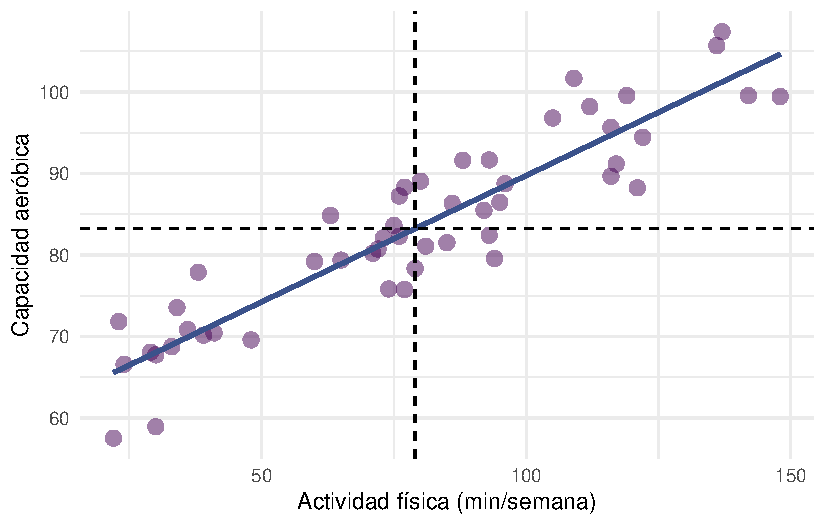
\includegraphics[width=0.85\linewidth,height=\textheight,keepaspectratio]{unidad_3/03_covarianza_correlacion_files/figure-pdf/cov-1-1.pdf}
\end{center}

\subsubsection{Covarianza negativa}\label{covarianza-negativa}

En este gráfico, a medida que aumenta el consumo de alcohol semanal
(\(X\) ), disminuyen los niveles de enzimas hepáticas (\(Y\)). Casi
todos los puntos pertenecen a los cuadrantes segundo y cuarto
(\(S_{XY}<0\)).

\begin{center}
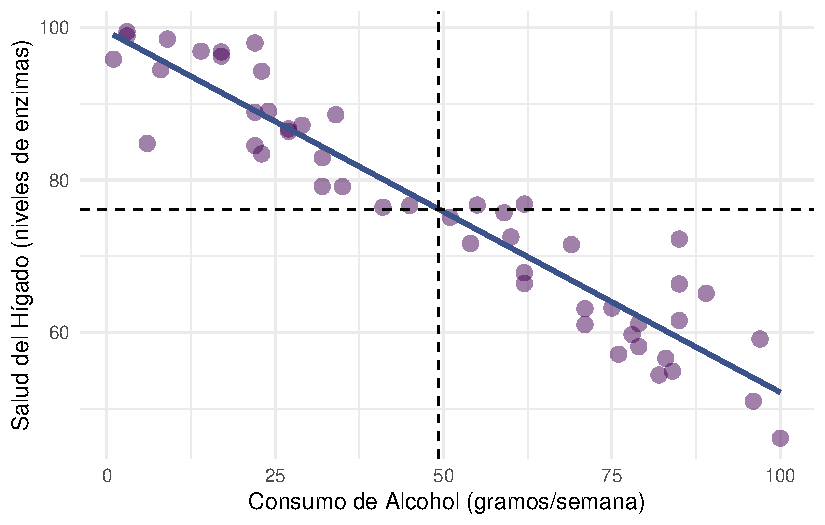
\includegraphics[width=0.85\linewidth,height=\textheight,keepaspectratio]{unidad_3/03_covarianza_correlacion_files/figure-pdf/cov-2-1.pdf}
\end{center}

\subsubsection{Covarianza cercana a
cero}\label{covarianza-cercana-a-cero}

En el diagrama de dispersión se puede observar que los cambios en las
horas de sueño (\(X\)) no tienen relación con el nivel de colesterol en
sangre (\(Y\)). No se observa un patrón, sino que los puntos se reparten
de modo más o menos homogéneo entre los cuadrantes (\(S_{XY}\simeq 0\)).

\begin{center}
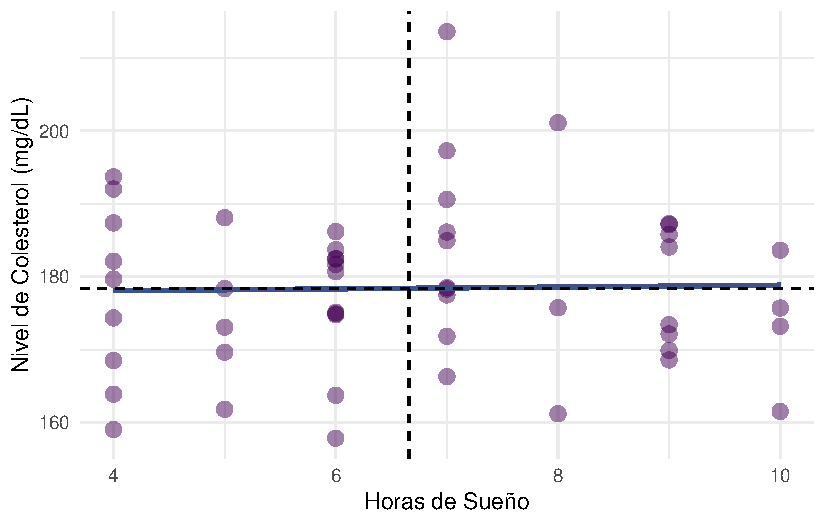
\includegraphics[width=0.85\linewidth,height=\textheight,keepaspectratio]{unidad_3/03_covarianza_correlacion_files/figure-pdf/cov-3-1.pdf}
\end{center}

\subsection{Limitaciones de la
covarianza}\label{limitaciones-de-la-covarianza}

La covarianza está afectada por las unidades en las que se miden las
variables, lo que puede dificultar la interpretación de su magnitud.
Para resolver este problema, es necesario utilizar una medida que no
esté afectada por las unidades de medida de las variables: la
\textbf{correlación.}

\section{Correlación}\label{correlaciuxf3n}

La correlación trata de establecer la relación o dependencia que existe
entre las dos variables que intervienen en una distribución
bidimensional. Es decir, determinar si los cambios en una de las
variables influyen en los cambios de la otra. En caso de que suceda,
diremos que las variables están correlacionadas o que hay correlación
entre ellas.

La correlación, como cuantificación del grado de relación que hay entre
dos variables, es un valor entre -1 y +1, pasando, por el cero. Hay, por
lo tanto, correlaciones positivas y negativas. El \textbf{signo} es,
pues, el primer elemento básico a tener en cuenta.

\begin{itemize}
\item
  \textbf{Correlación positiva}: existe relación directa; ambas
  variables aumentan o disminuyen simultáneamente. El coeficiente de
  correlación tiene valores entre 0 y 1.
\item
  \textbf{Correlación negativa}: existe relación inversa; una variable
  aumenta mientras la otra disminuye. El coeficiente de correlación
  tiene valores entre -1 y 0.
\item
  \textbf{Correlación cercana a cero}: no hay relación lineal, aunque
  podría existir una relación no lineal.
\end{itemize}

Lo segundo a tener en cuenta en la correlación es la \textbf{magnitud}.
Y esto lo marca el valor absoluto de la correlación. En la magnitud se
valora la correlación sin el signo, valorando la magnitud del número
puro. Esto significa que cuanto más cerca estemos de los extremos del
intervalo de valores posibles: -1 y +1, más correlación tenemos.

La correlación más usada para variables cuantitativas es la
\textbf{correlación de Pearson}. Es especialmente apropiada cuando la
distribución de las variables es la normal. Si no se cumple la
normalidad o si las variables son ordinales es más apropiado usar la
\textbf{correlación de Spearman} o la \textbf{correlación de Kendall}.

\subsection{Correlación de Pearson}\label{correlaciuxf3n-de-pearson}

Mide la relación lineal entre dos variables, eliminando la influencia de
las unidades de medida. Es una medida adimensional, obtenida al
estandarizar la covarianza entre dos variables \(X\) e \(Y\):

\[
r = \frac{Cov_{XY}}{S_xS_y} 
\]

donde:

\begin{itemize}
\item
  \(Cov_{XY}\) es la covarianza entre las variables \(X\) e \(Y\).
\item
  \(S_x\) y \(S_y\) son las desviaciones estándar de las variables \(X\)
  e \(Y\).
\end{itemize}

El coeficiente de correlación \(r\) entonces se interpreta como:

\begin{itemize}
\item
  \(0 < r \leq 1\): correlación positiva; ambas variables aumentan o
  disminuyen simultáneamente.
\item
  \(-1 \leq r > 0\): correlación negativa; una variable aumenta mientras
  la otra disminuye.
\item
  \(r ≈ 0\): no hay relación lineal, aunque podría existir una relación
  no lineal.
\end{itemize}

¿A partir de qué valores de \(r\) se considera que hay \emph{``buena
correlación''}? La respuesta no es simple. Hay que tener en cuenta la
presencia de observaciones anómalas y si la varianza se mantiene
homogénea. En reglas generales se acepta que:

\begin{itemize}
\item
  \(r ≈ ±1\): correlación perfecta.
\item
  \(r \geq ±0.7\): correlación fuerte.
\item
  \(±0.4 \leq r < ±0.7\): correlación moderada.
\item
  \(r \leq ±0.4\): correlación débil.
\end{itemize}

\subsubsection{\texorpdfstring{Correlación positiva perfecta entre \(X\)
e
\(Y\)}{Correlación positiva perfecta entre X e Y}}\label{correlaciuxf3n-positiva-perfecta-entre-x-e-y}

\begin{center}
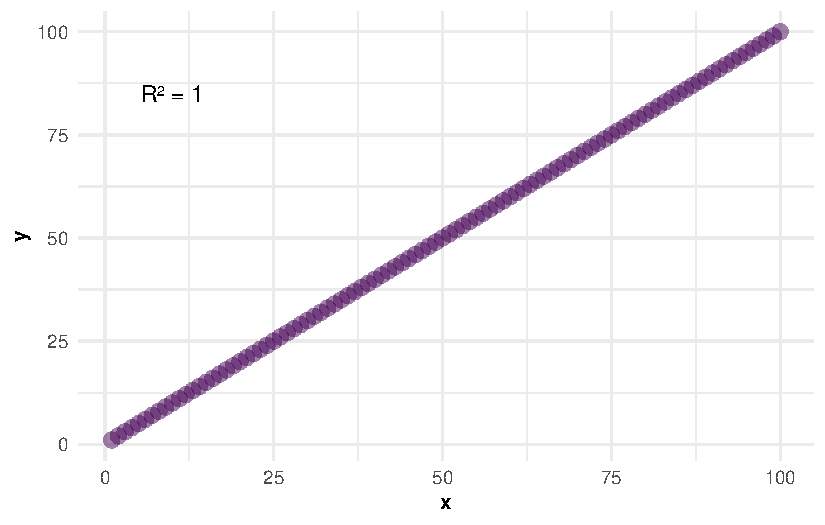
\includegraphics[width=0.85\linewidth,height=\textheight,keepaspectratio]{unidad_3/03_covarianza_correlacion_files/figure-pdf/cor-1-1.pdf}
\end{center}

\subsubsection{\texorpdfstring{Correlación positiva fuerte entre \(X\) e
\(Y\)}{Correlación positiva fuerte entre X e Y}}\label{correlaciuxf3n-positiva-fuerte-entre-x-e-y}

\begin{center}
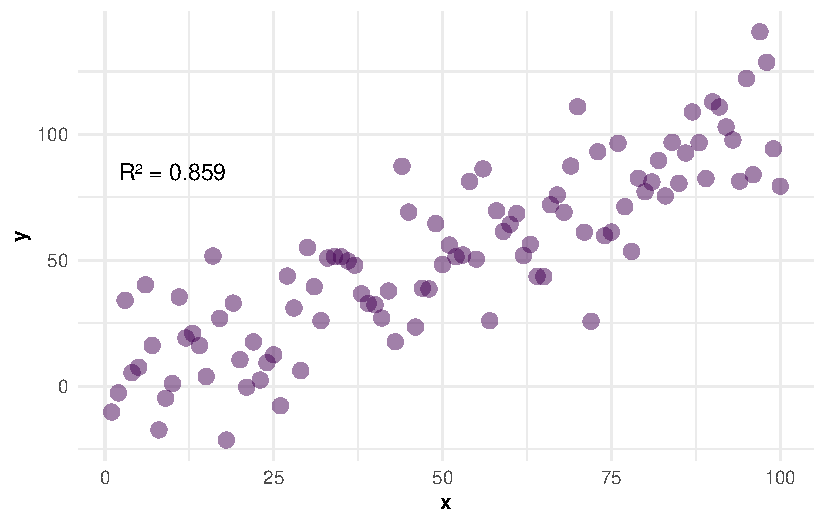
\includegraphics[width=0.85\linewidth,height=\textheight,keepaspectratio]{unidad_3/03_covarianza_correlacion_files/figure-pdf/cor-2-1.pdf}
\end{center}

\subsubsection{\texorpdfstring{Correlación positiva moderada entre \(X\)
e
\(Y\)}{Correlación positiva moderada entre X e Y}}\label{correlaciuxf3n-positiva-moderada-entre-x-e-y}

\begin{center}
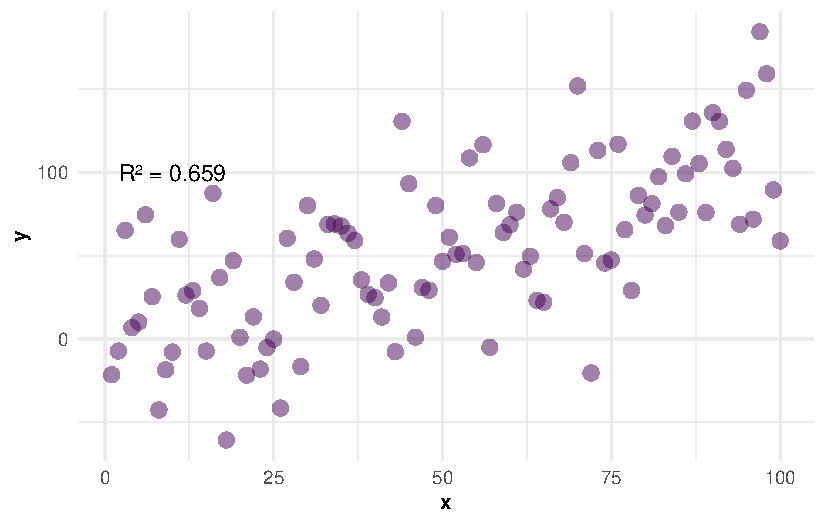
\includegraphics[width=0.85\linewidth,height=\textheight,keepaspectratio]{unidad_3/03_covarianza_correlacion_files/figure-pdf/cor-3-1.pdf}
\end{center}

\subsubsection{\texorpdfstring{Correlación negativa perfecta entre \(X\)
e
\(Y\)}{Correlación negativa perfecta entre X e Y}}\label{correlaciuxf3n-negativa-perfecta-entre-x-e-y}

\begin{center}
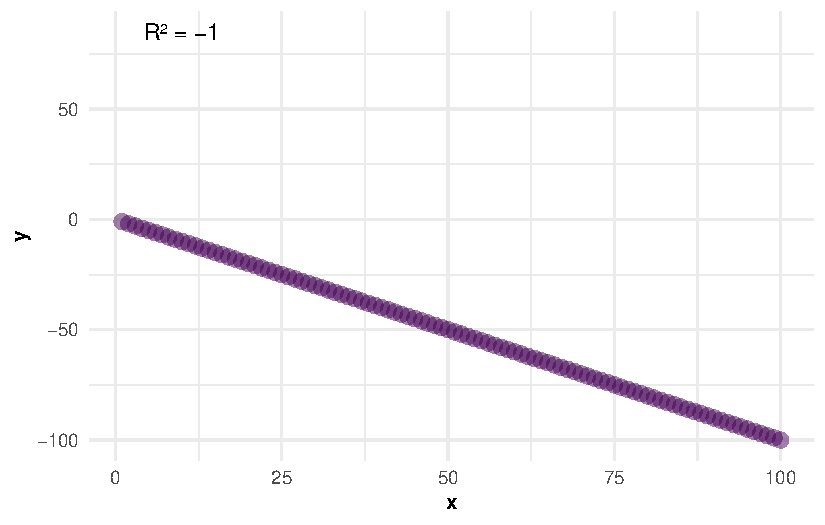
\includegraphics[width=0.85\linewidth,height=\textheight,keepaspectratio]{unidad_3/03_covarianza_correlacion_files/figure-pdf/cor-4-1.pdf}
\end{center}

\subsubsection{\texorpdfstring{Correlación negativa fuerte entre \(X\) e
\(Y\)}{Correlación negativa fuerte entre X e Y}}\label{correlaciuxf3n-negativa-fuerte-entre-x-e-y}

\begin{center}
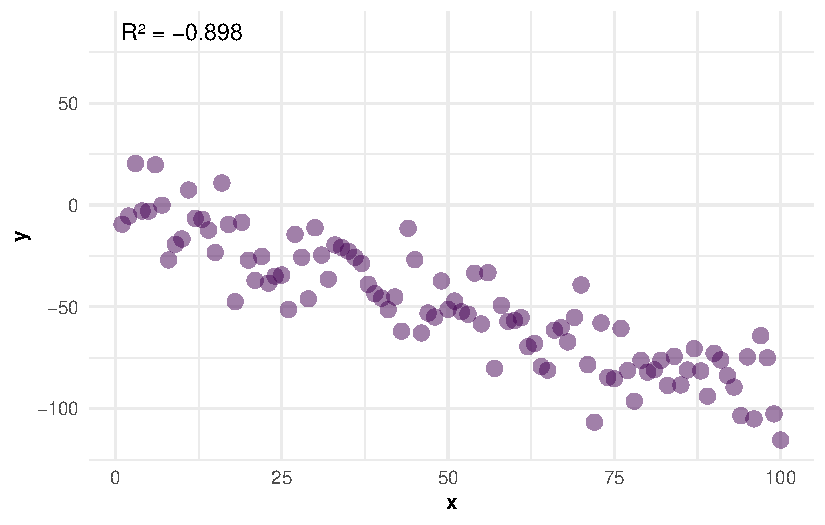
\includegraphics[width=0.85\linewidth,height=\textheight,keepaspectratio]{unidad_3/03_covarianza_correlacion_files/figure-pdf/cor-5-1.pdf}
\end{center}

\subsubsection{\texorpdfstring{Correlación negativa moderada entre \(X\)
e
\(Y\)}{Correlación negativa moderada entre X e Y}}\label{correlaciuxf3n-negativa-moderada-entre-x-e-y}

\begin{center}
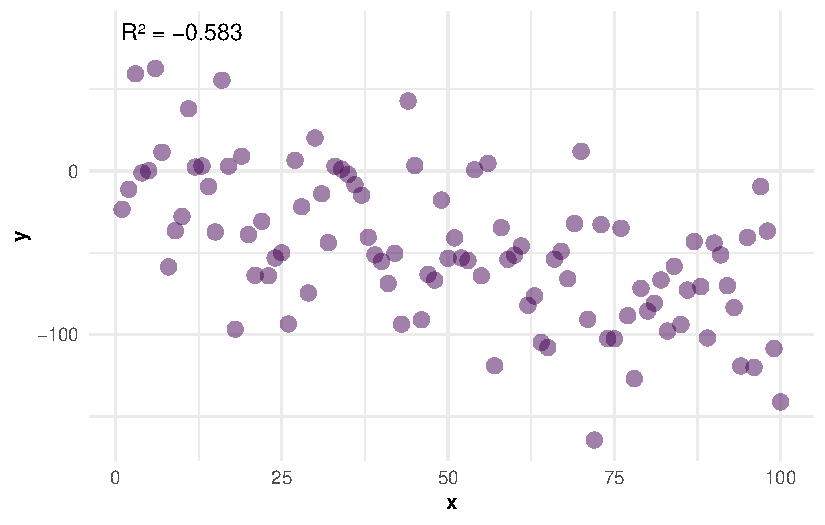
\includegraphics[width=0.85\linewidth,height=\textheight,keepaspectratio]{unidad_3/03_covarianza_correlacion_files/figure-pdf/cor-6-1.pdf}
\end{center}

\subsubsection{\texorpdfstring{\(X\) e \(Y\) no
correlacionadas}{X e Y no correlacionadas}}\label{x-e-y-no-correlacionadas}

\begin{center}
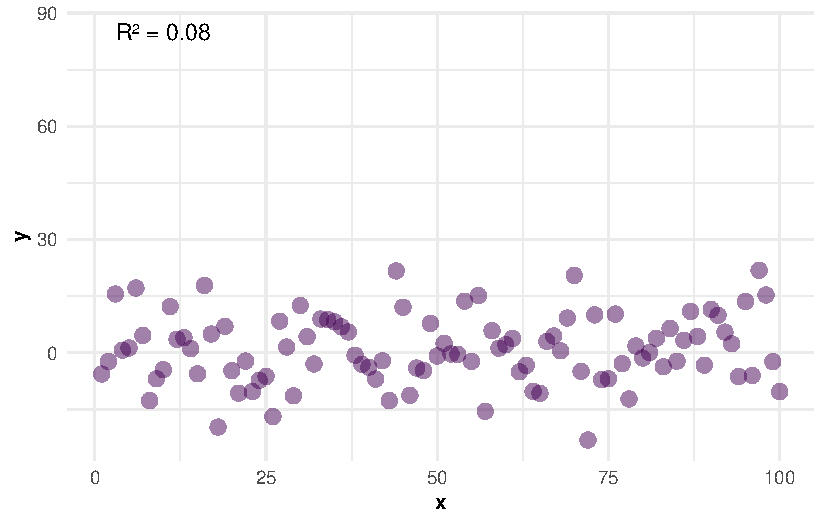
\includegraphics[width=0.85\linewidth,height=\textheight,keepaspectratio]{unidad_3/03_covarianza_correlacion_files/figure-pdf/cor-7-1.pdf}
\end{center}

\subsubsection{\texorpdfstring{Relación no lineal entre \(X\) e
\(Y\)}{Relación no lineal entre X e Y}}\label{relaciuxf3n-no-lineal-entre-x-e-y}

\begin{center}
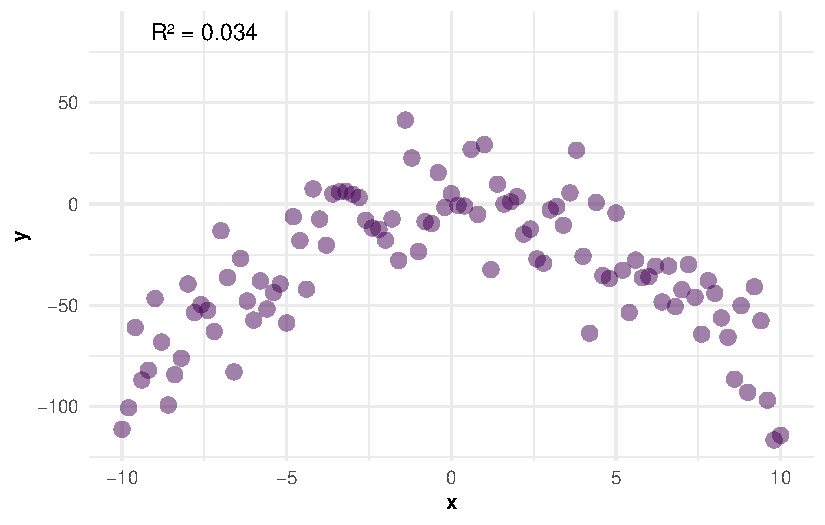
\includegraphics[width=0.85\linewidth,height=\textheight,keepaspectratio]{unidad_3/03_covarianza_correlacion_files/figure-pdf/cor-8-1.pdf}
\end{center}

\subsubsection{Correlogramas}\label{correlogramas}

Los correlogramas son gráficos que muestra la relación entre cada par de
variables numéricas en un conjunto de datos. Se utiliza para analizar la
correlación entre variables, identificar patrones y controlar la
aleatoriedad de los datos. Existen diversos paquetes en R que permiten
generar correlogramas, como \texttt{correlation}, que forma parte del
ecosistema de paquetes \texttt{easystats} (Lüdecke et~al. 2022), o
\texttt{GGally}(Schloerke et~al. 2025) que usa como base el paquete
\texttt{ggplot2}.

\subsection{Correlación de Spearman}\label{correlaciuxf3n-de-spearman}

Mide la correlación entre dos variables basada en los \textbf{rangos}
(orden) de los valores. Se utiliza cuando los datos \textbf{no presentan
una relación lineal} o tienen una relación monótona. Matemáticamente se
expresa como:

\[
\rho = \frac{1 - 6\sum d_i^2}{n(n^2-1)}
\]

donde:

\begin{itemize}
\item
  \(d_i\) es la diferencia en los rangos de cada par de observaciones.
\item
  \(n\) es el número de observaciones.
\end{itemize}

\subsection{Correlación de Kendall}\label{correlaciuxf3n-de-kendall}

Mide la relación ordinal entre dos variables numéricas en base a la
\textbf{concordancia} y \textbf{discordancia} entre pares. Se utiliza
cuando hay datos con valores repetidos o la muestra es pequeña. Es más
robusta frente a datos con valores atípicos en comparación con Spearman.
Matemáticamente se expresa como:

\[
\tau = \frac{n_c - n_d}{n(n-1)/2}
\]

donde:

\begin{itemize}
\tightlist
\item
  \(n_c\) y \(n_d\) son los pares concordantes o discordantes.
\end{itemize}

\section{Ejemplo práctico en R}\label{ejemplo-pruxe1ctico-en-r-4}

Tomemos como ejemplo la base \texttt{cancer\_USA.txt} que contiene
información sobre la tasa de mortalidad por cáncer cada 100.000
habitantes de distintos condados de la Costa Este de Estados Unidos.

Comenzaremos por cargar los paquetes necesarios para el análisis:

\begin{Shaded}
\begin{Highlighting}[]
\CommentTok{\# Gráficos de correlación}
\FunctionTok{library}\NormalTok{(easystats)}

\FunctionTok{library}\NormalTok{(GGally)}

\CommentTok{\# Manejo de datos}
\FunctionTok{library}\NormalTok{(tidyverse)}
\end{Highlighting}
\end{Shaded}

Cargamos los datos y exploramos su estructura:

\begin{Shaded}
\begin{Highlighting}[]
\CommentTok{\# Carga de datos}
\NormalTok{datos }\OtherTok{\textless{}{-}} \FunctionTok{read\_csv2}\NormalTok{(}\StringTok{"datos/cancer\_USA.txt"}\NormalTok{)}

\CommentTok{\# Explora datos}
\FunctionTok{glimpse}\NormalTok{(datos)}
\end{Highlighting}
\end{Shaded}

\begin{verbatim}
Rows: 213
Columns: 10
$ condado            <chr> "Belknap County", "Carroll County", "Cheshire Count~
$ estado             <chr> "New Hampshire", "New Hampshire", "New Hampshire", ~
$ tasa_mortalidad    <dbl> 182.6, 168.8, 162.8, 181.6, 155.0, 163.2, 173.1, 17~
$ mediana_edad       <dbl> 46.1, 50.3, 42.0, 48.1, 41.9, 40.1, 42.6, 43.5, 37.~
$ mediana_edad_cat   <chr> "45+ años", "45+ años", "36-39 años", "45+ años", "~
$ mediana_ingresos   <dbl> 59831, 57556, 56008, 42491, 56353, 71233, 62429, 79~
$ pct_pobreza        <dbl> 10.0, 10.7, 11.8, 14.9, 11.6, 8.7, 9.5, 6.1, 11.8, ~
$ pct_salud_publica  <dbl> 16.8, 13.4, 12.7, 22.5, 14.0, 12.7, 13.1, 9.0, 12.4~
$ pct_sec_incompleta <dbl> 15.4, 14.8, 6.1, 13.2, 6.6, 12.9, 10.9, 13.5, 6.1, ~
$ pct_desempleo      <dbl> 5.3, 5.8, 6.1, 6.9, 5.0, 5.9, 5.2, 5.6, 6.5, 5.8, 1~
\end{verbatim}

La base de datos tiene 213 observaciones y 10 variables. La variable
dependiente es \texttt{tasa\_mortalidad} y hay 3 variables
independientes categóricas y 6 variables independientes numéricas o
continuas:

\begin{itemize}
\item
  \texttt{tasa\_mortalidad}: Tasa de mortalidad por cáncer a nivel de
  condado (datos agregados).
\item
  \texttt{pct\_salud\_publica}: Porcentaje de personas con cobertura
  exclusiva de salud pública en el condado.
\item
  \texttt{pct\_pobreza}: Porcentaje de personas por debajo de la línea
  de pobreza en el condado.
\item
  \texttt{pct\_sec\_incompleta}: Porcentaje de personas con estudios
  secundarios incompletos en el condado.
\item
  \texttt{mediana\_edad}: Mediana de la edad de fallecimiento por cáncer
  en el condado.
\item
  \texttt{mediana\_edad\_cat}: Versión categorizada de la mediana de
  edad al fallecer por cáncer en el condado.
\item
  \texttt{condado}: Condado de residencia.
\item
  \texttt{estado}: Estado de residencia.
\end{itemize}

La función \texttt{cor()} estima la correlación entre dos variables. El
método predeterminado devuelve la correlación de Pearson y puede
modificarse el argumento \texttt{method} para obtener la correlación de
Kendall o Spearman:

\begin{Shaded}
\begin{Highlighting}[]
\FunctionTok{cor}\NormalTok{(datos}\SpecialCharTok{$}\NormalTok{tasa\_mortalidad, datos}\SpecialCharTok{$}\NormalTok{pct\_pobreza, }\AttributeTok{method =} \StringTok{"pearson"}\NormalTok{)}
\end{Highlighting}
\end{Shaded}

\begin{verbatim}
[1] 0.3301532
\end{verbatim}

La función \texttt{cor.test()} determina si la prueba de correlación de
Pearson calculada es significativa mediante el estadístico \(t\) de
Student:

\begin{Shaded}
\begin{Highlighting}[]
\FunctionTok{cor.test}\NormalTok{(datos}\SpecialCharTok{$}\NormalTok{tasa\_mortalidad, datos}\SpecialCharTok{$}\NormalTok{pct\_pobreza)}
\end{Highlighting}
\end{Shaded}

\begin{verbatim}

    Pearson's product-moment correlation

data:  datos$tasa_mortalidad and datos$pct_pobreza
t = 5.0806, df = 211, p-value = 8.266e-07
alternative hypothesis: true correlation is not equal to 0
95 percent confidence interval:
 0.2048117 0.4448414
sample estimates:
      cor 
0.3301532 
\end{verbatim}

Los resultados de la función son:

\begin{itemize}
\tightlist
\item
  El valor del estadístico \(t\)
\item
  El valor de \(p\) para el estadístico
\item
  El valor de la correlación de Pearson
\item
  Los intervalos de confianza para la correlación
\end{itemize}

Los argumentos predeterminados para la función \texttt{cor.test()} son:

\begin{itemize}
\item
  \texttt{alternative\ =\ "two.sided"} - indica la hipotesis
  alternativa, también puede ser \texttt{"greater"} para asociación
  positiva, \texttt{"less"} para asociación negativa.
\item
  \texttt{conf.level\ =\ 0.95} - determina el nivel de confianza (se
  puede modificar).
\item
  \texttt{method\ =\ "pearson"} - especifíca el tipo de test de
  correlación. También permite \texttt{"kendall"} o \texttt{"spearman".}
\end{itemize}

\subsection{Gráficos de
correlación}\label{gruxe1ficos-de-correlaciuxf3n}

Podemos generar diagramas de dispersión para cada par de variables
numéricas usando la función \texttt{ggpairs()} del paquete
\texttt{GGally} (Schloerke et~al. 2025):

\begin{Shaded}
\begin{Highlighting}[]
\NormalTok{datos }\SpecialCharTok{|\textgreater{}}
  \CommentTok{\# selecciono soloamente las variables numéricas}
  \FunctionTok{select}\NormalTok{(}\FunctionTok{where}\NormalTok{(is.numeric)) }\SpecialCharTok{|\textgreater{}}

  \CommentTok{\# diagramas de dispersión}
  \FunctionTok{ggpairs}\NormalTok{()}
\end{Highlighting}
\end{Shaded}

\begin{center}
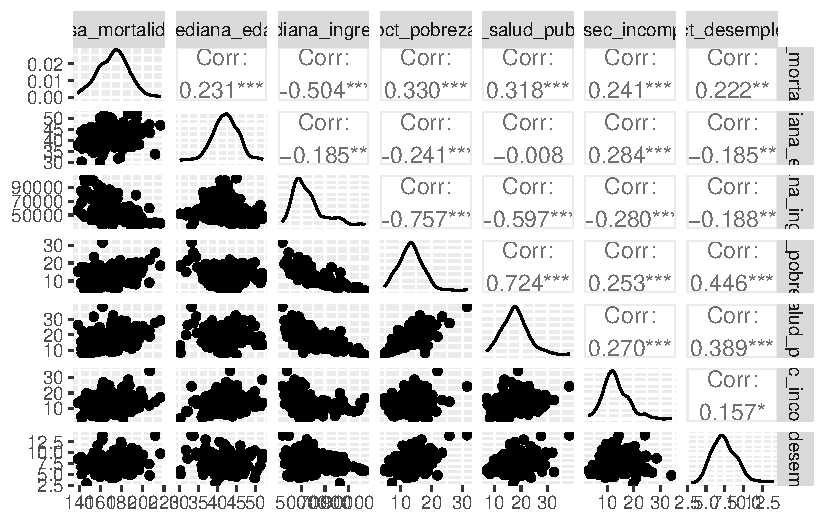
\includegraphics[width=0.85\linewidth,height=\textheight,keepaspectratio]{unidad_3/03_covarianza_correlacion_files/figure-pdf/ej5-1.pdf}
\end{center}

Podemos generar los correlogramas con el paquete \texttt{correlation}
usando el siguiente código:

\begin{Shaded}
\begin{Highlighting}[]
\NormalTok{datos }\SpecialCharTok{|\textgreater{}}
  \FunctionTok{correlation}\NormalTok{() }\SpecialCharTok{|\textgreater{}}
  \FunctionTok{summary}\NormalTok{() }\SpecialCharTok{|\textgreater{}}
  \FunctionTok{plot}\NormalTok{()}
\end{Highlighting}
\end{Shaded}

\begin{center}
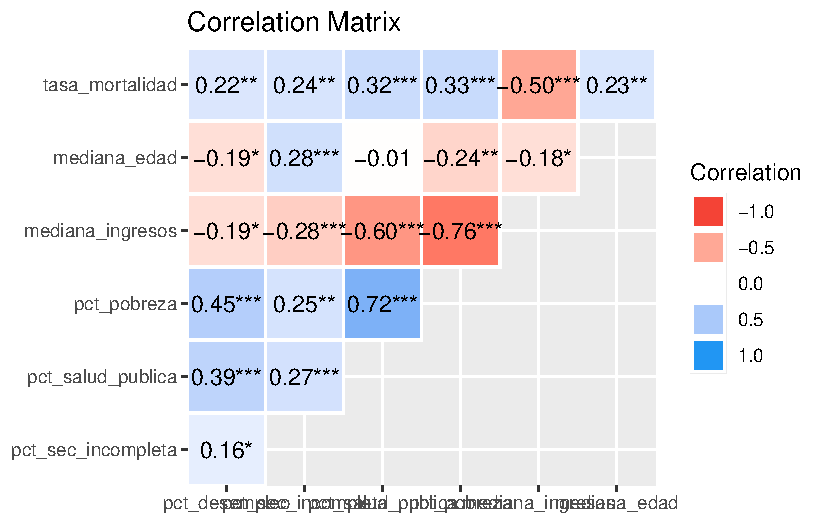
\includegraphics[width=0.85\linewidth,height=\textheight,keepaspectratio]{unidad_3/03_covarianza_correlacion_files/figure-pdf/ej6-1.pdf}
\end{center}

El comando \texttt{ggcorr()} del paquete \texttt{GGally} también nos
permite generar correlogramas:

\begin{Shaded}
\begin{Highlighting}[]
\NormalTok{datos }\SpecialCharTok{|\textgreater{}}
  \CommentTok{\# selecciono soloamente las variables numéricas}
  \FunctionTok{select}\NormalTok{(}\FunctionTok{where}\NormalTok{(is.numeric)) }\SpecialCharTok{|\textgreater{}}

  \CommentTok{\# correlograma}
  \FunctionTok{ggcorr}\NormalTok{(}\AttributeTok{label =}\NormalTok{ T)}
\end{Highlighting}
\end{Shaded}

\begin{center}
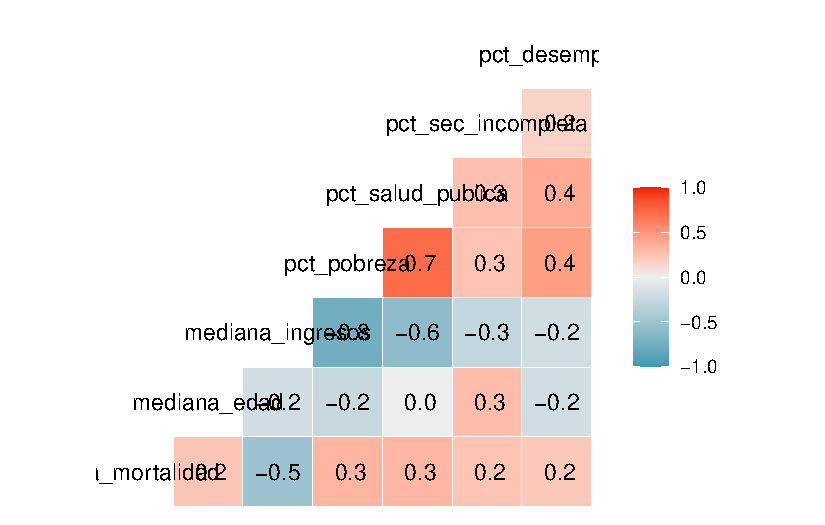
\includegraphics[width=0.85\linewidth,height=\textheight,keepaspectratio]{unidad_3/03_covarianza_correlacion_files/figure-pdf/ej7-1.pdf}
\end{center}

Podemos hacerlos más atractivos visualmente modificando los argumentos
\texttt{nbreaks}, \texttt{geom}, \texttt{size}, \texttt{max\_size} y
\texttt{palette}:

\begin{Shaded}
\begin{Highlighting}[]
\NormalTok{datos }\SpecialCharTok{|\textgreater{}}
  \CommentTok{\# selecciono soloamente las variables numéricas}
  \FunctionTok{select}\NormalTok{(}\FunctionTok{where}\NormalTok{(is.numeric)) }\SpecialCharTok{|\textgreater{}}

  \CommentTok{\# correlograma}
  \FunctionTok{ggcorr}\NormalTok{(}
    \AttributeTok{label =}\NormalTok{ T, }\CommentTok{\# coeficientes}
    \AttributeTok{size =} \DecValTok{3}\NormalTok{, }\CommentTok{\# tamaño de texto}
    \AttributeTok{geom =} \StringTok{"circle"}\NormalTok{, }\CommentTok{\# forma del gráfico}
    \AttributeTok{max\_size =} \DecValTok{15}\NormalTok{, }\CommentTok{\# tamaño máximo de las formas}
    \AttributeTok{nbreaks =} \DecValTok{6}\NormalTok{, }\CommentTok{\# número de categorías de color}
    \AttributeTok{palette =} \StringTok{"PRGn"}
\NormalTok{  ) }\CommentTok{\# color de las formas}
\end{Highlighting}
\end{Shaded}

\begin{center}
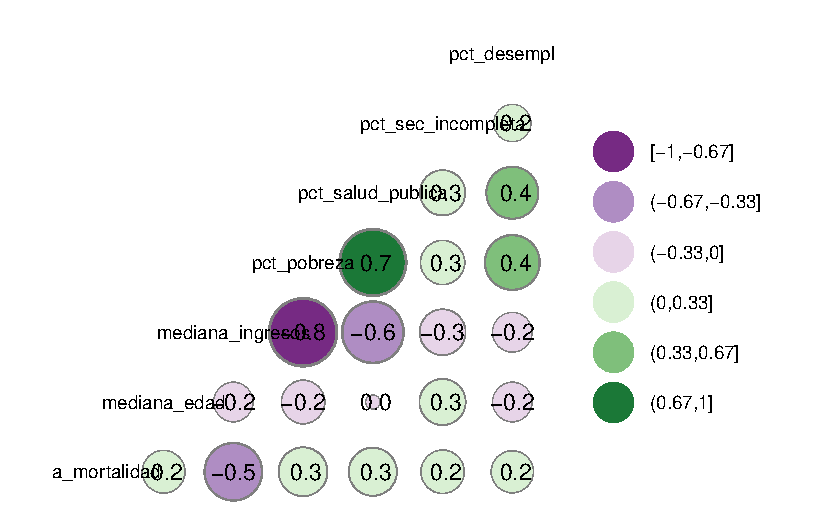
\includegraphics[width=0.85\linewidth,height=\textheight,keepaspectratio]{unidad_3/03_covarianza_correlacion_files/figure-pdf/ej8-1.pdf}
\end{center}

Observamos que la variable dependiente (\texttt{tasa\_mortalidad}) tiene
correlación negativa moderada con \texttt{mediana\_ingresos}, también
que existe una correlación negativa fuerte entre \texttt{pct\_pobreza} y
\texttt{mediana\_ingresos} y moderada con \texttt{pct\_salud\_publica}.
Las correlaciones entre las demás variables son débiles o nulas.

Para visualizar el correlograma con el coeficiente de Spearman, añadimos
el argumento \texttt{method\ =\ c("pairwise",\ "spearman")} al código
del ejemplo anterior:

\begin{Shaded}
\begin{Highlighting}[]
\NormalTok{datos }\SpecialCharTok{|\textgreater{}}
  \CommentTok{\# selecciono soloamente las variables numéricas}
  \FunctionTok{select}\NormalTok{(}\FunctionTok{where}\NormalTok{(is.numeric)) }\SpecialCharTok{|\textgreater{}}

  \CommentTok{\# correlograma}
  \FunctionTok{ggcorr}\NormalTok{(}
    \AttributeTok{label =}\NormalTok{ T, }\CommentTok{\# coeficientes}
    \AttributeTok{size =} \DecValTok{3}\NormalTok{, }\CommentTok{\# tamaño de texto}
    \AttributeTok{geom =} \StringTok{"circle"}\NormalTok{, }\CommentTok{\# forma del gráfico}
    \AttributeTok{max\_size =} \DecValTok{15}\NormalTok{, }\CommentTok{\# tamaño máximo de las formas}
    \AttributeTok{nbreaks =} \DecValTok{6}\NormalTok{, }\CommentTok{\# número de categorías de color}
    \AttributeTok{palette =} \StringTok{"PRGn"}\NormalTok{, }\CommentTok{\# color de las formas}
    \AttributeTok{method =} \FunctionTok{c}\NormalTok{(}\StringTok{"pairwise"}\NormalTok{, }\StringTok{"spearman"}\NormalTok{)}
\NormalTok{  ) }\CommentTok{\# coeficiente de Spearman}
\end{Highlighting}
\end{Shaded}

\begin{center}
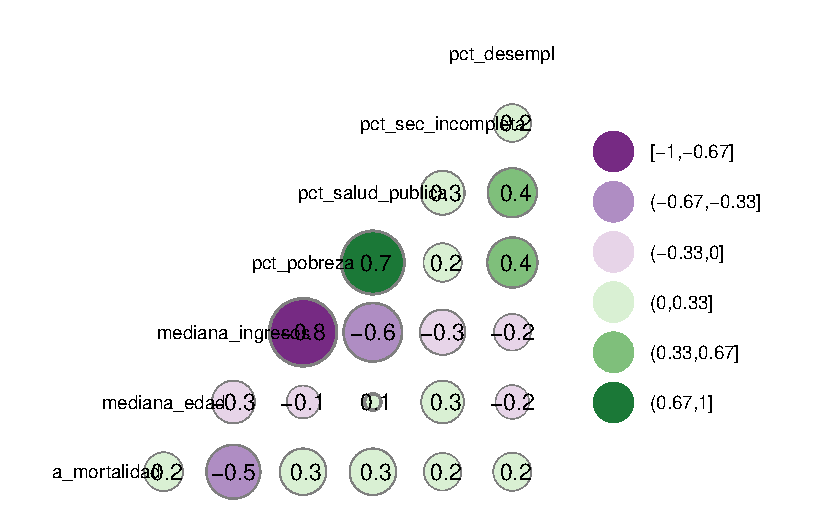
\includegraphics[width=0.85\linewidth,height=\textheight,keepaspectratio]{unidad_3/03_covarianza_correlacion_files/figure-pdf/ej9-1.pdf}
\end{center}

De igual modo, si queremos aplicar el coeficiente de Spearman, añadimos
el argumento \texttt{method\ =\ c("pairwise",\ "kendall")}:

\begin{Shaded}
\begin{Highlighting}[]
\NormalTok{datos }\SpecialCharTok{|\textgreater{}}
  \CommentTok{\# selecciono soloamente las variables numéricas}
  \FunctionTok{select}\NormalTok{(}\FunctionTok{where}\NormalTok{(is.numeric)) }\SpecialCharTok{|\textgreater{}}

  \CommentTok{\# correlograma}
  \FunctionTok{ggcorr}\NormalTok{(}
    \AttributeTok{label =}\NormalTok{ T, }\CommentTok{\# coeficientes}
    \AttributeTok{size =} \DecValTok{3}\NormalTok{, }\CommentTok{\# tamaño de texto}
    \AttributeTok{geom =} \StringTok{"circle"}\NormalTok{, }\CommentTok{\# forma del gráfico}
    \AttributeTok{max\_size =} \DecValTok{15}\NormalTok{, }\CommentTok{\# tamaño máximo de las formas}
    \AttributeTok{nbreaks =} \DecValTok{6}\NormalTok{, }\CommentTok{\# número de categorías de color}
    \AttributeTok{palette =} \StringTok{"PRGn"}\NormalTok{, }\CommentTok{\# color de las formas}
    \AttributeTok{method =} \FunctionTok{c}\NormalTok{(}\StringTok{"pairwise"}\NormalTok{, }\StringTok{"kendall"}\NormalTok{)}
\NormalTok{  ) }\CommentTok{\# coeficiente de Kendall}
\end{Highlighting}
\end{Shaded}

\begin{center}
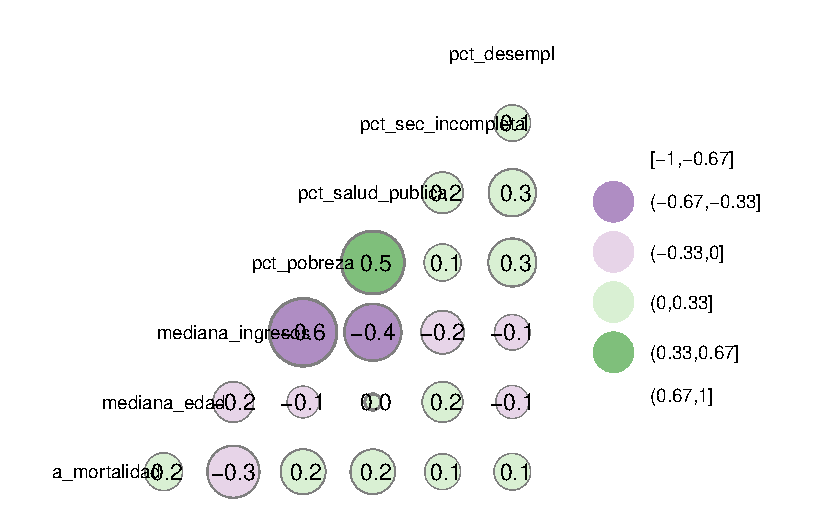
\includegraphics[width=0.85\linewidth,height=\textheight,keepaspectratio]{unidad_3/03_covarianza_correlacion_files/figure-pdf/ej10-1.pdf}
\end{center}

Para explicar la forma de esta correlación e incluso predecir los
valores que puede alcanzar una variable dependiente numérica en función
de una variable independiente también numérica podemos utilizar la
\href{04_reg_lineal.qmd}{\textbf{regresión lineal simple}}.

Triola (2018)

Agresti (2015)

Wickham et~al. (2019)

\section*{Referencias}\label{referencias-13}
\addcontentsline{toc}{section}{Referencias}

\markright{Referencias}

\chapter{Regresión lineal simple}\label{regresiuxf3n-lineal-simple}

\section{Introducción}\label{introducciuxf3n-13}

Para entender el modelo de regresión lineal simple, volvamos al ejemplo
del peso en niñas menores de 6 meses de la
\hyperref[ejemplo-pruxe1ctico-en-r]{\textbf{unidad anterior}}, donde
habíamos trazado una recta que nos ilustraba la relación lineal del peso
en función de la edad.

Según el modelo estadístico para la función lineal de \(Y\) según \(X\):

\[
Y(X) =  \beta_0 + \beta_1 + X_1
\]

Hemos ajustado un modelo cuyos parámetros son:

\[
\hat{y} = b_0 + b_1X_1
\]

donde \(b_1\) nos está indicando cuánto se modifica \(\hat{y}\) por cada
unidad de aumento de \(X_1\).

\[
\hat{y} = 2468,9 + 100,7 \: edad \: (en \: semanas) 
\]

Se interpreta que por cada semana este grupo de lactantes ha aumentado
en promedio 100 gramos, o que cada 1 mes (4 semanas) aumentan una media
de 400 gramos.

Podemos observar que hay una relación lineal y que esta relación no es
perfecta. Existe cierta dispersión entre los puntos sugiriendo que
alguna variación en el peso no se asocia con un incremento de la edad
(por ejemplo dos lactantes de 15 semanas. Tienen la misma edad y 1.600
grs de diferencia. Cabría preguntarse si esas niñas que se ``alejan''
tanto de la recta de regresión no tienen algún antecedente distinto del
resto). Más adelante veremos cómo se interpretan esas diferentes
distancias entre las observaciones y la recta de regresión.

Ahora vamos a concentrarnos en la relación entre la varianza de la
muestra, a través del desvío estándar (\(ds = \sqrt{varianza}\)) y la
magnitud de la asociación. Se muestran cuatro ejemplos en los cuáles se
fue aumentando progresivamente el desvío estándar de los datos. Observen
cómo a medida que aumenta la variabilidad entre los individuos va
disminuyendo el coeficiente de correlación y el coeficiente \(b_1\)
(pendiente de la recta)

\begin{center}
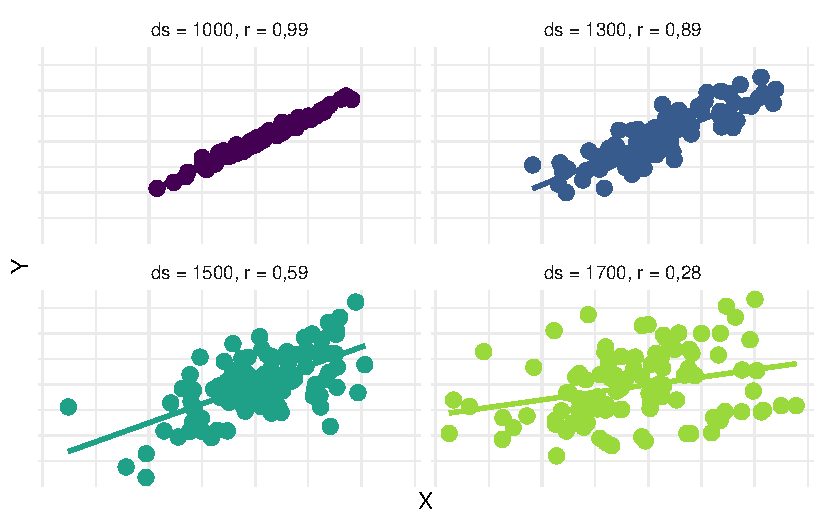
\includegraphics[width=0.85\linewidth,height=\textheight,keepaspectratio]{unidad_3/04_reg_lineal_files/figure-pdf/fig1-1.pdf}
\end{center}

Podemos observar que cuanto mayor es la varianza en una muestra:

\begin{itemize}
\item
  Mayor es la variabilidad de \(y\) en torno a la recta de regresión
\item
  Mayor es la imprecisión asociada a la estimativa de los parámetros de
  regresión
\end{itemize}

\section{Presupuestos del modelo}\label{presupuestos-del-modelo}

Cuando planeamos realizar un análisis de regresión con un conjunto de
datos es necesario saber que para que podamos plantearlo adecuadamente
deben cumplirse ciertas condiciones, que llamaremos Presupuestos del
modelo:

\begin{enumerate}
\def\labelenumi{\arabic{enumi}.}
\tightlist
\item
  Independencia: los valores de \(y\) deben ser independientes unos de
  otros
\item
  Linealidad: la relación entre \(x\) e \(y\) debe ser una función
  lineal
\item
  Homocedasticidad: la varianza de \(y\) debe mantenerse constante para
  los distintos valores de \(x\)
\item
  Normalidad: \(y\) debe tener una distribución normal
\end{enumerate}

\textbf{¿Cómo se obtiene la recta de regresión? ¿Cómo se calculan los
coeficientes de la regresión?}

En el ejemplo del peso según edad en niñas menores de 6 meses, la idea
es encontrar una función lineal (que gráficamente es una recta) que
aplicada a los valores de \(x\) nos permita aproximar los valores de
\(y\). La ecuación de la recta que describe la relación entre \(x\) e
\(y\):

\[
\hat{y} = b_0 + b_1x
\]

Por muy bueno que sea el modelo de regresión \(y\) e \(\hat{y}\) rara
vez coincidirán.

Entonces podríamos pensar que la mejor recta que permita predecir (o
aproximar) los valores de \(y\) en función de \(x\) es aquella que
minimice estos errores residuales (que algunos serán en más y otros
serán en menos).

Gráficamente:

\begin{center}
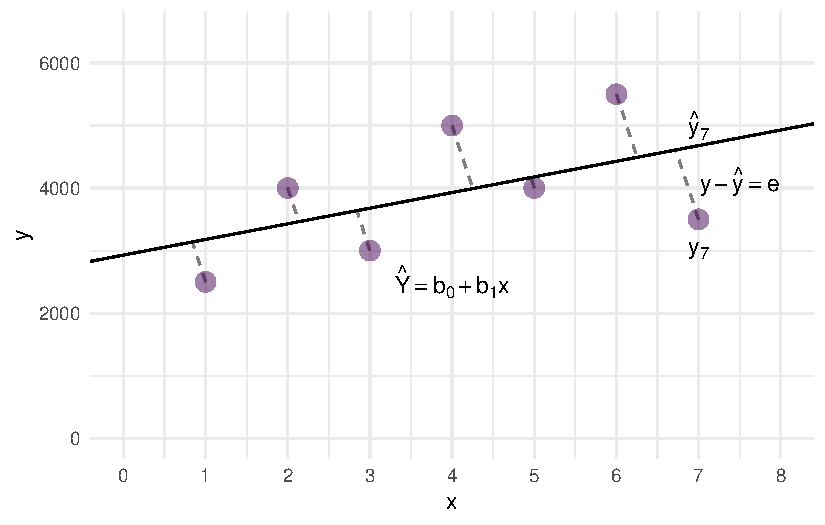
\includegraphics[width=0.85\linewidth,height=\textheight,keepaspectratio]{unidad_3/04_reg_lineal_files/figure-pdf/rls-2-1.pdf}
\end{center}

donde:

\begin{itemize}
\item
  \(\hat{y}\) es la ecuación de la ``mejor'' recta que puede trazarse
  entre estos puntos
\item
  \(b_0\) es la ordenada al origen o constante, también llamada alfa. Es
  el punto donde la recta de regresión corta al eje de ordenadas.
\item
  \(b_1\) es la pendiente de la recta (más adelante veremos cuál es la
  interpretación de estos coeficientes).
\end{itemize}

Consideremos qué pasa en el caso de la niña 7. Veamos las distancias
para este punto.

\begin{itemize}
\item
  \(y_7\) es el valor ``real'' del peso de la niña 7.
\item
  \(\hat{y}_7\) es el valor estimado de \(y\) que obtendremos a través
  de la regresión.
\item
  \(y – \hat{y} = e\) (residuo o error residual) es el desvío de \(y\)
  del valor ajustado \(\hat{y}\) en la ecuación de la regresión
  estimada.
\end{itemize}

Para poder operar con el valor de estos errores (ya que algunos tendrán
valor positivo y otros valor negativo) se los eleva al cuadrado. Esta
técnica se denomina \textbf{``método de los mínimos cuadrados''} y
consiste en adoptar como estimativas de los parámetros de la regresión
(o sea los coeficientes \(b_0\) y \(b_1\) y por ende la recta de
regresión) los valores que minimizan la suma de los cuadrados de los
residuos o error (\textbf{SCE}) para todas las observaciones de \(y\).
Lo podemos expresar así:

\[
SCE = \sum{\hat{e}^2} = \sum{(y-\hat{y})^2}
\]

Sabíamos que:

\[
\hat{y} = b_0 + b_1x
\]

Entonces si reemplazamos:

\[
SCE = \sum_{i=1}^{i=n} (y_i-\hat{y}_i)^2 =  \sum_{i=1}^{i=n}(y_i-(\hat{\beta}_0 + \hat{\beta}_1x_1))^2
\]

Es posible obtener los estimadores \(\beta_1\) y \(\beta_0\).

\[
\hat{\beta}_1 = \frac{\sum_{i=1}^{n}(x_i - \bar{x})(y_i - \bar{y})}{\sum_{i=1}^{n}(x_i-\bar{x})^2} = \frac{S_{xy}}{S_{xx}}
\]

Otra fórmula para \(\beta_1\):

\[
\hat{\beta}_1 = \frac{\sum x_iy_i-\frac{\sum x_i \sum y_i}{n}}{\sum x_i^2 - \frac{(\sum x_i)^2}{n}}
\]

\[
\hat{\beta}_0 = \bar{y} - \beta_1\bar{x}
\]

El método de los mínimos cuadrados fue creado por \emph{Johann Carl
Friedrich Gauss} (1777-1855). Tiene además la ventaja que el promedio de
los errores residuales = 0 y que para cada estimación, la varianza del
error es mínima.

\textbf{Test de hipótesis para} \(\beta_1\) e Intervalo de Confianza
95\%

Como siempre que trabajamos con una muestra, será necesario aplicar los
procesos de inferencia. Es por eso que los softwares ofrecen un test de
hipótesis para el coeficiente.

La hipótesis nula podría entenderse como que \(x\) no logra explicar la
variación de \(y\) (entonces la pendiente de la recta sería nula)

\[
H_0: \beta_1 = 0
\]

Al calcular el modelo de regresión, todos los \emph{software} estiman el
coeficiente y el error estándar del mismo (\(SE\)) y testean el
coeficiente.

\textbf{Bondad de ajuste}

Hasta ahora hemos aprendido a explicar la variación de \(y\) según la
variación de \(x\) mediante un modelo en donde las desviaciones entre el
valor observado (``real'') y el estimado (``modelo de regresión'') son
las menores posibles.

Ahora debemos saber, según los datos que tenemos, cuán bueno es el
modelo que ajustamos (qué capacidad tiene de explicar la variabilidad de
\(y\) o, si lo quiero utilizar para realizar una predicción, cuánto se
alejará mi valor estimado del verdadero, ``real'' valor de \(y\)). Esta
evaluación la realizaremos mediante la descomposición de la varianza del
modelo. Por definición la varianza o variabilidad total es la sumatoria
de la diferencia entre cada valor de \(y\) con el promedio de \(y\)
(elevado al cuadrado ya que hay valores negativos y positivos que si los
sumamos se anularían).

La variabilidad total del modelo es la suma entre la variabilidad que
logró explicar la regresión y la variabilidad residual.

\[
\sum (y_i-\bar{y})^2 = \sum (\hat{y}-\bar{y})^2 + \sum (y_i -\hat{y}_i)^2 
\]

\[
\frac{Suma \; de \; cuadrados}{totales \; (SCT)} \; \frac{Suma \; de \; cuadrados}{de \; la \; regresion \; (SCR)} \; \frac{Suma \; de \; cuadrados}{residuales \; (SCE)}
\]

Cuanto mayor sea la variabilidad que logre explicar la regresión en
relación a los residuos, tanto mejor será el modelo. Este es el
fundamento para el cálculo del coeficiente de determinación (\(R^2\))

\[
R^2 = \frac{SCR}{SCT} = 1 - \frac{SCE}{SCT}
\]

\(R^2\) expresa la proporción de la variación total que logra explicar
el modelo de regresión. Su valor oscila entre 0 y 1, es una cantidad
adimensional.

\begin{itemize}
\item
  Cuando el ajuste es bueno \(R^2\) será cercano a 1, cuando el ajuste
  es malo \(R^2\) será cercano a 0.
\item
  En la Regresión lineal simple el coeficiente de determinación
  (\(R^2\)) es igual al \(r\) de Pearson elevado al cuadrado.
\end{itemize}

Para visualizar simulaciones al respecto pueden visitar el siguiente
enlace:

➡️\href{https://seeing-theory.brown.edu/regression-analysis/es.html\#section1}{\textbf{Viendo
la teoría. Una introducción visual a probabilidad y estadística}}

\section{Ejemplo práctico en R}\label{ejemplo-pruxe1ctico-en-r-5}

Para llevar a cabo el análisis en R y presentar las funciones y paquetes
que nos pueden ayudar en la tarea vamos a trabajar con el set de datos
\texttt{cancer\_USA.txt} que utilizamos para el ejemplo de
\hyperref[covarianza-y-correlaciuxf3n]{covarianza y correlación}.

Comenzaremos por cargar los paquetes necesarios para el análisis:

\begin{Shaded}
\begin{Highlighting}[]
\CommentTok{\# Tablas de coeficientes}
\FunctionTok{library}\NormalTok{(gtsummary)}

\CommentTok{\# Chequeo de supuestos}
\FunctionTok{library}\NormalTok{(easystats)}
\FunctionTok{library}\NormalTok{(lmtest)}
\FunctionTok{library}\NormalTok{(nortest)}

\CommentTok{\# Paletas aptas daltonismo}
\FunctionTok{library}\NormalTok{(scico)}

\CommentTok{\# Manejo de datos}
\FunctionTok{library}\NormalTok{(tidyverse)}
\end{Highlighting}
\end{Shaded}

Cargamos los datos y revisamos la estructura de la tabla:

\begin{Shaded}
\begin{Highlighting}[]
\CommentTok{\# Carga datos}
\NormalTok{datos }\OtherTok{\textless{}{-}} \FunctionTok{read\_csv2}\NormalTok{(}\StringTok{"datos/cancer\_USA.txt"}\NormalTok{)}

\CommentTok{\# Explora datos}
\FunctionTok{glimpse}\NormalTok{(datos)}
\end{Highlighting}
\end{Shaded}

\begin{verbatim}
Rows: 213
Columns: 10
$ condado            <chr> "Belknap County", "Carroll County", "Cheshire Count~
$ estado             <chr> "New Hampshire", "New Hampshire", "New Hampshire", ~
$ tasa_mortalidad    <dbl> 182.6, 168.8, 162.8, 181.6, 155.0, 163.2, 173.1, 17~
$ mediana_edad       <dbl> 46.1, 50.3, 42.0, 48.1, 41.9, 40.1, 42.6, 43.5, 37.~
$ mediana_edad_cat   <chr> "45+ años", "45+ años", "36-39 años", "45+ años", "~
$ mediana_ingresos   <dbl> 59831, 57556, 56008, 42491, 56353, 71233, 62429, 79~
$ pct_pobreza        <dbl> 10.0, 10.7, 11.8, 14.9, 11.6, 8.7, 9.5, 6.1, 11.8, ~
$ pct_salud_publica  <dbl> 16.8, 13.4, 12.7, 22.5, 14.0, 12.7, 13.1, 9.0, 12.4~
$ pct_sec_incompleta <dbl> 15.4, 14.8, 6.1, 13.2, 6.6, 12.9, 10.9, 13.5, 6.1, ~
$ pct_desempleo      <dbl> 5.3, 5.8, 6.1, 6.9, 5.0, 5.9, 5.2, 5.6, 6.5, 5.8, 1~
\end{verbatim}

Recordemos que la base de datos tiene 213 observaciones y 10 variables y
la variable dependiente es \texttt{tasa\_mortalidad}. Para ejemplificar
los pasos de una regresión lineal simple, evaluaremos la asociación
entre la variable dependiente y \texttt{mediana\_ingresos}.

\subsection{Presupuestos}\label{presupuestos}

Para que un modelo lineal sea válido, debe cumplir con cuatro supuestos
fundamentales: \textbf{independencia, linealidad, homocedasticidad y
normalidad}. Aunque la verificación rigurosa de estos criterios suele
realizarse a partir del análisis de residuos tras ajustar el modelo, es
recomendable realizar una evaluación preliminar de los datos para
identificar posibles problemas desde el inicio.

La \textbf{independencia} (o ausencia de autocorrelación) puede
determinarse, en gran medida, a partir del conocimiento sobre la fuente
de los datos y su método de recolección. Sin embargo, siempre es
recomendable verificarla en los residuales del modelo.

La \textbf{linealidad} se refiere a la relación entre las variables
\texttt{tasa\_mortalidad} y \texttt{mediana\_ingresos}. Para
comprobarla, se puede utilizar un diagrama de dispersión:

\begin{Shaded}
\begin{Highlighting}[]
\NormalTok{datos }\SpecialCharTok{|\textgreater{}}

  \FunctionTok{ggplot}\NormalTok{(}\AttributeTok{mapping =} \FunctionTok{aes}\NormalTok{(}\AttributeTok{x =}\NormalTok{ mediana\_ingresos, }\AttributeTok{y =}\NormalTok{ tasa\_mortalidad)) }\SpecialCharTok{+}

  \CommentTok{\# gráfico de dispersión}
  \FunctionTok{geom\_point}\NormalTok{(}\AttributeTok{color =} \StringTok{"\#502345"}\NormalTok{) }\SpecialCharTok{+}

  \CommentTok{\# tema}
  \FunctionTok{theme\_minimal}\NormalTok{()}
\end{Highlighting}
\end{Shaded}

\begin{center}
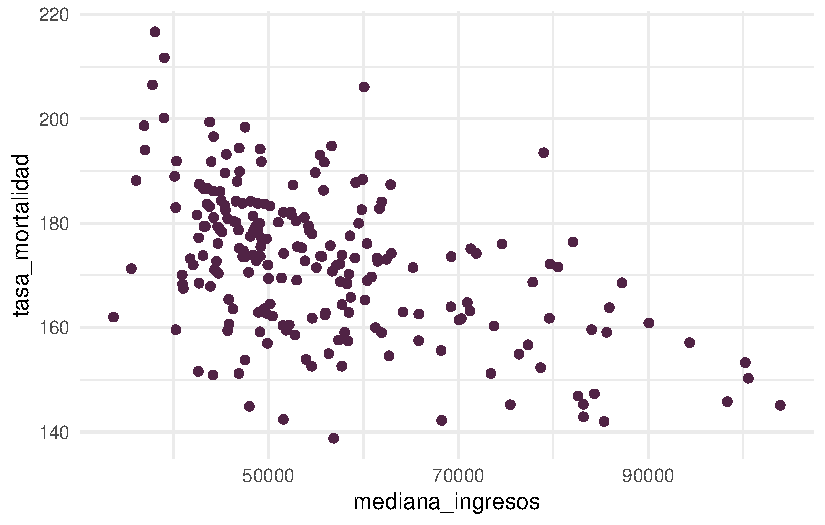
\includegraphics[width=0.85\linewidth,height=\textheight,keepaspectratio]{unidad_3/04_reg_lineal_files/figure-pdf/ej3-1.pdf}
\end{center}

Observamos en el gráfico una clara relación inversa entre las variables,
dado que los condados donde las personas tienen mayores ingresos la
mortalidad por cáncer es menor y viceversa. Podemos dibujar la recta de
regresión lineal sobre el diagrama de dispersión adicionando una capa
más al gráfico mediante \texttt{geom\_smooth()} e indicando
\texttt{method\ =\ "lm"} como método. Además de la recta se puede ver el
intervalo de confianza (zona gris alrededor de ella).

\begin{Shaded}
\begin{Highlighting}[]
\NormalTok{datos }\SpecialCharTok{|\textgreater{}}
  \FunctionTok{ggplot}\NormalTok{(}\AttributeTok{mapping =} \FunctionTok{aes}\NormalTok{(}\AttributeTok{x =}\NormalTok{ mediana\_ingresos, }\AttributeTok{y =}\NormalTok{ tasa\_mortalidad)) }\SpecialCharTok{+}

  \CommentTok{\# diagrama de dispersión}
  \FunctionTok{geom\_point}\NormalTok{(}\AttributeTok{color =} \StringTok{"\#502345"}\NormalTok{) }\SpecialCharTok{+}

  \CommentTok{\# añade línea de regresión}
  \FunctionTok{geom\_smooth}\NormalTok{(}\AttributeTok{method =} \StringTok{"lm"}\NormalTok{, }\AttributeTok{color =} \StringTok{"\#1B0D33"}\NormalTok{) }\SpecialCharTok{+}

  \CommentTok{\# cambia color de fondo}
  \FunctionTok{theme\_minimal}\NormalTok{()}
\end{Highlighting}
\end{Shaded}

\begin{center}
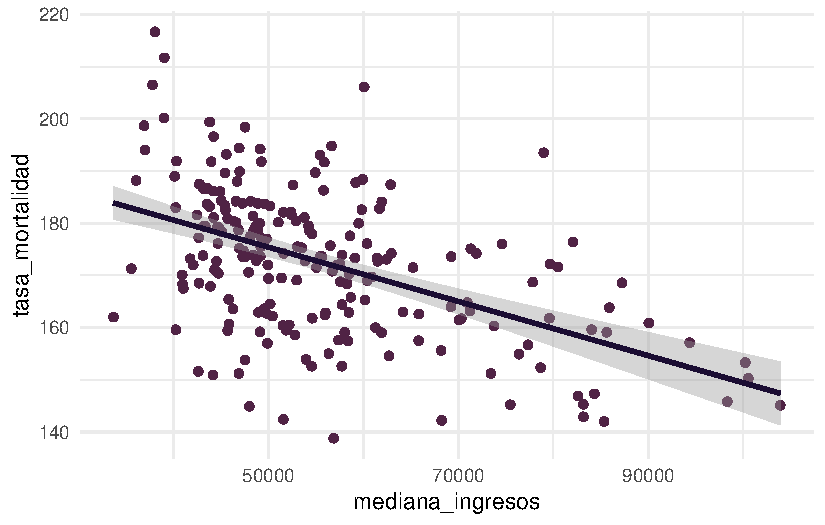
\includegraphics[width=0.85\linewidth,height=\textheight,keepaspectratio]{unidad_3/04_reg_lineal_files/figure-pdf/ej4-1.pdf}
\end{center}

Usaremos la función \texttt{cor()} para estimar la correlación entre las
dos variables:

\begin{Shaded}
\begin{Highlighting}[]
\FunctionTok{cor}\NormalTok{(datos}\SpecialCharTok{$}\NormalTok{mediana\_ingresos, datos}\SpecialCharTok{$}\NormalTok{tasa\_mortalidad, }\AttributeTok{method =} \StringTok{"pearson"}\NormalTok{)}
\end{Highlighting}
\end{Shaded}

\begin{verbatim}
[1] -0.5041398
\end{verbatim}

El valor es negativo, lo que confirma lo observado en la nube de puntos
anterior. Para poder descartar que esta \textbf{correlación negativa} se
debe al azar, debemos calcular su significancia:

\begin{Shaded}
\begin{Highlighting}[]
\FunctionTok{cor.test}\NormalTok{(datos}\SpecialCharTok{$}\NormalTok{mediana\_ingresos, datos}\SpecialCharTok{$}\NormalTok{tasa\_mortalidad)}
\end{Highlighting}
\end{Shaded}

\begin{verbatim}

    Pearson's product-moment correlation

data:  datos$mediana_ingresos and datos$tasa_mortalidad
t = -8.4795, df = 211, p-value = 3.938e-15
alternative hypothesis: true correlation is not equal to 0
95 percent confidence interval:
 -0.5980408 -0.3965857
sample estimates:
       cor 
-0.5041398 
\end{verbatim}

En este ejemplo \(p<0,05\), por lo tanto la correlación es
significativa.

La \textbf{homocedasticidad} implica que la varianza de los residuos se
mantiene aproximadamente constante a lo largo de los valores de la
variable independiente. Se puede evaluar gráficamente mediante la
dispersión de los residuos respecto a los valores ajustados o a través
de contrastes de hipótesis, como el \textbf{test de Breusch-Pagan}.

Finalmente, la \textbf{normalidad} de los residuos se puede evaluar
mediante el \textbf{test de Lilliefors}, disponible en el paquete
\texttt{nortest} (Gross y Ligges 2015):

\begin{Shaded}
\begin{Highlighting}[]
\FunctionTok{lillie.test}\NormalTok{(datos}\SpecialCharTok{$}\NormalTok{tasa\_mortalidad)}
\end{Highlighting}
\end{Shaded}

\begin{verbatim}

    Lilliefors (Kolmogorov-Smirnov) normality test

data:  datos$tasa_mortalidad
D = 0.042152, p-value = 0.4707
\end{verbatim}

También se puede verificar gráficamente con un \textbf{QQ plot}:

\begin{Shaded}
\begin{Highlighting}[]
\NormalTok{datos }\SpecialCharTok{|\textgreater{}}
  \FunctionTok{ggplot}\NormalTok{(}\AttributeTok{mapping =} \FunctionTok{aes}\NormalTok{(}\AttributeTok{sample =}\NormalTok{ tasa\_mortalidad)) }\SpecialCharTok{+}

  \CommentTok{\# añade qqplot}
  \FunctionTok{stat\_qq}\NormalTok{() }\SpecialCharTok{+}
  \FunctionTok{stat\_qq\_line}\NormalTok{() }\SpecialCharTok{+}

  \CommentTok{\# cambia nombres de los ejes X e Y}
  \FunctionTok{labs}\NormalTok{(}\AttributeTok{title =} \StringTok{"QQplot"}\NormalTok{, }\AttributeTok{x =} \StringTok{"Theoretical Quantiles"}\NormalTok{, }\AttributeTok{y =} \StringTok{"Sample Quantiles"}\NormalTok{) }\SpecialCharTok{+}

  \CommentTok{\# modifico color de fondo}
  \FunctionTok{theme\_minimal}\NormalTok{()}
\end{Highlighting}
\end{Shaded}

\begin{center}
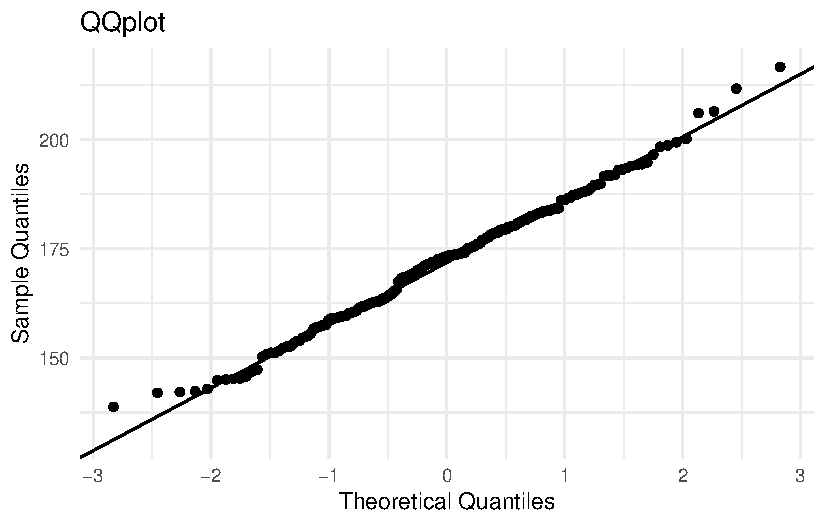
\includegraphics[width=0.85\linewidth,height=\textheight,keepaspectratio]{unidad_3/04_reg_lineal_files/figure-pdf/ej8-1.pdf}
\end{center}

Tanto el test de hipótesis como los gráficos de cuantiles nos informan
que las distribuciones de la variable dependiente cumple con el criterio
de ``normalidad''.

\subsection{Ajuste del modelo}\label{ajuste-del-modelo}

Como vimos
\hyperref[introducciuxf3n-al-modelado-estaduxedstico]{\textbf{anteriormente}},
la función \texttt{lm()} del paquete \texttt{stats} nos permite ajustar
modelos de regresión lineal:

\begin{Shaded}
\begin{Highlighting}[]
\FunctionTok{lm}\NormalTok{(tasa\_mortalidad }\SpecialCharTok{\textasciitilde{}}\NormalTok{ mediana\_ingresos, }\AttributeTok{data =}\NormalTok{ datos)}
\end{Highlighting}
\end{Shaded}

\begin{verbatim}

Call:
lm(formula = tasa_mortalidad ~ mediana_ingresos, data = datos)

Coefficients:
     (Intercept)  mediana_ingresos  
       201.41284          -0.00052  
\end{verbatim}

En este caso, \texttt{Intercept} representa el valor de
\texttt{mediana\_ingresos} cuando \texttt{tasa\_mortalidad} vale cero
(ordenada al origen) y el coeficiente de \texttt{mediana\_ingresos}
representa la pendiente de la recta.

Estos resultados obtenidos y aplicados en la fórmula del modelo simple
quedarían así:

\[
\operatorname{tasa mortalidad} = \alpha + \beta_{1}(\operatorname{mediana ingresos}) + \epsilon
\]

\[
\operatorname{tasa mortalidad} = 201.4128 + -0.0005*\operatorname{mediana ingresos} + \epsilon
\]

Guardamos el modelo como un objeto:

\begin{Shaded}
\begin{Highlighting}[]
\NormalTok{modelo }\OtherTok{\textless{}{-}} \FunctionTok{lm}\NormalTok{(tasa\_mortalidad }\SpecialCharTok{\textasciitilde{}}\NormalTok{ mediana\_ingresos, }\AttributeTok{data =}\NormalTok{ datos)}
\end{Highlighting}
\end{Shaded}

Podemos acceder a la salida del modelo mediante la función
\texttt{summary()}:

\begin{Shaded}
\begin{Highlighting}[]
\FunctionTok{summary}\NormalTok{(modelo)}
\end{Highlighting}
\end{Shaded}

\begin{verbatim}

Call:
lm(formula = tasa_mortalidad ~ mediana_ingresos, data = datos)

Residuals:
    Min      1Q  Median      3Q     Max 
-33.040  -8.210   1.093   7.637  35.932 

Coefficients:
                   Estimate Std. Error t value Pr(>|t|)    
(Intercept)       2.014e+02  3.521e+00  57.200  < 2e-16 ***
mediana_ingresos -5.200e-04  6.133e-05  -8.479 3.94e-15 ***
---
Signif. codes:  0 '***' 0.001 '**' 0.01 '*' 0.05 '.' 0.1 ' ' 1

Residual standard error: 12.32 on 211 degrees of freedom
Multiple R-squared:  0.2542,    Adjusted R-squared:  0.2506 
F-statistic:  71.9 on 1 and 211 DF,  p-value: 3.938e-15
\end{verbatim}

La asociación entre la tasa de mortalidad por cáncer y la mediana de
ingresos es estadísticamente significativa (\(p < 0.001\)).

Todos los ajustes de modelos lineales que produce la función
\texttt{lm()} tienen la forma de una lista.La manera de conocer su clase
es \texttt{class()} y su estructura mediante \texttt{str()}

\begin{Shaded}
\begin{Highlighting}[]
\FunctionTok{class}\NormalTok{(modelo)}
\end{Highlighting}
\end{Shaded}

\begin{verbatim}
[1] "lm"
\end{verbatim}

\begin{Shaded}
\begin{Highlighting}[]
\FunctionTok{str}\NormalTok{(modelo)}
\end{Highlighting}
\end{Shaded}

\begin{verbatim}
List of 12
 $ coefficients : Named num [1:2] 201.41284 -0.00052
  ..- attr(*, "names")= chr [1:2] "(Intercept)" "mediana_ingresos"
 $ residuals    : Named num [1:213] 12.3 -2.68 -9.49 2.28 -17.11 ...
  ..- attr(*, "names")= chr [1:213] "1" "2" "3" "4" ...
 $ effects      : Named num [1:213] -2516.47 104.46 -10.27 1.26 -17.89 ...
  ..- attr(*, "names")= chr [1:213] "(Intercept)" "mediana_ingresos" "" "" ...
 $ rank         : int 2
 $ fitted.values: Named num [1:213] 170 171 172 179 172 ...
  ..- attr(*, "names")= chr [1:213] "1" "2" "3" "4" ...
 $ assign       : int [1:2] 0 1
 $ qr           :List of 5
  ..$ qr   : num [1:213, 1:2] -14.5945 0.0685 0.0685 0.0685 0.0685 ...
  .. ..- attr(*, "dimnames")=List of 2
  .. .. ..$ : chr [1:213] "1" "2" "3" "4" ...
  .. .. ..$ : chr [1:2] "(Intercept)" "mediana_ingresos"
  .. ..- attr(*, "assign")= int [1:2] 0 1
  ..$ qraux: num [1:2] 1.07 1.01
  ..$ pivot: int [1:2] 1 2
  ..$ tol  : num 1e-07
  ..$ rank : int 2
  ..- attr(*, "class")= chr "qr"
 $ df.residual  : int 211
 $ xlevels      : Named list()
 $ call         : language lm(formula = tasa_mortalidad ~ mediana_ingresos, data = datos)
 $ terms        :Classes 'terms', 'formula'  language tasa_mortalidad ~ mediana_ingresos
  .. ..- attr(*, "variables")= language list(tasa_mortalidad, mediana_ingresos)
  .. ..- attr(*, "factors")= int [1:2, 1] 0 1
  .. .. ..- attr(*, "dimnames")=List of 2
  .. .. .. ..$ : chr [1:2] "tasa_mortalidad" "mediana_ingresos"
  .. .. .. ..$ : chr "mediana_ingresos"
  .. ..- attr(*, "term.labels")= chr "mediana_ingresos"
  .. ..- attr(*, "order")= int 1
  .. ..- attr(*, "intercept")= int 1
  .. ..- attr(*, "response")= int 1
  .. ..- attr(*, ".Environment")=<environment: R_GlobalEnv> 
  .. ..- attr(*, "predvars")= language list(tasa_mortalidad, mediana_ingresos)
  .. ..- attr(*, "dataClasses")= Named chr [1:2] "numeric" "numeric"
  .. .. ..- attr(*, "names")= chr [1:2] "tasa_mortalidad" "mediana_ingresos"
 $ model        :'data.frame':  213 obs. of  2 variables:
  ..$ tasa_mortalidad : num [1:213] 183 169 163 182 155 ...
  ..$ mediana_ingresos: num [1:213] 59831 57556 56008 42491 56353 ...
  ..- attr(*, "terms")=Classes 'terms', 'formula'  language tasa_mortalidad ~ mediana_ingresos
  .. .. ..- attr(*, "variables")= language list(tasa_mortalidad, mediana_ingresos)
  .. .. ..- attr(*, "factors")= int [1:2, 1] 0 1
  .. .. .. ..- attr(*, "dimnames")=List of 2
  .. .. .. .. ..$ : chr [1:2] "tasa_mortalidad" "mediana_ingresos"
  .. .. .. .. ..$ : chr "mediana_ingresos"
  .. .. ..- attr(*, "term.labels")= chr "mediana_ingresos"
  .. .. ..- attr(*, "order")= int 1
  .. .. ..- attr(*, "intercept")= int 1
  .. .. ..- attr(*, "response")= int 1
  .. .. ..- attr(*, ".Environment")=<environment: R_GlobalEnv> 
  .. .. ..- attr(*, "predvars")= language list(tasa_mortalidad, mediana_ingresos)
  .. .. ..- attr(*, "dataClasses")= Named chr [1:2] "numeric" "numeric"
  .. .. .. ..- attr(*, "names")= chr [1:2] "tasa_mortalidad" "mediana_ingresos"
 - attr(*, "class")= chr "lm"
\end{verbatim}

La función \texttt{tbl\_regression()} del paquete \texttt{gtsummary}
(Sjoberg et~al. 2021), nos permite generar una tabla con los
coeficientes del modelo. El nivel de confianza puede ajustarse con el
argumento \texttt{conf.level} y el argumento \texttt{intercept} muestra
u oculta el intercepto:

\begin{Shaded}
\begin{Highlighting}[]
\FunctionTok{tbl\_regression}\NormalTok{(modelo, }\AttributeTok{intercept =}\NormalTok{ T, }\AttributeTok{conf.level =}\NormalTok{ .}\DecValTok{95}\NormalTok{)}
\end{Highlighting}
\end{Shaded}

\begin{table}
\fontsize{12.0pt}{14.0pt}\selectfont
\begin{tabular*}{\linewidth}{@{\extracolsep{\fill}}lccc}
\toprule
\textbf{Characteristic} & \textbf{Beta} & \textbf{95\% CI} & \textbf{p-value} \\ 
\midrule\addlinespace[2.5pt]
(Intercept) & 201 & 194, 208 & <0.001 \\ 
mediana\_ingresos & 0.00 & 0.00, 0.00 & <0.001 \\ 
\bottomrule
\end{tabular*}
\begin{minipage}{\linewidth}
\vspace{.05em}
Abbreviation: CI = Confidence Interval\\
\end{minipage}
\end{table}

\subsection{Residuales}\label{residuales}

El \textbf{residuo} o \textbf{residual} de una estimación se define como
la diferencia entre el valor observado y el valor predicho por el modelo
de regresión. Son fundamentales para evaluar la bondad de ajuste y
verificar los supuestos básicos de los modelos lineales. Para resumir el
conjunto de residuales, se pueden emplear dos enfoques:

\begin{enumerate}
\def\labelenumi{\arabic{enumi}.}
\item
  La \textbf{sumatoria del valor absoluto} de cada residual.
\item
  La \textbf{sumatoria del cuadrado} de cada residual (\textbf{RSS,}
  \emph{Residual Sum of Squares}), basada en el método de los mínimos
  cuadrados, amplifica las desviaciones extremas y permite minimizar
  errores en la estimación de parámetros.
\end{enumerate}

Los residuales se almacenan en el objeto de regresión y pueden
visualizarse mediante:

\begin{Shaded}
\begin{Highlighting}[]
\FunctionTok{resid}\NormalTok{(modelo)}
\end{Highlighting}
\end{Shaded}

Cuanto mayor sea la \textbf{sumatoria de los cuadrados de los
residuales}, menor será la precisión con la que el modelo predice el
valor de la variable dependiente a partir de la variable predictora.

Un análisis gráfico resulta muy útil para evaluar los supuestos del
modelo. Aplicando la función \texttt{plot()} al objeto de regresión:

\begin{Shaded}
\begin{Highlighting}[]
\FunctionTok{par}\NormalTok{(}\AttributeTok{mfrow =} \FunctionTok{c}\NormalTok{(}\DecValTok{2}\NormalTok{, }\DecValTok{2}\NormalTok{))}
\FunctionTok{plot}\NormalTok{(modelo)}
\end{Highlighting}
\end{Shaded}

\begin{center}
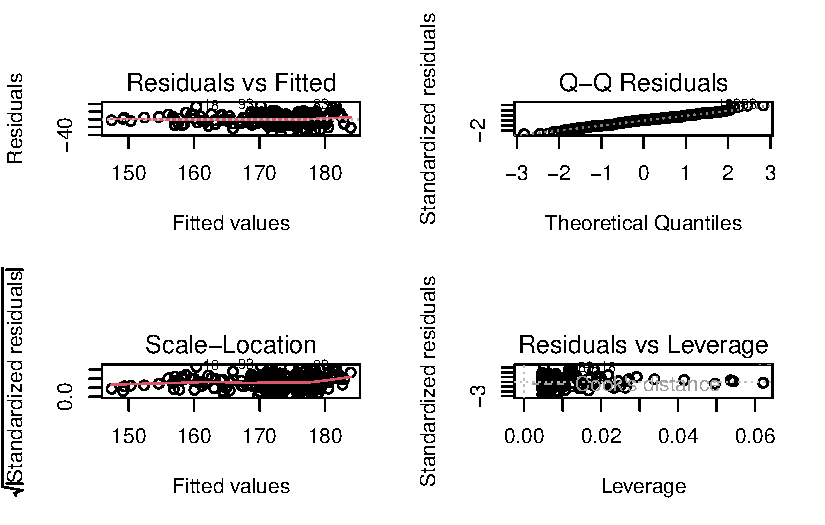
\includegraphics[width=0.85\linewidth,height=\textheight,keepaspectratio]{unidad_3/04_reg_lineal_files/figure-pdf/ej15-1.pdf}
\end{center}

Esta función genera cuatro gráficos automáticos:

\begin{itemize}
\item
  \texttt{Residuals\ vs\ Fitted}\textbf{:} Permite evaluar la
  \textbf{linealidad}. La línea roja debería ser lo más horizontal
  posible y sin curvaturas pronunciadas. Si hay curvatura, podría
  indicar la necesidad de un término no lineal (cuadrático, logarítmico,
  etc.) o la omisión de una variable importante en el modelo.
\item
  \texttt{Normal\ Q-Q}\textbf{:} Evalúa la \textbf{normalidad} de los
  residuos. Los puntos deberían ajustarse a la diagonal. Desviaciones
  importantes sugieren un incumplimiento del supuesto de normalidad.
\item
  \texttt{Scale-Location}\textbf{:} Indica si los residuos se
  distribuyen uniformemente a lo largo del rango de los predictores,
  verificando la \textbf{homocedasticidad}. Una línea aproximadamente
  horizontal con puntos dispersos de manera aleatoria es una buena
  señal.
\item
  \texttt{Residuals\ vs\ Leverage}\textbf{:} Ayuda a identificar
  \textbf{valores influyentes}. Un punto extremo no necesariamente es
  influyente, pero aquellos fuera de las líneas rojas punteadas (altas
  puntuaciones de distancia de Cook) pueden estar afectando
  considerablemente el modelo.
\end{itemize}

Otra opción para evaluar gráficamente los supuestos del modelo es la
función \texttt{check\_model()} del paquete \texttt{performance} , el
cual forma parte del ecosistema \texttt{easystats} (Lüdecke et~al.
2022):

\begin{Shaded}
\begin{Highlighting}[]
\FunctionTok{check\_model}\NormalTok{(modelo)}
\end{Highlighting}
\end{Shaded}

Podemos elegir que gráficos visualizar usando el argumento
\texttt{check}:

\begin{Shaded}
\begin{Highlighting}[]
\FunctionTok{check\_model}\NormalTok{(}
\NormalTok{  modelo,}
  \AttributeTok{check =} \FunctionTok{c}\NormalTok{(}\StringTok{"normality"}\NormalTok{, }\StringTok{"qq"}\NormalTok{, }\StringTok{"linearity"}\NormalTok{, }\StringTok{"homogeneity"}\NormalTok{, }\StringTok{"outliers"}\NormalTok{)}
\NormalTok{)}
\end{Highlighting}
\end{Shaded}

Para evaluar la linealidad se puede aplicar el test RESET de Ramsey,
mediante la función \texttt{resettest()} del paquete \texttt{lmtest}
(Zeileis y Hothorn 2002):

\begin{Shaded}
\begin{Highlighting}[]
\FunctionTok{resettest}\NormalTok{(modelo)}
\end{Highlighting}
\end{Shaded}

\begin{verbatim}

    RESET test

data:  modelo
RESET = 0.82653, df1 = 2, df2 = 209, p-value = 0.439
\end{verbatim}

La hipótesis nula indica que las variables se relacionan de forma
lineal; un \(p<0,05\) sugiere lo contrario. En nuestro modelo, el valor
\emph{p} de 0.439 respalda la suposición de linealidad.

Otro supuesto fundamental es que los residuales deben distribuirse de
forma normal (con media 0). Además del QQ-plot, se puede aplicar el test
de Lilliefors:

\begin{Shaded}
\begin{Highlighting}[]
\FunctionTok{lillie.test}\NormalTok{(modelo}\SpecialCharTok{$}\NormalTok{residuals)}
\end{Highlighting}
\end{Shaded}

\begin{verbatim}

    Lilliefors (Kolmogorov-Smirnov) normality test

data:  modelo$residuals
D = 0.05804, p-value = 0.07821
\end{verbatim}

Con un \emph{p}-valor de 0.078 se confirma la normalidad.

El test de Breusch-Pagan, implementado en \texttt{lmtest} y
\texttt{performance}, evalúa si la varianza de los residuos es
constante. Parte de la hipótesis nula de \textbf{homocedasticidad} o
varianza constante en las perturbaciones y la enfrenta a la alternativa
de varianza variable, por lo que es válido decir que cumple con el
supuesto de homocedasticidad si el valor \(p>0,05\):

\begin{Shaded}
\begin{Highlighting}[]
\CommentTok{\# paquete lmtest}
\FunctionTok{bptest}\NormalTok{(modelo)}
\end{Highlighting}
\end{Shaded}

\begin{verbatim}

    studentized Breusch-Pagan test

data:  modelo
BP = 2.5078, df = 1, p-value = 0.1133
\end{verbatim}

\begin{Shaded}
\begin{Highlighting}[]
\CommentTok{\# paquete performance}
\FunctionTok{check\_heteroscedasticity}\NormalTok{(modelo)}
\end{Highlighting}
\end{Shaded}

\begin{verbatim}
OK: Error variance appears to be homoscedastic (p = 0.087).
\end{verbatim}

Incluso cuando el modelo cumple todos los supuestos, es importante
identificar observaciones atípicas o de alto \emph{leverage}, ya que
podrían condicionar el ajuste. Los valores atípicos u \emph{outliers}
son observaciones que no se ajustan bien al modelo, con residuos
excesivamente grandes. Por otro lado, los puntos con alto
\emph{leverage} tienen valores extremos en los predictores, lo que los
hace potencialmente influyentes.

Para ello se pueden analizar los residuales estandarizados y los
residuales estudentizados. Los \textbf{residuales estandarizados} se
obtienen normalizando los residuales por su desviación estándar. Esta
aproximación permite identificar valores atípicos que se alejan más de
\(\pm3\) desviaciones estándar. Sin embargo, si un \emph{outlier}
influye lo suficiente en el modelo como para atraer la línea de
regresión, su residual podría ser pequeño y pasar desapercibido. Una
alternativa más robusta es utilizar los \textbf{residuales
estudentizados}. Se trata de un proceso iterativo en el que se va
excluyendo cada vez una observación \(i\) distinta y se reajusta el
modelo con las \(n-1\) restantes. En cada proceso de exclusión y
reajuste se calcula la diferencia (\(d_i\)) entre el valor predicho para
\(i\) habiendo y sin haber excluido esa observación. Finalmente, se
normalizan las diferencias \(d_i\) . Aquellos valores \(d_i\) cuyo
residual estudentizado supera \(\pm 3\) suelen considerarse
significativos.

Estos dos procesos sobre los residuales se pueden calcular en R mediante
las funciones \texttt{rstandar()} y \texttt{rstudent()}:

\begin{Shaded}
\begin{Highlighting}[]
\CommentTok{\# Creación del dataset de residuales}
\NormalTok{residuales }\OtherTok{\textless{}{-}} \FunctionTok{tibble}\NormalTok{(}
  \AttributeTok{residuales =} \FunctionTok{residuals}\NormalTok{(modelo),}
  \AttributeTok{resid\_normalizados =} \FunctionTok{rstandard}\NormalTok{(modelo),}
  \AttributeTok{resid\_estudentizados =} \FunctionTok{rstudent}\NormalTok{(modelo)}
\NormalTok{)}
\end{Highlighting}
\end{Shaded}

Podemos visualizar la comparación de estos residuales mediante un
\emph{boxplot} usando \emph{facets}:

\begin{Shaded}
\begin{Highlighting}[]
\NormalTok{residuales }\SpecialCharTok{|\textgreater{}}

  \CommentTok{\# Pasa a formato long}
  \FunctionTok{pivot\_longer}\NormalTok{(}\AttributeTok{cols =} \FunctionTok{everything}\NormalTok{(), }\AttributeTok{names\_to =} \StringTok{"tipo"}\NormalTok{) }\SpecialCharTok{|\textgreater{}}

  \CommentTok{\# Genera gráfico}
  \FunctionTok{ggplot}\NormalTok{(}\AttributeTok{mapping =} \FunctionTok{aes}\NormalTok{(}\AttributeTok{y =}\NormalTok{ value, }\AttributeTok{fill =}\NormalTok{ tipo)) }\SpecialCharTok{+}

  \FunctionTok{geom\_boxplot}\NormalTok{() }\SpecialCharTok{+}

  \FunctionTok{scale\_fill\_scico\_d}\NormalTok{() }\SpecialCharTok{+}

  \FunctionTok{facet\_wrap}\NormalTok{(}\SpecialCharTok{\textasciitilde{}}\NormalTok{tipo, }\AttributeTok{scales =} \StringTok{"free\_y"}\NormalTok{) }\SpecialCharTok{+} \CommentTok{\# subdivide en facets}

  \FunctionTok{theme\_minimal}\NormalTok{()}
\end{Highlighting}
\end{Shaded}

\begin{center}
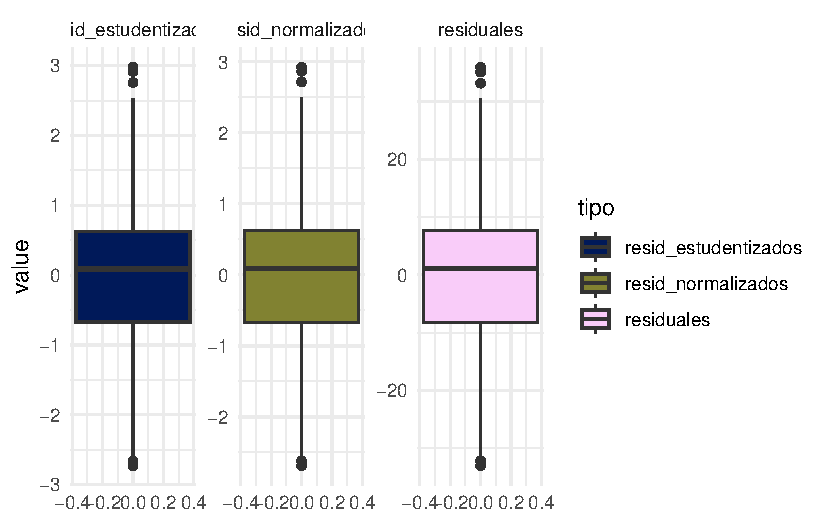
\includegraphics[width=0.85\linewidth,height=\textheight,keepaspectratio]{unidad_3/04_reg_lineal_files/figure-pdf/ej22-1.pdf}
\end{center}

Si encontramos residuales con valores absolutos superiores a 3 en el
gráfico de residuales estudentizados, es recomendable investigarlos más
a fondo. Podemos identificarlos con:

\begin{Shaded}
\begin{Highlighting}[]
\FunctionTok{table}\NormalTok{(}\FunctionTok{rstudent}\NormalTok{(modelo) }\SpecialCharTok{\textgreater{}} \DecValTok{3}\NormalTok{)}
\end{Highlighting}
\end{Shaded}

\begin{verbatim}

FALSE 
  213 
\end{verbatim}

Para evaluar la influencia de observaciones, se utiliza la
\textbf{distancia de Cook}, que combina la magnitud del residual y el
\emph{leverage}. Valores superiores a 1 se consideran generalmente
influyentes. Esto se puede visualizar mediante:

\begin{Shaded}
\begin{Highlighting}[]
\FunctionTok{plot}\NormalTok{(modelo, }\AttributeTok{which =} \DecValTok{5}\NormalTok{)}
\end{Highlighting}
\end{Shaded}

\begin{center}
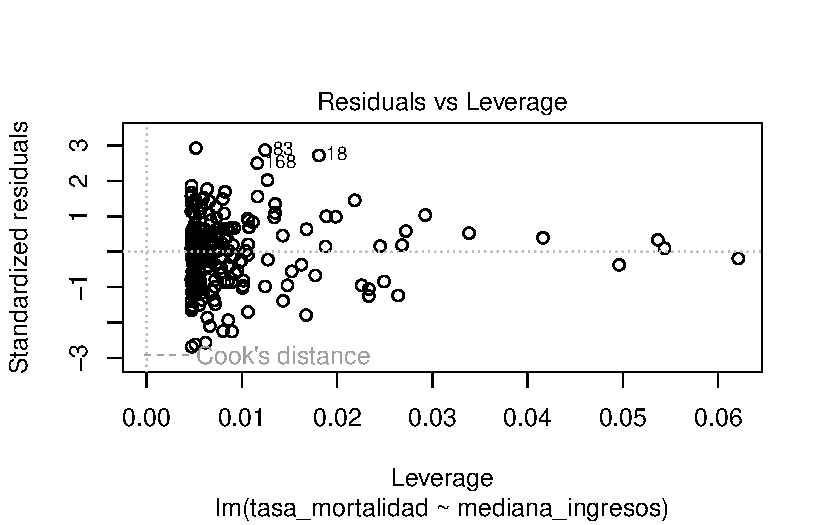
\includegraphics[width=0.85\linewidth,height=\textheight,keepaspectratio]{unidad_3/04_reg_lineal_files/figure-pdf/ej24-1.pdf}
\end{center}

Al observar el gráfico, se debe prestar especial atención a los puntos
situados en las esquinas superior e inferior, es decir, aquellos que
aparecen fuera de las líneas discontinuas rojas. Estos puntos suelen
presentar altas puntuaciones en la distancia de Cook, lo que indica que
pueden influir significativamente en los resultados de la regresión.

Además, el paquete \texttt{performance} incluye la función
\texttt{check\_outliers()} para detectar valores atípicos según su
distancia de Cook:

\begin{Shaded}
\begin{Highlighting}[]
\FunctionTok{check\_outliers}\NormalTok{(modelo)}
\end{Highlighting}
\end{Shaded}

\begin{verbatim}
OK: No outliers detected.
- Based on the following method and threshold: cook (0.7).
- For variable: (Whole model)
\end{verbatim}

En el ejemplo analizado, no se identificaron valores influyentes
evidentes. Sin embargo, si se detecta alguna observación fuera de estos
límites, es recomendable estudiarla de forma individual para determinar,
por ejemplo, si su elevada influencia se debe a un error de registro. En
tal caso podremos eliminar la observación (o corregirla) y analizar los
casos restantes. Pero si el dato es correcto, quizás sea diferente de
las otras observaciones y encontrar las causas de este fenómeno puede
llegar a ser la parte más interesante del análisis. Por supuesto que
todo esto dependerá del contexto del problema que uno esta estudiando.

\subsection{Bondad de ajuste del
modelo}\label{bondad-de-ajuste-del-modelo}

Una vez ajustado un modelo, es necesario verificar su eficiencia, ya
que, aun siendo la línea que mejor se ajusta a las observaciones entre
todas las posibles, el modelo puede resultar inadecuado. Entre las
medidas más utilizadas para evaluar la calidad del ajuste se encuentran
el error estándar de los residuales, el test \(F\) y el coeficiente de
determinación \(R^2\). Estos valores aparecen al final de la salida de
la función \texttt{summary()}, donde se pueden identificar el RSE
(\emph{Residual Standard Error}), el \(R^2\) (\emph{Multiple R-squared})
y el \(R^2\) ajustado (\emph{Adjusted R-squared}).

Podemos acceder al valor de \(R^2\) del modelo usando la función
\texttt{r2()} del paquete \texttt{performance}:

\begin{Shaded}
\begin{Highlighting}[]
\FunctionTok{r2}\NormalTok{(modelo)}
\end{Highlighting}
\end{Shaded}

\begin{verbatim}
# R2 for Linear Regression
       R2: 0.254
  adj. R2: 0.251
\end{verbatim}

El \(R^2\) oscila entre 0 y 1, de modo que valores cercanos a 1 indican
un buen ajuste del modelo lineal a los datos. Por otro lado, el \(R^2\)
ajustado penaliza la inclusión de variables independientes poco
relevantes en la explicación de la variable dependiente, razón por la
cual su valor es menor o igual al \(R^2\). En nuestro ejemplo los
valores de \(R^2\) obtenidos nos indican que el modelo lineal simple no
se ajusta demasiado bien a los datos. Esto significa que solamente un
25.1\,\% de la variación en la tasa de mortalidad por cáncer se explica
únicamente por la mediana de ingresos como variable explicativa; el
restante 74.9\,\% no se explica, lo que sugiere que agregar otras
variables independientes podría mejorar el ajuste y, por ende, la
confiabilidad de las predicciones.

La salida de \texttt{summary()} también incluye un estadístico \(F\) de
Snedecor y su \(p\)\emph{-}valor correspondiente, que se utilizan en el
contraste ómnibus para evaluar, de forma global, la idoneidad del
modelo. En nuestro ejemplo, \(p>0,05\), por lo que, al 95\,\% de
confianza, se rechaza la hipótesis nula y se concluye que el modelo
lineal es adecuado para el conjunto de datos. Cabe mencionar que, cuando
el modelo de regresión tiene una única variable explicativa, este
contraste es equivalente al contraste del parámetro \(\beta_1​\).

Otra forma de verificar de manera independiente la significación del
modelo es mediante la función \texttt{anova()}, que plantea el contraste
de la regresión mediante el \href{05_anova.qmd}{\textbf{análisis de la
varianza}}:

\begin{Shaded}
\begin{Highlighting}[]
\FunctionTok{anova}\NormalTok{(modelo)}
\end{Highlighting}
\end{Shaded}

\begin{verbatim}
Analysis of Variance Table

Response: tasa_mortalidad
                  Df Sum Sq Mean Sq F value    Pr(>F)    
mediana_ingresos   1  10912 10911.8  71.901 3.938e-15 ***
Residuals        211  32021   151.8                      
---
Signif. codes:  0 '***' 0.001 '**' 0.01 '*' 0.05 '.' 0.1 ' ' 1
\end{verbatim}

La tabla de análisis de varianza muestra resultados coherentes con el
bloque final de \texttt{summary(modelo)}, presentando un valor \(F\) de
71.9 y un \(p\)-valor significativo.

\subsection{Interpretación de
resultados}\label{interpretaciuxf3n-de-resultados}

Se realizó una regresión lineal simple para analizar la relación entre
la mediana de ingresos y la tasa de mortalidad por cáncer en 174
condados de la Costa Este de Estados Unidos. El diagrama de dispersión
mostró una relación lineal negativa moderada entre ambas variables, lo
que se confirmó con un coeficiente de correlación de Pearson de\\
-0.5. Además, el análisis de regresión reveló que la relación es
estadísticamente significativa (t = -8.48, \emph{p} = 0).

El coeficiente de pendiente para la mediana de ingresos fue de\\
0, lo que indica que, por cada unidad de incremento en la mediana de
ingresos, la tasa de mortalidad por cáncer disminuye aproximadamente en
0,05 puntos porcentuales. El \(R^2\) del modelo muestra que el 25.1\,\%
de la variación en la tasa de mortalidad se explica únicamente con esta
variable, lo que sugiere la existencia de otros factores que también
influyen en la mortalidad por cáncer.

Finalmente, la gráfica de dispersión de los valores pronosticados
estandarizados frente a los residuos estandarizados evidenció que se
cumplen los supuestos de homogeneidad de varianza y linealidad, y que
los residuos se distribuyen de forma aproximadamente normal. Se
cumplieron todos los presupuestos necesarios para validar la regresión y
no se encontraron valores atípicos influyentes.

Ballester Díez y Tenías Burillo (2003)

Daniel (2002)

Hernández-Ávila (2011)

Weisberg (2005)

Royo-Bordonada et~al. (2009)

\section*{Referencias}\label{referencias-14}
\addcontentsline{toc}{section}{Referencias}

\markright{Referencias}

\chapter{Análisis de la varianza
(ANOVA)}\label{anuxe1lisis-de-la-varianza-anova}

\section{Introducción}\label{introducciuxf3n-14}

El análisis de varianza (ANOVA) es una extensión del modelo lineal
general que se utiliza para comparar las medias de una variable
dependiente continua (\(Y\)) entre diferentes niveles de una variable
explicativa categórica (\(X\)), que debe tener al menos tres niveles.

La hipótesis nula (\(H_0\)) del test estadístico establece que las
medias de la variable dependiente son iguales en todos los grupos,
mientras que la hipótesis alternativa (\(H_1\)) plantea que al menos dos
medias difieren significativamente:

\begin{itemize}
\item
  H0: \$\mu\_1 = \mu\_2 = \ldots{} = \mu\_i \$
\item
  H\_1: al menos una \$\mu\_i \not= \mu\_j \$
\end{itemize}

Por lo tanto, el ANOVA permite comparar múltiples medias, pero lo hace
analizando la variabilidad entre y dentro de los grupos.

La variabilidad total se descompone en dos componentes:

\begin{itemize}
\item
  \textbf{Intervarianza (SSB):} Variabilidad entre los grupos.
\item
  \textbf{Intravarianza (SSE):} Variabilidad dentro de los grupos.
\end{itemize}

El estadístico \(F\) del ANOVA, que sigue una distribución F de
Fisher-Snedecor, compara estas dos fuentes de variabilidad:

\[
F = \frac{SSB/(k-1)}{SSE/(n-k)}
\]

donde:

\begin{itemize}
\item
  \(k\): el número de grupos.
\item
  \(n\): número total de observaciones.
\end{itemize}

Si se cumple H0, el estadístico \(F\) tiende a 1, ya que las varianzas
entre y dentro de los grupos son similares. Si las medias difieren
significativamente, la intervarianza será mayor que la intravarianza,
resultando en valores de \(F\) superiores a 1.

\section{ANOVA de un factor o de una
vía}\label{anova-de-un-factor-o-de-una-vuxeda}

El ANOVA de una vía puede considerare como una extensión de los
\emph{t-test} independientes para comparar más de dos grupos de un
factor. En este contexto, factor se refiere a la variable categórica que
define los grupos.

Para que los resultados del ANOVA sean válidos, deben cumplirse los
siguientes supuestos:

\begin{itemize}
\item
  \textbf{Aleatoriedad:} Las observaciones deben ser aleatorias.
\item
  \textbf{Independencia:} Las observaciones entre grupos deben ser
  independientes.
\item
  \textbf{Variable dependiente:} Cuantitativa continua.
\item
  \textbf{Variable explicativa:} Categórica con más de dos niveles.
\item
  \textbf{Normalidad:} La distribución de la variable dependiente dentro
  de cada grupo debe ser normal.
\item
  \textbf{Homocedasticidad:} Las varianzas de los grupos deben ser
  homogéneas.
\end{itemize}

\section{Ejemplo práctico en R}\label{ejemplo-pruxe1ctico-en-r-6}

Nuevamente vamos a trabajar con el conjunto de datos
``\texttt{cancer\_USA.txt}'', que contiene información sobre la tasa de
mortalidad por cáncer (por 100.000 habitantes) en distintos condados de
la Costa Este de Estados Unidos. Nuestro objetivo será analizar la
relación entre la tasa de mortalidad (\texttt{tasa\_mortalidad}) y el
estado de residencia (\texttt{estado}).

Comenzaremos por cargar los paquetes necesarios:

\begin{Shaded}
\begin{Highlighting}[]
\CommentTok{\# tablas salida del modelo}
\FunctionTok{library}\NormalTok{(gtsummary)}

\CommentTok{\# chequeo de supuestos}
\FunctionTok{library}\NormalTok{(easystats)}
\FunctionTok{library}\NormalTok{(nortest)}
\FunctionTok{library}\NormalTok{(pwr)}

\CommentTok{\# comparación de medias}
\FunctionTok{library}\NormalTok{(emmeans)}

\CommentTok{\# análisis exploratorio}
\FunctionTok{library}\NormalTok{(skimr)}
\FunctionTok{library}\NormalTok{(dlookr)}

\CommentTok{\# paletas de colores aptas daltonismo}
\FunctionTok{library}\NormalTok{(scico)}

\CommentTok{\# manejo de datos}
\FunctionTok{library}\NormalTok{(janitor)}
\FunctionTok{library}\NormalTok{(tidyverse)}
\end{Highlighting}
\end{Shaded}

Cargamos y exploramos los datos:

\begin{Shaded}
\begin{Highlighting}[]
\CommentTok{\# Carga datos}
\NormalTok{datos }\OtherTok{\textless{}{-}} \FunctionTok{read\_csv2}\NormalTok{(}\StringTok{"datos/cancer\_USA.txt"}\NormalTok{)}

\CommentTok{\# Explora datos}
\FunctionTok{glimpse}\NormalTok{(datos)}
\end{Highlighting}
\end{Shaded}

\begin{verbatim}
Rows: 213
Columns: 10
$ condado            <chr> "Belknap County", "Carroll County", "Cheshire Count~
$ estado             <chr> "New Hampshire", "New Hampshire", "New Hampshire", ~
$ tasa_mortalidad    <dbl> 182.6, 168.8, 162.8, 181.6, 155.0, 163.2, 173.1, 17~
$ mediana_edad       <dbl> 46.1, 50.3, 42.0, 48.1, 41.9, 40.1, 42.6, 43.5, 37.~
$ mediana_edad_cat   <chr> "45+ años", "45+ años", "36-39 años", "45+ años", "~
$ mediana_ingresos   <dbl> 59831, 57556, 56008, 42491, 56353, 71233, 62429, 79~
$ pct_pobreza        <dbl> 10.0, 10.7, 11.8, 14.9, 11.6, 8.7, 9.5, 6.1, 11.8, ~
$ pct_salud_publica  <dbl> 16.8, 13.4, 12.7, 22.5, 14.0, 12.7, 13.1, 9.0, 12.4~
$ pct_sec_incompleta <dbl> 15.4, 14.8, 6.1, 13.2, 6.6, 12.9, 10.9, 13.5, 6.1, ~
$ pct_desempleo      <dbl> 5.3, 5.8, 6.1, 6.9, 5.0, 5.9, 5.2, 5.6, 6.5, 5.8, 1~
\end{verbatim}

La base de datos tiene observaciones y variables. La variable
dependiente es \texttt{tasa\_mortalidad}, mientras que \texttt{estado}
es nuestra variable explicativa, categórica con 9 niveles.

Exploremos más en profundidad la estructura de los datos usando la
función \texttt{skim()} del paquete \texttt{skimr}:

\begin{Shaded}
\begin{Highlighting}[]
\CommentTok{\# Resumen de los datos}
\FunctionTok{skim}\NormalTok{(datos)}
\end{Highlighting}
\end{Shaded}

\begin{longtable}[]{@{}ll@{}}
\caption{Data summary}\tabularnewline
\toprule\noalign{}
\endfirsthead
\endhead
\bottomrule\noalign{}
\endlastfoot
Name & datos \\
Number of rows & 213 \\
Number of columns & 10 \\
\_\_\_\_\_\_\_\_\_\_\_\_\_\_\_\_\_\_\_\_\_\_\_ & \\
Column type frequency: & \\
character & 3 \\
numeric & 7 \\
\_\_\_\_\_\_\_\_\_\_\_\_\_\_\_\_\_\_\_\_\_\_\_\_ & \\
Group variables & None \\
\end{longtable}

\textbf{Variable type: character}

{\def\LTcaptype{none} % do not increment counter
\begin{longtable}[]{@{}
  >{\raggedright\arraybackslash}p{(\linewidth - 14\tabcolsep) * \real{0.2267}}
  >{\raggedleft\arraybackslash}p{(\linewidth - 14\tabcolsep) * \real{0.1333}}
  >{\raggedleft\arraybackslash}p{(\linewidth - 14\tabcolsep) * \real{0.1867}}
  >{\raggedleft\arraybackslash}p{(\linewidth - 14\tabcolsep) * \real{0.0533}}
  >{\raggedleft\arraybackslash}p{(\linewidth - 14\tabcolsep) * \real{0.0533}}
  >{\raggedleft\arraybackslash}p{(\linewidth - 14\tabcolsep) * \real{0.0800}}
  >{\raggedleft\arraybackslash}p{(\linewidth - 14\tabcolsep) * \real{0.1200}}
  >{\raggedleft\arraybackslash}p{(\linewidth - 14\tabcolsep) * \real{0.1467}}@{}}
\toprule\noalign{}
\begin{minipage}[b]{\linewidth}\raggedright
skim\_variable
\end{minipage} & \begin{minipage}[b]{\linewidth}\raggedleft
n\_missing
\end{minipage} & \begin{minipage}[b]{\linewidth}\raggedleft
complete\_rate
\end{minipage} & \begin{minipage}[b]{\linewidth}\raggedleft
min
\end{minipage} & \begin{minipage}[b]{\linewidth}\raggedleft
max
\end{minipage} & \begin{minipage}[b]{\linewidth}\raggedleft
empty
\end{minipage} & \begin{minipage}[b]{\linewidth}\raggedleft
n\_unique
\end{minipage} & \begin{minipage}[b]{\linewidth}\raggedleft
whitespace
\end{minipage} \\
\midrule\noalign{}
\endhead
\bottomrule\noalign{}
\endlastfoot
condado & 0 & 1 & 10 & 19 & 0 & 174 & 0 \\
estado & 0 & 1 & 5 & 13 & 0 & 9 & 0 \\
mediana\_edad\_cat & 0 & 1 & 8 & 10 & 0 & 4 & 0 \\
\end{longtable}
}

\textbf{Variable type: numeric}

{\def\LTcaptype{none} % do not increment counter
\begin{longtable}[]{@{}
  >{\raggedright\arraybackslash}p{(\linewidth - 20\tabcolsep) * \real{0.1759}}
  >{\raggedleft\arraybackslash}p{(\linewidth - 20\tabcolsep) * \real{0.0926}}
  >{\raggedleft\arraybackslash}p{(\linewidth - 20\tabcolsep) * \real{0.1296}}
  >{\raggedleft\arraybackslash}p{(\linewidth - 20\tabcolsep) * \real{0.0833}}
  >{\raggedleft\arraybackslash}p{(\linewidth - 20\tabcolsep) * \real{0.0833}}
  >{\raggedleft\arraybackslash}p{(\linewidth - 20\tabcolsep) * \real{0.0741}}
  >{\raggedleft\arraybackslash}p{(\linewidth - 20\tabcolsep) * \real{0.0741}}
  >{\raggedleft\arraybackslash}p{(\linewidth - 20\tabcolsep) * \real{0.0741}}
  >{\raggedleft\arraybackslash}p{(\linewidth - 20\tabcolsep) * \real{0.0741}}
  >{\raggedleft\arraybackslash}p{(\linewidth - 20\tabcolsep) * \real{0.0833}}
  >{\raggedright\arraybackslash}p{(\linewidth - 20\tabcolsep) * \real{0.0556}}@{}}
\toprule\noalign{}
\begin{minipage}[b]{\linewidth}\raggedright
skim\_variable
\end{minipage} & \begin{minipage}[b]{\linewidth}\raggedleft
n\_missing
\end{minipage} & \begin{minipage}[b]{\linewidth}\raggedleft
complete\_rate
\end{minipage} & \begin{minipage}[b]{\linewidth}\raggedleft
mean
\end{minipage} & \begin{minipage}[b]{\linewidth}\raggedleft
sd
\end{minipage} & \begin{minipage}[b]{\linewidth}\raggedleft
p0
\end{minipage} & \begin{minipage}[b]{\linewidth}\raggedleft
p25
\end{minipage} & \begin{minipage}[b]{\linewidth}\raggedleft
p50
\end{minipage} & \begin{minipage}[b]{\linewidth}\raggedleft
p75
\end{minipage} & \begin{minipage}[b]{\linewidth}\raggedleft
p100
\end{minipage} & \begin{minipage}[b]{\linewidth}\raggedright
hist
\end{minipage} \\
\midrule\noalign{}
\endhead
\bottomrule\noalign{}
\endlastfoot
tasa\_mortalidad & 0 & 1 & 172.43 & 14.23 & 138.8 & 162.2 & 173.3 &
181.6 & 216.7 & ▂▆▇▃▁ \\
mediana\_edad & 0 & 1 & 42.06 & 3.67 & 30.2 & 39.9 & 42.2 & 44.4 & 51.9
& ▁▂▇▅▁ \\
mediana\_ingresos & 0 & 1 & 55740.31 & 13795.54 & 33687.0 & 45860.0 &
52195.0 & 60387.0 & 103876.0 & ▆▇▂▂▁ \\
pct\_pobreza & 0 & 1 & 13.25 & 3.91 & 4.7 & 10.7 & 13.2 & 15.4 & 31.5 &
▃▇▃▁▁ \\
pct\_salud\_publica & 0 & 1 & 17.86 & 4.91 & 7.1 & 14.6 & 17.7 & 20.7 &
38.2 & ▃▇▃▁▁ \\
pct\_sec\_incompleta & 0 & 1 & 13.21 & 4.76 & 3.1 & 10.2 & 12.7 & 15.7 &
34.2 & ▃▇▃▁▁ \\
pct\_desempleo & 0 & 1 & 7.50 & 1.76 & 3.0 & 6.4 & 7.3 & 8.6 & 14.0 &
▂▇▆▁▁ \\
\end{longtable}
}

\begin{Shaded}
\begin{Highlighting}[]
\CommentTok{\# Frecuencia por estado}
\FunctionTok{tabyl}\NormalTok{(datos}\SpecialCharTok{$}\NormalTok{estado)}
\end{Highlighting}
\end{Shaded}

\begin{verbatim}
  datos$estado  n    percent
   Connecticut  8 0.03755869
         Maine 16 0.07511737
 Massachusetts 14 0.06572770
 New Hampshire 10 0.04694836
    New Jersey 21 0.09859155
      New York 62 0.29107981
  Pennsylvania 64 0.30046948
  Rhode Island  4 0.01877934
       Vermont 14 0.06572770
\end{verbatim}

Observamos que la variable \texttt{estado} tiene 9 niveles y ningún
valor ausente (\texttt{n\_missing\ =\ 0}). La variable dependiente tiene
valores entre 139 y 217 (casos/100 000 habitantes) y tampoco presenta
valores \texttt{NA}.

Los estados con menos observaciones (Connecticut, New Hampshire y Rhode
Island) serán excluidos para evitar sesgos en el análisis. También
convertiremos la variable estado a un factor ordenado con el comando
\texttt{fct\_relevel()} del paquete \texttt{tidyverse}:

\begin{Shaded}
\begin{Highlighting}[]
\CommentTok{\# Filtramos estados con pocas observaciones y convertimos a factor}
\NormalTok{datos }\OtherTok{\textless{}{-}}\NormalTok{ datos }\SpecialCharTok{|\textgreater{}}
  \FunctionTok{filter}\NormalTok{(}\SpecialCharTok{!}\NormalTok{estado }\SpecialCharTok{\%in\%} \FunctionTok{c}\NormalTok{(}\StringTok{"New Hampshire"}\NormalTok{, }\StringTok{"Rhode Island"}\NormalTok{, }\StringTok{"Connecticut"}\NormalTok{)) }\SpecialCharTok{|\textgreater{}}

  \FunctionTok{mutate}\NormalTok{(}\AttributeTok{estado =} \FunctionTok{fct\_relevel}\NormalTok{(estado, }\StringTok{"New York"}\NormalTok{, }\AttributeTok{after =} \DecValTok{0}\NormalTok{))}

\CommentTok{\# Verificamos con class() y levels()}
\FunctionTok{class}\NormalTok{(datos}\SpecialCharTok{$}\NormalTok{estado)}
\end{Highlighting}
\end{Shaded}

\begin{verbatim}
[1] "factor"
\end{verbatim}

\begin{Shaded}
\begin{Highlighting}[]
\FunctionTok{levels}\NormalTok{(datos}\SpecialCharTok{$}\NormalTok{estado)}
\end{Highlighting}
\end{Shaded}

\begin{verbatim}
[1] "New York"      "Maine"         "Massachusetts" "New Jersey"   
[5] "Pennsylvania"  "Vermont"      
\end{verbatim}

Graficamos la distribución de la variable dependiente mediante un
histograma y un \emph{boxplot}:

\begin{Shaded}
\begin{Highlighting}[]
\CommentTok{\# histograma}
\NormalTok{datos }\SpecialCharTok{|\textgreater{}}
  \FunctionTok{ggplot}\NormalTok{(}\AttributeTok{mapping =} \FunctionTok{aes}\NormalTok{(}\AttributeTok{x =}\NormalTok{ tasa\_mortalidad)) }\SpecialCharTok{+}
  \FunctionTok{geom\_histogram}\NormalTok{(}\AttributeTok{binwidth =} \DecValTok{10}\NormalTok{, }\AttributeTok{color =} \StringTok{"white"}\NormalTok{, }\AttributeTok{fill =} \StringTok{"\#1E6590"}\NormalTok{) }\SpecialCharTok{+}
  \FunctionTok{theme\_minimal}\NormalTok{() }\CommentTok{\# tema claro}
\end{Highlighting}
\end{Shaded}

\begin{center}
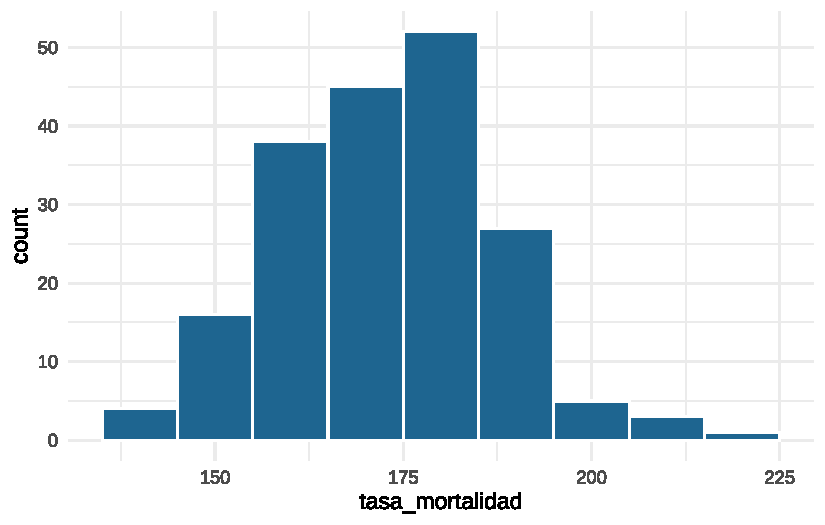
\includegraphics[width=0.85\linewidth,height=\textheight,keepaspectratio]{unidad_3/05_anova_files/figure-pdf/ej5-1.pdf}
\end{center}

\begin{Shaded}
\begin{Highlighting}[]
\CommentTok{\# boxplot}
\NormalTok{datos }\SpecialCharTok{|\textgreater{}}
  \FunctionTok{ggplot}\NormalTok{(}\AttributeTok{mapping =} \FunctionTok{aes}\NormalTok{(}\AttributeTok{y =}\NormalTok{ tasa\_mortalidad)) }\SpecialCharTok{+}
  \FunctionTok{geom\_boxplot}\NormalTok{(}\AttributeTok{fill =} \StringTok{"\#B2D680"}\NormalTok{) }\SpecialCharTok{+}
  \FunctionTok{theme\_minimal}\NormalTok{() }\CommentTok{\# tema claro}
\end{Highlighting}
\end{Shaded}

\begin{center}
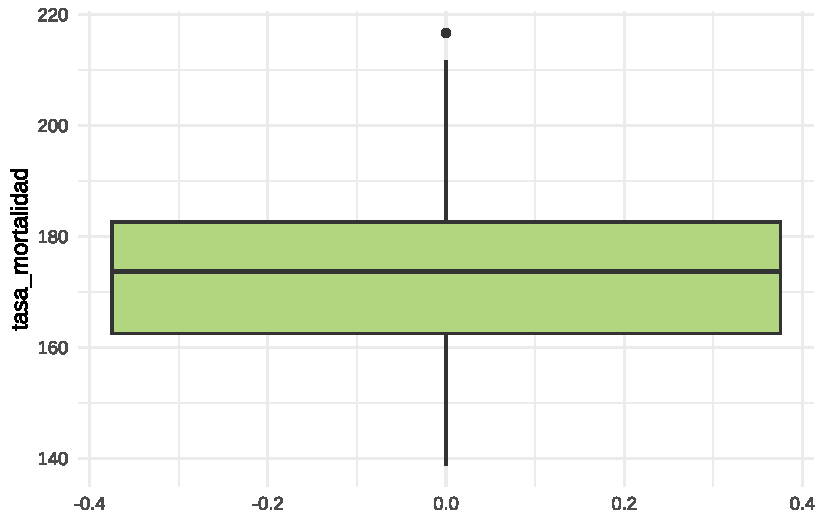
\includegraphics[width=0.85\linewidth,height=\textheight,keepaspectratio]{unidad_3/05_anova_files/figure-pdf/ej5-2.pdf}
\end{center}

La distribución global es simétrica pareciera existir un valor atípico.

Ahora veamos como es la distribución de la tasa de mortalidad por
estado.

\begin{Shaded}
\begin{Highlighting}[]
\CommentTok{\# Histograma por grupos}
\NormalTok{datos }\SpecialCharTok{|\textgreater{}}
  \FunctionTok{ggplot}\NormalTok{(}\AttributeTok{mapping =} \FunctionTok{aes}\NormalTok{(}\AttributeTok{x =}\NormalTok{ tasa\_mortalidad, }\AttributeTok{fill =}\NormalTok{ estado)) }\SpecialCharTok{+}
  \FunctionTok{geom\_histogram}\NormalTok{(}\AttributeTok{binwidth =} \DecValTok{10}\NormalTok{, }\AttributeTok{color =} \StringTok{"white"}\NormalTok{) }\SpecialCharTok{+}
  \FunctionTok{scale\_fill\_viridis\_d}\NormalTok{() }\SpecialCharTok{+} \CommentTok{\# paleta colorblind{-}friendly}
  \FunctionTok{facet\_grid}\NormalTok{(estado }\SpecialCharTok{\textasciitilde{}}\NormalTok{ .) }\SpecialCharTok{+} \CommentTok{\# variable estado en filas}
  \FunctionTok{theme\_minimal}\NormalTok{() }\CommentTok{\# tema claro}
\end{Highlighting}
\end{Shaded}

\begin{center}
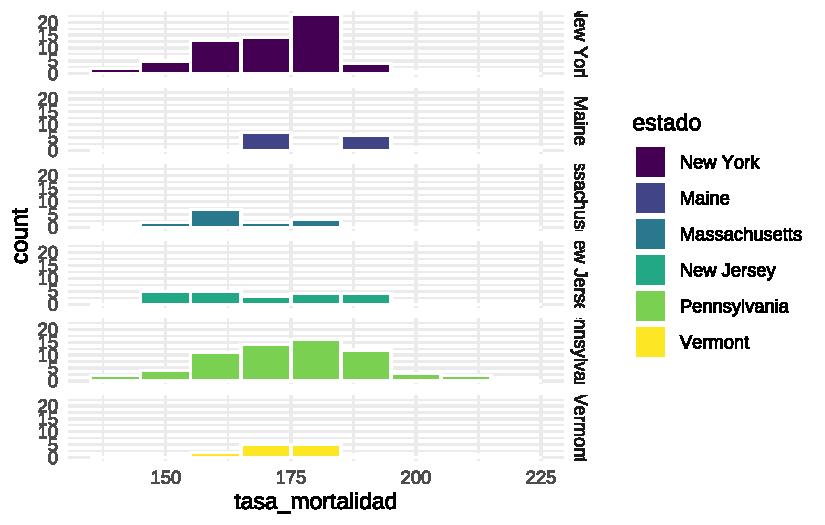
\includegraphics[width=0.85\linewidth,height=\textheight,keepaspectratio]{unidad_3/05_anova_files/figure-pdf/ej6-1.pdf}
\end{center}

\begin{Shaded}
\begin{Highlighting}[]
\CommentTok{\# Boxplot por grupos}
\NormalTok{datos }\SpecialCharTok{|\textgreater{}}
  \FunctionTok{ggplot}\NormalTok{(}\AttributeTok{mapping =} \FunctionTok{aes}\NormalTok{(}\AttributeTok{x =}\NormalTok{ estado, }\AttributeTok{y =}\NormalTok{ tasa\_mortalidad, }\AttributeTok{fill =}\NormalTok{ estado)) }\SpecialCharTok{+}
  \FunctionTok{geom\_boxplot}\NormalTok{() }\SpecialCharTok{+}
  \FunctionTok{scale\_fill\_viridis\_d}\NormalTok{() }\SpecialCharTok{+} \CommentTok{\# paleta colorblind{-}friendly}
  \FunctionTok{theme\_minimal}\NormalTok{() }\SpecialCharTok{+} \CommentTok{\# tema claro}
  \FunctionTok{theme}\NormalTok{(}\AttributeTok{axis.text.x =} \FunctionTok{element\_text}\NormalTok{(}\AttributeTok{angle =} \DecValTok{90}\NormalTok{)) }\CommentTok{\# gira etiquetas eje x}
\end{Highlighting}
\end{Shaded}

\begin{center}
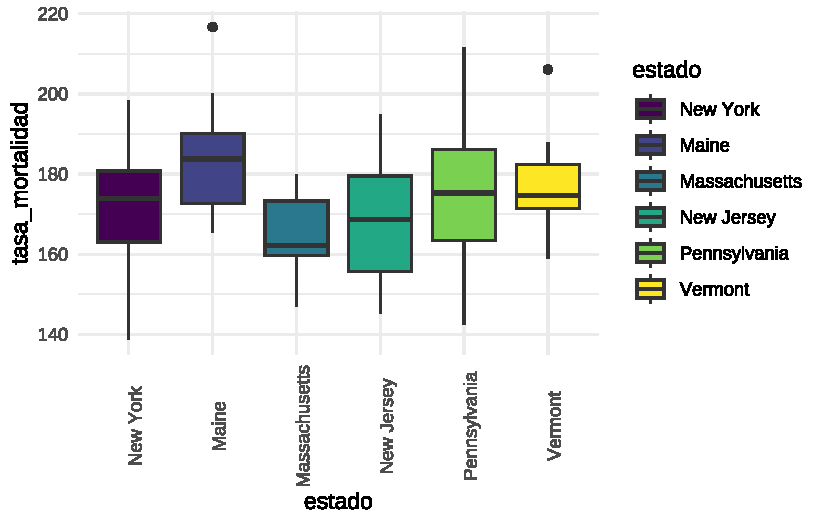
\includegraphics[width=0.85\linewidth,height=\textheight,keepaspectratio]{unidad_3/05_anova_files/figure-pdf/ej6-2.pdf}
\end{center}

Observamos que las distribuciones en algunos grupos parecen simétricas y
hay diferencias visuales entre las medianas. Esto plantea la pregunta de
si dichas diferencias son estadísticamente significativas.

\subsection{Análisis de supuestos}\label{anuxe1lisis-de-supuestos}

Si bien es más recomendable y habitual realizar el análisis de supuestos
a partir de los residuales del modelo, podemos chequear que la variable
dependiente cumpla con los supuestos de normalidad y homocedasticidad
previo a realizar el análisis.

\subsubsection{Normalidad}\label{normalidad-1}

Usamos el test de Kolmogorov-Smirnov con corrección de Lilliefors para
grupos con más de 50 observaciones con la función \texttt{lillie.test()}
del paquete \texttt{nortest}. Como algunos grupos tienen menos de 50
observaciones, también podríamos utilizar el test de Shapiro-Wilk
mediante la función \texttt{shapiro.test()} de R \texttt{base}:

\begin{Shaded}
\begin{Highlighting}[]
\NormalTok{datos }\SpecialCharTok{|\textgreater{}}
  \FunctionTok{filter}\NormalTok{(estado }\SpecialCharTok{==} \StringTok{"New York"}\NormalTok{) }\SpecialCharTok{|\textgreater{}}
  \FunctionTok{pull}\NormalTok{(tasa\_mortalidad) }\SpecialCharTok{|\textgreater{}} \CommentTok{\# con pull() extraemos datos de tasa\_mortalidad como vector}
  \FunctionTok{lillie.test}\NormalTok{() }\CommentTok{\# aplicamos test de bondad de ajuste}
\end{Highlighting}
\end{Shaded}

\begin{verbatim}

    Lilliefors (Kolmogorov-Smirnov) normality test

data:  pull(filter(datos, estado == "New York"), tasa_mortalidad)
D = 0.11633, p-value = 0.03637
\end{verbatim}

\begin{Shaded}
\begin{Highlighting}[]
\NormalTok{datos }\SpecialCharTok{|\textgreater{}}
  \FunctionTok{filter}\NormalTok{(estado }\SpecialCharTok{==} \StringTok{"Maine"}\NormalTok{) }\SpecialCharTok{|\textgreater{}}
  \FunctionTok{pull}\NormalTok{(tasa\_mortalidad) }\SpecialCharTok{|\textgreater{}} \CommentTok{\# con pull() extraemos datos de tasa\_mortalidad como vector}
  \FunctionTok{lillie.test}\NormalTok{() }\CommentTok{\# aplicamos test de bondad de ajuste}
\end{Highlighting}
\end{Shaded}

\begin{verbatim}

    Lilliefors (Kolmogorov-Smirnov) normality test

data:  pull(filter(datos, estado == "Maine"), tasa_mortalidad)
D = 0.18801, p-value = 0.1364
\end{verbatim}

\begin{Shaded}
\begin{Highlighting}[]
\NormalTok{datos }\SpecialCharTok{|\textgreater{}}
  \FunctionTok{filter}\NormalTok{(estado }\SpecialCharTok{==} \StringTok{"Massachusetts"}\NormalTok{) }\SpecialCharTok{|\textgreater{}}
  \FunctionTok{pull}\NormalTok{(tasa\_mortalidad) }\SpecialCharTok{|\textgreater{}} \CommentTok{\# con pull() extraemos datos de tasa\_mortalidad como vector}
  \FunctionTok{lillie.test}\NormalTok{() }\CommentTok{\# aplicamos test de bondad de ajuste}
\end{Highlighting}
\end{Shaded}

\begin{verbatim}

    Lilliefors (Kolmogorov-Smirnov) normality test

data:  pull(filter(datos, estado == "Massachusetts"), tasa_mortalidad)
D = 0.1591, p-value = 0.4377
\end{verbatim}

\begin{Shaded}
\begin{Highlighting}[]
\NormalTok{datos }\SpecialCharTok{|\textgreater{}}
  \FunctionTok{filter}\NormalTok{(estado }\SpecialCharTok{==} \StringTok{"New Jersey"}\NormalTok{) }\SpecialCharTok{|\textgreater{}}
  \FunctionTok{pull}\NormalTok{(tasa\_mortalidad) }\SpecialCharTok{|\textgreater{}} \CommentTok{\# con pull() extraemos datos de tasa\_mortalidad como vector}
  \FunctionTok{lillie.test}\NormalTok{() }\CommentTok{\# aplicamos test de bondad de ajuste}
\end{Highlighting}
\end{Shaded}

\begin{verbatim}

    Lilliefors (Kolmogorov-Smirnov) normality test

data:  pull(filter(datos, estado == "New Jersey"), tasa_mortalidad)
D = 0.14095, p-value = 0.3387
\end{verbatim}

\begin{Shaded}
\begin{Highlighting}[]
\NormalTok{datos }\SpecialCharTok{|\textgreater{}}
  \FunctionTok{filter}\NormalTok{(estado }\SpecialCharTok{==} \StringTok{"Pennsylvania"}\NormalTok{) }\SpecialCharTok{|\textgreater{}}
  \FunctionTok{pull}\NormalTok{(tasa\_mortalidad) }\SpecialCharTok{|\textgreater{}} \CommentTok{\# con pull() extraemos datos de tasa\_mortalidad como vector}
  \FunctionTok{lillie.test}\NormalTok{() }\CommentTok{\# aplicamos test de bondad de ajuste}
\end{Highlighting}
\end{Shaded}

\begin{verbatim}

    Lilliefors (Kolmogorov-Smirnov) normality test

data:  pull(filter(datos, estado == "Pennsylvania"), tasa_mortalidad)
D = 0.066685, p-value = 0.6839
\end{verbatim}

\begin{Shaded}
\begin{Highlighting}[]
\NormalTok{datos }\SpecialCharTok{|\textgreater{}}
  \FunctionTok{filter}\NormalTok{(estado }\SpecialCharTok{==} \StringTok{"Vermont"}\NormalTok{) }\SpecialCharTok{|\textgreater{}}
  \FunctionTok{pull}\NormalTok{(tasa\_mortalidad) }\SpecialCharTok{|\textgreater{}} \CommentTok{\# con pull() extraemos datos de tasa\_mortalidad como vector}
  \FunctionTok{lillie.test}\NormalTok{() }\CommentTok{\# aplicamos test de bondad de ajuste}
\end{Highlighting}
\end{Shaded}

\begin{verbatim}

    Lilliefors (Kolmogorov-Smirnov) normality test

data:  pull(filter(datos, estado == "Vermont"), tasa_mortalidad)
D = 0.14856, p-value = 0.5497
\end{verbatim}

Podemos graficar el comportamiento de la variable dependiente en cada
grupo mediante Q-Q plots usando el paquete \texttt{ggplot2}:

\begin{Shaded}
\begin{Highlighting}[]
\NormalTok{datos }\SpecialCharTok{|\textgreater{}}
  \FunctionTok{ggplot}\NormalTok{() }\SpecialCharTok{+}
  \FunctionTok{geom\_qq}\NormalTok{(}\AttributeTok{mapping =} \FunctionTok{aes}\NormalTok{(}\AttributeTok{sample =}\NormalTok{ tasa\_mortalidad)) }\SpecialCharTok{+}
  \FunctionTok{geom\_qq\_line}\NormalTok{(}\AttributeTok{mapping =} \FunctionTok{aes}\NormalTok{(}\AttributeTok{sample =}\NormalTok{ tasa\_mortalidad)) }\SpecialCharTok{+}
  \FunctionTok{facet\_wrap}\NormalTok{(}\SpecialCharTok{\textasciitilde{}}\NormalTok{estado) }\SpecialCharTok{+}
  \FunctionTok{theme\_minimal}\NormalTok{()}
\end{Highlighting}
\end{Shaded}

\begin{center}
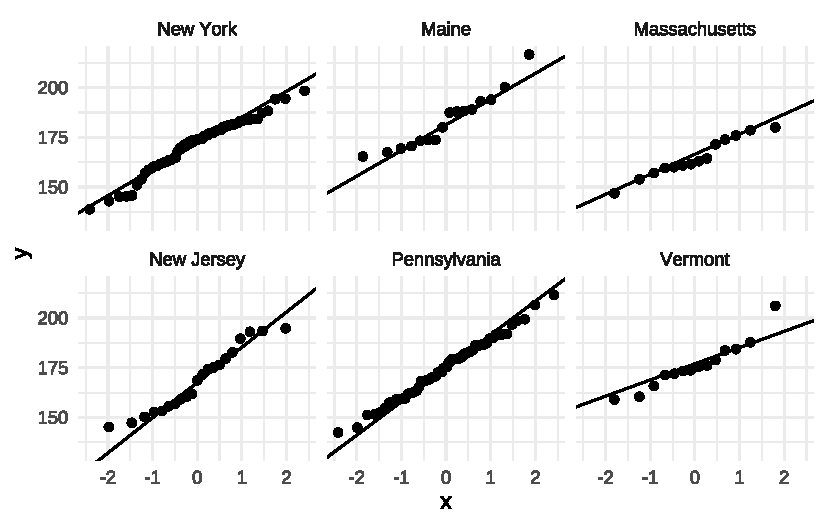
\includegraphics[width=0.85\linewidth,height=\textheight,keepaspectratio]{unidad_3/05_anova_files/figure-pdf/ej8-1.pdf}
\end{center}

\subsubsection{Homocedasticidad}\label{homocedasticidad-1}

Verificamos la homogeneidad de varianzas por grupo con el test de
Bartlett:

\begin{Shaded}
\begin{Highlighting}[]
\FunctionTok{bartlett.test}\NormalTok{(}
\NormalTok{  tasa\_mortalidad }\SpecialCharTok{\textasciitilde{}}\NormalTok{ estado, }\CommentTok{\# utiliza sintaxis fórmula}
  \AttributeTok{data =}\NormalTok{ datos}
\NormalTok{)}
\end{Highlighting}
\end{Shaded}

\begin{verbatim}

    Bartlett test of homogeneity of variances

data:  tasa_mortalidad by estado
Bartlett's K-squared = 4.8185, df = 5, p-value = 0.4384
\end{verbatim}

La variable respuesta cumple con el supuesto de homocedasticidad
(\(p = 0.438\)).

\subsection{Análisis de varianza}\label{anuxe1lisis-de-varianza}

Si bien podemos realizar un test ANOVA mediante la función
\texttt{aov()} de R \texttt{base}, en el contexto de este curso
utilizaremos la función \texttt{lm()} del paquete \texttt{stats} que
usamos anteriormente para ajustar el modelo de
\hyperref[regresiuxf3n-lineal-simple]{\textbf{regresión lineal
simple}}\textbf{:}

\begin{Shaded}
\begin{Highlighting}[]
\FunctionTok{lm}\NormalTok{(tasa\_mortalidad }\SpecialCharTok{\textasciitilde{}}\NormalTok{ estado, }\AttributeTok{data =}\NormalTok{ datos)}
\end{Highlighting}
\end{Shaded}

\begin{verbatim}

Call:
lm(formula = tasa_mortalidad ~ estado, data = datos)

Coefficients:
        (Intercept)          estadoMaine  estadoMassachusetts  
            171.640               11.510               -6.840  
   estadoNew Jersey   estadoPennsylvania        estadoVermont  
             -3.007                3.419                4.631  
\end{verbatim}

Siempre que trabajemos con modelos, conviene que asignemos los
resultados a objetos que luego nos servirán para aplicar otras
funciones. Como nuestra variable explicativa es categórica y nuestro
principal interés es conocer si existen diferencias significativas entre
grupos, no analizaremos los coeficientes del modelo con
\texttt{summary()}, sino la significancia del test F mediante la función
\texttt{anova()}.

\begin{Shaded}
\begin{Highlighting}[]
\CommentTok{\# ANOVA}
\NormalTok{modelo }\OtherTok{\textless{}{-}} \FunctionTok{lm}\NormalTok{(tasa\_mortalidad }\SpecialCharTok{\textasciitilde{}}\NormalTok{ estado, }\AttributeTok{data =}\NormalTok{ datos)}

\CommentTok{\# Salida del modelo}
\FunctionTok{anova}\NormalTok{(modelo)}
\end{Highlighting}
\end{Shaded}

\begin{verbatim}
Analysis of Variance Table

Response: tasa_mortalidad
           Df Sum Sq Mean Sq F value   Pr(>F)   
estado      5   3513  702.67  3.7103 0.003179 **
Residuals 185  35036  189.38                    
---
Signif. codes:  0 '***' 0.001 '**' 0.01 '*' 0.05 '.' 0.1 ' ' 1
\end{verbatim}

Los resultados del test F nos muestran un \(p = 0,003\), sugiriendo que
al menos dos grupos son diferentes entre sí.

\subsection{Comparaciones múltiples}\label{comparaciones-muxfaltiples}

Una vez que comprobamos que existen diferencias significativas entre
grupos, nos interesa saber cuáles grupos son diferentes entre sí. Para
ello, existen distintos algoritmos de comparaciones múltiples con sus
respectivas correcciones, como el test de \emph{Diferencia Honestamente
Significativa de Tukey,} también llamado Tukey HSD o \textbf{test de
Tukey}. Esta prueba se aplica para grupos equilibrados (mismo tamaño) y
varianzas similares (homocedásticas). Es una prueba conservadora, dado
que mantiene bajo el error de tipo I, sacrificando la capacidad de
detectar diferencias existentes.

Si las varianzas son homocedásticas pero los grupos difieren en tamaño,
podemos usar el test de Tukey si tenemos que comparar entre varios
grupos, o la \textbf{corrección de Bonferroni} para grupos más
reducidos.

{\def\LTcaptype{none} % do not increment counter
\begin{longtable}[]{@{}ll@{}}
\toprule\noalign{}
Código & Rango \\
\midrule\noalign{}
\endhead
\bottomrule\noalign{}
\endlastfoot
*** & 0 a 0,001 \\
** & 0,001 a 0,01 \\
* & 0,01 a 0,05 \\
. & 0,05 a 0,1 \\
& 0,1 a 1 \\
\end{longtable}
}

El paquete \texttt{emmeans} (Lenth y Piaskowski 2026) es una herramienta
muy versátil y poderosa para realizar comparaciones múltiples.
Comenzaremos utilizando la función \texttt{emmeans()} con el argumento
\texttt{specs\ =\ "estado"} para crear un objeto que contenga las medias
marginales por grupo:

\begin{Shaded}
\begin{Highlighting}[]
\NormalTok{comp }\OtherTok{\textless{}{-}} \FunctionTok{emmeans}\NormalTok{(modelo, }\AttributeTok{specs =} \StringTok{"estado"}\NormalTok{)}
\end{Highlighting}
\end{Shaded}

Para realizar las comparaciones múltiples mediante test de Tukey usamos
el comando \texttt{contrast()} con el argumento
\texttt{method\ =\ "pairwise"}:

\begin{Shaded}
\begin{Highlighting}[]
\FunctionTok{contrast}\NormalTok{(comp, }\AttributeTok{method =} \StringTok{"pairwise"}\NormalTok{)}
\end{Highlighting}
\end{Shaded}

\begin{verbatim}
 contrast                     estimate   SE  df t.ratio p.value
 New York - Maine               -11.51 3.86 185  -2.983  0.0376
 New York - Massachusetts         6.84 4.07 185   1.680  0.5469
 New York - New Jersey            3.01 3.47 185   0.865  0.9542
 New York - Pennsylvania         -3.42 2.45 185  -1.394  0.7305
 New York - Vermont              -4.63 4.07 185  -1.137  0.8652
 Maine - Massachusetts           18.35 5.04 185   3.644  0.0046
 Maine - New Jersey              14.52 4.57 185   3.179  0.0211
 Maine - Pennsylvania             8.09 3.85 185   2.103  0.2901
 Maine - Vermont                  6.88 5.04 185   1.366  0.7474
 Massachusetts - New Jersey      -3.83 4.75 185  -0.807  0.9659
 Massachusetts - Pennsylvania   -10.26 4.06 185  -2.527  0.1217
 Massachusetts - Vermont        -11.47 5.20 185  -2.205  0.2402
 New Jersey - Pennsylvania       -6.43 3.46 185  -1.857  0.4322
 New Jersey - Vermont            -7.64 4.75 185  -1.609  0.5939
 Pennsylvania - Vermont          -1.21 4.06 185  -0.299  0.9997

P value adjustment: tukey method for comparing a family of 6 estimates 
\end{verbatim}

Los resultados del test de Tukey nos muestran diferencias significativas
en la tasa de mortalidad por cáncer en el estado de Maine respecto de
New York, Massachusetts y New Jersey.

Para mayor claridad, podemos mostrar las comparaciones múltiples
mediante un gráfico:

\begin{Shaded}
\begin{Highlighting}[]
\FunctionTok{plot}\NormalTok{(comp) }\SpecialCharTok{+}
  \FunctionTok{theme\_minimal}\NormalTok{() }\CommentTok{\# tema claro}
\end{Highlighting}
\end{Shaded}

\begin{center}
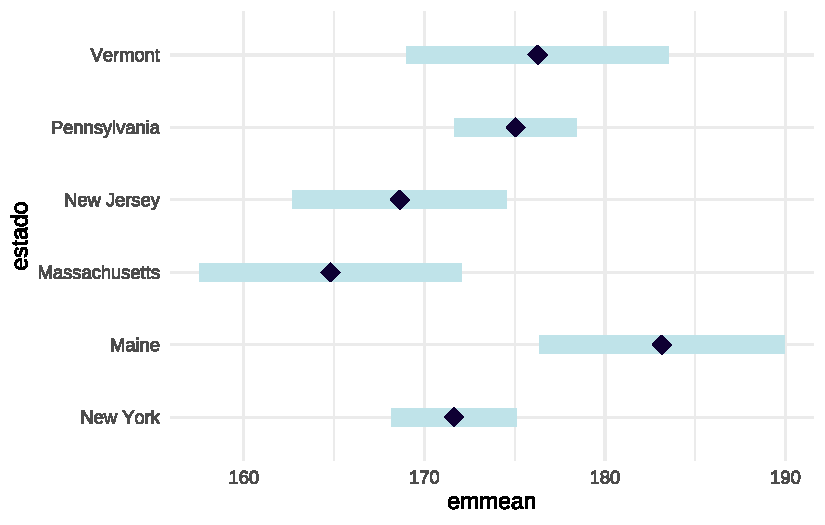
\includegraphics[width=0.85\linewidth,height=\textheight,keepaspectratio]{unidad_3/05_anova_files/figure-pdf/ej14-1.pdf}
\end{center}

El rombo del medio representa la media marginal para cada grupo y el
rectángulo azul, su intervalo de confianza, aquellos grupos en los que
no se superponen los intervalos de confianza son estadísticamente
diferentes entre sí.

\subsection{Bondad de ajuste}\label{bondad-de-ajuste}

El tamaño de efecto comúnmente utilizado para el caso de ANOVA es
\(\eta^2\) (\emph{eta-cuadrado)}, que se calcula como el cociente de la
suma de cuadrados del efecto sobre la suma de cuadrados total.

\begin{Shaded}
\begin{Highlighting}[]
\FunctionTok{anova}\NormalTok{(modelo)}
\end{Highlighting}
\end{Shaded}

\begin{verbatim}
Analysis of Variance Table

Response: tasa_mortalidad
           Df Sum Sq Mean Sq F value   Pr(>F)   
estado      5   3513  702.67  3.7103 0.003179 **
Residuals 185  35036  189.38                    
---
Signif. codes:  0 '***' 0.001 '**' 0.01 '*' 0.05 '.' 0.1 ' ' 1
\end{verbatim}

\begin{Shaded}
\begin{Highlighting}[]
\CommentTok{\# calculo eta{-}cuadrado}
\NormalTok{eta2 }\OtherTok{\textless{}{-}} \DecValTok{3513} \SpecialCharTok{/}\NormalTok{ (}\DecValTok{3513} \SpecialCharTok{+} \DecValTok{35036}\NormalTok{)}

\NormalTok{eta2}
\end{Highlighting}
\end{Shaded}

\begin{verbatim}
[1] 0.09113077
\end{verbatim}

Podemos llegar al mismo valor usando la función \texttt{r2()} del
paquete \texttt{performance}:

\begin{Shaded}
\begin{Highlighting}[]
\FunctionTok{r2}\NormalTok{(modelo)}
\end{Highlighting}
\end{Shaded}

\begin{verbatim}
# R2 for Linear Regression
       R2: 0.091
  adj. R2: 0.067
\end{verbatim}

\subsection{Potencia}\label{potencia}

Los test de potencia permiten determinar la probabilidad de encontrar
diferencias significativas entre las medias para un determinado nivel de
significancia indicando el tamaño de los grupos.

En base al eta-cuadrado obtenido anteriormente, calculamos el tamaño de
efecto convencional mediante la función \texttt{cohen.ES()} del paquete
\texttt{pwr} (Champely 2020):

\begin{Shaded}
\begin{Highlighting}[]
\FunctionTok{cohen.ES}\NormalTok{(}\AttributeTok{test =} \StringTok{"anov"}\NormalTok{, }\AttributeTok{size =} \StringTok{"small"}\NormalTok{)}
\end{Highlighting}
\end{Shaded}

\begin{verbatim}

     Conventional effect size from Cohen (1982) 

           test = anov
           size = small
    effect.size = 0.1
\end{verbatim}

La función \texttt{pwr.anova.test()} del paquete \texttt{pwr} nos
permite calcular la potencia en base al número de grupos, número de
observaciones por grupo, tamaño de efecto y nivel de significancia
(habitualmente 0,05).

Para grupos de igual tamaño usamos el siguiente código:

\begin{Shaded}
\begin{Highlighting}[]
\FunctionTok{pwr.anova.test}\NormalTok{(}\AttributeTok{k =}\NormalTok{ k, }\AttributeTok{n =}\NormalTok{ n, }\AttributeTok{f =}\NormalTok{ eta\_cuadrado, }\AttributeTok{sig.level =} \FloatTok{0.05}\NormalTok{)}
\end{Highlighting}
\end{Shaded}

En nuestro ejemplo, donde los tamaños de grupo son diferentes, primero
debemos calcular el tamaño de grupo efectivo:

\begin{Shaded}
\begin{Highlighting}[]
\CommentTok{\# Número de grupos}
\NormalTok{k }\OtherTok{\textless{}{-}} \FunctionTok{nlevels}\NormalTok{(datos}\SpecialCharTok{$}\NormalTok{estado)}

\CommentTok{\# Número de observaciones por grupo}
\NormalTok{n }\OtherTok{\textless{}{-}} \FunctionTok{tabyl}\NormalTok{(datos}\SpecialCharTok{$}\NormalTok{estado)}\SpecialCharTok{$}\NormalTok{n}

\CommentTok{\# Tamaño de grupo efectivo}
\NormalTok{neff }\OtherTok{\textless{}{-}} \FunctionTok{sum}\NormalTok{(n)}\SpecialCharTok{\^{}}\DecValTok{2} \SpecialCharTok{/} \FunctionTok{sum}\NormalTok{(n}\SpecialCharTok{\^{}}\DecValTok{2}\NormalTok{)}
\end{Highlighting}
\end{Shaded}

Calculamos la potencia:

\begin{Shaded}
\begin{Highlighting}[]
\FunctionTok{pwr.anova.test}\NormalTok{(}\AttributeTok{k =}\NormalTok{ k, }\AttributeTok{n =}\NormalTok{ neff, }\AttributeTok{f =}\NormalTok{ eta2, }\AttributeTok{sig.level =} \FloatTok{0.05}\NormalTok{)}
\end{Highlighting}
\end{Shaded}

\begin{verbatim}

     Balanced one-way analysis of variance power calculation 

              k = 6
              n = 4.040425
              f = 0.09113077
      sig.level = 0.05
          power = 0.05670154

NOTE: n is number in each group
\end{verbatim}

\subsection{Análisis de residuales}\label{anuxe1lisis-de-residuales}

Para poder dar por válidos los resultados del ANOVA es necesario
verificar que se satisfacen las condiciones analizando los residuos del
modelo. Para ello, usaremos el mismo procedimiento que vimos para la
\hyperref[regresiuxf3n-lineal-simple]{\textbf{regresión lineal simple}}.

Método gráfico con paquete \texttt{performance}:

\begin{Shaded}
\begin{Highlighting}[]
\FunctionTok{check\_model}\NormalTok{(modelo)}
\end{Highlighting}
\end{Shaded}

\begin{center}
\includegraphics[width=0.85\linewidth,height=\textheight,keepaspectratio]{unidad_3/05_anova_files/figure-pdf/ej21-1.pdf}
\end{center}

Chequeo normalidad de residuales mediante test de Lilliefors:

\begin{Shaded}
\begin{Highlighting}[]
\FunctionTok{lillie.test}\NormalTok{(modelo}\SpecialCharTok{$}\NormalTok{residuals)}
\end{Highlighting}
\end{Shaded}

\begin{verbatim}

    Lilliefors (Kolmogorov-Smirnov) normality test

data:  modelo$residuals
D = 0.046833, p-value = 0.388
\end{verbatim}

Chequeo homocedasticidad (test de Breusch-Pagan):

\begin{Shaded}
\begin{Highlighting}[]
\FunctionTok{check\_heteroscedasticity}\NormalTok{(modelo)}
\end{Highlighting}
\end{Shaded}

\begin{verbatim}
OK: Error variance appears to be homoscedastic (p = 0.597).
\end{verbatim}

Chequeo presencia de outliers (distancia de Cook):

\begin{Shaded}
\begin{Highlighting}[]
\FunctionTok{check\_outliers}\NormalTok{(modelo)}
\end{Highlighting}
\end{Shaded}

\begin{verbatim}
OK: No outliers detected.
- Based on the following method and threshold: cook (0.5).
- For variable: (Whole model)
\end{verbatim}

\section{Conclusión}\label{conclusiuxf3n}

Se ha realizado un ANOVA de una vía para comparar la tasa de mortalidad
por cáncer en seis estados de Estados Unidos. Se encontraron diferencias
estadísticamente significativas entre las medias de los grupos (F =
3,71, p = 0.003). El \emph{eta-cuadrado} fue de 0.091, lo que indica que
el estado de residencia explica un 9.1\% de la varianza total en los
valores de la tasa de mortalidad por cáncer. La potencia de la prueba
estadística fue del 5.7\%.

Se realizó la prueba post hoc de Tukey HSD y se encontró que media de
mortalidad para el estado de Maine fue estadísticamente superiror
respecto de los estados de Massachusetts, New York y New Jersey (p
\textless{} 0.05).

Agresti (2015)

Triola (2018)

Sjoberg et~al. (2021)

Lüdecke et~al. (2022)

Gross y Ligges (2015)

Ryu (2025)

Waring et~al. (2026)

\section*{Referencias}\label{referencias-15}
\addcontentsline{toc}{section}{Referencias}

\markright{Referencias}

\chapter{Rol de las variables}\label{rol-de-las-variables}

\section{Introducción}\label{introducciuxf3n-15}

Antes de comenzar a construir modelos de
\href{07_reg_lineal_multiple.qmd}{\textbf{regresión lineal múltiple}},
es necesario repasar algunos conceptos fundamentales.

Los estudios epidemiológicos suelen partir de modelos teóricos
conocidos, consensos científicos establecidos o hipotéticos, intentando
responder a una pregunta de investigación. Las variables recolectadas se
definen en la etapa de diseño del estudio, cada una cumpliendo un rol
específico producto del modelo teórico asumido que dialoga con el estado
del arte del tema investigado.Como mínimo, se identifican dos variables
principales y excluyentes: la exposición (variable independiente) y el
desenlace (variable dependiente). Una vez seleccionadas la variable
dependiente e independiente, las demás variables medidas o no medidas
son las que se denominan covariables.

En el marco de nuestros estudios, las covariables pueden asumir diversos
roles, como confusoras, intermedias, colisionadoras, modificadoras de
efecto, entre otros. Algunos de estos roles suelen estar definidos
previamente por la literatura mientras que otros pueden surgir como
hipotéticas o ser identificados durante el análisis.

Por ello, la/el epidemióloga/o debe definir un marco teórico previo y
conocer qué alcance tiene el tipo de estudio desarrollado.

\section{Causalidad vs asociación}\label{causalidad-vs-asociaciuxf3n}

Un error persistente en la práctica es suponer que los modelos de
regresión (lineales, logísticos, etc) poseen la capacidad intrínseca de
discernir causalidad. Sin embargo, estos modelos son
\emph{``agnósticos''}: procesan datos y devuelven coeficientes basados
exclusivamente en correlaciones matemáticas, sin comprender la
naturaleza biológica o social de las variables. Por ello, el
epidemiólogo debe definir un marco teórico previo y conocer que alcance
tiene el tipo de estudio desarrollado.

Partiendo de la premisa que asociación no implica causalidad, podemos
razonar causalmente para decidir qué variables controlar o que ajustes
hacer en el análisis, aun cuando al final concluyamos que los datos no
permiten establecer causalidad con certeza. De hecho, si no razonamos
causalmente sobre el rol de las variables, no podemos saber si la
estimación obtenida del modelo como mera asociación es siquiera válida
internamente.

Los estudios observacionales trabajan muchas veces con asociaciones y
para aproximarnos a responder las preguntas de investigación que nos
hacemos es necesario tener presente algunas cuestiones: criterios de
causalidad (temporalidad, plausibilidad biológica, socioeconómica, etc),
presencia de variables de confusión, sesgos y estructura causal
subyacente.

Para formalizar estos razonamientos, se suelen utilizar los \emph{Grafos
Acíclicos Dirigidos} (DAG, por sus siglas en inglés), herramientas que
permiten visualizar supuestos y detectar sesgos estructurales antes de
avanzar con la metodología.

\section{El rol de las variables}\label{el-rol-de-las-variables}

Los roles de confusora, mediadora, colisionadora o modificadora del
efecto son propiedades que emergen de la estructura causal del fenómeno
que se estudia (representada en el DAG) y no del diseño del estudio. El
tabaquismo es un factor de riesgo con efecto causal sobre el cáncer, la
edad es causa de tabaquismo y cáncer, la hospitalización es consecuencia
de ambos: eso es cierto independientemente de si llegamos a esos datos a
un diseño de cohorte, casos-controles o estudio transversal.

Lo que cambia según el diseño no es la estructura causal subyacente,
sino dos cosas:

\begin{itemize}
\tightlist
\item
  Lo que podemos estimar (un OR en lugar de RR, prevalencia en lugar de
  incidencia, etc.)
\item
  Los riesgos estructurales de sesgo que introduce el propio diseño
\end{itemize}

\section{Los DAGs}\label{los-dags}

Un \emph{Grafo Acíclico Dirigido} (\textbf{DAG}) es un grafo donde los
nodos representan variables y las flechas representan efectos causales
directos. \emph{``Acíclico''} significa que no hay ciclos: ninguna
variable puede causarse a sí misma a través de una cadena de efectos.

\subsection{Convenciones básicas}\label{convenciones-buxe1sicas}

\begin{itemize}
\tightlist
\item
  \(X \rightarrow Y\) se lee: \emph{X tiene un efecto causal directo
  sobre Y}
\item
  La ausencia de flechas entre dos variables significa que no existe
  efecto causal directo entre ellas (no implica que la asociación
  estadística sea cero)
\item
  Los DAG son cualitativos, representan la presencia o ausencia de
  efectos, no su magnitud.
\end{itemize}

\subsection{Caminos en un DAG}\label{caminos-en-un-dag}

Un camino entre dos nodos es cualquier secuencia de flechas que los
conecta, independientemente de la dirección. Existen tres tipos de
estructuras básicas:

{\def\LTcaptype{none} % do not increment counter
\begin{longtable}[]{@{}ll@{}}
\toprule\noalign{}
Estructura del DAG & Nombre \\
\midrule\noalign{}
\endhead
\bottomrule\noalign{}
\endlastfoot
X --\textgreater{} M --\textgreater{} Y & Cadena (mediación) \\
X \textless-- Z --\textgreater{} Y & Bifurcación (confusión) \\
X --\textgreater{} C \textless-- Y & Colisionador \\
\end{longtable}
}

Usamos los DAG, a \emph{priori}, como una representación gráfica de las
suposiciones causales que como investigadores tenemos antes de analizar
los datos. Nos permite visualizar qué variables debemos ajustar
(controlar confusión) y cuales no debemos incluir para evitar sesgos,
independientemente del diseño de estudio. Además, nos obliga a
explicitar el modelo teórico subyacente y a formular hipótesis causales
plausibles.

\section{Confusión}\label{confusiuxf3n}

Una variable de confusión es una variable que distorsiona la medida de
asociación entre las variables principales del estudio
(exposición-desenlace). En presencia de confusión, pueden observarse los
siguientes escenarios:

\begin{itemize}
\item
  \textbf{Asociación espuria:} Efecto observado donde en realidad no
  existe.
\item
  \textbf{Confusión positiva:} Exageración o atenuación de una
  asociación real.
\item
  \textbf{Confusión negativa:} Inversión del sentido de una asociación
  real.
\end{itemize}

Según Gordis (2017), en un estudio que evalúa si la exposición (\(X\))
causa un resultado (\(Y\)), se dice que un tercer factor (\(Z\)) es una
variable de confusión si cumple con los siguientes criterios:

\begin{itemize}
\tightlist
\item
  \(Z\) es una causa (o proxy de una causa) conocido para \(Y\).
\item
  \(Z\) está asociado con la exposición \(X\), pero no es un resultado
  de \(X\).
\item
  \(Z\) no está en el camino causal entre \(X\) e \(Y\) (no es
  mediadora)
\end{itemize}

\protect\phantomsection\label{fig1}
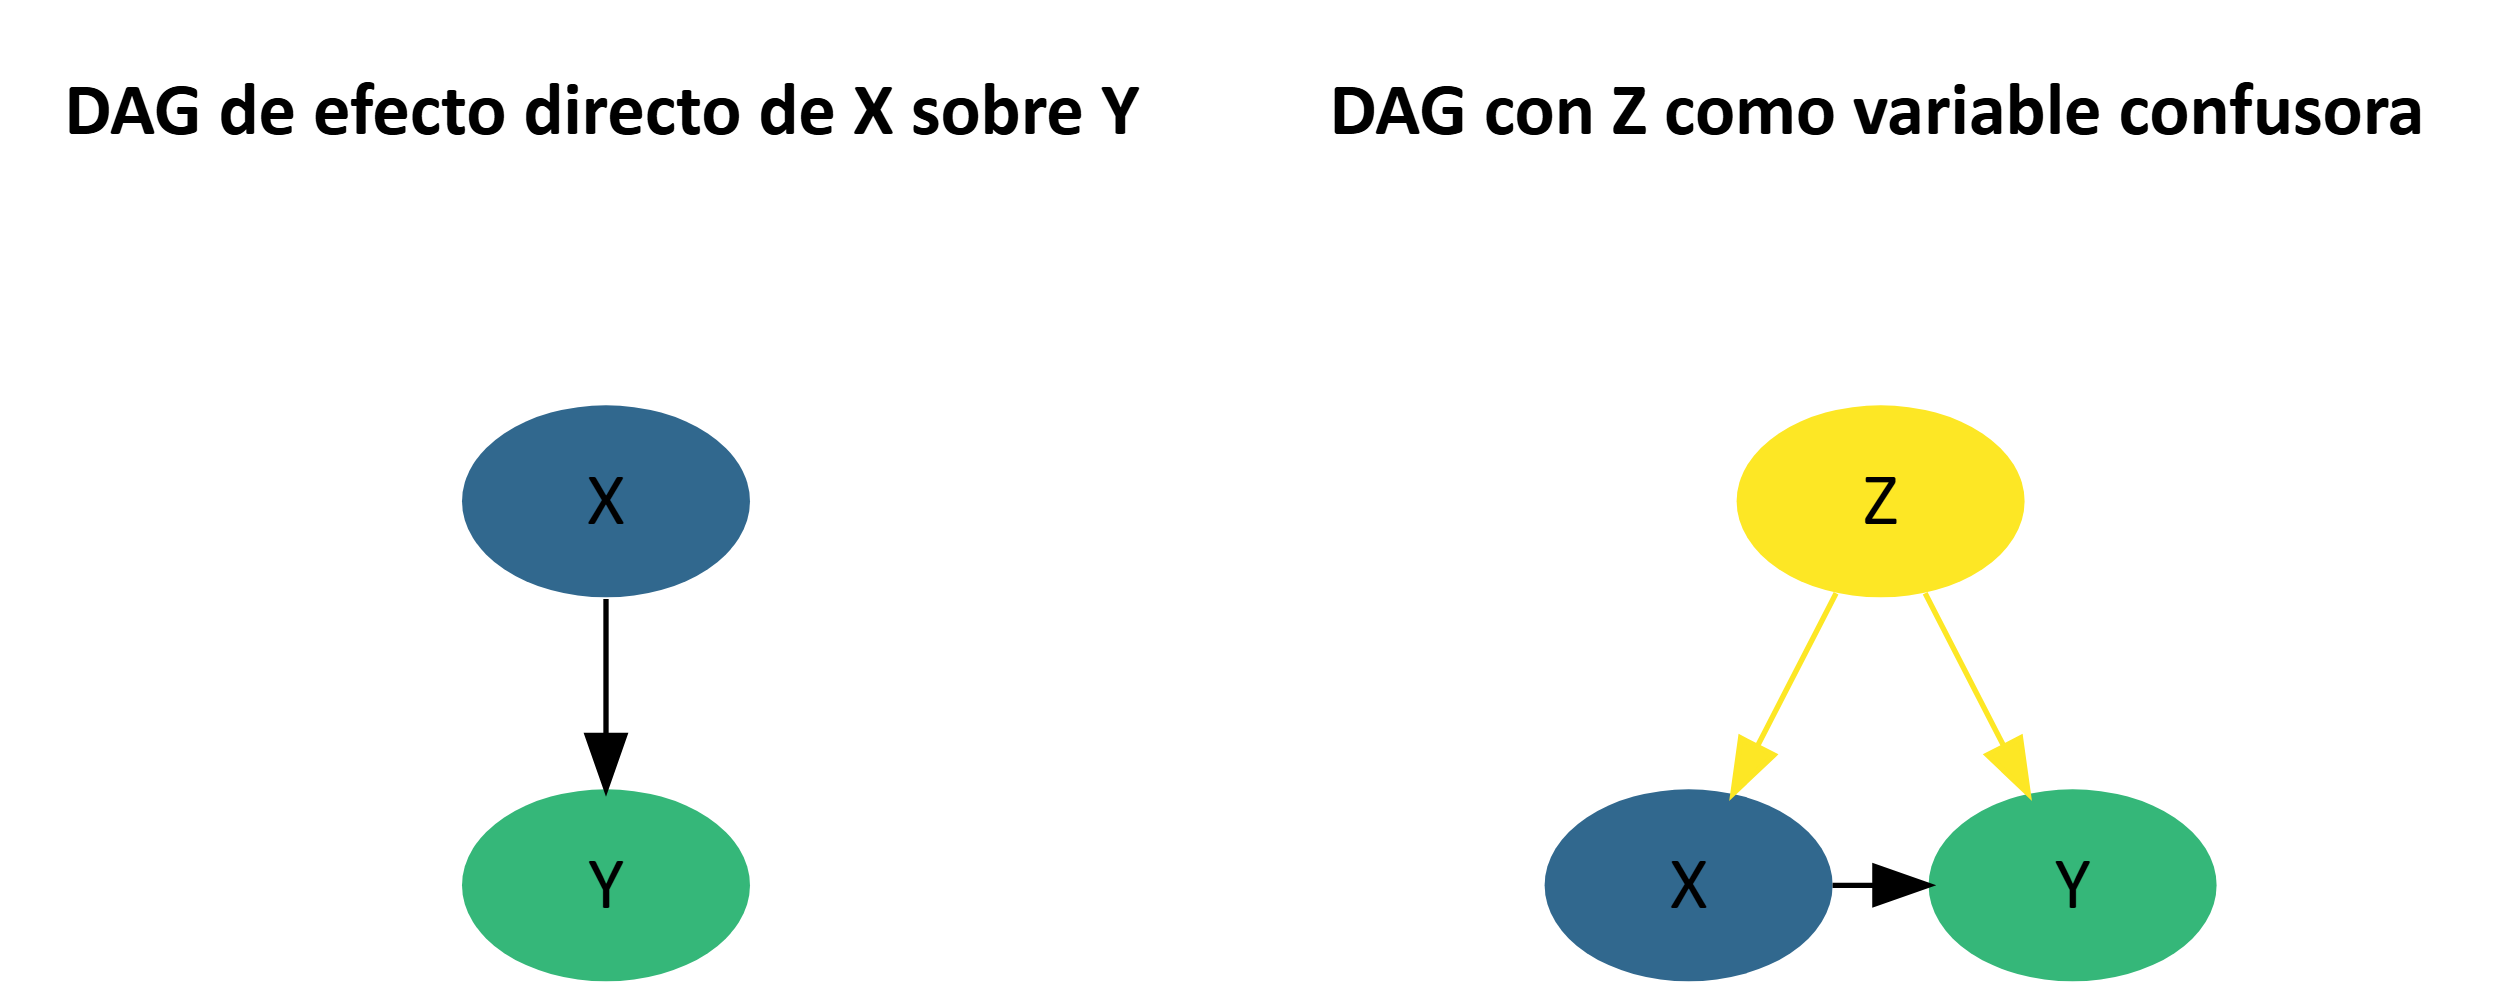
\includegraphics[width=5.5in,height=3.5in]{unidad_3/06_rol_variables_files/figure-latex/dot-figure-4.png}

Para quienes necesiten profundizar, se recomienda leer el artículo:

➡️ De Irala, J., et al.~(2001). ¿Qué es una variable de confusión?
\emph{Medicina Clínica}, \emph{117}(10), 377--385.
\url{https://doi.org/10.1016/S0025-7753(01)72121-5}

\subsection{Manejo de la confusión}\label{manejo-de-la-confusiuxf3n}

Dentro de las estrategias para manejar la confusión, podemos pensar en
dos momentos:

\begin{itemize}
\tightlist
\item
  A la hora de diseñar y llevar a cabo el estudio:

  \begin{itemize}
  \tightlist
  \item
    Emparejamiento individual.
  \item
    Emparejamiento de grupo.
  \end{itemize}
\item
  Al momento de analizar los datos:

  \begin{itemize}
  \tightlist
  \item
    Estratificación.
  \item
    Ajuste estadístico.
  \end{itemize}
\end{itemize}

El ajuste estadístico, característico de los análisis multivariados,
permite estimar el efecto específico de cada variable independiente
sobre la dependiente, controlando por las demás variables.

Un criterio estadístico comúnmente aceptado es que un factor se
considera confusor si el ajuste por dicha variable provoca un cambio de
al menos el 10\% en la magnitud de la asociación. Por ejemplo, edad y
sexo son variables frecuentemente confusoras en estudios epidemiológicos
y generalmente son pocos los trabajos que no presentan datos ajustados
por estas covariables.

En este curso utilizaremos la
\href{07_reg_lineal_multiple.qmd}{\textbf{regresión lineal múltiple}} y
los modelos lineales generalizados para manejar la confusión, ajustando
por múltiples covariables. A continuación, se ejemplifica el fenómeno
gráficamente con un diagrama de dispersión.

\begin{center}
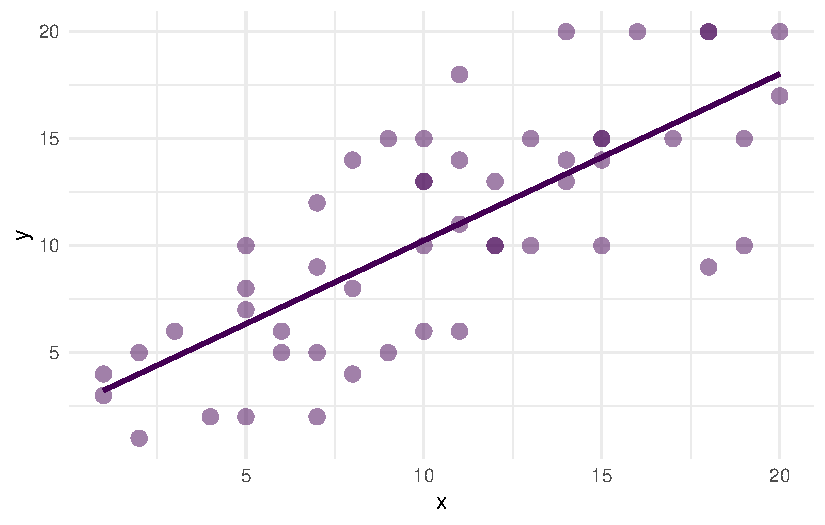
\includegraphics[width=0.85\linewidth,height=\textheight,keepaspectratio]{unidad_3/06_rol_variables_files/figure-pdf/fig2-1.pdf}
\end{center}

La recta de regresión muestra una correlación positiva entre los valores
de las variables, \(X\) e \(Y\), con una ecuación de la forma:

\[
\hat{y} = \beta_0 + \beta_1x_1 + \epsilon
\]

La salida en R de este modelo se vería de la siguiente forma:

\begin{verbatim}

Call:
lm(formula = y ~ x, data = datos_conf)

Residuals:
    Min      1Q  Median      3Q     Max 
-7.4701 -2.4124 -0.0179  2.5926  6.9821 

Coefficients:
            Estimate Std. Error t value Pr(>|t|)    
(Intercept)  2.45017    1.13262   2.163   0.0354 *  
x            0.77889    0.09642   8.078 1.45e-10 ***
---
Signif. codes:  0 '***' 0.001 '**' 0.01 '*' 0.05 '.' 0.1 ' ' 1

Residual standard error: 3.559 on 49 degrees of freedom
Multiple R-squared:  0.5712,    Adjusted R-squared:  0.5624 
F-statistic: 65.26 on 1 and 49 DF,  p-value: 1.45e-10
\end{verbatim}

El intercepto (\(\beta_0\)) es 2,45 y la pendiente (\(\beta_1\)) es
0,78. El modelo explica el 56\% de la variabilidad de \(Y\) (\(R^2\) =
0,56). En la ecuación podemos representarlo como:

\[
\hat{y} = 2.45 + 0.78x_1 + \epsilon
\]

Ahora incorporemos la covariable \(Z\), con categorías \textbf{A} y
\textbf{B}, que sospechamos tiene un rol de confusión en el modelo
teórico (DAG).

\begin{center}
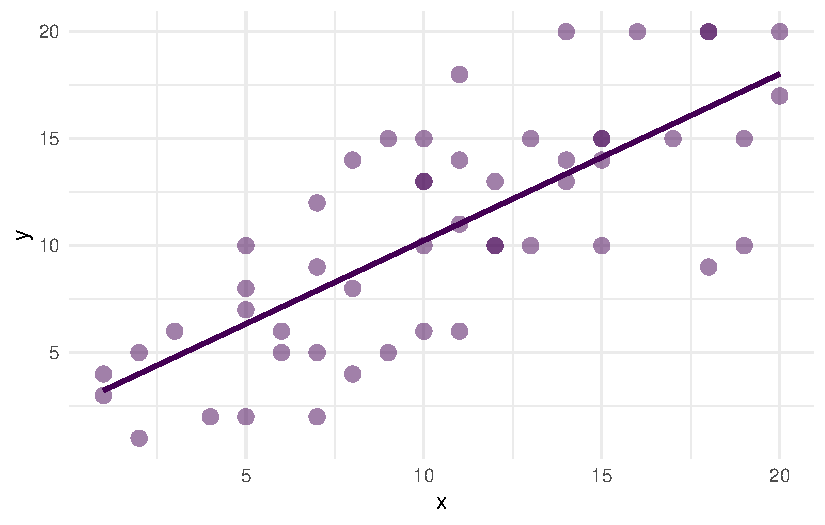
\includegraphics[width=0.85\linewidth,height=\textheight,keepaspectratio]{unidad_3/06_rol_variables_files/figure-pdf/fig3-1.pdf}
\end{center}

El gráfico de dispersión muestra que hay una diferencia entre las rectas
de regresión que se mantiene prácticamente constante (paralelas) en todo
su desarrollo. Esa distancia medida en valores de \(Y\) es \(\beta_2\):

\[
\hat{y} = \beta_0 + \beta_1x_1 + \beta_2x_2 + \epsilon
\]

Visto en resultados de consola:

\begin{verbatim}

Call:
lm(formula = y ~ x + z, data = datos_conf)

Residuals:
   Min     1Q Median     3Q    Max 
-7.958 -1.502 -0.225  1.840  5.652 

Coefficients:
            Estimate Std. Error t value Pr(>|t|)    
(Intercept)  0.65684    1.00484   0.654    0.516    
x            0.65260    0.08372   7.795 4.49e-10 ***
zB           4.55436    0.93258   4.884 1.20e-05 ***
---
Signif. codes:  0 '***' 0.001 '**' 0.01 '*' 0.05 '.' 0.1 ' ' 1

Residual standard error: 2.939 on 48 degrees of freedom
Multiple R-squared:  0.7135,    Adjusted R-squared:  0.7016 
F-statistic: 59.77 on 2 and 48 DF,  p-value: 9.347e-14
\end{verbatim}

El coeficiente \(\beta_1\) de la variable independiente principal
(\(X\)) varió al incorporar la nueva variable (\(Z\)), pasando de 0,78
(cruda) a 0,65 (ajustada), es decir que disminuyó casi un 20\%. A la
vez, la covariable tiene una relación significativa con la variable
dependiente (\(Y\)) y el modelo aumenta el \(R^2\) ajustado a 0,70.

Entonces podemos ver que la regresión multiple ajustó el efecto de \(X\)
sobre \(Y\), teniendo en cuenta el efecto confusor de \(Z\) que
sospechabamos. El valor de \(Y\) ahora es 0,66 (\(\beta_0\)) + 0,65* el
valor de \texttt{x} (\(\beta_1*x\)) mientras \(Z\) es igual al nivel de
referencia \textbf{A}, en cambio \(Y\) vale 0,66 (\(\beta_0\)) + 0,65*
el valor de \(X\) (\(\beta_1*x\)) + 4,55 (\(\beta_2\)) cuando \(Z\) es
igual a \textbf{B}.

\textbf{Nota}: No toda variable asociada con \(X\) e \(Y\) es confusora.
La estructura causal es la que define ese rol, que luego la matemática
del modelo confirmará. Una variable puede ser un proxy de la confusora
(que en la práctica es como tener a la variable confusora) o jugar otro
rol, siempre dependiendo de la pregunta de investigación que nos
hagamos.

\section{Variable mediadora}\label{variable-mediadora}

Una variable \(M\) es mediadora si se encuentra en la cadena causal
entre \(X\) e \(Y\): \(X\) actúa a través de \(M\) para afectar a \(Y\).
Puede coexistir un efecto directo \(X \rightarrow Y\).

\protect\phantomsection\label{fig4}
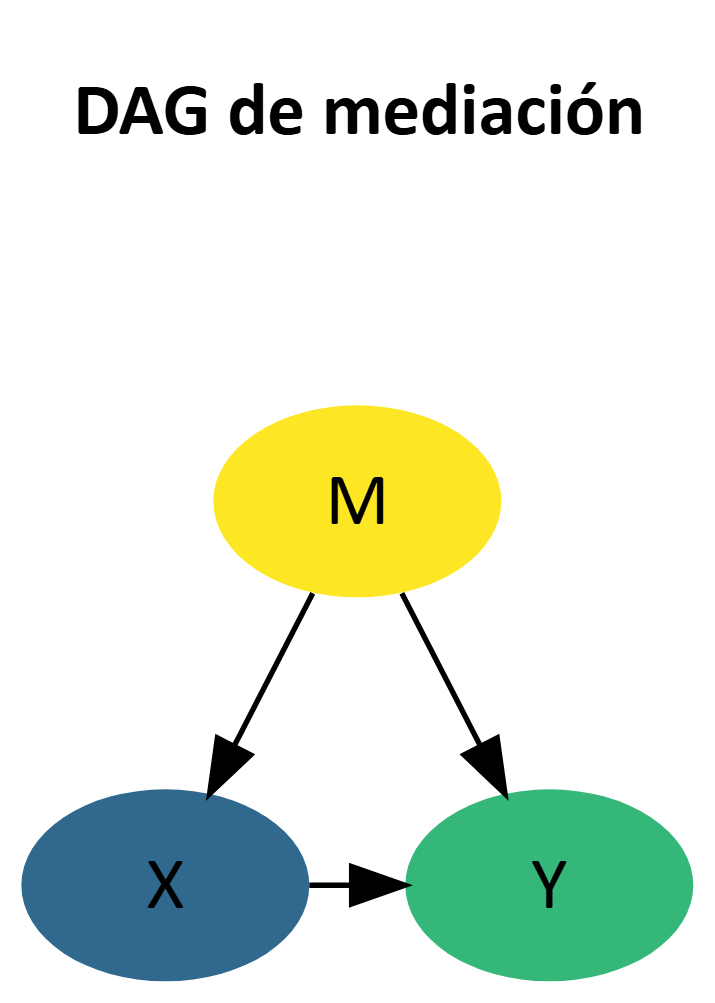
\includegraphics[width=5.5in,height=3.5in]{unidad_3/06_rol_variables_files/figure-latex/dot-figure-6.png}

El análisis de mediación descompone el efecto total en:

\begin{itemize}
\tightlist
\item
  \textbf{Efecto directo (ED)}: efecto de \(X\) sobre \(Y\) a través de
  todas las vías que no involucran \(M\)
\item
  \textbf{Efecto indirecto (EI)}: efecto de \(X\) sobre \(Y\) que opera
  a través de \(M\)
\item
  \textbf{Efecto total} = ED + EI
\end{itemize}

Si incluimos \(M\) como covariable en un modelo que busca estimar el
efecto total de \(X\) sobre \(Y\), bloquearemos el camino
\(X \rightarrow M \rightarrow Y\) y subestimaremos el efecto de la
exposición.

Un ejemplo lo podemos observar analizando este estudio ecológico, donde
se preguntan por el efecto del porcentaje de hogares con acceso a
espacios verdes (por municipio) sobre la tasa de mortalidad por
enfermedad cardiovascular (por 100.000 hab.)

Cuentan con otras variables que consideraron, entre las cuales, tienen
la proporción de población con actividad física regular.

{\def\LTcaptype{none} % do not increment counter
\begin{longtable}[]{@{}ccccccc@{}}
\toprule\noalign{}
\endhead
\bottomrule\noalign{}
\endlastfoot
~ & \multicolumn{3}{c}{%
mortalidad ev} & \multicolumn{3}{c@{}}{%
mortalidad ev} \\
Predictors & Estimates & CI & p & Estimates & CI & p \\
(Intercept) & 357.61 & 343.40~--~371.81 & \textbf{\textless0.001} &
367.97 & 356.27~--~379.67 & \textbf{\textless0.001} \\
espverde & -2.20 & -2.52~--~-1.87 & \textbf{\textless0.001} & -0.78 &
-1.21~--~-0.34 & \textbf{0.001} \\
actfis & & & & -2.35 & -2.92~--~-1.78 & \textbf{\textless0.001} \\
Observations & \multicolumn{3}{l}{%
120} & \multicolumn{3}{l@{}}{%
120} \\
R\textsuperscript{2} / R\textsuperscript{2} adjusted &
\multicolumn{3}{l}{%
0.602 / 0.599} & \multicolumn{3}{l@{}}{%
0.745 / 0.741} \\
\end{longtable}
}

Llegamos a estos resultados, hipotetizando en nuestro modelo teórico que
los espacios verdes reducen la mortalidad cardiovascular parcialmente a
través de facilitar la actividad física, pero también por vías directas
(reducción de estrés, calidad del aire, cohesión social). Razonar con
este modelo teórico, explica porque el coeficiente de espacios verdes
cambia al incluirla. Es decir, que el efecto total de espacios verdes
pasa de -2,20 a -0,78, es decir de un efecto total a un efecto directo
ante la presencia de actividad fisica.

Por lo tanto, si una variable es mediadora, no debe incluirse en el
modelo cuando se busca el efecto total. Para estimar el efecto
indirecto, se utilizan métodos de análisis de mediación (p.~ej.,
producto de coeficientes con bootstrap o modelos de ecuaciones
estructurales que exceden los alcances de este curso).

\section{Variable colisionadora}\label{variable-colisionadora}

Una variable \(C\) es colisionadora (o collider en inglés), si es una
consecuencia común de \(X\) e \(Y\) (o de causas de \(X\) e \(Y\)).

\protect\phantomsection\label{fig5}
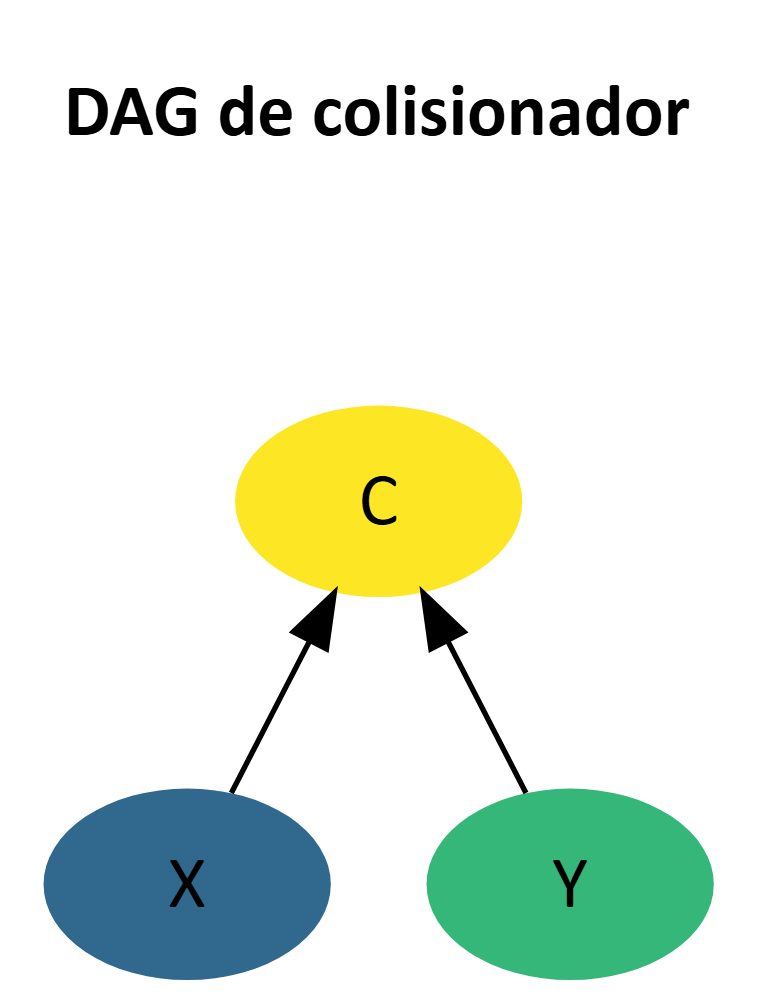
\includegraphics[width=5.5in,height=3.5in]{unidad_3/06_rol_variables_files/figure-latex/dot-figure-5.png}

A diferencia del confusor, el camino a través de un colisionador está
naturalmente bloqueado. La asociación espuria se crea cuando
condicionamos o controlamos por el colisionador: al incluirlo en el
modelo, restringir la muestra, o seleccionar participantes basándonos en
él, podemos generar una asociación artificial. Esto se llama sesgo de
colisionador (usualmente conocido como \emph{collider bias}, en inglés).

Es consecuencia generalmente de un sesgo de selección y se suele
manifestar en estudios de base hospitalaria (sesgo de Berkson), en
estudios longitudinales, si el abandono depende de la exposición y de
covariables del desenlace (pérdida no aleatoria) y en estudios con sesgo
de supervivencia (análisis de los supervivientes). Ver Holmberg y
Andersen (2022)

El ejemplo clásico es el de Berkson: Imaginemos un hospital que atiende
pacientes con dos enfermedades, enfermedad cardiovascular (CV) y
diabetes. La hospitalización actúa como colisionador. Supongamos que en
la población general la enfermedad CV y la diabetes son independientes
(no hay relación causal entre ellas). Sin embargo, si restringimos
nuestro análisis solo a pacientes hospitalizados, podríamos observar una
asociación negativa entre las dos. Quienes tienen enfermedad CV parecen
tener menos diabetes que el resto, y viceversa. Esta asociación es
completamente artificial (un artefacto del diseño). ¿Por qué? Porque la
hospitalización es consecuencia de tener al menos una de las dos
condiciones. Al condicionar sobre ``estar hospitalizado'', conectamos
artificialmente las dos enfermedades.

Otro ejemplo, que podemos ver en los datos, es el de una investigación
sobre el efecto del consumo de sodio (exposición) en la presión arterial
sistólica (desenlace). La recolección de datos incluye la edad y la
proteinuria (presencia de proteína en la orina).

{\def\LTcaptype{none} % do not increment counter
\begin{longtable}[]{@{}cccccccccc@{}}
\toprule\noalign{}
\endhead
\bottomrule\noalign{}
\endlastfoot
~ & \multicolumn{3}{c}{%
presion} & \multicolumn{3}{c}{%
presion} & \multicolumn{3}{c@{}}{%
presion} \\
Predictors & Estimates & CI & p & Estimates & CI & p & Estimates & CI &
p \\
(Intercept) & 119.42 & 117.22~--~121.62 & \textbf{\textless0.001} &
-0.31 & -1.11~--~0.49 & 0.445 & -0.09 & -0.47~--~0.28 & 0.634 \\
sodio & 3.96 & 3.37~--~4.55 & \textbf{\textless0.001} & 1.04 &
0.98~--~1.10 & \textbf{\textless0.001} & -0.90 & -0.97~--~-0.83 &
\textbf{\textless0.001} \\
edad & & & & 2.00 & 1.99~--~2.02 & \textbf{\textless0.001} & 0.42 &
0.36~--~0.47 & \textbf{\textless0.001} \\
proteinuria & & & & & & & 0.40 & 0.38~--~0.41 &
\textbf{\textless0.001} \\
Observations & \multicolumn{3}{l}{%
1000} & \multicolumn{3}{l}{%
1000} & \multicolumn{3}{l@{}}{%
1000} \\
R\textsuperscript{2} / R\textsuperscript{2} adjusted &
\multicolumn{3}{l}{%
0.150 / 0.149} & \multicolumn{3}{l}{%
0.991 / 0.991} & \multicolumn{3}{l@{}}{%
0.998 / 0.998} \\
\end{longtable}
}

Vemos tres modelos, el primero es un modelo del efecto bruto del consumo
de sodio sobre la presión arterial, el segundo incluye la edad y
manifiesta un efecto confusor sobre la relación y el tercer modelo, al
incluir proteinuria, manfiesta el efecto colisionador (ver que el
coeficiente de sodio invierte su signo).

El DAG de este ejemplo, muestra que tanto el consumo elevado de sodio
como la presión arterial alta son causas de la proteinuria, por lo que
es un error controlar por esa variable. (Luque-Fernandez et~al. (2019))

\section{Interacción o modificación de
efecto}\label{interacciuxf3n-o-modificaciuxf3n-de-efecto}

MacMahon (1972) definió la interacción de la siguiente manera:

\begin{tcolorbox}[enhanced jigsaw, arc=.35mm, bottomrule=.15mm, breakable, colback=white, colframe=quarto-callout-important-color-frame, left=2mm, leftrule=.75mm, opacityback=0, rightrule=.15mm, toprule=.15mm]
\begin{minipage}[t]{5.5mm}
\textcolor{quarto-callout-important-color}{\faExclamation}
\end{minipage}%
\begin{minipage}[t]{\textwidth - 5.5mm}

\emph{``Cuando la incidencia de la enfermedad en presencia de dos o más
factores de riesgo difiere de la incidencia que sería previsible por sus
efectos individuales''}

\end{minipage}%
\end{tcolorbox}

Esto puede manifestarse como:

\begin{itemize}
\item
  \textbf{Sinergismo (interacción positiva):} El efecto combinado es
  mayor que la suma de sus efectos individuales.
\item
  \textbf{Antagonismo (interacción negativa):} El efecto combinado es
  menor.
\end{itemize}

La modificación del efecto ocurre cuando la magnitud de la asociación
entre la exposición (\(X\)) y el resultado (\(Y\)) varía según los
niveles de una tercera variable (\(I\)).

No es un sesgo ---es una característica real del fenómeno--- y no debe
eliminarse sino \emph{describirse} (es decir, incluirla en el modelo e
informar en los resultados de forma estratificada)

Para quienes tengan interés en profundizar el tema, pueden leer el
artículo:

➡️ De Irala, J., et al.~(2001). ¿Qué es una variable modificadora del
efecto? \emph{Medicina Clínica}, \emph{117}(8), 297--302.
\url{https://doi.org/10.1016/S0025-7753(01)72092-1}

Para identificar la interacción en regresión lineal múltiple, se
incluyen términos de interacción (\(X * I\)), que representan una nueva
variable con efectos multiplicativos. El término de interacción implica
el exceso de la variabilidad de los datos que no puede ser explicada por
la suma de las variables consideradas.

En cursos anteriores de Epidemiología se estudió que, frente a un
modificador de efecto (\(I\)) lo más adecuado era presentar las medidas
de asociación según los estratos formados por las categorías de la
variable \(I\) (no estimar una medida ajustada para ambos estratos, como
se hace en caso de variables confusoras).

Un ejemplo similar al recién mostrado para la confusión, pero para la
interacción podría ser:

\begin{center}
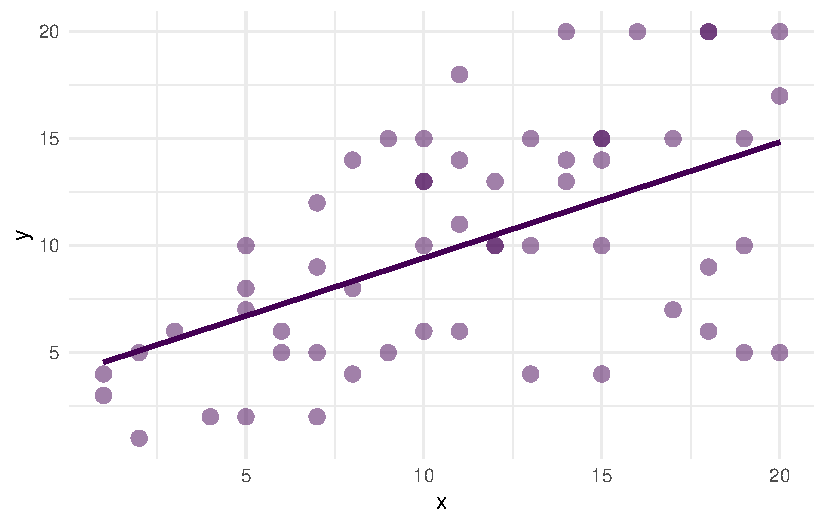
\includegraphics[width=0.85\linewidth,height=\textheight,keepaspectratio]{unidad_3/06_rol_variables_files/figure-pdf/fig6-1.pdf}
\end{center}

\[
\hat{y} = \beta_0 + \beta_1x_1 + \epsilon
\]

Partimos de esta relación entre \(X\) e \(Y\) representada por la recta
de la ecuación con los valores de la siguiente tabla:

\begin{verbatim}

Call:
lm(formula = y ~ x, data = datos_int)

Residuals:
    Min      1Q  Median      3Q     Max 
-9.8410 -3.8804  0.3709  3.2871  8.4102 

Coefficients:
            Estimate Std. Error t value Pr(>|t|)    
(Intercept)   4.0035     1.4065   2.847   0.0062 ** 
x             0.5419     0.1132   4.789 1.31e-05 ***
---
Signif. codes:  0 '***' 0.001 '**' 0.01 '*' 0.05 '.' 0.1 ' ' 1

Residual standard error: 4.554 on 55 degrees of freedom
Multiple R-squared:  0.2943,    Adjusted R-squared:  0.2814 
F-statistic: 22.93 on 1 and 55 DF,  p-value: 1.307e-05
\end{verbatim}

El intercepto (\(\beta_0\)) es de 4,0 y el coeficiente \(\beta_1\)
(pendiente) significativo de 0,54.

Ahora incorporemos la covariable \(Z\), con categorías \textbf{A} y
\textbf{B}, que sospechamos tiene un rol de interacción.

\begin{center}
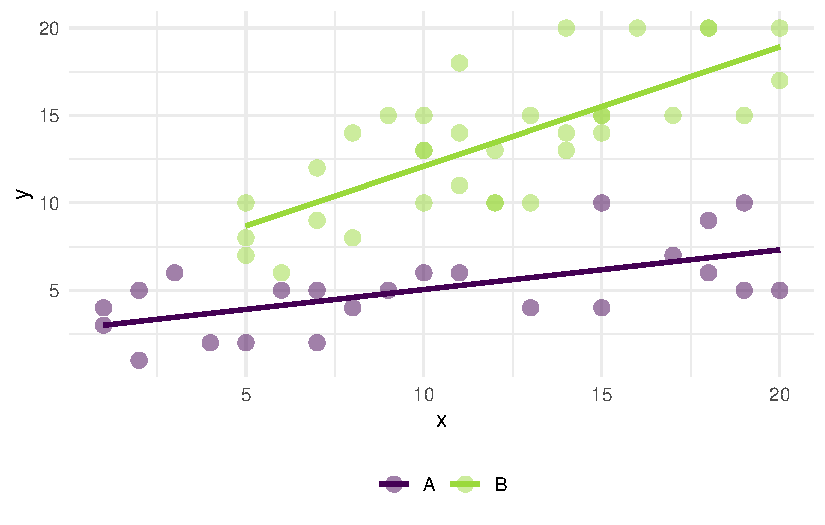
\includegraphics[width=0.85\linewidth,height=\textheight,keepaspectratio]{unidad_3/06_rol_variables_files/figure-pdf/fig7-1.pdf}
\end{center}

El gráfico de dispersión muestra que hay una diferencia entre las rectas
de regresión que tienen distintas pendientes según el valor de \(Z\).
Esa diferencia no es aditiva y pasa a ser multiplicativa y da lugar a la
ecuación:

\[
\hat{y} = \beta_0 + \beta_1x_1 + \beta_2x_2 + \beta_3x_1x_2 + \epsilon
\]

Visto en resultados de consola:

\begin{verbatim}

Call:
lm(formula = y ~ x * z, data = datos_int)

Residuals:
    Min      1Q  Median      3Q     Max 
-4.1427 -1.8739 -0.4598  1.3199  5.2230 

Coefficients:
            Estimate Std. Error t value Pr(>|t|)    
(Intercept)  2.77269    0.91587   3.027 0.003804 ** 
x            0.22708    0.07719   2.942 0.004830 ** 
zB           2.49329    1.51850   1.642 0.106522    
x:zB         0.45574    0.12213   3.732 0.000465 ***
---
Signif. codes:  0 '***' 0.001 '**' 0.01 '*' 0.05 '.' 0.1 ' ' 1

Residual standard error: 2.364 on 53 degrees of freedom
Multiple R-squared:  0.8168,    Adjusted R-squared:  0.8064 
F-statistic: 78.75 on 3 and 53 DF,  p-value: < 2.2e-16
\end{verbatim}

El término de interacción es significativo, aunque la variable \(I\) por
sí misma no lo sea, lo que implica que la significancia se encuentra
asociada específicamente a uno de los niveles de \(I\) (en este caso, la
categoría B). Dado que no es posible separar los niveles de \(I\), esta
variable debe permanecer en el modelo. Además, la inclusión del término
de interacción mejora el \(R^2\) ajustado del modelo, que pasa de 0,28 a
0,81. Esto demuestra que, cuando la interacción es significativa, la
significancia estadística de los efectos simples de las variables \(X\)
e \(I\) se vuelve habitualemente menos relevante.

El modelo ajustado para \(Y\) es el siguiente:

\begin{itemize}
\tightlist
\item
  Para \(I = A\):
\end{itemize}

\[
y = 2,77 + 0,23 x
\]

\begin{itemize}
\tightlist
\item
  Para \(I = B\):
\end{itemize}

\[
y = 2,77 + 0,23x +2,49 + 0,46x 
\]

Esto muestra una interacción sinérgica entre la categoría B de la
variable \(I\) y la variable \(X\), reflejada en el efecto sobre \(Y\).
La pendiente de la recta para \(I = B\) es mayor que para \(I = A\), lo
que indica que el efecto de \(X\) sobre \(Y\) varía según el nivel de
\(I\).

\subsection{Limitaciones de los términos de
interacción}\label{limitaciones-de-los-tuxe9rminos-de-interacciuxf3n}

Aunque el análisis de interacción en modelos lineales generales es una
herramienta útil para explorar relaciones complejas entre variables, es
importante ser consciente de sus limitaciones y asumirlas en el diseño,
análisis e interpretación de los resultados. Entre ellas encontramos:

\begin{itemize}
\item
  \textbf{Linealidad y Simplicidad del Modelo:} El modelo lineal general
  asume relaciones lineales entre las variables, pero las interacciones
  a veces no muestran linealidad.
\item
  \textbf{Sobreajuste en Modelos con Múltiples Interacciones:} La
  inclusión de muchos términos de interacción, puede sobreajustar el
  modelo y dificultar su interpretación y generalización.
\item
  \textbf{Colinealidad:} La colinealidad entre las variables
  independientes puede ser exacerbada al incluir términos de
  interacción, lo que dificultaría la identificación de relaciones
  significativas.
\item
  \textbf{Pérdida de Potencia Estadística:} Al incluir términos de
  interacción, el número de parámetros a estimar aumenta, reduciendo los
  grados de libertad y pudiendo disminuir la potencia estadística.
\item
  \textbf{Dificultades en la Interpretación:} Los coeficientes de
  interacción pueden ser difíciles de interpretar, especialmente cuando
  las variables son continuas.
\item
  \textbf{Heterogeneidad de Efectos:} Los términos de interacción pueden
  no capturar variaciones en los efectos entre subgrupos específicos.
\item
  \textbf{Errores de Especificación del Modelo:} Si las interacciones
  relevantes no se incluyen o se modelan incorrectamente, el modelo
  puede estar mal especificado.
\item
  \textbf{Sensibilidad a la Codificación de las Variables:} La
  codificación de variables categóricas puede influir en la
  interpretación de los coeficientes de interacción.
\end{itemize}

\section{Resumen: ¿Qué ajustar y que
no?}\label{resumen-quuxe9-ajustar-y-que-no}

{\def\LTcaptype{none} % do not increment counter
\begin{longtable}[]{@{}
  >{\raggedright\arraybackslash}p{(\linewidth - 8\tabcolsep) * \real{0.0927}}
  >{\raggedright\arraybackslash}p{(\linewidth - 8\tabcolsep) * \real{0.1060}}
  >{\raggedright\arraybackslash}p{(\linewidth - 8\tabcolsep) * \real{0.1589}}
  >{\raggedright\arraybackslash}p{(\linewidth - 8\tabcolsep) * \real{0.2781}}
  >{\raggedright\arraybackslash}p{(\linewidth - 8\tabcolsep) * \real{0.3642}}@{}}
\toprule\noalign{}
\begin{minipage}[b]{\linewidth}\raggedright
Variable
\end{minipage} & \begin{minipage}[b]{\linewidth}\raggedright
Estructura DAG
\end{minipage} & \begin{minipage}[b]{\linewidth}\raggedright
Ajuste
\end{minipage} & \begin{minipage}[b]{\linewidth}\raggedright
Si no ajustás
\end{minipage} & \begin{minipage}[b]{\linewidth}\raggedright
Si ajustas innecesariamente
\end{minipage} \\
\midrule\noalign{}
\endhead
\bottomrule\noalign{}
\endlastfoot
Confusora & X \textless-- Z --\textgreater{} Y & Sí & Sesgo de confusión
& --- \\
Mediadora & X --\textgreater{} M --\textgreater{} Y & Depende del
objetivo & Se estima efecto total & Sesgo por sobre-ajuste;
subestimación del efecto total \\
Colisionadora & X --\textgreater{} C \textless-- Y & No & Sin problema
(camino bloqueado) & Sesgo de colisionador; asociación espuria \\
Interacción & I --\textgreater{} (X --\textgreater{} Y) & Incluir como
interaccón & Efecto promediado (heterogeneidad oculta) & --- \\
\end{longtable}
}

\section{Teoría vs algoritmo}\label{teoruxeda-vs-algoritmo}

Muchos algoritmos de selección automática de variables (como
\emph{stepwise regression}) incluyen toda variable que mejore
\emph{``matemáticamente''} el ajuste de un modelo o tiene un p-valor
bajo. No distingue que rol juega esa variable, si se trata de un
mediador o de un colisionador, de un confusor o es modificadora de
efecto.

Ante las preguntas, ¿Por qué en estos casos el criterio estadístico
puede fallar en identificar el modelo correcto? ¿Qué nos dice esto sobre
la importancia de construir un DAG antes de tocar los datos?, la
respuesta es que el modelo estadístico no sabe de epidemiología.

Según Almeida Filho y Barreto (2011), \emph{``Es verdad que las técnicas
utilizadas para la atribución de valores numéricos al grado de certeza
de que las variables se encuentran asociadas son eminentemente
estadísticas. Sin embargo, en el campo de la Epidemiología, la
estadística no habla por sí sola. Le corresponde al epidemiólogo
analizar los resultados obtenidos a la luz del conocimiento
epidemiológico acumulado, el contexto en el cual el fenómeno analizado
es parte y las características propias, cualitativas, asumidas por el
fenómeno en su especificidad temporal y espacial. Es decir, más que
significancia estadística, la interpretación de los datos debe buscar
establecer la''significancia epidemiológica'' de los hallazgos. Esa es
la esencia del análisis epidemiológico.''}

\section*{Referencias}\label{referencias-16}
\addcontentsline{toc}{section}{Referencias}

\markright{Referencias}

\chapter{Regresión lineal
múltiple}\label{regresiuxf3n-lineal-muxfaltiple}

\section{Introducción}\label{introducciuxf3n-16}

Los modelos de Regresión Lineal Múltiple (RLM) son herramientas
estadísticas ampliamente utilizadas cuando la variable dependiente es
continua y existen dos o más variables independientes, que pueden ser
tanto continuas como categóricas. En el caso de las covariables
categóricas, estas pueden ser dicotómicas, ordinales o tener múltiples
niveles.

Al igual que la Regresión Lineal Simple (RLS), que permite estimar el
efecto bruto de una variable independiente sobre la variable
dependiente, la RLM nos permite conocer el efecto conjunto de dos o más
variables independientes (\(X_1\), \(X_2\),\ldots{}\(X_k\)) sobre la
variable dependientea (\(Y\)). De esta manera, la RLM nos permite:

\begin{itemize}
\item
  \textbf{Analizar la dirección y fuerza de la asociación} entre la
  variable dependiente y las variables independientes.
\item
  \textbf{Identificar las variables independientes importantes} en la
  predicción o explicación de la variable dependiente.
\item
  \textbf{Describir la relación entre una o más variables
  independientes}, controlando la confusión.
\item
  \textbf{Detectar interacciones}, es decir, cómo cambia la relación
  entre la variable dependiente y una variable independiente según el
  nivel de otra variable independiente.
\end{itemize}

El modelo estadístico de la RLS que expresa la relación entre \(X\) e
\(Y\) es:

\[
Y = \beta_0 + \beta_1X_1
\]

Este modelo se representa gráficamente como una recta de ajuste en un
plano bidimensional (dos dimensiones).

Por otro lado, el modelo estadístico de la RLM es:

\[
Y = \beta_0 + \beta_1X_1 + \beta_2X_2 + ...+\beta_kX_k  
\]

Donde \(\beta_0\), \(\beta_1\), \(\beta_2\),\ldots,\(\beta_k\) son los
parámetros de la regresión. Para cada combinación de valores de \(X_1\),
\(X_2\),\ldots{}\(X_k\) existe una distribución \(Y\) cuya
\textbf{media} es una función lineal de \(X_1\), \(X_2\),\ldots,
\(X_k\).

\begin{center}
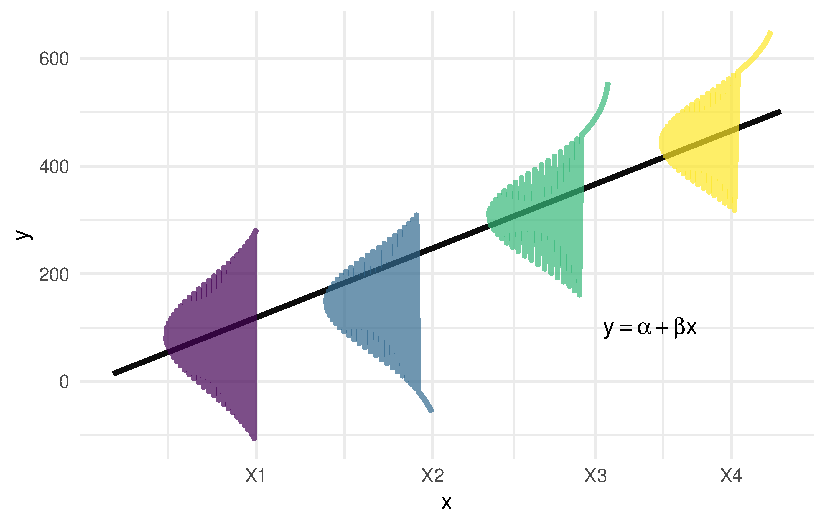
\includegraphics[width=0.85\linewidth,height=\textheight,keepaspectratio]{unidad_3/07_reg_lineal_multiple_files/figure-pdf/fig1-1.pdf}
\end{center}

La representación gráfica de la recta de ajuste en la regresión lineal
múltiple se realiza en un espacio de dimensión \(K + 1\), donde \(K\) es
el número de variables independientes. En el caso de la regresión lineal
simple (RLS), la relación se puede representar fácilmente en un plano
bidimensional (2D). Sin embargo, a medida que aumentamos el número de
variables independientes, la representación gráfica se vuelve más
compleja, ya que requerimos más dimensiones, lo que dificulta visualizar
el modelo en el espacio.

En el caso puntual que el modelo tuviera 2 variables independientes, la
ecuación sería:

\[
Y = \beta_0 + \beta_1 X_1 + \beta_2X_2
\]

En este caso, la relación podría representarse en un plano
tridimensional (3D), donde los ejes corresponden a \(X_1\), \(X_2\) y la
variable dependiente \(Y\). En este plano, la superficie de ajuste es un
plano que describe la relación entre las tres variables, y la
orientación de dicho plano estará determinada por los coeficientes
\(\beta_1\) y \(\beta_2\).

\begin{center}
\pandocbounded{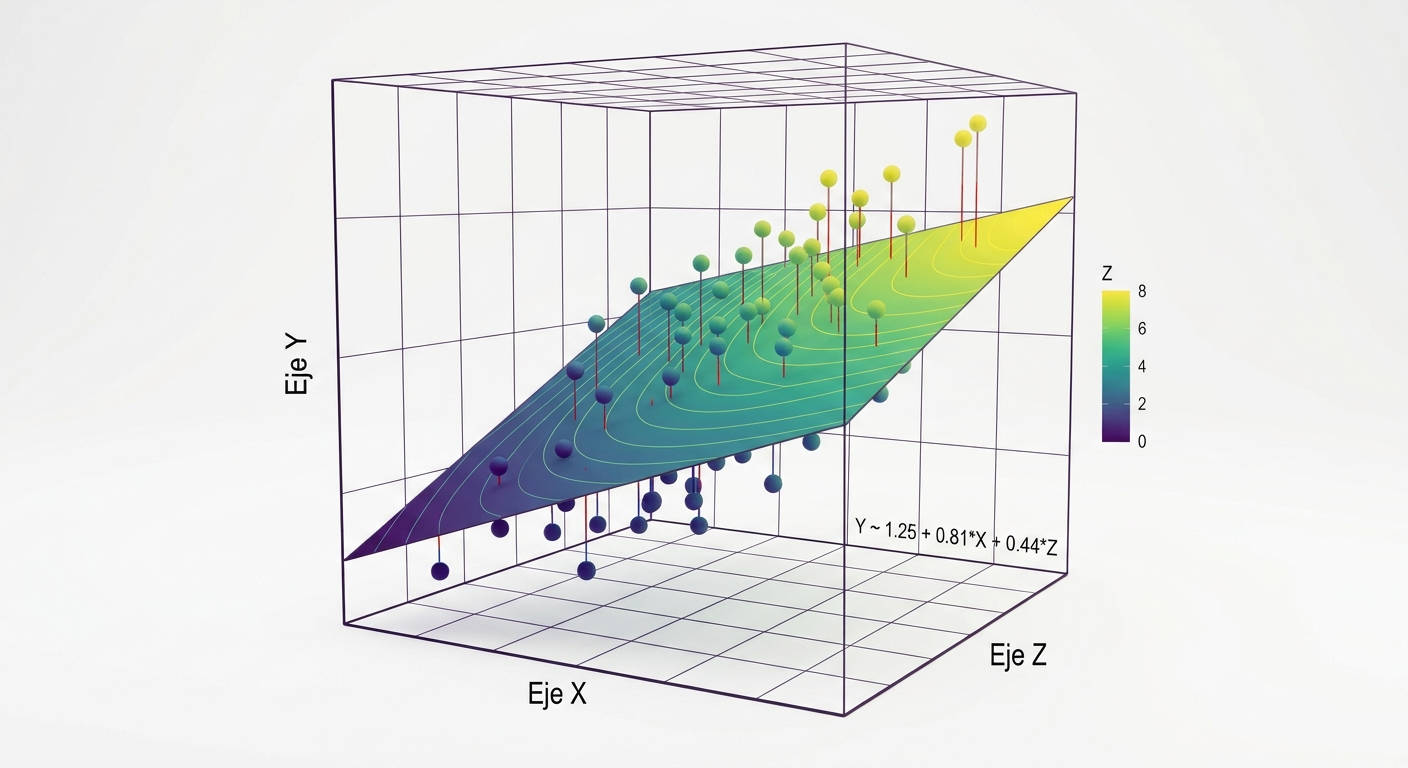
\includegraphics[keepaspectratio]{unidad_3/images/rlm.jpg}}
\end{center}

En forma similar a la RLS, la interpretación de cada parámetro \(\beta\)
de la regresión es:

\begin{itemize}
\item
  \(\beta_0\): es el valor esperado de \(Y\) cuando todas las otras
  variables son iguales a cero.
\item
  \(\beta_1\) es la pendiente a lo largo del eje \(X_1\) y representa el
  cambio esperado en la respuesta por unidad de cambio en \(X_1\) a
  valores constantes de \(X_2\).
\item
  \(\beta_2\) es la pendiente a lo largo del eje \(X_2\) y representa el
  cambio esperado en la respuesta por unidad de cambio en \(X_2\) a
  valores constantes de \(X_1\).
\end{itemize}

\section{Presupuestos del modelo de
RLM}\label{presupuestos-del-modelo-de-rlm}

\subsection{Independencia}\label{independencia}

Las observaciones \(Y_i\) son independientes unas de otras: el efecto de
\(X_1\) sobre la respuesta media no depende de \(X_2\) y viceversa,
siempre y cuando no exista interacción. Cuando existe interacción entre
\(X_1\) e \(X_2\) , el efecto de \(X_1\) sobre la respuesta media de
\(Y\) depende \(X_2\) y viceversa (\(X_1\) e \(X_2\) no son
independientes cuando existe interacción).

\subsection{Linealidad}\label{linealidad}

Para cada combinación de valores de las variables independientes
(\(X_1\), \(X_2\),\ldots, \(X_k\)) el valor medio de \(Y\) es función
lineal de \(X_1\), \(X_2\),\ldots,\(X_k\).. La linealidad se define en
relación a los coeficientes de la regresión, por lo tanto el modelo
puede incluir términos cuadráticos e interacciones

\begin{itemize}
\tightlist
\item
  Modelo con interacción
\end{itemize}

\[
Y = \beta_0X_1 + \beta_2X_2 + \beta_3X_1X_2 
\]

\begin{itemize}
\tightlist
\item
  Modelo con términos cuadráticos
\end{itemize}

\[
Y = \beta_0 + \beta_1X_1 + \beta_2X_2 + \beta_3X_1^2 + \beta_4X_2^2 
\]

\subsection{Homocedasticidad}\label{homocedasticidad-2}

la varianza de \(Y\) para los distintos valores de \(X_1\),
\(X_2\),\ldots,\(X_k\) se mantiene constante.

\subsection{Normalidad}\label{normalidad-2}

Los valores de \(Y\) tienen una distribución normal según los valores de
\(X_1\), \(X_2\), \(X_k\) , ésto nos permite realizar inferencias en
relación a los parámetros del modelo.

Al igual que en la RLS la estimación de los parámetros de la regresión
(coeficientes) se realiza mediante el \textbf{Método de los Mínimos
Cuadrados} \textbf{(MMC)}. El mismo consiste en adoptar como estimativas
de los parámetros de la regresión los valores que minimicen la suma de
los cuadrados de los residuos.

\[ 
\sum_{i=1}^{i=n}e_1^2=\sum_{i=1}^{i=n}(Y_i-\hat{Y_i})^2=\sum_{i=n}^{i=n}(Y_i-(\hat{\beta}_0+\hat{\beta}_1X_1+\dots+\hat{\beta}_kX_k))^2
\]

\section{Interpretación del modelo}\label{interpretaciuxf3n-del-modelo}

Comenzaremos aprendiendo cómo interpretar un modelo de regresión lineal
múltiple (RLM) antes de abordar su construcción. Para ilustrarlo,
observemos en detalle la salida de R para un modelo de RLM en el que
modelamos la variable \texttt{V23}, en función de las variables
\texttt{V10}, \texttt{V11}, \texttt{V12}, \texttt{V14}, \texttt{V15},
\texttt{V17}, \texttt{V18} y \texttt{V24}.

\begin{verbatim}

Call:
lm(formula = V23 ~ ., data = data)

Residuals:
     Min       1Q   Median       3Q      Max 
-2.45958 -0.57136  0.05354  0.57868  2.25036 

Coefficients:
            Estimate Std. Error t value Pr(>|t|)  
(Intercept)  0.09504    0.09502   1.000   0.3199  
V10         -0.05189    0.09725  -0.534   0.5950  
V11         -0.11508    0.09711  -1.185   0.2391  
V12         -0.08137    0.09151  -0.889   0.3763  
V14         -0.16411    0.09738  -1.685   0.0954 .
V15         -0.03240    0.10283  -0.315   0.7534  
V17         -0.04053    0.09040  -0.448   0.6550  
V18          0.14425    0.09456   1.525   0.1306  
V24         -0.04953    0.08940  -0.554   0.5809  
---
Signif. codes:  0 '***' 0.001 '**' 0.01 '*' 0.05 '.' 0.1 ' ' 1

Residual standard error: 0.9081 on 91 degrees of freedom
Multiple R-squared:  0.09027,   Adjusted R-squared:  0.0103 
F-statistic: 1.129 on 8 and 91 DF,  p-value: 0.3518
\end{verbatim}

En la salida obtenida, encontramos varios términos clave para
interpretar:

\begin{itemize}
\item
  \texttt{Estimate}: muestra los coeficientes estimados (\(\beta\)) para
  el intercepto (\(\beta_0\)) y para cada una de las variables
  explicativas (\(\beta_i\)).
\item
  \texttt{Std.\ Error}: el error estándar de cada coeficiente estimado
  \(\beta\).
\item
  \texttt{t-value}: los valores del test \(t\) para cada coeficiente,
  que evalúan si los coeficientes son significativamente diferentes de
  cero.
\item
  \texttt{Pr(\textgreater{}\textbar{}t\textbar{})}: los valores \(p\)
  asociados a los test \(t\) para cada coeficiente.
\item
  \texttt{Residual\ standard\ error}: el error estándar de los
  residuales.
\item
  \texttt{Multiple\ R-squared}: el coeficiente de determinación \(R^2\)
  múltiple, que indica qué proporción de la variabilidad de la variable
  dependiente es explicada por el modelo.
\item
  \texttt{Adjusted\ R-squared}: el coeficiente de determinación
  ajustado, que penaliza por la inclusión de variables que no mejoran el
  modelo.
\item
  \texttt{F-statistic}: el resultado del test \(F\) global, que evalúa
  la significancia del modelo en su conjunto, junto con su valor \(p\).
\end{itemize}

\subsection{Test F parcial}\label{test-f-parcial}

En un modelo de regresión, la estimación de los coeficientes se realiza
partiendo de una muestra, lo que implica que diferentes muestras pueden
generar distintos valores de los parámetros. El test F parcial evalúa la
siguiente hipótesis:

\[
H_0 = \beta_1 = \beta_2 = ... \beta_n = 0  \\H_1 = \exists\beta_i \neq 0
\]

Donde \(H_0\) indica que todos los coeficientes de las variables
independientes son cero, y \(H_1\) implica que al menos uno de los
coeficientes es diferente de cero. Este test evalúa la contribución de
cada variable al modelo, es decir, si la inclusión de esa variable
mejora significativamente la explicación de la variabilidad de \(Y\). En
modelos de regresión lineales generalizados (GLM), el test de Wald
cumple esta misma función, mientras que en los modelos de regresión
lineales múltiplos, el test \(F\) parcial cumple el mismo rol.

\subsection{Varianza residual}\label{varianza-residual}

Al igual que en la
\hyperref[regresiuxf3n-lineal-simple]{\textbf{regresión lineal simple}}y
el \hyperref[anuxe1lisis-de-la-varianza-anova]{\textbf{análisis de la
varianza (ANOVA)}}, podemos descomponer la variabilidad de la variable
dependiente \(Y\) en dos componentes:

\begin{enumerate}
\def\labelenumi{\arabic{enumi}.}
\item
  Variabilidad explicada por el modelo.
\item
  Variabilidad \textbf{no explicada} por el modelo, atribuida a factores
  aleatorios.
\end{enumerate}

Matemáticamente, esto se expresa como:

\[
Variabilidad \ total = Variabilidad \ regresión \ + \ Variabilidad \ residual
\]

De manera equivalente, la suma de cuadrados totales (SCT) se descompone
en la suma de cuadrados de la regresión (SCR) y la suma de cuadrados
residuales (SCE):

\[
\sum (y_i-\bar{y})^2 = \sum (\hat{y}-\bar{y})^2 + \sum (y_i -\hat{y}_i)^2
\\
SCT = SCR + SCE
\]

A continuación, mostramos cómo estos términos se distribuyen entre los
grados de libertad y se obtienen los cuadrados medios correspondientes:

{\def\LTcaptype{none} % do not increment counter
\begin{longtable}[]{@{}lll@{}}
\toprule\noalign{}
& Grados de libertad & CM \\
\midrule\noalign{}
\endhead
\bottomrule\noalign{}
\endlastfoot
SCT & n-1 & CMT = SCT/n-1 \\
SCR & k-1 & CMR = SCR/k-1 \\
SCE & n-k-1 & CME = SCE/n-k-1 \\
\end{longtable}
}

\subsection{Test F global}\label{test-f-global}

El test \(F\) global compara el modelo de regresión ajustado con el
modelo nulo (sin variables independientes) y evalúa el efecto conjunto
de todas las variables independientes. Su fórmula es:

\[ 
F = CMR/CME 
\\ 
gl = (k -1, n - k - 1) 
\]

\subsection{Coeficiente de
determinación}\label{coeficiente-de-determinaciuxf3n}

Al igual de lo que aprendimos en la RLS la bondad de ajuste del modelo
de RLM se valora con el coeficiente de determinación (\(R^2\)), que nos
dice qué proporción de la variabilidad de \(Y\) es explicada por los
coeficientes de la regresión del modelo en estudio. Su valor se calcula
como:

\[ 
R^2 = \frac{SCT-SCE}{SCT}=\frac{SCR}{SCT} 
\]

Sin embargo, al agregar más variables al modelo, \(R^2\) siempre mejora,
incluso si la nueva variable no mejora sustancialmente el modelo. Este
fenómeno se debe a que \(R^2\) solo refleja la proporción de
variabilidad explicada, pero no penaliza la inclusión de variables que
no aportan al modelo.

Por esta razón, se utiliza el \(R^2\) ajustado, que corrige el \(R^2\)
penalizando la inclusión de variables que no aportan significativamente:

\[ 
R^2_a = 1 - \bigg [ \frac{n-1}{n-(k+1)}\bigg]\frac{SCE}{SCT}=1-\bigg[\frac{n-1}{n-(k+1)}\bigg](1-R^2)  
\]

Como el término \(1 - R^2\) es constante y \(n\) es mayor que \(k\), a
medida que agregamos variables, el cociente entre paréntesis crece, lo
que hace que la penalización por agregar variables no significativas
también aumente. Esto hace que el \(R^2\) ajustado sea una medida más
fiable de la calidad del modelo.

\begin{tcolorbox}[enhanced jigsaw, arc=.35mm, bottomrule=.15mm, breakable, colback=white, colframe=quarto-callout-warning-color-frame, left=2mm, leftrule=.75mm, opacityback=0, rightrule=.15mm, toprule=.15mm]
\begin{minipage}[t]{5.5mm}
\textcolor{quarto-callout-warning-color}{\faExclamationTriangle}
\end{minipage}%
\begin{minipage}[t]{\textwidth - 5.5mm}

Cuando tenemos que elegir el mejor modelo será necesario utilizar
distintos criterios para compararlos y basar nuestra decisión en elegir
el modelo que mejor explique la variación de \(Y\) con el menor número
de variables independientes, el modelo más simple y efectivo, también
llamado el modelo más \textbf{parsimonioso}.

\end{minipage}%
\end{tcolorbox}

\section{\texorpdfstring{Variables
\emph{dummy}}{Variables dummy}}\label{variables-dummy}

En los modelos de regresión, podemos incluir tanto variables
cuantitativas como variables categóricas. Las variables categóricas
pueden ser dicotómicas (por ejemplo, sexo: femenino/masculino; hábito de
fumar: sí/no) o tener más de dos categorías (por ejemplo, grupo
sanguíneo, religión, color de ojos).

Para modelar las variables categóricas, cada categoría se transforma en
una variable dicotómica (binaria), con un número de categorías menos
uno. Es decir, para una variable con \(n\) categorías, se crearán
\(n-1\) variables \emph{dummy}, donde \(1\) indica la presencia de esa
categoría y \(0\) indica su ausencia. En estos casos, se selecciona como
grupo basal (o grupo de referencia) la categoría con el valor más bajo.

\subsubsection{Ejemplo para variable independiente
dicotómica}\label{ejemplo-para-variable-independiente-dicotuxf3mica}

Supongamos que tenemos una variable cualitativa dicotómica, como
``Hábito de Fumar'', que toma los valores 1 (si fuma) y 0 (si no fuma).
Si ajustamos un modelo con esta variable, la ecuación sería:

\[ 
Y = \beta_0+\beta_1F_1  
\]

Donde:

\begin{itemize}
\item
  \(Y\) es la variable dependiente.
\item
  \(\beta_0\) es el intercepto (valor basal de \(Y\) cuando el individuo
  no fuma).
\item
  \(\beta_1\) es el coeficiente asociado al hábito de fumar, que indica
  el cambio en \(Y\) cuando el individuo fuma (es decir, la diferencia
  entre el grupo de fumadores y no fumadores).
\end{itemize}

\subsubsection{Ejemplo para variable independiente con múltiples
categorías}\label{ejemplo-para-variable-independiente-con-muxfaltiples-categoruxedas}

Ahora, consideremos una variable ``Región'', que tiene tres categorías:
Noreste (NE), Norte (N) y Centro Oeste (CO). Para modelarla como
variables \emph{dummy}, la transformamos en dos variables: \(Re_1\) y
\(Re_2\), ya que hay \(n-1 = 3-1 = 2\) categorías \emph{dummy}.

La transformación de las categorías sería:

{\def\LTcaptype{none} % do not increment counter
\begin{longtable}[]{@{}lrr@{}}
\toprule\noalign{}
Región & RE1 & RE2 \\
\midrule\noalign{}
\endhead
\bottomrule\noalign{}
\endlastfoot
NE (basal) & 0 & 0 \\
N & 1 & 0 \\
CO & 0 & 1 \\
\end{longtable}
}

En este caso:

\begin{itemize}
\item
  \(Re_1 = 1\) si vive en el Norte, \(Re_1 = 0\) si vive en otra región.
\item
  \(Re_2 = 1\) si vive en el Centro Oeste, \(Re_2 = 0\) si vive en otra
  región.
\end{itemize}

Ahora imaginemos el modelo de regresión entre \(Y\) y la variable
\emph{``región''} (supongamos que \(Y\) es la Tasa de Mortalidad
Infantil):

\[ 
Y = \beta_0+\beta_1Re_1 + \beta_2Re_2 
\]

Para interpretar el modelo:

\begin{itemize}
\tightlist
\item
  Si el individuo vive en la región Norte (\(Re_1 = 1\) y \(Re_2 = 0\)),
  la ecuación se reduce a:
\end{itemize}

\[ 
Y=\beta_0+\beta_1Re_1  
\]

\begin{itemize}
\tightlist
\item
  Si el individuo vive en la región Centro Oeste (\(Re_1 = 0\) y
  \(Re_2 = 1\)), la ecuación sería:
\end{itemize}

\[ 
Y=\beta_0+\beta_2Re_2  
\]

\begin{itemize}
\tightlist
\item
  Si el individuo vive en la región Noreste (grupo basal, \(Re_1 = 0\) y
  \(Re_2 = 0\)), la ecuación se reduce a:
\end{itemize}

\[ 
Y=\beta_0 
\]

En este contexto, \(\beta_1\) y \(\beta_2\) nos estarán indicando cuánto
se modifica la TMI según consideremos la región Norte o Centro Oeste. El
coeficiente \(\beta_0\) es el valor basal medio de la TMI considerada en
la región Noreste

Las variables \emph{dummy} o indicadoras no tienen un significado por sí
solas, ya que su interpretación depende de cómo se comparan con el grupo
basal. Es importante que todas las categorías de la variable cualitativa
estén representadas en el modelo, y la inclusión de estas variables debe
ser contrastada en bloque, incluso si algunos de los tests \(F\)
parciales para una categoría no son significativos.

Además, al agregar una variable \emph{dummy} al modelo, esta incrementa
los grados de libertad de la regresión en función de la cantidad de
categorías de la variable. Por ejemplo, si una variable tiene \(n\)
categorías, se agregarán \(n-1\) variables \emph{dummy}, cada una con su
respectivo grado de libertad.

Cuando trabajamos en R, el lenguaje se encarga de construir las
variables \emph{dummy} automáticamente siempre que su estructura sea
\textbf{factor}. Los tipos de datos \textbf{factor} tienen una
estructura de niveles donde el primero de ellos es el de referencia.
Para modificar el nivel de referencia podemos utilizar las funciones
\texttt{relevel()} de R \texttt{base} o \texttt{fct\_relevel()} de
\texttt{tidyverse}.

\section{Estimación y predicción en modelos de
regresión}\label{estimaciuxf3n-y-predicciuxf3n-en-modelos-de-regresiuxf3n}

La regresión es una herramienta clave en los análisis tanto explicativos
como predictivos, y se utiliza de las siguientes maneras:

\begin{enumerate}
\def\labelenumi{\arabic{enumi}.}
\item
  \textbf{Con fines explicativos}: Este uso tiene como objetivo obtener
  estimaciones precisas sobre variables de interés para realizar
  inferencias o cuantificar relaciones entre variables, controlando por
  otras. Aquí se busca entender cómo los cambios en las variables
  independientes afectan a la variable dependiente.
\item
  \textbf{Con fines predictivos}: La regresión también se utiliza para
  predecir el comportamiento de la variable dependiente (\(Y\))
  basándose en los valores de las variables independientes (\(X_k\))
  observados en la muestra. Sin embargo, la predicción solo debe hacerse
  si existe una correlación lineal adecuada y si el modelo ajustado es
  adecuado para los datos.
\end{enumerate}

\subsubsection{Consideraciones para la
predicción:}\label{consideraciones-para-la-predicciuxf3n}

\begin{itemize}
\item
  \textbf{No utilizar el modelo si no hay correlación lineal}: Si no
  existe una correlación lineal significativa entre \(Y\) y las \(X_k\),
  la predicción no será válida. En estos casos, la mejor predicción es
  la media muestral de \(Y\).
\item
  \textbf{No extrapolar más allá de los valores muestrales conocidos}:
  Las predicciones fuera del rango de los datos observados pueden ser
  inexactas.
\item
  \textbf{Datos actualizados}: La predicción debe basarse en datos
  recientes y relevantes.
\item
  \textbf{No predecir para poblaciones distintas}: El modelo debe ser
  usado solo para hacer predicciones dentro de la población de la cual
  se obtuvieron los datos muestrales.
\item
  \textbf{Relación no necesariamente causal para modelos predictivos}:
  Mientras que para modelos explicativos la relación entre \(X\) y \(Y\)
  debe ser causal (en términos temporales y lógicos), para la predicción
  basta con que exista una correlación.
\end{itemize}

\section{Lineamientos la selección del modelo de
regresión}\label{lineamientos-la-selecciuxf3n-del-modelo-de-regresiuxf3n}

Dada una variable dependiente \(Y\) y un conjunto de \(k\) variables
independientes \(X_1\), \(X_2\), \(X_3\)\ldots.,\(X_k\) , nuestro
interés es definir el mejor conjunto de \(p\) predictores (\(p \leq k\))
y el correspondiente modelo de regresión para describir la relación
entre \(Y\) y las variables \(X\).

Para ello, debemos seguir los siguientes pasos:

\begin{enumerate}
\def\labelenumi{\arabic{enumi}.}
\tightlist
\item
  Especificar el conjunto de variables potencialmente
  predictivas/explicativas
\item
  Evaluar colinealidad
\item
  Especificar un criterio estadístico para la elección de las variables
\item
  Especificar una estrategia para seleccionar modelos
\item
  Conducir el análisis específico
\item
  Evaluar los presupuestos del modelo
\item
  Evaluar la confiabilidad del modelo escogido
\end{enumerate}

\subsection{Identificación de variables potencialmente
predictivas/explicativas}\label{identificaciuxf3n-de-variables-potencialmente-predictivasexplicativas}

El primer paso para construir un modelo de regresión es seleccionar un
conjunto adecuado de variables predictivas. Esto implica identificar
aquellas variables que mejor expliquen la variable dependiente sin que
ninguna de ellas sea combinación lineal de las restantes.

El primer paso a seguir es identificar las relaciones entre la variable
dependiente y las variables independientes de forma bivariada utilizando
tests de correlación y gráficos de dispersión para las variables
explicativas continuas y tests de asociación para las variables
explicativas categóricas.

\subsection{Colinealidad}\label{colinealidad}

Un problema frecuente en los modelos de RLM es el de la
\textbf{multicolinealidad}, que ocurre cuando las variables
independientes están relacionadas entre sí en forma lineal. Si bien no
implica una violación de las hipótesis o presupuestos del modelo, puede
ocasionar problemas en la inferencia, ya que:

\begin{itemize}
\item
  Aumenta las varianzas y covarianzas de los estimadores.
\item
  Los errores de las estimaciones serán grandes.
\item
  Tiende a producir estimadores con valores absolutos grandes.
\item
  Los coeficientes de cada variable independiente difieren notablemente
  de los que se obtendrían por RLS.
\item
  No se puede identificar de forma precisa el efecto individual de cada
  variable colineal sobre la variable respuesta.
\end{itemize}

A la hora de plantear modelos de RLM conviene estudiar previamente la
existencia de casi-colinealidad (la colinealidad exacta no es necesario
estudiarla previamente, ya que todos los algoritmos la detectan, de
hecho no pueden acabar la estimación). Como medida de la misma hay
varios estadísticos propuestos:

\begin{itemize}
\item
  Podemos examinar la matriz de correlación
\item
  Realizar gráficos de dispersión entre las variables
  explicativas/predictivas
\item
  Cálculo del factor de inflación de la varianza (VIF por sus siglas en
  inglés):
\end{itemize}

\[
VIF = \frac{1}{1-R^2_i}
\]

Una regla empírica, citada por Kleinbaum et~al. (1988), consiste en
considerar que existen problemas de colinealidad si algún VIF es
superior a 10. Por otro lado Kim (2019) considera que un VIF entre 5 y
10 indican la presencia de colinealidad. En caso de detectar
colinealidad entre dos predictores, existen dos posibles soluciones:

\begin{itemize}
\item
  Excluir uno de los predictores problemáticos intentando conservar el
  que, a juicio del investigador, está influyendo realmente en la
  variable respuesta
\item
  Combinar las variables colineales en un único predictor, aunque con el
  riesgo de perder su interpretación
\end{itemize}

\subsection{Selección de variables}\label{selecciuxf3n-de-variables}

Generalmente incluiremos en el modelo aquellas variables que resultaron
significativas en el análisis bivariado y otras que, aun cuando no
resultaran significativas, decidamos mantener por cuestiones teóricas,
porque se necesitan establecer predicciones para distintas categorías de
dicha variable, etc.

El proceso de selección de variables puede realizarse en forma manual o
automática, siendo este último desaconsejado por la mayoría de los
autores, ya que en el proceso de ajuste de un modelo no sólo se
involucran criterios estadísticos sino también conceptuales. Existen
tres estrategias para realizar el proceso , basadas en el valor del test
\(F\) parcial:

\begin{itemize}
\item
  \textbf{Método jerárquico o \emph{forward:}} se basa en el criterio
  del investigador que introduce predictores determinados en un orden
  específico en relación al marco teórico. Comienza con un modelo nulo
  que solo contiene el intercepto (\(\beta_0\)) y agrega secuencialmente
  una variable a la vez, eligiendo la que proporciona el mayor beneficio
  en términos de ajuste del modelo. Este proceso continúa hasta que
  agregar más variables no mejore significativamente el ajuste del
  modelo.
\item
  \textbf{Método de entrada forzada o \emph{backward}}: es el método
  inverso al anterior. Se introducen todos los predictores
  simultáneamente y, en cada paso, elimina la variable que tenga el
  menor impacto en el ajuste del modelo. Este proceso continúa hasta que
  eliminar más variables no mejore significativamente el ajuste del
  modelo. Permite evaluar cada variable en presencia de las otras.
\item
  \textbf{Método paso a paso o \emph{stepwise}}: emplea criterios
  matemáticos para decidir qué predictores contribuyen
  significativamente al modelo y en qué orden se introducen. Se trata de
  una combinación de la selección \emph{forward} y \emph{backward.}
  Comienza con un modelo nulo, pero tras cada nueva incorporación se
  realiza un test de extracción de predictores no útiles como en el
  \emph{backward.} Presenta la ventaja de que si a medida que se añaden
  predictores, alguno de los ya presentes deja de contribuir al modelo,
  se elimina.
\end{itemize}

\subsection{Selección de modelos}\label{selecciuxf3n-de-modelos}

Hasta ahora hemos desarrollado algunos criterios que se pueden utilizar
para comparar modelos como \(R^2\), \(R^2\) ajustado y \(F\) global.
Como hemos mencionado anteriormente el uso de \(R^2\) como único
criterio de selección tiene varias desventajas: tiende a sobreestimar,
al adicionar variables siempre aumenta, por lo que si fuera el único
criterio elegiría modelos con el mayor número de variables, no tiene en
consideración la relación entre parámetros y tamaño muestral.

Para modelos anidados, podemos realizar una comparación entre ambos
modelos mediante un ANOVA. Existen otros criterios como el Criterio de
Información de Akaike (\textbf{AIC}), el Criterio de Información
Bayesiano (\textbf{BIC}), etc. Tanto el BIC como el AIC, son funciones
del logaritmo de la verosimilitud y un término de penalidad basado en el
número de parámetros del modelo.

Recuerden que frente a \(p\) variables independientes existen \(2^p\)
posibles modelos. No necesariamente el modelo con mayor número de
variables es el mejor. Debemos priorizar siempre el principio de
parsimonia (el modelo más simple que mejor explique). El tamaño de la
muestra también es importante, algunos autores recomiendan que el número
de observaciones sea como mínimo entre 10 y 20 veces el número de
predictores del modelo.

\section{Validación y diagnóstico del
modelo}\label{validaciuxf3n-y-diagnuxf3stico-del-modelo}

Utilizaremos el análisis de los residuales para realizar los contrastes
\emph{a posteriori} de las hipótesis del modelo. Recordemos que los
residuos o residuales se definen como la diferencia entre el valor
observado y el valor predicho por el modelo.

\[
y-\hat{y}=e~(residuo~ o ~error~ residual)
\]

El planteamiento habitual es considerar que, como dijimos inicialmente,
los valores de \(Y\) tienen una distribución normal según los valores de
\(X_1\), \(X_2\),\ldots{} \(X_k\)., entonces, los residuos también
tendrán una distribución normal. Los residuos tienen unidades de medida
y, por tanto no se puede determinar si es grande o pequeño a simple
vista. Para solucionar este problema se define el residuo estandarizado
como el cociente entre el residuo y su desvío estandar. Se considera que
un residuo tiene un valor alto, y por lo tanto puede influir
negativamente en el análisis, si su residuo estandarizado es mayor a 3
en valor absoluto. También se trabaja con los residuos tipificados o con
los residuos estudentizados.

\subsection{Normalidad}\label{normalidad-3}

El análisis de normalidad de los residuos lo realizaremos gráficamente
(Histograma y gráfico de probabilidad normal) y analíticamente
(Contraste de Kolmogorov-Smirnov) o similar.

\subsection{Homocedasticidad y
linealidad}\label{homocedasticidad-y-linealidad}

La hipótesis de homocedasticidad establece que la variabilidad de los
residuos es independiente de las variables explicativas. En general, la
variabilidad de los residuos estará en función de las variables
explicativas, pero como las variables explicativas están fuertemente
correlacionadas con la variable dependiente, bastara con examinar el
gráfico de valores pronosticados versus residuos (a veces residuos al
cuadrado).

Comprobamos la hipótesis de homogeneidad de las varianzas gráficamente
representando los residuos tipificados frente a los valores predichos
por el modelo. El análisis de este gráfico puede revelar una posible
violación de la hipótesis de homocedasticidad, por ejemplo si detectamos
que el tamaño de los residuos aumenta o disminuye de forma sistemática
para algunos valores ajustados de la variable \(Y\), si observamos que
el gráfico muestra forma de embudo. Si por el contrario dicho gráfico no
muestra patrón alguno, entonces no podemos rechazar la hipótesis de
igualdad de varianzas.

\subsection{\texorpdfstring{Valores de influencia
(\emph{leverage})}{Valores de influencia (leverage)}}\label{valores-de-influencia-leverage}

Se considera que una observación es influyente \emph{a priori} si su
inclusión en el análisis modifica sustancialmente el sentido del mismo.
Una observación puede ser influyente si es un \emph{outlier} respecto a
alguna de las variables explicativas. Para detectar estos problemas se
utiliza la medida de \textbf{Leverage}:

\[ 
l(i)=\frac{1}{n}\bigg(1+\frac{(x_i-\bar{x})^2}{S^2_x}\bigg)  
\]

Este estadístico mide la distancia de un punto a la media de la
distribución. Valores cercanos a 2/\(n\) indican casos que pueden
influir negativamente en la estimación del modelo introduciendo un
fuerte sesgo en el valor de los estimadores.

\subsection{Distancia de Cook}\label{distancia-de-cook}

Es una medida de cómo influye la observación \(i\)-ésima sobre la
estimación de \(\beta\) al ser retirada del conjunto de datos. Una
distancia de Cook grande significa que una observación tiene un peso
grande en la estimación de \(\beta\). Son puntos influyentes las
observaciones que presenten

\[ 
D_i=\frac{4}{n-p-2}  
\]

\subsection{Independencia de residuos}\label{independencia-de-residuos}

La hipótesis de independencia de los residuos la realizaremos mediante
el contraste de \emph{Durbin-Watson}.

\section{Ejemplo práctico en R}\label{ejemplo-pruxe1ctico-en-r-7}

En el documento
\hyperref[introducciuxf3n-al-modelado-estaduxedstico]{\textbf{Introducción
al modelado estadístico}} vimos como generar en R una fórmula para un
modelo lineal simple:

\[ 
variable \ dependiente \; \sim variable  \ independiente 
\]

Para generar fórmulas que contengan más de una variable independiente o
predictora (necesario para que sea una regresión lineal múltiple)
debemos agregarlas mediante el símbolo \(+\)

\[ 
variable \ dependiente \ \sim var\_indepen\_1 \ + \ var\_indepen\_2 \ + \; \dots \ + \ var\_indepen\_n 
\]

Si luego de la \texttt{\textasciitilde{}} incluímos \textbf{un punto}
como notación de ``todas'', estamos creando un \emph{modelo saturado}
con todas las variables incluidas dentro del \emph{dataframe}:

\begin{Shaded}
\begin{Highlighting}[]
\FunctionTok{lm}\NormalTok{(y }\SpecialCharTok{\textasciitilde{}}\NormalTok{ ., }\AttributeTok{data =}\NormalTok{ datos)}
\end{Highlighting}
\end{Shaded}

Esto es útil cuando tenemos muchas posibles variables explicativas y
queremos conocer cuáles tienen una correlación significativa.

También se puede descartar alguna o algunas variables explicativas en
particular basado en la misma estructura, mediante el símbolo \(-\)

\begin{Shaded}
\begin{Highlighting}[]
\FunctionTok{lm}\NormalTok{(y }\SpecialCharTok{\textasciitilde{}}\NormalTok{ . }\SpecialCharTok{{-}}\NormalTok{ x2, }\AttributeTok{data =}\NormalTok{ datos)}
\end{Highlighting}
\end{Shaded}

En la línea anterior, incluimos dentro del modelo a todas las variables
de \texttt{data} menos \texttt{x2}.

Usaremos para el ejemplo el dataset ``\texttt{cancer\_USA.txt}'', que
contiene información sobre la tasa de mortalidad por cáncer cada 100.000
habitantes de distintos condados de Estados Unidos.

\subsection{Lectura de datos y visualización de
estructura}\label{lectura-de-datos-y-visualizaciuxf3n-de-estructura}

Para comenzar, cargamos los paquetes de R necesarios para el análisis:

\begin{Shaded}
\begin{Highlighting}[]
\CommentTok{\# correlogramaas}
\FunctionTok{library}\NormalTok{(GGally)}

\CommentTok{\# chequeo de supuestos y análisis de residuales}
\FunctionTok{library}\NormalTok{(easystats)}
\FunctionTok{library}\NormalTok{(gvlma)}
\FunctionTok{library}\NormalTok{(lmtest)}
\FunctionTok{library}\NormalTok{(nortest)}

\CommentTok{\# manejo de datos}
\FunctionTok{library}\NormalTok{(tidyverse)}
\end{Highlighting}
\end{Shaded}

A continuación leemos los datos y realizamos una exploración rápida

\begin{Shaded}
\begin{Highlighting}[]
\CommentTok{\# Carga datos}
\NormalTok{datos }\OtherTok{\textless{}{-}} \FunctionTok{read\_csv2}\NormalTok{(}\StringTok{"datos/cancer\_USA.txt"}\NormalTok{)}

\CommentTok{\# Explora datos}
\FunctionTok{glimpse}\NormalTok{(datos)}
\end{Highlighting}
\end{Shaded}

\begin{verbatim}
Rows: 213
Columns: 10
$ condado            <chr> "Belknap County", "Carroll County", "Cheshire Count~
$ estado             <chr> "New Hampshire", "New Hampshire", "New Hampshire", ~
$ tasa_mortalidad    <dbl> 182.6, 168.8, 162.8, 181.6, 155.0, 163.2, 173.1, 17~
$ mediana_edad       <dbl> 46.1, 50.3, 42.0, 48.1, 41.9, 40.1, 42.6, 43.5, 37.~
$ mediana_edad_cat   <chr> "45+ años", "45+ años", "36-39 años", "45+ años", "~
$ mediana_ingresos   <dbl> 59831, 57556, 56008, 42491, 56353, 71233, 62429, 79~
$ pct_pobreza        <dbl> 10.0, 10.7, 11.8, 14.9, 11.6, 8.7, 9.5, 6.1, 11.8, ~
$ pct_salud_publica  <dbl> 16.8, 13.4, 12.7, 22.5, 14.0, 12.7, 13.1, 9.0, 12.4~
$ pct_sec_incompleta <dbl> 15.4, 14.8, 6.1, 13.2, 6.6, 12.9, 10.9, 13.5, 6.1, ~
$ pct_desempleo      <dbl> 5.3, 5.8, 6.1, 6.9, 5.0, 5.9, 5.2, 5.6, 6.5, 5.8, 1~
\end{verbatim}

La base de datos tiene 100 observaciones y 9 variables. La variable
dependiente es \texttt{tasa\_mortalidad} y hay 3 variables
independientes categóricas y 6 variables independientes numéricas o
continuas.

\subsection{Análisis de variables potencialmente
explicativas}\label{anuxe1lisis-de-variables-potencialmente-explicativas}

Analizaremos la relación entre las variables explicativas numéricas y la
variable dependiente mediante un correlograma con el paquete
\texttt{GGally}:

\begin{Shaded}
\begin{Highlighting}[]
\NormalTok{datos }\SpecialCharTok{|\textgreater{}}
  \CommentTok{\# selecciono variables numéricas}
  \FunctionTok{select}\NormalTok{(}\FunctionTok{where}\NormalTok{(is.numeric)) }\SpecialCharTok{|\textgreater{}}

  \CommentTok{\# correlograma}
  \FunctionTok{ggcorr}\NormalTok{(}\AttributeTok{label =}\NormalTok{ T)}
\end{Highlighting}
\end{Shaded}

\begin{center}
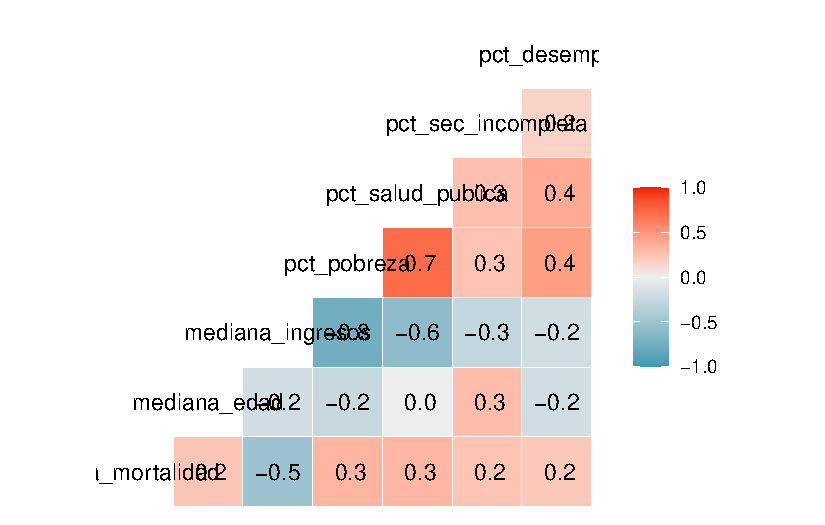
\includegraphics[width=0.85\linewidth,height=\textheight,keepaspectratio]{unidad_3/07_reg_lineal_multiple_files/figure-pdf/ej5-1.pdf}
\end{center}

Como habíamos observado en el capítulo sobre
\hyperref[covarianza-y-correlaciuxf3n]{\textbf{covarianza y
correlación}}, la \texttt{tasa\_mortalidad} tiene correlación negativa
moderada con \texttt{mediana\_ingresos}, también que existe una
correlación negativa fuerte entre \texttt{pct\_pobreza} y
\texttt{mediana\_ingresos} y moderada con \texttt{pct\_salud\_publica}.

\subsection{Estrategia de construcción del
modelo}\label{estrategia-de-construcciuxf3n-del-modelo}

Al momento de seleccionar las variables independientes que formarán
parte del modelo, una de las herramientas más utilizadas es el Criterio
de Información de Akaike (AIC) que ajusta mediante \emph{máxima
verosimilitud}. Al penalizar la complejidad excesiva, el AIC ayuda a
prevenir el sobreajuste y favorece la inclusión de variables relevantes
buscando el modelo equilibrado que describa adecuadamente la relación y
tenga el mínimo AIC. Podemos consultar el AIC de un modelo en R mediante
la función \texttt{AIC()}.

Como vimos anteriormente, la selección de variables se puede hacer
mediante métodos \emph{forward}, \emph{backward} o \emph{stepwise}. La
función \texttt{step()} de R \texttt{base} permite encontrar de forma
automática el mejor modelo basado en AIC utilizando cualquiera de las 3
variantes del método paso a paso. Por otro lado, la función
\texttt{drop1()} de \texttt{R\ base} nos permite realizar un proceso
\emph{backward} manual, eligiendo que variable quitar del modelo en cada
caso según su contribución al AIC. Siempre es oportuno aclarar que estos
últimos métodos se basan en cálculos matemático/estadísticos que no
tienen en cuenta criterios conceptuales epidemiológicos que surjan del
marco teórico, por lo que exigen un control especial del analista.

el lenguaje R ofrece una variedad de funciones para abordar y facilitar
la tarea de seleccionar el mejor modelo de regresión (más parsimonioso).
Como existe correlación fuerte entre \texttt{mediana\_ingresos},
\texttt{pct\_pobreza} y \texttt{pct\_salud\_publica} sólo usaremos la
que presente mayor correlación con \texttt{tasa\_mortalidad}.

\begin{Shaded}
\begin{Highlighting}[]
\CommentTok{\# Modelo saturado}
\NormalTok{mod\_full }\OtherTok{\textless{}{-}} \FunctionTok{lm}\NormalTok{(}
\NormalTok{  tasa\_mortalidad }\SpecialCharTok{\textasciitilde{}}\NormalTok{ mediana\_ingresos }\SpecialCharTok{+}
\NormalTok{    mediana\_edad }\SpecialCharTok{+}
\NormalTok{    pct\_sec\_incompleta }\SpecialCharTok{+}
\NormalTok{    pct\_desempleo }\SpecialCharTok{+}
\NormalTok{    estado,}
  \AttributeTok{data =}\NormalTok{ datos}
\NormalTok{)}

\CommentTok{\# Mediana ingresos}
\NormalTok{mod1 }\OtherTok{\textless{}{-}} \FunctionTok{lm}\NormalTok{(tasa\_mortalidad }\SpecialCharTok{\textasciitilde{}}\NormalTok{ mediana\_ingresos, }\AttributeTok{data =}\NormalTok{ datos)}

\CommentTok{\# Mediana edad}
\NormalTok{mod2 }\OtherTok{\textless{}{-}} \FunctionTok{lm}\NormalTok{(tasa\_mortalidad }\SpecialCharTok{\textasciitilde{}}\NormalTok{ mediana\_edad, }\AttributeTok{data =}\NormalTok{ datos)}

\CommentTok{\# Secundaria incompleta}
\NormalTok{mod3 }\OtherTok{\textless{}{-}} \FunctionTok{lm}\NormalTok{(tasa\_mortalidad }\SpecialCharTok{\textasciitilde{}}\NormalTok{ pct\_sec\_incompleta, }\AttributeTok{data =}\NormalTok{ datos)}

\CommentTok{\# Desempleo}
\NormalTok{mod4 }\OtherTok{\textless{}{-}} \FunctionTok{lm}\NormalTok{(tasa\_mortalidad }\SpecialCharTok{\textasciitilde{}}\NormalTok{ pct\_desempleo, }\AttributeTok{data =}\NormalTok{ datos)}

\CommentTok{\# Estado}
\NormalTok{mod5 }\OtherTok{\textless{}{-}} \FunctionTok{lm}\NormalTok{(tasa\_mortalidad }\SpecialCharTok{\textasciitilde{}}\NormalTok{ estado, }\AttributeTok{data =}\NormalTok{ datos)}
\end{Highlighting}
\end{Shaded}

Mediante \texttt{summary()} observamos sus resultados:

\begin{Shaded}
\begin{Highlighting}[]
\CommentTok{\# Modelo saturado}
\FunctionTok{summary}\NormalTok{(mod\_full)}
\end{Highlighting}
\end{Shaded}

\begin{verbatim}

Call:
lm(formula = tasa_mortalidad ~ mediana_ingresos + mediana_edad + 
    pct_sec_incompleta + pct_desempleo + estado, data = datos)

Residuals:
    Min      1Q  Median      3Q     Max 
-31.475  -7.254   1.161   7.192  29.261 

Coefficients:
                      Estimate Std. Error t value Pr(>|t|)    
(Intercept)          1.488e+02  1.487e+01  10.006  < 2e-16 ***
mediana_ingresos    -3.810e-04  8.165e-05  -4.666 5.62e-06 ***
mediana_edad         5.005e-01  2.588e-01   1.934  0.05453 .  
pct_sec_incompleta   1.652e-01  1.945e-01   0.849  0.39681    
pct_desempleo        1.643e+00  5.781e-01   2.842  0.00494 ** 
estadoMaine          1.462e+01  5.662e+00   2.582  0.01054 *  
estadoMassachusetts  6.389e+00  5.344e+00   1.196  0.23328    
estadoNew Hampshire  1.166e+01  5.963e+00   1.955  0.05198 .  
estadoNew Jersey     1.020e+01  5.010e+00   2.036  0.04302 *  
estadoNew York       7.909e+00  4.706e+00   1.680  0.09443 .  
estadoPennsylvania   9.905e+00  4.867e+00   2.035  0.04315 *  
estadoRhode Island   5.131e+00  7.359e+00   0.697  0.48646    
estadoVermont        1.325e+01  5.814e+00   2.278  0.02377 *  
---
Signif. codes:  0 '***' 0.001 '**' 0.01 '*' 0.05 '.' 0.1 ' ' 1

Residual standard error: 11.93 on 200 degrees of freedom
Multiple R-squared:  0.3373,    Adjusted R-squared:  0.2975 
F-statistic: 8.483 on 12 and 200 DF,  p-value: 6.303e-13
\end{verbatim}

\begin{Shaded}
\begin{Highlighting}[]
\CommentTok{\# Modelos simples}
\FunctionTok{summary}\NormalTok{(mod1)}
\end{Highlighting}
\end{Shaded}

\begin{verbatim}

Call:
lm(formula = tasa_mortalidad ~ mediana_ingresos, data = datos)

Residuals:
    Min      1Q  Median      3Q     Max 
-33.040  -8.210   1.093   7.637  35.932 

Coefficients:
                   Estimate Std. Error t value Pr(>|t|)    
(Intercept)       2.014e+02  3.521e+00  57.200  < 2e-16 ***
mediana_ingresos -5.200e-04  6.133e-05  -8.479 3.94e-15 ***
---
Signif. codes:  0 '***' 0.001 '**' 0.01 '*' 0.05 '.' 0.1 ' ' 1

Residual standard error: 12.32 on 211 degrees of freedom
Multiple R-squared:  0.2542,    Adjusted R-squared:  0.2506 
F-statistic:  71.9 on 1 and 211 DF,  p-value: 3.938e-15
\end{verbatim}

\begin{Shaded}
\begin{Highlighting}[]
\FunctionTok{summary}\NormalTok{(mod2)}
\end{Highlighting}
\end{Shaded}

\begin{verbatim}

Call:
lm(formula = tasa_mortalidad ~ mediana_edad, data = datos)

Residuals:
    Min      1Q  Median      3Q     Max 
-31.870  -9.631   0.512   9.539  46.770 

Coefficients:
             Estimate Std. Error t value Pr(>|t|)    
(Intercept)  134.7306    10.9761  12.275  < 2e-16 ***
mediana_edad   0.8961     0.2600   3.447 0.000684 ***
---
Signif. codes:  0 '***' 0.001 '**' 0.01 '*' 0.05 '.' 0.1 ' ' 1

Residual standard error: 13.88 on 211 degrees of freedom
Multiple R-squared:  0.05332,   Adjusted R-squared:  0.04883 
F-statistic: 11.88 on 1 and 211 DF,  p-value: 0.0006835
\end{verbatim}

\begin{Shaded}
\begin{Highlighting}[]
\FunctionTok{summary}\NormalTok{(mod3)}
\end{Highlighting}
\end{Shaded}

\begin{verbatim}

Call:
lm(formula = tasa_mortalidad ~ pct_sec_incompleta, data = datos)

Residuals:
    Min      1Q  Median      3Q     Max 
-33.903  -9.319   1.485   9.185  41.404 

Coefficients:
                   Estimate Std. Error t value Pr(>|t|)    
(Intercept)        162.9089     2.8037  58.106  < 2e-16 ***
pct_sec_incompleta   0.7202     0.1997   3.607 0.000387 ***
---
Signif. codes:  0 '***' 0.001 '**' 0.01 '*' 0.05 '.' 0.1 ' ' 1

Residual standard error: 13.84 on 211 degrees of freedom
Multiple R-squared:  0.05808,   Adjusted R-squared:  0.05362 
F-statistic: 13.01 on 1 and 211 DF,  p-value: 0.0003867
\end{verbatim}

\begin{Shaded}
\begin{Highlighting}[]
\FunctionTok{summary}\NormalTok{(mod4)}
\end{Highlighting}
\end{Shaded}

\begin{verbatim}

Call:
lm(formula = tasa_mortalidad ~ pct_desempleo, data = datos)

Residuals:
    Min      1Q  Median      3Q     Max 
-35.594  -8.948   0.508   9.029  40.157 

Coefficients:
              Estimate Std. Error t value Pr(>|t|)    
(Intercept)   158.9950     4.1741  38.091  < 2e-16 ***
pct_desempleo   1.7906     0.5418   3.305  0.00112 ** 
---
Signif. codes:  0 '***' 0.001 '**' 0.01 '*' 0.05 '.' 0.1 ' ' 1

Residual standard error: 13.91 on 211 degrees of freedom
Multiple R-squared:  0.04922,   Adjusted R-squared:  0.04471 
F-statistic: 10.92 on 1 and 211 DF,  p-value: 0.001117
\end{verbatim}

\begin{Shaded}
\begin{Highlighting}[]
\FunctionTok{summary}\NormalTok{(mod5)}
\end{Highlighting}
\end{Shaded}

\begin{verbatim}

Call:
lm(formula = tasa_mortalidad ~ estado, data = datos)

Residuals:
    Min      1Q  Median      3Q     Max 
-32.840  -9.533   0.360   9.100  36.641 

Coefficients:
                    Estimate Std. Error t value Pr(>|t|)    
(Intercept)          157.713      4.785  32.960  < 2e-16 ***
estadoMaine           25.438      5.860   4.341 2.24e-05 ***
estadoMassachusetts    7.087      5.998   1.182 0.238741    
estadoNew Hampshire   13.167      6.420   2.051 0.041533 *  
estadoNew Jersey      10.921      5.623   1.942 0.053491 .  
estadoNew York        13.928      5.084   2.739 0.006700 ** 
estadoPennsylvania    17.347      5.075   3.418 0.000762 ***
estadoRhode Island     8.263      8.288   0.997 0.319968    
estadoVermont         18.559      5.998   3.094 0.002251 ** 
---
Signif. codes:  0 '***' 0.001 '**' 0.01 '*' 0.05 '.' 0.1 ' ' 1

Residual standard error: 13.53 on 204 degrees of freedom
Multiple R-squared:  0.1297,    Adjusted R-squared:  0.09555 
F-statistic:   3.8 on 8 and 204 DF,  p-value: 0.0003514
\end{verbatim}

En los resúmenes observamos que todos los coeficientes de las variables
involucradas son significativas y que los valores mostrados tienen forma
de lista, es decir no son tablas ``ordenadas'', por lo que muchas veces
cuando trabajamos con numerosas variables, se hace difícil la
comparación de resultados.

\subsection{Comparación de modelos}\label{comparaciuxf3n-de-modelos}

El comando \texttt{compare\_performance()} del paquete
\texttt{performance} permite comparar de manera sencilla entre modelos
anidados:

\begin{Shaded}
\begin{Highlighting}[]
\FunctionTok{compare\_performance}\NormalTok{(mod\_full, mod1, mod2, mod3, mod4, mod5, }\AttributeTok{metrics =} \StringTok{"common"}\NormalTok{)}
\end{Highlighting}
\end{Shaded}

\begin{verbatim}
# Comparison of Model Performance Indices

Name     | Model |  AIC (weights) |  BIC (weights) |    R2 | R2 (adj.) |   RMSE
-------------------------------------------------------------------------------
mod_full |    lm | 1675.0 (0.830) | 1722.1 (<.001) | 0.337 |     0.298 | 11.557
mod1     |    lm | 1678.2 (0.170) | 1688.3 (>.999) | 0.254 |     0.251 | 12.261
mod2     |    lm | 1729.0 (<.001) | 1739.1 (<.001) | 0.053 |     0.049 | 13.814
mod3     |    lm | 1727.9 (<.001) | 1738.0 (<.001) | 0.058 |     0.054 | 13.779
mod4     |    lm | 1729.9 (<.001) | 1740.0 (<.001) | 0.049 |     0.045 | 13.844
mod5     |    lm | 1725.1 (<.001) | 1758.7 (<.001) | 0.130 |     0.096 | 13.245
\end{verbatim}

Las métricas comunes extraídas de los objetos de regresión, presentadas
en una tabla, son:

\begin{itemize}
\item
  \texttt{AIC}: Criterio de información de Akaike
\item
  \texttt{BIC}: Criterio de información bayesiano
\item
  \texttt{R2}: Coeficiente de determinación \(R^2\)
\item
  \texttt{R2\ (adj.)}: Coeficiente de determinación ajustado
\item
  \texttt{RMSE:} Error cuadrático medio
\end{itemize}

También podemos ordenar los modelos de mejor a peor con el argumento
\texttt{rank\ =\ TRUE}:

\begin{Shaded}
\begin{Highlighting}[]
\FunctionTok{compare\_performance}\NormalTok{(}
\NormalTok{  mod\_full,}
\NormalTok{  mod1,}
\NormalTok{  mod2,}
\NormalTok{  mod3,}
\NormalTok{  mod4,}
\NormalTok{  mod5,}
  \AttributeTok{metrics =} \StringTok{"common"}\NormalTok{,}
  \AttributeTok{rank =} \ConstantTok{TRUE}
\NormalTok{)}
\end{Highlighting}
\end{Shaded}

\begin{verbatim}
# Comparison of Model Performance Indices

Name     | Model |    R2 | R2 (adj.) |   RMSE | AIC weights | BIC weights | Performance-Score
---------------------------------------------------------------------------------------------
mod_full |    lm | 0.337 |     0.298 | 11.557 |       0.830 |    4.58e-08 |            80.00%
mod1     |    lm | 0.254 |     0.251 | 12.261 |       0.170 |       1.000 |            68.44%
mod5     |    lm | 0.130 |     0.096 | 13.245 |    1.12e-11 |    5.15e-16 |            14.85%
mod3     |    lm | 0.058 |     0.054 | 13.779 |    2.71e-12 |    1.60e-11 |             1.89%
mod2     |    lm | 0.053 |     0.049 | 13.814 |    1.59e-12 |    9.36e-12 |             0.87%
mod4     |    lm | 0.049 |     0.045 | 13.844 |    1.00e-12 |    5.90e-12 |         1.18e-10%
\end{verbatim}

Podemos ver que el modelo saturado tiene un menor AIC y
\emph{performance} global que los modelos univariados.

\subsection{Colinealidad}\label{colinealidad-1}

Hay varias maneras de detectar la presencia de colinealidad entre
variables independientes:

\begin{itemize}
\item
  Antes de ajustar el modelo, al comparar los coeficientes de
  correlación.
\item
  Una vez ajustado el modelo, si tenemos un \(R^2\) alto y muchas
  variables independientes que no son estadísticamente significativas.
\end{itemize}

Cuando hemos intuido que tenemos multicolinealidad y queremos comprobar,
el paquete \texttt{performance} nos ofrece la función
\texttt{check\_collinearity()} que implementa el método de factor de
inflación de la varianza (VIF):

\begin{Shaded}
\begin{Highlighting}[]
\FunctionTok{check\_collinearity}\NormalTok{(mod\_full)}
\end{Highlighting}
\end{Shaded}

\begin{verbatim}
# Check for Multicollinearity

Low Correlation

               Term  VIF   VIF 95% CI adj. VIF Tolerance Tolerance 95% CI
   mediana_ingresos 1.89 [1.60, 2.31]     1.38      0.53     [0.43, 0.62]
       mediana_edad 1.34 [1.19, 1.63]     1.16      0.75     [0.61, 0.84]
 pct_sec_incompleta 1.28 [1.14, 1.56]     1.13      0.78     [0.64, 0.88]
      pct_desempleo 1.55 [1.34, 1.88]     1.24      0.65     [0.53, 0.75]
             estado 2.52 [2.09, 3.12]     1.59      0.40     [0.32, 0.48]
\end{verbatim}

Los resultados del ejemplo muestra VIF de entre 1.28 y 2.52 (no hay
colinealidad). Recordemos que el umbral de detección parte de valores
cercanos a 5 y un \(VIF \geq 10\) indicaría que el modelo de regresión
lineal presenta un grado de multicolinealidad preocupante.

\subsection{Análisis de residuales}\label{anuxe1lisis-de-residuales-1}

Como vimos para la regresión lineal simple, podemos analizar
gráficamente los residuales con la función \texttt{check\_model()} del
paquete \texttt{performance}:

\begin{Shaded}
\begin{Highlighting}[]
\FunctionTok{check\_model}\NormalTok{(mod\_full)}
\end{Highlighting}
\end{Shaded}

Por otra parte, también tenemos las funciones de análisis para los
supuestos (independencia, linealidad, normalidad, homocedasticidad).

\begin{itemize}
\tightlist
\item
  \textbf{Independencia:} El paquete \texttt{lmtest} permite evaluar
  independencia según estadístico de Durbin-Watson.
\end{itemize}

\begin{Shaded}
\begin{Highlighting}[]
\FunctionTok{dwtest}\NormalTok{(mod\_full)}
\end{Highlighting}
\end{Shaded}

\begin{verbatim}

    Durbin-Watson test

data:  mod_full
DW = 2.1769, p-value = 0.7772
alternative hypothesis: true autocorrelation is greater than 0
\end{verbatim}

\begin{itemize}
\tightlist
\item
  \textbf{Linealidad:} El paquete \texttt{lmtest} implementa el
  \emph{Ramsey's RESET} bajo la función \texttt{resettest()}
\end{itemize}

\begin{Shaded}
\begin{Highlighting}[]
\FunctionTok{resettest}\NormalTok{(mod\_full)}
\end{Highlighting}
\end{Shaded}

\begin{verbatim}

    RESET test

data:  mod_full
RESET = 0.66971, df1 = 2, df2 = 198, p-value = 0.513
\end{verbatim}

\begin{itemize}
\tightlist
\item
  \textbf{Normalidad:} El paquete \texttt{nortest} permite chequear
  normalidad mediante test de Lilliefors.
\end{itemize}

\begin{Shaded}
\begin{Highlighting}[]
\FunctionTok{lillie.test}\NormalTok{(mod\_full}\SpecialCharTok{$}\NormalTok{residuals)}
\end{Highlighting}
\end{Shaded}

\begin{verbatim}

    Lilliefors (Kolmogorov-Smirnov) normality test

data:  mod_full$residuals
D = 0.060065, p-value = 0.05954
\end{verbatim}

\begin{itemize}
\tightlist
\item
  \textbf{Homocedasticidad:} El paquete \texttt{performance} permite
  chequear homocedasticidad con el test de Breush-Pagan.
\end{itemize}

\begin{Shaded}
\begin{Highlighting}[]
\FunctionTok{check\_heteroscedasticity}\NormalTok{(mod\_full)}
\end{Highlighting}
\end{Shaded}

\begin{verbatim}
Warning: Heteroscedasticity (non-constant error variance) detected (p = 0.012).
\end{verbatim}

Finalmente presentamos un paquete interesante para validar supuestos de
modelos lineales denominado \texttt{gvlma}(Pena y Slate 2019). Su
función, de mismo nombre \texttt{gvlma()}, implementa un procedimiento
global sobre vector residual estandarizado para probar los cuatro
supuestos del modelo lineal.

Si el procedimiento global indica una violación de al menos uno de los
supuestos, los componentes se pueden utilizar para obtener información
sobre qué supuestos se han violado.

\begin{Shaded}
\begin{Highlighting}[]
\FunctionTok{gvlma}\NormalTok{(mod\_full)}
\end{Highlighting}
\end{Shaded}

\begin{verbatim}

Call:
lm(formula = tasa_mortalidad ~ mediana_ingresos + mediana_edad + 
    pct_sec_incompleta + pct_desempleo + estado, data = datos)

Coefficients:
        (Intercept)     mediana_ingresos         mediana_edad  
         148.784543            -0.000381             0.500486  
 pct_sec_incompleta        pct_desempleo          estadoMaine  
           0.165173             1.643031            14.617808  
estadoMassachusetts  estadoNew Hampshire     estadoNew Jersey  
           6.388818            11.657941            10.203316  
     estadoNew York   estadoPennsylvania   estadoRhode Island  
           7.908722             9.905042             5.131109  
      estadoVermont  
          13.245742  


ASSESSMENT OF THE LINEAR MODEL ASSUMPTIONS
USING THE GLOBAL TEST ON 4 DEGREES-OF-FREEDOM:
Level of Significance =  0.05 

Call:
 gvlma(x = mod_full) 

                    Value p-value                Decision
Global Stat        2.3043  0.6800 Assumptions acceptable.
Skewness           0.9587  0.3275 Assumptions acceptable.
Kurtosis           0.0572  0.8110 Assumptions acceptable.
Link Function      0.4246  0.5147 Assumptions acceptable.
Heteroscedasticity 0.8639  0.3527 Assumptions acceptable.
\end{verbatim}

\subsection{Resumen del mejor modelo
elegido}\label{resumen-del-mejor-modelo-elegido}

\begin{Shaded}
\begin{Highlighting}[]
\FunctionTok{summary}\NormalTok{(mod\_full)}
\end{Highlighting}
\end{Shaded}

\begin{verbatim}

Call:
lm(formula = tasa_mortalidad ~ mediana_ingresos + mediana_edad + 
    pct_sec_incompleta + pct_desempleo + estado, data = datos)

Residuals:
    Min      1Q  Median      3Q     Max 
-31.475  -7.254   1.161   7.192  29.261 

Coefficients:
                      Estimate Std. Error t value Pr(>|t|)    
(Intercept)          1.488e+02  1.487e+01  10.006  < 2e-16 ***
mediana_ingresos    -3.810e-04  8.165e-05  -4.666 5.62e-06 ***
mediana_edad         5.005e-01  2.588e-01   1.934  0.05453 .  
pct_sec_incompleta   1.652e-01  1.945e-01   0.849  0.39681    
pct_desempleo        1.643e+00  5.781e-01   2.842  0.00494 ** 
estadoMaine          1.462e+01  5.662e+00   2.582  0.01054 *  
estadoMassachusetts  6.389e+00  5.344e+00   1.196  0.23328    
estadoNew Hampshire  1.166e+01  5.963e+00   1.955  0.05198 .  
estadoNew Jersey     1.020e+01  5.010e+00   2.036  0.04302 *  
estadoNew York       7.909e+00  4.706e+00   1.680  0.09443 .  
estadoPennsylvania   9.905e+00  4.867e+00   2.035  0.04315 *  
estadoRhode Island   5.131e+00  7.359e+00   0.697  0.48646    
estadoVermont        1.325e+01  5.814e+00   2.278  0.02377 *  
---
Signif. codes:  0 '***' 0.001 '**' 0.01 '*' 0.05 '.' 0.1 ' ' 1

Residual standard error: 11.93 on 200 degrees of freedom
Multiple R-squared:  0.3373,    Adjusted R-squared:  0.2975 
F-statistic: 8.483 on 12 and 200 DF,  p-value: 6.303e-13
\end{verbatim}

El modelo \texttt{mod\_full} es capaz de explicar el 29,8\% de la
variabilidad observada en la tasa de mortalidad por cáncer en estos
condados (\(R^2_{ajustado} = 0,2975\)). El test \(F\) global muestra que
es significativo (\(p< 0,001\)).

Los coeficientes se pueden interpretar como:

\begin{itemize}
\item
  \textbf{Mediana de ingresos}: Cada aumento de una unidad en la mediana
  de ingresos reduce la tasa de mortalidad en 0,0004 unidades.
\item
  \textbf{Mediana de edad}: Cuando aumento una unidad en la mediana de
  edad incrementa la tasa de mortalidad en 0,5 unidades.
\item
  \textbf{Porcentaje de población con secundaria incompleta}: Cada
  aumento de una unidad en este porcentaje incrementa la tasa de
  mortalidad en 0,17 unidades, pero esta relación no es significativa.
\item
  \textbf{Porcentaje de desempleo}: Cada aumento de una unidad en el
  desempleo incrementa la tasa de mortalidad en 1.64 unidades.
\item
  \textbf{Estados}: Las tasas de mortalidad varían entre los estados,
  con algunos efectos significativos, como en Maine, New Jersey,
  Pennsylvania y Vermont, todos con tasas de mortalidad más altas que el
  estado de referencia. Es decir, la recta de regresión para cada estado
  tendrá un intercepto diferente.
\end{itemize}

\section{Funciones para modelado
automático}\label{funciones-para-modelado-automuxe1tico}

El uso de la función \texttt{step()} se enmarca en los procedimientos
automáticos y puede ser \emph{forward}, \emph{backward} o mixto. La
sintaxis básica de la función es:

\begin{Shaded}
\begin{Highlighting}[]
\FunctionTok{step}\NormalTok{(}\AttributeTok{object =}\NormalTok{ modelo, }\AttributeTok{direction =} \FunctionTok{c}\NormalTok{(}\StringTok{"both"}\NormalTok{, }\StringTok{"backward"}\NormalTok{, }\StringTok{"forward"}\NormalTok{))}
\end{Highlighting}
\end{Shaded}

donde:

\begin{itemize}
\tightlist
\item
  \texttt{object}: es el modelo inicial de regresión lineal (nulo o
  saturado).
\item
  \texttt{direction}: es la dirección que indicamos. Puede ser
  \texttt{"forward"}, \texttt{"backward"} o \texttt{"both"}
  (predeterminado, si no se define).
\end{itemize}

Generalmente conviene partir del modelo saturado y utilizar la dirección
por defecto, donde se usan ambas direcciones.

\begin{Shaded}
\begin{Highlighting}[]
\NormalTok{modelo\_step }\OtherTok{\textless{}{-}} \FunctionTok{step}\NormalTok{(mod\_full, }\AttributeTok{direction =} \StringTok{"both"}\NormalTok{)}
\end{Highlighting}
\end{Shaded}

\begin{verbatim}
Start:  AIC=1068.56
tasa_mortalidad ~ mediana_ingresos + mediana_edad + pct_sec_incompleta + 
    pct_desempleo + estado

                     Df Sum of Sq   RSS    AIC
- estado              8   1470.71 29922 1063.3
- pct_sec_incompleta  1    102.58 28554 1067.3
<none>                            28452 1068.6
- mediana_edad        1    532.09 28984 1070.5
- pct_desempleo       1   1149.28 29601 1075.0
- mediana_ingresos    1   3096.96 31549 1088.6

Step:  AIC=1063.3
tasa_mortalidad ~ mediana_ingresos + mediana_edad + pct_sec_incompleta + 
    pct_desempleo

                     Df Sum of Sq   RSS    AIC
- pct_sec_incompleta  1      79.5 30002 1061.9
<none>                            29922 1063.3
- mediana_edad        1    1033.9 30956 1068.5
- pct_desempleo       1    1036.6 30959 1068.5
+ estado              8    1470.7 28452 1068.6
- mediana_ingresos    1    6922.4 36845 1105.6

Step:  AIC=1061.86
tasa_mortalidad ~ mediana_ingresos + mediana_edad + pct_desempleo

                     Df Sum of Sq   RSS    AIC
<none>                            30002 1061.9
+ pct_sec_incompleta  1      79.5 29922 1063.3
+ estado              8    1447.7 28554 1067.3
- pct_desempleo       1    1176.8 31179 1068.1
- mediana_edad        1    1302.7 31305 1068.9
- mediana_ingresos    1    7528.4 37530 1107.5
\end{verbatim}

Observamos que el proceso automático nos indica que debemos eliminar las
variables explicativas \texttt{pct\_sec\_incompleta} y \texttt{estado}.

\begin{Shaded}
\begin{Highlighting}[]
\FunctionTok{summary}\NormalTok{(modelo\_step)}
\end{Highlighting}
\end{Shaded}

\begin{verbatim}

Call:
lm(formula = tasa_mortalidad ~ mediana_ingresos + mediana_edad + 
    pct_desempleo, data = datos)

Residuals:
    Min      1Q  Median      3Q     Max 
-31.570  -7.621   1.269   7.564  32.218 

Coefficients:
                   Estimate Std. Error t value Pr(>|t|)    
(Intercept)       1.574e+02  1.271e+01  12.388  < 2e-16 ***
mediana_ingresos -4.517e-04  6.237e-05  -7.242 8.34e-12 ***
mediana_edad      7.065e-01  2.345e-01   3.013  0.00291 ** 
pct_desempleo     1.397e+00  4.881e-01   2.863  0.00462 ** 
---
Signif. codes:  0 '***' 0.001 '**' 0.01 '*' 0.05 '.' 0.1 ' ' 1

Residual standard error: 11.98 on 209 degrees of freedom
Multiple R-squared:  0.3012,    Adjusted R-squared:  0.2912 
F-statistic: 30.03 on 3 and 209 DF,  p-value: 3.488e-16
\end{verbatim}

Si bien en el ejemplo mostramos como usar el método \emph{stepwise}
automático para la selección de variables, no se recomienda su uso ya
que está basado únicamente en criterios matemáticos y no en la
relevancia en el mundo real.

Además, cuenta con las siguientes limitaciones:

\begin{itemize}
\item
  Sensibilidad a la selección de variables
\item
  Propensión al sobreajuste
\item
  Violación de supuestos estadísticos
\item
  Inclusión de variables irrelevantes
\end{itemize}

Para evitar estos inconvenientes, es recomendable usar métodos
alternativos de selección de variables tales como:

\begin{itemize}
\item
  \textbf{Selección manual de variables}, según su relevancia teórica y
  conocimiento experto del tema.
\item
  \textbf{Selección de variables por AIC o BIC} (Criterio de Información
  Bayesiano).
\item
  \textbf{Regularización} por regresión LASSO (\emph{Least Absolute
  Shrinkage and Selection Operator}), que penaliza los coeficientes de
  las variables menos importantes, favoreciendo modelos más simples y
  generalizables. Para conocer más sobre este método pueden entrar al
  siguiente enlace:

  ➡️
  \href{https://www.lexjansen.com/pnwsug/2008/DavidCassell-StoppingStepwise.pdf}{\textbf{Stopping
  stepwise}}
\item
  \textbf{Árboles de decisión} (\emph{random forest} y \emph{gradient
  boosting),} herramientas de aprendizaje automático que permiten
  manejar automáticamente la selección de variables con menor
  probabilidad de sobreajuste. Para conocer más sobre este método pueden
  entrar al siguiente enlace:

  ➡️
  \href{https://www.ibm.com/es-es/think/topics/decision-trees}{\textbf{Decision
  trees}}
\end{itemize}

Estos dos últimos métodos escapan al alcance del curso. Sin embargo,
invitamos a quienes tengan interés a explorar las múltiples
posibilidades que ofrecen, en particular al momento de analizar datasets
grandes y con múltiples variables explicativas.

De Irala et~al. (2001a)

De Irala et~al. (2001b)

Gordis (2017)

Kim (2019)

Kleinbaum et~al. (1988)

MacMahon (1972)

Schloerke et~al. (2025)

Zeileis y Hothorn (2002)

\section*{Referencias}\label{referencias-17}
\addcontentsline{toc}{section}{Referencias}

\markright{Referencias}

\protect\phantomsection\label{refs}
\begin{CSLReferences}{1}{1}
\bibitem[\citeproctext]{ref-agresti2015}
Agresti, Alan. 2015. \emph{Foundations of {Linear} and {Generalized}
{Linear} {Models}}. Wiley {Series} en {Probability} y {Statistics}. John
Wiley \& Sons, Inc.

\bibitem[\citeproctext]{ref-almeidafilho2011}
Almeida Filho, Naomar de, y Maurício Lima Barreto. 2011.
\emph{Epidemiologia \& Saúde: Fundamentos, Métodos e Aplicações}.
Guanabara Koogan.

\bibitem[\citeproctext]{ref-alvarez_caceres2007}
Álvarez Cáceres, Rafael. 2007. \emph{Estadística aplicada a las ciencias
de la salud}. Ediciones Díaz de Santos.

\bibitem[\citeproctext]{ref-aycaguer2000}
Aycaguer, Luis Carlos Silva. 2000. \emph{Diseño razonado de muestras y
captación de datos para la investigación sanitaria}. Ediciones Díaz de
Santos.

\bibitem[\citeproctext]{ref-magrittr}
Bache, Stefan Milton, y Hadley Wickham. 2026. \emph{magrittr: A
Forward-Pipe Operator for R}.
\url{https://doi.org/10.32614/CRAN.package.magrittr}.

\bibitem[\citeproctext]{ref-ballester-diez2003}
Ballester Díez, Ferrán, y José María Tenías Burillo. 2003.
\emph{Estudios ecológicos}. Valencia : Escola Valenciana d'Estudis per a
la Salut, 2003.

\bibitem[\citeproctext]{ref-bell2012}
Bell, Bethany A., Anthony J. Onwuegbuzie, John M. Ferron, Qun G. Jiao,
Susan T. Hibbard, y Jeffrey D. Kromrey. 2012. {«Use of {Design}
{Effects} and {Sample} {Weights} in {Complex} {Health} {Survey} {Data}:
{A} {Review} of {Published} {Articles} {Using} {Data} {From} 3
{Commonly} {Used} {Adolescent} {Health} {Surveys}»}. \emph{American
Journal of Public Health} 102 (7): 1399-405.
\url{https://doi.org/10.2105/AJPH.2011.300398}.

\bibitem[\citeproctext]{ref-pwr}
Champely, Stephane. 2020. \emph{pwr: Basic Functions for Power
Analysis}. \url{https://doi.org/10.32614/CRAN.package.pwr}.

\bibitem[\citeproctext]{ref-daniel2002}
Daniel, Wayne W. 2002. \emph{Bioestadística: {Base} para el análisis de
las ciencias de la salud}. 4.ª ed. Limusa Wiley.

\bibitem[\citeproctext]{ref-de_irala2001a}
De Irala, Jokin, Miguel Ángel Martínez-González, y Francisco Guillén
Grima. 2001a. {«¿{Qué} es una variable de confusión?»} \emph{Medicina
Clínica} 117 (10): 377-85.
\url{https://doi.org/10.1016/S0025-7753(01)72121-5}.

\bibitem[\citeproctext]{ref-de_irala2001b}
De Irala, Jokin, Miguel Ángel Martínez-González, y Francisco Guillén
Grima. 2001b. {«¿{Qué} es una variable modificadora del efecto?»}
\emph{Medicina Clínica} 117 (8): 297-302.
\url{https://doi.org/10.1016/S0025-7753(01)72092-1}.

\bibitem[\citeproctext]{ref-vonelm2008}
Elm, Erik von, Douglas G. Altman, Matthias Egger, Stuart J. Pocock,
Peter C. Gøtzsche, y Jan P. Vandenbroucke. 2008. {«The Strengthening the
Reporting of Observational Studies in Epidemiology (STROBE) Statement:
Guidelines for Reporting Observational Studies»}. \emph{Journal of
Clinical Epidemiology} 61 (4): 344-49.
\url{https://doi.org/10.1016/j.jclinepi.2007.11.008}.

\bibitem[\citeproctext]{ref-epidat}
\emph{{EPIDAT} 4.2 - {Consellería} de {Sanidade} - {Servizo} {Galego} de
{Saúde}}. s.~f. Accedido 11 de junio de 2024.
\url{https://www.sergas.es/Saude-publica/EPIDAT-4-2}.

\bibitem[\citeproctext]{ref-field2014}
Field, Andy, Jeremy Miles, y Zoë Field. 2014. \emph{Discovering
statistics using {R}}. Repr. Sage.

\bibitem[\citeproctext]{ref-janitor}
Firke, Sam. 2024. \emph{janitor: Simple Tools for Examining and Cleaning
Dirty Data}. \url{https://doi.org/10.32614/CRAN.package.janitor}.

\bibitem[\citeproctext]{ref-srvyr}
Freedman Ellis, Greg, y Ben Schneider. 2026. \emph{srvyr: 'dplyr'-Like
Syntax for Summary Statistics of Survey Data}.
\url{https://doi.org/10.32614/CRAN.package.srvyr}.

\bibitem[\citeproctext]{ref-glantz2006}
Glantz, S. 2006. \emph{Bioestadística}. 6.ª ed. McGraw Hill.

\bibitem[\citeproctext]{ref-gordis2017}
Gordis, Leon. 2017. \emph{Epidemiologia}. Thieme Revinter Publicações
LTDA.

\bibitem[\citeproctext]{ref-nortest}
Gross, Juergen, y Uwe Ligges. 2015. \emph{nortest: Tests for Normality}.
\url{https://doi.org/10.32614/CRAN.package.nortest}.

\bibitem[\citeproctext]{ref-gutierrez2020}
Gutiérrez, Andrés, Xavier Mancero, Alvaro Fuentes, Felipe López, y
Felipe Molina. 2020. \emph{Criterios de calidad en la estimación de
indicadores a partir de encuestas de hogares: una aplicación a la
migración internacional}.

\bibitem[\citeproctext]{ref-hernandez-avila2011}
Hernández-Ávila, Mauricio. 2011. \emph{Epidemiología: diseño y análisis
de estudios}. Editorial Médica Panamericana.

\bibitem[\citeproctext]{ref-holmberg2022}
Holmberg, Mathias J., y Lars W. Andersen. 2022. {«Collider Bias»}.
\emph{JAMA} 327 (13): 1282-83.
\url{https://doi.org/10.1001/jama.2022.1820}.

\bibitem[\citeproctext]{ref-ggfortify}
Horikoshi, Masaaki, y Yuan Tang. 2018. \emph{ggfortify: Data
Visualization Tools for Statistical Analysis Results}.
\url{https://CRAN.R-project.org/package=ggfortify}.

\bibitem[\citeproctext]{ref-ggpubr}
Kassambara, Alboukadel. 2026a. \emph{ggpubr: 'ggplot2' Based Publication
Ready Plots}. \url{https://CRAN.R-project.org/package=ggpubr}.

\bibitem[\citeproctext]{ref-rstatix}
Kassambara, Alboukadel. 2026b. \emph{rstatix: Pipe-Friendly Framework
for Basic Statistical Tests}.
\url{https://doi.org/10.32614/CRAN.package.rstatix}.

\bibitem[\citeproctext]{ref-survminer}
Kassambara, Alboukadel, Marcin Kosinski, y Przemyslaw Biecek. 2026.
\emph{survminer: Drawing Survival Curves using 'ggplot2'}.
\url{https://doi.org/10.32614/CRAN.package.survminer}.

\bibitem[\citeproctext]{ref-kim2019}
Kim, Jong Hae. 2019. {«Multicollinearity and Misleading Statistical
Results»}. \emph{Korean Journal of Anesthesiology} 72 (6): 558-69.
\url{https://doi.org/10.4097/kja.19087}.

\bibitem[\citeproctext]{ref-kleinbaum1988}
Kleinbaum, David G, Lawrence L Kupper, Keith E Muller, y Azhar Nizam.
1988. \emph{Applied regression analysis and other multivariable
methods}. Vol. 601. Duxbury press Belmont, CA.

\bibitem[\citeproctext]{ref-moments}
Komsta, Lukasz, y Frederick Novomestky. 2022. \emph{moments: Moments,
Cumulants, Skewness, Kurtosis and Related Tests}.
\url{https://doi.org/10.32614/CRAN.package.moments}.

\bibitem[\citeproctext]{ref-emmeans}
Lenth, Russell V., y Julia Piaskowski. 2026. \emph{emmeans: Estimated
Marginal Means, aka Least-Squares Means}.
\url{https://doi.org/10.32614/CRAN.package.emmeans}.

\bibitem[\citeproctext]{ref-easystats}
Lüdecke, Daniel, Mattan S. Ben-Shachar, Indrajeet Patil, et~al. 2022.
{«easystats: Framework for Easy Statistical Modeling, Visualization, and
Reporting»}. \emph{CRAN}, advance online publication.
\url{https://doi.org/10.32614/CRAN.package.easystats}.

\bibitem[\citeproctext]{ref-see}
Lüdecke, Daniel, Indrajeet Patil, Mattan S. Ben-Shachar, Brenton M.
Wiernik, Philip Waggoner, y Dominique Makowski. 2021. {«{see}: An {R}
Package for Visualizing Statistical Models»}. \emph{Journal of Open
Source Software} 6 (64): 3393.
\url{https://doi.org/10.21105/joss.03393}.

\bibitem[\citeproctext]{ref-survey}
Lumley, Thomas. 2010. \emph{Complex Surveys: A Guide to Analysis Using
R: A Guide to Analysis Using R}. John Wiley; Sons.

\bibitem[\citeproctext]{ref-luque-fernandez2019}
Luque-Fernandez, Miguel Angel, Michael Schomaker, Daniel
Redondo-Sanchez, Maria Jose Sanchez Perez, Anand Vaidya, y Mireille E.
Schnitzer. 2019. {«Educational Note: Paradoxical collider effect in the
analysis of non-communicable disease epidemiological data: a
reproducible illustration and web application»}. \emph{International
Journal of Epidemiology} 48 (2): 640-53.
\url{https://doi.org/10.1093/ije/dyy275}.

\bibitem[\citeproctext]{ref-macmahon1972}
MacMahon, Brian. 1972. {«Concepts of multiple factors»}. \emph{Multiple
factors in the causation of environmentally induced disease. Academic
Press, New York}.

\bibitem[\citeproctext]{ref-samplingbook}
Manitz, Juliane, Mark Hempelmann, Goeran Kauermann, et~al. 2021.
\emph{samplingbook: Survey Sampling Procedures}.
\url{https://doi.org/10.32614/CRAN.package.samplingbook}.

\bibitem[\citeproctext]{ref-esquisse}
Meyer, Fanny, y Victor Perrier. 2025. \emph{esquisse: Explore and
Visualize Your Data Interactively}.
\url{https://doi.org/10.32614/CRAN.package.esquisse}.

\bibitem[\citeproctext]{ref-tibble}
Müller, Kirill, y Hadley Wickham. 2026. \emph{tibble: Simple Data
Frames}. \url{https://doi.org/10.32614/CRAN.package.tibble}.

\bibitem[\citeproctext]{ref-national_research2015}
National Research Council; Division of Behavioral and Social Sciences
and Education. 2015. \emph{Realizing the {Potential} of the {American}
{Community} {Survey}: {Challenges}, {Tradeoffs}, and {Opportunities}}.
National Academies Press. \url{https://doi.org/10.17226/21653}.

\bibitem[\citeproctext]{ref-norman1996}
Norman, GR, y Streiner, DL. 1996. \emph{Bioestadística}. Mosby/Doyma
Libros.

\bibitem[\citeproctext]{ref-patchwork}
Pedersen, Thomas Lin. 2025. \emph{patchwork: The Composer of Plots}.
\url{https://doi.org/10.32614/CRAN.package.patchwork}.

\bibitem[\citeproctext]{ref-scico}
Pedersen, Thomas Lin, y Fabio Crameri. 2023. \emph{scico: Colour
Palettes Based on the Scientific Colour-Maps}.
\url{https://doi.org/10.32614/CRAN.package.scico}.

\bibitem[\citeproctext]{ref-gvlma}
Pena, Edsel A., y Elizabeth H. Slate. 2019. \emph{gvlma: Global
Validation of Linear Models Assumptions}.
\url{https://doi.org/10.32614/CRAN.package.gvlma}.

\bibitem[\citeproctext]{ref-rius_diaz2012}
Ríus Díaz, Francisca, Francisco Javier Barón Lopez, Elisa Sánchez Font,
y Luis Parras Guijosa. 2012. \emph{Bioestadística: {Métodos} y
{Aplicaciones}}.
\url{http://virtual.uptc.edu.co/ova/estadistica/docs/libros/ftp.bioestadistica.uma.es/libro/}.

\bibitem[\citeproctext]{ref-rodriguez2018}
Rodríguez, Milena, y Fredy Mendivelso. 2018. {«Diseño de investigación
de corte transversal»}. \emph{Revista Médica Sanitas} 21 (3): 141-47.
\url{https://revistas.unisanitas.edu.co/index.php/rms/article/view/368}.

\bibitem[\citeproctext]{ref-rodriguez2003}
Rodríguez, VM, Verónica A Martínez Ordaz, José Roiz Hernández, Francisco
Huazano García, y Armando Nieves Rentería. 2003. {«Muestreo y tamaño de
la muestra»}. \emph{Una guía práctica. Coahuila, México: El Cid Editor}.

\bibitem[\citeproctext]{ref-royo-bordonada2009}
Royo-Bordonada, Miguel Angel, Javier Damian, Beatriz Perez-Gomez, et~al.
2009. \emph{Método epidemiológico}. Instituto de Salud Carlos III
(ISCIII). Escuela Nacional de Sanidad (ENS).
\url{http://hdl.handle.net/20.500.12105/5271}.

\bibitem[\citeproctext]{ref-dlookr}
Ryu, Choonghyun. 2025. \emph{{dlookr}: Tools for Data Diagnosis,
Exploration, Transformation}.
\url{https://CRAN.R-project.org/package=dlookr}.

\bibitem[\citeproctext]{ref-sakshaug2014}
Sakshaug, Joseph W., y Brady T. West. 2014. {«Important {Considerations}
{When} {Analyzing} {Health} {Survey} {Data} {Collected} {Using} a
{Complex} {Sample} {Design}»}. \emph{American Journal of Public Health}
104 (1): 15-16. \url{https://doi.org/10.2105/AJPH.2013.301515}.

\bibitem[\citeproctext]{ref-GGally}
Schloerke, Barret, Di Cook, Joseph Larmarange, et~al. 2025.
\emph{GGally: Extension to 'ggplot2'}.
\url{https://doi.org/10.32614/CRAN.package.GGally}.

\bibitem[\citeproctext]{ref-schulz2010}
Schulz, K. F, D. G Altman, y D. Moher. 2010. {«CONSORT 2010 Statement:
Updated Guidelines for Reporting Parallel Group Randomised Trials»}.
\emph{BMJ} 340 (mar23 1): c332-32.
\url{https://doi.org/10.1136/bmj.c332}.

\bibitem[\citeproctext]{ref-gtsummary}
Sjoberg, Daniel D., Karissa Whiting, Michael Curry, Jessica A. Lavery, y
Joseph Larmarange. 2021. {«Reproducible Summary Tables with the
gtsummary Package»}. \emph{{The R Journal}} 13: 570-80.
\url{https://doi.org/10.32614/RJ-2021-053}.

\bibitem[\citeproctext]{ref-epikit}
Spina, Alexander, Zhian N. Kamvar, y Dirk Schumacher. 2025.
\emph{epikit: Miscellaneous Helper Tools for Epidemiologists}.
\url{https://doi.org/10.32614/CRAN.package.epikit}.

\bibitem[\citeproctext]{ref-epiR}
Stevenson, Mark, y Evan Sergeant. 2026. \emph{epiR: Tools for the
Analysis of Epidemiological Data}.
\url{https://doi.org/10.32614/CRAN.package.epiR}.

\bibitem[\citeproctext]{ref-cols4all}
Tennekes, Martijn, y Marco J. H. Puts. 2023. {«{cols4all}: a color
palette analysis tool»}. \emph{EuroVis (Short Papers)}.
\url{https://doi.org/10.2312/evs.20231040}.

\bibitem[\citeproctext]{ref-triola2018}
Triola, Mario F. 2018. \emph{{ESTADÍSTICA} {Decimosegunda} {Edicion}}.
Pearson Educación de México, SA de CV.

\bibitem[\citeproctext]{ref-vancauwenberghe2014}
Van Cauwenberghe, Lisbeth, y Colin R. Janssen. 2014. {«Microplastics in
Bivalves Cultured for Human Consumption»}. \emph{Environmental
Pollution} 193 (octubre): 65-70.
\url{https://doi.org/10.1016/j.envpol.2014.06.010}.

\bibitem[\citeproctext]{ref-skimr}
Waring, Elin, Michael Quinn, Amelia McNamara, Eduardo Arino de la Rubia,
Hao Zhu, y Shannon Ellis. 2026. \emph{skimr: Compact and Flexible
Summaries of Data}. \url{https://doi.org/10.32614/CRAN.package.skimr}.

\bibitem[\citeproctext]{ref-weisberg2005}
Weisberg, Sanford. 2005. \emph{Applied linear regression}. Vol. 528.
John Wiley \& Sons.

\bibitem[\citeproctext]{ref-plyr}
Wickham, Hadley. 2011. {«The Split-Apply-Combine Strategy for Data
Analysis»}. \emph{Journal of Statistical Software} 40 (1): 1-29.
\url{https://www.jstatsoft.org/v40/i01/}.

\bibitem[\citeproctext]{ref-ggplot2}
Wickham, Hadley. 2016. \emph{ggplot2: Elegant Graphics for Data
Analysis}. Springer-Verlag New York.
\url{https://ggplot2.tidyverse.org}.

\bibitem[\citeproctext]{ref-tidyverse}
Wickham, Hadley, Mara Averick, Jennifer Bryan, et~al. 2019. {«Welcome to
the {tidyverse}»}. \emph{Journal of Open Source Software} 4 (43): 1686.
\url{https://doi.org/10.21105/joss.01686}.

\bibitem[\citeproctext]{ref-readxl}
Wickham, Hadley, y Jennifer Bryan. 2026. \emph{readxl: Read Excel
Files}. \url{https://doi.org/10.32614/CRAN.package.readxl}.

\bibitem[\citeproctext]{ref-dplyr}
Wickham, Hadley, Romain François, Lionel Henry, Kirill Müller, y Davis
Vaughan. 2026. \emph{dplyr: A Grammar of Data Manipulation}.
\url{https://doi.org/10.32614/CRAN.package.dplyr}.

\bibitem[\citeproctext]{ref-readr}
Wickham, Hadley, Jim Hester, y Jennifer Bryan. 2026. \emph{readr: Read
Rectangular Text Data}.
\url{https://doi.org/10.32614/CRAN.package.readr}.

\bibitem[\citeproctext]{ref-lmtest}
Zeileis, Achim, y Torsten Hothorn. 2002. {«Diagnostic Checking in
Regression Relationships»}. \emph{R News} 2 (3): 7-10.
\url{https://CRAN.R-project.org/doc/Rnews/}.

\end{CSLReferences}


\backmatter


\end{document}
